\documentclass[preprint,11pt,numbers]{elsarticle-arxiv}
\usepackage{lmodern}
\usepackage{amssymb,amsmath,amsthm,mathtools}
\usepackage{booktabs,enumitem,indentfirst,etoolbox,float,url}
\makeatletter
\IfFileExists{placeins.sty}{\usepackage{placeins}}{%
  \newcommand{\FloatBarrier}{\par\ifx\@deferlist\@empty\else\clearpage\fi}}
\makeatother
\usepackage{tikz}
\usetikzlibrary{arrows.meta}
\tikzset{
  graph vertex/.style={circle,fill=black,inner sep=1.7pt},
  marked edge/.style={draw=blue!65!black,line width=1.05pt},
  unmarked edge/.style={draw=black!65,line width=0.65pt}
}
\usepackage[hidelinks]{hyperref}
\ifdefined\pdfgentounicode
  \InputIfFileExists{glyphtounicode.tex}{}{}
  \pdfgentounicode=1
\fi
\pdfstringdefDisableCommands{\def\corref#1{}\def\fnref#1{}}
\setcitestyle{square,comma}
\numberwithin{equation}{section}
\newtheorem{theorem}{Theorem}[section]
\newtheorem{conjecture}[theorem]{Conjecture}
\newtheorem{lemma}[theorem]{Lemma}
\theoremstyle{definition}
\newtheorem{defn}[theorem]{Definition}
\DeclareMathOperator{\tr}{tr}
\newenvironment{lateproof}[1]{\begin{proof}[Proof of #1]}{\end{proof}}
\newcommand{\papertitle}{The Proof of the Faudree--Gy\'arf\'as--Schelp--Tuza Conjecture}
\hypersetup{pdftitle={\papertitle},pdfauthor={Zhijun Lu, Chengshuo Qiao, Qirui Ying, Huimin Song}}
\setlist[enumerate]{itemsep=3pt,topsep=5pt,parsep=0pt,listparindent=1.5em}
\setlength{\emergencystretch}{2em}
\setlength{\parindent}{1.5em}
\setcounter{tocdepth}{2}
\patchcmd{\abstract}
  {\par\medskip\noindent\unskip\ignorespaces}
  {\par\medskip\ignorespaces}
  {}{\PackageError{manuscript}{Could not apply abstract indentation}{}}

% Appendix references point to fgst_conjecture.pdf when both PDFs are kept together.
\newlabel{app:cycle-estimates}{{C}{}{}{subsection.appendix.3}{fgst_conjecture.pdf}}
\newlabel{app:data-specification}{{A}{}{}{subsection.appendix.1}{fgst_conjecture.pdf}}
\newlabel{app:flag-lists}{{A.2}{}{}{subsubsection.appendix.1.2}{fgst_conjecture.pdf}}
\newlabel{app:multi-low-degree}{{F.1}{}{}{subsubsection.appendix.6.1}{fgst_conjecture.pdf}}
\newlabel{app:multi-nine}{{F.2}{}{}{subsubsection.appendix.6.2}{fgst_conjecture.pdf}}
\newlabel{app:multi-projection}{{G.1}{}{}{subsubsection.appendix.7.1}{fgst_conjecture.pdf}}
\newlabel{app:multi-structure}{{E}{}{}{subsection.appendix.5}{fgst_conjecture.pdf}}
\newlabel{app:odd-small}{{D}{}{}{subsection.appendix.4}{fgst_conjecture.pdf}}
\newlabel{app:ore-replay}{{B.3}{}{}{subsubsection.appendix.2.3}{fgst_conjecture.pdf}}
\newlabel{app:pattern-indices}{{A.1}{}{}{subsubsection.appendix.1.1}{fgst_conjecture.pdf}}
\newlabel{app:profile-verification}{{G.3}{}{}{subsubsection.appendix.7.3}{fgst_conjecture.pdf}}
\newlabel{app:reproduction}{{B}{}{}{subsection.appendix.2}{fgst_conjecture.pdf}}
\newlabel{app:weighted-final-checks}{{G.4}{}{}{subsubsection.appendix.7.4}{fgst_conjecture.pdf}}
\newlabel{tab:blocks}{{A.2}{}{}{table.supp.A.2}{fgst_conjecture.pdf}}
\newlabel{tab:thirteen-cover-check}{{E.1}{}{}{table.supp.E.1}{fgst_conjecture.pdf}}
\begin{document}
\bibliographystyle{alpha}
\begin{frontmatter}
\title{\textbf{\Large\papertitle}}
\author[1]{Zhijun Lu\fnref{equalcontrib}}
\author[1]{Chengshuo Qiao\fnref{equalcontrib}}
\author[1]{Qirui Ying\fnref{equalcontrib}}
\author[1]{Huimin Song\corref{cor1}}
\fntext[equalcontrib]{Zhijun Lu, Chengshuo Qiao and Qirui Ying contributed equally to this work.}
\cortext[cor1]{Corresponding author. \textit{E-mail address:}
\url{hmsong@sdu.edu.cn} (H.Song).}
\affiliation[1]{organization={School of Mathematics and Statistics},
 addressline={Shandong University},city={Weihai},postcode={264209},
 state={Shandong},country={China}}

\begin{abstract}
In 1990, Faudree, Gy\'arf\'as, Schelp and Tuza proposed a relaxation
of the strong edge-coloring conjecture. They conjectured that every
finite loopless multigraph $G$ satisfies
$\omega(L(G)^2)\leq\Delta^2+\lfloor\frac{\Delta}{2}\rfloor^2$, where
$\Delta=\Delta(G)$ is the maximum degree, $L(G)$ is the line graph
of $G$, and $\omega$ is the clique number. In this paper, we prove this conjecture. We first use the flag algebra
method to show that $\omega(L(G)^2)\leq\frac{5}{4}\Delta^2$ for every
finite loopless multigraph $G$. This settles the even-degree case.
For odd $\Delta\geq 9$, we show that if
$\omega(L(G)^2)>\Delta^2+\lfloor\frac{\Delta}{2}\rfloor^2$,
then $L(G)^2$ has a clique exceeding this bound whose vertices
correspond to a set of edges of $G$ that includes both a pair of
parallel edges and five edges forming an induced five-cycle in the
underlying simple graph of $G$. Counting around such cycles gives a
bound that contradicts the weighted flag inequalities. The remaining
small degrees are handled separately, thereby completing the proof.
\end{abstract}
\begin{keyword}
\textit{Squares of line graphs \sep clique number \sep flag algebras}
\end{keyword}
\end{frontmatter}

\thispagestyle{plain}
\tableofcontents
\clearpage
\section{Introduction}\label{sec:intro}

\subsection{Preliminaries}\label{sec:prelim}

All graphs are finite and simple unless stated otherwise. In a loopless
multigraph, parallel edges are distinct and contribute to degrees with
multiplicity. For a graph $G$, write $V(G)$, $E(G)$ and $\Delta(G)$ for
its vertex set, edge set and maximum degree. For $v\in V(G)$, let
$N_G(v)$ be its set of neighbors and let $d_G(v)$ be its degree.
For $X\subseteq V(G)$, write $G[X]$ for the subgraph induced by $X$ and
$d_G(v,X)$ for the number of edges from $v$ to $X$. Let $N_G[v]=N_G(v)\cup\{v\}$.
%We take $\Delta(G)=0$ for a graph with no vertices. We use $\Delta$ for the maximum degree of a fixed graph and $D$ when retaining the original degree bound after restricting the graph. 
A graph is
$d$-regular if all its vertices have degree $d$. An ordered edge is an
edge together with an ordering of its endpoints.
Write $C_n$ for the cycle on $n\geq 3$ vertices, $K_n$ for the complete
graph on $n$ vertices, and $K_{a,b}$ for the complete bipartite graph with
parts of sizes $a$ and $b$.

A vertex cover of $G$ is a set meeting every edge, and $\tau(G)$ is
the minimum size of a vertex cover. An independent set is a set of
pairwise nonadjacent vertices. For a subgraph $H$ of $G$ with at least
one edge, its Ore-degree in $G$ is
$\max_{uv\in E(H)}(d_G(u)+d_G(v))$~\cite{FaronPostle2019}.
We put $x_+=\max\{x,0\}$ for real $x$.

The \emph{underlying simple graph} of a loopless multigraph $G$, also
called its \emph{simple support}, has vertex set $V(G)$ and one edge
$uv$ for each pair of distinct vertices $u,v$ joined by an edge of $G$.
The line graph $L(G)$ has
one vertex for each edge of $G$, with two distinct edges adjacent
precisely when they share an endpoint in $G$. For a graph $H$,
its square $H^2$ has vertex set $V(H)$, with two distinct vertices
adjacent precisely when $H$ contains a path of length at most two
between them. We write $\omega(H)$ for the maximum size of a clique in
$H$, that is, a set of pairwise adjacent vertices. A set
$S\subseteq E(G)$ is a \emph{strong clique} in $G$ if it is a clique
in $L(G)^2$.
%Equivalently, any two distinct edges of $S$ share an endpoint or have endpoints joined by an edge of $G$.

For a positive integer $k$, write $[k]=\{1,\ldots,k\}$. A proper vertex
$k$-coloring of $H$ is a map $V(H)\to[k]$ assigning distinct colors to
adjacent vertices. The chromatic number $\chi(H)$ is the least $k$ for
which $H$ admits such a coloring, with $\chi(H)=0$ when $V(H)$ is empty.
A proper vertex coloring of $L(G)^2$ gives a \emph{strong edge
coloring} of $G$. The minimum number of colors in such a coloring is
the \emph{strong chromatic index} $\chi(L(G)^2)$.

A real symmetric matrix $M$ is positive semidefinite, written
$M\succeq0$, if $x^{\mathsf T}Mx\geq0$ for every real column vector
$x$ of the appropriate size. The trace $\tr(M)$ of a square matrix
$M$ is the sum of its diagonal entries.

\subsection{Background and Main Result}\label{sec:background}

In 1985, at a seminar in Prague, Erd\H{o}s and Ne\v{s}et\v{r}il asked
how large the strong chromatic index can be for a graph of given
maximum degree~\cite{FGST1989,ErdosNesetril1989}. Erd\H{o}s~\cite{Erdos1988}
stated their conjecture with the bound $\frac{5}{4}\Delta(G)^2$.
Faudree, Schelp, Gy\'arf\'as and Tuza~\cite{FGST1990} formulated a
version for loopless multigraphs that gives a sharper bound for odd
maximum degree. For a nonnegative integer $d$, let
$f(d)=d^2+\lfloor\frac{d}{2}\rfloor^2$. Thus $f(d)=\frac{5d^2}{4}$
when $d$ is even and $f(d)=\frac{5d^2-2d+1}{4}$ when $d$ is odd.

\begin{conjecture}[\cite{FGST1990}]
\label{conj:strong-edge-coloring}
Every finite loopless multigraph $G$ satisfies
$\chi(L(G)^2)\leq f(\Delta(G))$.
\end{conjecture}

Faudree, Gy\'arf\'as, Schelp and Tuza also asked how large a set of edges
forced to have distinct colors can be. Hence, they proposed the following
relaxation of \textbf{Conjecture~\ref{conj:strong-edge-coloring}}.

\begin{conjecture}[\cite{FGST1990}]\label{conj:fgst}
Every finite loopless multigraph $G$ satisfies
$\omega(L(G)^2)\leq f(\Delta(G))$.
\end{conjecture}

In this paper, we prove \textbf{Conjecture~\ref{conj:fgst}}.

\begin{theorem}\label{thm:multigraph}
Every finite loopless multigraph $G$ satisfies
$\omega(L(G)^2)\leq f(\Delta(G))$.
\end{theorem}

Blow-ups of a five-cycle attain the bound. Let $C_5=v_0v_1v_2v_3v_4v_0$. Replace each $v_i$ by an independent set $V_i$ and add every edge between $V_i$ and $V_{i+1}$, with indices taken modulo five. It is easy to see that the entire edge set of the blow-up is a strong clique. Taking $|V_i|=t$ for each $i$ gives
maximum degree $2t$ and $5t^2=f(2t)$ edges, as illustrated for
$t=2$ in Figure~\ref{fig:blowup}. Taking $|V_2|=|V_3|=r+1$ and
$|V_0|=|V_1|=|V_4|=r$ gives maximum degree $2r+1$ and
$5r^2+4r+1=f(2r+1)$ edges, as required.

\begin{figure}[!htbp]
\centering
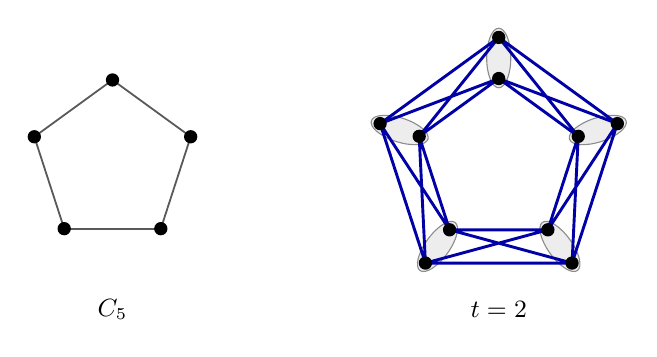
\begin{tikzpicture}[scale=0.9,every node/.style={font=\small}]
\foreach \i in {0,...,4}
  \coordinate (v\i) at ({90+72*\i}:1.16);
\foreach \i/\j in {0/1,1/2,2/3,3/4,4/0}
  \draw[unmarked edge] (v\i)--(v\j);
\foreach \i in {0,...,4}
  \node[graph vertex] at (v\i) {};
\node at (0,-2.08) {$C_5$};

\begin{scope}[xshift=5.45cm]
\foreach \i in {0,...,4}{
  \pgfmathsetmacro{\angle}{90+72*\i}
  \coordinate (a\i) at (\angle:1.18);
  \coordinate (b\i) at (\angle:1.76);
  \coordinate (part\i) at (\angle:1.47);
  \begin{scope}[shift={(part\i)},rotate=\angle]
    \draw[draw=black!45,fill=black!7] (0,0)
      ellipse[x radius=.42,y radius=.17];
  \end{scope}
}
\foreach \i/\j in {0/1,1/2,2/3,3/4,4/0}{
  \draw[marked edge] (a\i)--(a\j) (a\i)--(b\j)
    (b\i)--(a\j) (b\i)--(b\j);
}
\foreach \i in {0,...,4}{
  \node[graph vertex] at (a\i) {};
  \node[graph vertex] at (b\i) {};
}
\node at (0,-2.08) {$t=2$};
\end{scope}
\end{tikzpicture}
\caption{The cycle $C_5$ and its blow-up with two vertices per part.}
\label{fig:blowup}
\end{figure}

The proof is computer-assisted. We verify the flag inequalities used
in Sections~\ref{sec:uniform} and~\ref{sec:exact} by checking rational
certificates in exact arithmetic. For several small values of $\Delta$,
we derive necessary conditions for a strong clique to have more than
$f(\Delta)$ edges. In some cases, we enumerate the possible configurations
and verify that none can contain such a clique. In the other cases, we
encode the necessary conditions in Boolean formulas and verify that
none of these formulas has a satisfying assignment. The appendix describes
these checks. \textbf{Appendix~\ref{app:reproduction}} gives the commands
for reproducing them with the data, certificates and verification programs
in the repository~\cite{FGSTCode}.
\section{A Sketch of the Proof}\label{sec:overview}

We first use flag algebras to prove the bound $\frac{5}{4}\Delta(G)^2$
for $\omega(L(G)^2)$ in simple graphs. By counting parallel edges
with their multiplicities, we extend the bound to loopless multigraphs.
This settles the even-degree case.
For odd $\Delta=\Delta(G)\geq 9$, we show that if
$\omega(L(G)^2)>\Delta^2+\lfloor\frac{\Delta}{2}\rfloor^2$,
then $L(G)^2$ has a clique exceeding this bound whose vertices
correspond to a set of edges of $G$ that includes both a pair of
parallel edges and five edges forming an induced five-cycle in the
underlying simple graph of $G$. Counting around such cycles gives a
bound that contradicts the weighted flag inequalities. We handle the remaining small odd degrees separately,
thereby completing the proof.

\subsection{The Classical Flag Algebra Method}\label{subsec:flag-algebra}

Let $G$ be a graph. For a graph $H$ with $|V(H)|\leq |V(G)|$,
choose a subset $U\subseteq V(G)$ of size $|V(H)|$ uniformly at
random. The \emph{induced subgraph density} of $H$ in $G$ is the
probability that $G[U]$ is isomorphic to $H$. A \emph{type}
$\sigma$ is a graph with a distinct label on each vertex.
A \emph{$\sigma$-flag} is a partially labeled graph whose labeled
vertices induce $\sigma$ with the same labels. When the type
$\sigma$ is clear from the context, we call a $\sigma$-flag
simply a flag. Two flags are considered the same if there is an
isomorphism between them that preserves the labels. Fix a
labeled induced copy of $\sigma$ in $G$. For a $\sigma$-flag $F$
with $|V(F)|\leq |V(G)|$, choose uniformly at random a set of
$|V(F)|-|V(\sigma)|$ vertices outside this copy. The \emph{flag
density} of $F$ in $G$ is the probability that the chosen vertices
together with the fixed vertices induce a copy of $F$ with the
labels preserved. Fix a type $\sigma$. Let $\mathcal F^\sigma$
be the set of $\sigma$-flags, and let $\mathcal F^\sigma_n$ be
the set of $\sigma$-flags on $n$ vertices. Consider formal sums
$\sum_{J\in\mathcal F^\sigma}a_JJ$ with real coefficients, only
finitely many of which are nonzero. We add two such sums by
adding their coefficients at each flag $J$. Multiplication by
a scalar $\lambda$ sends each coefficient $a_J$ to $\lambda a_J$.
With these operations, it is easy to see that the formal sums
form a real vector space with basis $\mathcal F^\sigma$. We
denote this space by $\mathbb R\mathcal F^\sigma$.

For flags $F$ and $J$ with $|V(F)|\leq |V(J)|$, write $p(F;J)$
for the flag density of $F$ in $J$. We use $p(F;G)$ in the same
sense when the labeled copy of $\sigma$ in $G$ has been fixed.
For each flag $F$ and each
integer $n\geq |V(F)|$, form the vector
\[
  F-\sum_{J\in\mathcal F^\sigma_n}p(F;J)J.
\]
Let $\mathcal K^\sigma$ be the subspace of
$\mathbb R\mathcal F^\sigma$ spanned by these vectors as $F$
and $n$ vary. Put
$\mathcal A^\sigma=\mathbb R\mathcal F^\sigma/\mathcal K^\sigma$.
Two formal sums represent the same element of $\mathcal A^\sigma$
if their difference lies in $\mathcal K^\sigma$.

To define multiplication, let $F_1$ and $F_2$ be flags with
$r_1$ and $r_2$ unlabeled vertices, respectively. Put
$n=|V(\sigma)|+r_1+r_2$. For each $J\in\mathcal F^\sigma_n$,
choose $r_1$ of its unlabeled vertices uniformly at random
and put the remaining $r_2$ in the second group. Each group,
together with the labeled vertices of $J$, induces a flag.
Let $p(F_1,F_2;J)$ be the probability that the chosen group
gives $F_1$ and the remaining group gives $F_2$. The product
$F_1\cdot F_2$ is the element of $\mathcal A^\sigma$ represented by
\[
  \sum_{J\in\mathcal F^\sigma_n}p(F_1,F_2;J)J.
\]
To multiply two formal sums $\sum_i a_iF_i$ and $\sum_j b_jH_j$,
take the flag product $F_i\cdot H_j$ for each pair of terms, one
from each sum. Multiply each such product by the corresponding
coefficient $a_ib_j$ and add the results. Thus
\[
  \left(\sum_i a_iF_i\right)\cdot\left(\sum_j b_jH_j\right)
  =\sum_{i,j}a_ib_j(F_i\cdot H_j).
\]
Razborov showed that the product is well defined on the quotient
$\mathcal A^\sigma$~\cite{Razborov2007}. With this product,
$\mathcal A^\sigma$ is the \emph{flag algebra of type $\sigma$}.

Razborov's flag algebra method uses products of flag densities
to derive inequalities among induced subgraph
densities~\cite{Razborov2007,CarliSilvaOliveiraSato2016}.
Let $F_1$ and $F_2$ be $\sigma$-flags with $r_1$ and $r_2$
unlabeled vertices, respectively. Fix a labeled induced copy
of $\sigma$ in $G$, and suppose that the number of vertices
outside this copy is at least $\max\{1,r_1+r_2\}$. Choose
$r_1+r_2$ of these vertices uniformly at random. Together with
the labeled vertices, they induce a flag $J$. Choose $r_1$ of
the sampled vertices uniformly at random for the first group
and put the remaining $r_2$ in the second group. Given $J$,
the probability that the two groups, each taken together with
the labeled vertices, induce $F_1$ and $F_2$, respectively, is
$p(F_1,F_2;J)$. Since the probability of obtaining $J$ at the
first step is $p(J;G)$, the probability of obtaining both
$F_1$ and $F_2$ is
\[
  \sum_{J\in\mathcal F^\sigma_{|V(\sigma)|+r_1+r_2}}
  p(J;G)\,p(F_1,F_2;J).
\]
Now let $W$ be the set of vertices of $G$ outside the fixed labeled
copy of $\sigma$. Choose one of the $r_1$-element subsets of $W$
uniformly at random and call it $U_1$. Independently of this
choice, choose one of the $r_2$-element subsets of the same set
$W$ uniformly at random and call it $U_2$. Let $A$ be the event
that, for each $i\in\{1,2\}$, the subgraph induced by $U_i$ and
the labeled vertices gives the flag $F_i$. By independence,
$\Pr(A)=p(F_1;G)p(F_2;G)$.

Let $B$ be the event that $U_1\cap U_2=\varnothing$. By
independence and symmetry, conditional on $B$, all ordered
pairs $(S_1,S_2)$ of disjoint subsets of $W$ with $|S_1|=r_1$
and $|S_2|=r_2$ are equally likely. To count these pairs, choose
the union $S_1\cup S_2$ and then choose $S_1$ within it. There
are $\binom{|W|}{r_1+r_2}$ choices for the union and
$\binom{r_1+r_2}{r_1}$ choices for $S_1$ within each union.
Thus each pair has conditional probability
$\frac{1}{\binom{|W|}{r_1+r_2}\binom{r_1+r_2}{r_1}}$.

When the union is sampled first, each ordered pair $(S_1,S_2)$
of disjoint subsets of $W$ with $|S_1|=r_1$ and $|S_2|=r_2$
has probability
$\frac{1}{\binom{|W|}{r_1+r_2}\binom{r_1+r_2}{r_1}}$.
Under independent sampling, this is also the conditional
probability of $(U_1,U_2)=(S_1,S_2)$ given $B$. The two sampling
rules therefore give the same probability that the first set
and the second set, each together with the labeled vertices,
induce $F_1$ and $F_2$, respectively. For the experiment that
samples the union first, we computed this probability by
conditioning on the flag $J$ induced by the union and the
labeled vertices. Thus
\[
  \Pr(A\mid B)
  =\sum_{J\in\mathcal F^\sigma_{|V(\sigma)|+r_1+r_2}}
    p(J;G)\,p(F_1,F_2;J).
\]

It remains to compare $\Pr(A\mid B)$ with the probability $\Pr(A)$
under independent sampling. Since
$\Pr(A)=\Pr(A\mid B)\Pr(B)+\Pr(A\cap B^c)$, their difference is
bounded in absolute value by $\Pr(B^c)$. To bound $\Pr(B^c)$,
fix the outcome of $U_1$. The set $U_2$ is still a uniform
$r_2$-element subset of $W$, so each vertex of $U_1$ belongs
to $U_2$ with probability $\frac{r_2}{|W|}$. The event $B^c$
occurs if at least one of the $r_1$ vertices of $U_1$ belongs
to $U_2$. The union bound over the vertices of $U_1$ gives
$\Pr(B^c)\leq\frac{r_1r_2}{|W|}$, since the bound holds for every
choice of $U_1$. Since $\Pr(A)=p(F_1;G)p(F_2;G)$ and
$|W|=|V(G)|-|V(\sigma)|$, we have
\begin{equation}\label{eq:flag-product-estimate}
  \left|
    p(F_1;G)p(F_2;G)
    -\sum_{J\in\mathcal F^\sigma_{|V(\sigma)|+r_1+r_2}}
        p(F_1,F_2;J)p(J;G)
  \right|
  \leq \frac{r_1r_2}{|V(G)|-|V(\sigma)|}.
\end{equation}

Fix a list of $\sigma$-flags $F_1,\ldots,F_t$ and a real
symmetric positive semidefinite $t\times t$ matrix $Q=(Q_{ij})$.
For each $i$, let $r_i=|V(F_i)|-|V(\sigma)|$. Take $G$ large
enough for \eqref{eq:flag-product-estimate} to apply to every
pair $F_i,F_j$, and assume $|V(G)|\geq 2|V(\sigma)|$. Let
$\theta$ be an injective assignment of the labels of $\sigma$
to vertices of $G$ such that the assigned vertices, with
their labels, induce $\sigma$. Write $p_\theta(F;G)$ for
the density of a flag $F$ in $G$ with this assignment, and
let $v_\theta$ be the column vector with $i$th entry
$p_\theta(F_i;G)$. Since $Q$ is positive semidefinite,
\[
  0\leq v_\theta^{\mathsf T}Qv_\theta
    =\sum_{i,j=1}^{t}Q_{ij}\,
       p_\theta(F_i;G)p_\theta(F_j;G).
\]

For each pair $F_i,F_j$, expand the flag product $F_i\cdot F_j$
using flags on $|V(\sigma)|+r_i+r_j$ vertices, as in the definition
of multiplication. Multiply each expansion by $Q_{ij}$, add the
expansions, and collect terms to obtain the formal sum
$\sum_J c_JJ$. Thus the pair $F_i,F_j$ contributes
$Q_{ij}p(F_i,F_j;J)$ to $c_J$ when
$|V(J)|=|V(\sigma)|+r_i+r_j$. The coefficients $c_J$ depend only
on the fixed flags and $Q$.

By \eqref{eq:flag-product-estimate}, replacing
$p_\theta(F_i;G)p_\theta(F_j;G)$ by the expansion of
$F_i\cdot F_j$ with each flag replaced by its density in $G$
has error at most $\frac{r_ir_j}{|V(G)|-|V(\sigma)|}$.
Multiplying these bounds by $|Q_{ij}|$ and summing gives
\[
  \left|v_\theta^{\mathsf T}Qv_\theta
       -\sum_J c_Jp_\theta(J;G)\right|
  \leq
  \frac{\sum_{i,j=1}^{t}|Q_{ij}|r_ir_j}
       {|V(G)|-|V(\sigma)|}.
\]
Here and below, $J$ runs over the flags in the product
expansions. Since $|V(G)|\geq 2|V(\sigma)|$, the right-hand
side is at most $\frac{C}{|V(G)|}$, where
$C=2\sum_{i,j=1}^{t}|Q_{ij}|r_ir_j$. The nonnegativity of
$v_\theta^{\mathsf T}Qv_\theta$ now gives
\begin{equation}\label{eq:flag-density-lower-bound}
  \sum_J c_Jp_\theta(J;G)\geq-\frac{C}{|V(G)|}.
\end{equation}

Let $\Theta$ be the set of all injective assignments of the
labels of $\sigma$ to vertices of $G$. For each $\theta\in\Theta$
whose labeled vertices induce $\sigma$, use the densities
$p_\theta(J;G)$ defined above. For every other $\theta\in\Theta$,
put $p_\theta(J;G)=0$ for each $J$. The left-hand side of
\eqref{eq:flag-density-lower-bound} is then zero for those
assignments, so the inequality holds for every $\theta\in\Theta$.
Summing \eqref{eq:flag-density-lower-bound} over $\Theta$ and
dividing by $|\Theta|$ gives
\begin{equation}\label{eq:averaged-flag-density-lower-bound}
  \sum_J c_J
    \left(\frac{1}{|\Theta|}\sum_{\theta\in\Theta}p_\theta(J;G)\right)
  \geq -\frac{C}{|V(G)|}.
\end{equation}

Fix a flag $J$ in \eqref{eq:averaged-flag-density-lower-bound}, and
put $k=|V(J)|$, $s=|V(\sigma)|$ and $N=|V(G)|$. Choose
$\theta\in\Theta$ uniformly at random and then choose $k-s$ vertices
uniformly from the vertices that received no label. Let $S$ be
the union of the $k-s$ chosen vertices and the $s$ vertices
assigned labels by $\theta$. The two choices give $J$ if $G[S]$ with its assigned labels is
isomorphic to $J$. For a fixed $\theta$, the probability of
obtaining $J$ is $p_\theta(J;G)$. This also holds
under the zero convention when the labeled vertices do not
induce $\sigma$. When $\theta$ is chosen uniformly from $\Theta$,
the probability of obtaining $J$ in the two steps is
\[
  \frac{1}{|\Theta|}\sum_{\theta\in\Theta}p_\theta(J;G).
\]
We call this probability the \emph{average flag density} of $J$
in $G$.

For a fixed $k$-element set $S$ and a fixed injective assignment
$\theta$ of the labels within $S$, the probability of obtaining
the pair $(S,\theta)$ by assigning the labels first is
$\frac{1}{s!\binom{N}{s}\binom{N-s}{k-s}}$. Indeed, we must first
choose $\theta$ from the $s!\binom{N}{s}$ injective assignments
in $G$ and then choose the $k-s$ unlabeled vertices of $S$.
If we choose $S$ uniformly first and then choose an injective
assignment within $S$ uniformly, the probability of the same pair
is $\frac{1}{\binom{N}{k}s!\binom{k}{s}}$. These probabilities are
equal by the identity
$\binom{N}{s}\binom{N-s}{k-s}=\binom{N}{k}\binom{k}{s}$,
so the two sampling procedures give the same distribution.

Write $H_J$ for the unlabeled graph on the $k$ vertices of the
fixed flag $J$, with the same edges as $J$. For an unlabeled
graph $H$, write $p(H;G)$ for its induced subgraph density in $G$.
When $S$ is chosen first, the graph on which we assign labels is
the $k$-vertex induced subgraph $G[S]$ of the host $G$. A label
assignment within $S$ can give the flag $J$ only when
$G[S]\cong H_J$, an event of probability $p(H_J;G)$.
Choose an injective assignment of the labels of $\sigma$ to
vertices of $H_J$ uniformly at random. Let $q_\sigma(J)$ be the
probability that this assignment gives the flag $J$. Given a set
$S$ with $G[S]\cong H_J$, a uniform injective assignment of the
labels within $S$ gives $J$ with probability $q_\sigma(J)$. Hence
the average flag density of $J$ in $G$ satisfies
\[
  \frac{1}{|\Theta|}\sum_{\theta\in\Theta}p_\theta(J;G)
    =q_\sigma(J)p(H_J;G).
\]
Substituting this average into
\eqref{eq:averaged-flag-density-lower-bound} gives
\begin{equation}\label{eq:flag-unlabeled-lower-bound}
  \sum_J c_Jq_\sigma(J)p(H_J;G)
    \geq -\frac{C}{|V(G)|}.
\end{equation}

Inequality \eqref{eq:flag-unlabeled-lower-bound} gives a lower
bound on a linear combination of induced subgraph densities.
Flag algebra inequalities can be used to bound the induced
subgraph density of a fixed graph in a given graph class.
Let $d(G)$ be the density we want to bound and let $U$ be a
proposed upper bound. Suppose
identities for the graph class allow us to write $U-d(G)$ as
the left-hand side of \eqref{eq:flag-unlabeled-lower-bound}
plus a nonnegative linear combination of subgraph densities. Then
$U-d(G)\geq-\frac{C}{|V(G)|}$, or
$d(G)\leq U+\frac{C}{|V(G)|}$. The error tends to zero as
$|V(G)|$ grows. For example, when $d(G)$ is the edge density
in a triangle-free graph, the identity $p(K_3;G)=0$ can be
used in finding such an expression for $U-d(G)$.

\subsection{The Flag Algebra Method in Our Proof}\label{subsec:adapted-flags}

We adapt the local flag algebra method of Davey, Hurley, de Joannis de
Verclos, Kang and Volec~\cite{DaveyEtAlLocal2026,DaveyEtAlStrong2026},
who use the maximum degree to normalize counts of small graphs.
In our problem, we wish to express the size of a given strong clique
in terms of such counts. We mark the edges of the clique and record
both the marked and the unmarked edges, since an unmarked edge may
join two disjoint marked edges, as in \textbf{Figure~\ref{fig:marked-maps}}(a).

Suppose first that $G$ is simple, has maximum degree $\Delta$, and
contains a strong clique of $m>0$ edges. By
\textbf{Lemma~\ref{lem:regularization}}, we may take $G$ to be
$\Delta$-regular. The marked edges are the original $m$ clique edges.
A \emph{pattern} on the positions $0,\ldots,n-1$ assigns one of the
colors $0,1,2$ to each unordered pair of distinct positions.
A map from these positions to $V(G)$ determines a pattern. A pair
receives color $2$ if its images are joined by a marked edge, color
$1$ if they are joined by an unmarked edge, and color $0$ if they
coincide or are nonadjacent. For instance, in
\textbf{Figure~\ref{fig:marked-maps}}(b) the two positions $0$ and
$2$ have the same image.

\begin{figure}[htbp]
\centering
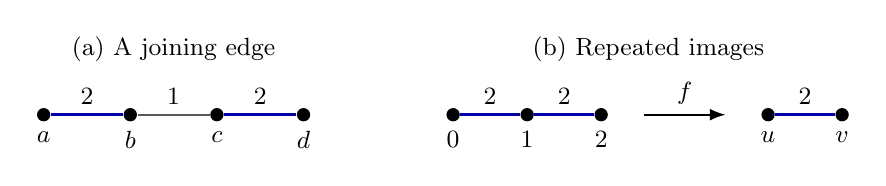
\begin{tikzpicture}[every node/.style={font=\small}]
\node at (1.65,0.83) {(a) A joining edge};
\node[graph vertex,label=below:$a$] (a) at (0,0) {};
\node[graph vertex,label=below:$b$] (b) at (1.1,0) {};
\node[graph vertex,label=below:$c$] (c) at (2.2,0) {};
\node[graph vertex,label=below:$d$] (d) at (3.3,0) {};
\draw[marked edge] (a)--node[above] {$2$} (b);
\draw[unmarked edge] (b)--node[above] {$1$} (c);
\draw[marked edge] (c)--node[above] {$2$} (d);

\begin{scope}[xshift=5.2cm]
\node at (2.48,0.83) {(b) Repeated images};
\node[graph vertex,label=below:$0$] (p0) at (0,0) {};
\node[graph vertex,label=below:$1$] (p1) at (0.94,0) {};
\node[graph vertex,label=below:$2$] (p2) at (1.88,0) {};
\node[graph vertex,label=below:$u$] (u) at (4,0) {};
\node[graph vertex,label=below:$v$] (v) at (4.94,0) {};
\draw[marked edge] (p0)--node[above] {$2$} (p1);
\draw[marked edge] (p1)--node[above] {$2$} (p2);
\draw[-{Latex[length=2mm]},semithick] (2.42,0)--node[above] {$f$} (3.46,0);
\draw[marked edge] (u)--node[above] {$2$} (v);
\end{scope}
\end{tikzpicture}
\caption{The edge $bc$ joins the marked edges in (a).
In (b), $f(0)=f(2)=u$ and $f(1)=v$.}
\label{fig:marked-maps}
\end{figure}

The graph underlying a pattern $F$ has an edge for each pair of
color $1$ or $2$. For the simple-graph calculation we use patterns
in which this graph is connected, the edges of color $2$ form a strong
clique in it, and the pair $\{0,1\}$ has color $2$. We call $(0,1)$
the ordered root. Let $h_F$ be the number of maps that give exactly
the colors of $F$. To see why we use the normalized count
$q_F=\frac{h_F}{2m\Delta^{n-2}}$, fix a spanning tree of the underlying
graph that contains the root edge. Choose the image of $(0,1)$
uniformly from the $2m$ ordered marked edges. Work outwards from the
root edge along the tree. Whenever the image of a position is known,
choose the image of each of its children independently and uniformly
from the $\Delta$ neighbors of that image. Each map counted by $h_F$
occurs with probability $\frac{1}{2m\Delta^{n-2}}$. Hence $q_F$ is the
probability that the sampled map gives the prescribed colors on
\emph{all} pairs of positions.

Fix such a pattern $T$ on $k$ positions. A flag $F$ of type $T$
is one of the patterns just described whose restriction to its first
$k$ positions is $T$. Given a map $f$ that gives the colors of $T$,
let $h_F(f)$ count the maps that give the colors of $F$ and agree
with $f$ on these $k$ positions. For a flag on $n$ positions, extend
a spanning tree of $T$ to a spanning tree of $F$. Starting with the
images fixed by $f$, sample the remaining $n-k$ images along the
tree. The probability of obtaining all the colors of $F$ is now
$\frac{h_F(f)}{\Delta^{n-k}}$. This plays the role of the flag
density for a fixed placement of the labels in
\textbf{Subsection~\ref{subsec:flag-algebra}}.

Take flags $F_i$ and $F_j$ of type $T$, with disjoint sets of positions
outside $T$. An extension of $f$ to $F_i$ and an extension of $f$ to
$F_j$ together define a map on the union of their positions. Its images
specify the colors of the remaining pairs, each with one position
in $F_i$ outside $T$ and one in $F_j$ outside $T$. Let
$\mathcal U_{ij}$ be the set of patterns on the union that agree with
both flags and in which the edges of color $2$ form a strong clique.
Every pair of extensions determines exactly one pattern in
$\mathcal U_{ij}$. Conversely, a map giving the colors of any
$H\in\mathcal U_{ij}$ and extending $f$ restricts to one extension
for each flag. Therefore
\[
 h_{F_i}(f)h_{F_j}(f)=\sum_{H\in\mathcal U_{ij}}h_H(f).
\]
The identity holds even when positions outside $T$ in the two flags
have the same image, since the map records their pair as color $0$.
Thus the formal sum $\sum_{H\in\mathcal U_{ij}}H$ in
\eqref{eq:colored-flag-product} gives an exact product rule for these
counts at every $\Delta$. Freedman, Lov\'asz and Schrijver use the
same multiplication of extension counts for partially labeled
graphs~\cite{FreedmanLovaszSchrijver2007}.

In \textbf{Figure~\ref{fig:flag-union}}, only the color of $\{2,3\}$
remains to be determined. Let $H_a$ be the pattern with color $a$
on that pair. All three choices are possible in the formal product.
When $a=2$, for example, the unmarked edge on $\{0,2\}$ joins the
two disjoint marked edges on $\{0,1\}$ and $\{2,3\}$. For these flags
the sum consists of $H_0,H_1,H_2$.

\begin{figure}[htbp]
\centering
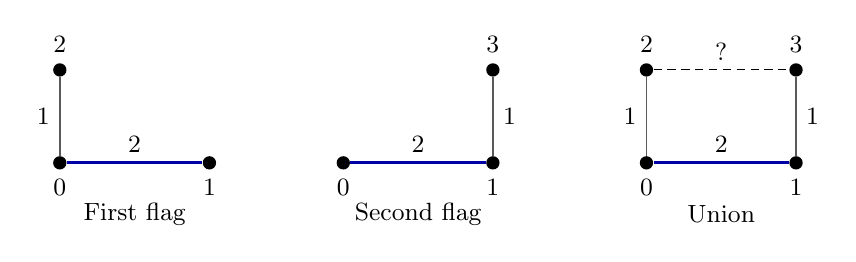
\begin{tikzpicture}[every node/.style={font=\small}]
\node[graph vertex,label=below:$0$] (a0) at (0,0) {};
\node[graph vertex,label=below:$1$] (a1) at (1.9,0) {};
\node[graph vertex,label=above:$2$] (a2) at (0,1.18) {};
\draw[marked edge] (a0)--node[above] {$2$} (a1);
\draw[unmarked edge] (a0)--node[left] {$1$} (a2);
\node at (0.95,-0.65) {First flag};

\begin{scope}[xshift=3.6cm]
\node[graph vertex,label=below:$0$] (b0) at (0,0) {};
\node[graph vertex,label=below:$1$] (b1) at (1.9,0) {};
\node[graph vertex,label=above:$3$] (b3) at (1.9,1.18) {};
\draw[marked edge] (b0)--node[above] {$2$} (b1);
\draw[unmarked edge] (b1)--node[right] {$1$} (b3);
\node at (0.95,-0.65) {Second flag};
\end{scope}

\begin{scope}[xshift=7.45cm]
\node[graph vertex,label=below:$0$] (c0) at (0,0) {};
\node[graph vertex,label=below:$1$] (c1) at (1.9,0) {};
\node[graph vertex,label=above:$2$] (c2) at (0,1.18) {};
\node[graph vertex,label=above:$3$] (c3) at (1.9,1.18) {};
\draw[marked edge] (c0)--node[above] {$2$} (c1);
\draw[unmarked edge] (c0)--node[left] {$1$} (c2);
\draw[unmarked edge] (c1)--node[right] {$1$} (c3);
\draw[densely dashed] (c2)--node[above] {$?$} (c3);
\node at (0.95,-0.65) {Union};
\end{scope}
\end{tikzpicture}
\caption{Two flags with common type on $\{0,1\}$. In their union,
the dashed pair has color $0$, $1$ or $2$. Undrawn pairs have color $0$.}
\label{fig:flag-union}
\end{figure}

The product rule gives inequalities as follows. Fix a list of flags of
type $T$. For the $i$th flag $F_i$, on $n_i$ positions, put
$v_i(f)=\frac{h_{F_i}(f)}{\Delta^{n_i-k}}$. Let $v(f)$ be the column
vector with these entries. The matrix
\[
 \frac{1}{2m\Delta^{k-2}}\sum_f v(f)v(f)^{\mathsf T}
\]
is positive semidefinite, since each summand is an outer product.
The sum ranges over the maps giving the colors of $T$. In its
$(i,j)$ entry the product rule sums the counts of patterns
$H\in\mathcal U_{ij}$ on $n_i+n_j-k$ positions. Each map counted by
$h_H$ has a unique restriction to $T$, so $\sum_f h_H(f)=h_H$.
The three factors in the denominator give
$2m\Delta^{k-2}\Delta^{n_i-k}\Delta^{n_j-k}
=2m\Delta^{n_i+n_j-k-2}$. Thus the entry is
$\sum_{H\in\mathcal U_{ij}}q_H$, as in \eqref{eq:moment-expansion}.
In the example of \textbf{Figure~\ref{fig:flag-union}} it is
$q_{H_0}+q_{H_1}+q_{H_2}$. Consequently each quadratic form of this matrix, evaluated at a fixed
real vector, gives a linear expression in the counts $q_H$ whose
value is nonnegative.

For a multigraph, a map into the simple support records which pairs
of vertices are adjacent. We also have to record how many edges of
the strong clique join each pair. Call an edge of the support
\emph{red} if at least one marked copy joins its endpoints. For each
red edge $uv$, distinguish one marked copy, called the \emph{base
copy}, and let $b_{uv}$ be the number of other marked copies, called
\emph{extra copies}. A pattern can now require an extra copy on one
or more specified edges. If the map sends such an edge to $uv$, there
are $b_{uv}$ choices for that copy. For a fixed map, multiplying
these numbers counts the choices on all specified edges.

For two flags with a common type, first choose the copies required
on the type. The choices on each flag outside the type are then
independent, so the same product rule counts pairs of extensions.
When the type itself requires extra copies, its map $f$ contributes
an outer product multiplied by the number of choices on the type.
This number is nonnegative, and the resulting matrix is again positive
semidefinite. \textbf{Subsection~\ref{sec:weighted-counts}} specifies
the weighted counts used in the multigraph proof.

\subsection{The Uniform Bound for Simple Graphs}\label{subsec:marked-edge-pairs}

We now express $\frac{m}{\Delta^2}$ in terms of the counts $q_F$.
Choose the images of $(0,1)$ and $(2,3)$ independently from the $2m$
ordered marked edges. The two choices may give the same edge. Each
choice determines the images of four positions and hence the colors of
all six pairs. If the two image edges are disjoint, a joining edge
exists because the marked edges form a strong clique. If they share
an endpoint, a position for that endpoint is adjacent in the pattern
to a position on the other edge. Thus the pattern is connected in
either case. Let $\mathcal B$ consist of the connected patterns on
these four positions whose edges of color $2$ form a strong clique
and include $\{0,1\}$ and $\{2,3\}$. Each choice of the two ordered
edges contributes to exactly one $h_F$ with $F\in\mathcal B$, and
every map counted by such an $h_F$ determines the two ordered edges.
Therefore
\[
 \sum_{F\in\mathcal B}h_F=(2m)^2,\qquad
 \frac{1}{2}\sum_{F\in\mathcal B}q_F=\frac{m}{\Delta^2}.
\]

To bound this sum we use the flag inequalities from
\textbf{Subsection~\ref{subsec:adapted-flags}} and the degree
equations. For the latter, fix a position in a pattern and require
one new position to map to a neighbor of its image. Every map of the
old positions has exactly $\Delta$ extensions. Sorting these
extensions by their pair colors gives \eqref{eq:degree-extension}
after normalization. The calculation in
\textbf{Subsection~\ref{sec:simple-proof}} uses the degree equations to
express $\frac{5}{4}-\frac{1}{2}\sum_{F\in\mathcal B}q_F$ as a sum
of nonnegative multiples of individual counts $q_F$ and of quadratic
forms of the positive semidefinite matrices with nonnegative weights. The identity is \eqref{eq:certificate-identity},
with rational coefficients checked in the proof of
\textbf{Lemma~\ref{prop:checked-certificate}}. Its right-hand side
is nonnegative. The identity for the two ordered edges now gives
$m\leq\frac{5}{4}\Delta^2$.

\subsection{From Simple Graphs to Multigraphs}\label{subsec:weighted-sketch}

Let $D$ be a positive integer and let $G$ be a loopless multigraph of
maximum degree at most $D$. Mark the $m>0$ edges of a strong clique.
Keep the subgraph induced by their endpoints. Between vertices joined
by marked edges, keep all the marked copies. Between any other two
adjacent vertices, keep one unmarked edge. Thus each pair of disjoint
marked edges still has a joining edge. Let $s$ be the number of red
edges in the simple support and $b=m-s$ the total number of extra
copies. The $s$ red edges form a strong clique in the simple support,
so the simple-graph bound gives $s\leq\frac{5}{4}D^2$.

The degree of a vertex in the reduced multigraph is its number of
distinct neighbors plus the number of extra copies incident with it.
As shown in \textbf{Subsection~\ref{sec:weighted-counts}}, we may add
unmarked edges and vertices to make the multigraph $D$-regular while
preserving its induced subgraph on the old vertices. Then, for each
vertex $v$, the extension by one incident edge has exactly $D$
choices. A neighbor $u$ joined to $v$ by an unmarked edge contributes
one choice. A neighbor on a red edge $uv$ contributes one choice of
the base copy and $b_{uv}$ choices of an extra copy. Counting these
choices in the weighted patterns gives the degree equations for
multigraphs.

Choose two ordered marked copies as in the simple-graph calculation.
There are $2s$ choices for an ordered base copy and $2b$ for an ordered
extra copy. Thus the numbers of choices using zero, one and two extra
copies are $(2s)^2$, $2(2s)(2b)$ and $(2b)^2$, respectively. Dividing
each count by $4mD^2$ gives the identity
\[
 \frac{s^2}{mD^2}+\frac{2sb}{mD^2}+\frac{b^2}{mD^2}
 =\frac{m}{D^2}.
\]
Each term on the left is a linear combination of the weighted
pattern counts. For example, in the last term each chosen edge of
the support contributes its number of extra copies.

Write $M=\frac{m}{D^2}$, $S=\frac{s}{D^2}$ and $e=\frac{b}{m}$.
Then $S=M(1-e)$. Suppose that $M>\frac{5}{4}$. The weighted flag
inequalities first give upper bounds on both $M$ and $e$. Degree
estimates on induced five-cycles of red edges, together with flag
inequalities in the simple support, give an upper bound on $S$.
The identity $e=1-\frac{S}{M}$ then gives a lower bound on $e$.
With $e$ restricted to this interval, the weighted flag inequalities
give a smaller upper bound on $M$. The successive bounds in the proof
of \textbf{Lemma~\ref{prop:multi-uniform}} yield $M<\frac{5}{4}$,
contradicting our assumption. This proves $m\leq\frac{5}{4}D^2$.
For even $D$, the right-hand side is $f(D)$.

\subsection{The Structure of a Counterexample}\label{subsec:odd-sketch}

Let $D=\Delta(G)$ be odd. If the bound $f(D)$ fails, mark exactly
$m=f(D)+1$ edges of a strong clique and keep the multigraph on their
endpoints as in \textbf{Subsection~\ref{subsec:weighted-sketch}}.
The definition of $f(D)$ gives
\[
 M=\frac{m}{D^2}=\frac{5}{4}-\frac{1}{2D}+\frac{5}{4D^2}.
\]
For $D\geq9$ this value is at least $\frac{98}{81}$, with equality
at $D=9$. If the simple support contained no induced five-cycle with
all five edges red, the flag inequality \eqref{eq:absence-red-cycle} would give
$M<\frac{98}{81}$. Thus the support contains such a cycle, as stated
in \textbf{Lemma~\ref{lem:counterexample-cycle}}. We examine the degrees around
each such cycle to bound $s$, the number of distinct pairs of
endpoints of the $m$ marked edges.

Fix one of these cycles, say $c_0c_1c_2c_3c_4c_0$, and take
indices modulo five. For each $i$, let $U_i$ consist of the vertices
whose only neighbors on the cycle are $c_{i-1}$ and $c_{i+1}$ and
whose edges to both of these vertices are red. In particular,
$c_i\in U_i$. Take $x\in U_0$ and $y\in U_1$. The disjoint red edges
$xc_4$ and $yc_2$ must have a joining edge. The definitions of
$U_0,U_1$ exclude $xc_2$ and $yc_4$, and the induced cycle has no
edge $c_4c_2$. Thus $xy$ is an edge of the support. The same argument
with indices shifted shows that each vertex of $U_i$ is adjacent to
every vertex of $U_{i-1}$ and $U_{i+1}$.

In particular, $c_i$ is joined to at least $|U_{i-1}|+|U_{i+1}|$
distinct vertices in the multigraph. After counting one copy of each
of these edges, at most $D-|U_{i-1}|-|U_{i+1}|$ more edges can be
incident with $c_i$. The sum of these five upper bounds is
$R=5D-2\sum_{i=0}^4|U_i|$. For odd $D\geq11$, the degree count in
\textbf{Subsection~\ref{subsec:exact-large-degree}} shows that $R>\frac{D+1}{2}$ on
every such cycle in a counterexample.

To see how this structural restriction yields an inequality, let
$q_C$ be the number of ordered red induced five-cycles divided by
$2sD^3$. Here an ordered cycle has a specified starting vertex and
direction. Let $L_R$ be the sum of $\frac{R}{D}$ over the same
ordered cycles, divided by the same denominator. The bound on $R$
gives $L_R\geq\frac{q_C}{2}$. One of the flag inequalities for the
simple support in \eqref{eq:support-projection-four} gives
\[
 S+0.45119\left(L_R-\frac{q_C}{2}\right)\leq 1.221800627,
 \qquad\text{where }S=\frac{s}{D^2}.
\]
Its second term on the left is nonnegative. Thus
$S\leq1.221800627$. For odd $D\geq15$, the value of $M$ above
satisfies $M\geq\frac{11}{9}>1.221800627$. It follows that $s<m$,
so some pair of vertices is joined by at least two marked copies.
Moreover, $e=1-\frac{S}{M}$ gives an explicit lower bound on the
fraction of extra copies.

For $D=11,13$, the integer $R$ is odd, and the degree estimates
in \textbf{Subsection~\ref{subsec:exact-large-degree}} give $R\geq9$. Substituting
$L_R\geq\frac{9}{D}q_C$ into the flag inequalities gives $S<M$
in these two cases as well. At $D=9$, the finite simple-graph
bound excludes $s=m$. The remaining degree estimates restrict $e$
further. For each odd $D\geq9$ the weighted flag inequalities then
exclude the prescribed value $M=\frac{f(D)+1}{D^2}$ throughout the
allowed interval for $e$, as detailed in
\textbf{Table~\ref{tab:multi-odd}}. The cases $D=1,3,5,7$ are
settled separately in \textbf{Subsection~\ref{subsec:exact-small-degree}}. This proves
\textbf{Theorem~\ref{thm:multigraph}}.
\section{Comparison with Earlier Work}\label{sec:earlier-work}

\subsection{Earlier Work}

Let $H$ consist of the edges of a nonempty strong clique in $G$ and
their endpoints. Write $\Delta=\Delta(G)$ and $h=\Delta(H)$. Fix an
edge $xy$ of $H$. Every edge of $H$ meets $X=N_G(x)\cup N_G(y)$.
Indeed, $x,y\in X$, and any edge disjoint from $xy$ must have an
endpoint adjacent to $x$ or $y$. Thus $|E(H)|\leq |X|h\leq2\Delta h$.
Faudree, Gy\'arf\'as, Schelp and Tuza~\cite{FGST1990} asked what
would happen if this count came arbitrarily close to $2\Delta^2$.
The set $X$ would have close to $2\Delta$ vertices, and most of them
would have close to $\Delta$ edges of $H$ leading outside $X$, since
an edge inside $X$ is counted at both ends. Consider two such edges
$zu,z'u'$ with distinct $z,z'\in X$ and distinct $u,u'\notin X$.
If none of $zz',zu',z'u$ is present, then $uu'$ must be present.
The authors count these required edges at the outside neighbors of
a fixed $z$, together with the edges from those neighbors back to
$X$. The two counts exceed the available degree when
$|E(H)|>(2-\varepsilon)\Delta^2$ for sufficiently small absolute
$\varepsilon>0$. Hence $|E(H)|\leq(2-\varepsilon)\Delta^2$.

For simple graphs, \'{S}leszy\'{n}ska-Nowak~\cite{SleszynskaNowak2016}
used all the edges at a vertex $v$ with $d_H(v)=h$. At most $\Delta h$
edges of $H$ meet $N_G(v)$. Let $F$ consist of the remaining edges.
For every $a\in N_H(v)$, the set $N_G(a)\cap V(F)$ covers $E(F)$,
since each edge of $F$ must be joined to $va$ and neither endpoint is
adjacent to $v$. A vertex belonging to $j$ of these covers already
has $j$ neighbors outside $V(F)$ and hence has degree at most
$\Delta-j$ in $F$. When $h\geq\frac{3}{4}\Delta$, her count using
these covers gives $|E(F)|\leq\Delta^2-\frac{1}{2}\Delta h$.
Adding the edges meeting $N_G(v)$ gives
$|E(H)|\leq\Delta^2+\frac{1}{2}\Delta h\leq\frac{3}{2}\Delta^2$.
For smaller $h$, the bound $|E(H)|\leq2\Delta h$ already suffices.

Faron and Postle~\cite{FaronPostle2019} kept track of the degree sum
at the two ends of each edge of $H$. Write $\sigma=\sigma_G(H)$ for
the largest of these sums, with both degrees measured in $G$.
They chose $x$ of maximum degree in $H$ and, among its neighbors
in $H$, chose $y$ of largest degree in $H$. Their double counting
argument starts by summing the degrees in $H$ of the vertices in
$N_G(x)\cup N_G(y)$ and subtracting the edges counted twice.
For the second count, consider the edges from outside this union to
vertices adjacent to $x$ but not $y$, and those to vertices adjacent
to $y$ but not $x$. Each set forms a
smaller bipartite subgraph of $H$. In the first subgraph neither
endpoint of an edge is adjacent to $y$. For that edge to have a
joining edge to every edge of $H$ at $y$, each neighbor of $y$ in
$H$ must be adjacent to one of its endpoints. Those neighbors lie outside
the subgraph, so restricting $G$ to the vertices of this subgraph
lowers the endpoint degree sum by at least $d_H(y)$. The second
subgraph gives the corresponding decrease of at least $d_H(x)$.

Combining the two counts, Faron and Postle showed that an estimate
with coefficient $\beta\in[\frac{1}{4},\frac{1}{3}]$ for smaller
bipartite subgraphs of $H$ gives the estimate
$|E(H)|\leq\frac{1+\beta}{4}\sigma^2$ for general $H$.
Here the bipartite estimate is $|E(H')|\leq\beta\sigma_{G'}(H')^2$,
where $H'$ is the smaller bipartite subgraph and $G'=G[V(H')]$.
The edges of $H'$ still form a strong clique in $G'$ because all
their endpoints are retained. At $\beta=\frac{1}{3}$, the coefficient
$\frac{1+\beta}{4}$ is again $\frac{1}{3}$, so induction on $|E(H)|$
gives $|E(H)|\leq\frac{1}{3}\sigma^2\leq\frac{4}{3}\Delta^2$.

Kumar, Mohar and Pragada~\cite{KumarMoharPragada2026} improved the
bipartite estimate in this reduction. Suppose that $H$ is bipartite.
Choose $v$ with $d_H(v)=h$, put $A=N_H(v)$ and let
$B=V(H)\setminus N_G[v]$. For an edge $xy$ of $H[B]$, every
$a\in A$ must be adjacent to $x$ or $y$, since $va$ and $xy$ need
a joining edge. Thus $d_{G[B]}(x)+d_{G[B]}(y)\leq\sigma-h$,
and induction bounds $|E(H[B])|$ by $\beta(\sigma-h)^2$.
The same edges from $A$ to $B$ also enter the count at $A$.
Those outside $H$ use degree at $A$ without contributing to $|E(H)|$.
The authors subtract these edges when counting the edges of $H$
meeting $N_G[v]$. Combining this count with the induction bound
reduces the estimate to an inequality in $h/\sigma$, which they
verify for $\beta=\frac{620}{1987}$. The reduction above and
$\sigma\leq2\Delta$ then give
$|E(H)|\leq(1+\beta)\Delta^2=\frac{2607}{1987}\Delta^2$.

A different question is when a five-cycle must occur and what its
vertices tell us about the rest of the graph. Chung, Gy\'arf\'as,
Tuza and Trotter~\cite{CGTT1990} considered simple graphs in which
the entire edge set is a strong clique. After deleting isolated
vertices, such a graph has no induced subgraph consisting of two
disjoint edges. In the triangle-free, nonbipartite case, a shortest
odd cycle must have length five, since a longer induced cycle contains
two edges with no joining edge. Every vertex has exactly two neighbors
on the five-cycle. Vertices with the same two neighbors form one of
five independent sets. Every edge between successive sets is present,
so if their sizes in cyclic
order are $a_0,\ldots,a_4$, then the edge count is
$\sum_{i=0}^4 a_i a_{i+1}$ and $a_{i-1}+a_{i+1}\leq\Delta$ for
each $i$, with indices modulo five. Maximizing this sum gives
$f(\Delta)$. In the bipartite case each part contains a vertex
adjacent to the whole other part, so there are at most $\Delta^2$
edges. If there is a triangle, they find a maximum clique such that
every vertex outside it has a neighbor in it. Grouping the outside
vertices according to their neighbors in this clique and counting
the edges gives fewer than $f(\Delta)$ edges.

Cames van Batenburg, Kang and Pirot~\cite{CamesKangPirot2020}
allowed $H$ to be a proper submultigraph and assumed that $G$ has
no five-cycle. Again take $v$ with $d_H(v)=h$. Consider an edge
$xy$ of $H$ with both ends outside $N_G[v]$. Each $a\in N_H(v)$
must be adjacent to $x$ or $y$. If distinct $a,b\in N_H(v)$
were adjacent to $x$ and $y$, respectively, then $vaxybv$ would
be a five-cycle. Thus, when $|N_H(v)|\geq2$, one endpoint of $xy$
is adjacent to every vertex of $N_H(v)$. The authors count the
edges at these endpoints, then subtract the degree already used by
their neighbors in $N_H(v)$ when counting the remaining clique edges.
Together with the case $|N_H(v)|=1$, this gives
$|E(H)|\leq h(\sigma-h)\leq\frac{1}{4}\sigma^2\leq\Delta^2$.
Consequently a larger strong clique forces some five-cycle in $G$.
For our argument we need an induced five-cycle in the simple support
of $G$ with an edge of $H$ on each of its five pairs of endpoints.

\subsection{Highlights of the Proof}\label{subsec:method-highlights}

The main idea is to use the structure of a counterexample at odd
maximum degree to derive an inequality on edge multiplicities that
contradicts the weighted flag inequalities. Suppose that $G$ has odd
maximum degree $D$ and contains a strong clique of $m=f(D)+1$ marked edges.
For $D\geq9$, \textbf{Lemma~\ref{lem:counterexample-cycle}} gives an
induced five-cycle in the simple support of $G$. Each edge of the cycle
has the same endpoints as a marked edge of $G$. This allows us to
use the five sets suggested by the blow-ups of $C_5$ in the work
of Chung, Gy\'arf\'as, Tuza and Trotter~\cite{CGTT1990}, even when
the host has unmarked edges and parallel edges.

For each such cycle $C$, let $U_0,\ldots,U_4$ be the sets defined
in \textbf{Subsection~\ref{subsec:odd-sketch}}. All edges between
$U_i$ and $U_{i+1}$ are present in the simple support, with indices
taken modulo five. Thus at the $i$th cycle vertex at least
$|U_{i-1}|+|U_{i+1}|$ of its incident edges are already accounted for.
Summing over the five vertices leaves at most
$R(C)=5D-2\sum_{i=0}^4|U_i|$ further incidences.
When $D\geq11$, counting the marked edges in and outside these
sets shows that $R(C)\leq\frac{D+1}{2}$ would give $m\leq f(D)$.
Consequently $R(C)>\frac{D+1}{2}$ on every such cycle of a
counterexample. This use of restrictions on small induced subgraphs
to sharpen a flag bound is related to the stability arguments of
Pikhurko, Slia\v{c}an and Tyros~\cite{PikhurkoSliacanTyros2019}.

Let $s$ be the number of distinct pairs of vertices joined by
marked edges. Summing the lower bound on $R(C)$ over the cycles
and substituting it into the flag inequalities for the simple
support gives an upper bound on $s$. For example, for odd
$D\geq15$ we obtain
\[
  \frac{s}{D^2}\leq 1.221800627
  <\frac{11}{9}\leq\frac{m}{D^2}.
\]
Once one marked edge has been counted on each of the $s$ pairs,
the other $m-s$ marked edges are parallel copies. An upper bound
on $s$ is therefore a lower bound on the fraction $\frac{m-s}{m}$
of such copies. At $D=15$, for instance, the degree estimates give
$R(C)\geq11$ on every induced red five-cycle. Using this bound in the
inequalities for the simple support, and counting the extra copies at
their endpoints, gives $0.007\leq\frac{m-s}{m}\leq0.365$
in \textbf{Section~\ref{sec:exact}}.
With these restrictions, the weighted flag inequalities in the
$D=15$ row of \textbf{Table~\ref{tab:multi-odd}} give
$\frac{m}{D^2}<0.827$. Yet $m=f(15)+1=275$ requires
$\frac{m}{D^2}=\frac{11}{9}$. The other rows give the contradiction
for the remaining odd $D\geq9$.
\section{Auxiliary Lemmas}\label{sec:auxiliary}

We use a regular supergraph to count the ways to extend a map by one
vertex. We refine the regularization lemma of Davey et
al.~\cite{DaveyEtAlStrong2026} for simple graphs by extending it to
loopless multigraphs. The construction preserves the multiplicities
of the original edges and gives every new edge multiplicity one.

\begin{lemma}\label{lem:regularization}
Let $D\geq1$ be an integer and let $G$ be a finite loopless multigraph
with $\Delta(G)\leq D$. There is a finite $D$-regular loopless multigraph
$\widehat G$ containing $G$ as an induced subgraph such that every
edge of $\widehat G$ outside $G$ has multiplicity one. In particular, $\widehat G$ is simple
if $G$ is simple.
\end{lemma}

\begin{proof}
We must add $D-d_G(v)$ incidences at each vertex $v$. Their total
is $D|V(G)|-2|E(G)|$. If it is odd, then $D$ is odd, so adjoining one
isolated vertex makes the total even. Form a list containing $D-d(v)$
occurrences of each vertex $v$ of the resulting graph, where $d(v)$ is
its current degree. Partition the list into pairs. For a pair $(u,v)$,
take a new copy of $K_{D+1}$, delete an edge $xy$, and add the edges
$ux$ and $vy$. Use a different copy for each pair. This adds two
distinct edges even when $u=v$. Both $x$ and $y$ regain degree $D$,
and every occurrence in the list adds one incidence at the
corresponding vertex. Thus all degrees are $D$. Each added edge has
multiplicity one and at least one new endpoint, so the original
vertices induce $G$.
\end{proof}

A strong clique in $G$ is also a strong clique in $\widehat G$, since
every adjacency between endpoints of its edges is preserved. In the
counting arguments we mark only the edges of the chosen clique, so
all edges added in the construction are unmarked.

Vector inequalities are coordinatewise. For symmetric matrices $X$
and $Y$ of the same size, $\tr(XY)=\sum_{i,j}X_{ij}Y_{ij}$.

In the simple-graph calculation we will express the size of a strong
clique, divided by the square of the maximum degree, as a linear
function of the pattern counts. The calculation uses a system with $N=23{,}789$ coordinates, $3{,}516$ linear equations and
$57$ positive semidefinite matrix constraints. Write $Aq=b$ for the
linear equations and $o^{\mathsf T}q$ for the objective, where
$A\in\mathbb Q^{3516\times N}$, $b\in\mathbb Q^{3516}$ and
$o\in\mathbb Q^N$. For each $\ell\in[57]$, let
$K_\ell,D_{\ell1},\ldots,D_{\ell N}$ be symmetric rational matrices of
the same size. The $\ell$th matrix constraint is $M_\ell(q)\succeq0$,
where
\begin{equation}\label{eq:intro-affine-gram}
 M_\ell(q)=K_\ell+\sum_{j=1}^N q_jD_{\ell j}.
\end{equation}
The matrices and vectors are specified in \textbf{Appendix~\ref{app:data-specification}}.
For a symmetric matrix
$Q$ of the same size as $K_\ell$, define
$D_\ell^*(Q)\in\mathbb R^N$ by
\begin{equation}\label{eq:intro-trace-adjoint}
 (D_\ell^*(Q))_j=\tr(QD_{\ell j})\qquad(j\in[N]).
\end{equation}

\begin{lemma}\label{prop:certificate-principle}
Let $o\in\mathbb Q^N$ be an objective vector and
$\lambda\in\mathbb Q^{3516}$. For each $\ell\in[57]$, let $Q_\ell$
be a matrix of the same size as $K_\ell$ expressible as a finite
nonnegative rational linear combination of outer products
$ww^{\mathsf T}$ of rational vectors. Set
\begin{align}
 &r=A^{\mathsf T}\lambda-\sum_{\ell=1}^{57}D_\ell^*(Q_\ell)-o,
 \label{eq:residual}\\
 &C=b^{\mathsf T}\lambda+\sum_{\ell=1}^{57}\tr(Q_\ell K_\ell).
 \label{eq:dual-value}
\end{align}
We call $r$ the residual vector. If $r\geq0$, then every $q\in\mathbb R^N$ with $q\geq0$, $Aq=b$ and
$M_\ell(q)\succeq0$ for all $\ell\in[57]$ satisfies $o^{\mathsf T}q\leq C$.
If $q\in[0,1]^N$ satisfies the same equations and matrix constraints,
then $o^{\mathsf T}q\leq C-\sum_{j:r_j<0}r_j$, for any residual $r$.
\end{lemma}

\begin{proof}
By \eqref{eq:intro-affine-gram} and
\eqref{eq:intro-trace-adjoint}, each trace
$\tr(Q_\ell M_\ell(q))$ equals
$\tr(Q_\ell K_\ell)+D_\ell^*(Q_\ell)^{\mathsf T}q$.
Adding the scalar product of $r$ in \eqref{eq:residual} with $q$
cancels the terms involving $D_\ell^*(Q_\ell)$. Since $Aq=b$,
we have $\lambda^{\mathsf T}Aq=b^{\mathsf T}\lambda$, so
the definition of $C$ in \eqref{eq:dual-value} gives
\begin{equation}\label{eq:certificate-identity}
 C-o^{\mathsf T}q
 =\sum_{\ell=1}^{57}\tr\bigl(Q_\ell M_\ell(q)\bigr)
  +\sum_{j=1}^N r_jq_j.
\end{equation}
Write $Q_\ell=\sum_a\alpha_{\ell a}w_{\ell a}w_{\ell a}^{\mathsf T}$,
where each $\alpha_{\ell a}$ is nonnegative. Then
\[
 \tr\bigl(Q_\ell M_\ell(q)\bigr)=
 \sum_a\alpha_{\ell a}w_{\ell a}^{\mathsf T}M_\ell(q)w_{\ell a}\geq0
\]
because $M_\ell(q)$ is positive semidefinite. If $r\geq0$ and $q\geq0$,
the second sum in \eqref{eq:certificate-identity} is nonnegative.
For $0\leq q_j\leq1$, we have $r_jq_j\geq0$ if $r_j\geq0$ and
$r_jq_j\geq r_j$ if $r_j<0$. Thus the second sum is at least
$\sum_{j:r_j<0}r_j$ in that case.
\end{proof}
\section{Proof of the Bound \texorpdfstring{$\frac{5}{4}\Delta^2$}{5 Delta squared / 4}}\label{sec:uniform}

Let $G$ be a finite loopless multigraph with maximum degree $\Delta$.
We prove that $\omega(L(G)^2)\leq\frac{5}{4}\Delta^2$. We first
prove the bound for simple graphs. To extend it to multigraphs, we
count how many edges of a given strong clique join each pair of
adjacent vertices.

\subsection{The Bound \texorpdfstring{$\frac{5}{4}\Delta^2$}{5 Delta squared / 4} in Simple Graphs}
\label{sec:simple-proof}\label{sec:finite-model}\label{sec:identities}\label{sec:finite-instance}
\label{subsubsec:conditional-extension-counts}

By \textbf{Lemma~\ref{lem:regularization}}, a nonempty strong clique
in a simple graph of maximum degree $\Delta$ remains a strong clique
in a $\Delta$-regular simple graph. Let $G$ be this regular graph and
mark the set $S$ of edges in the given clique. We retain the other
edges of $G$, which may join the endpoints of disjoint marked edges.
The symmetric function
$c_G\colon V(G)\times V(G)\to\{0,1,2\}$ is given by
\[
 c_G(u,v)=
 \begin{cases}
  2,&uv\in S,\\
  1,&uv\in E(G)\setminus S,\\
  0,&u=v\text{ or }uv\notin E(G).
 \end{cases}
\]

\begin{defn}\label{def:patterns}
For an integer $n\geq2$, put $P_n=\{0,\ldots,n-1\}$. A \emph{pattern}
$F$ of order $n$ assigns a color $c_F(i,j)\in\{0,1,2\}$ to each pair
$ij=\{i,j\}$ of distinct positions in $P_n$, with $c_F(0,1)=2$. We
call $(0,1)$ the ordered root. The underlying graph $H$ of $F$ has
vertex set $P_n$ and edge set consisting of the pairs of color $1$
or $2$. We call $F$ \emph{connected} if $H$ is connected and
\emph{admissible} if the pairs of color $2$ form a clique in $L(H)^2$.
Equivalently, for every two disjoint pairs of color $2$, some pair
with one position in each has color $1$ or $2$.
Let $\mathcal F_n$ be the set of connected admissible patterns of order $n$.
\end{defn}

\begin{defn}\label{def:color-preserving-maps}
Let $F$ be a pattern of order $n$, and let $G$ be a finite simple graph
with marked set $S\subseteq E(G)$. A \emph{color-preserving map} from $F$
to $G$ is a map $f\colon P_n\to V(G)$ such that
$c_F(i,j)=c_G(f(i),f(j))$ for all distinct $i,j\in P_n$.
For fixed $G$ and $S$, let $h_F$ be the number of color-preserving maps
from $F$ to $G$.
\end{defn}

Distinct positions may map to the same vertex, in which case their
pair has color $0$.

\begin{lemma}\label{lem:pullback}
Let $G$ be a finite simple graph, let $S\subseteq E(G)$ be a clique
in $L(G)^2$, and let $n\geq 2$. Every map $f\colon P_n\to V(G)$ with
$c_G(f(0),f(1))=2$ gives an admissible pattern $F$ by setting
$c_F(i,j)=c_G(f(i),f(j))$ for all distinct $i,j\in P_n$.
\end{lemma}

\begin{proof}
Consider disjoint pairs $ij$ and $k\ell$ of color $2$ in $F$. Their
images are edges of $S$. If the image edges are disjoint, some
endpoint of one is adjacent to an endpoint of the other since $S$
is a clique in $L(G)^2$. The corresponding pair of positions has
color $1$ or $2$.

If the image edges have a common endpoint, we may name the positions
so that $f(i)=f(k)$. The pair $jk$ then maps to the marked edge
$f(j)f(i)$ and has color $2$. The same reasoning applies when the
image edges are equal.
\end{proof}

Let $G$ be a finite simple $\Delta$-regular graph with $\Delta>0$,
and let $S\subseteq E(G)$ be a nonempty clique in $L(G)^2$ of size $m$.
For $F\in\mathcal F_n$, define
\begin{equation}\label{eq:q-definition}
 q_F=\frac{h_F}{2m\Delta^{n-2}}.
\end{equation}
The factor $2m$ counts the possible images of the ordered root.
For the two-position pattern $E_\star$ with its unique pair marked,
we have $h_{E_\star}=2m$ and hence $q_{E_\star}=1$.

Two patterns $F,F'\in\mathcal F_n$ are equivalent if there is a
permutation $\pi$ of $P_n$ with
$c_F(i,j)=c_{F'}(\pi(i),\pi(j))$ for every pair $ij$ of distinct
positions. The preimage of $\{0,1\}$ under $\pi$ may be any pair of
color $2$ in $F$, with either ordering of its two positions. These
are isomorphism classes of the colored patterns with the root allowed
to move. We call them orbits, as in the data files.

For $k\geq2$, $F\in\mathcal F_k$ and $u\in P_k$, let
$\mathcal E(F,u)$ be the set of admissible patterns on $P_{k+1}$ whose
restriction to $P_k$ is $F$ and whose pair $uk$ has color $1$ or $2$.
Each such pattern is connected because its restriction to $P_k$ is
connected and the new position $k$ is adjacent to $u$.

\begin{lemma}\label{lem:coordinates}\label{lem:degree}
Suppose that $G$ is $\Delta$-regular and that its $m>0$ marked edges
form a strong clique. For every $k\geq2$ and $F\in\mathcal F_k$,
$q_F\in[0,1]$ and $q_{F'}=q_F$ for every $F'$ in the orbit of $F$.
For each $u\in P_k$,
\begin{equation}\label{eq:degree-extension}
 \sum_{F'\in\mathcal E(F,u)}q_{F'}=q_F.
\end{equation}
\end{lemma}

\begin{proof}
Since $F$ is connected, its underlying graph has a spanning tree
containing the root edge. Choose the image of the ordered root in
$2m$ ways. Then assign images to the remaining positions in order of
increasing distance from $\{0,1\}$ in the tree, so that each new
position has a tree neighbor whose image is already chosen. The pair
joining them has color $1$ or $2$, so the new image has at most
$\Delta$ choices. Thus $0\leq h_F\leq 2m\Delta^{n-2}$, and
$q_F\in[0,1]$ by \eqref{eq:q-definition}.

If $\pi$ is a permutation of $P_n$ with
$c_F(i,j)=c_{F'}(\pi(i),\pi(j))$ for all distinct $i,j$, then
$f\mapsto f\circ\pi$ maps the color-preserving maps of $F'$ to those
of $F$. Precomposing with $\pi^{-1}$ gives the inverse, so
$h_F=h_{F'}$. The two counts have the same denominator in
\eqref{eq:q-definition}, which gives $q_F=q_{F'}$.

Fix a color-preserving map $f$ of $F$. The image of $k$ can be any
of the $\Delta$ neighbors of $f(u)$, including neighbors already
used by $f$. Each choice determines the colors of all pairs involving
$k$ and therefore a unique extension pattern in $\mathcal E(F,u)$.
Admissibility follows from \textbf{Lemma~\ref{lem:pullback}}.
Conversely, a map counted by $h_{F'}$ for $F'\in\mathcal E(F,u)$
restricts to a color-preserving map of $F$ and sends $k$ to a neighbor
of the image of $u$. Thus
$\sum_{F'\in\mathcal E(F,u)}h_{F'}=\Delta h_F$.
Dividing by $2m\Delta^{k-1}$ gives \eqref{eq:degree-extension}.
\end{proof}

Index the $N=23{,}789$ relabeling orbits in
$\bigcup_{n=3}^6\mathcal F_n$ as in \textbf{Appendix~\ref{app:pattern-indices}}.
For each $j\in[N]$, set $q_j=q_F$ for any $F$ in orbit $j$.
We treat $q_{E_\star}=1$ as a constant. When we collect the terms of a
sum over labeled patterns by orbit, each labeled pattern contributes
once to its orbit coordinate.

The degree equations in $Aq=b$ are the identities in
\eqref{eq:degree-extension} written in the orbit coordinates.
In the row for $(F,u)$, each $F'\in\mathcal E(F,u)$ contributes
one to the column indexed by its orbit. If $F=E_\star$, the right
side of \eqref{eq:degree-extension} is $1$. Otherwise we subtract
one from the column indexed by the orbit of $F$ and set the right
side to $0$.

The pairs $(F,u)$ used for the degree equations are specified
in \textbf{Appendix~\ref{app:flag-lists}}, with $F$ of order $2$, $3$,
$4$ or $5$. At order $5$, we use one pattern from each orbit and
take every position of that pattern in turn as $u$. The resulting
$3{,}516$ equations form the system
\begin{equation}\label{eq:linear-system}
 Aq=b.
\end{equation}
For example, the first row, for $F=E_\star$ and $u=1$, is
$q_1+q_2+q_3+2q_4+q_5=1$. The two extensions with color pairs
$(c_{F'}(0,2),c_{F'}(1,2))=(1,2)$ and $(2,1)$ contribute to
the same orbit, giving the coefficient of $q_4$.

A \emph{type} of order $k$ is a pattern $T\in\mathcal F_k$.
A \emph{flag of type $T$} is a pattern in $\mathcal F_n$, for some
$n\geq k$, whose restriction to $P_k$ is $T$. The positions of the
flag remain labeled when counting extensions. Let
$\mathcal L=(F_1,\ldots,F_s)$ be a list of flags of type $T$ of
orders $n_1,\ldots,n_s$, respectively. For a color-preserving map
$f$ of $T$ into $G$ and any flag $F$ of type $T$, let $h_F(f)$ be
the number of color-preserving maps from $F$ to $G$ that extend
$f$. For each $i\in[s]$, put $v_i(f)=\frac{h_{F_i}(f)}{\Delta^{n_i-k}}$.
Let $v(f)$ be the column vector with entries $v_i(f)$. Define the
\emph{moment matrix} for $T$ and $\mathcal L$ by
\begin{equation}\label{eq:moment-definition}
 M(T,\mathcal L)=\frac{1}{2m\Delta^{k-2}}
       \sum_{f:T\to G}v(f)v(f)^{\mathsf T}.
\end{equation}
The sum runs over all color-preserving maps of $T$ into $G$. If a
flag $F_i$ equals $T$, then $v_i(f)=1$ for each such map.

\begin{lemma}\label{lem:moment}
For any finite list $\mathcal L$ of flags of type $T\in\mathcal F_k$,
the moment matrix $M(T,\mathcal L)$ is positive semidefinite.
If $n_i+n_j-k\leq6$ for all $i,j\in[s]$, each entry is a nonnegative
integer linear combination of the coordinates of $q$ and the
constant $q_{E_\star}=1$.
\end{lemma}

\begin{proof}
By \eqref{eq:moment-definition}, for every $x\in\mathbb R^s$,
$x^{\mathsf T}M(T,\mathcal L)x$ is the sum of the squares
$(x^{\mathsf T}v(f))^2$ divided by $2m\Delta^{k-2}$, so it is
nonnegative.

To compute entry $(i,j)$, put $n=n_i+n_j-k$. In $P_n$, identify each position $r$ of $F_i$ with $r\in P_{n_i}$.
Identify position $r$ of $F_j$ with $r$ if $r<k$ and with $n_i+r-k$
otherwise. The flags agree on their intersection
$P_k$. The unspecified pairs have one position in
$P_{n_i}\setminus P_k$ and the other in $P_n\setminus P_{n_i}$.
Let $\mathcal U_{ij}$ be the set of admissible completions of the
colors of these pairs. Each completed pattern is connected because
the flags are connected and share the type. We write the product of
the two colored flags as the formal sum
\begin{equation}\label{eq:colored-flag-product}
 F_i\star_T F_j=\sum_{H\in\mathcal U_{ij}}H.
\end{equation}
The positions are labeled, so each admissible assignment of
the unspecified colors contributes one summand.

Fix a color-preserving map $f$ of $T$. A pair of extensions of $f$
to $F_i$ and $F_j$ gives a unique map on $P_n$, since the extensions
agree on $P_k$. The images of distinct positions may coincide,
including positions from different flags. Evaluating $c_G$ on the
images of each unspecified pair determines its color. The resulting
pattern belongs to $\mathcal U_{ij}$ by
\textbf{Lemma~\ref{lem:pullback}}. Conversely, a map counted by
$h_H(f)$ for $H\in\mathcal U_{ij}$ restricts to an extension of $f$
to each of the two flags. Counting these pairs and dividing by
$\Delta^{(n_i-k)+(n_j-k)}=\Delta^{n-k}$ gives
\begin{equation}\label{eq:colored-flag-evaluation}
 v_i(f)v_j(f)=\frac{\displaystyle\sum_{H\in\mathcal U_{ij}}h_H(f)}
                         {\Delta^{n-k}}.
\end{equation}
Thus the product in \eqref{eq:colored-flag-product} expresses the
product of the two normalized extension counts exactly.

Substitute \eqref{eq:colored-flag-evaluation} into
\eqref{eq:moment-definition}. Summing $h_H(f)$ over all maps
$f$ of $T$ gives $h_H$, since each color-preserving map of $H$
has a unique restriction to $T$. The total power of $\Delta$ in
the denominator is $(k-2)+(n-k)=n-2$. Hence
\eqref{eq:q-definition} gives
\begin{equation}\label{eq:moment-expansion}
 \bigl(M(T,\mathcal L)\bigr)_{ij}
 =\frac{\displaystyle\sum_{H\in\mathcal U_{ij}}h_H}{2m\Delta^{n-2}}
 =\sum_{H\in\mathcal U_{ij}}q_H.
\end{equation}
For the flags in \textbf{Figure~\ref{fig:flag-union}}, let $H_a$ be
the completion that assigns color $a$ to the pair $23$, for
$a\in\{0,1,2\}$. All three completions are admissible. In particular,
when $23$ has color $2$, the pairs $02$ and $13$ of color $1$ join
the marked pairs $01$ and $23$. The product in
\eqref{eq:colored-flag-product} is therefore $H_0+H_1+H_2$.
Both flags occur in the list of nine flags for the marked
two-position type in \textbf{Table~\ref{tab:blocks}}. Their product
gives the entry $q_{H_0}+q_{H_1}+q_{H_2}$ of the corresponding
moment matrix.

If $n=2$, the union is $E_\star$ and contributes the constant $1$.
If $3\leq n\leq6$, each summand contributes to the coordinate of
its relabeling orbit.
\end{proof}

In \eqref{eq:moment-expansion}, the coefficient of an orbit coordinate
counts the labeled completions in that orbit. If two flags differ
only by a permutation of their positions outside the type, that
permutation gives a bijection between their extensions of each
type map. We therefore use one representative of each class of
flags under permutations fixing the type positions.

The system uses $57$ pairs $(T_\ell,\mathcal L_\ell)$, with types of
order $2$, $3$ or $4$. The flag orders in
\textbf{Table~\ref{tab:blocks}} ensure $n_i+n_j-k\leq6$ for every
pair of flags in the same list. For the graph counts, we set
$M_\ell(q)=M(T_\ell,\mathcal L_\ell)$. To write these matrices as in
\eqref{eq:intro-affine-gram}, let $(D_{\ell j})_{ab}$ count the labeled
completions in $\mathcal U_{ab}$ that belong to orbit $j$, where
$\mathcal U_{ab}$ is taken for the list $\mathcal L_\ell$.
A union of order $2$ occurs only when both flags equal the type
$E_\star$. This gives a $1$ at the first diagonal entry of $K_\ell$
in each of the two lists with this type, and every other entry of
every $K_\ell$ is $0$. By \textbf{Lemma~\ref{lem:moment}},
\begin{equation}\label{eq:positive-moments}
 M_\ell(q)\succeq0\qquad(\ell\in[57]).
\end{equation}

To express $\frac{m}{\Delta^2}$ in terms of $q$, we choose the
images of $(0,1)$ and $(2,3)$ independently from the $2m$ ordered
marked edges. Let $\mathcal B\subseteq\mathcal F_4$ consist of the
patterns in which both $01$ and $23$ have color $2$. For $j\in[N]$,
let $o_j$ be half the number of patterns in $\mathcal B$ belonging
to orbit $j$. Then
\begin{equation}\label{eq:objective-vector}
 o^{\mathsf T}q=\frac{1}{2}\sum_{F\in\mathcal B}q_F.
\end{equation}

\begin{lemma}\label{lem:finite-encoding}\label{lem:objective}
Let $G$ be a finite simple graph of maximum degree $\Delta>0$, and
let $S\subseteq E(G)$ be a strong clique of size $m>0$. For the system
specified in \textbf{Appendix~\ref{app:data-specification}}, there exists
$q\in[0,1]^N$ such that $Aq=b$, $M_\ell(q)\succeq0$ for all
$\ell\in[57]$, and
\begin{equation}\label{eq:objective-value}
 o^{\mathsf T}q=\frac{m}{\Delta^2}.
\end{equation}
\end{lemma}

\begin{proof}
Apply \textbf{Lemma~\ref{lem:regularization}} to $G$ with $D=\Delta$
and mark the $m$ edges of $S$ in the regular supergraph. Form $q$
from the counts in \eqref{eq:q-definition}. By
\textbf{Lemma~\ref{lem:coordinates}}, these counts lie in $[0,1]$
and depend only on their orbits. Equations \eqref{eq:linear-system}
and \eqref{eq:positive-moments} give $Aq=b$ and $M_\ell(q)\succeq0$
for all $\ell\in[57]$. It remains to evaluate $o^{\mathsf T}q$.

There are $(2m)^2$ choices for the two ordered marked images.
Each choice specifies a map of the four positions and therefore
an admissible pattern by \textbf{Lemma~\ref{lem:pullback}}.
Admissibility guarantees a pair of color $1$ or $2$ joining the
two marked pairs of positions. Thus the pattern is connected,
so the choice contributes to exactly one pattern in $\mathcal B$.
Conversely, a map counted by $h_F$ for $F\in\mathcal B$ sends both
pairs to ordered marked edges. Hence $\sum_{F\in\mathcal B}h_F=(2m)^2$.
Using this count in \eqref{eq:q-definition} and
\eqref{eq:objective-vector} gives
\[
 o^{\mathsf T}q
 =\frac{(2m)^2}{2\cdot2m\Delta^2}
 =\frac{m}{\Delta^2}.
\]
\end{proof}

It remains to bound the objective $o^{\mathsf T}q$. We give integer
coefficients for the bound in \textbf{Lemma~\ref{prop:certificate-principle}}
and verify them against the equations and flag products above.

The file \path{reproducibility/data/compact_certificate.json} stores
the vector $L\in\mathbb Z^{3516}$ of degree multiplier numerators.
For each block $\ell\in[57]$, it also gives a list of pairs
$(w_{\ell a},z_{\ell a})$ with $w_{\ell a}\in\mathbb Z_{\geq0}$ and
$z_{\ell a}\in\mathbb Z^{s_\ell}$, where $s_\ell$ is the number of
flags in $\mathcal L_\ell$. These pairs represent the weights
$\frac{w_{\ell a}}{24}$ and vectors $\frac{z_{\ell a}}{10{,}000}$
in a decomposition of $Q_\ell$. We use the common
denominator $\Lambda=24\cdot10{,}000^2=2{,}400{,}000{,}000$ and set
\begin{equation}\label{eq:integral-Q}
 B_\ell=\sum_a w_{\ell a}z_{\ell a}z_{\ell a}^{\mathsf T},
 \qquad Q_\ell=\frac{B_\ell}{\Lambda},
 \qquad \lambda=\frac{L}{\Lambda}.
\end{equation}
There are $4{,}110$ pairs with positive weight across the $57$ blocks.
The representation in \eqref{eq:integral-Q} shows that each $Q_\ell$
is positive semidefinite.

\begin{lemma}\label{prop:checked-certificate}\label{prop:quadratic-bound}\label{lem:rational-witness}
The numerators $L$ and $B_\ell$ in \eqref{eq:integral-Q} satisfy
\begin{align}
 &\rho=A^{\mathsf T}L-\sum_{\ell=1}^{57}D_\ell^*(B_\ell)
                  -\Lambda o\geq0,\label{eq:integer-residual}\\
 &b^{\mathsf T}L+\sum_{\ell=1}^{57}\tr(B_\ell K_\ell)
     =3{,}000{,}000{,}000=\frac{5}{4}\Lambda.
       \label{eq:integer-constant}
\end{align}
Consequently, every finite simple graph $G$ satisfies
$\omega(L(G)^2)\leq\frac{5}{4}\Delta(G)^2$.
\end{lemma}

\begin{proof}
The exact checks in \textbf{Appendix~\ref{app:reproduction}} verify the
degree and moment coefficients against \eqref{eq:degree-extension}
and \eqref{eq:moment-expansion}. With these coefficients, the
residual in \eqref{eq:integer-residual} has $23{,}590$ positive entries
and $199$ zero entries, and the constant in \eqref{eq:integer-constant}
is $3{,}000{,}000{,}000$. Thus $r=\frac{\rho}{\Lambda}\geq0$ and
$C=\frac{5}{4}$ for the multipliers in \eqref{eq:integral-Q}.
If $G$ has an edge, let $m$ be the size of a maximum clique in $L(G)^2$.
For the vector $q$ given by \textbf{Lemma~\ref{lem:finite-encoding}},
\textbf{Lemma~\ref{prop:certificate-principle}} now gives
$o^{\mathsf T}q\leq\frac{5}{4}$.
Since $o^{\mathsf T}q=\frac{m}{\Delta(G)^2}$ by \eqref{eq:objective-value},
we obtain $m\leq\frac{5}{4}\Delta(G)^2$.
If $G$ has no edges, the clique number is zero.
\end{proof}

We next record two consequences of the simple-graph count that we will
use in the proof for multigraphs. The first finds a marked induced
five-cycle when the clique is large enough. The second bounds the
degrees available around that cycle.

Let $G$ be a simple graph with maximum degree at most a positive
integer $D$, and let $m>0$ of its edges form a strong clique.
Mark these $m$ edges. Write $t=\frac{D}{2}$ and
$\mu=\frac{5}{4} D^2-m$. By \textbf{Lemma~\ref{prop:quadratic-bound}},
$\mu\geq0$. When $D$ is odd, $f(D)=5t^2-t+\frac{1}{4}$. A counterexample
with $m>f(D)$ therefore satisfies
\begin{equation}\label{eq:odd-counterexample}
 \mu\leq t-\frac{5}{4}.
\end{equation}

By \textbf{Lemma~\ref{lem:regularization}}, there is a $D$-regular
simple graph $\widehat G$ containing $G$ as an induced subgraph.
Only the original clique edges are marked. In particular every vertex
incident with a marked edge belongs to $G$.
\textbf{Lemma~\ref{lem:finite-encoding}} supplies the normalized
counts for $\widehat G$.

A marked induced five-cycle is an induced cycle of length five in
$\widehat G$ whose five edges are marked. Let $q_C$ be the normalized
count for the pattern with marked cycle $0,1,2,3,4,0$ and root $01$.
Every color-preserving map of this pattern is injective. Adjacent
positions have different images, and given two nonadjacent positions,
there is a third position adjacent to exactly one of them.
In the balanced blow-up with $b$ vertices in each part and all
edges marked, there are $10b^5$ such maps, from the ten cyclic
orderings and the choice of one vertex per part. Hence
$q_C=\frac{10b^5}{2(5b^2)(2b)^3}=\frac{1}{8}$ in that example.

Fix an ordered image $c_0,\ldots,c_4$ of the cycle, taking indices
modulo five. Let $U_i$ consist of the vertices whose neighbors on
the cycle are exactly $c_{i-1},c_{i+1}$ and whose edges to both
cycle vertices are marked. The sets $U_i$ are pairwise disjoint,
contain $c_i$ in $U_i$, and lie in $V(G)$ since every vertex in
them is incident with a marked edge.
\textbf{Figure~\ref{fig:odd-cycle-parts}} illustrates $U_0$. Define
\begin{equation}\label{eq:odd-core-defs}
 a_i=|U_i|,\qquad B=\bigcup_{i=0}^4 U_i,\qquad
 s_i=D-a_{i-1}-a_{i+1},\qquad R=\sum_{i=0}^4 s_i.
\end{equation}
By the definitions of the five sets, the neighbors of $c_i$ in $B$
are exactly $U_{i-1}\cup U_{i+1}$. Since $\widehat G$ is $D$-regular,
$s_i=|N_{\widehat G}(c_i)\setminus B|$. Summing over the five cycle
vertices gives $R=\sum_i|N_{\widehat G}(c_i)\setminus B|$, an upper
bound on the number of edges of $G$ from the cycle to $V(G)\setminus B$.

\begin{figure}[htbp]
\centering
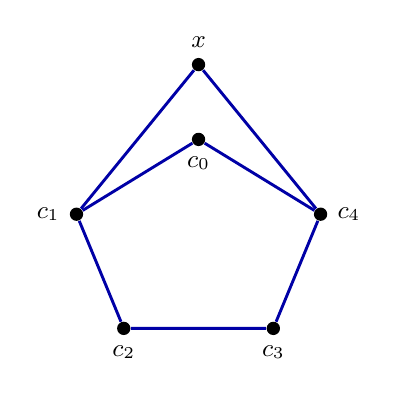
\begin{tikzpicture}[every node/.style={font=\small}]
  \node[graph vertex,label=below:$c_0$] (c0) at (0,1.4) {};
  \node[graph vertex,label=left:$c_1$] (c1) at (-1.55,0.45) {};
  \node[graph vertex,label=below:$c_2$] (c2) at (-0.95,-1) {};
  \node[graph vertex,label=below:$c_3$] (c3) at (0.95,-1) {};
  \node[graph vertex,label=right:$c_4$] (c4) at (1.55,0.45) {};
  \node[graph vertex,label=above:$x$] (x) at (0,2.35) {};
  \draw[marked edge] (c0)--(c1)--(c2)--(c3)--(c4)--(c0);
  \draw[marked edge] (c1)--(x)--(c4);
\end{tikzpicture}
\caption{A vertex $x$ in $U_0$ and its two marked edges to the cycle.}
\label{fig:odd-cycle-parts}
\end{figure}

To express $R$ in terms of the counts, let $L_R$ be the following
linear form in the six-position coordinates. The restriction to the
first five positions is the marked induced cycle. The coefficient
of a labeled extension is the number of neighbors of the sixth
position on the cycle if that position either has an unmarked edge
to the cycle or is adjacent to two consecutive cycle positions.
All other extensions have coefficient zero. A vertex outside $B$
with a cycle neighbor satisfies at least one of these two tests.
Indeed, if it fails both, it has at most two cycle neighbors and
all edges to them are marked. With only one such neighbor $c_i$,
its marked edge to $c_i$ has no endpoint in common with the
opposite cycle edge $c_{i+2}c_{i+3}$ and no edge joins their endpoints.
With two nonconsecutive marked neighbors, it belongs to one of
the sets $U_i$. Conversely, vertices of $B$ fail both tests.

Thus the sum over the sixth position is $R$ for each ordered
cycle. The denominators in \eqref{eq:q-definition} for five and
six positions differ by a factor of $D$. If $q_C>0$, this gives
$L_R=\frac{q_C}{D}\mathbb E[R]$, where the expectation is over a
uniformly chosen color-preserving map of the cycle pattern. If $q_C=0$,
there is no such map and $L_R=0$.

The five-cycle certificates give
\begin{equation}\label{eq:odd-moment-bounds}
 \frac{\mu}{D^2}\geq\gamma_C\Bigl(\frac{1}{8}-q_C\Bigr)-\epsilon_C,
 \qquad
 \frac{\mu}{D^2}\geq\gamma_R L_R-\epsilon_R.
\end{equation}
Both errors $\epsilon_C$ and $\epsilon_R$ are nonnegative. For the
first inequality we use either
$\gamma_C\geq\frac{99999}{100000}$ and $\epsilon_C\leq2\cdot10^{-9}$,
or $\gamma_C\geq\frac{6449}{10000}$ and $\epsilon_C\leq10^{-9}$.
For the second we use $\gamma_R\geq\frac{56425}{100000}$ and
$\epsilon_R\leq10^{-9}$. The files and checks are specified in
\textbf{Appendices~\ref{app:reproduction} and~\ref{app:cycle-estimates}}.

Suppose that $\mu\leq\mu_*$, $\gamma_C\geq g_C>0$ and
$\gamma_R\geq g_R>0$. Put
$q_*=\frac{1}{8}-\frac{\mu_*+\epsilon_C D^2}{g_C D^2}$.
The first inequality in \eqref{eq:odd-moment-bounds} gives
$q_C\geq q_*$ when $q_C<\frac{1}{8}$, and the bound holds directly
when $q_C\geq\frac{1}{8}$ because $q_*\leq\frac{1}{8}$. If $q_*>0$,
using the second inequality and $L_R=\frac{q_C}{D}\mathbb E[R]$
gives a cycle with $R\leq\mathbb E[R]$ and hence
\begin{equation}\label{eq:odd-choose-anchor}
 R\leq\frac{\mu_*+\epsilon_R D^2}{g_R Dq_*}.
\end{equation}
Verified upper bounds on either error can be used in this estimate.

\begin{lemma}\label{lem:simple-cycle-counts}
For the sets defined in \eqref{eq:odd-core-defs}, every vertex of
$U_i$ is adjacent to every vertex of $U_{i+1}$. Moreover,
$|B|=\frac{5D-R}{2}$ and $a_i=\frac{D-R}{2}+s_{i-2}+s_{i+2}$ for every $i$.
\end{lemma}

\begin{proof}
For every $x\in U_i$ and $y\in U_{i+1}$ we have $xy\in E(G)$. The
marked edges $xc_{i-1}$ and $yc_{i+2}$ are disjoint. The
definitions of the parts exclude $xc_{i+2}$ and $yc_{i-1}$, and
$c_{i-1}c_{i+2}$ is excluded because the cycle is induced. Since
the marked edges form a clique in $L(G)^2$, we must have
$xy\in E(G)$. Thus a vertex of $U_i$ has at most $s_i$ neighbors
outside $U_{i-1}\cup U_{i+1}$.

The sum $A=\sum_i a_i s_i$ bounds the number of incidences at vertices
of $B$ after excluding the edges between $U_i$ and $U_{i+1}$ for all
$i$. Each remaining edge with both ends in $B$ contributes two
incidences. Put $e_0=\sum_i a_i a_{i+1}$, the number of edges between
parts $U_i$ and $U_{i+1}$.
Solving \eqref{eq:odd-core-defs} gives
\begin{equation}\label{eq:odd-core-sums}
 a_i=t-\frac{R}{2}+s_{i-2}+s_{i+2},\qquad
 |B|=\frac{5D-R}{2}.
\end{equation}
Summing the five equations for $s_i$ gives the formula for $|B|$.
For $a_i$, the two disjoint pairs of indices
$\{i-2,i+1\}$ and $\{i-1,i+2\}$ are the neighbor pairs of
$i+2$ and $i-2$, respectively. Subtracting their sizes from $|B|$
gives $a_i=|B|-2D+s_{i-2}+s_{i+2}$.
\end{proof}

By substituting \eqref{eq:odd-core-sums} into $\sum_i a_i s_i$
and using $2e_0=\sum_i a_i(D-s_i)$, we obtain
\begin{equation}\label{eq:odd-core-capacity}
 A=tR-\frac{R^2}{2}+2\sum_i s_i s_{i+2},
 \qquad
 e_0=5t^2-\frac{Rt+A}{2}.
\end{equation}
When $D$ is odd, $R=5D-2|B|$ is odd as well. To bound $\sum_i s_i s_{i+2}$,
consider the cycle on the indices with edges $i,i+2$. If two
nonadjacent vertices have positive weights, move their combined
weight onto the vertex with the higher sum of neighboring weights.
With the other weights fixed, the sum of products does not decrease.
Repeating leaves positive weights on a clique of size at most two.
The sum of products is then at most $\frac{R^2}{4}$. When $D$ is odd, integrality reduces this bound to $\frac{R^2-1}{4}$, so
\eqref{eq:odd-core-capacity} gives $A\leq tR-\frac{1}{2}$.

\begin{lemma}\label{lem:odd-unit-slack}
If an induced five-cycle with five marked edges has $R=1$, then $D$ is odd and $m\leq f(D)$.
\end{lemma}

\begin{proof}
Let $i$ be the unique index with $s_i=1$. Every vertex of the other
four parts has degree $D$ from the consecutive pairs alone. Thus a
marked edge outside the consecutive pairs has both ends in
$U_i\cup(V(G)\setminus B)$. The marked edge $c_{i+2}c_{i+3}$ has both
ends in parts whose consecutive neighbors are outside $U_i$. Both
vertices already have degree $D$ from those pairs, so neither is
an endpoint of, or adjacent to an endpoint of, the proposed marked
edge. This contradicts the clique property. Hence $m\leq e_0$.
For $R=1$, \eqref{eq:odd-core-capacity} gives
$A=t-\frac{1}{2}$ and $e_0=5t^2-t+\frac{1}{4}=f(D)$.
\end{proof}

\subsection{The Bound \texorpdfstring{$\frac{5}{4}\Delta^2$}{5 Delta squared / 4} in Multigraphs}
\label{sec:multigraph}\label{sec:weighted-counts}

The simple support of a multigraph records every adjacency that can
join two marked edges. To count the marked edges themselves, we must
also record how many copies have each pair of endpoints.

Let $D\geq1$ be an integer. Take a loopless multigraph $G$ with
$\Delta(G)\leq D$ and fix a
nonempty strong clique of size $m$ in $G$. Mark the edges of the clique
and restrict the host to the subgraph induced by their endpoints.
Every edge joining two disjoint marked edges has both endpoints in this
subgraph. Keep all marked edges. Between each pair of adjacent vertices joined
only by unmarked edges, keep one of those edges. The simple support $G_{\rm s}$ of the reduced
host therefore retains all adjacencies needed for the marked edges to
form a strong clique. Color an edge of $G_{\rm s}$ red if its endpoints are joined by a
marked edge of $G$, and blue otherwise. Let $s$ be the number of red
edges. For each red edge $uv$, choose one marked edge with endpoints
$u,v$ as its \emph{base copy}. Call the remaining marked edges with
these endpoints \emph{extra copies}. The red edges form a strong
clique in $G_{\rm s}$.

Put
\[
 b=m-s,\qquad M=\frac{m}{D^2},\qquad S=\frac{s}{D^2},
 \qquad e=\frac{b}{m}.
\]
Here $M$ and $S$ are normalized clique sizes and $e$ is the fraction
of marked edges that are extra copies. Thus $S=M(1-e)$. For each edge $uv$ of $G_{\rm s}$ let $b_{uv}$ be its
number of extra copies, with $b_{uv}=0$ for blue edges. Write
$d_{\rm s}(v)=d_{G_{\rm s}}(v)$ and
$j_v=\sum_{u\in N_{G_{\rm s}}(v)}b_{uv}$.
Then $\sum_v j_v=2b$ and $d_{\rm s}(v)+j_v\le D$.

We now write $G$ for this reduced multigraph. To obtain a
$D$-regular multigraph, apply \textbf{Lemma~\ref{lem:regularization}} and give each new edge
color blue. The reduced host is induced in the completion, and all
new edges have multiplicity one. Thus the red edges, their
multiplicities and the adjacencies among their endpoints are
unchanged. In the next counts we use the simple support of the
completed multigraph.

Use colors $0,1,2$ for a pair with equal or nonadjacent images,
a blue edge and a red edge, respectively. Let $P$ be a connected colored pattern on $n$ positions
with at least one red edge. As in \textbf{Definition~\ref{def:patterns}},
any two red edges in $P$ either meet or have endpoints joined by a red
or blue edge. In the weighted counts, $P$ has no designated root edge.
Let $T$ be a set of red edges of $P$ that form a forest on the positions.
Define
\[
 Q(P,T)=\frac{1}{2mD^{n-2}}
       \sum_{\phi}\ \prod_{uv\in T} b_{\phi(u)\phi(v)},
 \qquad
 X(P,T)=\frac{Q(P,T)}{|\operatorname{Aut}(P,T)|}.
\]
Here $\phi$ runs over color-preserving maps of the positions of $P$
to the simple support, and $\operatorname{Aut}(P,T)$ is the group of
permutations of the positions that preserve the pair colors and the
edge set $T$. As before, color $0$ permits equal images. Each edge
of $T$ contributes its extra multiplicity, even if two edges of $T$
have the same image, as in \textbf{Figure~\ref{fig:weighted-maps}}.
The forest condition is imposed on the positions. We use patterns
with $2\le n\le6$ and $|T|\le3$. Write $X$ for the vector of coordinates
$X(P,T)$, using one representative for each isomorphism class of pairs
$(P,T)$.

\begin{figure}[htbp]
\centering
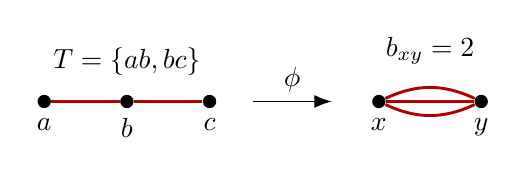
\begin{tikzpicture}[marked edge/.append style={draw=red!70!black}]
  \node[graph vertex,label=below:$a$] (a) at (0,0) {};
  \node[graph vertex,label=below:$b$] (b) at (1.05,0) {};
  \node[graph vertex,label=below:$c$] (c) at (2.1,0) {};
  \draw[marked edge] (a)--(b)--(c);
  \node[above=6pt] at (b) {$T=\{ab,bc\}$};
  \draw[-{Latex[length=2.2mm]}] (2.65,0)--node[above]{$\phi$}(3.65,0);
  \node[graph vertex,label=below:$x$] (x) at (4.25,0) {};
  \node[graph vertex,label=below:$y$] (y) at (5.55,0) {};
  \draw[marked edge] (x)--(y);
  \draw[marked edge] (x) to[bend left=25] (y);
  \draw[marked edge] (x) to[bend right=25] (y);
  \node[above=10pt] at (4.9,0) {$b_{xy}=2$};
\end{tikzpicture}
\caption{A weighted map with $\phi(a)=\phi(c)=x$ and $\phi(b)=y$.
Its weight is $b_{xy}^2=4$.}
\label{fig:weighted-maps}
\end{figure}

For the pattern $P$ consisting of a single red edge, summing over the
$2s$ oriented red edges of the simple support gives $Q(P,\varnothing)=1-e$. Summing their extra
multiplicities gives $Q(P,E(P))=e$, where $E(P)$ consists of the
single red pair. Each degree identity extends a fixed pattern
at a specified position. For a red extension, the unweighted and
weighted counts represent one base edge and the extra copies,
respectively. An extension to a blue neighbor counts its unique copy.
Together the blue and red extensions account for exactly
$D$ edge copies at the image of that position. The equations use
those extensions whose terms all occur in the model.

Choose two ordered marked edges independently, allowing the same
copy in both choices. Classify each choice as a base or an extra
copy. There are $(2s)^2$ ordered pairs of base copies,
$2(2s)(2b)$ ordered pairs with one base and one extra copy, and
$(2b)^2$ ordered pairs of extra copies. Each choice of the two
ordered copies determines the images of four positions in the
support. Their colors give a connected pattern because the two
edges belong to the strong clique. The forest weights count the
choices of an extra copy for each specified pair. As in
\eqref{eq:objective-vector}, divide the counts by $2mD^2$ and take
one half. The three contributions to the objective are
\[
 O_0=\frac{s^2}{mD^2},\qquad
 O_1=\frac{2sb}{mD^2},\qquad
 O_2=\frac{b^2}{mD^2}.
\]
Their sum is $M$ since $m=s+b$. More generally, adding an independent
ordered marked copy to a fixed pattern gives $2M Q(P,T)$
after normalization. Indeed, choosing the ordered copy multiplies the raw count by
$2m$, and the two new positions contribute a factor $D^2$ in the denominator. Replacing that copy by a base
or extra copy gives $2S Q(P,T)$ or $2Me Q(P,T)$. These formulas
give linear bounds when $M$, $S$ and $e$ are restricted to intervals.
For example, the bounds $e_-\le e\le e_+$ imply
\[
 O_2\le(e_-+e_+)\left(O_2+\frac{O_1}{2}\right)-e_-e_+M
\]
by expanding $M(e-e_-)(e_+-e)\ge0$.

Fix a type on $k$ positions and flags extending the type. In addition
to the colors, the type and flags specify forest edges as in $(P,T)$.
For a type map $\phi$, let $w(\phi)$ be the product of the extra
multiplicities on its specified forest edges. For the $i$th flag, on
$n_i$ positions, sum over the extensions of $\phi$ to that flag. Each
extension contributes the product of the extra multiplicities on its
specified forest edges outside the type. Let $v_i(\phi)$ be this sum
divided by $D^{n_i-k}$ and let $v(\phi)$ be the column vector with
entries $v_i(\phi)$. Then
\[
 \frac{1}{2mD^{k-2}}\sum_\phi w(\phi)v(\phi)v(\phi)^{\mathsf T}\succeq0.
\]
The matrix is a sum of outer products with nonnegative coefficients
because every extra multiplicity is a nonnegative integer. Its $(i,j)$ entry is a sum over pairs of extensions that agree on the type,
with denominator $2mD^{n_i+n_j-k-2}$. The two extensions may use the
same vertex outside the type. Group the pairs by the colors on the
remaining position pairs. Each resulting pattern uses the forest
edges in the type once, through $w(\phi)$. This writes each matrix
entry as a linear combination of coordinates $X(P,T)$. We use flag
lists for which these products lie in the specified pattern collection.
The same counting identity applies to the matrices formed from local
degrees and from counts of extensions satisfying degree constraints.

To bound $M$ we also need to count the edges at the vertices of an
induced red five-cycle in the reduced multigraph. Use the parts $U_i$
and remaining degrees $s_i$ from \eqref{eq:odd-core-defs} for the red
edges of its simple support. Call the vertices $c_0,\ldots,c_4$ of
the cycle its anchors, with indices modulo five, and put
$B=\bigcup_i U_i$. We call $B$ the core of this cycle.
Let $L$ be the number of blue pairs between $U_i$ and $U_{i+1}$,
summed over $i$. By \textbf{Lemma~\ref{lem:simple-cycle-counts}},
all pairs between these two parts are adjacent. Reserving one copy
for each such pair leaves at most $s_i$ incidences at each vertex of
$U_i$. Set $a_*=\frac{D-R}{2}$. Equations \eqref{eq:odd-core-sums}
and \eqref{eq:odd-core-capacity} applied to the simple support give
\begin{equation}\label{eq:multi-core-identities}
 a_i=a_*+s_{i-2}+s_{i+2},\qquad
 A=\sum_i a_is_i=\frac{RD}{2}-\frac{R^2}{2}
             +2\sum_i s_i s_{i+2}\le\frac{RD}{2}.
\end{equation}
In particular $R=5D-2|B|$ has the same parity as $D$.

We now bound the contribution of edges incident with vertices outside $B$.
Set $r=\frac{R}{D}$, $j=\frac{\sum_{i=0}^4j_{c_i}}{D}$,
$g=\frac{m}{D^2}-\frac{5}{4}$, and $\lambda=\frac{L}{D^2}$.

\begin{lemma}\label{lem:multigraph-cycle-counts}
If $g>0$, then $r>\frac{1}{2}$. For $\frac{1}{2}\le r\le1$,
\begin{equation}\label{eq:multi-joint}
 2g+2\lambda\le
 \frac{1+r}{2+r}\,r\left(r-\frac{1}{2}\right)
 -\frac{1+r^2}{2+r}\,j.
\end{equation}
\end{lemma}
\begin{proof}
The signature of a vertex $x$ is the set $\{i:xc_i\in E(G_{\rm s})\}$,
of size $k_x$. Summing the capacity $s_i$ at the five anchors gives
$K=\sum_{x\notin B}k_x\le R$. For $x\notin B$, let $h_x$ be its marked
degree, let $Q_x=|N_{G_{\rm s}}(x)\cap B|$, and let $b_x$ count its
blue pairs to $B$. For any marked edge $xy$, the union of the
signatures of $x$ and $y$ covers every edge of the cycle. In fact,
if $xy$ is disjoint from a cycle edge, the strong clique condition
gives an adjacency to one of the ends of that cycle edge. If $xy$
shares an endpoint with a cycle edge, its other cycle endpoint is
a neighbor of the shared vertex. Since a vertex cover of $C_5$ has
at least three vertices, a vertex with $k_x=0$ can have a marked
edge only to a vertex $y$ with $k_y\ge3$. In particular such an $x$
has no marked edge into $B$, since $k_y=2$ for $y\in B$.
A vertex outside $B$ of signature size two has at least one blue anchor pair. For
consecutive positions, a marked anchor pair would fail the strong
clique condition with the cycle edge opposite those positions. For
nonconsecutive positions, two marked anchor pairs would put the vertex
in $B$.

Every blue pair between consecutive classes uses two unmarked incidences
in $B$. The $b_x$ blue pairs of $x$ into $B$ use one unmarked incidence
in $B$ each, disjoint from the first set of incidences. The two
counts are illustrated in \textbf{Figure~\ref{fig:multigraph-cut}}.
Summing the marked incidences inside and outside $B$ gives
\begin{equation}\label{eq:multi-core-cut}
 2m\le D|B|-2L+\sum_{x\notin B}(h_x-b_x).
\end{equation}

\begin{figure}[htbp]
\centering
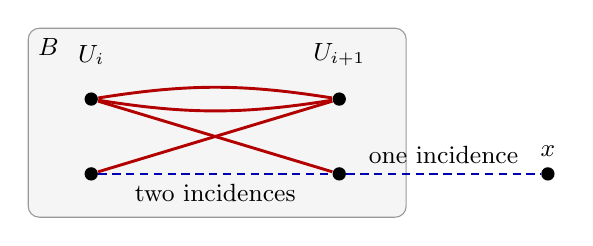
\begin{tikzpicture}[
  marked edge/.append style={draw=red!70!black},
  blue pair/.style={draw=blue!70!black,densely dashed,line width=0.95pt},
  font=\small
]
  \filldraw[fill=black!4,draw=black!40,rounded corners=4pt]
    (-0.65,-0.55) rectangle (4.15,1.85);
  \node[anchor=north west] at (-0.65,1.85) {$B$};
  \node at (0.15,1.51) {$U_i$};
  \node at (3.3,1.51) {$U_{i+1}$};
  \node[graph vertex] (a) at (0.15,0.95) {};
  \node[graph vertex] (b) at (0.15,0) {};
  \node[graph vertex] (c) at (3.3,0.95) {};
  \node[graph vertex] (d) at (3.3,0) {};
  \node[graph vertex,label=above:$x$] (x) at (5.95,0) {};
  \draw[marked edge] (a) to[bend left=9] (c);
  \draw[marked edge] (a) to[bend right=9] (c);
  \draw[marked edge] (a)--(d);
  \draw[marked edge] (b)--(c);
  \draw[blue pair] (b)--node[below] {two incidences} (d);
  \draw[blue pair] (d)--node[above] {one incidence} (x);
\end{tikzpicture}
\caption{A blue edge between consecutive parts contributes twice to
the degree sum on $B$. A blue edge from $x\notin B$ to $B$ contributes
once. Both copies of a marked pair contribute to marked degree.}
\label{fig:multigraph-cut}
\end{figure}

We first bound the total outside contribution after charging $b_x$ against
the core capacity. Suppose $k_x=1$ and $x$ has a marked edge to a vertex of $B$.
We show that $b_x\ge a_*+1$. Let $j$ be the sole index in the signature of $x$, and write $xy$ for
its marked edge with $y\in U_i$. Since $\{j,i-1,i+1\}$ covers the
cycle, $i=j\pm2$. Of the two cycle neighbors of $c_j$, let $c_k$
be the one nonadjacent to $y$. For each $u\in U_j$ the edge $c_ku$
is marked. Comparing it with $xy$ gives $xu$ or $yu$ in the support.
The edge $xy$ uses one of the $s_i$ extra incidences at $y$, so
$y$ has at most $s_i-1$ neighbors in $U_j$. At least
$a_j-s_i+1\ge a_*+1$ vertices of $U_j$ are therefore adjacent to
$x$. Each of these edges is blue, since $\{j,j-1,j+1\}$ does not
cover the cycle. If $xy$ is marked with $k_x=1$ and $k_y=2$, the union of their
signatures is a vertex cover of the cycle and hence has size three.
Whenever the union on an outside marked edge has size three, its two
omitted positions are nonconsecutive. Every red edge from either
omitted anchor into $B$ forces its other end to be adjacent to at least
one end of the outside marked edge. The core neighborhoods of those
ends therefore cover three classes. The other two classes have total
size at most $D$, so the three classes contain at least $|B|-D=D+a_*$
vertices. Each end uses one degree unit on the outside marked edge,
and so each sees at least $a_*+1$ vertices of $B$. If the end of
signature size one has no marked edge into $B$, these pairs are blue.

We redistribute the quantities $h_x-b_x$ over vertices outside $B$.
A vertex of signature size one with a marked core neighbor or a
marked neighbor of signature size two has $b_x\ge a_*+1$. Since
$h_x+b_x\le D$, it retains a contribution at most $R-2$. Any other
vertex of signature size one sends $\frac{1}{2}$ per marked copy to
its neighbors, all of which have signature size at least three. Its
remaining contribution is at most $\frac{D}{2}$. A vertex $x$ of
signature size zero with a marked neighbor of signature size three
has $b_x=Q_x\ge a_*$ by the comparison with the two omitted anchors.
It distributes its positive contribution uniformly over its marked
edges. Since $h_x\le D-Q_x$, the amount per copy is at most
$\frac{2R}{D+R}$. The other vertices of signature size zero use the
same rule, with at most one per copy and with recipients of
signature size at least four. We discard any negative contribution
left at a vertex of signature size zero.

A recipient of signature size three with a marked neighbor of
signature size zero also sees at least $a_*$ vertices of $B$, so it
has at most $\frac{D+R}{2}$ marked copies outside $B$. Multiplying
this bound by the larger of the two sending rates shows that it
receives at most $\max\{\frac{D+R}{4},R\}$. If it has no marked
neighbor of signature size zero, it receives at most $\frac{D}{2}$.
A recipient with at least four positions receives at most $D$.
Adding each recipient's own contribution, at most $D$, shows that
the total contribution at every outside vertex is at most
$k_x\max\{\frac{D}{2},R\}$ for $R\le D$. By \eqref{eq:multi-core-cut},
\begin{equation}\label{eq:multi-rough-discharge}
2m\le D|B|-2L+\max\left\{\frac{D}{2},R\right\}K.
\end{equation}

If $R\le \frac{D}{2}$, the right-hand side of \eqref{eq:multi-rough-discharge}
is at most $D|B|+\frac{D}{2}R=\frac{5}{2}D^2$.
Thus $g>0$ implies $r>\frac{1}{2}$.

Assume now that $\frac{1}{2}\le r\le1$. The $K$ adjacencies from the
five cycle vertices to the exterior and the $\sum_i j_{c_i}$ extra marked
incidences at those vertices use disjoint units of the remaining
degree $R$. Thus $K\le R-\sum_i j_{c_i}$.
Divide all vertex counts and degrees by $D$, and all
edge counts by $D^2$. Write $\eta=\frac{1-r}{2}$, $v=\frac{1+r}{2}$
and $\rho=\frac{2r}{1+r}$. An outside marked edge whose signatures
have union of size three has two ends each with normalized core
degree at least $\eta$. Each end has outside marked degree at most
$v$.

Let $x$ count the vertices of signature size one with a marked
neighbor in the core or a marked neighbor of signature size two.
Their total contribution in \eqref{eq:multi-core-cut}, in the
normalized units, is denoted by $C_1$. Each of these vertices has
at least $\eta$ blue pairs into the core, and $C_1\le rx$. Let
$p_2,p_3$ count the marked edges from these vertices to vertices of
signature size two and of signature size at least three, respectively.
Let $n_2$ count their neighbors of signature size two via a marked
edge. Also let $z_3,z_0$ count the vertices of signature size three
and of signature size zero, respectively, that meet a marked edge
joining these two groups. Denote the count of such edges by $p_{03}$.
The three groups counted by $n_2,z_3,z_0$ are disjoint. Each of their
vertices uses at least $\eta$ of the core capacity by the comparison
with the two omitted anchors, and $p_2\le v n_2$ and
$p_{03}\le v\min\{z_0,z_3\}$.

By \eqref{eq:multi-core-identities}, the total normalized capacity
of the core after reserving its consecutive pairs is at most
$\frac{r}{2}$. Deduct the core capacity used by the groups counted
by $x,n_2,z_3,z_0$. To bound $C_1$, add the exterior marked
counts $p_2+p_3$ and deduct the blue core pairs at the vertices
counted by $x$. This gives
$C_1\le\frac{r}{2}-2\eta x-\eta(n_2+z_3+z_0)+p_2+p_3$.
With $\theta=\frac{2r-1}{2+r}$ and $c=r-\theta=\frac{1+r^2}{2+r}$,
take weights $1-\theta,\theta$ on the two bounds for $C_1$ to get
\begin{equation}\label{eq:multi-joint-first}
 C_1\le cx+\frac{\theta r}{2}
     +\theta(p_2+p_3)-\theta\eta(n_2+z_3+z_0).
\end{equation}

For the other outside vertices, use the redistribution leading to
\eqref{eq:multi-rough-discharge}. A vertex of signature size two
retains at most one. Assign $\theta p_2-\theta\eta n_2$ in
\eqref{eq:multi-joint-first} to the group of such vertices. Since
$p_2\le v n_2$, its additional contribution is at most $\theta r$
per vertex, or at most $c=\frac{1}{2}+\frac{\theta r}{2}$ per signature
position after adding the original contribution.

For a vertex of signature size at least four, let $d_1$ be its
marked degree to the group counted by $x$. None of those edges
transfers any contribution to it, so its own and received
contributions sum to at most $2-d_1$. The corresponding bound for a
vertex of signature size three with no marked neighbor of signature
size zero is $\frac{3}{2}-\frac{d_1}{2}$. Adding the corresponding
$\theta d_1$ from $\theta p_3$ gives at most $c$ per signature
position in both cases, since $c\ge\frac{1}{2}$ and $\theta\le\frac{1}{3}$.

For the group counted by $z_3$, write $d_{1,3}$ for its marked
degree to the group counted by $x$. The vertices counted by $z_3$
have outside marked degree at most $v$ and receive at most
$\frac{1}{2}$ per marked copy, except for edges to the vertices
counted by $z_0$, which can transfer up to $\rho$ each. The total
after adding the corresponding terms of \eqref{eq:multi-joint-first}
is at most
\[
 \left(1+\frac{v}{2}\right)z_3
 -\left(\frac{1}{2}-\theta\right)d_{1,3}
 +\left(\rho-\frac{1}{2}\right)p_{03}-\theta\eta(z_3+z_0).
\]
Use $z_0\ge\frac{p_{03}}{v}$, then $p_{03}\le v z_3$, to
bound this by $(1+\rho v-2\theta\eta)z_3=3c z_3$. The second
substitution is valid because
$\rho-\frac{1}{2}-\frac{\theta\eta}{v}\ge0$ for $\frac{1}{2}\le r\le1$.
This accounts for all terms of \eqref{eq:multi-joint-first}.
The vertices of signature size one outside the group counted by
$x$ retain at most $\frac{1}{2}$ each. Thus the right side of
\eqref{eq:multi-core-cut}, divided by $D^2$, is at most
$\frac{5-r}{2}-2\lambda+c(r-j)+\frac{\theta r}{2}$.
Subtracting $\frac{5}{2}$ proves \eqref{eq:multi-joint}.

\end{proof}

Apply the simple-graph five-cycle counts to the red edges of
$G_{\rm s}$. Completing the simple support to a $D$-regular simple
graph adds only blue edges. All vertices of a red five-cycle and of
its five parts are incident with red edges. They therefore belong
to the old graph, which is induced in the completion. Thus the
completion preserves both the red five-cycles and their five
parts. Write $q_C$ for the number of ordered induced red five-cycles
divided by $2sD^3$ and $L_R$ for the sum of $\frac RD$ over these
cycles divided by the same quantity. If each such cycle satisfies
$R\geq\alpha D$, then summing this inequality gives $L_R\geq\alpha q_C$.

Applying the simple-graph certificate inequality to four choices
of objective gives
\begin{equation}\label{eq:support-projection-four}
\begin{aligned}
 S-0.99999q_C
   &\le \frac{5}{4}-\frac{0.99999}{8}+2\cdot10^{-9},\\
 S+0.5682L_R
   &\le \frac{5}{4}+10^{-9},\\
 S+0.4897(L_R-0.32q_C)
   &\le \frac{5}{4}-\frac{0.4897\cdot0.32}{8}+2\cdot10^{-9},\\
 S+0.45119\left(L_R-\frac{q_C}{2}\right)
   &\le \frac{5}{4}-\frac{0.45119}{16}+2\cdot10^{-9}.
\end{aligned}
\end{equation}
The coefficients and the error allowances in
\eqref{eq:support-projection-four} are rational.
\textbf{Appendix~\ref{app:multi-projection}} specifies the
four certificate checks. To see why the displayed coefficients
suffice, write each certified inequality as $S+\gamma Y\leq
\frac54+\varepsilon$, moving the multiple of $\frac18$ to the left.
For $Y\geq0$, replacing $\gamma$ by a smaller nonnegative coefficient
preserves the inequality. For $Y<0$ the bound follows from
$S\leq\frac54$.

For a given $\alpha>0$, substitute $L_R\geq\alpha q_C$ in
\eqref{eq:support-projection-four}. Each of the four inequalities
now has the form $S\leq a_i-b_iq_C$. Include $S\leq\frac54$ as
a fifth inequality, with $a_5=\frac54$ and $b_5=0$. Thus
\[
 S\leq S_{\max}(\alpha):=
 \max_{x\geq0}\min_{1\leq i\leq5}(a_i-b_ix),
 \qquad e\geq1-\frac{S_{\max}(\alpha)}{M}.
\]
The second line of \eqref{eq:support-projection-four} has
$b_2=0.5682\alpha>0$. The minimum of the five lines is continuous
and piecewise linear and tends to $-\infty$ as $x$ tends to infinity.
Its maximum is therefore attained at zero or at the nonnegative
intersection of two lines with different slopes. This gives a finite
rational calculation for $S_{\max}(\alpha)$.

These inequalities can also be imposed directly on $X$. Multiplying
each simple-graph inequality by $1-e=\frac{s}{m}$ changes the cycle
normalization from $2sD^3$ to $2mD^3$. Its term $(1-e)S$ is $O_0$,
and the same factor changes $L_R$ to the corresponding weighted
coordinate sum. All terms of the resulting inequality are linear
in the weighted counts.

Let $k\geq3$ and let $K$ be the vertex set of a red $K_k$ in the weighted host.
For each vertex $v$ put $a_v=|N_{G_{\rm s}}(v)\cap K|$ and let
$h_v$ and $d_{\rm blue}(v)$ count the marked and the unmarked edges
incident with $v$, respectively. Let $m_K$ count the marked edges with
both endpoints in $K$, with multiplicity, and put
$J_K=\sum_{v\in K}j_v$. For a marked edge $uv$, the set
$(N_{G_{\rm s}}(u)\cup N_{G_{\rm s}}(v))\cap K$ meets every edge
of the red clique. Indeed, a disjoint red edge in $K$ must have an
endpoint adjacent to $u$ or $v$, and the same holds when the red
edge shares an endpoint with $uv$. Every vertex cover of $K_k$ has
size at least $k-1$, so $a_u+a_v\geq k-1$. If $u\in K$, then
$a_u=k-1$ and $a_v\geq1$. If both endpoints lie in $K$, then
$a_u+a_v=2(k-1)$. Summing over all marked edges with multiplicity gives
\[
 (k-1)m+\sum_{v\in K}h_v+(k-3)m_K
 \le\sum_v a_vh_v
 \le D(kD-J_K)-\sum_{v\in K}d_{\rm blue}(v).
\]
For the upper bound, $\sum_v a_v=\sum_{v\in K}(D-j_v)=kD-J_K$
in the regular completion. Moreover, $a_vd_{\rm blue}(v)$ is at
least the number of blue neighbors of $v$ in $K$. Summing this
last inequality counts each blue incidence at $K$ and gives the
upper bound on $\sum_v a_vh_v$, since $h_v=D-d_{\rm blue}(v)$.
Using $\sum_{v\in K}(h_v+d_{\rm blue}(v))=kD$ now gives
\[
 (k-1)m\le kD(D-1)-DJ_K-(k-3)m_K.
\]
For $k=5$, the right side is at most $5D(D-1)-20$. Thus $4m\leq5D(D-1)-20$ if a red $K_5$ exists.
This is impossible when $m\geq\frac54D^2$. For odd $D$ it is also
impossible when $m=f(D)+1$, since then $4m=5D^2-2D+5$.
The coordinates of every pattern containing a red $K_5$ are
therefore zero in either case.

Fix a red edge $xy$. Let $U=N_{G_{\rm s}}(x)\setminus (N_{G_{\rm s}}(y)\cup\{y\})$
and let $W$ be the vertices adjacent to neither $x$ nor $y$. In the
host induced on $U\cup W$, mark only the previously marked edges
between $U$ and $W$. Edges within a part can still join endpoints of
these marked edges. For each marked edge $uv$ between $U$ and $W$, and
each red neighbor $z$ of $y$, the strong clique condition for $uv$
and $yz$ forces $uz$ or $vz$ to be a host edge. All such vertices $z$ lie
outside $U\cup W$, and different $z$ give different edges incident
with $u$ or $v$ that are absent from the induced host. Hence the Ore-degree $\sigma$ of the bipartite
marked subgraph in this induced host is at most $2D$ minus the
number of red neighbors of $y$.

If there is a marked edge between $U$ and $W$, the corresponding
upper bounds are
\[
 \frac{2973}{10000}\sigma^2\quad\text{for all copies},\qquad
 \frac{273323}{10^6}\sigma^2\quad\text{for base copies},\qquad
 \frac14\sigma^2\quad\text{for extra copies}.
\]
We give the counts that yield these bounds. In the induced host
let $H$ be the bipartite graph of marked edges between $U$ and $W$,
with their multiplicities. Suppose $H$ is nonempty, put $h=\Delta(H)$, and take
a vertex $v$ of marked degree $h$. Let $A=N_H(v)$,
$B'=V\setminus N[v]$ (where $V$ and $N[v]$ refer to the induced
host), $p=|A|$ and $\ell=\sigma-d(v)$, with $d(v)$ the degree in
the host. Every $a\in A$ has host degree at most $\ell$ since $va$
is marked. Let $T$ be the number of marked edges meeting $A$,
$P$ the number of unmarked edges from $A$ to $B'$, and
$F=H[B']$. Write $f=|E(F)|$ and $u=\Delta(F)$, with $u=0$ if
$F$ is edgeless. Every marked edge omitted by the counts $T$ and
$f$ has an endpoint in $N(v)\setminus A$. This set has at most
$d(v)-h$ vertices. Consequently
\[
 |E(H)|\leq h(\sigma-h)-h\ell+T+f,\qquad T+P\leq p\ell .
\]
For each $a\in A$, its neighbors in $B'$ meet every edge of $F$.
Since neither endpoint of that edge is adjacent to $v$, one must
be adjacent to $a$ to join the edge to $va$. Thus $f\leq u\ell$.
The same observation shows that the Ore-degree of the marked edges
in the host induced on $B'$ is at most $\sigma-p$. Indeed, for
each of the $p$ vertices of $A$, at least one edge to an endpoint
of the marked edge is lost when the host is restricted to $B'$.

First count all marked copies. On each pair joined by a marked
edge, remove the unmarked copies. On every other adjacent pair
retain one unmarked edge. This preserves all marked edges and all
adjacencies, and $\sigma$ still bounds the degree sum on each marked
edge. Use the counts above for this reduced host. Let $X'$ comprise the vertices of
$B'$ in the same part of $H$ as $v$. For $x\in X'$, let $h_x$
count the marked edges from $x$ to $A$, with multiplicity, and put
$f_x=d_F(x)$.
Each marked edge of $F$ has one endpoint in $X'$. For every
$a\in A$ it has an endpoint adjacent to $a$. The adjacency to $a$
either has an unmarked copy or is marked and meets the endpoint
in $X'$. Counting these possibilities yields
\[
 pf\leq uP+\sum_{x\in X'} h_xf_x .
\]
If $T,f>0$, let $\alpha=\frac{T}{T+f}$ and $\gamma=\frac{f}{T+f}$.
The identity
$(h_x+f_x)(\gamma^2h_x+\alpha^2 f_x)-h_x f_x
=(\gamma h_x-\alpha f_x)^2$ and the bound $h_x+f_x\leq h$
give $\sum_{x\in X'} h_xf_x\leq h(\gamma^2T+\alpha^2 f)
=\frac{hTf}{T+f}$. Substituting the resulting lower bound for
$P$ in $T+P\leq p\ell$ gives
\[
 |E(H)|\leq h(\sigma-h)+\left(1-\frac hp\right)T
       +\left(1-\frac hu\right)f
       +\frac{h^2Tf}{pu(T+f)} .
\]
If $f=0$, the previous counts give $|E(H)|\leq h(\sigma-h)$.
The induced host on $B'$ has fewer marked edges, since it omits
all marked edges at $v$. Applying bounds for this smaller graph with
Ore-degree at most $\sigma-p$ gives upper bounds for $f$.
The proof notes in the repository~\cite{FGSTCode} give further necessary
inequalities by comparing the marked neighborhoods in $A$ of
two vertices of $X'$. For example, if $x,x'\in X'$ are nonadjacent,
every vertex of $N_H(x)\cap A$ that is not adjacent to $x'$ must
be adjacent to every vertex of $N_H(x')\cap A$ that is not adjacent
to $x$. Otherwise two marked edges would have no edge joining their
endpoints. The rational interval check in \textbf{Appendix~\ref{app:ore-replay}}
uses these neighborhood inequalities and the bounds for the smaller
graph. It excludes $|E(H)|>\frac{2973}{10000}\sigma^2$ over the full
range of $\frac{h}{\sigma},\frac ph,\frac uh,\frac{T}{\sigma^2}$
and $\frac{f}{\sigma^2}$.

For the base copies, pass to the simple support, mark one edge on
each marked pair, and take the host induced on their endpoints.
This preserves every adjacency that joins two disjoint marked edges.
Let $s'$ be the number of marked edges in this simple host and let
$\sigma'\leq\sigma$ be their Ore-degree. Every vertex has a marked
neighbor, so its degree is at most $\sigma'-1$. For a connected
pattern $P$ on $k$ positions rooted at an ordered marked edge,
normalize its map count by $2s'(\sigma')^{k-2}$. The resulting
coordinate $q_P$ lies in $[0,1]$ by the spanning-tree bound and
vanishes if the marked edges of $P$ contain an odd cycle.
The count of two ordered marked edges in \eqref{eq:objective-value}
now gives the objective $\frac{s'}{(\sigma')^2}$.
The extension sum at one position is at most $q_P$. If $ij$ is a
marked edge of $P$, the two extension sums at $i$ and $j$ together
are at most $q_P$, since the sum of the two image degrees is at
most $\sigma'$. The moment matrices remain positive semidefinite
by \textbf{Lemma~\ref{lem:moment}}. The rational certificate in
\textbf{Appendix~\ref{app:ore-replay}} combines the extension inequalities
with nonnegative multipliers and the moment matrices with
positive semidefinite matrices. Each negative residual coefficient
is charged its absolute value, using $0\leq q_P\leq1$. The resulting
upper bound on $\frac{s'}{(\sigma')^2}$ is
$\frac{27332270490572378277}{10^{20}}<\frac{273323}{10^6}$.
This proves the asserted bound for base copies.

Finally, mark only the extra copies between $U$ and $W$, reserving
one base copy on each originally marked pair as an unmarked edge.
Every adjacent pair of vertices now has an unmarked edge joining it.
Apply the same counts with $H$ the graph of these extra copies.
The result is immediate if $H$ is empty. Otherwise, for
every pair consisting of $a\in A$ and an edge of $F$, the
joining adjacency has an unmarked copy, and each such copy serves
at most $u$ edges of $F$. Therefore $pf\leq uP$.
If $f=0$, the first two inequalities give $|E(H)|\leq
h(\sigma-h)$ because $p\leq h$. If $f>0$, then $u>0$, and
\[
 |E(H)|\leq h(\sigma-h)-(h-p)\ell+
          \left(1-\frac pu\right)f
 \leq h(\sigma-h)+\left(1-\frac hu\right)f
 \leq h(\sigma-h).
\]
Here the second inequality uses $f\leq u\ell$ and $p\leq h$,
and the last uses $u\leq h$. Finally $h(\sigma-h)\leq
\frac{\sigma^2}{4}$.

Multiplying any of the three bounds by the nonnegative forest
weight of the root and summing over root maps gives a linear
inequality for $X$. Expanding a neighbor count uses one further
position, and expanding its square or counting another edge uses
two.

Write $AX=(1,0,\ldots,0)^{\mathsf T}$ for the degree and sampling
equations, $NX\le0$ for the linear inequalities, and $G_i(X)\succeq0$
for the matrix inequalities. To bound $M$, take a vector
$\lambda$ with first entry $\lambda_0$, a nonnegative vector $\rho$, and matrices $P_i$
given as nonnegative sums of rational rank-one outer products.
Let $G_i^*$ be the adjoint defined by
$(G_i^*(P_i))^{\mathsf T}X=\tr(P_iG_i(X))$. The constraints give $\rho^{\mathsf T}NX\leq0$ and
$\tr(P_iG_i(X))\geq0$. Thus, for every feasible $X$,
\[
 \left(A^{\mathsf T}\lambda+N^{\mathsf T}\rho
        -\sum_iG_i^*(P_i)\right)^{\mathsf T}X
 \le\lambda_0 .
\]
Let $r$ be the coefficient vector on the left minus the coefficient
vector of $M$. If $0\le X_j\le U_j$ for each coordinate $j$, then
$M\le\lambda_0+\sum_{j:r_j<0}(-r_j)U_j$. For a coordinate $X(P,T)$,
an upper bound is
$\frac{1-e}{|\operatorname{Aut}(P,T)|}$ for $T=\varnothing$ and
$\frac{e}{|\operatorname{Aut}(P,T)|}$ otherwise. To obtain it, start at
a red edge, in $T$ if $T$ is nonempty, and extend along a
spanning tree containing $T$. Each new position contributes at
most $D$ in support count or extra multiplicity. The certificates
also use bounds on sums of coordinates of equal order and
equal forest size, obtained by counting all labeled spanning
trees containing the specified red root. Positive residuals
can be dropped since the coordinates are nonnegative. With these bounds the total correction is affine in $e$, so
its maximum over the allowed interval is attained at an endpoint. For an infeasibility certificate, the objective
is zero and the compensated right side is negative.

\begin{lemma}\label{prop:multi-uniform}
Every strong clique of size $m$ in a finite loopless multigraph of maximum
degree at most $D$ satisfies $m\le\frac{5D^2}{4}$. If $m>0$, $D>0$, and
$M\ge\frac{4967}{4000}$,
then $e<\frac{1}{4}$.
\end{lemma}

\begin{proof}
If $m=0$ the asserted bound holds. Otherwise $D>0$, and the
red edges form a strong clique of size $s$ in the simple support,
which has maximum degree at most $D$. Thus
\textbf{Lemma~\ref{prop:quadratic-bound}} gives $S\leq\frac{5}{4}$.
The five-position certificates in \textbf{Appendix~\ref{app:weighted-final-checks}}
exclude $M\geq\frac{4967}{4000}$ and $e\geq\frac14$ simultaneously,
giving the second assertion. They also give
$e<\frac{421}{2000}$ for $M\geq\frac54$ and $M<1.28492$ for
$M>\frac54$.

Suppose that $M>\frac54$. For an induced red five-cycle put
$r=\frac RD$ and $g=M-\frac54$. The degree estimates in
\textbf{Lemma~\ref{lem:multigraph-cycle-counts}} give $r>\frac12$.
When $r\leq1$, \eqref{eq:multi-rough-discharge} implies
$2g\leq r(r-\frac12)$, and \eqref{eq:multi-joint} gives the
stronger inequality
\[
 2g\leq\frac{1+r}{2+r}r\left(r-\frac12\right).
\]
Both right-hand sides are increasing on $[\frac12,1]$.
For a proposed lower bound $M_-$ on $M$, substitute
$g\geq M_--\frac54$ and solve for a lower bound $\alpha$ on $r$.
For example, if $M_-=1.283$, then
$0.6084(0.6084-\frac12)<2(1.283-\frac54)$, so $r>0.6084$.
All values of $\alpha$ in \textbf{Table~\ref{tab:uniform-chain}}
are at most one and hence also apply when $r>1$.
It follows from \eqref{eq:support-projection-four} that
$e\geq1-\frac{S_{\max}(\alpha)}{M_-}$. This argument includes the
case of no induced red five-cycle, when $L_R=q_C=0$.

\begin{table}[htbp]
\centering
\caption{Intervals excluded by the six-position certificates. Each row
gives a certified upper bound for $M$ strictly below $M_-$.}
\label{tab:uniform-chain}
\begin{tabular}{@{}rrrr@{}}
\toprule
$M_-$ & $M_+$ & $\alpha$ & Lower bound on $e$\\
\midrule
1.283 & 1.28492 & 0.6084 & 0.051\\
1.279 & 1.283 & 0.6446 & 0.049\\
1.274 & 1.279 & 0.6242 & 0.0445\\
1.268 & 1.274 & 0.5978 & 0.0395\\
$\frac54$ & 1.274 & 0.5 & 0.0225\\
\bottomrule
\end{tabular}
\end{table}

For each row, assume $M_-\leq M\leq M_+$. On this interval the
weighted counts satisfy the lower bound on $e$ in the last column
and $e<\frac{421}{2000}$. The rational certificates for these
intervals, including the corrections for negative residuals, are
specified in \textbf{Appendix~\ref{app:weighted-final-checks}}. The first three
rows successively exclude $M\geq1.283$, $M\geq1.279$ and
$M\geq1.274$. The last row now applies throughout the remaining
interval and gives
\[
 M\leq\frac{124968062205915704703985647}
                 {100000000000000000000000000}<\frac54,
\]
contrary to $M>\frac54$.
\end{proof}

The quadratic bound gives $m\leq f(D)$ for even $D$. For odd $D$
we shall need one further estimate on the number of extra copies.

\begin{lemma}\label{lem:multi-extra}
Suppose $b>0$ and set $A=\frac{\sum_v j_v^2}{2bD}$. Then
\[
 M\le 2-\left(2+\frac{1}{D}\right)A-\frac{1}{D^2},
 \qquad
 Me\le 2A(1-A)-\frac{A}{D}.
\]
In particular, $e\le 1-\frac{M}{2}$ whenever $M\ge1$.
\end{lemma}

\begin{proof}
Count ordered pairs $(g_1,g_2)$ of marked edges, allowing $g_1=g_2$.
For each ordered pair of marked edges, the strong clique property gives adjacent vertices
$u,v$ with $u$ an endpoint of $g_1$ and $v$ an endpoint of $g_2$.
If the edges share an endpoint, there are at least two
such ordered pairs $(u,v)$. Among the $b^2$ ordered pairs of extra copies,
exactly $\sum_v j_v^2-\sum_{uv\in E(G_{\rm s})}b_{uv}^2$ share an
endpoint. The second sum removes the
double count of pairs sharing both endpoints. The result is at least
$\frac{1}{2}\sum_v j_v^2$, since $\sum_v j_v^2\ge2\sum_{uv}b_{uv}^2$.
Counting the ordered adjacent endpoints gives
\[
 b^2+\frac{1}{2}\sum_v j_v^2
 \le 2\sum_{uv\in E(G_{\rm s})}j_uj_v
 \le \sum_v j_v^2(D-j_v).
\]
The last inequality follows from $2j_uj_v\le j_u^2+j_v^2$ and
$d_{\rm s}(v)\le D-j_v$. The quantities $\frac{j_v}{D}$ have
weighted mean $A$ with weights $\frac{j_v}{2b}$. Expanding
$\sum_v \frac{j_v}{2b}\bigl(\frac{j_v}{D}-A\bigr)^2\geq0$
gives $\sum_v j_v^2(D-j_v)\le 2bD^2A(1-A)$.
This gives the upper bound on $Me=\frac{b}{D^2}$.

Let $h_v$ be the number of base copies incident to $v$. Among ordered pairs
with the extra copy first and the base copy second, at least
$b$ share an endpoint, since each extra copy shares its two
endpoints with its own base copy. Using $h_v\le D-j_v$ gives
\[
 sb+b\le \sum_v j_v\sum_{u\in N_{G_{\rm s}}(v)} h_u
 \le D\sum_v j_v d_{\rm s}(v)-2\sum_{uv\in E(G_{\rm s})}j_uj_v.
\]
Using $d_{\rm s}(v)\le D-j_v$ and the lower bound on
$2\sum_{uv\in E(G_{\rm s})}j_uj_v$ gives
\[
 b(m+1)\le 2bD^2-\left(D+\frac{1}{2}\right)\sum_v j_v^2.
\]
Divide by $bD^2$ to obtain the first inequality. For $M\ge1$ we
have $0\le A\le 1-\frac{M}{2}\le\frac{1}{2}$. The function $2x(1-x)$ is
increasing on $[0,\frac{1}{2}]$, so $Me\le M(1-\frac{M}{2})$.
\end{proof}

\begin{lemma}\label{lem:multi-even-equality}
Suppose the host has positive even maximum degree $D$ and the
number of marked copies is $\frac{5D^2}{4}$. The host induced by
the marked endpoints is a blow-up of $C_5$ with all five parts of
size $\frac{D}{2}$. Every edge of that blow-up is single and marked.
\end{lemma}

\begin{proof}
The five-position multiplicity bound applies at $M=\frac{5}{4}$ and
gives $e<0.2105$. If every induced red five-cycle had
$\frac{R}{D}\ge\frac{1}{2}$, the support bound in \eqref{eq:support-projection-four} would give $S\le1.22181$ and
hence $e>0.0225$. These bounds satisfy the hypotheses of the last six-position certificate in \textbf{Table~\ref{tab:uniform-chain}}, whose upper bound is strictly less than
$\frac{5}{4}$. Thus there is a cycle with $R<\frac{D}{2}$.

Apply the redistribution leading to \eqref{eq:multi-rough-discharge}
at this cycle. For every outside vertex $x$ with $k_x>0$, its
resulting contribution is strictly less than $\frac{k_xD}{2}$.
For $k_x=1$, a vertex either keeps at most $R-2$ or sends half of
its marked degree and has a blue anchor edge. For $k_x=2$, there
is a blue anchor edge and no incoming transfer. For $k_x=3$ with
a marked neighbor of signature size zero, the incoming transfer
is at most $\max\{\frac{D+R}{4},R\}<\frac{D}{2}$. Without such a
neighbor, it is at most $\frac{D-3}{2}$, since the three anchor
adjacencies use degree units inside the core. For $k_x\ge4$,
the transfer is at most $D-k_x$ and its own contribution is
at most $D$. Vertices of signature size zero retain no positive
contribution. Since $K\le R$, the presence of an outside vertex
of positive signature size would give $2m<D|B|+\frac{DK}{2}
\le\frac{5D^2}{2}$ by \eqref{eq:multi-core-cut}.

Hence $K=0$. Now $2m\le D|B|=\frac{D(5D-R)}{2}$, so $R=0$.
By \eqref{eq:multi-core-identities}, the five part sizes are
$\frac{D}{2}$. For a vertex of $U_i$, the neighbors in
$U_{i-1}\cup U_{i+1}$ already use all $D$ degree units. There are
$\frac{5D^2}{4}$ edges on these pairs. Any marked copy outside
$B$ would require an outside vertex of positive signature size.
Thus all edges in the blow-up are marked, and $B$ contains every
marked endpoint.
\end{proof}


We finish with a consequence used in \textbf{Section~\ref{sec:exact}}
to force an induced red five-cycle. For $m,D>0$ we have
\begin{equation}\label{eq:absence-red-cycle}
 q_C=0 \quad\Longrightarrow\quad M<\frac{98}{81}.
\end{equation}
Suppose that $q_C=0$ and $M\geq\frac{98}{81}$. The uniform bounds for
the multigraph and its simple support give $M,S\leq\frac54$.
If $b=0$ then $e=0$. If $b>0$, \textbf{Lemma~\ref{lem:multi-extra}}
gives $e\leq1-\frac{M}{2}$. Thus in either case
\[
 \frac{98}{81}\leq M\leq\frac{12883}{10000},
 \qquad 0\leq e\leq\frac{32}{81}.
\]
These are the intervals used in the stored calculation.

Let $P$ be the five-position pattern of an induced red five-cycle.
As in the definition of $q_C$, every color-preserving map of $P$ is injective. Hence $q_C=0$ excludes every such map. It follows from
the definition of $X(P,T)$ in
\textbf{Subsection~\ref{sec:weighted-counts}} that $X(P,T)=0$ for
each forest $T\subseteq E(P)$ used in the calculation, including
$T=\varnothing$. Since the coordinates are nonnegative, the verifier
imposes all these equations by summing the distinct coordinates
$X(P,T)$ and requiring this sum to be at most zero.

Together with this inequality, the five-position calculation uses
the weighted degree and flag constraints, the simple-support bound,
the first inequality in \eqref{eq:support-projection-four}, and the
rooted five-cycle bounds indexed in the repository~\cite{FGSTCode}.
Using the five-position certificate in
\textbf{Appendix~\ref{app:weighted-final-checks}} and adding the correction for
negative residual coefficients gives
\[
 M\leq\frac{14802480264533669793521}{12250000000000000000000}
   <\frac{98}{81}.
\]
This contradicts the assumed range of $M$ and proves
\eqref{eq:absence-red-cycle}.
\section{Proof of the Bound \texorpdfstring{$\Delta^2+\lfloor\frac{\Delta}{2}\rfloor^2$}{Delta squared plus floor(Delta/2) squared}}\label{sec:exact}\label{sec:multi-odd}

Put $D=\Delta(G)$. If $D$ is even, then $f(D)=\frac{5}{4}D^2$, so
\textbf{Lemma~\ref{prop:multi-uniform}} gives the asserted bound,
including $D=0$. To set up the proof for odd $D\geq3$, suppose that
$G$ has a strong clique with more than $f(D)$ edges. Mark
exactly $m=f(D)+1$ of these edges and restrict $G$ to their endpoints.
For two disjoint marked edges, both endpoints of any edge joining them
are retained. Hence the marked edges still form a strong clique.
Retain all marked edges. For each pair of adjacent vertices joined by
no marked edge, retain one unmarked edge. Discard the other unmarked
edges. The resulting multigraph has degree bound $D$ and induces the
same adjacencies on the marked endpoints.

As in \textbf{Subsection~\ref{sec:weighted-counts}}, let $s$ be the
number of distinct pairs of endpoints of marked edges and put $b=m-s$. Write
$S=\frac{s}{D^2}$, $M=\frac{m}{D^2}$, and $e=\frac{b}{m}$, so
$S=M(1-e)$. Since $f(D)=\frac{5D^2-2D+1}{4}$ for odd $D$, our
choice of $m$ gives
\begin{equation}\label{eq:multi-mass}
 M=\frac{5}{4}-\frac{1}{2D}+\frac{5}{4D^2}.
\end{equation}
Let $G_{\rm s}$ denote the simple support. Color an edge of $G_{\rm s}$
red if its endpoints are joined by a marked edge.

\subsection{Excluding Counterexamples for \texorpdfstring{$\Delta\geq9$}{Delta >= 9}}\label{subsec:exact-large-degree}

Assume that $D\geq9$ is odd. By \eqref{eq:multi-mass},
\[
 M-\frac{98}{81}=\frac{(D-9)(13D-45)}{324D^2}\geq0.
\]
If $G_{\rm s}$ contained no induced five-cycle with all five edges red,
then $q_C=0$ and \eqref{eq:absence-red-cycle} would give $M<\frac{98}{81}$.
Thus $q_C>0$. We count the marked edges around these cycles to bound
$s$, the number of pairs joined by a marked edge. Since $e=1-\frac{s}{m}$,
an upper bound on $s$ gives a lower bound on the fraction of extra copies.

Fix an induced red five-cycle $c_0c_1c_2c_3c_4c_0$ in the simple
support, and let $U_i$ be its five sets from \eqref{eq:odd-core-defs}.
Reserving one edge from $c_i$ to each vertex
of $U_{i-1}\cup U_{i+1}$ leaves room for at most
$s_i=D-|U_{i-1}|-|U_{i+1}|$ further incidences at $c_i$. Their five
bounds sum to $R=5D-2|\bigcup_i U_i|$, which is odd. A lower bound
$R\geq\alpha D$ on every such cycle
gives $L_R\geq\alpha q_C$ after summing over the ordered cycles and
dividing by $2sD^3$. For $D\geq11$ we show that $R>\frac{D+1}{2}$
by bounding the number of marked edges inside and outside the five
sets. This gives $L_R\geq\frac12 q_C$, so the last inequality in
\eqref{eq:support-projection-four} bounds $S$ independently of $q_C$.

We now sharpen the count in \textbf{Lemma~\ref{lem:multigraph-cycle-counts}}
for odd $D$. Fix an induced red five-cycle and use its sets $U_i$,
their union $B$, and the number $L$ of blue pairs between neighboring
parts as in that lemma. Write $\mu=\frac{5}{4}D^2-m$. Since $m=f(D)+1$ and $D$ is odd,
$2\mu=D-\frac{5}{2}$. We first bound the contribution to
\eqref{eq:multi-core-cut} from outside vertices. We then show that a cycle
with small $R$ would force $m\le f(D)$.

In the graph on $B$ consisting of the marked pairs, the minimum size
of a vertex cover is at least $D+q$, where $q=a_*-\frac{L}{a_*}$
when $a_*>0$. In fact, any independent set in this graph with $x_i$
vertices in $U_i$ satisfies $\sum_i x_i x_{i+1}\le L$, and
\[
 \sum_i x_i x_{i+1}\ge a_*\left(\sum_i x_i-D\right).
\]
The difference between the two sides is affine in each $x_i$ on
$[0,a_i]$, so it suffices to check the inequality for each $x_i$ in
$\{0,a_i\}$. At such a point, delete one occupied class from each
consecutive occupied pair until the occupied classes are pairwise
nonconsecutive. An edge with both classes occupied accounts for a
product $a_i a_{i+1}$, and either deletion removes at most
$\frac{a_i a_{i+1}}{a_*}$ vertices. The remaining classes contain at
most $D$ vertices because any two nonconsecutive classes have a
common neighboring class. Hence any independent set has size at most
$D+\frac{L}{a_*}$. Subtracting from $|B|=2D+a_*$ gives the bound on
the vertex cover number. The argument applies also with enlarged
classes below. The core neighborhoods of the two ends of an outside
marked edge cover all marked pairs in $B$, so $Q_x+Q_y\ge D+q$ for
every such edge $xy$.

For a sharper estimate, let $q\ge0$ be any lower bound on the vertex
cover number minus $D$. Vertices of signature size zero, and vertices
of signature size one with no marked neighbor in $B$ or of signature
size two, now send only their positive contributions. They distribute
these contributions uniformly over their marked copies, all of which
meet vertices of signature size at least three. At a sender $x$ with
positive contribution, $b_x=Q_x$, so $Q_x<h_x\le D-Q_x$.
Each of its marked neighbors has at least $D+q-Q_x$ core neighbors
and hence at most $Q_x-q$ outside marked copies. In particular,
$q\le Q_x<\frac{D}{2}$. If $q\ge\frac{D}{2}$, there is no positive
transfer. Set $u=(\frac{D}{2}-q)_+$. A recipient receives at most
\[
 C(u)=\frac{2u^2}{\frac{D}{2}+u}.
\]
Indeed, the amount sent per copy is
$1-\frac{Q_x}{h_x}\le\frac{D-2Q_x}{D-Q_x}\le\frac{D-2q}{D-q}$,
and the recipient has at most $u$ outside marked copies. If $a_*>0$
and $q\ge a_*-\frac{L}{a_*}$, then $u\le\frac{R}{2}+\frac{L}{a_*}$.
Since $0\le C'(u)\le2$ for $u\ge0$, it follows that
$C(u)\le\frac{R^2}{D+R}+\frac{2L}{a_*}$.
More generally, if there are $c$ possible recipients, positive
transfer requires $Q_x<h_x\le c(Q_x-q)$. This is impossible for $c=1$,
and for $c=2$ it implies $Q_x>2q$. For two recipients the amount
sent per copy is at most $\frac{D-4q}{D-2q}$ whenever transfer
is possible. Multiplying by $u$ shows that each recipient receives
at most $\max\{0,\frac{D-4q}{2}\}$.

For each $x$ outside $B$, discard any negative contribution left
at a sender and denote by $\ell_x$ the difference between
$\frac{k_xD}{2}$ and the resulting contribution of $x$.
A vertex of signature size one has $\ell_x\ge t+2$ for
$t=\frac{D}{2}-R$ and $R\ge3$. Indeed, it either retains at most
$R-2$ or sends its whole positive contribution and retains zero.
For signature size two, $\ell_x=D-h_x+b_x\ge2b_x\ge2$.
A recipient of signature size $k$ has
$\ell_x\ge(\frac{k}{2}-1)D-C(u)$, or the bound obtained using the
smaller transfer estimate when $c\le2$. Substituting
$\sum_x(h_x-b_x)\le\frac{DK}{2}-\sum_x\ell_x$ into
\eqref{eq:multi-core-cut} and using $|B|=\frac{5D-R}{2}$ gives
\begin{equation}\label{eq:multi-loss-budget}
 2L+\frac{D}{2}(R-K)+\sum_x\ell_x\le2\mu.
\end{equation}

We enlarge the five sets $U_i$ while retaining all adjacencies between neighboring sets.

Every vertex $x$ whose signature consists of two nonconsecutive indices $i,j$,
with $b_x<a_*$, and with complete host adjacency to both $U_i$ and
$U_j$, is put into their common neighboring class. We show that
every pair joining consecutive enlarged classes is still an edge
of the simple support. For two newly
added vertices $x,y$ in consecutive classes $p,p+1$, choose a marked
neighbor of $x$ in $U_{p-1}$ avoiding the at most $s_{p+1}$ neighbors
of $y$ there. Then choose a marked neighbor of $y$ in $U_{p+2}$ avoiding
the neighbors of the first choice and of $x$. The latter two vertices
have at most $s_{p-1}+s_p$ neighbors in that class. Both choices
are possible by \eqref{eq:multi-core-identities} and $b_x,b_y<a_*$.
The two chosen marked edges force $xy$. The old--new pairs are
complete by the inclusion rule. A prime denotes enlarged quantities.
In particular each inclusion reduces $R$ and $K$ by two. The old
marked anchor stars can still be used.

Here are the comparisons for a remaining vertex of signature size two. If its
positions $\{i,j\}$ are nonconsecutive, $b_x<a_*$, and
it remains outside, it omits at least one point of both $U_i$ and $U_j$.
Indeed an omitted point in $U_i$, through its marked spoke, bounds the
number of distinct marked neighbors of $x$ in $U_j$ by $s_i$. This
contradicts complete adjacency to $U_j$ since $a_j-b_x>s_i$.
The same comparison with an omitted point works for neighbors in
$U'_j$, using the new bound $s_i'$. Its marked core neighbors can only
lie in $U_i'\cup U_j'$. To see this, take positions $\{4,1\}$, so that
comparison with the cycle excludes $U_0'$. A mark to $U_2'$ would force
at least $a_4-s_2'$ host neighbors of $x$ in $U_4$ by the star from
$c_0$. At most $s_1'$ of these are marked, contrary to $b_x<a_*$
by \eqref{eq:multi-core-identities}. A mark to $U_3'$ is excluded by
reflection. Both anchor pairs of $x$ are blue. If one were marked,
the marked star into the other designated class, based at an anchor
missing the first, would force complete adjacency to that other
class. Each of the two marked-neighbor counts into the designated
classes is at most the slack of the opposite class. Thus
\begin{equation}\label{eq:multi-low-blue-outside}
 Q_x\le s_i'+s_j'+b_x.
\end{equation}
If $xy$ is marked with $y\in U_i'$, every omitted old $U_j$ vertex must
see $y$, again by its marked spoke. At most $s_i'-1$ such vertices
can be omitted since $xy$ already consumes one unit at $y$. It follows
that $b_x\ge a_j-2s_i'+1\ge a_*-s_i'+1$. The same omitted vertices
also give
\begin{equation}\label{eq:multi-rectangle}
 I+b_{x,j}\ge a_j-s_i'\ge a_*,
\end{equation}
where $I$ counts host edges inside the enlarged core other than its
reserved base edges and
$b_{x,j}$ counts the blue neighbors of $x$ in old $U_j$.

A vertex with $b_x<a_*$ and signature $\{0,1\}$ can have marked edges
into the enlarged core only to $U_3'$. The cycle excludes marked edges to $U_0'$ and
$U_1'$. A mark to $U_2'$ forces at least $a_0-s_2'$ blue neighbors
in $U_0$ by the star from $c_4$, and a mark to $U_4'$ is excluded
by the reflected comparison. If there is a marked neighbor in $U_3'$,
the two ends of that mark must cover the marked $U_0$--$U_1$ pairs.
If the union of their neighborhoods omits $t_0$ vertices of $U_0$
and $t_1$ vertices of $U_1$, then all $t_0t_1$ pairs between these
omitted sets are blue. Thus $t_0t_1\le L$ and one of $t_0,t_1$ is at
most $\sqrt L$.
The neighbor in $U_3'$ can pay for at most $s_3'-1$ wrong-class
adjacencies in either part after accounting for the selected mark.
Thus $b_x\ge a_*+1-\sqrt L$. Finally, if a remaining outside vertex
has no enlarged core mark, a marked outside neighbor has $Q\le D-1$.
The old vertex-cover bound therefore gives $b_x=Q_x\ge q+1$.

Reserve one base copy for each pair in consecutive enlarged
classes, choosing a marked copy whenever possible. Let $L'$
count the unmarked base copies. Let $I$ count the other host
edges inside the enlarged core, $P$ count the marked ones among
them, $L_{\rm cut}$ count the unmarked copies across the cut of
the enlarged core, and $F_{\rm out}$ count the marked copies with both ends
outside. There are $\frac{D|B'|-A'}{2}-L'$ marked base copies.
The number of marked copies across the cut is at most
$A'-2I-L_{\rm cut}$, since the edges counted by $I$ each use two
units of the remaining core capacity $A'$. Adding $P$ and $F_{\rm out}$ and
using \eqref{eq:multi-core-identities} gives
\begin{equation}\label{eq:multi-extra-capacity}
 \mu\ge \frac{R'D-2A'}{4}+L'+(2I-P)+L_{\rm cut}-F_{\rm out}
 \ge L'+I+L_{\rm cut}-F_{\rm out} .
\end{equation}
When $R'=1$, all but one class have zero extra capacity. If all
outside signatures are singletons, outside marks are impossible.
Any non-base mark in the only positive-capacity class or from
outside to that class misses the opposite cycle edge, so only marked
base copies remain. Their total is at most $f(D)$.

\begin{lemma}\label{lem:half-degree-cycle}
If $D\ge9$ is odd and $m=f(D)+1$, then $R>\frac{D+1}{2}$ on
every induced five-cycle of red edges in the simple support.
\end{lemma}

\begin{proof}
Suppose that $R\le\frac{D+1}{2}$. Then $t=\frac{D}{2}-R\ge-\frac{1}{2}$.
If $R=1$, outside signatures have size at most
one and no outside vertex can have signature zero in the marked
endpoint host. The $R'=1$ base count above applies without enlargement.
Assume $R\ge3$ and $t\ge-\frac{1}{2}$. If $t\ge\frac{1}{2}$,
\eqref{eq:multi-rough-discharge} gives $L\le \frac{D}{2}-\frac{5}{4}$ and $R-K\le1$.
Also $a_*\ge3$ and $\frac{L}{a_*}<2$. For $t=-\frac{1}{2}$ and $D\ge13$, it gives
$L\le\frac{5D-9}{8}$ and $\frac{L}{a_*}<\frac{5}{2}$, with $a_*\ge3$. In both cases
$q>0$. The remaining case $(D,R)=(9,5)$ has $a_*=2$, $L\le4$ and
$q\ge0$. Also $K\le5$, so at most one recipient is possible there.
In all cases $C(u)\le \frac{D}{2}$ and the losses in
\eqref{eq:multi-loss-budget} are nonnegative. That inequality gives
$R-K\in\{0,1\}$ and $L\le \frac{D}{2}-\frac{5}{4}$.

There is at most one vertex of signature size at least three.
Indeed, $\frac{R^2}{D+R}\le \frac{D}{6}$ for $t\ge\frac{1}{2}$ and is at most $\frac{D}{6}+\frac{1}{2}$
for $t=-\frac{1}{2}$. The loss of three recipients, with $2L$ included,
would be at least $D-\frac{3}{2}$, since $a_*\ge3$. With two recipients,
the improved bound gives total loss with $2L$ at least $D-1$.
Both bounds exceed the budget. With one recipient no positive
transfer occurs, and its size is exactly three.

Suppose first there is one vertex of signature size three, say $z$. Let $a$
count vertices of signature size one. Parity and the budget force $a$ even
and $R-K=0$. The lower bound on the total loss is
$\frac{D}{2}+R-3+a(t+1)$. For $a\ge2$ this exceeds $D-\frac{5}{2}$, so $a=0$.
We show that every vertex with $k_x=2$ is included in the enlarged core.
For $t=-\frac{1}{2}$ the budget forces $L=0$ and each vertex of signature size two
to have one blue neighbor. A remaining vertex with nonconsecutive
signature positions and $b_x<a_*$ would have two blue anchor pairs.
The other remaining types
violate $b_x\ge a_*+1-\sqrt L$ or $b_x\ge q+1$. For $t\ge\frac{1}{2}$ a
remaining vertex with nonconsecutive signature positions, $b_x<a_*$
and a marked edge to the core satisfies
$b_x\ge a_*+1-s_i'\ge t+\frac{3}{2}$. Indeed, $R'=K'$ and the slack
at each position counts the remaining vertices that use it.
There are $\frac{R'-3}{2}$ such vertices of signature size two,
and at most one more can use that position, namely $z$.
Together with the loss of $z$ and the other vertices of signature size two
this gives a loss of at least $D+t-2>D-\frac{5}{2}$. A remaining vertex with $b_x\ge a_*$
costs at least $2a_*$ and a remaining vertex of either other type
costs at least $2a_*+2$ with $2L$ included. These also exceed the
budget after adding the other vertex losses.

The resulting enlarged core has $R'=3$, with one unit at each of the
three positions of $z$. Up to rotation and reflection, the two omitted
anchors are adjacent or nonadjacent, as shown in
\textbf{Figure~\ref{fig:cycle-three-neighbors}}.
\begin{figure}[htbp]
\centering
% The last argument is the index of the singleton neighbor, or -1.
\providecommand{\cycleanchorneighbors}[4]{%
  \begin{tikzpicture}[x=1cm,y=1cm,baseline=(current bounding box.center)]
    \path[use as bounding box] (-1.38,-1.38) rectangle (1.38,1.4);
    \foreach \i in {0,...,4}
      \coordinate (c\i) at ({90-72*\i}:.83cm);
    \draw[marked edge] (c0)--(c1)--(c2)--(c3)--(c4)--cycle;
    \foreach \i in {#2} \draw[black!75,line width=.6pt] (0,0)--(c\i);
    \node[fill=white,inner sep=1pt,font=\small] at (0,0) {$#1$};
    \ifnum#4>-1\relax
      \coordinate (outside) at ({90-72*(#4)}:1.27cm);
      \draw[black!75,line width=.6pt] (c#4)--(outside);
      \node[fill=white,inner sep=1pt,font=\small] at (outside) {$#3$};
    \fi
    \foreach \i in {0,...,4}
      \node[fill=white,inner sep=1pt,font=\scriptsize] at (c\i) {$\i$};
  \end{tikzpicture}}
\begin{tabular}{cc}
\cycleanchorneighbors{z}{0,2,3}{}{-1}
  & \cycleanchorneighbors{z}{0,1,2}{}{-1} \\
(a) Omitted anchors nonadjacent & (b) Omitted anchors adjacent
\end{tabular}
\caption{The two possible neighborhoods of $z$ on the marked five-cycle
when $R'=3$. The vertex labeled $i$ is $c_i$.}
\label{fig:cycle-three-neighbors}
\end{figure}

Write $D=2d+1$. If the omitted positions are
nonconsecutive, the three classes of positive capacity have sizes
$d+1,d,d$, base count $f(D)-D$ and extra capacity $3d+1$.
If $zy$ is marked outside, then the vertex of signature size zero $y$ has
only blue core pairs. The two omitted anchor stars force
$Q_z'+Q_y'\ge3d+1-L'$, since each omitted point of those three
classes consumes a distinct blue base pair. Also $F_{\rm out}\le D-Q_z'$.
Thus $L'+L_{\rm cut}-F_{\rm out}\ge d$. If there is no outside mark, only
$z$ remains outside. The extra marks either all touch $z$ and
number at most $D$, or there is a marked non-base copy inside
the core. No same-class mark is possible by the opposite cycle
edge. A mark from the class of size $d+1$ to one of size $d$
blocks any mark from $z$ to those two classes. Its endpoints use
their only extra units and every possible edge joining their marked edge to
such a mark from $z$ would use one of those units. The total number
of extra marks is then at most $\frac{3d+1+d}{2}\le D$. If there are
only repeated internal marks between the two consecutive size-$d$
classes, one of those repetitions blocks marks from $z$ to the
size-$(d+1)$ class by the same comparison. The extra marks then
use at most $2d$ units and still number at most $D$.

If the two omitted positions are consecutive, put the three
positive positions at $0,1,2$. The base count is $f(D)-(D-1)$.
No outside mark sees the omitted cycle edge. A mark from $z$ to
$U_1'$ would also miss that edge, so $h_z\le D-1$ and $z$ marks
to $U_0'$ or $U_2'$. A mark to $U_0'$ forces $z$ to see every
vertex of $U_2'$ having a marked neighbor in $U_3'$ by comparison
with the marked edges to $U_3'$, where $s'_3=0$. If such a
neighbor is absent at some vertex of $U_2'$ then $L'\ge d+1$
and \eqref{eq:multi-extra-capacity} suffices. Otherwise the
adjacency to $U_2'$ is complete. If these pairs are all blue the
cut costs at least $d$. If one is marked, reflection forces
complete adjacency to $U_0'$ too. The two classes now have no
remaining extra capacity and the middle class cannot have a
same-class mark. The only extra marks meet $z$ and number at most
$D-1$. In every subcase $\mu\ge d$ suffices, since its fractional
part is $\frac{1}{4}$.

Suppose now that there is no vertex with three or more positions.
Then there are no vertices of signature size zero. If all outside vertices have
two positions, the budget and parity give $R-K=1$ and there are
$n=\frac{R-1}{2}$ outside vertices. The total number of unmarked host
edges is at most $\frac{D-5}{4}$. Indeed, summing the differences
between $D$ and the marked degree over the $\frac{5D-1}{2}$ vertices
counts at least twice the number of unmarked host edges.
Hence $\sum b_x\le \frac{D-5}{4}-L<a_*-\sqrt L$,
using $a_*\ge\frac{D-1}{4}$. Every outside vertex has a marked core
neighbor by the vertex-cover bound, while the comparison for
consecutive positions excludes those positions. Apply the enlargement
rule to every eligible vertex. Two remaining vertices cannot be joined
by a marked edge.
Their combined old-core neighborhood would have to omit at most
$\sqrt L$ points in at least three classes, since two consecutive
omitted sets have product at most $L$. In any class outside the
intersection of their two designated class sets, their combined
neighborhood omits at least $a_*-b_x-b_y>\sqrt L$ points. The
intersection has at most two classes. If no vertex remains, $R'=1$.
Otherwise take a marked edge to $U_i'$ from a remaining vertex $x$
of positions $\{i,j\}$. Each original vertex of signature size two pays
one blue anchor pair to $L'+L_{\rm cut}$. For $x$ choose its pair
to $c_i$, which is disjoint from its $b_{x,j}$ pairs. By
\eqref{eq:multi-rectangle} and \eqref{eq:multi-extra-capacity},
$\mu\ge n+a_*=\frac{D-1}{2}$, as required.

It remains to consider $a>0$ vertices of signature size one and no
vertex of signature size three. If $a$ is even then $R-K=1$ and the loss
is at least $\frac{D}{2}+R-1+a(t+1)>D-\frac{5}{2}$. Hence $a$ is odd and $R=K$.
Apply the enlargement rule and let $n$ be the number of remaining
vertices of signature size two, so $R'=a+2n$. After subtracting the base
losses, \eqref{eq:multi-loss-budget} implies
\[
 2L+\sum_{\rm remaining\ two}(\ell_x-2)
 \le T=2a_*-\frac{5}{2}-a(t+1).
\]
A vertex with $b_x\ge a_*$ contributes at least $2a_*-2>T$ to the
left side. For a vertex with $b_x<a_*$ and consecutive signature
positions, or a vertex without a marked edge to the core, its
contribution together with $2L$ is at least $2a_*$ by the bounds
$a_*+1-\sqrt L$ and $q+1$, respectively. Therefore each remaining
vertex with $k_x=2$ has $b_x<a_*$, nonconsecutive signature positions,
and a marked edge to the core. Its two anchor pairs are blue.

If two such vertices $x,y$ mark to one another, their signatures
are distinct. Equation \eqref{eq:multi-low-blue-outside} shows that
their marked-neighbor counts in the old core sum to at most
$2R'-n$, since any shared position has $s_i'\le a+n$.
Consequently
\[
 b_x+b_y\ge D+q-2R'+n\ge a_*+2t+n-\frac{L}{a_*}.
\]
The budget gives $b_x+b_y\le \frac{T}{2}-n+4-L$. These contradict for
$n\ge2$, $a\ge1$ and $t\ge-\frac{1}{2}$.

Suppose $xy$ is marked, where $k_x=1$ and $y$ is a remaining
vertex with $k_y=2$. After a rotation of the cycle, the signature
of $x$ is $\{0\}$ and that of $y$ is $\{1,3\}$ or $\{2,4\}$. The omitted anchor stars require
complete combined adjacency to the three indicated old classes.
If $x$ has a marked edge to $B$, it has at least $a_*+1$ blue pairs
in $U_0$. The designated class $U_1$ or $U_4$ for $y$ is short of
at least $a_*-b_y$ of its vertices. These must be covered by
additional blue pairs of $x$, since $x$ only marks to $U_2$ or
$U_3$ in the old core. If $x$ has no marked edge to $B$, the
three required classes have at least $D+a_*$ vertices and $y$
has at most $R'$ marked neighbors there. Both cases imply
$b_x+b_y\ge2a_*+1$. The budget then requires at least
$D+a(t+1)-2>D-\frac{5}{2}$ in losses after including the other vertices.
There are also no marks between two vertices of signature size one.
Thus $F_{\rm out}=0$. If $n>0$, then \eqref{eq:multi-rectangle} and the blue edges
from one vertex of signature size one to $B$ give $I+L_{\rm cut}\ge2a_*+1>\frac{D}{2}$.
If $n=0$ and $a\ge3$ then $L_{\rm cut}\ge3(a_*+1)>\frac{D}{2}$.
The last possibility is $R'=a=1$, already settled.


\end{proof}

\begin{lemma}\label{lem:odd-slack-refinements}
If $m=f(D)+1$, then each induced five-cycle of red edges satisfies
$R\ge9$ for $D=11$ and $R\ge11$ for $D\in\{13,15\}$.
\end{lemma}

\begin{proof}
By \textbf{Lemma~\ref{lem:half-degree-cycle}} and the odd parity of $R$,
it suffices to exclude the pairs $(11,7)$, $(13,9)$, and $(15,9)$ for $(D,R)$.
For $(11,7)$ and $(15,9)$, write $D=4k+3$ and $R=2k+3$.
Here $k=2,3$ and $a_*=k$. Equation \eqref{eq:multi-rough-discharge}
gives $L\le9,13$, respectively. Let $\tau$ be the minimum size
of a vertex cover of the marked pairs in $B$. If $L<D$, then
\begin{equation}\label{eq:multi-small-cover}
 \tau\ge D+a_*-\max\{0,\lfloor\sqrt L\rfloor-1\}.
\end{equation}
To prove it, consider an independent set of size $\alpha>D$ in
the marked old core, with $x_i$ points in $U_i$. It occupies a
consecutive pair of positions, since any two nonconsecutive classes
have total size at most $D$. If the occupied positions induce a
connected graph, summing $x_i x_j\ge x_i+x_j-1$ on a spanning tree
gives $L\ge\alpha-1\ge D$. If they induce a disconnected graph,
the occupied positions consist of one edge and one isolated point.
The two classes of the edge cannot contribute their own anchors,
because the anchor spokes to the adjacent class are marked. Either
of these classes and the isolated class now contribute at most
$D-1$ points. Hence the adjacent classes
each contribute at least $\alpha-D+1$ and $L\ge(\alpha-D+1)^2$.
Subtracting the upper bound for $\alpha$ from $|B|$ proves
\eqref{eq:multi-small-cover}.

Two further estimates apply to each of the three degree pairs. First, each absorbed vertex
$x$ contributes at most $D-h_x$ new blue consecutive pairs and at
least one such pair, since one of its two anchor pairs is blue.
Thus, if $p$ vertices are absorbed,
\begin{equation}\label{eq:multi-new-blue}
 L+p\le L'\le L+\sum_{x\ {\rm absorbed}}(D-h_x).
\end{equation}
The vertex cover number of the enlarged marked core is at least
$\tau'=\lceil D+a_*'-\frac{L'}{a_*'}\rceil$,
where $a_*'=\frac{D-R'}{2}$. Second, if all $F_{\rm out}$ outside marked
edges meet one vertex and that vertex has at most $p$
distinct outside marked neighbors, then
\begin{equation}\label{eq:multi-center-cut}
 F_{\rm out}\le\frac{p}{p+1}(2D-\tau').
\end{equation}
Indeed, one of its neighbors has outside marked degree at least
$\frac{F_{\rm out}}{p}$, and the outside marked degrees of the two ends sum to
at most $2D-\tau'$. The bound is immediate when $p=0$.

First consider $(D,R)=(11,7)$ or $(15,9)$. In the transfer
estimate before \eqref{eq:multi-loss-budget}, take
$q=a_*-\max\{0,\lfloor\sqrt{L}\rfloor-1\}$, as permitted by
\eqref{eq:multi-small-cover}.
Initially $q\ge0$. A vertex with $k_x=1$ has loss at least
$\frac{1}{2}$, and one with $k_x=2$ has loss at least $2$. All other
losses are nonnegative. Thus $L\le 2k$ and $R-K\in\{0,1\}$. For $c\ge2$
potential recipients, positive transfer requires
$h_x\le c(Q_x-q)$ and $Q_x>\frac{cq}{c-1}$. The only possible values of $Q_x$ are integers less than $\frac{D}{2}$.

Appendix~\ref{app:multi-structure} evaluates the transfer to the
recipients for $D=11,15$. If there are at least two, their combined
loss and the term $2L$ exceed $2\mu$. With at most one recipient
there is no positive transfer. A vertex with at least four positions
would now lose at least $D>2\mu$. Thus every vertex has at most
two positions, with the possible exception of one vertex with three.

We give the remaining cases for $D=11,15$ in terms of
$d=\frac{D-1}{2}=2k+1$. A contradiction follows from $\mu\ge d$.


Suppose there is one vertex $z$ of signature size three. Write $a$
for the number of vertices of signature size one. If $R-K=1$, the
unused anchor capacity and the loss at $z$ already sum to $D$, so
$R=K$ and $a$ is even. The $k-\frac{a}{2}$ vertices of signature size
two, the $a$ vertices of signature size one, and $z$ give total
loss at least $4k+\frac{3}{2}-\frac{a}{2}$. After these losses,
\eqref{eq:multi-loss-budget} allows at most $\frac{a}{2}-1$ more.
It follows that $a=2,4$, or that $a=6$ and $k=3$.

For $a=2,4$ we have $L=0$ and every vertex of signature size two
has $b_x=1$. These vertices have nonconsecutive positions and
enter the enlargement. Indeed, for consecutive positions a marked
edge into the enlarged core requires $b_x\ge k+1$, and an outside
marked edge with no enlarged core mark requires $b_x\ge q+1=k+1$.
A vertex of the nonconsecutive type left outside would have two
blue anchor pairs. When $a=6$ there are no vertices of signature
size two. All outside marks after enlargement meet $z$. Every
vertex of signature size one has at least $k+1$ blue pairs into
$B$, since a vertex without the two listed kinds of marked neighbor
would lose $\frac{D}{2}$, exceeding the available excess loss
$\frac{a}{2}-1$. If a vertex of signature size zero marks to $z$,
its entire core neighborhood is blue and has size at least
$\tau'-D+F_{\rm out}$. In these cases $\tau'\ge D$, by
\eqref{eq:multi-new-blue} and the bounds on $L'$ below. The
capacity inequality \eqref{eq:multi-extra-capacity} thus gives
$\mu\ge a(k+1)\ge d$. We may assume that all outside marked
edges join $z$ to vertices of signature size one.

If $a=2$, both vertices of signature size one attain their
minimum loss. Each has marked degree $3k+2$ and exactly $k+1$
unmarked incidences, all blue pairs into $B$. The absorbed
vertices have $D-h_x=1$, so $R'=5$, $a_*'=2k-1$, and
$L'\le k-1$. Each vertex of signature size one has an old core
mark. Otherwise its old core degree would be $k+1$, and every
outside marked neighbor would have at least $D-1$ old core
neighbors by the vertex cover bound with $q=k$. Each could give
only one outside marked copy, and there are at most $k$
possible marked neighbors of this kind.

For a vertex of signature $\{j\}$ and a marked neighbor in
$U_i'$, where $i=j\pm2$, use the comparison with the anchor
star from the opposite side of $c_j$. At least
$a_j'-s_i'+1-L_{\star}\ge2k-L_{\star}$ vertices of $U_j'$
are blue neighbors of the vertex of signature size one. Here
$L_{\star}$ counts the blue pairs of that star into $U_j'$.
As it has only $k+1$ blue neighbors, $L_{\star}\ge k-1$.
Stars for different choices of $j$ or different choices of
$i$ share at most a red edge on the anchor cycle, so their
blue pairs are disjoint. It follows from $L'\le k-1$ that the
two vertices have the same signature and mark to the same
class only. The index of this class is used at most once by
the remaining signatures, namely by $z$. Since $R'=K'$,
$s_i'\le1$. Their total marked degree is consequently at most
$a_i'+F_{\rm out}$. By the rounded cover bound,
$\tau'\ge D+2k-1$, so \eqref{eq:multi-center-cut} gives
$F_{\rm out}\le\frac{2(2k+4)}{3}$. As $a_i'\le2k+4$, this sum is
strictly less than $6k+4$, a contradiction.

If $a=4$, then $R'=7$, and \eqref{eq:multi-new-blue} gives
$L'\le k-1$. Hence $\tau'\ge D+2k-2$ and
$F_{\rm out}\le\frac{4(2k+5)}{5}$, which gives $F_{\rm out}\le7$ for $k=2$ and
$F_{\rm out}\le8$ for $k=3$. In both cases $L_{\rm cut}\ge4(k+1)$
and \eqref{eq:multi-extra-capacity} gives $\mu\ge d$.
If $a=6$, then $k=3$, $L_{\rm cut}\ge24$ and $F_{\rm out}\le15$,
which again suffice.

Suppose there is no vertex of signature size at least three.
There are no vertices of signature size zero, and every vertex
of signature size one has at least $k+1$ blue pairs into the
old core. If $a$ is even, then $R-K=1$, and the base losses
require $a\ge6$, leaving at most $\frac{a}{2}-3\le1$ more.
Enlarge the core by all vertices with nonconsecutive signatures
and $b_x<k$ that are complete to both designated classes.
Each remaining vertex of signature size two with $b_x\ge k$
or with two blue anchor pairs costs at least two beyond the
base loss of two. A remaining vertex with consecutive positions
and a core mark, or without any core mark, costs at least $2k$
beyond its base loss when $2L$ is included, by the bounds
$k+1-\sqrt L$ and $q+1$ for $b_x$. Thus all vertices of
signature size two are absorbed. There are no outside marks and
$L_{\rm cut}\ge a(k+1)$.

If $a$ is odd, then $R=K$. Let $n$ count the remaining vertices
of signature size two after enlargement, so $R'=a+2n$. After
subtracting the base losses, the remaining budget is
\begin{equation}\label{eq:multi-small-odd-budget}
 2L+\sum_{\substack{x\ \text{remaining}\\ k_x=2}}(\ell_x-2)
 \le T=2k-\frac{5}{2}+\frac{a}{2} .
\end{equation}
In the following count, a remaining vertex of signature size two
that has nonconsecutive positions, $b_x<k$, and a marked edge
into the enlarged core has two blue anchor pairs. By
\eqref{eq:multi-low-blue-outside}, its old core degree is at
most $R'+b_x$. A marked edge between such a vertex $y$ and a
vertex $x$ of signature size one requires
$b_x+b_y\ge2a_*+1=2k+1$, by the comparison with the two
omitted anchors in the proof of \textbf{Lemma~\ref{lem:half-degree-cycle}}.

If $a\ge5$ and $n\le1$, then all outside marks meet the sole
remaining vertex of signature size two, if it exists. For $n=0$,
$F_{\rm out}=0$. For $n=1,k=2$, $L_{\rm cut}\ge5(k+1)+1=16$.
For $n=1,k=3,a=5$ we have $L\le3$, so a remaining vertex
of signature size two has at least two blue cut pairs, whether
its signature is consecutive or nonconsecutive or it has no
core mark. This gives $L_{\rm cut}\ge22$. If $a\ge7$ and
$k=3$, the vertices of signature size one alone give at least
$28$. In each case $F_{\rm out}\le D$ and the capacity inequality suffices.

If $a\ge5$ and $n\ge2$, then $k=3$, $a=5$, $n=2$, and
$T=6$. The two remaining vertices of signature size two have
$b_x,b_y\ge2$. If either has $b_x<3$ or $b_y<3$, it has
nonconsecutive positions and a mark into the enlarged core by
the lower bounds on $b_x,b_y$ for the other types. If the two
vertices have a marked edge between them, the sum of their
outside marked degrees is at most $D-q$ by the old core cover
bound, so $F_{\rm out}\le D$. Otherwise, if both have blue degree two,
they use at least four units of the budget $T$. At most one
vertex of signature size one can use the remaining two units
to increase its blue degree from four to five. The comparison
$b_x+b_y\ge7$ forces all outside marked copies to meet that
vertex, so $F_{\rm out}\le D$. If instead one of the two vertices has
blue degree at least three, the two vertices exhaust $T$.
The vertices of signature size one all have blue degree four,
preventing a marked edge to the remaining vertex of blue
degree two. Again $F_{\rm out}\le D$. In each case the blue cut has at
least 24 edges.

If $a=3$, then $T=2k-1$. Each remaining vertex of signature
size two has blue degree at least two, by the same comparisons.
For $n=2$ we must have $k=3$, $L=0$, and both of those vertices
have blue degree two and nonconsecutive positions with a marked
edge to the enlarged core. All three vertices of signature size
one have blue degree four. None can mark to either remaining
vertex of signature size two. If the two vertices of size two
have a marked edge, their signatures are distinct and share at
most one position, of slack at most $a+n$. By
\eqref{eq:multi-low-blue-outside} their combined old core degree
is at most $2R'-n+4=16<D+q$, also impossible. Hence $F_{\rm out}=0$.
For $n=1$ we have $R'=5$, and
\eqref{eq:multi-new-blue} and \eqref{eq:multi-small-odd-budget}
give $L'\le(k-1)+T-2-L\le3k-4$. The resulting cover bounds
are $\tau'\ge14$ for $k=2$ and $\tau'\ge19$ for $k=3$.
Equation \eqref{eq:multi-center-cut} gives $F_{\rm out}\le6$ and $F_{\rm out}\le8$,
respectively. The blue cut has at least 11 or 14 edges,
respectively, and in the latter case $L'\ge2$ by
\eqref{eq:multi-new-blue}. For $n=0$ there are no outside marks,
so the blue pairs from the three vertices of signature size
one suffice.

Finally, let $a=1$, so $T=2k-2$. The lower bounds for vertices
with consecutive positions or with no enlarged core mark
exclude them when their blue degree is less than $k$. If a
remaining vertex $y$ has $b_y\ge k$, its loss above two uses
all of $T$. It is the only remaining vertex of signature size
two, with $b_y=k$ and $h_y=D-k$. We have $L=0$, there are $k$
absorbed vertices, and $L'\le k$. The vertex $x$ of signature size
one has $b_x=k+1$ and $h_x=D-b_x$. Now $R'=3$. If $F_{\rm out}=0$, the
blue cut has at least $2k+1=d$ edges. If $F_{\rm out}>0$, all outside
marks run between $x$ and $y$. Rotate so that their signature union
is $\{0,2,3\}$. The three corresponding slacks are one and all
other slacks are zero. Put $A_i=U_i'$ for $i=0,2,3$. The sizes
are $d+1,d,d$, respectively. Let $w$ count their vertices
with no red pair to either omitted anchor. These missing red
pairs give distinct blue base pairs, so $w\le L'$. Write
$Q_x',Q_y'$ for the enlarged core degrees. The omitted anchors
force the union of the two neighborhoods to cover at least
$3d+1-w$ vertices of $A_0\cup A_2\cup A_3$. Each end has at most
$D-F_{\rm out}$ core neighbors, so $Q_x',Q_y'\ge d+F_{\rm out}-w$ and
$2F_{\rm out}\le d+1+w$. If one end has no core mark, its blue cut pairs
and $L'\ge w$ give $\mu\ge d$.

Assume both ends have a core mark. If the signature of $x$
is $\{0\}$, then $x$ can only mark into $A_2$ or $A_3$.
Take a marked neighbor in $A_2$, reflecting if necessary.
Its unique extra degree unit is used by this edge, so the
red star from $c_4$ into $A_0$ forces $x$ to see each of its
red neighbors in $A_0$, all through blue pairs. If the star
has $w_0$ blue pairs, this gives at least $d+1-w_0$ blue cut
pairs at $x$. The only available core marks at $y$ go to
$A_0$, by comparison with the cycle edges. At most $w_0$
vertices there still have a degree unit free for $y$. Thus
$L'+L_{\rm cut}-F_{\rm out}\ge L'+d+1-w_0+Q_y'-w_0-F_{\rm out}\ge2d+1-2w_0\ge d$,
using $w_0\le L'\le k$ and $d=2k+1$.

Otherwise, reflect to give $x$ signature $\{2\}$. It can
mark only into $A_0$. Choose a marked neighbor $u\in A_0$.
The red star from $c_3$ into $A_2$ forces at least $d-w_2$
blue cut pairs from $x$ into $A_2$, where $w_2$ is the
number of blue pairs of that star. If $uc_1$ is red, comparing
that edge with any proposed mark from $y$ into $A_3$ excludes
all such marks. Indeed, neither $y$ nor the vertex in $A_3$
sees $c_1$, and $u$ has used its only extra unit on $xu$.
Therefore all pairs from $x,y$ into $A_3$ are blue. They
cover at least $d-w_3$ vertices there, where $w_3$ counts the
vertices in $A_3$ without a red pair to an omitted anchor.
The corresponding blue base pairs in $A_3$ are disjoint
from the $w_2$ pairs of the star, so $L'\ge w_2+w_3$.
This gives $\mu\ge 2d-F_{\rm out}\ge d$, as $2F_{\rm out}\le d+1+L'\le2d$.
If every choice of $u$ instead gives a blue pair $uc_1$,
each marked copy from $x$ into $A_0$ gives a distinct
blue base pair. Now $L'\ge h_x-F_{\rm out}$, and the old blue pairs
at $x,y$ give $\mu\ge h_x+b_x+b_y-2F_{\rm out}=D+k-2F_{\rm out}\ge d$.

If all remaining vertices have $b_x<k$, then $n>0$ is possible
only for $k=3$, with $n\le2$ and each blue degree equal to two.
For $n=1$ an outside mark would force $R'=3$ with three
positive slacks all equal to one. The bound
$b_x\ge a_*+1-s_i'$ preceding \eqref{eq:multi-rectangle}
would then give blue degree at least three. For $n=2$, the
two vertices use all of $T$, so $L=0$ and the vertex of
signature size one has blue degree four. Neither vertex can
mark to it, and their combined old core degree is at most
$2R'-n+4=12<D+q$ if they mark to one another. Thus $F_{\rm out}=0$.
If $n>0$, apply \eqref{eq:multi-rectangle} to one remaining
vertex and add the $a_*+1$ blue cut pairs of the vertex of
signature size one. These incidences are disjoint and give
$\mu\ge2a_*+1=d$. If $n=0$, then $R'=1$ and only the base
count is needed. This completes the two cases $D=11,15$.

For $(D,R)=(13,9)$, \eqref{eq:multi-joint} gives
\[
 L\le \mu+\frac{1}{2}\,\frac{1+r}{2+r}R(R-\frac{D}{2})<13,\qquad r=\frac{9}{13} .
\]
It follows from \eqref{eq:multi-small-cover} that $q\ge0$.
For a vertex with $k_x=1$, the initial lower bound on its loss is $-\frac{1}{2}$, so
\eqref{eq:multi-loss-budget} gives $R-K\le2$ and $L\le7$ and
hence $q\ge1$. To bound the number of vertices that can receive a positive transfer,
let $c$ count the vertices with signature size at least three.
Since $K\le9$, we have $c\le3$, and a sender with positive
contribution has $Q<h\le\min\{13-Q,c(Q-q)\}$. It follows that
$Q\le6$ and that a recipient has outside marked degree at most
$6-q$. The integer bounds on $(Q,h)$ rule out $c=3$ and
the pair $(c,q)=(2,1)$ by \eqref{eq:multi-loss-budget}. For
$(c,q)=(2,2)$ they give at most one positive sender, which transfers
one unit. The numerical comparisons are in Appendix~\ref{app:multi-structure}.
The loss bound then forces $L=R-K=0$, three vertices of signature
size one with $h_x=10,b_x=3$, and two recipients of signature
size three with $h_x=13,b_x=0$. The sender leaves at most one
outside marked incidence at the recipients for the three vertices
of signature size one and other neighbors. The three vertices
therefore contribute at least 29 marked copies across the old
core cut, and the recipients contribute at least 18. The sender
and the three vertices of signature size one also contribute at
least $5+9$ blue pairs across that cut. The total is at least 61,
whereas \eqref{eq:multi-core-identities} bounds the capacity of
the cut by $18+2\lfloor\frac{81}{4}\rfloor=58$.

There is thus at most one vertex of signature size at least three.
The one-recipient bound shows that no positive transfer occurs.
Since no vertex sends a positive contribution, we may keep the actual
contribution $h_x-b_x$ of each vertex of signature size one in
\eqref{eq:multi-loss-budget}. Put $\delta=9-K$ and
let $a$ count the vertices of signature size one. For an outside
vertex $x$, write $e_x$ for its marked degree outside the core under
consideration, counted with multiplicity. A vertex with $k_x=1$ and a marked
neighbor in $B$ or a marked neighbor of signature size two has loss
\[
 \ell_x=-\frac{1}{2}+2(b_x-3)+(13-h_x-b_x).
\]
Indeed $b_x\ge3$ by the comparison preceding
\eqref{eq:multi-rough-discharge}. For a marked edge from $x$ to
$U_i$, write $\{j\}$ for its signature, reflecting so that $j=i+2$.
That comparison gives at least $a_j-s_i+1=3+s_{j+2}$ blue neighbors
in $U_j$. Consequently, if $b_x=3$, all three blue neighbors lie in
$U_j$, and the other possible part $U_{j+2}$ for a marked neighbor
has $s_{j+2}=0$. It cannot receive a marked edge from $x$. A vertex
of signature size one with no such marked neighbor can send marked
edges only to the unique vertex $z$ of signature size at least three.
In this case $h_x\le Q_x-q=b_x-q$, and its loss is at least
$\frac{13}{2}+q$.

Enlarge the core by the vertices of signature size two with $b_x=1$.
The two signature positions must be nonadjacent: at adjacent positions
both anchor pairs would be blue. One of the two anchor pairs is red.
Comparison with the marked edges of the other anchor star forces
complete adjacency to its part. If a vertex in the first part were
missed, at most the remaining degree at that vertex could be used
for marked neighbors in the second part. By
\eqref{eq:multi-core-identities}, this would leave at least two blue
neighbors there. Thus these vertices enter the common neighboring part in the enlargement.
Let $n$ count the vertices of signature size two left outside.
If $b_y=2$ and $y$ has a marked neighbor in $B$, then for $L\le2$
the two signature positions cannot be adjacent. To see this, put them
at $0,1$. Both anchor pairs are blue. A marked edge into $U_2$ or
$U_4$ forces at least three blue neighbors, by the opposite anchor
star. For a marked edge $yu$ with $u\in U_3$, at least
$a_i-(s_3-1)-1\ge2$ vertices of each of $U_i$, $i=0,1$, are
adjacent to neither $y$ nor $u$. All pairs between the two omitted
sets must be blue, giving $L\ge4$.

We record the cover bounds needed for the enlarged core. Suppose
$k$ vertices have entered the five parts. Each original vertex has
at most $L+k$ blue neighbors in the two neighboring enlarged parts.
For each new vertex the bound is $k$, since its old blue degree was
one. Let $X$ be independent in the marked graph on $B'$. If the
occupied parts include an adjacent pair and form a connected set of
indices, the spanning tree argument for \eqref{eq:multi-small-cover}
gives $|X|\le L'+1$. Otherwise, if there is an adjacent occupied
pair, its two parts have $x,y$ vertices of $X$ and the remaining
occupied part is isolated. We have $x,y\le L+k$, $xy\le L'$.
If no two occupied parts are adjacent, then $|X|\le13$.
The five bounds on $|X|$ used below follow by substituting
the values of $R',k,L,L'$ in these inequalities. They are listed in
\textbf{Table~\ref{tab:thirteen-cover-check}} in Appendix~\ref{app:multi-structure}.
In the fourth row an independent set of size 13 consists of two entire
nonadjacent parts. This also
holds if $L'\le1$ and $\max_i a_i'\le10$, since an independent set
using an adjacent pair then contains at most $10+1+1$ vertices.
The same argument applies to $B$ with $L\le1$ and a vertex of
signature size three. In each of these situations, if $xy$ is marked
outside and $k_x+k_y\ge4$, then
\begin{equation}\label{eq:d13-improved-cover}
 e_x+e_y\le 26-(|B'|-13)-1.
\end{equation}
Indeed equality in the ordinary cover bound would force the two core
neighborhoods to be disjoint and their complement to be an independent
set of size 13. Their union would then be contained in three parts,
whereas disjoint neighborhoods contain $k_x+k_y$ distinct anchors.

Suppose $k_x=1$, $b_x=3$, and $x$ has a marked neighbor in $B$.
Rotate and reflect so that its signature is $\{3\}$ and its only part
for marked neighbors is $U_0$. It follows that $s_1=0$. If $xy$ is marked and
$k_y=2$, its two positions must be $\{0,2\}$: the other possibilities
$\{0,1\},\{1,4\}$ giving a cover with $3$ use position 1.
The marked stars from the two omitted anchors require $x,y$ together
to see $U_0,U_2,U_3$. Hence $y$ sees all of $U_2$, and misses a
vertex of $U_0$ because $a_0+a_2=13$ and $xy$ uses one degree.
Comparison with the marked spoke at the missed vertex bounds the
number of red neighbors in $U_2$ by $s_0$. Writing $Q_y(U)=
|N_{G_{\rm s}}(y)\cap U|$, we obtain
\begin{equation}\label{eq:d13-two-positions}
 |\,\{u\in U_2:yu\text{ is blue}\}\,|\ge2+s_4,\qquad
 Q_y(U_3)\ge a_3-3=s_0-1.
\end{equation}
If $b_y=2$ then $s_4=0$ and both blue neighbors lie in $U_2$.
For $s_0\ge2$ there is a red neighbor in $U_3$. Comparison of this
edge with the marked star from $c_1$ to $U_0$ gives
$Q_y(U_0)\ge a_0-s_3+1=3+s_2$. Summing the three part counts gives
\begin{equation}\label{eq:d13-outside-degree}
 b_y=2,\ s_0\ge2\quad\Longrightarrow\quad e_y\le9-2s_0-s_2 .
\end{equation}
If instead $xz$ is marked with $k_z=3$, the possible signatures
of $z$ are $\{0,2,3\}$ and $\{0,2,4\}$. Both omit position 1.
Panels (a) and (b) of \textbf{Figure~\ref{fig:degree-thirteen-signatures}}
show the two possibilities.
The star from $c_1$ forces $z$ to see every vertex of $U_2$, as
well as two anchors outside that part. Thus $Q_z\ge a_2+2$.
In particular the signature of such a $z$ is itself a cover of the cycle.

Suppose first that all outside vertices have at most two positions.
There is no vertex of signature size zero. The losses of the $a$
vertices with one position and the $\frac{9-\delta-a}{2}$ vertices with
two positions are at least $-\frac{1}{2}$ and 2 per vertex, respectively.
Subtracting these amounts from \eqref{eq:multi-loss-budget} gives
the following upper bound on $2L$ plus all excess losses:
\[
 T=\frac{3}{2}+\frac{3a}{2}-\frac{11\delta}{2}.
\]
Each remaining vertex with two positions costs at least
$2(b_x-1)\ge2$ beyond its minimum, and a vertex with one position
costs at least $2(b_x-3)$. When $n=0$ there is no outside marked
edge. If $a\ge2$ then $L_{\rm cut}\ge6$, and
\eqref{eq:multi-extra-capacity} contradicts $\mu\le\frac{21}{4}$. If $a=1$
with $\delta=0$, the base count for $R'=1$ applies.
For $\delta=2$ the budget forces $a=7$, $n=0$.
For $\delta=1$, $a=4,6,8$. When $a=8$ we have $n=0$. When $a=6$
we have $n\le1$ and $F_{\rm out}\le13$. If $n=1$, the cut
has at least $18+2$ blue pairs. When $a=4$, $T=2$ and $n\le1$.
If $n=1$ the other vertex with two positions was absorbed, $L\le1$,
and the old cover number is at least 15. Equation
\eqref{eq:multi-center-cut} gives $F_{\rm out}\le8$, against
$L_{\rm cut}\ge12+2$.

It remains in this case to take $\delta=0$ and $a$ odd. If $a\ge7$,
then $n\le1$, $F_{\rm out}\le13$, and $L_{\rm cut}\ge21$.
If $a=1$, then $T=3$ and $n\le1$. For $n=1$, write $x,y$ for the
vertices with one and two positions. We have $L=0$, $b_x=3$,
$h_x\ge9$, $b_y=2$, $h_y\ge10$, and the other three vertices
with two positions entered the core. The first row of \textbf{Table~\ref{tab:thirteen-cover-check}}
gives a cover of size at least 18, so $F_{\rm out}\le4$. If
$F_{\rm out}=0$, then $L'\ge3$ and $L_{\rm cut}\ge5$ suffice.
Otherwise both vertices have marked neighbors in $B'$. Their three
positions form a cover, say $\{0,2,3\}$, with remaining degree one
at each position. Compare the stars at the omitted anchors as in the $R'=3$ case
for degrees 11 and 15, now with $d=6$. If $x$ uses position 0, it gives
$\mu\ge13-2w_0$, where the number $w_0$ of blue edges of the
chosen star is at most three, one per added vertex. If $x$ uses a
leaf position and has a marked neighbor carrying the required red
spoke, it gives $\mu\ge12-F_{\rm out}$. In the other case every
marked copy from $x$ to $B'$ uses a distinct blue spoke and
$\mu\ge h_x+b_x+b_y-2F_{\rm out}\ge6$.

For $a=3$ the budget is $T=6$. If $n=1$, then $R'=5$, $L\le2$,
$L'\le6$. The second row gives a cover of size at least 16, so
$F_{\rm out}\le7$ and $L'+L_{\rm cut}-F_{\rm out}\ge2+9+2-7=6$.
If $n=2$, then $R'=7$, $L\le1$, $L'\le3$ and the third row gives
a cover of size at least 16. If the two remaining vertices with two
positions are joined by $w\ge1$ marked copies, their outside degrees
sum to $F_{\rm out}+w\le10$. The only way
$L'+L_{\rm cut}-F_{\rm out}<6$ is $F_{\rm out}=9$, $L'=1$,
$L_{\rm cut}=13$. Then $w=1$ contradicts
\eqref{eq:d13-improved-cover}. Otherwise all outside marked edges
join a vertex with one position to a vertex with two. At least one
of the latter vertices has blue degree two. If none of blue degree
two is joined by a mark to a vertex of blue degree three with one
position, all outside marks meet one vertex. Indeed if both blue
degrees are two, at most one vertex with one position has blue
degree greater than three. If one blue degree is three, the two
vertices use the entire budget and all vertices with one position
have blue degree three. Equation \eqref{eq:multi-center-cut} gives
$F_{\rm out}\le7$ in either case.

Thus let $y$ have $k_y=b_y=2$ and a marked neighbor $x$ with
$k_x=1,b_x=3$. Here $h_x\ge8$. If $x$ had no marked neighbor in
$B$, it could receive at most one marked copy from each outside
neighbor, by $q=2$ and $Q_x=3$, which is impossible. By
\eqref{eq:d13-two-positions} we may take $y$ at $\{0,2\}$ and
$s_1=s_4=0$. The absorbed vertex with two positions must use 0.
If the other remaining vertex $y'$ has a marked neighbor with one
position and blue degree three, its positions are also nonadjacent
and include 0. Hence $s_0\ge3$, and \eqref{eq:d13-outside-degree}
gives $e_y\le2$. If $b_{y'}=2$ the same bound gives $e_{y'}\le2$.
If $b_{y'}=3$, the star bound with three possible outside neighbors
gives $e_{y'}\le7$, and the cut includes an additional blue pair.
If $y'$ has no such marked neighbor and has positive outside marked
degree, both blue degrees are two. At most one vertex with one position
has blue degree greater than three, so $e_{y'}\le5$. Both vertices
have old core marks since $q=2$ excludes purely outside marks at
blue degree two, and both have nonadjacent positions. Again $s_0\ge3$.
It follows throughout that $F_{\rm out}\le8$, or that
$F_{\rm out}\le9$ and $L_{\rm cut}\ge14$.
\eqref{eq:multi-extra-capacity} now gives $\mu\ge6$.

If $a=3,n=3$, then $L=0$. Each vertex with one position has
$(b_x,h_x)=(3,10)$ and each with two has $(2,11)$. Each of the
latter has an old core mark and nonadjacent positions.
Whenever an outside mark meets a vertex with one position,
\eqref{eq:d13-two-positions} permits only positions $0,2,3$ after
rotation and reflection, so all three vertices with two positions
use 0. Each one joined by a mark to a vertex with one position
has outside degree at most two by \eqref{eq:d13-outside-degree}.
If there is just one such vertex, the other two share at most five
marks, giving $F_{\rm out}\le7$. If there are at least two, all
outside marks meet these vertices, giving $F_{\rm out}\le6$. If
there are none, the outside marks lie on three vertices. On a triangle,
summing the three degree-sum bounds gives $4F_{\rm out}\le33$.
For a star the degree bound gives $F_{\rm out}\le7$. In all cases
$F_{\rm out}\le8$ and $L_{\rm cut}\ge15$.

For $a=5$ we have $T=9$ and originally two vertices with two
positions. If $n\le1$ every outside mark meets a single such vertex.
Since $L\le4$, the old cover number is at least 14. The star bound
with five possible neighbors gives $F_{\rm out}\le10$. If $n=1$,
the absorbed vertex gives $L'\ge1$ and $L_{\rm cut}\ge17$.
Take $n=2$. Now $L\le2$, the old cover number is at least 15,
and $L_{\rm cut}\ge19$. If the two remaining vertices share a mark,
$F_{\rm out}\le10$. Otherwise the outside marks form a bipartite
graph between these two vertices and the five vertices with one
position. The outside marked degrees at the ends of each mark sum
to at most 11.

If every vertex with one position incident with an outside mark has
blue degree at least four, the budget allows at most two such vertices.
For two disjoint outside marks, their degree sums yield
$2F_{\rm out}\le22$. Otherwise the outside marks form a star with
at most two neighbors and $F_{\rm out}\le7$. Now suppose a vertex
$x$ with $k_x=1,b_x=3$ meets an outside mark. It must have an old
core mark since $h_x\ge5$ by the budget, whereas $Q_x=3$ would
allow at most two outside marked copies in the absence of a core mark.
If a neighbor $y$ with $k_y=2$ has $b_y=2$, take its positions to
be $\{0,2\}$ with $s_1=s_4=0$ as in \eqref{eq:d13-two-positions}.
The other vertex $y'$ with two positions, if these are adjacent, must
use $\{2,3\}$ and have $b_{y'}\ge3$. It can meet outside marks only
at vertices with blue degree greater than three, so it has at most
one such neighbor, and $e_{y'}\le5$. Also $e_y\le9$, since $y$
sees $U_2$ and $c_0$. When $e_{y'}>0$ the cut has at least 21
blue pairs. When $e_{y'}=0$, $F_{\rm out}\le9$. If instead the positions
of $y'$ are nonadjacent, both $y$ and $y'$ use 0, giving $e_y\le4$
by \eqref{eq:d13-outside-degree}. Since $e_{y'}\le10$, cut size
20 suffices. At size 19 both blue degrees are two and all five vertices
with one position have blue degree three, so $e_{y'}\le4$ as well.

If vertices with one position and blue degree three meet outside marks
only at the vertex of blue degree at least three, the other vertex $y'$
of signature size two has blue degree two. It has at most one possible
marked neighbor outside the core, so $e_{y'}\le5$. When its degree is positive the cut has at least 21 blue
pairs and $F_{\rm out}\le15$. When its degree is zero, $F_{\rm out}\le10$.
The only case left has both blue degrees at least three. The budget
forces both to be three, $L=0$, and blue degree three for all five
vertices with one position. If $F_{\rm out}\ge16$, one vertex $y$
with two positions has $e_y\ge8$ and the other also has a marked
outside neighbor. From \eqref{eq:d13-two-positions} applied at $y$,
we have $s_1=0$, $s_4\le1$ and $Q_y\le5$. The whole part $U_2$,
the vertex $c_0$, and the $s_0-1$ or more neighbors in $U_3$ give
$Q_y\ge2+2s_0+s_4$, so $s_0=1$. The other vertex with two positions
must have nonadjacent positions if it meets a vertex with one
position and blue degree three, by the same signature comparison.
It cannot use 0 or 1 and hence uses $\{2,4\}$. The comparison then
requires $s_3=0$, whereas $y$ already has a neighbor of signature
$\{3\}$. Thus $F_{\rm out}\le15$ and the 21 blue pairs suffice.

We next consider the case of a unique outside vertex $z$ of signature
size at least three. Write $n_2$ for the number with two positions
before enlargement. From $k_z+a+2n_2=9-\delta$ and
\eqref{eq:multi-loss-budget}, the amount left for $2L$ and the
losses above their respective lower bounds is at most
\[
 \frac{21}{2}-\frac{13\delta}{2}
 -13\left(\frac{k_z}{2}-1\right)+\frac{a}{2}-2n_2 .
\]
The nonnegative possibilities are
\[
\begin{array}{rrrrr}
 \delta& k_z&a&n_2&\text{remaining amount}\\
 1&3&5&0&0\\
 0&4&5&0&0\\
 0&3&2&2&1\\
 0&3&4&1&4\\
 0&3&6&0&7
\end{array}
\]
Every vertex of signature size one has an old core mark or a marked
neighbor of signature size two, since otherwise its loss exceeds its
lower bound by at least $7+q\ge8$. In particular $b_x\ge3$ for
every such vertex. When $n_2=0$, every outside mark meets $z$.
An outside neighbor with signature zero has only blue neighbors in
the core and at least $e_z+q$ of them by the cover bound. These
already pay for all $F_{\rm out}=e_z$ marks and there remain the
blue cut pairs of the vertices with one position. If there is
no such neighbor, then $a=5$, $L=0$ gives a cover of size at least
15 and hence $F_{\rm out}\le9$, while $a=6$ gives $e_z\le10$ since
$z$ sees at least three anchors. The cut has at least $3a$ blue pairs.

For $a=2$, both vertices with two positions have blue degree one
and enter the core. Thus $R'=5$, $L=0$, $L'\le3$. The two vertices
with one position have blue degree three and combined marked degree at
least 19. Both have old core marks, since otherwise either could have
at most three outside marks, against marked degree at least nine.
The fourth row of \textbf{Table~\ref{tab:thirteen-cover-check}} gives $\tau'\ge17$. A marked
neighbor of $z$ with signature zero uses at least $e_z+4$ blue
cut pairs. Together with the six supplied by the two vertices with
one position, these suffice. Otherwise the only possible neighbors
of $z$ outside are the two vertices with one position.
Equation \eqref{eq:d13-improved-cover} gives outside degree sum at
most eight for each such pair, whence $F_{\rm out}\le5$ by the star
bound. At a vertex $x$ with one position $j$, a mark to its sole
possible part $U_i'$ forces at least
$a_j'-s_i'+1-h=5-h$ blue neighbors, where $h$ counts the blue pairs
in the opposite anchor star into $U_j'$. This is the same comparison
used in the case $D=11,15$: at most $s_i'-1$ neighbors can be
supplied by the other end of the mark, and only the $h$ blue
pairs can fail to impose an adjacency. The other possible marked
part has old and new remaining degree zero. If both vertices used
the same star they would have the same signature and the same marked
part $U_i'$ with $s_i'\le1$. Since $a_i'\le8$, this part cannot
supply their required $19-F_{\rm out}\ge14$ marks. Distinct stars
have disjoint sets of blue pairs, so $L'+L_{\rm cut}\ge10$.

By \eqref{eq:multi-extra-capacity}, the only possibility left is
$F_{\rm out}=5$ and
$\frac{R'^2}{4}-\sum_i s_i's_{i+2}'=\frac{1}{4}$. Thus $\sum_i s_i's_{i+2}'=6$.
The five entries sum to five, and at least three are positive.
Five positive entries give sum of products five. With four, their
support in the graph with edges $\{i,i+2\}$ is a path with one entry
two, again giving at most five. With three, reaching six requires a
two-edge star with center weight two or three. Put its center at 0
and its leaves at 2 and 3. The two choices of weights give
$(0,1,2,0,2)$ and $(0,1,1,0,3)$ up to rotation and reflection. Both
appear in the $R=5$ group of \textbf{Figure~\ref{fig:finite-simple-slack-low}}.
The three positions of $z$ are exactly
these. Neither of the vertices with one position can use 0, since
both its possible marked parts then have positive remaining degree.
Only $z$ can use 0, so $s_0'=1$ because $R'=K'$. This contradicts
the center weight.

Suppose $a=4$ and the single vertex with two positions enters the
core. Then $R'=7$, $L\le2$, $L'\le5$, and the final row of
\textbf{Table~\ref{tab:thirteen-cover-check}} gives $\tau'\ge15$. A marked neighbor of $z$ of signature
zero again supplies at least $e_z+2$ blue cut pairs. Otherwise
$F_{\rm out}\le8$ by the star bound. Since $L'\ge1$ and
$L_{\rm cut}\ge12$, only $F_{\rm out}=8$, $L'=1$, $L_{\rm cut}=12$
can have $\mu<6$. All four vertices with one position have blue
degree three, and all have an old core mark. Indeed, the old cover
is at least 15 and in the absence of an old mark they can receive
at most two copies outside, against $h_x\ge6$ from the loss bound.
The preceding anchor comparison gives blue degree at least $4-h$
for each, so all four must use the unique missing edge in the same
star. Their sole marked part has size at most ten and remaining degree
at most one. It would have to supply at least $4\cdot10-4-8=28$
marked copies, using the total excess loss at most four. This is
impossible.

Finally let $a=4$ with $z$ of signature size three and $y$ of
signature size two still outside. There was no enlargement. Here
$\delta=0$, $b_y\ge2$, $L\le1$, and the cover number is at least
15. The improved cover bound gives $e_z+e_x\le10$ whenever $zx$
is marked outside and $k_x>0$. Each vertex with one position and
blue degree three has an old core mark, since $h_x\ge8$, whereas
without a core mark it could have at most two outside copies.
The five vertices with positive signature other than $z$ supply
at least $12+2=14$ blue cut pairs. If $z$ has a marked neighbor with
signature zero, its blue degree is at least $e_z+2$. The outside
marks not meeting $z$ form a star at $y$ with at most four neighbors.
There are at most $\lfloor\frac{4\cdot11}{5}\rfloor=8$ such copies, using
the ordinary cover bound for their endpoints. Thus $\mu\ge14+2-8$.
We may now assume there is no marked neighbor with signature zero and
hence no vertex of signature zero in the reduced host.

If $z,y$ are joined by $w\ge1$ marked copies, then
$F_{\rm out}=e_y+e_z-w\le9$. Only $L=0$, $L_{\rm cut}=14$,
$F_{\rm out}=9$ needs consideration. Thus $b_y=2$, and all four
vertices with one position have blue degree three. If $y$ has such a
marked neighbor, take its signature to be $\{0,2\}$ by
\eqref{eq:d13-two-positions}. Then $s_1=s_4=0$, $z$ uses $\{0,2,3\}$,
and the four vertices can only use 2 or 3 and mark into $U_0$.
All remaining degree of the old anchors comes from outside signatures
since $K=R$. Consequently $s_0=2$. The capacity of $U_0$ is
$s_0a_0=s_0(11-s_0)=18$, whereas these vertices need at least
$4\cdot10-2-9=29$ core marks. If $y$ has no such marked neighbor,
all outside marks meet $z$, so $e_z=9$ and each of its at most five
neighbors has outside degree at most one. This too is impossible.

Suppose $y,z$ have no marked edge between them. The outside marks
are then bipartite between $\{y,z\}$ and the four vertices with one
position, giving $F_{\rm out}=e_y+e_z$. The budget excludes $b_y>3$.
If $b_y=3$, then $L=0$ and each of the four vertices has blue degree
three and marked degree ten. We need only exclude $F_{\rm out}\ge10$.
If either $e_y$ or $e_z$ is zero, the star bound gives
$F_{\rm out}\le8$. Otherwise both have a marked neighbor with one
position and blue degree three. By the three-position comparison
following \eqref{eq:d13-outside-degree}, rotate the signature of $z$
to $\{0,2,3\}$, with $s_1=0$ or $s_4=0$. If both vanish, all four
vertices with one position use 2 or 3 and mark into $U_0$.
Vertex $y$ has positions $\{0,2\}$ or $\{0,3\}$. Thus $s_0=2$
and the capacity 18 of $U_0$ is smaller than $40-e_y-e_z$, since
$e_y\le10$ and $e_z\le9$.

Otherwise reflect to make $s_1=0$ and $s_4>0$. The four signatures
are 3 or 4, giving marks to $U_0$ or $U_2$, respectively. Vertex
$y$ must use $\{0,2\}$, and $s_0=s_2=2$. If $y$ has a marked neighbor
of signature $\{3\}$, \eqref{eq:d13-two-positions} gives $s_4\le1$,
so $s_4=1$. Its three blue neighbors all lie in $U_2$ and it has a
marked neighbor in $U_3$. Comparison with the star from $c_1$
therefore gives $Q_y(U_0)\ge3+s_2=5$. We also have $Q_y(U_2)=5$ and
$Q_y(U_3)\ge1$. Hence $e_y\le2$. For a neighbor of signature
$\{4\}$ interchange $0,2$ and $3,4$ to get the same bound.
A marked neighbor of $z$ with one position forces $z$ to see a
whole part $U_0$ or $U_2$ of size at least five, and two additional
anchors. Thus $e_z\le6$, contradicting $F_{\rm out}\ge10$.

We are left with $b_y=2$. There is at most one vertex $x_0$ with
one position and blue degree greater than three. When it exists,
$b_{x_0}=4$, $h_{x_0}=9$, $L=0$, and the other three vertices have
blue degree three and marked degree ten. Here $F_{\rm out}\ge10$
is necessary. First suppose $y$ has a marked neighbor of blue degree
three with one position. By \eqref{eq:d13-two-positions}, $s_1=s_4=0$
and $y,z$ have
signatures $\{0,2\}$ and $\{0,2,3\}$. Every vertex with one position
and blue degree three marks into $U_0$. If $x_0$ does not exist,
$s_0=2$, $e_y\le3$ by \eqref{eq:d13-outside-degree}, and
$e_z\le7$ because it sees a whole part of size at least four as
well as two other anchors whenever it meets an outside mark.
The required $40-2-10=28$ or more core marks exceed the capacity
18 of $U_0$. If $x_0$ exists and $z$ has no other marked neighbor,
$e_z\le5$ by $e_z+e_{x_0}\le10$, so $F_{\rm out}\le8$.
Otherwise $e_z\le7$. If $x_0$ does not use 0, then $s_0=2$ and
the other three vertices need at least $30-10=20$ core marks in
$U_0$. If $x_0$ uses 0 then $s_0=3$ and
\eqref{eq:d13-outside-degree} gives $e_y\le1$. Either possibility
is excluded.

It remains that $y$ has no marked neighbor of blue degree three
with one position. If there is no $x_0$, every outside mark meets
$z$ and $F_{\rm out}\le8$. Otherwise only $yx_0$ can contribute
to $e_y$, and its multiplicity $w$ satisfies $2w\le11$. If $zx_0$
is marked, then $e_z+w\le9$ by the improved bound and the copy on
$zx_0$. If it is unmarked, $z$ can meet only the other three vertices,
so $e_z\le\lfloor\frac{3\cdot10}{4}\rfloor=7$. To have $F_{\rm out}\ge10$
requires $w\ge3$. Now $h_y=11$ and $h_y-w\ge6$ copies go to $B$.
The positions of $y$ are nonadjacent because $L=0$ and $b_y=2$.
By the comparison following \eqref{eq:d13-outside-degree}, rotate
and reflect so that $z$ has signature $\{0,2,3\}$ with
$s_1=0$ or $s_4=0$. If both vanish, all three vertices of blue
degree three send their old core marks to $U_0$. The required
capacity is at least $30-e_z\ge23$, hence $s_0(11-s_0)\ge23$
forces $s_0\ge3$. Only $y,z,x_0$ can use 0. Thus both $y$ and
$x_0$ use it, so their signatures together have at most two positions
and cannot cover the cycle.

If just one of $s_1,s_4$ is zero, take $s_1=0$ by reflection.
The three vertices of blue degree three use 3 or 4 and mark into
$U_0$ or $U_2$, respectively. We have $F_{\rm out}=e_z+w\le12$.
There are just three possible nonadjacent pairs of positions for $y$.
Together with the position of $x_0$, they give the four cases in
\textbf{Figure~\ref{fig:degree-thirteen-signatures}}(c)--(f).

\begin{figure}[htbp]
\centering
% The last argument is the index of the singleton neighbor, or -1.
\providecommand{\cycleanchorneighbors}[4]{%
  \begin{tikzpicture}[x=1cm,y=1cm,baseline=(current bounding box.center)]
    \path[use as bounding box] (-1.38,-1.38) rectangle (1.38,1.4);
    \foreach \i in {0,...,4}
      \coordinate (c\i) at ({90-72*\i}:.83cm);
    \draw[marked edge] (c0)--(c1)--(c2)--(c3)--(c4)--cycle;
    \foreach \i in {#2} \draw[black!75,line width=.6pt] (0,0)--(c\i);
    \node[fill=white,inner sep=1pt,font=\small] at (0,0) {$#1$};
    \ifnum#4>-1\relax
      \coordinate (outside) at ({90-72*(#4)}:1.27cm);
      \draw[black!75,line width=.6pt] (c#4)--(outside);
      \node[fill=white,inner sep=1pt,font=\small] at (outside) {$#3$};
    \fi
    \foreach \i in {0,...,4}
      \node[fill=white,inner sep=1pt,font=\scriptsize] at (c\i) {$\i$};
  \end{tikzpicture}}
\begin{tabular}{ccc}
\cycleanchorneighbors{z}{0,2,3}{x}{3} &
\cycleanchorneighbors{z}{0,2,4}{x}{3} &
\cycleanchorneighbors{y}{0,2}{x_0}{3} \\
(a) & (b) & (c) \\[2pt]
\cycleanchorneighbors{y}{0,2}{x_0}{4} &
\cycleanchorneighbors{y}{0,3}{x_0}{2} &
\cycleanchorneighbors{y}{2,4}{x_0}{0} \\
(d) & (e) & (f)
\end{tabular}
\caption{Anchor neighbors for $D=13$ and $R=9$, with $c_i$ labeled $i$.
In (a) and (b), $xz$ is marked, $k_z=b_x=3$, and $x$ has signature
$\{3\}$ and a marked neighbor in $U_0$. In (c)--(f), $yx_0$
is marked, $s_1=0<s_4$, and $z$ has signature $\{0,2,3\}$. Only edges
incident with an anchor are drawn.}
\label{fig:degree-thirteen-signatures}
\end{figure}

If $y$ uses $\{0,2\}$, $x_0$ must use 3 or 4. Here $s_0=s_2=2$.
Suppose $x_0$ uses 3. Its only possible core marks go to $U_0$:
a mark into $U_1$ is excluded by $s_1=0$. It has at least three
blue neighbors in $U_3$ and at most one in other parts. Since the
marked edge $yx_0$ must meet or have adjacent ends to each edge of
the omitted anchor stars, $y$ misses at most one point of $U_2$.
It cannot see all of $U_0$, for then $Q_y\ge a_0+a_2-1=12$,
contrary to $w\ge3$. Comparison with a missed point in $U_0$
bounds its distinct marked neighbors in $U_2$ by $s_0=2$, and it
has only two blue neighbors. Thus $a_2\le5$, forcing $s_4=1$.
Two of the three vertices of blue degree three use 3 and one uses 4.
Together the two vertices using 3 and $x_0$ need at least
$29-F_{\rm out}\ge17$ marks into $U_0$, whose capacity is
$s_0a_0=2(4+4)=16$. If $x_0$ uses 4, the reflected comparison
gives $s_3\le1$. Position 3 already occurs at $z$. Thus all three
vertices use 4 and at least $39-F_{\rm out}$ marks must go to $U_2$,
again of capacity 16.

If $y$ uses $\{0,3\}$, then $x_0$ uses 2 to cover the cycle with
$y$. Since $s_0=2$, a mark from $x_0$ to $U_4$ would force
$b_{x_0}\ge3+s_0=5$. It can mark only into $U_0$, and the same
star comparison gives $s_4\le1$. Thus $s_4=1$, $s_2=2$, $s_3=4$,
and two of the three vertices of blue degree three use 3. Again
at least $29-F_{\rm out}$ marks must enter $U_0$ of capacity 16.
If $y$ uses $\{2,4\}$, $x_0$ uses 0. Now $s_2=2$ forces its
core marks into $U_2$ and $s_3\le1$. All three vertices of blue
degree three use 4 and $s_0=2$, $s_4=4$. At least $39-F_{\rm out}$
marks must enter $U_2$ of capacity 16. These contradictions exhaust
the possibilities for $(D,R)=(13,9)$.

\end{proof}

\begin{lemma}\label{lem:extra-copy-required}\label{lem:counterexample-cycle}
Suppose that $D\geq9$ is odd and that $m=f(D)+1$ marked edges form
a strong clique. Then $b>0$ and $q_C>0$.
\end{lemma}

\begin{proof}
We proved $q_C>0$ at the start of this subsection. It remains to
exclude $b=0$. At $D=9$, suppose $b=0$. The $m$ marked edges then lie
on $m$ distinct pairs in the simple support. They form a strong
clique there. The simple-graph bound of
\textbf{Lemma~\ref{lem:simple-small-support}}, proved in
\textbf{Subsection~\ref{subsec:exact-small-degree}} for $D=3,5,7,9$,
gives $m\leq f(D)$, contrary to $m=f(D)+1$.

For odd $D\geq11$, \textbf{Lemma~\ref{lem:half-degree-cycle}}
gives $R>\frac{D+1}{2}$ on every
induced red five-cycle. These estimates count marked incidences in
the reduced multigraph and apply for every $b\geq0$. In particular,
$L_R\geq\frac{q_C}{2}$. The last inequality
in \eqref{eq:support-projection-four} now gives
\[
 S\leq\frac{5}{4}-\frac{0.45119}{16}+2\cdot10^{-9}
   =1.221800627.
\]
For $D\geq15$ we have $M\geq\frac{11}{9}$, since
$M-\frac{11}{9}=\frac{(D-15)(D-3)}{36D^2}$ by
\eqref{eq:multi-mass}. Consequently $S<M$ and $b>0$.

For $D=11$, \textbf{Lemma~\ref{lem:odd-slack-refinements}}
also excludes $R=7$, so every induced red five-cycle has $R\geq9$.
For $D=13$, the strict inequality $R>7$ and the odd parity of $R$
give the same lower bound. Thus $L_R\geq\frac{9}{D}q_C$ in both
cases. Put $a=0.99999$, $c=0.5682\cdot\frac{9}{D}$ and
$\varepsilon=10^{-9}$. The first two inequalities
in \eqref{eq:support-projection-four} give
\[
 S\leq\frac{5}{4}-\frac{a}{8}+2\varepsilon+a q_C,
 \qquad
 S\leq\frac{5}{4}+\varepsilon-c q_C .
\]
Multiply the first inequality by $c$ and the second by $a$.
Adding cancels $q_C$ and gives
\[
 S\leq\frac{5}{4}-\frac{ac}{8(a+c)}
             +\frac{(2c+a)\varepsilon}{a+c}.
\]
At $D=11$ this upper bound is less than $\frac{1211}{1000}$, whereas
$M=\frac{147}{121}$. At $D=13$ it is less than $\frac{1215}{1000}$,
whereas $M=\frac{206}{169}$. In both cases $S<M$, as required.
\end{proof}

\begin{lemma}\label{lem:supp-simple-equality}
Let $D\in\{9,11,13,15\}$, and let $f(D)$ distinct marked edges form
a strong clique in a simple graph of maximum degree at most $D$.
Unless the marked edges form the five-cycle blow-up with part sizes
$(d,d,d+1,d+1,d)$, where $d=\frac{D-1}{2}$, there is a marked
induced five-cycle with $R\le7$ for $D=9,11$ and $R\le9$ for $D=13,15$.
\end{lemma}

\begin{proof}
Here $\frac{\mu}{D^2}=\frac{5}{4}-\frac{f(D)}{D^2}
=\frac{2D-1}{4D^2}\le\frac{17}{324}$ for $D\ge9$.
If $q_C=0$, the first inequality in \eqref{eq:odd-moment-bounds}
gives $\frac{\mu}{D^2}\ge\frac{\gamma_C}{8}-\epsilon_C
>\frac{17}{324}$. Hence there is an induced red five-cycle.
Choose one maximizing $|B|$. Outside the blow-up construction, the simple-graph equality
check in Appendix~\ref{app:multi-structure} leaves only
$(1,1,2,1,2)$ as the slack vector for $D=9,11$. For $D=13,15$ it
also leaves $(1,1,3,1,3)$ and $(1,2,2,2,2)$, up to the symmetries
of the cycle. The first vector has sum seven and is drawn in
\textbf{Figure~\ref{fig:finite-simple-slack-seven}}. The other two
have sum nine and appear in \textbf{Figure~\ref{fig:finite-nine-slack-nine}}.
\end{proof}

For degrees 11, 13, and 15, we also need to exclude a clique with
exactly one marked copy in excess of its number of marked pairs.

\begin{lemma}\label{lem:single-extra-copy}
For $D\in\{11,13,15\}$, a strong clique with $m=f(D)+1$ marked
copies has $b\ne1$.
\end{lemma}

\begin{proof}
Suppose $b=1$. In the simple support, the $f(D)$ distinct marked
pairs still form a strong clique, since the projection preserves
adjacency between endpoints. It also preserves every marked induced
five-cycle and its five sets $U_i$. In the five-cycle blow-up with class sizes
$(d,d,d+1,d+1,d)$, where $d=\frac{D-1}{2}$, every marked pair has
an endpoint incident with $D$ distinct marked pairs. A second copy
on that pair would give its endpoint degree at least $D+1$ in $G$.

In every other case, \textbf{Lemma~\ref{lem:supp-simple-equality}}
gives a marked induced five-cycle with $R\le7$ at $D=11$, or
$R\le9$ at $D=13,15$. Since the five sets $U_i$ are the same
in the multigraph, these upper bounds
also hold for $R$ there. Each contradicts
\textbf{Lemma~\ref{lem:odd-slack-refinements}}.
\end{proof}

By \textbf{Lemma~\ref{lem:counterexample-cycle}}, two of the marked
edges have the same endpoints. We now count the marked edges incident
with these endpoints or their neighbors. At $D=9$ this will strengthen
the bound on $R$ and restrict the number $b$ of extra copies.

The reductions for degrees five, seven and nine use the following count. Let $H$ consist of the marked edges of the reduced host $G$.
We count edges of both graphs with multiplicity. Assume that two
vertices $u,v$ are joined by $k\geq2$ marked edges. We call $u,v$
the roots. Put $A=(N_G(u)\cup N_G(v))\setminus\{u,v\}$,
$q=|A|$, and $W=V(G)\setminus(A\cup\{u,v\})$. An edge
joining a root to a vertex of $A$ is a \emph{spoke}. Every
marked edge other than the $k$ copies of $uv$ has an endpoint
in $A$, since it belongs to the same strong clique as $uv$.
At most $2D-k$ marked edges meet a root, and each vertex of
$A$ has at most $D-1$ incident edges that avoid the roots.
Using $q\le 2(D-k)$ gives
\begin{equation}\label{eq:multi-root-pair-budget}
\begin{aligned}
 m&\le 2D-k+(D-1)q\le 2D^2-(2D-1)k,\\
 m&=k+\sum_{a\in A}d_H(a)-e_H(A).
\end{aligned}
\end{equation}
Here $e_H(A)$ counts the marked edges with both endpoints in $A$.

We shall also need an upper bound for a bipartite marked subgraph.
The host itself can have edges within either side of the bipartition.
We use the following recurrence to bound the size of a
bipartite marked strong clique in which a pair of vertices is joined
by at most $\kappa$ marked edges. In the reductions below we use
$\kappa=2$ except when testing the possibility of a triple pair at
$D=9$, where $\kappa=3$. A state specifies the two host degree bounds,
an upper bound $\sigma$ on the Ore-degree of the marked subgraph
in the current host, the maximum
marked degree $h$, and an upper bound on the number of
vertices of the first side. Take a vertex $v$ of marked
degree $h$ and host degree $r_0$. Let $A'$ consist of its
$a$ distinct marked neighbors, so $\lceil\frac{h}{\kappa}\rceil\le a\le h$.
Let $c$ be the smaller of the host degree bound of the other
side and $\sigma-r_0$. The host degree of every vertex of
$A'$ is at most $c$. Put $B'=V(G)\setminus N_G[v]$ in the
host of the state and let $K$ be the marked graph induced on
$B'$. Write $\Pi$ for the number of unmarked edges between
$A'$ and $B'$. At most $\min(ah,ac-\Pi)$ marked edges
meet $A'$. Besides $A'$ there are at most $r_0-h$ vertices
in $N_G(v)$, and every mark at $v$ meets $A'$. Hence the
number of marks before deletion is at most
\begin{equation}\label{eq:finite-bipartite-root-count}
 \min(ah,ac-\Pi)+h(r_0-h)+|E(K)|.
\end{equation}
Every edge of $K$ has, among its endpoints, a neighbor of
each of the $a$ vertices of $A'$, by comparison with the
marks at $v$. Thus the sum of its endpoint degrees in the host
induced on $B'$ is at most $\sigma-a$. If $v$ is in the first side
the vertex bound on that side decreases by at least one,
and otherwise it decreases by at least $a$.

Write $\delta=\Delta(K)$. For $x\in B'$ on the same side
as $v$, let $h_x$ count marks from $x$ to $A'$ and put
$f_x=d_K(x)$. Counting the required adjacencies to $A'$
over all marks of $K$ gives
\[
 a|E(K)|\le\delta\Pi+\sum_x h_xf_x.
\]
Each unmarked edge to $A'$ can account for at most
$\delta$ of these adjacencies. The marked edges to $A'$
can only meet $x$ on the same side as $v$, and their
contribution is at most $\sum_x h_x f_x$. To bound the sum
the recurrence enumerates the positive $f_x$, subject to
$\sum_x f_x=|E(K)|$, $f_x\le\delta$, $h_x+f_x\le h$,
$h_x\le\kappa a$ and $\sum_x h_x\le\min(ah,ac-\Pi)-h$.
The vertex bound on the first side also limits the
number of positive $f_x$ when $v$ is on that side. The
new state has a strictly smaller Ore-degree bound, since $a\geq1$.
Thus the computation terminates with the empty marked graph.
The degree-seven bounds obtained from this recurrence are listed
in \textbf{Appendix~\ref{app:multi-low-degree}}. The initial degree-nine
reduction uses the same recurrence with $\kappa=3$.
For $D=9$ the normalized flag inequalities require bounds on $b$
and on the slack of each induced five-cycle. We prove those bounds
first and then derive the additional inequalities for a marked triangle.

\begin{lemma}\label{lem:finite-nine}
If $D=9$ and the marked edges form a strong clique of size $98$, then
$2\leq b\leq17$ and $|V(G)|\geq24$ in the reduced host. Every induced
five-cycle with all five edges marked has $R\geq11$.
\end{lemma}

\begin{proof}
By \textbf{Lemma~\ref{lem:counterexample-cycle}}, a pair of parallel
marked edges exists. Choose its endpoints as roots and use the notation
of \eqref{eq:multi-root-pair-budget}. By that equation, every marked pair has
multiplicity at most three. For a repeated pair of multiplicity $k$,
let $p_0$ count unmarked spokes and $i_m,i_u$ count marked and
unmarked edges within $A$. The marked degree sum on $A$ is
$98-k+i_m$. Since the unmarked spokes and edges in $A$ use at
least $p_0+2i_u$ further incidences,
\[
 p_0+i_m+2i_u\leq 9q-98+k .
\]
Let $M_\times$ count marked edges between $A$ and $W$, and let $h$
count all spokes from the roots to $A$. Counting all $98$ marked
edges gives $M_\times=98-k-h+p_0-i_m$. Since $h\leq18-2k$,
the displayed bound gives $M_\times\geq178-9q+2p_0$.
The root bound \eqref{eq:multi-root-pair-budget} gives $q\geq11$.
Let $\ell,c,r$ count the vertices of $A$ adjacent only to the first
root, to both roots, and only to the second root, respectively.
Interchanging the roots if necessary, we may take $\ell\le r$.
Then $\ell+c+r=q$ and $\ell+c,r+c\leq9-k$.
\textbf{Figure~\ref{fig:nine-root-profiles}} gives all triples
satisfying these inequalities. Each thin segment represents a required
adjacency to a root. The edges among the vertices of $A$ are still
unspecified.
\begin{figure}[!htbp]
\centering
\begingroup
\newcommand{\nineRoot}[4]{%
\begin{tikzpicture}[x=1mm,y=1mm,baseline=0mm]
  \path[use as bounding box] (-12,-5.4) rectangle (12,4.3);
  \draw[marked edge,line width=1pt] (-2,1.4)--(2,1.4);
  \foreach \j in {1,...,#1}{
    \pgfmathsetmacro{\fy}{4.8*(\j-(#1+1)/2)/(#1-1)+1.4}
    \draw[black!65,line width=.35pt] (-2,1.4)--(-8,\fy);
    \fill (-8,\fy) circle[radius=.25mm];}
  \foreach \j in {1,...,#3}{
    \pgfmathsetmacro{\fy}{4.8*(\j-(#3+1)/2)/(#3-1)+1.4}
    \draw[black!65,line width=.35pt] (2,1.4)--(8,\fy);
    \fill (8,\fy) circle[radius=.25mm];}
  \ifnum#2>0
    \foreach \j in {1,...,#2}{
      \pgfmathsetmacro{\fx}{1.8*(\j-(#2+1)/2)}
      \draw[black!65,line width=.35pt] (-2,1.4)--(\fx,-1.9)--(2,1.4);
      \fill (\fx,-1.9) circle[radius=.25mm];}
  \fi
  \fill (-2,1.4) circle[radius=.38mm] (2,1.4) circle[radius=.38mm];
  \node[inner sep=0pt,font=\scriptsize] at (0,-4.1) {$(#1,#2,#3)^{#4}$};
\end{tikzpicture}}
\begin{tabular}{@{}r@{\hspace{1mm}}c@{\hspace{1mm}}c@{\hspace{1mm}}c@{}}
$q=11$ & \nineRoot{4}{0}{7}{2} & \nineRoot{4}{1}{6}{2} & \nineRoot{4}{2}{5}{2}\\
       & \nineRoot{4}{3}{4}{2} & \nineRoot{5}{0}{6}{2,3} & \nineRoot{5}{1}{5}{2,3}\\[.6mm]
$q=12$ & \nineRoot{5}{0}{7}{2} & \nineRoot{5}{1}{6}{2} & \nineRoot{5}{2}{5}{2}\\
       & \nineRoot{6}{0}{6}{2,3} & & \\[.6mm]
$q=13$ & \nineRoot{6}{0}{7}{2} & \nineRoot{6}{1}{6}{2} &\\[.6mm]
$q=14$ & \nineRoot{7}{0}{7}{2} & &
\end{tabular}
\endgroup
\caption{Neighborhoods of the endpoints of a repeated marked edge.
The superscript gives the multiplicities allowed by the degree bound.}
\label{fig:nine-root-profiles}
\end{figure}
After deleting the roots the host degrees on the two sides of the
marked bipartite graph are at most eight and nine. With Ore-degree
at most 17, the recurrence \eqref{eq:finite-bipartite-root-count}
gives $M_\times\leq83$ for $q=11$ and $M_\times\leq84$ for $q=12$.
Thus only $p_0=0,1,2$ for $q=11$, or $0\leq p_0\leq7$ for $q=12$,
can occur. The case analysis for these values counts the joining edges
required between the two sets of marked spokes and the edges from $A$
to $W$. It excludes $q=11$ and $q=12$
by the counts indexed in \textbf{Appendix~\ref{app:multi-nine}}.
Hence $q\geq13$.
Since $q\leq2(9-k)$, each repeated pair has multiplicity two.
At each endpoint let $j_x$ count the number of marked copies beyond
the first on each pair incident with $x$. Its number of distinct
neighbors is at most $9-j_x$. For a double pair $uv$ this gives
$13\leq q\leq16-j_u-j_v$, so $j_u+j_v\leq3$.
Consequently the graph of double pairs has maximum degree two, and
every neighbor of a vertex of degree two in this graph has degree
one. Each component is therefore a single edge or a two-edge path.
Equality holds in the bound on $q$ for each edge of a path component.
Both endpoints of such a pair have host degree nine and have no
common host neighbor. A double pair has either 13 or 14 neighbors
outside its roots. The counts in \textbf{Appendix~\ref{app:multi-nine}}
exclude a marked triangle through a repeated pair and exclude the
case $q=13$ with all spokes marked.

Suppose that $q=14$ and all spokes are marked. Each root then has
seven distinct neighbors outside the root pair, and the two sets of
neighbors, say $X$ and $Y$, are disjoint. Write $J$ for the bipartite
graph of host adjacencies between $X$ and $Y$, and $B_0$ for its
complement in $K_{7,7}$. Let $U$ be the number of unmarked edges
between $A=X\cup Y$ and $W$. The 14 spokes and the two copies of the
root pair leave $82$ marks, so $M_\times=82-i_m$. The vertices of
$A$ have at most $14\cdot 8=112$ incidences available after the spokes.
Hence $2(i_m+i_u)+M_\times+U\le112$, giving
\[
 M_\times\geq52+U,\qquad |E(J)|\le i_m+i_u\leq30-U .
\]
These two bounds restrict both the possible matrices of $J$ and the
marked edges that can meet $W$.

For $z\in W$, let $S$ consist of its marked neighbors in $A$.
If $x\in S$ and $xy$ is an edge of $B_0$, then $z$ must be adjacent
to $y$. Indeed, $zx$ and the marked spoke at $y$ need a joining
edge. The root incident with that spoke is adjacent to neither $z$
nor $x$, and $xy$ is absent in the host. Thus the joining edge must
be $zy$, giving $S\cup N_{B_0}(S)\subseteq N_G(z)$.
If $B_0$ is connected and $S\ne\varnothing$, its order 14 exceeds
$d_G(z)$, so there is an unmarked edge from $z$ to $A$. Summing over
$z$ shows that at least one vertex has a ratio of marked to unmarked
edges into $A$ of at least $\frac{52+U}{U}$. The adjacency condition
at that vertex and $|E(J)|\leq30-U$ give the 67 matrices in
\textbf{Figures~\ref{fig:nine-qfourteen-connected}
and~\ref{fig:nine-qfourteen-connected-last}}, up to permutations within
each part and interchange of the parts. A shaded cell is an edge of
$J$ and a white cell is a nonedge. The numbers below the matrix give
the possible values of $U$. A superscript $[h]$ records $h$ tests
at that value, and a value without a superscript occurs once.

If $B_0$ is disconnected, let its components have $x_j$ vertices of
$X$ and $y_j$ vertices of $Y$. Each cross pair whose endpoints belong
to different components is an edge of $J$, so
$C_0=49-\sum_jx_jy_j$ edges of $J$ are already forced.
If each component has order at most nine,
\textbf{Figure~\ref{fig:nine-qfourteen-split}} lists the 33 possible
component profiles with $C_0+U\leq30$. Here a shaded cell joins two
components and a white cell lies within one component, where its
adjacency remains unspecified. Each profile lists its range of $U$.
The superscript $[2]$ indicates that both orders of the parts occur in
the count. A larger component contains between 10 and 13 vertices.
In that case the same neighbor condition restricts the marked edges
from $W$ to that component. \textbf{Appendix~\ref{app:multi-nine}}
gives the checks for all three cases. None permits $M_\times\geq52+U$.
Consequently every repeated pair has an unmarked spoke.
% Generated from d9_q14_connected_spokes.py and d9_q14_split_spokes.py.
\begin{figure}[!htbp]
\centering
\begin{tabular}{@{}c@{\hspace{1.6mm}}c@{\hspace{1.6mm}}c@{\hspace{1.6mm}}c@{\hspace{1.6mm}}c@{}}
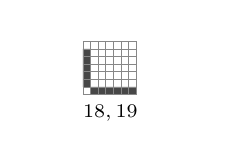
\begin{tikzpicture}[x=1mm,y=1mm,baseline=0mm]
\path[use as bounding box] (0,-.7) rectangle (21.5,11.9);
\begin{scope}[shift={(7.0,3.4)},x=0.97mm,y=0.97mm]
\fill[black!72] (0,5) rectangle (1,6) (0,4) rectangle (1,5) (0,3) rectangle (1,4) (0,2) rectangle (1,3) (0,1) rectangle (1,2) (1,0) rectangle (2,1) (2,0) rectangle (3,1) (3,0) rectangle (4,1) (4,0) rectangle (5,1) (5,0) rectangle (6,1) (6,0) rectangle (7,1);
\draw[black!47,line width=.16pt] (0,0)--(0,7) (0,0)--(7,0) (1,0)--(1,7) (0,1)--(7,1) (2,0)--(2,7) (0,2)--(7,2) (3,0)--(3,7) (0,3)--(7,3) (4,0)--(4,7) (0,4)--(7,4) (5,0)--(5,7) (0,5)--(7,5) (6,0)--(6,7) (0,6)--(7,6) (7,0)--(7,7) (0,7)--(7,7);
\end{scope}
\node[inner sep=0pt,font=\scriptsize] at (10.5,1.1) {$18,19$};
\end{tikzpicture} &
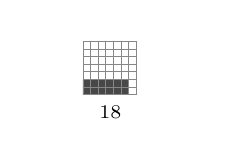
\begin{tikzpicture}[x=1mm,y=1mm,baseline=0mm]
\path[use as bounding box] (0,-.7) rectangle (21.5,11.9);
\begin{scope}[shift={(7.0,3.4)},x=0.97mm,y=0.97mm]
\fill[black!72] (0,1) rectangle (1,2) (1,1) rectangle (2,2) (2,1) rectangle (3,2) (3,1) rectangle (4,2) (4,1) rectangle (5,2) (5,1) rectangle (6,2) (0,0) rectangle (1,1) (1,0) rectangle (2,1) (2,0) rectangle (3,1) (3,0) rectangle (4,1) (4,0) rectangle (5,1) (5,0) rectangle (6,1);
\draw[black!47,line width=.16pt] (0,0)--(0,7) (0,0)--(7,0) (1,0)--(1,7) (0,1)--(7,1) (2,0)--(2,7) (0,2)--(7,2) (3,0)--(3,7) (0,3)--(7,3) (4,0)--(4,7) (0,4)--(7,4) (5,0)--(5,7) (0,5)--(7,5) (6,0)--(6,7) (0,6)--(7,6) (7,0)--(7,7) (0,7)--(7,7);
\end{scope}
\node[inner sep=0pt,font=\scriptsize] at (10.5,1.1) {$18$};
\end{tikzpicture} &
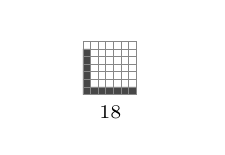
\begin{tikzpicture}[x=1mm,y=1mm,baseline=0mm]
\path[use as bounding box] (0,-.7) rectangle (21.5,11.9);
\begin{scope}[shift={(7.0,3.4)},x=0.97mm,y=0.97mm]
\fill[black!72] (0,5) rectangle (1,6) (0,4) rectangle (1,5) (0,3) rectangle (1,4) (0,2) rectangle (1,3) (0,1) rectangle (1,2) (0,0) rectangle (1,1) (1,0) rectangle (2,1) (2,0) rectangle (3,1) (3,0) rectangle (4,1) (4,0) rectangle (5,1) (5,0) rectangle (6,1) (6,0) rectangle (7,1);
\draw[black!47,line width=.16pt] (0,0)--(0,7) (0,0)--(7,0) (1,0)--(1,7) (0,1)--(7,1) (2,0)--(2,7) (0,2)--(7,2) (3,0)--(3,7) (0,3)--(7,3) (4,0)--(4,7) (0,4)--(7,4) (5,0)--(5,7) (0,5)--(7,5) (6,0)--(6,7) (0,6)--(7,6) (7,0)--(7,7) (0,7)--(7,7);
\end{scope}
\node[inner sep=0pt,font=\scriptsize] at (10.5,1.1) {$18$};
\end{tikzpicture} &
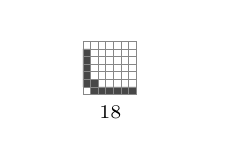
\begin{tikzpicture}[x=1mm,y=1mm,baseline=0mm]
\path[use as bounding box] (0,-.7) rectangle (21.5,11.9);
\begin{scope}[shift={(7.0,3.4)},x=0.97mm,y=0.97mm]
\fill[black!72] (0,5) rectangle (1,6) (0,4) rectangle (1,5) (0,3) rectangle (1,4) (0,2) rectangle (1,3) (0,1) rectangle (1,2) (1,1) rectangle (2,2) (1,0) rectangle (2,1) (2,0) rectangle (3,1) (3,0) rectangle (4,1) (4,0) rectangle (5,1) (5,0) rectangle (6,1) (6,0) rectangle (7,1);
\draw[black!47,line width=.16pt] (0,0)--(0,7) (0,0)--(7,0) (1,0)--(1,7) (0,1)--(7,1) (2,0)--(2,7) (0,2)--(7,2) (3,0)--(3,7) (0,3)--(7,3) (4,0)--(4,7) (0,4)--(7,4) (5,0)--(5,7) (0,5)--(7,5) (6,0)--(6,7) (0,6)--(7,6) (7,0)--(7,7) (0,7)--(7,7);
\end{scope}
\node[inner sep=0pt,font=\scriptsize] at (10.5,1.1) {$18$};
\end{tikzpicture} &
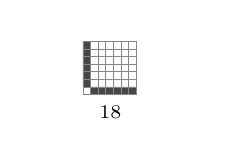
\begin{tikzpicture}[x=1mm,y=1mm,baseline=0mm]
\path[use as bounding box] (0,-.7) rectangle (21.5,11.9);
\begin{scope}[shift={(7.0,3.4)},x=0.97mm,y=0.97mm]
\fill[black!72] (0,6) rectangle (1,7) (0,5) rectangle (1,6) (0,4) rectangle (1,5) (0,3) rectangle (1,4) (0,2) rectangle (1,3) (0,1) rectangle (1,2) (1,0) rectangle (2,1) (2,0) rectangle (3,1) (3,0) rectangle (4,1) (4,0) rectangle (5,1) (5,0) rectangle (6,1) (6,0) rectangle (7,1);
\draw[black!47,line width=.16pt] (0,0)--(0,7) (0,0)--(7,0) (1,0)--(1,7) (0,1)--(7,1) (2,0)--(2,7) (0,2)--(7,2) (3,0)--(3,7) (0,3)--(7,3) (4,0)--(4,7) (0,4)--(7,4) (5,0)--(5,7) (0,5)--(7,5) (6,0)--(6,7) (0,6)--(7,6) (7,0)--(7,7) (0,7)--(7,7);
\end{scope}
\node[inner sep=0pt,font=\scriptsize] at (10.5,1.1) {$18$};
\end{tikzpicture} \\[.4mm]
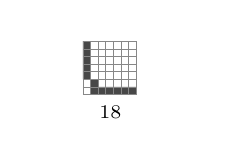
\begin{tikzpicture}[x=1mm,y=1mm,baseline=0mm]
\path[use as bounding box] (0,-.7) rectangle (21.5,11.9);
\begin{scope}[shift={(7.0,3.4)},x=0.97mm,y=0.97mm]
\fill[black!72] (0,6) rectangle (1,7) (0,5) rectangle (1,6) (0,4) rectangle (1,5) (0,3) rectangle (1,4) (0,2) rectangle (1,3) (1,1) rectangle (2,2) (1,0) rectangle (2,1) (2,0) rectangle (3,1) (3,0) rectangle (4,1) (4,0) rectangle (5,1) (5,0) rectangle (6,1) (6,0) rectangle (7,1);
\draw[black!47,line width=.16pt] (0,0)--(0,7) (0,0)--(7,0) (1,0)--(1,7) (0,1)--(7,1) (2,0)--(2,7) (0,2)--(7,2) (3,0)--(3,7) (0,3)--(7,3) (4,0)--(4,7) (0,4)--(7,4) (5,0)--(5,7) (0,5)--(7,5) (6,0)--(6,7) (0,6)--(7,6) (7,0)--(7,7) (0,7)--(7,7);
\end{scope}
\node[inner sep=0pt,font=\scriptsize] at (10.5,1.1) {$18$};
\end{tikzpicture} &
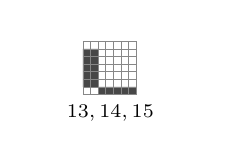
\begin{tikzpicture}[x=1mm,y=1mm,baseline=0mm]
\path[use as bounding box] (0,-.7) rectangle (21.5,11.9);
\begin{scope}[shift={(7.0,3.4)},x=0.97mm,y=0.97mm]
\fill[black!72] (0,5) rectangle (1,6) (1,5) rectangle (2,6) (0,4) rectangle (1,5) (1,4) rectangle (2,5) (0,3) rectangle (1,4) (1,3) rectangle (2,4) (0,2) rectangle (1,3) (1,2) rectangle (2,3) (0,1) rectangle (1,2) (1,1) rectangle (2,2) (2,0) rectangle (3,1) (3,0) rectangle (4,1) (4,0) rectangle (5,1) (5,0) rectangle (6,1) (6,0) rectangle (7,1);
\draw[black!47,line width=.16pt] (0,0)--(0,7) (0,0)--(7,0) (1,0)--(1,7) (0,1)--(7,1) (2,0)--(2,7) (0,2)--(7,2) (3,0)--(3,7) (0,3)--(7,3) (4,0)--(4,7) (0,4)--(7,4) (5,0)--(5,7) (0,5)--(7,5) (6,0)--(6,7) (0,6)--(7,6) (7,0)--(7,7) (0,7)--(7,7);
\end{scope}
\node[inner sep=0pt,font=\scriptsize] at (10.5,1.1) {$13,14,15$};
\end{tikzpicture} &
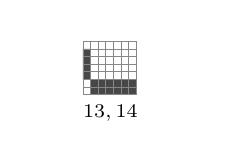
\begin{tikzpicture}[x=1mm,y=1mm,baseline=0mm]
\path[use as bounding box] (0,-.7) rectangle (21.5,11.9);
\begin{scope}[shift={(7.0,3.4)},x=0.97mm,y=0.97mm]
\fill[black!72] (0,5) rectangle (1,6) (0,4) rectangle (1,5) (0,3) rectangle (1,4) (0,2) rectangle (1,3) (1,1) rectangle (2,2) (2,1) rectangle (3,2) (3,1) rectangle (4,2) (4,1) rectangle (5,2) (5,1) rectangle (6,2) (6,1) rectangle (7,2) (1,0) rectangle (2,1) (2,0) rectangle (3,1) (3,0) rectangle (4,1) (4,0) rectangle (5,1) (5,0) rectangle (6,1) (6,0) rectangle (7,1);
\draw[black!47,line width=.16pt] (0,0)--(0,7) (0,0)--(7,0) (1,0)--(1,7) (0,1)--(7,1) (2,0)--(2,7) (0,2)--(7,2) (3,0)--(3,7) (0,3)--(7,3) (4,0)--(4,7) (0,4)--(7,4) (5,0)--(5,7) (0,5)--(7,5) (6,0)--(6,7) (0,6)--(7,6) (7,0)--(7,7) (0,7)--(7,7);
\end{scope}
\node[inner sep=0pt,font=\scriptsize] at (10.5,1.1) {$13,14$};
\end{tikzpicture} &
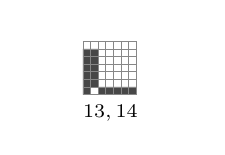
\begin{tikzpicture}[x=1mm,y=1mm,baseline=0mm]
\path[use as bounding box] (0,-.7) rectangle (21.5,11.9);
\begin{scope}[shift={(7.0,3.4)},x=0.97mm,y=0.97mm]
\fill[black!72] (0,5) rectangle (1,6) (1,5) rectangle (2,6) (0,4) rectangle (1,5) (1,4) rectangle (2,5) (0,3) rectangle (1,4) (1,3) rectangle (2,4) (0,2) rectangle (1,3) (1,2) rectangle (2,3) (0,1) rectangle (1,2) (1,1) rectangle (2,2) (0,0) rectangle (1,1) (2,0) rectangle (3,1) (3,0) rectangle (4,1) (4,0) rectangle (5,1) (5,0) rectangle (6,1) (6,0) rectangle (7,1);
\draw[black!47,line width=.16pt] (0,0)--(0,7) (0,0)--(7,0) (1,0)--(1,7) (0,1)--(7,1) (2,0)--(2,7) (0,2)--(7,2) (3,0)--(3,7) (0,3)--(7,3) (4,0)--(4,7) (0,4)--(7,4) (5,0)--(5,7) (0,5)--(7,5) (6,0)--(6,7) (0,6)--(7,6) (7,0)--(7,7) (0,7)--(7,7);
\end{scope}
\node[inner sep=0pt,font=\scriptsize] at (10.5,1.1) {$13,14$};
\end{tikzpicture} &
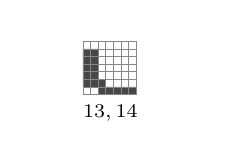
\begin{tikzpicture}[x=1mm,y=1mm,baseline=0mm]
\path[use as bounding box] (0,-.7) rectangle (21.5,11.9);
\begin{scope}[shift={(7.0,3.4)},x=0.97mm,y=0.97mm]
\fill[black!72] (0,5) rectangle (1,6) (1,5) rectangle (2,6) (0,4) rectangle (1,5) (1,4) rectangle (2,5) (0,3) rectangle (1,4) (1,3) rectangle (2,4) (0,2) rectangle (1,3) (1,2) rectangle (2,3) (0,1) rectangle (1,2) (1,1) rectangle (2,2) (2,1) rectangle (3,2) (2,0) rectangle (3,1) (3,0) rectangle (4,1) (4,0) rectangle (5,1) (5,0) rectangle (6,1) (6,0) rectangle (7,1);
\draw[black!47,line width=.16pt] (0,0)--(0,7) (0,0)--(7,0) (1,0)--(1,7) (0,1)--(7,1) (2,0)--(2,7) (0,2)--(7,2) (3,0)--(3,7) (0,3)--(7,3) (4,0)--(4,7) (0,4)--(7,4) (5,0)--(5,7) (0,5)--(7,5) (6,0)--(6,7) (0,6)--(7,6) (7,0)--(7,7) (0,7)--(7,7);
\end{scope}
\node[inner sep=0pt,font=\scriptsize] at (10.5,1.1) {$13,14$};
\end{tikzpicture} \\[.4mm]
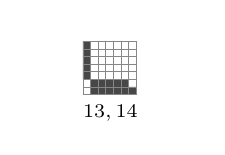
\begin{tikzpicture}[x=1mm,y=1mm,baseline=0mm]
\path[use as bounding box] (0,-.7) rectangle (21.5,11.9);
\begin{scope}[shift={(7.0,3.4)},x=0.97mm,y=0.97mm]
\fill[black!72] (0,6) rectangle (1,7) (0,5) rectangle (1,6) (0,4) rectangle (1,5) (0,3) rectangle (1,4) (0,2) rectangle (1,3) (1,1) rectangle (2,2) (2,1) rectangle (3,2) (3,1) rectangle (4,2) (4,1) rectangle (5,2) (5,1) rectangle (6,2) (1,0) rectangle (2,1) (2,0) rectangle (3,1) (3,0) rectangle (4,1) (4,0) rectangle (5,1) (5,0) rectangle (6,1) (6,0) rectangle (7,1);
\draw[black!47,line width=.16pt] (0,0)--(0,7) (0,0)--(7,0) (1,0)--(1,7) (0,1)--(7,1) (2,0)--(2,7) (0,2)--(7,2) (3,0)--(3,7) (0,3)--(7,3) (4,0)--(4,7) (0,4)--(7,4) (5,0)--(5,7) (0,5)--(7,5) (6,0)--(6,7) (0,6)--(7,6) (7,0)--(7,7) (0,7)--(7,7);
\end{scope}
\node[inner sep=0pt,font=\scriptsize] at (10.5,1.1) {$13,14$};
\end{tikzpicture} &
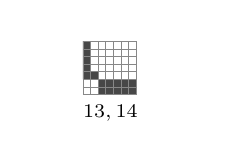
\begin{tikzpicture}[x=1mm,y=1mm,baseline=0mm]
\path[use as bounding box] (0,-.7) rectangle (21.5,11.9);
\begin{scope}[shift={(7.0,3.4)},x=0.97mm,y=0.97mm]
\fill[black!72] (0,6) rectangle (1,7) (0,5) rectangle (1,6) (0,4) rectangle (1,5) (0,3) rectangle (1,4) (0,2) rectangle (1,3) (1,2) rectangle (2,3) (2,1) rectangle (3,2) (3,1) rectangle (4,2) (4,1) rectangle (5,2) (5,1) rectangle (6,2) (6,1) rectangle (7,2) (2,0) rectangle (3,1) (3,0) rectangle (4,1) (4,0) rectangle (5,1) (5,0) rectangle (6,1) (6,0) rectangle (7,1);
\draw[black!47,line width=.16pt] (0,0)--(0,7) (0,0)--(7,0) (1,0)--(1,7) (0,1)--(7,1) (2,0)--(2,7) (0,2)--(7,2) (3,0)--(3,7) (0,3)--(7,3) (4,0)--(4,7) (0,4)--(7,4) (5,0)--(5,7) (0,5)--(7,5) (6,0)--(6,7) (0,6)--(7,6) (7,0)--(7,7) (0,7)--(7,7);
\end{scope}
\node[inner sep=0pt,font=\scriptsize] at (10.5,1.1) {$13,14$};
\end{tikzpicture} &
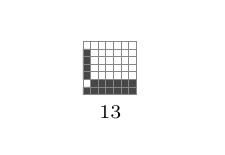
\begin{tikzpicture}[x=1mm,y=1mm,baseline=0mm]
\path[use as bounding box] (0,-.7) rectangle (21.5,11.9);
\begin{scope}[shift={(7.0,3.4)},x=0.97mm,y=0.97mm]
\fill[black!72] (0,5) rectangle (1,6) (0,4) rectangle (1,5) (0,3) rectangle (1,4) (0,2) rectangle (1,3) (1,1) rectangle (2,2) (2,1) rectangle (3,2) (3,1) rectangle (4,2) (4,1) rectangle (5,2) (5,1) rectangle (6,2) (6,1) rectangle (7,2) (0,0) rectangle (1,1) (1,0) rectangle (2,1) (2,0) rectangle (3,1) (3,0) rectangle (4,1) (4,0) rectangle (5,1) (5,0) rectangle (6,1) (6,0) rectangle (7,1);
\draw[black!47,line width=.16pt] (0,0)--(0,7) (0,0)--(7,0) (1,0)--(1,7) (0,1)--(7,1) (2,0)--(2,7) (0,2)--(7,2) (3,0)--(3,7) (0,3)--(7,3) (4,0)--(4,7) (0,4)--(7,4) (5,0)--(5,7) (0,5)--(7,5) (6,0)--(6,7) (0,6)--(7,6) (7,0)--(7,7) (0,7)--(7,7);
\end{scope}
\node[inner sep=0pt,font=\scriptsize] at (10.5,1.1) {$13$};
\end{tikzpicture} &
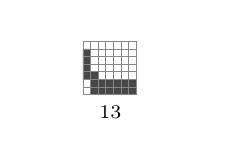
\begin{tikzpicture}[x=1mm,y=1mm,baseline=0mm]
\path[use as bounding box] (0,-.7) rectangle (21.5,11.9);
\begin{scope}[shift={(7.0,3.4)},x=0.97mm,y=0.97mm]
\fill[black!72] (0,5) rectangle (1,6) (0,4) rectangle (1,5) (0,3) rectangle (1,4) (0,2) rectangle (1,3) (1,2) rectangle (2,3) (1,1) rectangle (2,2) (2,1) rectangle (3,2) (3,1) rectangle (4,2) (4,1) rectangle (5,2) (5,1) rectangle (6,2) (6,1) rectangle (7,2) (1,0) rectangle (2,1) (2,0) rectangle (3,1) (3,0) rectangle (4,1) (4,0) rectangle (5,1) (5,0) rectangle (6,1) (6,0) rectangle (7,1);
\draw[black!47,line width=.16pt] (0,0)--(0,7) (0,0)--(7,0) (1,0)--(1,7) (0,1)--(7,1) (2,0)--(2,7) (0,2)--(7,2) (3,0)--(3,7) (0,3)--(7,3) (4,0)--(4,7) (0,4)--(7,4) (5,0)--(5,7) (0,5)--(7,5) (6,0)--(6,7) (0,6)--(7,6) (7,0)--(7,7) (0,7)--(7,7);
\end{scope}
\node[inner sep=0pt,font=\scriptsize] at (10.5,1.1) {$13$};
\end{tikzpicture} &
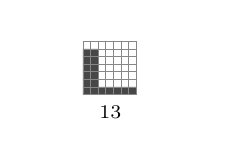
\begin{tikzpicture}[x=1mm,y=1mm,baseline=0mm]
\path[use as bounding box] (0,-.7) rectangle (21.5,11.9);
\begin{scope}[shift={(7.0,3.4)},x=0.97mm,y=0.97mm]
\fill[black!72] (0,5) rectangle (1,6) (1,5) rectangle (2,6) (0,4) rectangle (1,5) (1,4) rectangle (2,5) (0,3) rectangle (1,4) (1,3) rectangle (2,4) (0,2) rectangle (1,3) (1,2) rectangle (2,3) (0,1) rectangle (1,2) (1,1) rectangle (2,2) (0,0) rectangle (1,1) (1,0) rectangle (2,1) (2,0) rectangle (3,1) (3,0) rectangle (4,1) (4,0) rectangle (5,1) (5,0) rectangle (6,1) (6,0) rectangle (7,1);
\draw[black!47,line width=.16pt] (0,0)--(0,7) (0,0)--(7,0) (1,0)--(1,7) (0,1)--(7,1) (2,0)--(2,7) (0,2)--(7,2) (3,0)--(3,7) (0,3)--(7,3) (4,0)--(4,7) (0,4)--(7,4) (5,0)--(5,7) (0,5)--(7,5) (6,0)--(6,7) (0,6)--(7,6) (7,0)--(7,7) (0,7)--(7,7);
\end{scope}
\node[inner sep=0pt,font=\scriptsize] at (10.5,1.1) {$13$};
\end{tikzpicture} \\[.4mm]
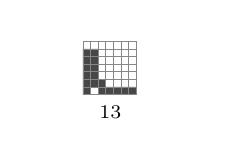
\begin{tikzpicture}[x=1mm,y=1mm,baseline=0mm]
\path[use as bounding box] (0,-.7) rectangle (21.5,11.9);
\begin{scope}[shift={(7.0,3.4)},x=0.97mm,y=0.97mm]
\fill[black!72] (0,5) rectangle (1,6) (1,5) rectangle (2,6) (0,4) rectangle (1,5) (1,4) rectangle (2,5) (0,3) rectangle (1,4) (1,3) rectangle (2,4) (0,2) rectangle (1,3) (1,2) rectangle (2,3) (0,1) rectangle (1,2) (1,1) rectangle (2,2) (2,1) rectangle (3,2) (0,0) rectangle (1,1) (2,0) rectangle (3,1) (3,0) rectangle (4,1) (4,0) rectangle (5,1) (5,0) rectangle (6,1) (6,0) rectangle (7,1);
\draw[black!47,line width=.16pt] (0,0)--(0,7) (0,0)--(7,0) (1,0)--(1,7) (0,1)--(7,1) (2,0)--(2,7) (0,2)--(7,2) (3,0)--(3,7) (0,3)--(7,3) (4,0)--(4,7) (0,4)--(7,4) (5,0)--(5,7) (0,5)--(7,5) (6,0)--(6,7) (0,6)--(7,6) (7,0)--(7,7) (0,7)--(7,7);
\end{scope}
\node[inner sep=0pt,font=\scriptsize] at (10.5,1.1) {$13$};
\end{tikzpicture} &
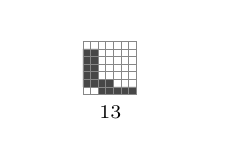
\begin{tikzpicture}[x=1mm,y=1mm,baseline=0mm]
\path[use as bounding box] (0,-.7) rectangle (21.5,11.9);
\begin{scope}[shift={(7.0,3.4)},x=0.97mm,y=0.97mm]
\fill[black!72] (0,5) rectangle (1,6) (1,5) rectangle (2,6) (0,4) rectangle (1,5) (1,4) rectangle (2,5) (0,3) rectangle (1,4) (1,3) rectangle (2,4) (0,2) rectangle (1,3) (1,2) rectangle (2,3) (0,1) rectangle (1,2) (1,1) rectangle (2,2) (2,1) rectangle (3,2) (3,1) rectangle (4,2) (2,0) rectangle (3,1) (3,0) rectangle (4,1) (4,0) rectangle (5,1) (5,0) rectangle (6,1) (6,0) rectangle (7,1);
\draw[black!47,line width=.16pt] (0,0)--(0,7) (0,0)--(7,0) (1,0)--(1,7) (0,1)--(7,1) (2,0)--(2,7) (0,2)--(7,2) (3,0)--(3,7) (0,3)--(7,3) (4,0)--(4,7) (0,4)--(7,4) (5,0)--(5,7) (0,5)--(7,5) (6,0)--(6,7) (0,6)--(7,6) (7,0)--(7,7) (0,7)--(7,7);
\end{scope}
\node[inner sep=0pt,font=\scriptsize] at (10.5,1.1) {$13$};
\end{tikzpicture} &
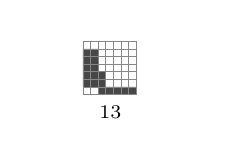
\begin{tikzpicture}[x=1mm,y=1mm,baseline=0mm]
\path[use as bounding box] (0,-.7) rectangle (21.5,11.9);
\begin{scope}[shift={(7.0,3.4)},x=0.97mm,y=0.97mm]
\fill[black!72] (0,5) rectangle (1,6) (1,5) rectangle (2,6) (0,4) rectangle (1,5) (1,4) rectangle (2,5) (0,3) rectangle (1,4) (1,3) rectangle (2,4) (0,2) rectangle (1,3) (1,2) rectangle (2,3) (2,2) rectangle (3,3) (0,1) rectangle (1,2) (1,1) rectangle (2,2) (2,1) rectangle (3,2) (2,0) rectangle (3,1) (3,0) rectangle (4,1) (4,0) rectangle (5,1) (5,0) rectangle (6,1) (6,0) rectangle (7,1);
\draw[black!47,line width=.16pt] (0,0)--(0,7) (0,0)--(7,0) (1,0)--(1,7) (0,1)--(7,1) (2,0)--(2,7) (0,2)--(7,2) (3,0)--(3,7) (0,3)--(7,3) (4,0)--(4,7) (0,4)--(7,4) (5,0)--(5,7) (0,5)--(7,5) (6,0)--(6,7) (0,6)--(7,6) (7,0)--(7,7) (0,7)--(7,7);
\end{scope}
\node[inner sep=0pt,font=\scriptsize] at (10.5,1.1) {$13$};
\end{tikzpicture} &
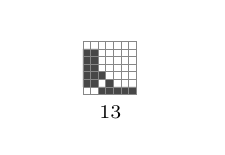
\begin{tikzpicture}[x=1mm,y=1mm,baseline=0mm]
\path[use as bounding box] (0,-.7) rectangle (21.5,11.9);
\begin{scope}[shift={(7.0,3.4)},x=0.97mm,y=0.97mm]
\fill[black!72] (0,5) rectangle (1,6) (1,5) rectangle (2,6) (0,4) rectangle (1,5) (1,4) rectangle (2,5) (0,3) rectangle (1,4) (1,3) rectangle (2,4) (0,2) rectangle (1,3) (1,2) rectangle (2,3) (2,2) rectangle (3,3) (0,1) rectangle (1,2) (1,1) rectangle (2,2) (3,1) rectangle (4,2) (2,0) rectangle (3,1) (3,0) rectangle (4,1) (4,0) rectangle (5,1) (5,0) rectangle (6,1) (6,0) rectangle (7,1);
\draw[black!47,line width=.16pt] (0,0)--(0,7) (0,0)--(7,0) (1,0)--(1,7) (0,1)--(7,1) (2,0)--(2,7) (0,2)--(7,2) (3,0)--(3,7) (0,3)--(7,3) (4,0)--(4,7) (0,4)--(7,4) (5,0)--(5,7) (0,5)--(7,5) (6,0)--(6,7) (0,6)--(7,6) (7,0)--(7,7) (0,7)--(7,7);
\end{scope}
\node[inner sep=0pt,font=\scriptsize] at (10.5,1.1) {$13$};
\end{tikzpicture} &
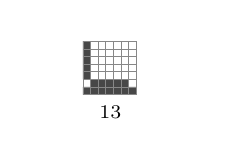
\begin{tikzpicture}[x=1mm,y=1mm,baseline=0mm]
\path[use as bounding box] (0,-.7) rectangle (21.5,11.9);
\begin{scope}[shift={(7.0,3.4)},x=0.97mm,y=0.97mm]
\fill[black!72] (0,6) rectangle (1,7) (0,5) rectangle (1,6) (0,4) rectangle (1,5) (0,3) rectangle (1,4) (0,2) rectangle (1,3) (1,1) rectangle (2,2) (2,1) rectangle (3,2) (3,1) rectangle (4,2) (4,1) rectangle (5,2) (5,1) rectangle (6,2) (0,0) rectangle (1,1) (1,0) rectangle (2,1) (2,0) rectangle (3,1) (3,0) rectangle (4,1) (4,0) rectangle (5,1) (5,0) rectangle (6,1) (6,0) rectangle (7,1);
\draw[black!47,line width=.16pt] (0,0)--(0,7) (0,0)--(7,0) (1,0)--(1,7) (0,1)--(7,1) (2,0)--(2,7) (0,2)--(7,2) (3,0)--(3,7) (0,3)--(7,3) (4,0)--(4,7) (0,4)--(7,4) (5,0)--(5,7) (0,5)--(7,5) (6,0)--(6,7) (0,6)--(7,6) (7,0)--(7,7) (0,7)--(7,7);
\end{scope}
\node[inner sep=0pt,font=\scriptsize] at (10.5,1.1) {$13$};
\end{tikzpicture} \\[.4mm]
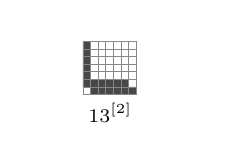
\begin{tikzpicture}[x=1mm,y=1mm,baseline=0mm]
\path[use as bounding box] (0,-.7) rectangle (21.5,11.9);
\begin{scope}[shift={(7.0,3.4)},x=0.97mm,y=0.97mm]
\fill[black!72] (0,6) rectangle (1,7) (0,5) rectangle (1,6) (0,4) rectangle (1,5) (0,3) rectangle (1,4) (0,2) rectangle (1,3) (0,1) rectangle (1,2) (1,1) rectangle (2,2) (2,1) rectangle (3,2) (3,1) rectangle (4,2) (4,1) rectangle (5,2) (5,1) rectangle (6,2) (1,0) rectangle (2,1) (2,0) rectangle (3,1) (3,0) rectangle (4,1) (4,0) rectangle (5,1) (5,0) rectangle (6,1) (6,0) rectangle (7,1);
\draw[black!47,line width=.16pt] (0,0)--(0,7) (0,0)--(7,0) (1,0)--(1,7) (0,1)--(7,1) (2,0)--(2,7) (0,2)--(7,2) (3,0)--(3,7) (0,3)--(7,3) (4,0)--(4,7) (0,4)--(7,4) (5,0)--(5,7) (0,5)--(7,5) (6,0)--(6,7) (0,6)--(7,6) (7,0)--(7,7) (0,7)--(7,7);
\end{scope}
\node[inner sep=0pt,font=\scriptsize] at (10.5,1.1) {$13^{[2]}$};
\end{tikzpicture} &
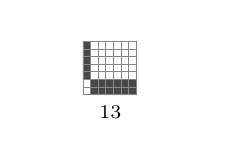
\begin{tikzpicture}[x=1mm,y=1mm,baseline=0mm]
\path[use as bounding box] (0,-.7) rectangle (21.5,11.9);
\begin{scope}[shift={(7.0,3.4)},x=0.97mm,y=0.97mm]
\fill[black!72] (0,6) rectangle (1,7) (0,5) rectangle (1,6) (0,4) rectangle (1,5) (0,3) rectangle (1,4) (0,2) rectangle (1,3) (1,1) rectangle (2,2) (2,1) rectangle (3,2) (3,1) rectangle (4,2) (4,1) rectangle (5,2) (5,1) rectangle (6,2) (6,1) rectangle (7,2) (1,0) rectangle (2,1) (2,0) rectangle (3,1) (3,0) rectangle (4,1) (4,0) rectangle (5,1) (5,0) rectangle (6,1) (6,0) rectangle (7,1);
\draw[black!47,line width=.16pt] (0,0)--(0,7) (0,0)--(7,0) (1,0)--(1,7) (0,1)--(7,1) (2,0)--(2,7) (0,2)--(7,2) (3,0)--(3,7) (0,3)--(7,3) (4,0)--(4,7) (0,4)--(7,4) (5,0)--(5,7) (0,5)--(7,5) (6,0)--(6,7) (0,6)--(7,6) (7,0)--(7,7) (0,7)--(7,7);
\end{scope}
\node[inner sep=0pt,font=\scriptsize] at (10.5,1.1) {$13$};
\end{tikzpicture} &
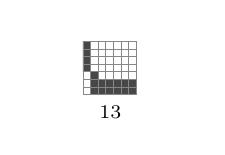
\begin{tikzpicture}[x=1mm,y=1mm,baseline=0mm]
\path[use as bounding box] (0,-.7) rectangle (21.5,11.9);
\begin{scope}[shift={(7.0,3.4)},x=0.97mm,y=0.97mm]
\fill[black!72] (0,6) rectangle (1,7) (0,5) rectangle (1,6) (0,4) rectangle (1,5) (0,3) rectangle (1,4) (1,2) rectangle (2,3) (1,1) rectangle (2,2) (2,1) rectangle (3,2) (3,1) rectangle (4,2) (4,1) rectangle (5,2) (5,1) rectangle (6,2) (6,1) rectangle (7,2) (1,0) rectangle (2,1) (2,0) rectangle (3,1) (3,0) rectangle (4,1) (4,0) rectangle (5,1) (5,0) rectangle (6,1) (6,0) rectangle (7,1);
\draw[black!47,line width=.16pt] (0,0)--(0,7) (0,0)--(7,0) (1,0)--(1,7) (0,1)--(7,1) (2,0)--(2,7) (0,2)--(7,2) (3,0)--(3,7) (0,3)--(7,3) (4,0)--(4,7) (0,4)--(7,4) (5,0)--(5,7) (0,5)--(7,5) (6,0)--(6,7) (0,6)--(7,6) (7,0)--(7,7) (0,7)--(7,7);
\end{scope}
\node[inner sep=0pt,font=\scriptsize] at (10.5,1.1) {$13$};
\end{tikzpicture} &
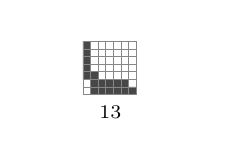
\begin{tikzpicture}[x=1mm,y=1mm,baseline=0mm]
\path[use as bounding box] (0,-.7) rectangle (21.5,11.9);
\begin{scope}[shift={(7.0,3.4)},x=0.97mm,y=0.97mm]
\fill[black!72] (0,6) rectangle (1,7) (0,5) rectangle (1,6) (0,4) rectangle (1,5) (0,3) rectangle (1,4) (0,2) rectangle (1,3) (1,2) rectangle (2,3) (1,1) rectangle (2,2) (2,1) rectangle (3,2) (3,1) rectangle (4,2) (4,1) rectangle (5,2) (5,1) rectangle (6,2) (1,0) rectangle (2,1) (2,0) rectangle (3,1) (3,0) rectangle (4,1) (4,0) rectangle (5,1) (5,0) rectangle (6,1) (6,0) rectangle (7,1);
\draw[black!47,line width=.16pt] (0,0)--(0,7) (0,0)--(7,0) (1,0)--(1,7) (0,1)--(7,1) (2,0)--(2,7) (0,2)--(7,2) (3,0)--(3,7) (0,3)--(7,3) (4,0)--(4,7) (0,4)--(7,4) (5,0)--(5,7) (0,5)--(7,5) (6,0)--(6,7) (0,6)--(7,6) (7,0)--(7,7) (0,7)--(7,7);
\end{scope}
\node[inner sep=0pt,font=\scriptsize] at (10.5,1.1) {$13$};
\end{tikzpicture} &
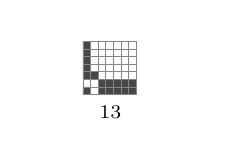
\begin{tikzpicture}[x=1mm,y=1mm,baseline=0mm]
\path[use as bounding box] (0,-.7) rectangle (21.5,11.9);
\begin{scope}[shift={(7.0,3.4)},x=0.97mm,y=0.97mm]
\fill[black!72] (0,6) rectangle (1,7) (0,5) rectangle (1,6) (0,4) rectangle (1,5) (0,3) rectangle (1,4) (0,2) rectangle (1,3) (1,2) rectangle (2,3) (2,1) rectangle (3,2) (3,1) rectangle (4,2) (4,1) rectangle (5,2) (5,1) rectangle (6,2) (6,1) rectangle (7,2) (0,0) rectangle (1,1) (2,0) rectangle (3,1) (3,0) rectangle (4,1) (4,0) rectangle (5,1) (5,0) rectangle (6,1) (6,0) rectangle (7,1);
\draw[black!47,line width=.16pt] (0,0)--(0,7) (0,0)--(7,0) (1,0)--(1,7) (0,1)--(7,1) (2,0)--(2,7) (0,2)--(7,2) (3,0)--(3,7) (0,3)--(7,3) (4,0)--(4,7) (0,4)--(7,4) (5,0)--(5,7) (0,5)--(7,5) (6,0)--(6,7) (0,6)--(7,6) (7,0)--(7,7) (0,7)--(7,7);
\end{scope}
\node[inner sep=0pt,font=\scriptsize] at (10.5,1.1) {$13$};
\end{tikzpicture} \\[.4mm]
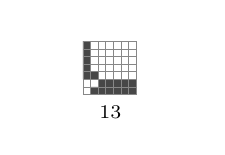
\begin{tikzpicture}[x=1mm,y=1mm,baseline=0mm]
\path[use as bounding box] (0,-.7) rectangle (21.5,11.9);
\begin{scope}[shift={(7.0,3.4)},x=0.97mm,y=0.97mm]
\fill[black!72] (0,6) rectangle (1,7) (0,5) rectangle (1,6) (0,4) rectangle (1,5) (0,3) rectangle (1,4) (0,2) rectangle (1,3) (1,2) rectangle (2,3) (2,1) rectangle (3,2) (3,1) rectangle (4,2) (4,1) rectangle (5,2) (5,1) rectangle (6,2) (6,1) rectangle (7,2) (1,0) rectangle (2,1) (2,0) rectangle (3,1) (3,0) rectangle (4,1) (4,0) rectangle (5,1) (5,0) rectangle (6,1) (6,0) rectangle (7,1);
\draw[black!47,line width=.16pt] (0,0)--(0,7) (0,0)--(7,0) (1,0)--(1,7) (0,1)--(7,1) (2,0)--(2,7) (0,2)--(7,2) (3,0)--(3,7) (0,3)--(7,3) (4,0)--(4,7) (0,4)--(7,4) (5,0)--(5,7) (0,5)--(7,5) (6,0)--(6,7) (0,6)--(7,6) (7,0)--(7,7) (0,7)--(7,7);
\end{scope}
\node[inner sep=0pt,font=\scriptsize] at (10.5,1.1) {$13$};
\end{tikzpicture} &
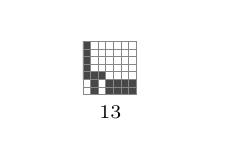
\begin{tikzpicture}[x=1mm,y=1mm,baseline=0mm]
\path[use as bounding box] (0,-.7) rectangle (21.5,11.9);
\begin{scope}[shift={(7.0,3.4)},x=0.97mm,y=0.97mm]
\fill[black!72] (0,6) rectangle (1,7) (0,5) rectangle (1,6) (0,4) rectangle (1,5) (0,3) rectangle (1,4) (0,2) rectangle (1,3) (1,2) rectangle (2,3) (2,2) rectangle (3,3) (1,1) rectangle (2,2) (3,1) rectangle (4,2) (4,1) rectangle (5,2) (5,1) rectangle (6,2) (6,1) rectangle (7,2) (1,0) rectangle (2,1) (3,0) rectangle (4,1) (4,0) rectangle (5,1) (5,0) rectangle (6,1) (6,0) rectangle (7,1);
\draw[black!47,line width=.16pt] (0,0)--(0,7) (0,0)--(7,0) (1,0)--(1,7) (0,1)--(7,1) (2,0)--(2,7) (0,2)--(7,2) (3,0)--(3,7) (0,3)--(7,3) (4,0)--(4,7) (0,4)--(7,4) (5,0)--(5,7) (0,5)--(7,5) (6,0)--(6,7) (0,6)--(7,6) (7,0)--(7,7) (0,7)--(7,7);
\end{scope}
\node[inner sep=0pt,font=\scriptsize] at (10.5,1.1) {$13$};
\end{tikzpicture} &
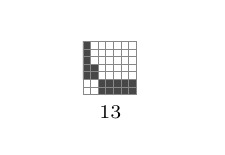
\begin{tikzpicture}[x=1mm,y=1mm,baseline=0mm]
\path[use as bounding box] (0,-.7) rectangle (21.5,11.9);
\begin{scope}[shift={(7.0,3.4)},x=0.97mm,y=0.97mm]
\fill[black!72] (0,6) rectangle (1,7) (0,5) rectangle (1,6) (0,4) rectangle (1,5) (0,3) rectangle (1,4) (1,3) rectangle (2,4) (0,2) rectangle (1,3) (1,2) rectangle (2,3) (2,1) rectangle (3,2) (3,1) rectangle (4,2) (4,1) rectangle (5,2) (5,1) rectangle (6,2) (6,1) rectangle (7,2) (2,0) rectangle (3,1) (3,0) rectangle (4,1) (4,0) rectangle (5,1) (5,0) rectangle (6,1) (6,0) rectangle (7,1);
\draw[black!47,line width=.16pt] (0,0)--(0,7) (0,0)--(7,0) (1,0)--(1,7) (0,1)--(7,1) (2,0)--(2,7) (0,2)--(7,2) (3,0)--(3,7) (0,3)--(7,3) (4,0)--(4,7) (0,4)--(7,4) (5,0)--(5,7) (0,5)--(7,5) (6,0)--(6,7) (0,6)--(7,6) (7,0)--(7,7) (0,7)--(7,7);
\end{scope}
\node[inner sep=0pt,font=\scriptsize] at (10.5,1.1) {$13$};
\end{tikzpicture} &
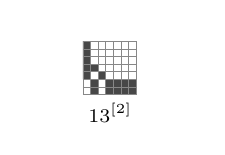
\begin{tikzpicture}[x=1mm,y=1mm,baseline=0mm]
\path[use as bounding box] (0,-.7) rectangle (21.5,11.9);
\begin{scope}[shift={(7.0,3.4)},x=0.97mm,y=0.97mm]
\fill[black!72] (0,6) rectangle (1,7) (0,5) rectangle (1,6) (0,4) rectangle (1,5) (0,3) rectangle (1,4) (1,3) rectangle (2,4) (0,2) rectangle (1,3) (2,2) rectangle (3,3) (1,1) rectangle (2,2) (3,1) rectangle (4,2) (4,1) rectangle (5,2) (5,1) rectangle (6,2) (6,1) rectangle (7,2) (1,0) rectangle (2,1) (3,0) rectangle (4,1) (4,0) rectangle (5,1) (5,0) rectangle (6,1) (6,0) rectangle (7,1);
\draw[black!47,line width=.16pt] (0,0)--(0,7) (0,0)--(7,0) (1,0)--(1,7) (0,1)--(7,1) (2,0)--(2,7) (0,2)--(7,2) (3,0)--(3,7) (0,3)--(7,3) (4,0)--(4,7) (0,4)--(7,4) (5,0)--(5,7) (0,5)--(7,5) (6,0)--(6,7) (0,6)--(7,6) (7,0)--(7,7) (0,7)--(7,7);
\end{scope}
\node[inner sep=0pt,font=\scriptsize] at (10.5,1.1) {$13^{[2]}$};
\end{tikzpicture} &
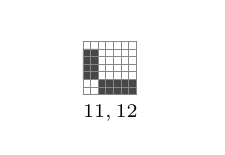
\begin{tikzpicture}[x=1mm,y=1mm,baseline=0mm]
\path[use as bounding box] (0,-.7) rectangle (21.5,11.9);
\begin{scope}[shift={(7.0,3.4)},x=0.97mm,y=0.97mm]
\fill[black!72] (0,5) rectangle (1,6) (1,5) rectangle (2,6) (0,4) rectangle (1,5) (1,4) rectangle (2,5) (0,3) rectangle (1,4) (1,3) rectangle (2,4) (0,2) rectangle (1,3) (1,2) rectangle (2,3) (2,1) rectangle (3,2) (3,1) rectangle (4,2) (4,1) rectangle (5,2) (5,1) rectangle (6,2) (6,1) rectangle (7,2) (2,0) rectangle (3,1) (3,0) rectangle (4,1) (4,0) rectangle (5,1) (5,0) rectangle (6,1) (6,0) rectangle (7,1);
\draw[black!47,line width=.16pt] (0,0)--(0,7) (0,0)--(7,0) (1,0)--(1,7) (0,1)--(7,1) (2,0)--(2,7) (0,2)--(7,2) (3,0)--(3,7) (0,3)--(7,3) (4,0)--(4,7) (0,4)--(7,4) (5,0)--(5,7) (0,5)--(7,5) (6,0)--(6,7) (0,6)--(7,6) (7,0)--(7,7) (0,7)--(7,7);
\end{scope}
\node[inner sep=0pt,font=\scriptsize] at (10.5,1.1) {$11,12$};
\end{tikzpicture} \\[.4mm]
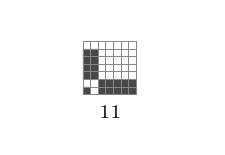
\begin{tikzpicture}[x=1mm,y=1mm,baseline=0mm]
\path[use as bounding box] (0,-.7) rectangle (21.5,11.9);
\begin{scope}[shift={(7.0,3.4)},x=0.97mm,y=0.97mm]
\fill[black!72] (0,5) rectangle (1,6) (1,5) rectangle (2,6) (0,4) rectangle (1,5) (1,4) rectangle (2,5) (0,3) rectangle (1,4) (1,3) rectangle (2,4) (0,2) rectangle (1,3) (1,2) rectangle (2,3) (2,1) rectangle (3,2) (3,1) rectangle (4,2) (4,1) rectangle (5,2) (5,1) rectangle (6,2) (6,1) rectangle (7,2) (0,0) rectangle (1,1) (2,0) rectangle (3,1) (3,0) rectangle (4,1) (4,0) rectangle (5,1) (5,0) rectangle (6,1) (6,0) rectangle (7,1);
\draw[black!47,line width=.16pt] (0,0)--(0,7) (0,0)--(7,0) (1,0)--(1,7) (0,1)--(7,1) (2,0)--(2,7) (0,2)--(7,2) (3,0)--(3,7) (0,3)--(7,3) (4,0)--(4,7) (0,4)--(7,4) (5,0)--(5,7) (0,5)--(7,5) (6,0)--(6,7) (0,6)--(7,6) (7,0)--(7,7) (0,7)--(7,7);
\end{scope}
\node[inner sep=0pt,font=\scriptsize] at (10.5,1.1) {$11$};
\end{tikzpicture} &
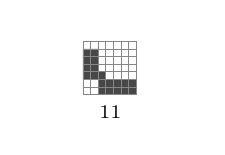
\begin{tikzpicture}[x=1mm,y=1mm,baseline=0mm]
\path[use as bounding box] (0,-.7) rectangle (21.5,11.9);
\begin{scope}[shift={(7.0,3.4)},x=0.97mm,y=0.97mm]
\fill[black!72] (0,5) rectangle (1,6) (1,5) rectangle (2,6) (0,4) rectangle (1,5) (1,4) rectangle (2,5) (0,3) rectangle (1,4) (1,3) rectangle (2,4) (0,2) rectangle (1,3) (1,2) rectangle (2,3) (2,2) rectangle (3,3) (2,1) rectangle (3,2) (3,1) rectangle (4,2) (4,1) rectangle (5,2) (5,1) rectangle (6,2) (6,1) rectangle (7,2) (2,0) rectangle (3,1) (3,0) rectangle (4,1) (4,0) rectangle (5,1) (5,0) rectangle (6,1) (6,0) rectangle (7,1);
\draw[black!47,line width=.16pt] (0,0)--(0,7) (0,0)--(7,0) (1,0)--(1,7) (0,1)--(7,1) (2,0)--(2,7) (0,2)--(7,2) (3,0)--(3,7) (0,3)--(7,3) (4,0)--(4,7) (0,4)--(7,4) (5,0)--(5,7) (0,5)--(7,5) (6,0)--(6,7) (0,6)--(7,6) (7,0)--(7,7) (0,7)--(7,7);
\end{scope}
\node[inner sep=0pt,font=\scriptsize] at (10.5,1.1) {$11$};
\end{tikzpicture} &
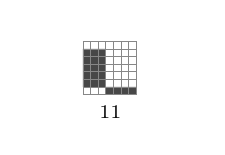
\begin{tikzpicture}[x=1mm,y=1mm,baseline=0mm]
\path[use as bounding box] (0,-.7) rectangle (21.5,11.9);
\begin{scope}[shift={(7.0,3.4)},x=0.97mm,y=0.97mm]
\fill[black!72] (0,5) rectangle (1,6) (1,5) rectangle (2,6) (2,5) rectangle (3,6) (0,4) rectangle (1,5) (1,4) rectangle (2,5) (2,4) rectangle (3,5) (0,3) rectangle (1,4) (1,3) rectangle (2,4) (2,3) rectangle (3,4) (0,2) rectangle (1,3) (1,2) rectangle (2,3) (2,2) rectangle (3,3) (0,1) rectangle (1,2) (1,1) rectangle (2,2) (2,1) rectangle (3,2) (3,0) rectangle (4,1) (4,0) rectangle (5,1) (5,0) rectangle (6,1) (6,0) rectangle (7,1);
\draw[black!47,line width=.16pt] (0,0)--(0,7) (0,0)--(7,0) (1,0)--(1,7) (0,1)--(7,1) (2,0)--(2,7) (0,2)--(7,2) (3,0)--(3,7) (0,3)--(7,3) (4,0)--(4,7) (0,4)--(7,4) (5,0)--(5,7) (0,5)--(7,5) (6,0)--(6,7) (0,6)--(7,6) (7,0)--(7,7) (0,7)--(7,7);
\end{scope}
\node[inner sep=0pt,font=\scriptsize] at (10.5,1.1) {$11$};
\end{tikzpicture} &
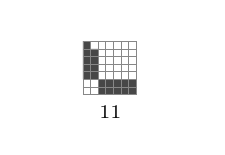
\begin{tikzpicture}[x=1mm,y=1mm,baseline=0mm]
\path[use as bounding box] (0,-.7) rectangle (21.5,11.9);
\begin{scope}[shift={(7.0,3.4)},x=0.97mm,y=0.97mm]
\fill[black!72] (0,6) rectangle (1,7) (0,5) rectangle (1,6) (1,5) rectangle (2,6) (0,4) rectangle (1,5) (1,4) rectangle (2,5) (0,3) rectangle (1,4) (1,3) rectangle (2,4) (0,2) rectangle (1,3) (1,2) rectangle (2,3) (2,1) rectangle (3,2) (3,1) rectangle (4,2) (4,1) rectangle (5,2) (5,1) rectangle (6,2) (6,1) rectangle (7,2) (2,0) rectangle (3,1) (3,0) rectangle (4,1) (4,0) rectangle (5,1) (5,0) rectangle (6,1) (6,0) rectangle (7,1);
\draw[black!47,line width=.16pt] (0,0)--(0,7) (0,0)--(7,0) (1,0)--(1,7) (0,1)--(7,1) (2,0)--(2,7) (0,2)--(7,2) (3,0)--(3,7) (0,3)--(7,3) (4,0)--(4,7) (0,4)--(7,4) (5,0)--(5,7) (0,5)--(7,5) (6,0)--(6,7) (0,6)--(7,6) (7,0)--(7,7) (0,7)--(7,7);
\end{scope}
\node[inner sep=0pt,font=\scriptsize] at (10.5,1.1) {$11$};
\end{tikzpicture} &
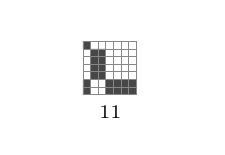
\begin{tikzpicture}[x=1mm,y=1mm,baseline=0mm]
\path[use as bounding box] (0,-.7) rectangle (21.5,11.9);
\begin{scope}[shift={(7.0,3.4)},x=0.97mm,y=0.97mm]
\fill[black!72] (0,6) rectangle (1,7) (1,5) rectangle (2,6) (2,5) rectangle (3,6) (1,4) rectangle (2,5) (2,4) rectangle (3,5) (1,3) rectangle (2,4) (2,3) rectangle (3,4) (1,2) rectangle (2,3) (2,2) rectangle (3,3) (0,1) rectangle (1,2) (3,1) rectangle (4,2) (4,1) rectangle (5,2) (5,1) rectangle (6,2) (6,1) rectangle (7,2) (0,0) rectangle (1,1) (3,0) rectangle (4,1) (4,0) rectangle (5,1) (5,0) rectangle (6,1) (6,0) rectangle (7,1);
\draw[black!47,line width=.16pt] (0,0)--(0,7) (0,0)--(7,0) (1,0)--(1,7) (0,1)--(7,1) (2,0)--(2,7) (0,2)--(7,2) (3,0)--(3,7) (0,3)--(7,3) (4,0)--(4,7) (0,4)--(7,4) (5,0)--(5,7) (0,5)--(7,5) (6,0)--(6,7) (0,6)--(7,6) (7,0)--(7,7) (0,7)--(7,7);
\end{scope}
\node[inner sep=0pt,font=\scriptsize] at (10.5,1.1) {$11$};
\end{tikzpicture} \\[.4mm]
\end{tabular}
\caption{Cross adjacencies tested in the connected case, part 1 of 2.}
\label{fig:nine-qfourteen-connected}
\end{figure}

\begin{figure}[!htbp]
\centering
\begin{tabular}{@{}c@{\hspace{1.6mm}}c@{\hspace{1.6mm}}c@{\hspace{1.6mm}}c@{\hspace{1.6mm}}c@{}}
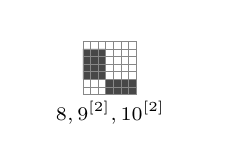
\begin{tikzpicture}[x=1mm,y=1mm,baseline=0mm]
\path[use as bounding box] (0,-.7) rectangle (21.5,11.9);
\begin{scope}[shift={(7.0,3.4)},x=0.97mm,y=0.97mm]
\fill[black!72] (0,5) rectangle (1,6) (1,5) rectangle (2,6) (2,5) rectangle (3,6) (0,4) rectangle (1,5) (1,4) rectangle (2,5) (2,4) rectangle (3,5) (0,3) rectangle (1,4) (1,3) rectangle (2,4) (2,3) rectangle (3,4) (0,2) rectangle (1,3) (1,2) rectangle (2,3) (2,2) rectangle (3,3) (3,1) rectangle (4,2) (4,1) rectangle (5,2) (5,1) rectangle (6,2) (6,1) rectangle (7,2) (3,0) rectangle (4,1) (4,0) rectangle (5,1) (5,0) rectangle (6,1) (6,0) rectangle (7,1);
\draw[black!47,line width=.16pt] (0,0)--(0,7) (0,0)--(7,0) (1,0)--(1,7) (0,1)--(7,1) (2,0)--(2,7) (0,2)--(7,2) (3,0)--(3,7) (0,3)--(7,3) (4,0)--(4,7) (0,4)--(7,4) (5,0)--(5,7) (0,5)--(7,5) (6,0)--(6,7) (0,6)--(7,6) (7,0)--(7,7) (0,7)--(7,7);
\end{scope}
\node[inner sep=0pt,font=\scriptsize] at (10.5,1.1) {$8,9^{[2]},10^{[2]}$};
\end{tikzpicture} &
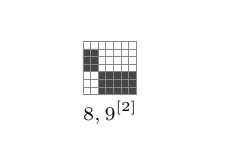
\begin{tikzpicture}[x=1mm,y=1mm,baseline=0mm]
\path[use as bounding box] (0,-.7) rectangle (21.5,11.9);
\begin{scope}[shift={(7.0,3.4)},x=0.97mm,y=0.97mm]
\fill[black!72] (0,5) rectangle (1,6) (1,5) rectangle (2,6) (0,4) rectangle (1,5) (1,4) rectangle (2,5) (0,3) rectangle (1,4) (1,3) rectangle (2,4) (2,2) rectangle (3,3) (3,2) rectangle (4,3) (4,2) rectangle (5,3) (5,2) rectangle (6,3) (6,2) rectangle (7,3) (2,1) rectangle (3,2) (3,1) rectangle (4,2) (4,1) rectangle (5,2) (5,1) rectangle (6,2) (6,1) rectangle (7,2) (2,0) rectangle (3,1) (3,0) rectangle (4,1) (4,0) rectangle (5,1) (5,0) rectangle (6,1) (6,0) rectangle (7,1);
\draw[black!47,line width=.16pt] (0,0)--(0,7) (0,0)--(7,0) (1,0)--(1,7) (0,1)--(7,1) (2,0)--(2,7) (0,2)--(7,2) (3,0)--(3,7) (0,3)--(7,3) (4,0)--(4,7) (0,4)--(7,4) (5,0)--(5,7) (0,5)--(7,5) (6,0)--(6,7) (0,6)--(7,6) (7,0)--(7,7) (0,7)--(7,7);
\end{scope}
\node[inner sep=0pt,font=\scriptsize] at (10.5,1.1) {$8,9^{[2]}$};
\end{tikzpicture} &
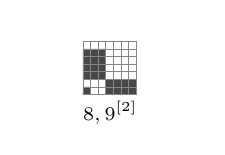
\begin{tikzpicture}[x=1mm,y=1mm,baseline=0mm]
\path[use as bounding box] (0,-.7) rectangle (21.5,11.9);
\begin{scope}[shift={(7.0,3.4)},x=0.97mm,y=0.97mm]
\fill[black!72] (0,5) rectangle (1,6) (1,5) rectangle (2,6) (2,5) rectangle (3,6) (0,4) rectangle (1,5) (1,4) rectangle (2,5) (2,4) rectangle (3,5) (0,3) rectangle (1,4) (1,3) rectangle (2,4) (2,3) rectangle (3,4) (0,2) rectangle (1,3) (1,2) rectangle (2,3) (2,2) rectangle (3,3) (3,1) rectangle (4,2) (4,1) rectangle (5,2) (5,1) rectangle (6,2) (6,1) rectangle (7,2) (0,0) rectangle (1,1) (3,0) rectangle (4,1) (4,0) rectangle (5,1) (5,0) rectangle (6,1) (6,0) rectangle (7,1);
\draw[black!47,line width=.16pt] (0,0)--(0,7) (0,0)--(7,0) (1,0)--(1,7) (0,1)--(7,1) (2,0)--(2,7) (0,2)--(7,2) (3,0)--(3,7) (0,3)--(7,3) (4,0)--(4,7) (0,4)--(7,4) (5,0)--(5,7) (0,5)--(7,5) (6,0)--(6,7) (0,6)--(7,6) (7,0)--(7,7) (0,7)--(7,7);
\end{scope}
\node[inner sep=0pt,font=\scriptsize] at (10.5,1.1) {$8,9^{[2]}$};
\end{tikzpicture} &
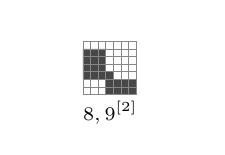
\begin{tikzpicture}[x=1mm,y=1mm,baseline=0mm]
\path[use as bounding box] (0,-.7) rectangle (21.5,11.9);
\begin{scope}[shift={(7.0,3.4)},x=0.97mm,y=0.97mm]
\fill[black!72] (0,5) rectangle (1,6) (1,5) rectangle (2,6) (2,5) rectangle (3,6) (0,4) rectangle (1,5) (1,4) rectangle (2,5) (2,4) rectangle (3,5) (0,3) rectangle (1,4) (1,3) rectangle (2,4) (2,3) rectangle (3,4) (0,2) rectangle (1,3) (1,2) rectangle (2,3) (2,2) rectangle (3,3) (3,2) rectangle (4,3) (3,1) rectangle (4,2) (4,1) rectangle (5,2) (5,1) rectangle (6,2) (6,1) rectangle (7,2) (3,0) rectangle (4,1) (4,0) rectangle (5,1) (5,0) rectangle (6,1) (6,0) rectangle (7,1);
\draw[black!47,line width=.16pt] (0,0)--(0,7) (0,0)--(7,0) (1,0)--(1,7) (0,1)--(7,1) (2,0)--(2,7) (0,2)--(7,2) (3,0)--(3,7) (0,3)--(7,3) (4,0)--(4,7) (0,4)--(7,4) (5,0)--(5,7) (0,5)--(7,5) (6,0)--(6,7) (0,6)--(7,6) (7,0)--(7,7) (0,7)--(7,7);
\end{scope}
\node[inner sep=0pt,font=\scriptsize] at (10.5,1.1) {$8,9^{[2]}$};
\end{tikzpicture} &
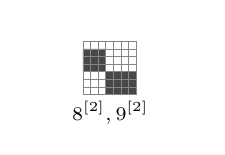
\begin{tikzpicture}[x=1mm,y=1mm,baseline=0mm]
\path[use as bounding box] (0,-.7) rectangle (21.5,11.9);
\begin{scope}[shift={(7.0,3.4)},x=0.97mm,y=0.97mm]
\fill[black!72] (0,5) rectangle (1,6) (1,5) rectangle (2,6) (2,5) rectangle (3,6) (0,4) rectangle (1,5) (1,4) rectangle (2,5) (2,4) rectangle (3,5) (0,3) rectangle (1,4) (1,3) rectangle (2,4) (2,3) rectangle (3,4) (3,2) rectangle (4,3) (4,2) rectangle (5,3) (5,2) rectangle (6,3) (6,2) rectangle (7,3) (3,1) rectangle (4,2) (4,1) rectangle (5,2) (5,1) rectangle (6,2) (6,1) rectangle (7,2) (3,0) rectangle (4,1) (4,0) rectangle (5,1) (5,0) rectangle (6,1) (6,0) rectangle (7,1);
\draw[black!47,line width=.16pt] (0,0)--(0,7) (0,0)--(7,0) (1,0)--(1,7) (0,1)--(7,1) (2,0)--(2,7) (0,2)--(7,2) (3,0)--(3,7) (0,3)--(7,3) (4,0)--(4,7) (0,4)--(7,4) (5,0)--(5,7) (0,5)--(7,5) (6,0)--(6,7) (0,6)--(7,6) (7,0)--(7,7) (0,7)--(7,7);
\end{scope}
\node[inner sep=0pt,font=\scriptsize] at (10.5,1.1) {$8^{[2]},9^{[2]}$};
\end{tikzpicture} \\[.4mm]
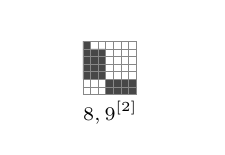
\begin{tikzpicture}[x=1mm,y=1mm,baseline=0mm]
\path[use as bounding box] (0,-.7) rectangle (21.5,11.9);
\begin{scope}[shift={(7.0,3.4)},x=0.97mm,y=0.97mm]
\fill[black!72] (0,6) rectangle (1,7) (0,5) rectangle (1,6) (1,5) rectangle (2,6) (2,5) rectangle (3,6) (0,4) rectangle (1,5) (1,4) rectangle (2,5) (2,4) rectangle (3,5) (0,3) rectangle (1,4) (1,3) rectangle (2,4) (2,3) rectangle (3,4) (0,2) rectangle (1,3) (1,2) rectangle (2,3) (2,2) rectangle (3,3) (3,1) rectangle (4,2) (4,1) rectangle (5,2) (5,1) rectangle (6,2) (6,1) rectangle (7,2) (3,0) rectangle (4,1) (4,0) rectangle (5,1) (5,0) rectangle (6,1) (6,0) rectangle (7,1);
\draw[black!47,line width=.16pt] (0,0)--(0,7) (0,0)--(7,0) (1,0)--(1,7) (0,1)--(7,1) (2,0)--(2,7) (0,2)--(7,2) (3,0)--(3,7) (0,3)--(7,3) (4,0)--(4,7) (0,4)--(7,4) (5,0)--(5,7) (0,5)--(7,5) (6,0)--(6,7) (0,6)--(7,6) (7,0)--(7,7) (0,7)--(7,7);
\end{scope}
\node[inner sep=0pt,font=\scriptsize] at (10.5,1.1) {$8,9^{[2]}$};
\end{tikzpicture} &
\begin{tikzpicture}[x=1mm,y=1mm,baseline=0mm]
\path[use as bounding box] (0,-.7) rectangle (21.5,11.9);
\begin{scope}[shift={(7.0,3.4)},x=0.97mm,y=0.97mm]
\fill[black!72] (0,6) rectangle (1,7) (1,5) rectangle (2,6) (2,5) rectangle (3,6) (3,5) rectangle (4,6) (1,4) rectangle (2,5) (2,4) rectangle (3,5) (3,4) rectangle (4,5) (1,3) rectangle (2,4) (2,3) rectangle (3,4) (3,3) rectangle (4,4) (1,2) rectangle (2,3) (2,2) rectangle (3,3) (3,2) rectangle (4,3) (0,1) rectangle (1,2) (4,1) rectangle (5,2) (5,1) rectangle (6,2) (6,1) rectangle (7,2) (0,0) rectangle (1,1) (4,0) rectangle (5,1) (5,0) rectangle (6,1) (6,0) rectangle (7,1);
\draw[black!47,line width=.16pt] (0,0)--(0,7) (0,0)--(7,0) (1,0)--(1,7) (0,1)--(7,1) (2,0)--(2,7) (0,2)--(7,2) (3,0)--(3,7) (0,3)--(7,3) (4,0)--(4,7) (0,4)--(7,4) (5,0)--(5,7) (0,5)--(7,5) (6,0)--(6,7) (0,6)--(7,6) (7,0)--(7,7) (0,7)--(7,7);
\end{scope}
\node[inner sep=0pt,font=\scriptsize] at (10.5,1.1) {$8,9^{[2]}$};
\end{tikzpicture} &
\begin{tikzpicture}[x=1mm,y=1mm,baseline=0mm]
\path[use as bounding box] (0,-.7) rectangle (21.5,11.9);
\begin{scope}[shift={(7.0,3.4)},x=0.97mm,y=0.97mm]
\fill[black!72] (0,5) rectangle (1,6) (1,5) rectangle (2,6) (0,4) rectangle (1,5) (1,4) rectangle (2,5) (0,3) rectangle (1,4) (1,3) rectangle (2,4) (2,2) rectangle (3,3) (3,2) rectangle (4,3) (4,2) rectangle (5,3) (5,2) rectangle (6,3) (6,2) rectangle (7,3) (2,1) rectangle (3,2) (3,1) rectangle (4,2) (4,1) rectangle (5,2) (5,1) rectangle (6,2) (6,1) rectangle (7,2) (0,0) rectangle (1,1) (2,0) rectangle (3,1) (3,0) rectangle (4,1) (4,0) rectangle (5,1) (5,0) rectangle (6,1) (6,0) rectangle (7,1);
\draw[black!47,line width=.16pt] (0,0)--(0,7) (0,0)--(7,0) (1,0)--(1,7) (0,1)--(7,1) (2,0)--(2,7) (0,2)--(7,2) (3,0)--(3,7) (0,3)--(7,3) (4,0)--(4,7) (0,4)--(7,4) (5,0)--(5,7) (0,5)--(7,5) (6,0)--(6,7) (0,6)--(7,6) (7,0)--(7,7) (0,7)--(7,7);
\end{scope}
\node[inner sep=0pt,font=\scriptsize] at (10.5,1.1) {$8$};
\end{tikzpicture} &
\begin{tikzpicture}[x=1mm,y=1mm,baseline=0mm]
\path[use as bounding box] (0,-.7) rectangle (21.5,11.9);
\begin{scope}[shift={(7.0,3.4)},x=0.97mm,y=0.97mm]
\fill[black!72] (0,5) rectangle (1,6) (1,5) rectangle (2,6) (0,4) rectangle (1,5) (1,4) rectangle (2,5) (0,3) rectangle (1,4) (1,3) rectangle (2,4) (2,3) rectangle (3,4) (2,2) rectangle (3,3) (3,2) rectangle (4,3) (4,2) rectangle (5,3) (5,2) rectangle (6,3) (6,2) rectangle (7,3) (2,1) rectangle (3,2) (3,1) rectangle (4,2) (4,1) rectangle (5,2) (5,1) rectangle (6,2) (6,1) rectangle (7,2) (2,0) rectangle (3,1) (3,0) rectangle (4,1) (4,0) rectangle (5,1) (5,0) rectangle (6,1) (6,0) rectangle (7,1);
\draw[black!47,line width=.16pt] (0,0)--(0,7) (0,0)--(7,0) (1,0)--(1,7) (0,1)--(7,1) (2,0)--(2,7) (0,2)--(7,2) (3,0)--(3,7) (0,3)--(7,3) (4,0)--(4,7) (0,4)--(7,4) (5,0)--(5,7) (0,5)--(7,5) (6,0)--(6,7) (0,6)--(7,6) (7,0)--(7,7) (0,7)--(7,7);
\end{scope}
\node[inner sep=0pt,font=\scriptsize] at (10.5,1.1) {$8$};
\end{tikzpicture} &
\begin{tikzpicture}[x=1mm,y=1mm,baseline=0mm]
\path[use as bounding box] (0,-.7) rectangle (21.5,11.9);
\begin{scope}[shift={(7.0,3.4)},x=0.97mm,y=0.97mm]
\fill[black!72] (0,5) rectangle (1,6) (1,5) rectangle (2,6) (2,5) rectangle (3,6) (0,4) rectangle (1,5) (1,4) rectangle (2,5) (2,4) rectangle (3,5) (0,3) rectangle (1,4) (1,3) rectangle (2,4) (2,3) rectangle (3,4) (0,2) rectangle (1,3) (1,2) rectangle (2,3) (2,2) rectangle (3,3) (3,1) rectangle (4,2) (4,1) rectangle (5,2) (5,1) rectangle (6,2) (6,1) rectangle (7,2) (0,0) rectangle (1,1) (1,0) rectangle (2,1) (3,0) rectangle (4,1) (4,0) rectangle (5,1) (5,0) rectangle (6,1) (6,0) rectangle (7,1);
\draw[black!47,line width=.16pt] (0,0)--(0,7) (0,0)--(7,0) (1,0)--(1,7) (0,1)--(7,1) (2,0)--(2,7) (0,2)--(7,2) (3,0)--(3,7) (0,3)--(7,3) (4,0)--(4,7) (0,4)--(7,4) (5,0)--(5,7) (0,5)--(7,5) (6,0)--(6,7) (0,6)--(7,6) (7,0)--(7,7) (0,7)--(7,7);
\end{scope}
\node[inner sep=0pt,font=\scriptsize] at (10.5,1.1) {$8$};
\end{tikzpicture} \\[.4mm]
\begin{tikzpicture}[x=1mm,y=1mm,baseline=0mm]
\path[use as bounding box] (0,-.7) rectangle (21.5,11.9);
\begin{scope}[shift={(7.0,3.4)},x=0.97mm,y=0.97mm]
\fill[black!72] (0,5) rectangle (1,6) (1,5) rectangle (2,6) (2,5) rectangle (3,6) (0,4) rectangle (1,5) (1,4) rectangle (2,5) (2,4) rectangle (3,5) (0,3) rectangle (1,4) (1,3) rectangle (2,4) (2,3) rectangle (3,4) (0,2) rectangle (1,3) (1,2) rectangle (2,3) (2,2) rectangle (3,3) (0,1) rectangle (1,2) (3,1) rectangle (4,2) (4,1) rectangle (5,2) (5,1) rectangle (6,2) (6,1) rectangle (7,2) (0,0) rectangle (1,1) (3,0) rectangle (4,1) (4,0) rectangle (5,1) (5,0) rectangle (6,1) (6,0) rectangle (7,1);
\draw[black!47,line width=.16pt] (0,0)--(0,7) (0,0)--(7,0) (1,0)--(1,7) (0,1)--(7,1) (2,0)--(2,7) (0,2)--(7,2) (3,0)--(3,7) (0,3)--(7,3) (4,0)--(4,7) (0,4)--(7,4) (5,0)--(5,7) (0,5)--(7,5) (6,0)--(6,7) (0,6)--(7,6) (7,0)--(7,7) (0,7)--(7,7);
\end{scope}
\node[inner sep=0pt,font=\scriptsize] at (10.5,1.1) {$8$};
\end{tikzpicture} &
\begin{tikzpicture}[x=1mm,y=1mm,baseline=0mm]
\path[use as bounding box] (0,-.7) rectangle (21.5,11.9);
\begin{scope}[shift={(7.0,3.4)},x=0.97mm,y=0.97mm]
\fill[black!72] (0,5) rectangle (1,6) (1,5) rectangle (2,6) (2,5) rectangle (3,6) (0,4) rectangle (1,5) (1,4) rectangle (2,5) (2,4) rectangle (3,5) (0,3) rectangle (1,4) (1,3) rectangle (2,4) (2,3) rectangle (3,4) (0,2) rectangle (1,3) (1,2) rectangle (2,3) (2,2) rectangle (3,3) (0,1) rectangle (1,2) (3,1) rectangle (4,2) (4,1) rectangle (5,2) (5,1) rectangle (6,2) (6,1) rectangle (7,2) (1,0) rectangle (2,1) (3,0) rectangle (4,1) (4,0) rectangle (5,1) (5,0) rectangle (6,1) (6,0) rectangle (7,1);
\draw[black!47,line width=.16pt] (0,0)--(0,7) (0,0)--(7,0) (1,0)--(1,7) (0,1)--(7,1) (2,0)--(2,7) (0,2)--(7,2) (3,0)--(3,7) (0,3)--(7,3) (4,0)--(4,7) (0,4)--(7,4) (5,0)--(5,7) (0,5)--(7,5) (6,0)--(6,7) (0,6)--(7,6) (7,0)--(7,7) (0,7)--(7,7);
\end{scope}
\node[inner sep=0pt,font=\scriptsize] at (10.5,1.1) {$8$};
\end{tikzpicture} &
\begin{tikzpicture}[x=1mm,y=1mm,baseline=0mm]
\path[use as bounding box] (0,-.7) rectangle (21.5,11.9);
\begin{scope}[shift={(7.0,3.4)},x=0.97mm,y=0.97mm]
\fill[black!72] (0,5) rectangle (1,6) (1,5) rectangle (2,6) (2,5) rectangle (3,6) (0,4) rectangle (1,5) (1,4) rectangle (2,5) (2,4) rectangle (3,5) (0,3) rectangle (1,4) (1,3) rectangle (2,4) (2,3) rectangle (3,4) (0,2) rectangle (1,3) (1,2) rectangle (2,3) (2,2) rectangle (3,3) (3,2) rectangle (4,3) (3,1) rectangle (4,2) (4,1) rectangle (5,2) (5,1) rectangle (6,2) (6,1) rectangle (7,2) (0,0) rectangle (1,1) (3,0) rectangle (4,1) (4,0) rectangle (5,1) (5,0) rectangle (6,1) (6,0) rectangle (7,1);
\draw[black!47,line width=.16pt] (0,0)--(0,7) (0,0)--(7,0) (1,0)--(1,7) (0,1)--(7,1) (2,0)--(2,7) (0,2)--(7,2) (3,0)--(3,7) (0,3)--(7,3) (4,0)--(4,7) (0,4)--(7,4) (5,0)--(5,7) (0,5)--(7,5) (6,0)--(6,7) (0,6)--(7,6) (7,0)--(7,7) (0,7)--(7,7);
\end{scope}
\node[inner sep=0pt,font=\scriptsize] at (10.5,1.1) {$8$};
\end{tikzpicture} &
\begin{tikzpicture}[x=1mm,y=1mm,baseline=0mm]
\path[use as bounding box] (0,-.7) rectangle (21.5,11.9);
\begin{scope}[shift={(7.0,3.4)},x=0.97mm,y=0.97mm]
\fill[black!72] (0,5) rectangle (1,6) (1,5) rectangle (2,6) (2,5) rectangle (3,6) (0,4) rectangle (1,5) (1,4) rectangle (2,5) (2,4) rectangle (3,5) (0,3) rectangle (1,4) (1,3) rectangle (2,4) (2,3) rectangle (3,4) (0,2) rectangle (1,3) (1,2) rectangle (2,3) (2,2) rectangle (3,3) (3,2) rectangle (4,3) (4,2) rectangle (5,3) (3,1) rectangle (4,2) (4,1) rectangle (5,2) (5,1) rectangle (6,2) (6,1) rectangle (7,2) (3,0) rectangle (4,1) (4,0) rectangle (5,1) (5,0) rectangle (6,1) (6,0) rectangle (7,1);
\draw[black!47,line width=.16pt] (0,0)--(0,7) (0,0)--(7,0) (1,0)--(1,7) (0,1)--(7,1) (2,0)--(2,7) (0,2)--(7,2) (3,0)--(3,7) (0,3)--(7,3) (4,0)--(4,7) (0,4)--(7,4) (5,0)--(5,7) (0,5)--(7,5) (6,0)--(6,7) (0,6)--(7,6) (7,0)--(7,7) (0,7)--(7,7);
\end{scope}
\node[inner sep=0pt,font=\scriptsize] at (10.5,1.1) {$8$};
\end{tikzpicture} &
\begin{tikzpicture}[x=1mm,y=1mm,baseline=0mm]
\path[use as bounding box] (0,-.7) rectangle (21.5,11.9);
\begin{scope}[shift={(7.0,3.4)},x=0.97mm,y=0.97mm]
\fill[black!72] (0,5) rectangle (1,6) (1,5) rectangle (2,6) (2,5) rectangle (3,6) (0,4) rectangle (1,5) (1,4) rectangle (2,5) (2,4) rectangle (3,5) (0,3) rectangle (1,4) (1,3) rectangle (2,4) (2,3) rectangle (3,4) (3,2) rectangle (4,3) (4,2) rectangle (5,3) (5,2) rectangle (6,3) (6,2) rectangle (7,3) (3,1) rectangle (4,2) (4,1) rectangle (5,2) (5,1) rectangle (6,2) (6,1) rectangle (7,2) (0,0) rectangle (1,1) (3,0) rectangle (4,1) (4,0) rectangle (5,1) (5,0) rectangle (6,1) (6,0) rectangle (7,1);
\draw[black!47,line width=.16pt] (0,0)--(0,7) (0,0)--(7,0) (1,0)--(1,7) (0,1)--(7,1) (2,0)--(2,7) (0,2)--(7,2) (3,0)--(3,7) (0,3)--(7,3) (4,0)--(4,7) (0,4)--(7,4) (5,0)--(5,7) (0,5)--(7,5) (6,0)--(6,7) (0,6)--(7,6) (7,0)--(7,7) (0,7)--(7,7);
\end{scope}
\node[inner sep=0pt,font=\scriptsize] at (10.5,1.1) {$8^{[2]}$};
\end{tikzpicture} \\[.4mm]
\begin{tikzpicture}[x=1mm,y=1mm,baseline=0mm]
\path[use as bounding box] (0,-.7) rectangle (21.5,11.9);
\begin{scope}[shift={(7.0,3.4)},x=0.97mm,y=0.97mm]
\fill[black!72] (0,5) rectangle (1,6) (1,5) rectangle (2,6) (2,5) rectangle (3,6) (0,4) rectangle (1,5) (1,4) rectangle (2,5) (2,4) rectangle (3,5) (0,3) rectangle (1,4) (1,3) rectangle (2,4) (2,3) rectangle (3,4) (3,3) rectangle (4,4) (0,2) rectangle (1,3) (1,2) rectangle (2,3) (2,2) rectangle (3,3) (3,2) rectangle (4,3) (3,1) rectangle (4,2) (4,1) rectangle (5,2) (5,1) rectangle (6,2) (6,1) rectangle (7,2) (3,0) rectangle (4,1) (4,0) rectangle (5,1) (5,0) rectangle (6,1) (6,0) rectangle (7,1);
\draw[black!47,line width=.16pt] (0,0)--(0,7) (0,0)--(7,0) (1,0)--(1,7) (0,1)--(7,1) (2,0)--(2,7) (0,2)--(7,2) (3,0)--(3,7) (0,3)--(7,3) (4,0)--(4,7) (0,4)--(7,4) (5,0)--(5,7) (0,5)--(7,5) (6,0)--(6,7) (0,6)--(7,6) (7,0)--(7,7) (0,7)--(7,7);
\end{scope}
\node[inner sep=0pt,font=\scriptsize] at (10.5,1.1) {$8$};
\end{tikzpicture} &
\begin{tikzpicture}[x=1mm,y=1mm,baseline=0mm]
\path[use as bounding box] (0,-.7) rectangle (21.5,11.9);
\begin{scope}[shift={(7.0,3.4)},x=0.97mm,y=0.97mm]
\fill[black!72] (0,5) rectangle (1,6) (1,5) rectangle (2,6) (2,5) rectangle (3,6) (0,4) rectangle (1,5) (1,4) rectangle (2,5) (2,4) rectangle (3,5) (0,3) rectangle (1,4) (1,3) rectangle (2,4) (2,3) rectangle (3,4) (3,3) rectangle (4,4) (0,2) rectangle (1,3) (1,2) rectangle (2,3) (2,2) rectangle (3,3) (4,2) rectangle (5,3) (3,1) rectangle (4,2) (4,1) rectangle (5,2) (5,1) rectangle (6,2) (6,1) rectangle (7,2) (3,0) rectangle (4,1) (4,0) rectangle (5,1) (5,0) rectangle (6,1) (6,0) rectangle (7,1);
\draw[black!47,line width=.16pt] (0,0)--(0,7) (0,0)--(7,0) (1,0)--(1,7) (0,1)--(7,1) (2,0)--(2,7) (0,2)--(7,2) (3,0)--(3,7) (0,3)--(7,3) (4,0)--(4,7) (0,4)--(7,4) (5,0)--(5,7) (0,5)--(7,5) (6,0)--(6,7) (0,6)--(7,6) (7,0)--(7,7) (0,7)--(7,7);
\end{scope}
\node[inner sep=0pt,font=\scriptsize] at (10.5,1.1) {$8$};
\end{tikzpicture} &
\begin{tikzpicture}[x=1mm,y=1mm,baseline=0mm]
\path[use as bounding box] (0,-.7) rectangle (21.5,11.9);
\begin{scope}[shift={(7.0,3.4)},x=0.97mm,y=0.97mm]
\fill[black!72] (0,5) rectangle (1,6) (1,5) rectangle (2,6) (2,5) rectangle (3,6) (0,4) rectangle (1,5) (1,4) rectangle (2,5) (2,4) rectangle (3,5) (0,3) rectangle (1,4) (1,3) rectangle (2,4) (2,3) rectangle (3,4) (3,3) rectangle (4,4) (3,2) rectangle (4,3) (4,2) rectangle (5,3) (5,2) rectangle (6,3) (6,2) rectangle (7,3) (3,1) rectangle (4,2) (4,1) rectangle (5,2) (5,1) rectangle (6,2) (6,1) rectangle (7,2) (3,0) rectangle (4,1) (4,0) rectangle (5,1) (5,0) rectangle (6,1) (6,0) rectangle (7,1);
\draw[black!47,line width=.16pt] (0,0)--(0,7) (0,0)--(7,0) (1,0)--(1,7) (0,1)--(7,1) (2,0)--(2,7) (0,2)--(7,2) (3,0)--(3,7) (0,3)--(7,3) (4,0)--(4,7) (0,4)--(7,4) (5,0)--(5,7) (0,5)--(7,5) (6,0)--(6,7) (0,6)--(7,6) (7,0)--(7,7) (0,7)--(7,7);
\end{scope}
\node[inner sep=0pt,font=\scriptsize] at (10.5,1.1) {$8^{[2]}$};
\end{tikzpicture} &
\begin{tikzpicture}[x=1mm,y=1mm,baseline=0mm]
\path[use as bounding box] (0,-.7) rectangle (21.5,11.9);
\begin{scope}[shift={(7.0,3.4)},x=0.97mm,y=0.97mm]
\fill[black!72] (0,5) rectangle (1,6) (1,5) rectangle (2,6) (2,5) rectangle (3,6) (0,4) rectangle (1,5) (1,4) rectangle (2,5) (2,4) rectangle (3,5) (3,3) rectangle (4,4) (4,3) rectangle (5,4) (5,3) rectangle (6,4) (6,3) rectangle (7,4) (3,2) rectangle (4,3) (4,2) rectangle (5,3) (5,2) rectangle (6,3) (6,2) rectangle (7,3) (3,1) rectangle (4,2) (4,1) rectangle (5,2) (5,1) rectangle (6,2) (6,1) rectangle (7,2) (3,0) rectangle (4,1) (4,0) rectangle (5,1) (5,0) rectangle (6,1) (6,0) rectangle (7,1);
\draw[black!47,line width=.16pt] (0,0)--(0,7) (0,0)--(7,0) (1,0)--(1,7) (0,1)--(7,1) (2,0)--(2,7) (0,2)--(7,2) (3,0)--(3,7) (0,3)--(7,3) (4,0)--(4,7) (0,4)--(7,4) (5,0)--(5,7) (0,5)--(7,5) (6,0)--(6,7) (0,6)--(7,6) (7,0)--(7,7) (0,7)--(7,7);
\end{scope}
\node[inner sep=0pt,font=\scriptsize] at (10.5,1.1) {$8^{[2]}$};
\end{tikzpicture} &
\begin{tikzpicture}[x=1mm,y=1mm,baseline=0mm]
\path[use as bounding box] (0,-.7) rectangle (21.5,11.9);
\begin{scope}[shift={(7.0,3.4)},x=0.97mm,y=0.97mm]
\fill[black!72] (0,6) rectangle (1,7) (0,5) rectangle (1,6) (1,5) rectangle (2,6) (0,4) rectangle (1,5) (1,4) rectangle (2,5) (0,3) rectangle (1,4) (1,3) rectangle (2,4) (2,2) rectangle (3,3) (3,2) rectangle (4,3) (4,2) rectangle (5,3) (5,2) rectangle (6,3) (6,2) rectangle (7,3) (2,1) rectangle (3,2) (3,1) rectangle (4,2) (4,1) rectangle (5,2) (5,1) rectangle (6,2) (6,1) rectangle (7,2) (2,0) rectangle (3,1) (3,0) rectangle (4,1) (4,0) rectangle (5,1) (5,0) rectangle (6,1) (6,0) rectangle (7,1);
\draw[black!47,line width=.16pt] (0,0)--(0,7) (0,0)--(7,0) (1,0)--(1,7) (0,1)--(7,1) (2,0)--(2,7) (0,2)--(7,2) (3,0)--(3,7) (0,3)--(7,3) (4,0)--(4,7) (0,4)--(7,4) (5,0)--(5,7) (0,5)--(7,5) (6,0)--(6,7) (0,6)--(7,6) (7,0)--(7,7) (0,7)--(7,7);
\end{scope}
\node[inner sep=0pt,font=\scriptsize] at (10.5,1.1) {$8$};
\end{tikzpicture} \\[.4mm]
\begin{tikzpicture}[x=1mm,y=1mm,baseline=0mm]
\path[use as bounding box] (0,-.7) rectangle (21.5,11.9);
\begin{scope}[shift={(7.0,3.4)},x=0.97mm,y=0.97mm]
\fill[black!72] (0,6) rectangle (1,7) (1,5) rectangle (2,6) (2,5) rectangle (3,6) (1,4) rectangle (2,5) (2,4) rectangle (3,5) (1,3) rectangle (2,4) (2,3) rectangle (3,4) (0,2) rectangle (1,3) (3,2) rectangle (4,3) (4,2) rectangle (5,3) (5,2) rectangle (6,3) (6,2) rectangle (7,3) (0,1) rectangle (1,2) (3,1) rectangle (4,2) (4,1) rectangle (5,2) (5,1) rectangle (6,2) (6,1) rectangle (7,2) (0,0) rectangle (1,1) (3,0) rectangle (4,1) (4,0) rectangle (5,1) (5,0) rectangle (6,1) (6,0) rectangle (7,1);
\draw[black!47,line width=.16pt] (0,0)--(0,7) (0,0)--(7,0) (1,0)--(1,7) (0,1)--(7,1) (2,0)--(2,7) (0,2)--(7,2) (3,0)--(3,7) (0,3)--(7,3) (4,0)--(4,7) (0,4)--(7,4) (5,0)--(5,7) (0,5)--(7,5) (6,0)--(6,7) (0,6)--(7,6) (7,0)--(7,7) (0,7)--(7,7);
\end{scope}
\node[inner sep=0pt,font=\scriptsize] at (10.5,1.1) {$8$};
\end{tikzpicture} &
\begin{tikzpicture}[x=1mm,y=1mm,baseline=0mm]
\path[use as bounding box] (0,-.7) rectangle (21.5,11.9);
\begin{scope}[shift={(7.0,3.4)},x=0.97mm,y=0.97mm]
\fill[black!72] (0,6) rectangle (1,7) (0,5) rectangle (1,6) (1,5) rectangle (2,6) (2,5) rectangle (3,6) (0,4) rectangle (1,5) (1,4) rectangle (2,5) (2,4) rectangle (3,5) (0,3) rectangle (1,4) (1,3) rectangle (2,4) (2,3) rectangle (3,4) (0,2) rectangle (1,3) (1,2) rectangle (2,3) (2,2) rectangle (3,3) (3,1) rectangle (4,2) (4,1) rectangle (5,2) (5,1) rectangle (6,2) (6,1) rectangle (7,2) (0,0) rectangle (1,1) (3,0) rectangle (4,1) (4,0) rectangle (5,1) (5,0) rectangle (6,1) (6,0) rectangle (7,1);
\draw[black!47,line width=.16pt] (0,0)--(0,7) (0,0)--(7,0) (1,0)--(1,7) (0,1)--(7,1) (2,0)--(2,7) (0,2)--(7,2) (3,0)--(3,7) (0,3)--(7,3) (4,0)--(4,7) (0,4)--(7,4) (5,0)--(5,7) (0,5)--(7,5) (6,0)--(6,7) (0,6)--(7,6) (7,0)--(7,7) (0,7)--(7,7);
\end{scope}
\node[inner sep=0pt,font=\scriptsize] at (10.5,1.1) {$8$};
\end{tikzpicture} &
\begin{tikzpicture}[x=1mm,y=1mm,baseline=0mm]
\path[use as bounding box] (0,-.7) rectangle (21.5,11.9);
\begin{scope}[shift={(7.0,3.4)},x=0.97mm,y=0.97mm]
\fill[black!72] (0,6) rectangle (1,7) (0,5) rectangle (1,6) (1,5) rectangle (2,6) (2,5) rectangle (3,6) (0,4) rectangle (1,5) (1,4) rectangle (2,5) (2,4) rectangle (3,5) (0,3) rectangle (1,4) (1,3) rectangle (2,4) (2,3) rectangle (3,4) (0,2) rectangle (1,3) (1,2) rectangle (2,3) (2,2) rectangle (3,3) (3,1) rectangle (4,2) (4,1) rectangle (5,2) (5,1) rectangle (6,2) (6,1) rectangle (7,2) (1,0) rectangle (2,1) (3,0) rectangle (4,1) (4,0) rectangle (5,1) (5,0) rectangle (6,1) (6,0) rectangle (7,1);
\draw[black!47,line width=.16pt] (0,0)--(0,7) (0,0)--(7,0) (1,0)--(1,7) (0,1)--(7,1) (2,0)--(2,7) (0,2)--(7,2) (3,0)--(3,7) (0,3)--(7,3) (4,0)--(4,7) (0,4)--(7,4) (5,0)--(5,7) (0,5)--(7,5) (6,0)--(6,7) (0,6)--(7,6) (7,0)--(7,7) (0,7)--(7,7);
\end{scope}
\node[inner sep=0pt,font=\scriptsize] at (10.5,1.1) {$8^{[2]}$};
\end{tikzpicture} &
\begin{tikzpicture}[x=1mm,y=1mm,baseline=0mm]
\path[use as bounding box] (0,-.7) rectangle (21.5,11.9);
\begin{scope}[shift={(7.0,3.4)},x=0.97mm,y=0.97mm]
\fill[black!72] (0,6) rectangle (1,7) (0,5) rectangle (1,6) (1,5) rectangle (2,6) (2,5) rectangle (3,6) (0,4) rectangle (1,5) (1,4) rectangle (2,5) (2,4) rectangle (3,5) (0,3) rectangle (1,4) (1,3) rectangle (2,4) (2,3) rectangle (3,4) (0,2) rectangle (1,3) (1,2) rectangle (2,3) (2,2) rectangle (3,3) (3,2) rectangle (4,3) (3,1) rectangle (4,2) (4,1) rectangle (5,2) (5,1) rectangle (6,2) (6,1) rectangle (7,2) (3,0) rectangle (4,1) (4,0) rectangle (5,1) (5,0) rectangle (6,1) (6,0) rectangle (7,1);
\draw[black!47,line width=.16pt] (0,0)--(0,7) (0,0)--(7,0) (1,0)--(1,7) (0,1)--(7,1) (2,0)--(2,7) (0,2)--(7,2) (3,0)--(3,7) (0,3)--(7,3) (4,0)--(4,7) (0,4)--(7,4) (5,0)--(5,7) (0,5)--(7,5) (6,0)--(6,7) (0,6)--(7,6) (7,0)--(7,7) (0,7)--(7,7);
\end{scope}
\node[inner sep=0pt,font=\scriptsize] at (10.5,1.1) {$8$};
\end{tikzpicture} &
\begin{tikzpicture}[x=1mm,y=1mm,baseline=0mm]
\path[use as bounding box] (0,-.7) rectangle (21.5,11.9);
\begin{scope}[shift={(7.0,3.4)},x=0.97mm,y=0.97mm]
\fill[black!72] (0,6) rectangle (1,7) (0,5) rectangle (1,6) (1,5) rectangle (2,6) (2,5) rectangle (3,6) (0,4) rectangle (1,5) (1,4) rectangle (2,5) (2,4) rectangle (3,5) (0,3) rectangle (1,4) (1,3) rectangle (2,4) (2,3) rectangle (3,4) (3,2) rectangle (4,3) (4,2) rectangle (5,3) (5,2) rectangle (6,3) (6,2) rectangle (7,3) (3,1) rectangle (4,2) (4,1) rectangle (5,2) (5,1) rectangle (6,2) (6,1) rectangle (7,2) (3,0) rectangle (4,1) (4,0) rectangle (5,1) (5,0) rectangle (6,1) (6,0) rectangle (7,1);
\draw[black!47,line width=.16pt] (0,0)--(0,7) (0,0)--(7,0) (1,0)--(1,7) (0,1)--(7,1) (2,0)--(2,7) (0,2)--(7,2) (3,0)--(3,7) (0,3)--(7,3) (4,0)--(4,7) (0,4)--(7,4) (5,0)--(5,7) (0,5)--(7,5) (6,0)--(6,7) (0,6)--(7,6) (7,0)--(7,7) (0,7)--(7,7);
\end{scope}
\node[inner sep=0pt,font=\scriptsize] at (10.5,1.1) {$8^{[2]}$};
\end{tikzpicture} \\[.4mm]
\begin{tikzpicture}[x=1mm,y=1mm,baseline=0mm]
\path[use as bounding box] (0,-.7) rectangle (21.5,11.9);
\begin{scope}[shift={(7.0,3.4)},x=0.97mm,y=0.97mm]
\fill[black!72] (0,6) rectangle (1,7) (1,5) rectangle (2,6) (2,5) rectangle (3,6) (3,5) rectangle (4,6) (1,4) rectangle (2,5) (2,4) rectangle (3,5) (3,4) rectangle (4,5) (1,3) rectangle (2,4) (2,3) rectangle (3,4) (3,3) rectangle (4,4) (1,2) rectangle (2,3) (2,2) rectangle (3,3) (3,2) rectangle (4,3) (0,1) rectangle (1,2) (4,1) rectangle (5,2) (5,1) rectangle (6,2) (6,1) rectangle (7,2) (0,0) rectangle (1,1) (1,0) rectangle (2,1) (4,0) rectangle (5,1) (5,0) rectangle (6,1) (6,0) rectangle (7,1);
\draw[black!47,line width=.16pt] (0,0)--(0,7) (0,0)--(7,0) (1,0)--(1,7) (0,1)--(7,1) (2,0)--(2,7) (0,2)--(7,2) (3,0)--(3,7) (0,3)--(7,3) (4,0)--(4,7) (0,4)--(7,4) (5,0)--(5,7) (0,5)--(7,5) (6,0)--(6,7) (0,6)--(7,6) (7,0)--(7,7) (0,7)--(7,7);
\end{scope}
\node[inner sep=0pt,font=\scriptsize] at (10.5,1.1) {$8$};
\end{tikzpicture} &
\begin{tikzpicture}[x=1mm,y=1mm,baseline=0mm]
\path[use as bounding box] (0,-.7) rectangle (21.5,11.9);
\begin{scope}[shift={(7.0,3.4)},x=0.97mm,y=0.97mm]
\fill[black!72] (0,6) rectangle (1,7) (1,5) rectangle (2,6) (2,5) rectangle (3,6) (3,5) rectangle (4,6) (1,4) rectangle (2,5) (2,4) rectangle (3,5) (3,4) rectangle (4,5) (1,3) rectangle (2,4) (2,3) rectangle (3,4) (3,3) rectangle (4,4) (0,2) rectangle (1,3) (1,2) rectangle (2,3) (2,2) rectangle (3,3) (3,2) rectangle (4,3) (0,1) rectangle (1,2) (4,1) rectangle (5,2) (5,1) rectangle (6,2) (6,1) rectangle (7,2) (0,0) rectangle (1,1) (4,0) rectangle (5,1) (5,0) rectangle (6,1) (6,0) rectangle (7,1);
\draw[black!47,line width=.16pt] (0,0)--(0,7) (0,0)--(7,0) (1,0)--(1,7) (0,1)--(7,1) (2,0)--(2,7) (0,2)--(7,2) (3,0)--(3,7) (0,3)--(7,3) (4,0)--(4,7) (0,4)--(7,4) (5,0)--(5,7) (0,5)--(7,5) (6,0)--(6,7) (0,6)--(7,6) (7,0)--(7,7) (0,7)--(7,7);
\end{scope}
\node[inner sep=0pt,font=\scriptsize] at (10.5,1.1) {$8$};
\end{tikzpicture} &
\begin{tikzpicture}[x=1mm,y=1mm,baseline=0mm]
\path[use as bounding box] (0,-.7) rectangle (21.5,11.9);
\begin{scope}[shift={(7.0,3.4)},x=0.97mm,y=0.97mm]
\fill[black!72] (0,6) rectangle (1,7) (1,5) rectangle (2,6) (2,5) rectangle (3,6) (3,5) rectangle (4,6) (1,4) rectangle (2,5) (2,4) rectangle (3,5) (3,4) rectangle (4,5) (1,3) rectangle (2,4) (2,3) rectangle (3,4) (3,3) rectangle (4,4) (1,2) rectangle (2,3) (2,2) rectangle (3,3) (3,2) rectangle (4,3) (4,2) rectangle (5,3) (0,1) rectangle (1,2) (4,1) rectangle (5,2) (5,1) rectangle (6,2) (6,1) rectangle (7,2) (0,0) rectangle (1,1) (4,0) rectangle (5,1) (5,0) rectangle (6,1) (6,0) rectangle (7,1);
\draw[black!47,line width=.16pt] (0,0)--(0,7) (0,0)--(7,0) (1,0)--(1,7) (0,1)--(7,1) (2,0)--(2,7) (0,2)--(7,2) (3,0)--(3,7) (0,3)--(7,3) (4,0)--(4,7) (0,4)--(7,4) (5,0)--(5,7) (0,5)--(7,5) (6,0)--(6,7) (0,6)--(7,6) (7,0)--(7,7) (0,7)--(7,7);
\end{scope}
\node[inner sep=0pt,font=\scriptsize] at (10.5,1.1) {$8^{[2]}$};
\end{tikzpicture} &
\begin{tikzpicture}[x=1mm,y=1mm,baseline=0mm]
\path[use as bounding box] (0,-.7) rectangle (21.5,11.9);
\begin{scope}[shift={(7.0,3.4)},x=0.97mm,y=0.97mm]
\fill[black!72] (0,6) rectangle (1,7) (1,5) rectangle (2,6) (2,5) rectangle (3,6) (3,5) rectangle (4,6) (1,4) rectangle (2,5) (2,4) rectangle (3,5) (3,4) rectangle (4,5) (1,3) rectangle (2,4) (2,3) rectangle (3,4) (3,3) rectangle (4,4) (0,2) rectangle (1,3) (4,2) rectangle (5,3) (5,2) rectangle (6,3) (6,2) rectangle (7,3) (0,1) rectangle (1,2) (4,1) rectangle (5,2) (5,1) rectangle (6,2) (6,1) rectangle (7,2) (0,0) rectangle (1,1) (4,0) rectangle (5,1) (5,0) rectangle (6,1) (6,0) rectangle (7,1);
\draw[black!47,line width=.16pt] (0,0)--(0,7) (0,0)--(7,0) (1,0)--(1,7) (0,1)--(7,1) (2,0)--(2,7) (0,2)--(7,2) (3,0)--(3,7) (0,3)--(7,3) (4,0)--(4,7) (0,4)--(7,4) (5,0)--(5,7) (0,5)--(7,5) (6,0)--(6,7) (0,6)--(7,6) (7,0)--(7,7) (0,7)--(7,7);
\end{scope}
\node[inner sep=0pt,font=\scriptsize] at (10.5,1.1) {$8^{[2]}$};
\end{tikzpicture} &
\begin{tikzpicture}[x=1mm,y=1mm,baseline=0mm]
\path[use as bounding box] (0,-.7) rectangle (21.5,11.9);
\begin{scope}[shift={(7.0,3.4)},x=0.97mm,y=0.97mm]
\fill[black!72] (0,6) rectangle (1,7) (1,6) rectangle (2,7) (0,5) rectangle (1,6) (1,5) rectangle (2,6) (0,4) rectangle (1,5) (1,4) rectangle (2,5) (0,3) rectangle (1,4) (1,3) rectangle (2,4) (2,2) rectangle (3,3) (3,2) rectangle (4,3) (4,2) rectangle (5,3) (5,2) rectangle (6,3) (2,1) rectangle (3,2) (3,1) rectangle (4,2) (4,1) rectangle (5,2) (5,1) rectangle (6,2) (6,1) rectangle (7,2) (2,0) rectangle (3,1) (3,0) rectangle (4,1) (4,0) rectangle (5,1) (5,0) rectangle (6,1) (6,0) rectangle (7,1);
\draw[black!47,line width=.16pt] (0,0)--(0,7) (0,0)--(7,0) (1,0)--(1,7) (0,1)--(7,1) (2,0)--(2,7) (0,2)--(7,2) (3,0)--(3,7) (0,3)--(7,3) (4,0)--(4,7) (0,4)--(7,4) (5,0)--(5,7) (0,5)--(7,5) (6,0)--(6,7) (0,6)--(7,6) (7,0)--(7,7) (0,7)--(7,7);
\end{scope}
\node[inner sep=0pt,font=\scriptsize] at (10.5,1.1) {$8$};
\end{tikzpicture} \\[.4mm]
\begin{tikzpicture}[x=1mm,y=1mm,baseline=0mm]
\path[use as bounding box] (0,-.7) rectangle (21.5,11.9);
\begin{scope}[shift={(7.0,3.4)},x=0.97mm,y=0.97mm]
\fill[black!72] (0,6) rectangle (1,7) (1,6) rectangle (2,7) (0,5) rectangle (1,6) (1,5) rectangle (2,6) (0,4) rectangle (1,5) (1,4) rectangle (2,5) (0,3) rectangle (1,4) (1,3) rectangle (2,4) (2,3) rectangle (3,4) (3,2) rectangle (4,3) (4,2) rectangle (5,3) (5,2) rectangle (6,3) (6,2) rectangle (7,3) (3,1) rectangle (4,2) (4,1) rectangle (5,2) (5,1) rectangle (6,2) (6,1) rectangle (7,2) (2,0) rectangle (3,1) (3,0) rectangle (4,1) (4,0) rectangle (5,1) (5,0) rectangle (6,1) (6,0) rectangle (7,1);
\draw[black!47,line width=.16pt] (0,0)--(0,7) (0,0)--(7,0) (1,0)--(1,7) (0,1)--(7,1) (2,0)--(2,7) (0,2)--(7,2) (3,0)--(3,7) (0,3)--(7,3) (4,0)--(4,7) (0,4)--(7,4) (5,0)--(5,7) (0,5)--(7,5) (6,0)--(6,7) (0,6)--(7,6) (7,0)--(7,7) (0,7)--(7,7);
\end{scope}
\node[inner sep=0pt,font=\scriptsize] at (10.5,1.1) {$8$};
\end{tikzpicture} &
\begin{tikzpicture}[x=1mm,y=1mm,baseline=0mm]
\path[use as bounding box] (0,-.7) rectangle (21.5,11.9);
\begin{scope}[shift={(7.0,3.4)},x=0.97mm,y=0.97mm]
\fill[black!72] (0,6) rectangle (1,7) (1,6) rectangle (2,7) (0,5) rectangle (1,6) (1,5) rectangle (2,6) (0,4) rectangle (1,5) (1,4) rectangle (2,5) (2,4) rectangle (3,5) (0,3) rectangle (1,4) (1,3) rectangle (2,4) (2,3) rectangle (3,4) (3,2) rectangle (4,3) (4,2) rectangle (5,3) (5,2) rectangle (6,3) (6,2) rectangle (7,3) (3,1) rectangle (4,2) (4,1) rectangle (5,2) (5,1) rectangle (6,2) (6,1) rectangle (7,2) (3,0) rectangle (4,1) (4,0) rectangle (5,1) (5,0) rectangle (6,1) (6,0) rectangle (7,1);
\draw[black!47,line width=.16pt] (0,0)--(0,7) (0,0)--(7,0) (1,0)--(1,7) (0,1)--(7,1) (2,0)--(2,7) (0,2)--(7,2) (3,0)--(3,7) (0,3)--(7,3) (4,0)--(4,7) (0,4)--(7,4) (5,0)--(5,7) (0,5)--(7,5) (6,0)--(6,7) (0,6)--(7,6) (7,0)--(7,7) (0,7)--(7,7);
\end{scope}
\node[inner sep=0pt,font=\scriptsize] at (10.5,1.1) {$8$};
\end{tikzpicture} \\[.4mm]
\end{tabular}
\caption{Cross adjacencies tested in the connected case, part 2 of 2.}
\label{fig:nine-qfourteen-connected-last}
\end{figure}

\begin{figure}[!htbp]
\centering
\begin{tabular}{@{}c@{\hspace{1.6mm}}c@{\hspace{1.6mm}}c@{\hspace{1.6mm}}c@{\hspace{1.6mm}}c@{}}
\begin{tikzpicture}[x=1mm,y=1mm,baseline=0mm]
\path[use as bounding box] (0,-.7) rectangle (21.5,11.9);
\begin{scope}[shift={(7.0,3.4)},x=0.97mm,y=0.97mm]
\fill[black!72] (1,6) rectangle (2,7) (2,6) rectangle (3,7) (3,6) rectangle (4,7) (4,6) rectangle (5,7) (5,6) rectangle (6,7) (6,6) rectangle (7,7) (1,5) rectangle (2,6) (2,5) rectangle (3,6) (3,5) rectangle (4,6) (4,5) rectangle (5,6) (5,5) rectangle (6,6) (6,5) rectangle (7,6) (1,4) rectangle (2,5) (2,4) rectangle (3,5) (3,4) rectangle (4,5) (4,4) rectangle (5,5) (5,4) rectangle (6,5) (6,4) rectangle (7,5) (1,3) rectangle (2,4) (2,3) rectangle (3,4) (3,3) rectangle (4,4) (4,3) rectangle (5,4) (5,3) rectangle (6,4) (6,3) rectangle (7,4) (0,2) rectangle (1,3) (0,1) rectangle (1,2) (0,0) rectangle (1,1);
\draw[black!47,line width=.16pt] (0,0)--(0,7) (0,0)--(7,0) (1,0)--(1,7) (0,1)--(7,1) (2,0)--(2,7) (0,2)--(7,2) (3,0)--(3,7) (0,3)--(7,3) (4,0)--(4,7) (0,4)--(7,4) (5,0)--(5,7) (0,5)--(7,5) (6,0)--(6,7) (0,6)--(7,6) (7,0)--(7,7) (0,7)--(7,7);
\end{scope}
\node[inner sep=0pt,font=\scriptsize] at (10.5,1.1) {$0\!-\!3^{[2]}$};
\end{tikzpicture} &
\begin{tikzpicture}[x=1mm,y=1mm,baseline=0mm]
\path[use as bounding box] (0,-.7) rectangle (21.5,11.9);
\begin{scope}[shift={(7.0,3.4)},x=0.97mm,y=0.97mm]
\fill[black!72] (2,6) rectangle (3,7) (3,6) rectangle (4,7) (4,6) rectangle (5,7) (5,6) rectangle (6,7) (6,6) rectangle (7,7) (2,5) rectangle (3,6) (3,5) rectangle (4,6) (4,5) rectangle (5,6) (5,5) rectangle (6,6) (6,5) rectangle (7,6) (2,4) rectangle (3,5) (3,4) rectangle (4,5) (4,4) rectangle (5,5) (5,4) rectangle (6,5) (6,4) rectangle (7,5) (2,3) rectangle (3,4) (3,3) rectangle (4,4) (4,3) rectangle (5,4) (5,3) rectangle (6,4) (6,3) rectangle (7,4) (0,2) rectangle (1,3) (1,2) rectangle (2,3) (0,1) rectangle (1,2) (1,1) rectangle (2,2) (0,0) rectangle (1,1) (1,0) rectangle (2,1);
\draw[black!47,line width=.16pt] (0,0)--(0,7) (0,0)--(7,0) (1,0)--(1,7) (0,1)--(7,1) (2,0)--(2,7) (0,2)--(7,2) (3,0)--(3,7) (0,3)--(7,3) (4,0)--(4,7) (0,4)--(7,4) (5,0)--(5,7) (0,5)--(7,5) (6,0)--(6,7) (0,6)--(7,6) (7,0)--(7,7) (0,7)--(7,7);
\end{scope}
\node[inner sep=0pt,font=\scriptsize] at (10.5,1.1) {$0\!-\!4^{[2]}$};
\end{tikzpicture} &
\begin{tikzpicture}[x=1mm,y=1mm,baseline=0mm]
\path[use as bounding box] (0,-.7) rectangle (21.5,11.9);
\begin{scope}[shift={(7.0,3.4)},x=0.97mm,y=0.97mm]
\fill[black!72] (3,6) rectangle (4,7) (4,6) rectangle (5,7) (5,6) rectangle (6,7) (6,6) rectangle (7,7) (3,5) rectangle (4,6) (4,5) rectangle (5,6) (5,5) rectangle (6,6) (6,5) rectangle (7,6) (3,4) rectangle (4,5) (4,4) rectangle (5,5) (5,4) rectangle (6,5) (6,4) rectangle (7,5) (3,3) rectangle (4,4) (4,3) rectangle (5,4) (5,3) rectangle (6,4) (6,3) rectangle (7,4) (0,2) rectangle (1,3) (1,2) rectangle (2,3) (2,2) rectangle (3,3) (0,1) rectangle (1,2) (1,1) rectangle (2,2) (2,1) rectangle (3,2) (0,0) rectangle (1,1) (1,0) rectangle (2,1) (2,0) rectangle (3,1);
\draw[black!47,line width=.16pt] (0,0)--(0,7) (0,0)--(7,0) (1,0)--(1,7) (0,1)--(7,1) (2,0)--(2,7) (0,2)--(7,2) (3,0)--(3,7) (0,3)--(7,3) (4,0)--(4,7) (0,4)--(7,4) (5,0)--(5,7) (0,5)--(7,5) (6,0)--(6,7) (0,6)--(7,6) (7,0)--(7,7) (0,7)--(7,7);
\end{scope}
\node[inner sep=0pt,font=\scriptsize] at (10.5,1.1) {$0\!-\!5$};
\end{tikzpicture} &
\begin{tikzpicture}[x=1mm,y=1mm,baseline=0mm]
\path[use as bounding box] (0,-.7) rectangle (21.5,11.9);
\begin{scope}[shift={(7.0,3.4)},x=0.97mm,y=0.97mm]
\fill[black!72] (4,6) rectangle (5,7) (5,6) rectangle (6,7) (6,6) rectangle (7,7) (4,5) rectangle (5,6) (5,5) rectangle (6,6) (6,5) rectangle (7,6) (4,4) rectangle (5,5) (5,4) rectangle (6,5) (6,4) rectangle (7,5) (4,3) rectangle (5,4) (5,3) rectangle (6,4) (6,3) rectangle (7,4) (0,2) rectangle (1,3) (1,2) rectangle (2,3) (2,2) rectangle (3,3) (3,2) rectangle (4,3) (0,1) rectangle (1,2) (1,1) rectangle (2,2) (2,1) rectangle (3,2) (3,1) rectangle (4,2) (0,0) rectangle (1,1) (1,0) rectangle (2,1) (2,0) rectangle (3,1) (3,0) rectangle (4,1);
\draw[black!47,line width=.16pt] (0,0)--(0,7) (0,0)--(7,0) (1,0)--(1,7) (0,1)--(7,1) (2,0)--(2,7) (0,2)--(7,2) (3,0)--(3,7) (0,3)--(7,3) (4,0)--(4,7) (0,4)--(7,4) (5,0)--(5,7) (0,5)--(7,5) (6,0)--(6,7) (0,6)--(7,6) (7,0)--(7,7) (0,7)--(7,7);
\end{scope}
\node[inner sep=0pt,font=\scriptsize] at (10.5,1.1) {$0\!-\!6$};
\end{tikzpicture} &
\begin{tikzpicture}[x=1mm,y=1mm,baseline=0mm]
\path[use as bounding box] (0,-.7) rectangle (21.5,11.9);
\begin{scope}[shift={(7.0,3.4)},x=0.97mm,y=0.97mm]
\fill[black!72] (5,6) rectangle (6,7) (6,6) rectangle (7,7) (5,5) rectangle (6,6) (6,5) rectangle (7,6) (5,4) rectangle (6,5) (6,4) rectangle (7,5) (5,3) rectangle (6,4) (6,3) rectangle (7,4) (0,2) rectangle (1,3) (1,2) rectangle (2,3) (2,2) rectangle (3,3) (3,2) rectangle (4,3) (4,2) rectangle (5,3) (0,1) rectangle (1,2) (1,1) rectangle (2,2) (2,1) rectangle (3,2) (3,1) rectangle (4,2) (4,1) rectangle (5,2) (0,0) rectangle (1,1) (1,0) rectangle (2,1) (2,0) rectangle (3,1) (3,0) rectangle (4,1) (4,0) rectangle (5,1);
\draw[black!47,line width=.16pt] (0,0)--(0,7) (0,0)--(7,0) (1,0)--(1,7) (0,1)--(7,1) (2,0)--(2,7) (0,2)--(7,2) (3,0)--(3,7) (0,3)--(7,3) (4,0)--(4,7) (0,4)--(7,4) (5,0)--(5,7) (0,5)--(7,5) (6,0)--(6,7) (0,6)--(7,6) (7,0)--(7,7) (0,7)--(7,7);
\end{scope}
\node[inner sep=0pt,font=\scriptsize] at (10.5,1.1) {$0\!-\!7^{[2]}$};
\end{tikzpicture} \\[.4mm]
\begin{tikzpicture}[x=1mm,y=1mm,baseline=0mm]
\path[use as bounding box] (0,-.7) rectangle (21.5,11.9);
\begin{scope}[shift={(7.0,3.4)},x=0.97mm,y=0.97mm]
\fill[black!72] (2,6) rectangle (3,7) (3,6) rectangle (4,7) (4,6) rectangle (5,7) (5,6) rectangle (6,7) (6,6) rectangle (7,7) (2,5) rectangle (3,6) (3,5) rectangle (4,6) (4,5) rectangle (5,6) (5,5) rectangle (6,6) (6,5) rectangle (7,6) (2,4) rectangle (3,5) (3,4) rectangle (4,5) (4,4) rectangle (5,5) (5,4) rectangle (6,5) (6,4) rectangle (7,5) (2,3) rectangle (3,4) (3,3) rectangle (4,4) (4,3) rectangle (5,4) (5,3) rectangle (6,4) (6,3) rectangle (7,4) (2,2) rectangle (3,3) (3,2) rectangle (4,3) (4,2) rectangle (5,3) (5,2) rectangle (6,3) (6,2) rectangle (7,3) (0,1) rectangle (1,2) (1,1) rectangle (2,2) (0,0) rectangle (1,1) (1,0) rectangle (2,1);
\draw[black!47,line width=.16pt] (0,0)--(0,7) (0,0)--(7,0) (1,0)--(1,7) (0,1)--(7,1) (2,0)--(2,7) (0,2)--(7,2) (3,0)--(3,7) (0,3)--(7,3) (4,0)--(4,7) (0,4)--(7,4) (5,0)--(5,7) (0,5)--(7,5) (6,0)--(6,7) (0,6)--(7,6) (7,0)--(7,7) (0,7)--(7,7);
\end{scope}
\node[inner sep=0pt,font=\scriptsize] at (10.5,1.1) {$0\!-\!1$};
\end{tikzpicture} &
\begin{tikzpicture}[x=1mm,y=1mm,baseline=0mm]
\path[use as bounding box] (0,-.7) rectangle (21.5,11.9);
\begin{scope}[shift={(7.0,3.4)},x=0.97mm,y=0.97mm]
\fill[black!72] (3,6) rectangle (4,7) (4,6) rectangle (5,7) (5,6) rectangle (6,7) (6,6) rectangle (7,7) (3,5) rectangle (4,6) (4,5) rectangle (5,6) (5,5) rectangle (6,6) (6,5) rectangle (7,6) (3,4) rectangle (4,5) (4,4) rectangle (5,5) (5,4) rectangle (6,5) (6,4) rectangle (7,5) (0,3) rectangle (1,4) (1,3) rectangle (2,4) (2,3) rectangle (3,4) (6,3) rectangle (7,4) (0,2) rectangle (1,3) (1,2) rectangle (2,3) (2,2) rectangle (3,3) (6,2) rectangle (7,3) (0,1) rectangle (1,2) (1,1) rectangle (2,2) (2,1) rectangle (3,2) (6,1) rectangle (7,2) (0,0) rectangle (1,1) (1,0) rectangle (2,1) (2,0) rectangle (3,1) (3,0) rectangle (4,1) (4,0) rectangle (5,1) (5,0) rectangle (6,1);
\draw[black!47,line width=.16pt] (0,0)--(0,7) (0,0)--(7,0) (1,0)--(1,7) (0,1)--(7,1) (2,0)--(2,7) (0,2)--(7,2) (3,0)--(3,7) (0,3)--(7,3) (4,0)--(4,7) (0,4)--(7,4) (5,0)--(5,7) (0,5)--(7,5) (6,0)--(6,7) (0,6)--(7,6) (7,0)--(7,7) (0,7)--(7,7);
\end{scope}
\node[inner sep=0pt,font=\scriptsize] at (10.5,1.1) {$0$};
\end{tikzpicture} &
\begin{tikzpicture}[x=1mm,y=1mm,baseline=0mm]
\path[use as bounding box] (0,-.7) rectangle (21.5,11.9);
\begin{scope}[shift={(7.0,3.4)},x=0.97mm,y=0.97mm]
\fill[black!72] (4,6) rectangle (5,7) (5,6) rectangle (6,7) (6,6) rectangle (7,7) (4,5) rectangle (5,6) (5,5) rectangle (6,6) (6,5) rectangle (7,6) (4,4) rectangle (5,5) (5,4) rectangle (6,5) (6,4) rectangle (7,5) (0,3) rectangle (1,4) (1,3) rectangle (2,4) (2,3) rectangle (3,4) (3,3) rectangle (4,4) (6,3) rectangle (7,4) (0,2) rectangle (1,3) (1,2) rectangle (2,3) (2,2) rectangle (3,3) (3,2) rectangle (4,3) (6,2) rectangle (7,3) (0,1) rectangle (1,2) (1,1) rectangle (2,2) (2,1) rectangle (3,2) (3,1) rectangle (4,2) (6,1) rectangle (7,2) (0,0) rectangle (1,1) (1,0) rectangle (2,1) (2,0) rectangle (3,1) (3,0) rectangle (4,1) (4,0) rectangle (5,1) (5,0) rectangle (6,1);
\draw[black!47,line width=.16pt] (0,0)--(0,7) (0,0)--(7,0) (1,0)--(1,7) (0,1)--(7,1) (2,0)--(2,7) (0,2)--(7,2) (3,0)--(3,7) (0,3)--(7,3) (4,0)--(4,7) (0,4)--(7,4) (5,0)--(5,7) (0,5)--(7,5) (6,0)--(6,7) (0,6)--(7,6) (7,0)--(7,7) (0,7)--(7,7);
\end{scope}
\node[inner sep=0pt,font=\scriptsize] at (10.5,1.1) {$0^{[2]}$};
\end{tikzpicture} &
\begin{tikzpicture}[x=1mm,y=1mm,baseline=0mm]
\path[use as bounding box] (0,-.7) rectangle (21.5,11.9);
\begin{scope}[shift={(7.0,3.4)},x=0.97mm,y=0.97mm]
\fill[black!72] (4,6) rectangle (5,7) (5,6) rectangle (6,7) (6,6) rectangle (7,7) (4,5) rectangle (5,6) (5,5) rectangle (6,6) (6,5) rectangle (7,6) (4,4) rectangle (5,5) (5,4) rectangle (6,5) (6,4) rectangle (7,5) (0,3) rectangle (1,4) (1,3) rectangle (2,4) (2,3) rectangle (3,4) (3,3) rectangle (4,4) (0,2) rectangle (1,3) (1,2) rectangle (2,3) (2,2) rectangle (3,3) (3,2) rectangle (4,3) (0,1) rectangle (1,2) (1,1) rectangle (2,2) (2,1) rectangle (3,2) (3,1) rectangle (4,2) (0,0) rectangle (1,1) (1,0) rectangle (2,1) (2,0) rectangle (3,1) (3,0) rectangle (4,1) (4,0) rectangle (5,1) (5,0) rectangle (6,1) (6,0) rectangle (7,1);
\draw[black!47,line width=.16pt] (0,0)--(0,7) (0,0)--(7,0) (1,0)--(1,7) (0,1)--(7,1) (2,0)--(2,7) (0,2)--(7,2) (3,0)--(3,7) (0,3)--(7,3) (4,0)--(4,7) (0,4)--(7,4) (5,0)--(5,7) (0,5)--(7,5) (6,0)--(6,7) (0,6)--(7,6) (7,0)--(7,7) (0,7)--(7,7);
\end{scope}
\node[inner sep=0pt,font=\scriptsize] at (10.5,1.1) {$0\!-\!2^{[2]}$};
\end{tikzpicture} &
\begin{tikzpicture}[x=1mm,y=1mm,baseline=0mm]
\path[use as bounding box] (0,-.7) rectangle (21.5,11.9);
\begin{scope}[shift={(7.0,3.4)},x=0.97mm,y=0.97mm]
\fill[black!72] (5,6) rectangle (6,7) (6,6) rectangle (7,7) (5,5) rectangle (6,6) (6,5) rectangle (7,6) (5,4) rectangle (6,5) (6,4) rectangle (7,5) (0,3) rectangle (1,4) (1,3) rectangle (2,4) (2,3) rectangle (3,4) (3,3) rectangle (4,4) (4,3) rectangle (5,4) (6,3) rectangle (7,4) (0,2) rectangle (1,3) (1,2) rectangle (2,3) (2,2) rectangle (3,3) (3,2) rectangle (4,3) (4,2) rectangle (5,3) (6,2) rectangle (7,3) (0,1) rectangle (1,2) (1,1) rectangle (2,2) (2,1) rectangle (3,2) (3,1) rectangle (4,2) (4,1) rectangle (5,2) (5,1) rectangle (6,2) (0,0) rectangle (1,1) (1,0) rectangle (2,1) (2,0) rectangle (3,1) (3,0) rectangle (4,1) (4,0) rectangle (5,1) (5,0) rectangle (6,1);
\draw[black!47,line width=.16pt] (0,0)--(0,7) (0,0)--(7,0) (1,0)--(1,7) (0,1)--(7,1) (2,0)--(2,7) (0,2)--(7,2) (3,0)--(3,7) (0,3)--(7,3) (4,0)--(4,7) (0,4)--(7,4) (5,0)--(5,7) (0,5)--(7,5) (6,0)--(6,7) (0,6)--(7,6) (7,0)--(7,7) (0,7)--(7,7);
\end{scope}
\node[inner sep=0pt,font=\scriptsize] at (10.5,1.1) {$0^{[2]}$};
\end{tikzpicture} \\[.4mm]
\begin{tikzpicture}[x=1mm,y=1mm,baseline=0mm]
\path[use as bounding box] (0,-.7) rectangle (21.5,11.9);
\begin{scope}[shift={(7.0,3.4)},x=0.97mm,y=0.97mm]
\fill[black!72] (5,6) rectangle (6,7) (6,6) rectangle (7,7) (5,5) rectangle (6,6) (6,5) rectangle (7,6) (5,4) rectangle (6,5) (6,4) rectangle (7,5) (0,3) rectangle (1,4) (1,3) rectangle (2,4) (2,3) rectangle (3,4) (3,3) rectangle (4,4) (4,3) rectangle (5,4) (6,3) rectangle (7,4) (0,2) rectangle (1,3) (1,2) rectangle (2,3) (2,2) rectangle (3,3) (3,2) rectangle (4,3) (4,2) rectangle (5,3) (6,2) rectangle (7,3) (0,1) rectangle (1,2) (1,1) rectangle (2,2) (2,1) rectangle (3,2) (3,1) rectangle (4,2) (4,1) rectangle (5,2) (6,1) rectangle (7,2) (0,0) rectangle (1,1) (1,0) rectangle (2,1) (2,0) rectangle (3,1) (3,0) rectangle (4,1) (4,0) rectangle (5,1) (5,0) rectangle (6,1);
\draw[black!47,line width=.16pt] (0,0)--(0,7) (0,0)--(7,0) (1,0)--(1,7) (0,1)--(7,1) (2,0)--(2,7) (0,2)--(7,2) (3,0)--(3,7) (0,3)--(7,3) (4,0)--(4,7) (0,4)--(7,4) (5,0)--(5,7) (0,5)--(7,5) (6,0)--(6,7) (0,6)--(7,6) (7,0)--(7,7) (0,7)--(7,7);
\end{scope}
\node[inner sep=0pt,font=\scriptsize] at (10.5,1.1) {$0^{[2]}$};
\end{tikzpicture} &
\begin{tikzpicture}[x=1mm,y=1mm,baseline=0mm]
\path[use as bounding box] (0,-.7) rectangle (21.5,11.9);
\begin{scope}[shift={(7.0,3.4)},x=0.97mm,y=0.97mm]
\fill[black!72] (5,6) rectangle (6,7) (6,6) rectangle (7,7) (5,5) rectangle (6,6) (6,5) rectangle (7,6) (5,4) rectangle (6,5) (6,4) rectangle (7,5) (0,3) rectangle (1,4) (1,3) rectangle (2,4) (2,3) rectangle (3,4) (3,3) rectangle (4,4) (4,3) rectangle (5,4) (0,2) rectangle (1,3) (1,2) rectangle (2,3) (2,2) rectangle (3,3) (3,2) rectangle (4,3) (4,2) rectangle (5,3) (0,1) rectangle (1,2) (1,1) rectangle (2,2) (2,1) rectangle (3,2) (3,1) rectangle (4,2) (4,1) rectangle (5,2) (0,0) rectangle (1,1) (1,0) rectangle (2,1) (2,0) rectangle (3,1) (3,0) rectangle (4,1) (4,0) rectangle (5,1) (5,0) rectangle (6,1) (6,0) rectangle (7,1);
\draw[black!47,line width=.16pt] (0,0)--(0,7) (0,0)--(7,0) (1,0)--(1,7) (0,1)--(7,1) (2,0)--(2,7) (0,2)--(7,2) (3,0)--(3,7) (0,3)--(7,3) (4,0)--(4,7) (0,4)--(7,4) (5,0)--(5,7) (0,5)--(7,5) (6,0)--(6,7) (0,6)--(7,6) (7,0)--(7,7) (0,7)--(7,7);
\end{scope}
\node[inner sep=0pt,font=\scriptsize] at (10.5,1.1) {$0\!-\!2^{[2]}$};
\end{tikzpicture} &
\begin{tikzpicture}[x=1mm,y=1mm,baseline=0mm]
\path[use as bounding box] (0,-.7) rectangle (21.5,11.9);
\begin{scope}[shift={(7.0,3.4)},x=0.97mm,y=0.97mm]
\fill[black!72] (6,6) rectangle (7,7) (6,5) rectangle (7,6) (6,4) rectangle (7,5) (0,3) rectangle (1,4) (1,3) rectangle (2,4) (2,3) rectangle (3,4) (3,3) rectangle (4,4) (4,3) rectangle (5,4) (5,3) rectangle (6,4) (0,2) rectangle (1,3) (1,2) rectangle (2,3) (2,2) rectangle (3,3) (3,2) rectangle (4,3) (4,2) rectangle (5,3) (5,2) rectangle (6,3) (0,1) rectangle (1,2) (1,1) rectangle (2,2) (2,1) rectangle (3,2) (3,1) rectangle (4,2) (4,1) rectangle (5,2) (5,1) rectangle (6,2) (0,0) rectangle (1,1) (1,0) rectangle (2,1) (2,0) rectangle (3,1) (3,0) rectangle (4,1) (4,0) rectangle (5,1) (5,0) rectangle (6,1) (6,0) rectangle (7,1);
\draw[black!47,line width=.16pt] (0,0)--(0,7) (0,0)--(7,0) (1,0)--(1,7) (0,1)--(7,1) (2,0)--(2,7) (0,2)--(7,2) (3,0)--(3,7) (0,3)--(7,3) (4,0)--(4,7) (0,4)--(7,4) (5,0)--(5,7) (0,5)--(7,5) (6,0)--(6,7) (0,6)--(7,6) (7,0)--(7,7) (0,7)--(7,7);
\end{scope}
\node[inner sep=0pt,font=\scriptsize] at (10.5,1.1) {$0\!-\!2^{[2]}$};
\end{tikzpicture} &
\begin{tikzpicture}[x=1mm,y=1mm,baseline=0mm]
\path[use as bounding box] (0,-.7) rectangle (21.5,11.9);
\begin{scope}[shift={(7.0,3.4)},x=0.97mm,y=0.97mm]
\fill[black!72] (1,6) rectangle (2,7) (2,6) rectangle (3,7) (3,6) rectangle (4,7) (4,6) rectangle (5,7) (5,6) rectangle (6,7) (6,6) rectangle (7,7) (1,5) rectangle (2,6) (2,5) rectangle (3,6) (3,5) rectangle (4,6) (4,5) rectangle (5,6) (5,5) rectangle (6,6) (6,5) rectangle (7,6) (1,4) rectangle (2,5) (2,4) rectangle (3,5) (3,4) rectangle (4,5) (4,4) rectangle (5,5) (5,4) rectangle (6,5) (6,4) rectangle (7,5) (1,3) rectangle (2,4) (2,3) rectangle (3,4) (3,3) rectangle (4,4) (4,3) rectangle (5,4) (5,3) rectangle (6,4) (6,3) rectangle (7,4) (0,2) rectangle (1,3) (6,2) rectangle (7,3) (0,1) rectangle (1,2) (6,1) rectangle (7,2) (0,0) rectangle (1,1) (6,0) rectangle (7,1);
\draw[black!47,line width=.16pt] (0,0)--(0,7) (0,0)--(7,0) (1,0)--(1,7) (0,1)--(7,1) (2,0)--(2,7) (0,2)--(7,2) (3,0)--(3,7) (0,3)--(7,3) (4,0)--(4,7) (0,4)--(7,4) (5,0)--(5,7) (0,5)--(7,5) (6,0)--(6,7) (0,6)--(7,6) (7,0)--(7,7) (0,7)--(7,7);
\end{scope}
\node[inner sep=0pt,font=\scriptsize] at (10.5,1.1) {$0^{[2]}$};
\end{tikzpicture} &
\begin{tikzpicture}[x=1mm,y=1mm,baseline=0mm]
\path[use as bounding box] (0,-.7) rectangle (21.5,11.9);
\begin{scope}[shift={(7.0,3.4)},x=0.97mm,y=0.97mm]
\fill[black!72] (2,6) rectangle (3,7) (3,6) rectangle (4,7) (4,6) rectangle (5,7) (5,6) rectangle (6,7) (6,6) rectangle (7,7) (2,5) rectangle (3,6) (3,5) rectangle (4,6) (4,5) rectangle (5,6) (5,5) rectangle (6,6) (6,5) rectangle (7,6) (2,4) rectangle (3,5) (3,4) rectangle (4,5) (4,4) rectangle (5,5) (5,4) rectangle (6,5) (6,4) rectangle (7,5) (2,3) rectangle (3,4) (3,3) rectangle (4,4) (4,3) rectangle (5,4) (5,3) rectangle (6,4) (6,3) rectangle (7,4) (0,2) rectangle (1,3) (1,2) rectangle (2,3) (6,2) rectangle (7,3) (0,1) rectangle (1,2) (1,1) rectangle (2,2) (6,1) rectangle (7,2) (0,0) rectangle (1,1) (1,0) rectangle (2,1) (6,0) rectangle (7,1);
\draw[black!47,line width=.16pt] (0,0)--(0,7) (0,0)--(7,0) (1,0)--(1,7) (0,1)--(7,1) (2,0)--(2,7) (0,2)--(7,2) (3,0)--(3,7) (0,3)--(7,3) (4,0)--(4,7) (0,4)--(7,4) (5,0)--(5,7) (0,5)--(7,5) (6,0)--(6,7) (0,6)--(7,6) (7,0)--(7,7) (0,7)--(7,7);
\end{scope}
\node[inner sep=0pt,font=\scriptsize] at (10.5,1.1) {$0\!-\!1^{[2]}$};
\end{tikzpicture} \\[.4mm]
\begin{tikzpicture}[x=1mm,y=1mm,baseline=0mm]
\path[use as bounding box] (0,-.7) rectangle (21.5,11.9);
\begin{scope}[shift={(7.0,3.4)},x=0.97mm,y=0.97mm]
\fill[black!72] (4,6) rectangle (5,7) (5,6) rectangle (6,7) (6,6) rectangle (7,7) (4,5) rectangle (5,6) (5,5) rectangle (6,6) (6,5) rectangle (7,6) (4,4) rectangle (5,5) (5,4) rectangle (6,5) (6,4) rectangle (7,5) (4,3) rectangle (5,4) (5,3) rectangle (6,4) (6,3) rectangle (7,4) (0,2) rectangle (1,3) (1,2) rectangle (2,3) (2,2) rectangle (3,3) (3,2) rectangle (4,3) (5,2) rectangle (6,3) (6,2) rectangle (7,3) (0,1) rectangle (1,2) (1,1) rectangle (2,2) (2,1) rectangle (3,2) (3,1) rectangle (4,2) (5,1) rectangle (6,2) (6,1) rectangle (7,2) (0,0) rectangle (1,1) (1,0) rectangle (2,1) (2,0) rectangle (3,1) (3,0) rectangle (4,1) (4,0) rectangle (5,1);
\draw[black!47,line width=.16pt] (0,0)--(0,7) (0,0)--(7,0) (1,0)--(1,7) (0,1)--(7,1) (2,0)--(2,7) (0,2)--(7,2) (3,0)--(3,7) (0,3)--(7,3) (4,0)--(4,7) (0,4)--(7,4) (5,0)--(5,7) (0,5)--(7,5) (6,0)--(6,7) (0,6)--(7,6) (7,0)--(7,7) (0,7)--(7,7);
\end{scope}
\node[inner sep=0pt,font=\scriptsize] at (10.5,1.1) {$0\!-\!1$};
\end{tikzpicture} &
\begin{tikzpicture}[x=1mm,y=1mm,baseline=0mm]
\path[use as bounding box] (0,-.7) rectangle (21.5,11.9);
\begin{scope}[shift={(7.0,3.4)},x=0.97mm,y=0.97mm]
\fill[black!72] (4,6) rectangle (5,7) (5,6) rectangle (6,7) (6,6) rectangle (7,7) (4,5) rectangle (5,6) (5,5) rectangle (6,6) (6,5) rectangle (7,6) (4,4) rectangle (5,5) (5,4) rectangle (6,5) (6,4) rectangle (7,5) (4,3) rectangle (5,4) (5,3) rectangle (6,4) (6,3) rectangle (7,4) (0,2) rectangle (1,3) (1,2) rectangle (2,3) (2,2) rectangle (3,3) (3,2) rectangle (4,3) (6,2) rectangle (7,3) (0,1) rectangle (1,2) (1,1) rectangle (2,2) (2,1) rectangle (3,2) (3,1) rectangle (4,2) (6,1) rectangle (7,2) (0,0) rectangle (1,1) (1,0) rectangle (2,1) (2,0) rectangle (3,1) (3,0) rectangle (4,1) (4,0) rectangle (5,1) (5,0) rectangle (6,1);
\draw[black!47,line width=.16pt] (0,0)--(0,7) (0,0)--(7,0) (1,0)--(1,7) (0,1)--(7,1) (2,0)--(2,7) (0,2)--(7,2) (3,0)--(3,7) (0,3)--(7,3) (4,0)--(4,7) (0,4)--(7,4) (5,0)--(5,7) (0,5)--(7,5) (6,0)--(6,7) (0,6)--(7,6) (7,0)--(7,7) (0,7)--(7,7);
\end{scope}
\node[inner sep=0pt,font=\scriptsize] at (10.5,1.1) {$0\!-\!2$};
\end{tikzpicture} &
\begin{tikzpicture}[x=1mm,y=1mm,baseline=0mm]
\path[use as bounding box] (0,-.7) rectangle (21.5,11.9);
\begin{scope}[shift={(7.0,3.4)},x=0.97mm,y=0.97mm]
\fill[black!72] (4,6) rectangle (5,7) (5,6) rectangle (6,7) (6,6) rectangle (7,7) (4,5) rectangle (5,6) (5,5) rectangle (6,6) (6,5) rectangle (7,6) (4,4) rectangle (5,5) (5,4) rectangle (6,5) (6,4) rectangle (7,5) (4,3) rectangle (5,4) (5,3) rectangle (6,4) (6,3) rectangle (7,4) (0,2) rectangle (1,3) (1,2) rectangle (2,3) (2,2) rectangle (3,3) (3,2) rectangle (4,3) (0,1) rectangle (1,2) (1,1) rectangle (2,2) (2,1) rectangle (3,2) (3,1) rectangle (4,2) (0,0) rectangle (1,1) (1,0) rectangle (2,1) (2,0) rectangle (3,1) (3,0) rectangle (4,1) (4,0) rectangle (5,1) (5,0) rectangle (6,1) (6,0) rectangle (7,1);
\draw[black!47,line width=.16pt] (0,0)--(0,7) (0,0)--(7,0) (1,0)--(1,7) (0,1)--(7,1) (2,0)--(2,7) (0,2)--(7,2) (3,0)--(3,7) (0,3)--(7,3) (4,0)--(4,7) (0,4)--(7,4) (5,0)--(5,7) (0,5)--(7,5) (6,0)--(6,7) (0,6)--(7,6) (7,0)--(7,7) (0,7)--(7,7);
\end{scope}
\node[inner sep=0pt,font=\scriptsize] at (10.5,1.1) {$0\!-\!3^{[2]}$};
\end{tikzpicture} &
\begin{tikzpicture}[x=1mm,y=1mm,baseline=0mm]
\path[use as bounding box] (0,-.7) rectangle (21.5,11.9);
\begin{scope}[shift={(7.0,3.4)},x=0.97mm,y=0.97mm]
\fill[black!72] (5,6) rectangle (6,7) (6,6) rectangle (7,7) (5,5) rectangle (6,6) (6,5) rectangle (7,6) (5,4) rectangle (6,5) (6,4) rectangle (7,5) (5,3) rectangle (6,4) (6,3) rectangle (7,4) (0,2) rectangle (1,3) (1,2) rectangle (2,3) (2,2) rectangle (3,3) (3,2) rectangle (4,3) (4,2) rectangle (5,3) (6,2) rectangle (7,3) (0,1) rectangle (1,2) (1,1) rectangle (2,2) (2,1) rectangle (3,2) (3,1) rectangle (4,2) (4,1) rectangle (5,2) (6,1) rectangle (7,2) (0,0) rectangle (1,1) (1,0) rectangle (2,1) (2,0) rectangle (3,1) (3,0) rectangle (4,1) (4,0) rectangle (5,1) (5,0) rectangle (6,1);
\draw[black!47,line width=.16pt] (0,0)--(0,7) (0,0)--(7,0) (1,0)--(1,7) (0,1)--(7,1) (2,0)--(2,7) (0,2)--(7,2) (3,0)--(3,7) (0,3)--(7,3) (4,0)--(4,7) (0,4)--(7,4) (5,0)--(5,7) (0,5)--(7,5) (6,0)--(6,7) (0,6)--(7,6) (7,0)--(7,7) (0,7)--(7,7);
\end{scope}
\node[inner sep=0pt,font=\scriptsize] at (10.5,1.1) {$0\!-\!4^{[2]}$};
\end{tikzpicture} &
\begin{tikzpicture}[x=1mm,y=1mm,baseline=0mm]
\path[use as bounding box] (0,-.7) rectangle (21.5,11.9);
\begin{scope}[shift={(7.0,3.4)},x=0.97mm,y=0.97mm]
\fill[black!72] (5,6) rectangle (6,7) (6,6) rectangle (7,7) (5,5) rectangle (6,6) (6,5) rectangle (7,6) (5,4) rectangle (6,5) (6,4) rectangle (7,5) (5,3) rectangle (6,4) (6,3) rectangle (7,4) (0,2) rectangle (1,3) (1,2) rectangle (2,3) (2,2) rectangle (3,3) (3,2) rectangle (4,3) (4,2) rectangle (5,3) (0,1) rectangle (1,2) (1,1) rectangle (2,2) (2,1) rectangle (3,2) (3,1) rectangle (4,2) (4,1) rectangle (5,2) (0,0) rectangle (1,1) (1,0) rectangle (2,1) (2,0) rectangle (3,1) (3,0) rectangle (4,1) (4,0) rectangle (5,1) (5,0) rectangle (6,1) (6,0) rectangle (7,1);
\draw[black!47,line width=.16pt] (0,0)--(0,7) (0,0)--(7,0) (1,0)--(1,7) (0,1)--(7,1) (2,0)--(2,7) (0,2)--(7,2) (3,0)--(3,7) (0,3)--(7,3) (4,0)--(4,7) (0,4)--(7,4) (5,0)--(5,7) (0,5)--(7,5) (6,0)--(6,7) (0,6)--(7,6) (7,0)--(7,7) (0,7)--(7,7);
\end{scope}
\node[inner sep=0pt,font=\scriptsize] at (10.5,1.1) {$0\!-\!5^{[2]}$};
\end{tikzpicture} \\[.4mm]
\begin{tikzpicture}[x=1mm,y=1mm,baseline=0mm]
\path[use as bounding box] (0,-.7) rectangle (21.5,11.9);
\begin{scope}[shift={(7.0,3.4)},x=0.97mm,y=0.97mm]
\fill[black!72] (5,6) rectangle (6,7) (6,6) rectangle (7,7) (5,5) rectangle (6,6) (6,5) rectangle (7,6) (5,4) rectangle (6,5) (6,4) rectangle (7,5) (5,3) rectangle (6,4) (6,3) rectangle (7,4) (0,2) rectangle (1,3) (1,2) rectangle (2,3) (2,2) rectangle (3,3) (3,2) rectangle (4,3) (4,2) rectangle (5,3) (6,2) rectangle (7,3) (0,1) rectangle (1,2) (1,1) rectangle (2,2) (2,1) rectangle (3,2) (3,1) rectangle (4,2) (4,1) rectangle (5,2) (6,1) rectangle (7,2) (0,0) rectangle (1,1) (1,0) rectangle (2,1) (2,0) rectangle (3,1) (3,0) rectangle (4,1) (4,0) rectangle (5,1) (6,0) rectangle (7,1);
\draw[black!47,line width=.16pt] (0,0)--(0,7) (0,0)--(7,0) (1,0)--(1,7) (0,1)--(7,1) (2,0)--(2,7) (0,2)--(7,2) (3,0)--(3,7) (0,3)--(7,3) (4,0)--(4,7) (0,4)--(7,4) (5,0)--(5,7) (0,5)--(7,5) (6,0)--(6,7) (0,6)--(7,6) (7,0)--(7,7) (0,7)--(7,7);
\end{scope}
\node[inner sep=0pt,font=\scriptsize] at (10.5,1.1) {$0\!-\!4^{[2]}$};
\end{tikzpicture} &
\begin{tikzpicture}[x=1mm,y=1mm,baseline=0mm]
\path[use as bounding box] (0,-.7) rectangle (21.5,11.9);
\begin{scope}[shift={(7.0,3.4)},x=0.97mm,y=0.97mm]
\fill[black!72] (5,6) rectangle (6,7) (6,6) rectangle (7,7) (5,5) rectangle (6,6) (6,5) rectangle (7,6) (5,4) rectangle (6,5) (6,4) rectangle (7,5) (0,3) rectangle (1,4) (1,3) rectangle (2,4) (2,3) rectangle (3,4) (3,3) rectangle (4,4) (4,3) rectangle (5,4) (0,2) rectangle (1,3) (1,2) rectangle (2,3) (2,2) rectangle (3,3) (3,2) rectangle (4,3) (4,2) rectangle (5,3) (0,1) rectangle (1,2) (1,1) rectangle (2,2) (2,1) rectangle (3,2) (3,1) rectangle (4,2) (4,1) rectangle (5,2) (5,1) rectangle (6,2) (6,1) rectangle (7,2) (0,0) rectangle (1,1) (1,0) rectangle (2,1) (2,0) rectangle (3,1) (3,0) rectangle (4,1) (4,0) rectangle (5,1) (5,0) rectangle (6,1) (6,0) rectangle (7,1);
\draw[black!47,line width=.16pt] (0,0)--(0,7) (0,0)--(7,0) (1,0)--(1,7) (0,1)--(7,1) (2,0)--(2,7) (0,2)--(7,2) (3,0)--(3,7) (0,3)--(7,3) (4,0)--(4,7) (0,4)--(7,4) (5,0)--(5,7) (0,5)--(7,5) (6,0)--(6,7) (0,6)--(7,6) (7,0)--(7,7) (0,7)--(7,7);
\end{scope}
\node[inner sep=0pt,font=\scriptsize] at (10.5,1.1) {$0^{[2]}$};
\end{tikzpicture} &
\begin{tikzpicture}[x=1mm,y=1mm,baseline=0mm]
\path[use as bounding box] (0,-.7) rectangle (21.5,11.9);
\begin{scope}[shift={(7.0,3.4)},x=0.97mm,y=0.97mm]
\fill[black!72] (6,6) rectangle (7,7) (6,5) rectangle (7,6) (6,4) rectangle (7,5) (0,3) rectangle (1,4) (1,3) rectangle (2,4) (2,3) rectangle (3,4) (3,3) rectangle (4,4) (4,3) rectangle (5,4) (5,3) rectangle (6,4) (0,2) rectangle (1,3) (1,2) rectangle (2,3) (2,2) rectangle (3,3) (3,2) rectangle (4,3) (4,2) rectangle (5,3) (5,2) rectangle (6,3) (0,1) rectangle (1,2) (1,1) rectangle (2,2) (2,1) rectangle (3,2) (3,1) rectangle (4,2) (4,1) rectangle (5,2) (5,1) rectangle (6,2) (6,1) rectangle (7,2) (0,0) rectangle (1,1) (1,0) rectangle (2,1) (2,0) rectangle (3,1) (3,0) rectangle (4,1) (4,0) rectangle (5,1) (5,0) rectangle (6,1) (6,0) rectangle (7,1);
\draw[black!47,line width=.16pt] (0,0)--(0,7) (0,0)--(7,0) (1,0)--(1,7) (0,1)--(7,1) (2,0)--(2,7) (0,2)--(7,2) (3,0)--(3,7) (0,3)--(7,3) (4,0)--(4,7) (0,4)--(7,4) (5,0)--(5,7) (0,5)--(7,5) (6,0)--(6,7) (0,6)--(7,6) (7,0)--(7,7) (0,7)--(7,7);
\end{scope}
\node[inner sep=0pt,font=\scriptsize] at (10.5,1.1) {$0\!-\!1^{[2]}$};
\end{tikzpicture} &
\begin{tikzpicture}[x=1mm,y=1mm,baseline=0mm]
\path[use as bounding box] (0,-.7) rectangle (21.5,11.9);
\begin{scope}[shift={(7.0,3.4)},x=0.97mm,y=0.97mm]
\fill[black!72] (4,6) rectangle (5,7) (5,6) rectangle (6,7) (6,6) rectangle (7,7) (4,5) rectangle (5,6) (5,5) rectangle (6,6) (6,5) rectangle (7,6) (4,4) rectangle (5,5) (5,4) rectangle (6,5) (6,4) rectangle (7,5) (4,3) rectangle (5,4) (5,3) rectangle (6,4) (6,3) rectangle (7,4) (0,2) rectangle (1,3) (1,2) rectangle (2,3) (2,2) rectangle (3,3) (3,2) rectangle (4,3) (5,2) rectangle (6,3) (6,2) rectangle (7,3) (0,1) rectangle (1,2) (1,1) rectangle (2,2) (2,1) rectangle (3,2) (3,1) rectangle (4,2) (4,1) rectangle (5,2) (6,1) rectangle (7,2) (0,0) rectangle (1,1) (1,0) rectangle (2,1) (2,0) rectangle (3,1) (3,0) rectangle (4,1) (4,0) rectangle (5,1) (5,0) rectangle (6,1);
\draw[black!47,line width=.16pt] (0,0)--(0,7) (0,0)--(7,0) (1,0)--(1,7) (0,1)--(7,1) (2,0)--(2,7) (0,2)--(7,2) (3,0)--(3,7) (0,3)--(7,3) (4,0)--(4,7) (0,4)--(7,4) (5,0)--(5,7) (0,5)--(7,5) (6,0)--(6,7) (0,6)--(7,6) (7,0)--(7,7) (0,7)--(7,7);
\end{scope}
\node[inner sep=0pt,font=\scriptsize] at (10.5,1.1) {$0$};
\end{tikzpicture} &
\begin{tikzpicture}[x=1mm,y=1mm,baseline=0mm]
\path[use as bounding box] (0,-.7) rectangle (21.5,11.9);
\begin{scope}[shift={(7.0,3.4)},x=0.97mm,y=0.97mm]
\fill[black!72] (4,6) rectangle (5,7) (5,6) rectangle (6,7) (6,6) rectangle (7,7) (4,5) rectangle (5,6) (5,5) rectangle (6,6) (6,5) rectangle (7,6) (4,4) rectangle (5,5) (5,4) rectangle (6,5) (6,4) rectangle (7,5) (4,3) rectangle (5,4) (5,3) rectangle (6,4) (6,3) rectangle (7,4) (0,2) rectangle (1,3) (1,2) rectangle (2,3) (2,2) rectangle (3,3) (3,2) rectangle (4,3) (6,2) rectangle (7,3) (0,1) rectangle (1,2) (1,1) rectangle (2,2) (2,1) rectangle (3,2) (3,1) rectangle (4,2) (4,1) rectangle (5,2) (5,1) rectangle (6,2) (0,0) rectangle (1,1) (1,0) rectangle (2,1) (2,0) rectangle (3,1) (3,0) rectangle (4,1) (4,0) rectangle (5,1) (5,0) rectangle (6,1) (6,0) rectangle (7,1);
\draw[black!47,line width=.16pt] (0,0)--(0,7) (0,0)--(7,0) (1,0)--(1,7) (0,1)--(7,1) (2,0)--(2,7) (0,2)--(7,2) (3,0)--(3,7) (0,3)--(7,3) (4,0)--(4,7) (0,4)--(7,4) (5,0)--(5,7) (0,5)--(7,5) (6,0)--(6,7) (0,6)--(7,6) (7,0)--(7,7) (0,7)--(7,7);
\end{scope}
\node[inner sep=0pt,font=\scriptsize] at (10.5,1.1) {$0^{[2]}$};
\end{tikzpicture} \\[.4mm]
\begin{tikzpicture}[x=1mm,y=1mm,baseline=0mm]
\path[use as bounding box] (0,-.7) rectangle (21.5,11.9);
\begin{scope}[shift={(7.0,3.4)},x=0.97mm,y=0.97mm]
\fill[black!72] (4,6) rectangle (5,7) (5,6) rectangle (6,7) (6,6) rectangle (7,7) (4,5) rectangle (5,6) (5,5) rectangle (6,6) (6,5) rectangle (7,6) (4,4) rectangle (5,5) (5,4) rectangle (6,5) (6,4) rectangle (7,5) (4,3) rectangle (5,4) (5,3) rectangle (6,4) (6,3) rectangle (7,4) (0,2) rectangle (1,3) (1,2) rectangle (2,3) (2,2) rectangle (3,3) (3,2) rectangle (4,3) (0,1) rectangle (1,2) (1,1) rectangle (2,2) (2,1) rectangle (3,2) (3,1) rectangle (4,2) (4,1) rectangle (5,2) (5,1) rectangle (6,2) (6,1) rectangle (7,2) (0,0) rectangle (1,1) (1,0) rectangle (2,1) (2,0) rectangle (3,1) (3,0) rectangle (4,1) (4,0) rectangle (5,1) (5,0) rectangle (6,1) (6,0) rectangle (7,1);
\draw[black!47,line width=.16pt] (0,0)--(0,7) (0,0)--(7,0) (1,0)--(1,7) (0,1)--(7,1) (2,0)--(2,7) (0,2)--(7,2) (3,0)--(3,7) (0,3)--(7,3) (4,0)--(4,7) (0,4)--(7,4) (5,0)--(5,7) (0,5)--(7,5) (6,0)--(6,7) (0,6)--(7,6) (7,0)--(7,7) (0,7)--(7,7);
\end{scope}
\node[inner sep=0pt,font=\scriptsize] at (10.5,1.1) {$0^{[2]}$};
\end{tikzpicture} &
\begin{tikzpicture}[x=1mm,y=1mm,baseline=0mm]
\path[use as bounding box] (0,-.7) rectangle (21.5,11.9);
\begin{scope}[shift={(7.0,3.4)},x=0.97mm,y=0.97mm]
\fill[black!72] (4,6) rectangle (5,7) (5,6) rectangle (6,7) (6,6) rectangle (7,7) (4,5) rectangle (5,6) (5,5) rectangle (6,6) (6,5) rectangle (7,6) (4,4) rectangle (5,5) (5,4) rectangle (6,5) (6,4) rectangle (7,5) (4,3) rectangle (5,4) (5,3) rectangle (6,4) (6,3) rectangle (7,4) (0,2) rectangle (1,3) (1,2) rectangle (2,3) (2,2) rectangle (3,3) (3,2) rectangle (4,3) (6,2) rectangle (7,3) (0,1) rectangle (1,2) (1,1) rectangle (2,2) (2,1) rectangle (3,2) (3,1) rectangle (4,2) (6,1) rectangle (7,2) (0,0) rectangle (1,1) (1,0) rectangle (2,1) (2,0) rectangle (3,1) (3,0) rectangle (4,1) (4,0) rectangle (5,1) (5,0) rectangle (6,1) (6,0) rectangle (7,1);
\draw[black!47,line width=.16pt] (0,0)--(0,7) (0,0)--(7,0) (1,0)--(1,7) (0,1)--(7,1) (2,0)--(2,7) (0,2)--(7,2) (3,0)--(3,7) (0,3)--(7,3) (4,0)--(4,7) (0,4)--(7,4) (5,0)--(5,7) (0,5)--(7,5) (6,0)--(6,7) (0,6)--(7,6) (7,0)--(7,7) (0,7)--(7,7);
\end{scope}
\node[inner sep=0pt,font=\scriptsize] at (10.5,1.1) {$0\!-\!1$};
\end{tikzpicture} &
\begin{tikzpicture}[x=1mm,y=1mm,baseline=0mm]
\path[use as bounding box] (0,-.7) rectangle (21.5,11.9);
\begin{scope}[shift={(7.0,3.4)},x=0.97mm,y=0.97mm]
\fill[black!72] (5,6) rectangle (6,7) (6,6) rectangle (7,7) (5,5) rectangle (6,6) (6,5) rectangle (7,6) (5,4) rectangle (6,5) (6,4) rectangle (7,5) (5,3) rectangle (6,4) (6,3) rectangle (7,4) (0,2) rectangle (1,3) (1,2) rectangle (2,3) (2,2) rectangle (3,3) (3,2) rectangle (4,3) (4,2) rectangle (5,3) (6,2) rectangle (7,3) (0,1) rectangle (1,2) (1,1) rectangle (2,2) (2,1) rectangle (3,2) (3,1) rectangle (4,2) (4,1) rectangle (5,2) (5,1) rectangle (6,2) (0,0) rectangle (1,1) (1,0) rectangle (2,1) (2,0) rectangle (3,1) (3,0) rectangle (4,1) (4,0) rectangle (5,1) (5,0) rectangle (6,1) (6,0) rectangle (7,1);
\draw[black!47,line width=.16pt] (0,0)--(0,7) (0,0)--(7,0) (1,0)--(1,7) (0,1)--(7,1) (2,0)--(2,7) (0,2)--(7,2) (3,0)--(3,7) (0,3)--(7,3) (4,0)--(4,7) (0,4)--(7,4) (5,0)--(5,7) (0,5)--(7,5) (6,0)--(6,7) (0,6)--(7,6) (7,0)--(7,7) (0,7)--(7,7);
\end{scope}
\node[inner sep=0pt,font=\scriptsize] at (10.5,1.1) {$0\!-\!3^{[2]}$};
\end{tikzpicture} &
\begin{tikzpicture}[x=1mm,y=1mm,baseline=0mm]
\path[use as bounding box] (0,-.7) rectangle (21.5,11.9);
\begin{scope}[shift={(7.0,3.4)},x=0.97mm,y=0.97mm]
\fill[black!72] (5,6) rectangle (6,7) (6,6) rectangle (7,7) (5,5) rectangle (6,6) (6,5) rectangle (7,6) (5,4) rectangle (6,5) (6,4) rectangle (7,5) (5,3) rectangle (6,4) (6,3) rectangle (7,4) (0,2) rectangle (1,3) (1,2) rectangle (2,3) (2,2) rectangle (3,3) (3,2) rectangle (4,3) (4,2) rectangle (5,3) (0,1) rectangle (1,2) (1,1) rectangle (2,2) (2,1) rectangle (3,2) (3,1) rectangle (4,2) (4,1) rectangle (5,2) (5,1) rectangle (6,2) (6,1) rectangle (7,2) (0,0) rectangle (1,1) (1,0) rectangle (2,1) (2,0) rectangle (3,1) (3,0) rectangle (4,1) (4,0) rectangle (5,1) (5,0) rectangle (6,1) (6,0) rectangle (7,1);
\draw[black!47,line width=.16pt] (0,0)--(0,7) (0,0)--(7,0) (1,0)--(1,7) (0,1)--(7,1) (2,0)--(2,7) (0,2)--(7,2) (3,0)--(3,7) (0,3)--(7,3) (4,0)--(4,7) (0,4)--(7,4) (5,0)--(5,7) (0,5)--(7,5) (6,0)--(6,7) (0,6)--(7,6) (7,0)--(7,7) (0,7)--(7,7);
\end{scope}
\node[inner sep=0pt,font=\scriptsize] at (10.5,1.1) {$0\!-\!3^{[2]}$};
\end{tikzpicture} &
\begin{tikzpicture}[x=1mm,y=1mm,baseline=0mm]
\path[use as bounding box] (0,-.7) rectangle (21.5,11.9);
\begin{scope}[shift={(7.0,3.4)},x=0.97mm,y=0.97mm]
\fill[black!72] (5,6) rectangle (6,7) (6,6) rectangle (7,7) (5,5) rectangle (6,6) (6,5) rectangle (7,6) (5,4) rectangle (6,5) (6,4) rectangle (7,5) (5,3) rectangle (6,4) (6,3) rectangle (7,4) (0,2) rectangle (1,3) (1,2) rectangle (2,3) (2,2) rectangle (3,3) (3,2) rectangle (4,3) (4,2) rectangle (5,3) (6,2) rectangle (7,3) (0,1) rectangle (1,2) (1,1) rectangle (2,2) (2,1) rectangle (3,2) (3,1) rectangle (4,2) (4,1) rectangle (5,2) (6,1) rectangle (7,2) (0,0) rectangle (1,1) (1,0) rectangle (2,1) (2,0) rectangle (3,1) (3,0) rectangle (4,1) (4,0) rectangle (5,1) (5,0) rectangle (6,1) (6,0) rectangle (7,1);
\draw[black!47,line width=.16pt] (0,0)--(0,7) (0,0)--(7,0) (1,0)--(1,7) (0,1)--(7,1) (2,0)--(2,7) (0,2)--(7,2) (3,0)--(3,7) (0,3)--(7,3) (4,0)--(4,7) (0,4)--(7,4) (5,0)--(5,7) (0,5)--(7,5) (6,0)--(6,7) (0,6)--(7,6) (7,0)--(7,7) (0,7)--(7,7);
\end{scope}
\node[inner sep=0pt,font=\scriptsize] at (10.5,1.1) {$0\!-\!3^{[2]}$};
\end{tikzpicture} \\[.4mm]
\begin{tikzpicture}[x=1mm,y=1mm,baseline=0mm]
\path[use as bounding box] (0,-.7) rectangle (21.5,11.9);
\begin{scope}[shift={(7.0,3.4)},x=0.97mm,y=0.97mm]
\fill[black!72] (6,6) rectangle (7,7) (6,5) rectangle (7,6) (6,4) rectangle (7,5) (0,3) rectangle (1,4) (1,3) rectangle (2,4) (2,3) rectangle (3,4) (3,3) rectangle (4,4) (4,3) rectangle (5,4) (5,3) rectangle (6,4) (0,2) rectangle (1,3) (1,2) rectangle (2,3) (2,2) rectangle (3,3) (3,2) rectangle (4,3) (4,2) rectangle (5,3) (5,2) rectangle (6,3) (6,2) rectangle (7,3) (0,1) rectangle (1,2) (1,1) rectangle (2,2) (2,1) rectangle (3,2) (3,1) rectangle (4,2) (4,1) rectangle (5,2) (5,1) rectangle (6,2) (6,1) rectangle (7,2) (0,0) rectangle (1,1) (1,0) rectangle (2,1) (2,0) rectangle (3,1) (3,0) rectangle (4,1) (4,0) rectangle (5,1) (5,0) rectangle (6,1) (6,0) rectangle (7,1);
\draw[black!47,line width=.16pt] (0,0)--(0,7) (0,0)--(7,0) (1,0)--(1,7) (0,1)--(7,1) (2,0)--(2,7) (0,2)--(7,2) (3,0)--(3,7) (0,3)--(7,3) (4,0)--(4,7) (0,4)--(7,4) (5,0)--(5,7) (0,5)--(7,5) (6,0)--(6,7) (0,6)--(7,6) (7,0)--(7,7) (0,7)--(7,7);
\end{scope}
\node[inner sep=0pt,font=\scriptsize] at (10.5,1.1) {$0^{[2]}$};
\end{tikzpicture} &
\begin{tikzpicture}[x=1mm,y=1mm,baseline=0mm]
\path[use as bounding box] (0,-.7) rectangle (21.5,11.9);
\begin{scope}[shift={(7.0,3.4)},x=0.97mm,y=0.97mm]
\fill[black!72] (5,6) rectangle (6,7) (6,6) rectangle (7,7) (5,5) rectangle (6,6) (6,5) rectangle (7,6) (5,4) rectangle (6,5) (6,4) rectangle (7,5) (5,3) rectangle (6,4) (6,3) rectangle (7,4) (0,2) rectangle (1,3) (1,2) rectangle (2,3) (2,2) rectangle (3,3) (3,2) rectangle (4,3) (4,2) rectangle (5,3) (6,2) rectangle (7,3) (0,1) rectangle (1,2) (1,1) rectangle (2,2) (2,1) rectangle (3,2) (3,1) rectangle (4,2) (4,1) rectangle (5,2) (5,1) rectangle (6,2) (6,1) rectangle (7,2) (0,0) rectangle (1,1) (1,0) rectangle (2,1) (2,0) rectangle (3,1) (3,0) rectangle (4,1) (4,0) rectangle (5,1) (5,0) rectangle (6,1) (6,0) rectangle (7,1);
\draw[black!47,line width=.16pt] (0,0)--(0,7) (0,0)--(7,0) (1,0)--(1,7) (0,1)--(7,1) (2,0)--(2,7) (0,2)--(7,2) (3,0)--(3,7) (0,3)--(7,3) (4,0)--(4,7) (0,4)--(7,4) (5,0)--(5,7) (0,5)--(7,5) (6,0)--(6,7) (0,6)--(7,6) (7,0)--(7,7) (0,7)--(7,7);
\end{scope}
\node[inner sep=0pt,font=\scriptsize] at (10.5,1.1) {$0\!-\!2^{[2]}$};
\end{tikzpicture} &
\begin{tikzpicture}[x=1mm,y=1mm,baseline=0mm]
\path[use as bounding box] (0,-.7) rectangle (21.5,11.9);
\begin{scope}[shift={(7.0,3.4)},x=0.97mm,y=0.97mm]
\fill[black!72] (5,6) rectangle (6,7) (6,6) rectangle (7,7) (5,5) rectangle (6,6) (6,5) rectangle (7,6) (5,4) rectangle (6,5) (6,4) rectangle (7,5) (5,3) rectangle (6,4) (6,3) rectangle (7,4) (0,2) rectangle (1,3) (1,2) rectangle (2,3) (2,2) rectangle (3,3) (3,2) rectangle (4,3) (4,2) rectangle (5,3) (5,2) rectangle (6,3) (6,2) rectangle (7,3) (0,1) rectangle (1,2) (1,1) rectangle (2,2) (2,1) rectangle (3,2) (3,1) rectangle (4,2) (4,1) rectangle (5,2) (5,1) rectangle (6,2) (6,1) rectangle (7,2) (0,0) rectangle (1,1) (1,0) rectangle (2,1) (2,0) rectangle (3,1) (3,0) rectangle (4,1) (4,0) rectangle (5,1) (5,0) rectangle (6,1) (6,0) rectangle (7,1);
\draw[black!47,line width=.16pt] (0,0)--(0,7) (0,0)--(7,0) (1,0)--(1,7) (0,1)--(7,1) (2,0)--(2,7) (0,2)--(7,2) (3,0)--(3,7) (0,3)--(7,3) (4,0)--(4,7) (0,4)--(7,4) (5,0)--(5,7) (0,5)--(7,5) (6,0)--(6,7) (0,6)--(7,6) (7,0)--(7,7) (0,7)--(7,7);
\end{scope}
\node[inner sep=0pt,font=\scriptsize] at (10.5,1.1) {$0\!-\!1^{[2]}$};
\end{tikzpicture} \\[.4mm]
\end{tabular}
\caption{Forced cross adjacencies when each component of the graph of nonadjacent pairs has order at most nine.}
\label{fig:nine-qfourteen-split}
\end{figure}
\FloatBarrier

For the stronger bound on $b$, let $p$ count the two-edge
path components, let $a$ count the single-edge components,
and let $T$ be the union of their vertex sets. Let $E$ count the
unordered pairs of adjacent vertices in $T$ that belong to different
components of the graph of double pairs. Of these pairs, let $x$
count those with both endpoints at path centers and let $y$ count
those with exactly one endpoint at a path center.
Counting degrees at the centers and joining edges between
marked edges of distinct components gives
\[
 2x+y\le5p,\qquad
 E\ge4\binom{p}{2}+2ap+\binom{a}{2}-3x-y.
\]
For instance, if two path centers are nonadjacent and are
adjacent to $u$ and $v$ leaves of the other path, respectively,
then for $(2-u)(2-v)$ pairs of marked edges the only possible
joining edge has a leaf of each path as its endpoints. The vertices of $T$ have
total capacity at most $19p+14a-2E$ for edges leaving $T$.
Put $c=a+p$, so $b=c+p$. If $p=0$, each component has at most
14 edges to the other components, giving $b=c\leq15$. If $p>0$,
each path center has at most five neighbors outside its component.
Both leaves must be adjacent to each component missed by the center.
The 19 available incidences at the three vertices of the path give
$2(c-1)-5\leq19$, so $c\leq13$. Moreover,
$3x+y\leq5p+\min\{\binom{p}{2},\lfloor5p/2\rfloor\}$.
Substituting this bound in the inequality for $E$ and using
$2E\leq19p+14a$ gives $p\leq8,7,5,2$, respectively, for
$c=10,11,12,13$. For $c\leq9$, $b=c+p\leq18$. Thus $b\leq18$.
If $b=18$, the only feasible component counts are
$(a,p)=(4,7),(2,8),(0,9)$, as shown in
\textbf{Figure~\ref{fig:nine-double-components}}. The figure shows
only double pairs. Vertices in distinct components may still be
adjacent in the host. In these cases, counting the
possible witnesses at the centers gives at most $2,60,54$
marks other than the double pairs, respectively. Each bound
is less than the required $98-36=62$.
\textbf{Appendix~\ref{app:multi-nine}} identifies the calculation
for each component count. Therefore $b\leq17$.
\begin{figure}[!htbp]
\centering
\begingroup
\newcommand{\ninePair}{\begin{tikzpicture}[x=1mm,y=1mm,baseline=-.6mm]
\draw[marked edge,line width=.5pt] (0,0) to[bend left=23] (2.5,0)
 (0,0) to[bend right=23] (2.5,0);
\fill (0,0) circle[radius=.30mm] (2.5,0) circle[radius=.30mm];
\end{tikzpicture}}
\newcommand{\ninePath}{\begin{tikzpicture}[x=1mm,y=1mm,baseline=-.6mm]
\foreach \x/\y in {0/2.5,2.5/5}{
\draw[marked edge,line width=.5pt] (\x,0) to[bend left=23] (\y,0)
 (\x,0) to[bend right=23] (\y,0);}
\fill (0,0) circle[radius=.30mm] (2.5,0) circle[radius=.30mm]
 (5,0) circle[radius=.30mm];
\end{tikzpicture}}
\begin{tabular}{@{}r@{\hspace{4mm}}l@{}}
$(4,7)$ & \ninePair\ \ninePair\ \ninePair\ \ninePair\quad
 \ninePath\ \ninePath\ \ninePath\ \ninePath\ \ninePath\ \ninePath\ \ninePath\\
$(2,8)$ & \ninePair\ \ninePair\quad
 \ninePath\ \ninePath\ \ninePath\ \ninePath\ \ninePath\ \ninePath\ \ninePath\ \ninePath\\
$(0,9)$ & \ninePath\ \ninePath\ \ninePath\ \ninePath\ \ninePath\ \ninePath\ \ninePath\ \ninePath\ \ninePath
\end{tabular}
\endgroup
\caption{The three possible lists of double-pair components for $b=18$.
Each label gives $(a,p)$.}
\label{fig:nine-double-components}
\end{figure}

Let $n=|V(G)|$. The degree sum $9n\ge2m=196$ gives $n\ge22$.
If $n=22$, the total marked degree deficiency is two. Each
double pair has an unmarked spoke, so the host is 9-regular
and has exactly one unmarked edge $uv$. Every double pair
meets $\{u,v\}$. A vertex of $C=V(G)\setminus\{u,v\}$ cannot
have double pairs to both $u$ and $v$, because the pairs
would form a path whose edge from $C$ to $u$ has a common
host neighbor $v$. Thus every vertex of $C$ sends at most
three marked copies to $\{u,v\}$. The graph $G[C]$ is
simple, has minimum degree at least six, and all its edges
are marked. In particular, it has no induced $2K_2$.

Suppose first that $G[C]$ is triangle-free. Any shortest odd
cycle of length at least seven would contain an induced
$2K_2$. If $G[C]$ were bipartite, it would have a single
component, since it has no isolated vertices and no induced
$2K_2$. The neighborhoods on either side would be nested
under inclusion, giving a vertex adjacent to the entire
other side. The degree bound would then give $|C|\le18$.
Therefore $G[C]$ contains an induced cycle of five marked
edges. Use the vertices of this cycle as the anchors for
the sets $U_i$ in \textbf{Section~\ref{sec:exact}}.
A vertex of $C$ cannot have one anchor neighbor or two
consecutive anchor neighbors, since a marked edge to an
anchor would lack a witness to the opposite cycle edge.
If it has no anchor neighbor, the anchor neighbors of
each of its marked neighbors must cover the five cycle
edges, so there must be at least three. Only $u,v$ can
have three anchor neighbors, since $G[C]$ is triangle-free.
They cannot account for the marked degree nine of a vertex
of $C$. Consequently $C\subseteq B=\bigcup_i U_i$.

Each vertex of $\{u,v\}\setminus B$ has at least three
anchor neighbors. Indeed, it has marked degree eight.
With no anchor neighbor it has no possible marked neighbor
in $C$, and with one neighbor or two consecutive neighbors
one of its marked anchor edges would lack a witness to the
opposite cycle edge. Two nonconsecutive anchor neighbors would
place the vertex in one of the $U_i$, as $uv$ is the only unmarked
edge and neither endpoint is an anchor. If both $u,v$ are outside
$B$, their anchor incidences exceed the slack $R\le45-2\cdot20=5$. If
exactly one is outside, the three units of slack occur at
distinct anchors, so every vertex in $B$ has at most one
unit beyond its required degree to the neighboring classes.
The exterior vertex cannot have a double pair to $B$.
The endpoint of $uv$ in $B$ spends its only unit on $uv$
and cannot have a double pair either. If both $u,v$ lie in
$B$, then $R=1$. A double pair between consecutive classes
would require positive slack in both classes, and a double
pair otherwise would require two units at each end. These
cases give $b=0$, a contradiction.

If $G[C]$ contains a triangle, all three edges are marked. The
order-22 count indexed in \textbf{Appendix~\ref{app:multi-nine}}
shows that the triangle dominates the host, that no exterior vertex
has three triangle neighbors, and that at most two have two
triangle neighbors. Write $t$ for the number with two such neighbors.
\textbf{Figure~\ref{fig:nine-triangle-neighbors}} shows the four
possibilities, up to a permutation of the triangle vertices. At
$t=2$, the two vertices can meet the same pair of triangle vertices
or two different pairs.
\begin{figure}[!htbp]
\centering
\begingroup
\newcommand{\nineTriangle}[3]{\begin{tikzpicture}[x=1mm,y=1mm,baseline=-.8mm]
\path[use as bounding box] (-4,-1) rectangle (18,13);
\coordinate (A) at (1,2); \coordinate (B) at (7,2); \coordinate (C) at (4,7.2);
\coordinate (X) at (4,-.7);
\ifnum#2=1\coordinate (Y) at (4,1.15);\else\coordinate (Y) at (9,7.1);\fi
\draw[marked edge] (A)--(B)--(C)--cycle;
\ifnum#1>0\draw[black!75,line width=.55pt] (A)--(X)--(B);
\fill[white] (X) circle[radius=.48mm];\draw (X) circle[radius=.48mm];\fi
\ifnum#1=2
 \ifnum#2=1
 \draw[black!75,line width=.55pt] (A)--(Y)--(B);
 \else \draw[black!75,line width=.55pt] (C)--(Y)--(B);\fi
 \fill[white] (Y) circle[radius=.48mm];\draw (Y) circle[radius=.48mm];\fi
\foreach \x in {A,B,C}{\fill (\x) circle[radius=.4mm];}
\node[font=\scriptsize,inner sep=0pt] at (4,10.6) {#3};
\end{tikzpicture}}
\nineTriangle{0}{0}{$t=0$}\quad\nineTriangle{1}{0}{$t=1$}\quad
\nineTriangle{2}{1}{$t=2$, same}\quad\nineTriangle{2}{0}{$t=2$, distinct}
\endgroup
\caption{A marked triangle and the $t$ exterior vertices with two
triangle neighbors. Each thin line is a required host adjacency.}
\label{fig:nine-triangle-neighbors}
\end{figure}
Group the vertices with exactly one triangle
neighbor according to that neighbor. A marked edge between two
of the groups must have a joining edge to every marked spoke in
the third group. This reduces the sum of its endpoint degrees
in the first two groups by at least the size of the third group.
If zero or one vertex has two triangle neighbors, the bounds for
all three pairs of groups sum to at most 70 or 65, respectively,
while at least 74 or 67 marks are needed. With two such vertices,
each pair of groups needs 20 marks and has Ore-degree at most nine.
The order-22 count excludes equality in both cases with $t=2$.

For $n=23$, let $\beta$ count unmarked edges, let $Q$ be
their set of endpoints and put $C=V(G)\setminus Q$.
Counting marked and unmarked degrees gives
\[
 11=9\cdot23-196=\sum_v(9-d_G(v))+2\beta.
\]
Thus $1\le\beta\le5$, and $k=|Q|\le2\beta$. Every edge
of $G[C]$ is marked and simple, since every double pair
meets $Q$. There are at least $98-9k+2\beta>0$ such
edges, and $G[C]$ has no induced $2K_2$.

For a marked triangle in a host of order 23, the degree counts at
vertices with no triangle neighbor show that the triangle dominates
the host. No exterior vertex has three triangle neighbors. If two
vertices each have two triangle neighbors, their sets of triangle
neighbors coincide or differ. The two Boolean checks
in \textbf{Appendix~\ref{app:multi-nine}} exclude the last two diagrams
in \textbf{Figure~\ref{fig:nine-triangle-neighbors}}.
The count of unmarked edges leaving the triangle gives at least one
and at most three such edges. Thus a triangle cannot lie in $G[C]$,
as none of its vertices would be incident with an unmarked edge.
Suppose that $G[C]$ contains an induced five-cycle. Every edge from
one of its vertices to a vertex outside the cycle is marked. Let $h$
count vertices with at least three neighbors on the cycle and $z$
those with none. The other $23-h-z$ vertices have two nonconsecutive
cycle neighbors, since a marked spoke must have a joining edge to
the opposite cycle edge. Each of the $h$ vertices belongs to $Q$,
as three cycle neighbors include two adjacent vertices. The
restrictions on marked triangles force each to have exactly three
cycle neighbors. A vertex with no cycle neighbor can have a marked
edge only to one of these $h$ vertices. Each such vertex uses three
units of degree on the cycle and at least one on an unmarked edge,
leaving at most five marked edges to the $z$ vertices. Counting
cycle incidences and marked degree deficiencies gives
\[
  2(23-h-z)+3h\leq45,\qquad 9z-4h\leq11 .
\]
Each of the $h$ vertices forms a marked triangle with two cycle
vertices and therefore sees all $z$ vertices, since that triangle
dominates the host. In particular $z\leq6$. The order-23 reduction
excludes the resulting pairs $(z,h)$ by applying the same degree
constraints to these triangles, as detailed in the calculation
indexed in \textbf{Appendix~\ref{app:multi-nine}}.

If the host has no marked triangle, then $G[C]$ is triangle-free.
Suppose that it contains an induced five-cycle. Every edge incident
with one of the five cycle vertices is marked, by the definition of
$C$. A vertex with three neighbors on the cycle therefore belongs to
a marked triangle. A vertex with just one cycle neighbor has a marked
spoke with no joining edge to the opposite cycle edge. A vertex with
no cycle neighbor cannot be a marked endpoint, since its partner on
a marked edge would need neighbors covering all five cycle edges,
and such a cover has size at least three. Every vertex of the reduced
host is a marked endpoint. Thus each of its 23 vertices, including
the five cycle vertices, has exactly two cycle neighbors. The five
cycle vertices would then have total degree at least $2\cdot23>45$.

In either case $G[C]$ has no triangle or induced five-cycle, and
a shortest odd cycle of length at least seven would contain an
induced $2K_2$. Hence $G[C]$ is bipartite with a single nontrivial component.
Two incomparable neighborhoods on one side would yield an
induced $2K_2$, so this component is a chain graph. Its two
sides have sizes $a\le c\le9$. Write $i=23-k-a-c$ for the
number of isolated vertices of $G[C]$.

If the host has a marked triangle, we enumerate the simple
unmarked graph on $Q$ by connected components with at most
five edges in total. For each unmarked graph we enumerate
the parameters $a,c,i$ with $ac\ge B_0=98-9k+2\beta$.
If a vertex in $Q$ is joined by a marked edge to an isolated vertex
of $G[C]$, its neighbors in the chain must cover all chain edges.
Let $\tau_0$
be the minimum of $a,c$ and the values $r+t$ with
$1\le r<a$, $1\le t<c$ and $ac-(a-r)(c-t)\ge B_0$.
A cover containing $r$ and $t$ vertices on the respective
sides leaves $(a-r)(c-t)$ pairs unavailable, so every cover
has size at least $\tau_0$. A vertex in $Q$ of unmarked
degree $d_0$ can contribute at most
$\max(0,\min(9-d_0-\tau_0,2i,i+2))$ marks to the isolates.
The bounds $2i$ and $i+2$ use the double multiplicity cap
and the component structure of the double pairs,
respectively. There are at least $9i-(11-2\beta)$ marks
to these isolates, by the degree deficiency bound above.
The inequalities leave $0,0,4,21,87$ configurations for
$\beta=1,\ldots,5$, respectively.

Encode the chain graph by its bipartite adjacency matrix
with nested rows and columns, both ordered by decreasing
size. The first row and first column consist of ones,
because the chain graph is connected and nontrivial.
The formulas add weighted degree constraints and the
requirement that each two disjoint marked edges have adjacent endpoints, as well as
the constraints on marked triangles, repeated root
neighborhoods, and deletion of two vertices recorded in
the order-23 reduction.

If the host has no marked triangle, let $x\in Q$ have a marked neighbor
that is isolated in $G[C]$. Its neighbors in the chain cover every
chain edge and form an independent set, since every edge incident
with a vertex of $C$ is marked. An
independent vertex cover of a connected bipartite graph
is a part of its bipartition. These constraints and the
degree bounds give the remaining finite list for the triangle-free
case. Each of these 18 formulas has the same unmarked graph and
chain dimensions as one of the 112 marked-triangle cases.

\textbf{Figures~\ref{fig:nine-chain-1}--\ref{fig:nine-chain-6}}
show the 112 configurations. The graph on the left of each panel
gives every unmarked edge on $Q$. The $a$-by-$c$ matrix on the right
specifies the chain on the other nonisolated vertices. A filled cell
is a required marked edge. An open cell may be filled only if every
cell above it in its column and to its left in its row is also filled.
The label $(a,c,i)$ gives the part sizes and the number of isolated
vertices of $G[C]$. A star identifies a configuration also tested
under the hypothesis that the host has no marked triangle.
The constraints above determine which additional edges may join
$Q$ to $C$. All 112 formulas for the marked-triangle case and all
18 for the triangle-free case are unsatisfiable, as verified in
\textbf{Appendix~\ref{app:multi-nine}}. Thus $n\geq24$.
% Generated by generate_nine_templates.py from the archived order-23 instances.
\begin{figure}[!htbp]
\centering
\begin{tabular}{@{}c@{\hspace{2.5mm}}c@{\hspace{2.5mm}}c@{\hspace{2.5mm}}c@{}}
\begin{tikzpicture}[x=1mm,y=1mm,baseline=0mm]
\path[use as bounding box] (0,-1) rectangle (27,11);
\draw[black!78,line width=.43pt] (5.40,7.10)--(3.95,5.70) (5.40,7.10)--(6.85,5.70);
\fill (5.40,7.10) circle[radius=.38mm];
\fill (3.95,5.70) circle[radius=.38mm];
\fill (6.85,5.70) circle[radius=.38mm];
\draw[black!78,line width=.43pt] (8.45,6.40)--(10.85,6.40);
\fill (8.45,6.40) circle[radius=.38mm];
\fill (10.85,6.40) circle[radius=.38mm];
\begin{scope}[shift={(17.265,2.765)},x=0.83mm,y=0.83mm]
\fill[blue!65!black] (0,0) rectangle (1,9) (0,8) rectangle (9,9);
\draw[black!48,line width=.16pt] (0,0)--(0,9) (1,0)--(1,9) (2,0)--(2,9) (3,0)--(3,9) (4,0)--(4,9) (5,0)--(5,9) (6,0)--(6,9) (7,0)--(7,9) (8,0)--(8,9) (9,0)--(9,9) (0,0)--(9,0) (0,1)--(9,1) (0,2)--(9,2) (0,3)--(9,3) (0,4)--(9,4) (0,5)--(9,5) (0,6)--(9,6) (0,7)--(9,7) (0,8)--(9,8) (0,9)--(9,9);
\end{scope}
\node[font=\scriptsize,inner sep=0pt] at (13,.35) {$(9,9,0)$};
\end{tikzpicture} &
\begin{tikzpicture}[x=1mm,y=1mm,baseline=0mm]
\path[use as bounding box] (0,-1) rectangle (27,11);
\draw[black!78,line width=.43pt] (2.20,6.40)--(4.60,6.40);
\fill (2.20,6.40) circle[radius=.38mm];
\fill (4.60,6.40) circle[radius=.38mm];
\draw[black!78,line width=.43pt] (6.20,6.40)--(8.60,6.40);
\fill (6.20,6.40) circle[radius=.38mm];
\fill (8.60,6.40) circle[radius=.38mm];
\draw[black!78,line width=.43pt] (10.20,6.40)--(12.60,6.40);
\fill (10.20,6.40) circle[radius=.38mm];
\fill (12.60,6.40) circle[radius=.38mm];
\begin{scope}[shift={(17.265,3.595)},x=0.83mm,y=0.83mm]
\fill[blue!65!black] (0,0) rectangle (1,7) (0,6) rectangle (9,7);
\draw[black!48,line width=.16pt] (0,0)--(0,7) (1,0)--(1,7) (2,0)--(2,7) (3,0)--(3,7) (4,0)--(4,7) (5,0)--(5,7) (6,0)--(6,7) (7,0)--(7,7) (8,0)--(8,7) (9,0)--(9,7) (0,0)--(9,0) (0,1)--(9,1) (0,2)--(9,2) (0,3)--(9,3) (0,4)--(9,4) (0,5)--(9,5) (0,6)--(9,6) (0,7)--(9,7);
\end{scope}
\node[font=\scriptsize,inner sep=0pt] at (13,.35) {$(7,9,1)$};
\end{tikzpicture} &
\begin{tikzpicture}[x=1mm,y=1mm,baseline=0mm]
\path[use as bounding box] (0,-1) rectangle (27,11);
\draw[black!78,line width=.43pt] (2.20,6.40)--(4.60,6.40);
\fill (2.20,6.40) circle[radius=.38mm];
\fill (4.60,6.40) circle[radius=.38mm];
\draw[black!78,line width=.43pt] (6.20,6.40)--(8.60,6.40);
\fill (6.20,6.40) circle[radius=.38mm];
\fill (8.60,6.40) circle[radius=.38mm];
\draw[black!78,line width=.43pt] (10.20,6.40)--(12.60,6.40);
\fill (10.20,6.40) circle[radius=.38mm];
\fill (12.60,6.40) circle[radius=.38mm];
\begin{scope}[shift={(17.680,3.180)},x=0.83mm,y=0.83mm]
\fill[blue!65!black] (0,0) rectangle (1,8) (0,7) rectangle (8,8);
\draw[black!48,line width=.16pt] (0,0)--(0,8) (1,0)--(1,8) (2,0)--(2,8) (3,0)--(3,8) (4,0)--(4,8) (5,0)--(5,8) (6,0)--(6,8) (7,0)--(7,8) (8,0)--(8,8) (0,0)--(8,0) (0,1)--(8,1) (0,2)--(8,2) (0,3)--(8,3) (0,4)--(8,4) (0,5)--(8,5) (0,6)--(8,6) (0,7)--(8,7) (0,8)--(8,8);
\end{scope}
\node[font=\scriptsize,inner sep=0pt] at (13,.35) {$(8,8,1)$};
\end{tikzpicture} &
\begin{tikzpicture}[x=1mm,y=1mm,baseline=0mm]
\path[use as bounding box] (0,-1) rectangle (27,11);
\draw[black!78,line width=.43pt] (2.20,6.40)--(4.60,6.40);
\fill (2.20,6.40) circle[radius=.38mm];
\fill (4.60,6.40) circle[radius=.38mm];
\draw[black!78,line width=.43pt] (6.20,6.40)--(8.60,6.40);
\fill (6.20,6.40) circle[radius=.38mm];
\fill (8.60,6.40) circle[radius=.38mm];
\draw[black!78,line width=.43pt] (10.20,6.40)--(12.60,6.40);
\fill (10.20,6.40) circle[radius=.38mm];
\fill (12.60,6.40) circle[radius=.38mm];
\begin{scope}[shift={(17.265,3.180)},x=0.83mm,y=0.83mm]
\fill[blue!65!black] (0,0) rectangle (1,8) (0,7) rectangle (9,8);
\draw[black!48,line width=.16pt] (0,0)--(0,8) (1,0)--(1,8) (2,0)--(2,8) (3,0)--(3,8) (4,0)--(4,8) (5,0)--(5,8) (6,0)--(6,8) (7,0)--(7,8) (8,0)--(8,8) (9,0)--(9,8) (0,0)--(9,0) (0,1)--(9,1) (0,2)--(9,2) (0,3)--(9,3) (0,4)--(9,4) (0,5)--(9,5) (0,6)--(9,6) (0,7)--(9,7) (0,8)--(9,8);
\end{scope}
\node[font=\scriptsize,inner sep=0pt] at (13,.35) {$(8,9,0)$};
\end{tikzpicture} \\[.5mm]
\end{tabular}
\caption{Order-23 templates with 3 unmarked edges. Each panel gives the unmarked graph, the chain matrix and $(a,c,i)$.}
\label{fig:nine-chain-1}
\end{figure}

\begin{figure}[!htbp]
\centering
\begin{tabular}{@{}c@{\hspace{2.5mm}}c@{\hspace{2.5mm}}c@{\hspace{2.5mm}}c@{}}
\begin{tikzpicture}[x=1mm,y=1mm,baseline=0mm]
\path[use as bounding box] (0,-1) rectangle (27,11);
\draw[black!78,line width=.43pt] (7.40,5.45)--(4.93,7.35) (7.40,5.45)--(6.58,7.35) (7.40,5.45)--(8.23,7.35) (7.40,5.45)--(9.88,7.35);
\fill (7.40,5.45) circle[radius=.38mm];
\fill (4.93,7.35) circle[radius=.38mm];
\fill (6.58,7.35) circle[radius=.38mm];
\fill (8.23,7.35) circle[radius=.38mm];
\fill (9.88,7.35) circle[radius=.38mm];
\begin{scope}[shift={(17.265,2.765)},x=0.83mm,y=0.83mm]
\fill[blue!65!black] (0,0) rectangle (1,9) (0,8) rectangle (9,9);
\draw[black!48,line width=.16pt] (0,0)--(0,9) (1,0)--(1,9) (2,0)--(2,9) (3,0)--(3,9) (4,0)--(4,9) (5,0)--(5,9) (6,0)--(6,9) (7,0)--(7,9) (8,0)--(8,9) (9,0)--(9,9) (0,0)--(9,0) (0,1)--(9,1) (0,2)--(9,2) (0,3)--(9,3) (0,4)--(9,4) (0,5)--(9,5) (0,6)--(9,6) (0,7)--(9,7) (0,8)--(9,8) (0,9)--(9,9);
\end{scope}
\node[font=\scriptsize,inner sep=0pt] at (13,.35) {$(9,9,0)$};
\end{tikzpicture} &
\begin{tikzpicture}[x=1mm,y=1mm,baseline=0mm]
\path[use as bounding box] (0,-1) rectangle (27,11);
\draw[black!78,line width=.43pt] (7.40,4.50)--(5.75,6.40) (7.40,4.50)--(7.40,6.40) (7.40,4.50)--(9.05,6.40) (5.75,6.40)--(5.75,8.30);
\fill (7.40,4.50) circle[radius=.38mm];
\fill (5.75,6.40) circle[radius=.38mm];
\fill (7.40,6.40) circle[radius=.38mm];
\fill (9.05,6.40) circle[radius=.38mm];
\fill (5.75,8.30) circle[radius=.38mm];
\begin{scope}[shift={(17.265,2.765)},x=0.83mm,y=0.83mm]
\fill[blue!65!black] (0,0) rectangle (1,9) (0,8) rectangle (9,9);
\draw[black!48,line width=.16pt] (0,0)--(0,9) (1,0)--(1,9) (2,0)--(2,9) (3,0)--(3,9) (4,0)--(4,9) (5,0)--(5,9) (6,0)--(6,9) (7,0)--(7,9) (8,0)--(8,9) (9,0)--(9,9) (0,0)--(9,0) (0,1)--(9,1) (0,2)--(9,2) (0,3)--(9,3) (0,4)--(9,4) (0,5)--(9,5) (0,6)--(9,6) (0,7)--(9,7) (0,8)--(9,8) (0,9)--(9,9);
\end{scope}
\node[font=\scriptsize,inner sep=0pt] at (13,.35) {$(9,9,0)$};
\end{tikzpicture} &
\begin{tikzpicture}[x=1mm,y=1mm,baseline=0mm]
\path[use as bounding box] (0,-1) rectangle (27,11);
\draw[black!78,line width=.43pt] (7.40,5.70)--(5.95,7.10) (7.40,5.70)--(8.85,7.10) (5.95,7.10)--(4.50,5.70) (8.85,7.10)--(10.30,5.70);
\fill (7.40,5.70) circle[radius=.38mm];
\fill (5.95,7.10) circle[radius=.38mm];
\fill (8.85,7.10) circle[radius=.38mm];
\fill (4.50,5.70) circle[radius=.38mm];
\fill (10.30,5.70) circle[radius=.38mm];
\begin{scope}[shift={(17.265,2.765)},x=0.83mm,y=0.83mm]
\fill[blue!65!black] (0,0) rectangle (1,9) (0,8) rectangle (9,9);
\draw[black!48,line width=.16pt] (0,0)--(0,9) (1,0)--(1,9) (2,0)--(2,9) (3,0)--(3,9) (4,0)--(4,9) (5,0)--(5,9) (6,0)--(6,9) (7,0)--(7,9) (8,0)--(8,9) (9,0)--(9,9) (0,0)--(9,0) (0,1)--(9,1) (0,2)--(9,2) (0,3)--(9,3) (0,4)--(9,4) (0,5)--(9,5) (0,6)--(9,6) (0,7)--(9,7) (0,8)--(9,8) (0,9)--(9,9);
\end{scope}
\node[font=\scriptsize,inner sep=0pt] at (13,.35) {$(9,9,0)$};
\end{tikzpicture} &
\begin{tikzpicture}[x=1mm,y=1mm,baseline=0mm]
\path[use as bounding box] (0,-1) rectangle (27,11);
\draw[black!78,line width=.43pt] (5.40,7.83)--(3.75,4.98) (5.40,7.83)--(7.05,4.97) (3.75,4.98)--(7.05,4.97);
\fill (5.40,7.83) circle[radius=.38mm];
\fill (3.75,4.98) circle[radius=.38mm];
\fill (7.05,4.97) circle[radius=.38mm];
\draw[black!78,line width=.43pt] (8.65,6.40)--(11.05,6.40);
\fill (8.65,6.40) circle[radius=.38mm];
\fill (11.05,6.40) circle[radius=.38mm];
\begin{scope}[shift={(17.265,2.765)},x=0.83mm,y=0.83mm]
\fill[blue!65!black] (0,0) rectangle (1,9) (0,8) rectangle (9,9);
\draw[black!48,line width=.16pt] (0,0)--(0,9) (1,0)--(1,9) (2,0)--(2,9) (3,0)--(3,9) (4,0)--(4,9) (5,0)--(5,9) (6,0)--(6,9) (7,0)--(7,9) (8,0)--(8,9) (9,0)--(9,9) (0,0)--(9,0) (0,1)--(9,1) (0,2)--(9,2) (0,3)--(9,3) (0,4)--(9,4) (0,5)--(9,5) (0,6)--(9,6) (0,7)--(9,7) (0,8)--(9,8) (0,9)--(9,9);
\end{scope}
\node[font=\scriptsize,inner sep=0pt] at (13,.35) {$(9,9,0)$};
\end{tikzpicture} \\[.5mm]
\begin{tikzpicture}[x=1mm,y=1mm,baseline=0mm]
\path[use as bounding box] (0,-1) rectangle (27,11);
\draw[black!78,line width=.43pt] (5.15,7.10)--(3.70,5.70) (5.15,7.10)--(6.60,5.70);
\fill (5.15,7.10) circle[radius=.38mm];
\fill (3.70,5.70) circle[radius=.38mm];
\fill (6.60,5.70) circle[radius=.38mm];
\draw[black!78,line width=.43pt] (9.65,7.10)--(8.20,5.70) (9.65,7.10)--(11.10,5.70);
\fill (9.65,7.10) circle[radius=.38mm];
\fill (8.20,5.70) circle[radius=.38mm];
\fill (11.10,5.70) circle[radius=.38mm];
\begin{scope}[shift={(17.265,3.180)},x=0.83mm,y=0.83mm]
\fill[blue!65!black] (0,0) rectangle (1,8) (0,7) rectangle (9,8);
\draw[black!48,line width=.16pt] (0,0)--(0,8) (1,0)--(1,8) (2,0)--(2,8) (3,0)--(3,8) (4,0)--(4,8) (5,0)--(5,8) (6,0)--(6,8) (7,0)--(7,8) (8,0)--(8,8) (9,0)--(9,8) (0,0)--(9,0) (0,1)--(9,1) (0,2)--(9,2) (0,3)--(9,3) (0,4)--(9,4) (0,5)--(9,5) (0,6)--(9,6) (0,7)--(9,7) (0,8)--(9,8);
\end{scope}
\node[font=\scriptsize,inner sep=0pt] at (13,.35) {$(8,9,0)$};
\end{tikzpicture} &
\begin{tikzpicture}[x=1mm,y=1mm,baseline=0mm]
\path[use as bounding box] (0,-1) rectangle (27,11);
\draw[black!78,line width=.43pt] (5.40,5.45)--(3.75,7.35) (5.40,5.45)--(5.40,7.35) (5.40,5.45)--(7.05,7.35);
\fill (5.40,5.45) circle[radius=.38mm];
\fill (3.75,7.35) circle[radius=.38mm];
\fill (5.40,7.35) circle[radius=.38mm];
\fill (7.05,7.35) circle[radius=.38mm];
\draw[black!78,line width=.43pt] (8.65,6.40)--(11.05,6.40);
\fill (8.65,6.40) circle[radius=.38mm];
\fill (11.05,6.40) circle[radius=.38mm];
\begin{scope}[shift={(17.265,3.180)},x=0.83mm,y=0.83mm]
\fill[blue!65!black] (0,0) rectangle (1,8) (0,7) rectangle (9,8);
\draw[black!48,line width=.16pt] (0,0)--(0,8) (1,0)--(1,8) (2,0)--(2,8) (3,0)--(3,8) (4,0)--(4,8) (5,0)--(5,8) (6,0)--(6,8) (7,0)--(7,8) (8,0)--(8,8) (9,0)--(9,8) (0,0)--(9,0) (0,1)--(9,1) (0,2)--(9,2) (0,3)--(9,3) (0,4)--(9,4) (0,5)--(9,5) (0,6)--(9,6) (0,7)--(9,7) (0,8)--(9,8);
\end{scope}
\node[font=\scriptsize,inner sep=0pt] at (13,.35) {$(8,9,0)$};
\end{tikzpicture} &
\begin{tikzpicture}[x=1mm,y=1mm,baseline=0mm]
\path[use as bounding box] (0,-1) rectangle (27,11);
\draw[black!78,line width=.43pt] (4.68,7.10)--(6.12,5.70) (4.68,7.10)--(3.23,5.70) (6.12,5.70)--(7.58,7.10);
\fill (4.68,7.10) circle[radius=.38mm];
\fill (6.12,5.70) circle[radius=.38mm];
\fill (3.23,5.70) circle[radius=.38mm];
\fill (7.58,7.10) circle[radius=.38mm];
\draw[black!78,line width=.43pt] (9.18,6.40)--(11.58,6.40);
\fill (9.18,6.40) circle[radius=.38mm];
\fill (11.58,6.40) circle[radius=.38mm];
\begin{scope}[shift={(17.265,3.180)},x=0.83mm,y=0.83mm]
\fill[blue!65!black] (0,0) rectangle (1,8) (0,7) rectangle (9,8);
\draw[black!48,line width=.16pt] (0,0)--(0,8) (1,0)--(1,8) (2,0)--(2,8) (3,0)--(3,8) (4,0)--(4,8) (5,0)--(5,8) (6,0)--(6,8) (7,0)--(7,8) (8,0)--(8,8) (9,0)--(9,8) (0,0)--(9,0) (0,1)--(9,1) (0,2)--(9,2) (0,3)--(9,3) (0,4)--(9,4) (0,5)--(9,5) (0,6)--(9,6) (0,7)--(9,7) (0,8)--(9,8);
\end{scope}
\node[font=\scriptsize,inner sep=0pt] at (13,.35) {$(8,9,0)$};
\end{tikzpicture} &
\begin{tikzpicture}[x=1mm,y=1mm,baseline=0mm]
\path[use as bounding box] (0,-1) rectangle (27,11);
\draw[black!78,line width=.43pt] (3.40,7.10)--(1.95,5.70) (3.40,7.10)--(4.85,5.70);
\fill (3.40,7.10) circle[radius=.38mm];
\fill (1.95,5.70) circle[radius=.38mm];
\fill (4.85,5.70) circle[radius=.38mm];
\draw[black!78,line width=.43pt] (6.45,6.40)--(8.85,6.40);
\fill (6.45,6.40) circle[radius=.38mm];
\fill (8.85,6.40) circle[radius=.38mm];
\draw[black!78,line width=.43pt] (10.45,6.40)--(12.85,6.40);
\fill (10.45,6.40) circle[radius=.38mm];
\fill (12.85,6.40) circle[radius=.38mm];
\begin{scope}[shift={(17.265,4.425)},x=0.83mm,y=0.83mm]
\fill[blue!65!black] (0,0) rectangle (1,5) (0,4) rectangle (9,5);
\draw[black!48,line width=.16pt] (0,0)--(0,5) (1,0)--(1,5) (2,0)--(2,5) (3,0)--(3,5) (4,0)--(4,5) (5,0)--(5,5) (6,0)--(6,5) (7,0)--(7,5) (8,0)--(8,5) (9,0)--(9,5) (0,0)--(9,0) (0,1)--(9,1) (0,2)--(9,2) (0,3)--(9,3) (0,4)--(9,4) (0,5)--(9,5);
\end{scope}
\node[font=\scriptsize,inner sep=0pt] at (13,.35) {$(5,9,2)$};
\end{tikzpicture} \\[.5mm]
\begin{tikzpicture}[x=1mm,y=1mm,baseline=0mm]
\path[use as bounding box] (0,-1) rectangle (27,11);
\draw[black!78,line width=.43pt] (3.40,7.10)--(1.95,5.70) (3.40,7.10)--(4.85,5.70);
\fill (3.40,7.10) circle[radius=.38mm];
\fill (1.95,5.70) circle[radius=.38mm];
\fill (4.85,5.70) circle[radius=.38mm];
\draw[black!78,line width=.43pt] (6.45,6.40)--(8.85,6.40);
\fill (6.45,6.40) circle[radius=.38mm];
\fill (8.85,6.40) circle[radius=.38mm];
\draw[black!78,line width=.43pt] (10.45,6.40)--(12.85,6.40);
\fill (10.45,6.40) circle[radius=.38mm];
\fill (12.85,6.40) circle[radius=.38mm];
\begin{scope}[shift={(17.265,4.010)},x=0.83mm,y=0.83mm]
\fill[blue!65!black] (0,0) rectangle (1,6) (0,5) rectangle (9,6);
\draw[black!48,line width=.16pt] (0,0)--(0,6) (1,0)--(1,6) (2,0)--(2,6) (3,0)--(3,6) (4,0)--(4,6) (5,0)--(5,6) (6,0)--(6,6) (7,0)--(7,6) (8,0)--(8,6) (9,0)--(9,6) (0,0)--(9,0) (0,1)--(9,1) (0,2)--(9,2) (0,3)--(9,3) (0,4)--(9,4) (0,5)--(9,5) (0,6)--(9,6);
\end{scope}
\node[font=\scriptsize,inner sep=0pt] at (13,.35) {$(6,9,1)$};
\end{tikzpicture} &
\begin{tikzpicture}[x=1mm,y=1mm,baseline=0mm]
\path[use as bounding box] (0,-1) rectangle (27,11);
\draw[black!78,line width=.43pt] (3.40,7.10)--(1.95,5.70) (3.40,7.10)--(4.85,5.70);
\fill (3.40,7.10) circle[radius=.38mm];
\fill (1.95,5.70) circle[radius=.38mm];
\fill (4.85,5.70) circle[radius=.38mm];
\draw[black!78,line width=.43pt] (6.45,6.40)--(8.85,6.40);
\fill (6.45,6.40) circle[radius=.38mm];
\fill (8.85,6.40) circle[radius=.38mm];
\draw[black!78,line width=.43pt] (10.45,6.40)--(12.85,6.40);
\fill (10.45,6.40) circle[radius=.38mm];
\fill (12.85,6.40) circle[radius=.38mm];
\begin{scope}[shift={(17.680,3.595)},x=0.83mm,y=0.83mm]
\fill[blue!65!black] (0,0) rectangle (1,7) (0,6) rectangle (8,7);
\draw[black!48,line width=.16pt] (0,0)--(0,7) (1,0)--(1,7) (2,0)--(2,7) (3,0)--(3,7) (4,0)--(4,7) (5,0)--(5,7) (6,0)--(6,7) (7,0)--(7,7) (8,0)--(8,7) (0,0)--(8,0) (0,1)--(8,1) (0,2)--(8,2) (0,3)--(8,3) (0,4)--(8,4) (0,5)--(8,5) (0,6)--(8,6) (0,7)--(8,7);
\end{scope}
\node[font=\scriptsize,inner sep=0pt] at (13,.35) {$(7,8,1)$};
\end{tikzpicture} &
\begin{tikzpicture}[x=1mm,y=1mm,baseline=0mm]
\path[use as bounding box] (0,-1) rectangle (27,11);
\draw[black!78,line width=.43pt] (3.40,7.10)--(1.95,5.70) (3.40,7.10)--(4.85,5.70);
\fill (3.40,7.10) circle[radius=.38mm];
\fill (1.95,5.70) circle[radius=.38mm];
\fill (4.85,5.70) circle[radius=.38mm];
\draw[black!78,line width=.43pt] (6.45,6.40)--(8.85,6.40);
\fill (6.45,6.40) circle[radius=.38mm];
\fill (8.85,6.40) circle[radius=.38mm];
\draw[black!78,line width=.43pt] (10.45,6.40)--(12.85,6.40);
\fill (10.45,6.40) circle[radius=.38mm];
\fill (12.85,6.40) circle[radius=.38mm];
\begin{scope}[shift={(17.265,3.595)},x=0.83mm,y=0.83mm]
\fill[blue!65!black] (0,0) rectangle (1,7) (0,6) rectangle (9,7);
\draw[black!48,line width=.16pt] (0,0)--(0,7) (1,0)--(1,7) (2,0)--(2,7) (3,0)--(3,7) (4,0)--(4,7) (5,0)--(5,7) (6,0)--(6,7) (7,0)--(7,7) (8,0)--(8,7) (9,0)--(9,7) (0,0)--(9,0) (0,1)--(9,1) (0,2)--(9,2) (0,3)--(9,3) (0,4)--(9,4) (0,5)--(9,5) (0,6)--(9,6) (0,7)--(9,7);
\end{scope}
\node[font=\scriptsize,inner sep=0pt] at (13,.35) {$(7,9,0)$};
\end{tikzpicture} &
\begin{tikzpicture}[x=1mm,y=1mm,baseline=0mm]
\path[use as bounding box] (0,-1) rectangle (27,11);
\draw[black!78,line width=.43pt] (3.40,7.10)--(1.95,5.70) (3.40,7.10)--(4.85,5.70);
\fill (3.40,7.10) circle[radius=.38mm];
\fill (1.95,5.70) circle[radius=.38mm];
\fill (4.85,5.70) circle[radius=.38mm];
\draw[black!78,line width=.43pt] (6.45,6.40)--(8.85,6.40);
\fill (6.45,6.40) circle[radius=.38mm];
\fill (8.85,6.40) circle[radius=.38mm];
\draw[black!78,line width=.43pt] (10.45,6.40)--(12.85,6.40);
\fill (10.45,6.40) circle[radius=.38mm];
\fill (12.85,6.40) circle[radius=.38mm];
\begin{scope}[shift={(17.680,3.180)},x=0.83mm,y=0.83mm]
\fill[blue!65!black] (0,0) rectangle (1,8) (0,7) rectangle (8,8);
\draw[black!48,line width=.16pt] (0,0)--(0,8) (1,0)--(1,8) (2,0)--(2,8) (3,0)--(3,8) (4,0)--(4,8) (5,0)--(5,8) (6,0)--(6,8) (7,0)--(7,8) (8,0)--(8,8) (0,0)--(8,0) (0,1)--(8,1) (0,2)--(8,2) (0,3)--(8,3) (0,4)--(8,4) (0,5)--(8,5) (0,6)--(8,6) (0,7)--(8,7) (0,8)--(8,8);
\end{scope}
\node[font=\scriptsize,inner sep=0pt] at (13,.35) {$(8,8,0)$};
\end{tikzpicture} \\[.5mm]
\begin{tikzpicture}[x=1mm,y=1mm,baseline=0mm]
\path[use as bounding box] (0,-1) rectangle (27,11);
\draw[black!78,line width=.43pt] (2.20,8.55)--(4.60,8.55);
\fill (2.20,8.55) circle[radius=.38mm];
\fill (4.60,8.55) circle[radius=.38mm];
\draw[black!78,line width=.43pt] (6.20,8.55)--(8.60,8.55);
\fill (6.20,8.55) circle[radius=.38mm];
\fill (8.60,8.55) circle[radius=.38mm];
\draw[black!78,line width=.43pt] (10.20,8.55)--(12.60,8.55);
\fill (10.20,8.55) circle[radius=.38mm];
\fill (12.60,8.55) circle[radius=.38mm];
\draw[black!78,line width=.43pt] (6.20,4.25)--(8.60,4.25);
\fill (6.20,4.25) circle[radius=.38mm];
\fill (8.60,4.25) circle[radius=.38mm];
\begin{scope}[shift={(17.265,4.840)},x=0.83mm,y=0.83mm]
\fill[blue!65!black] (0,0) rectangle (1,4) (0,3) rectangle (9,4);
\draw[black!48,line width=.16pt] (0,0)--(0,4) (1,0)--(1,4) (2,0)--(2,4) (3,0)--(3,4) (4,0)--(4,4) (5,0)--(5,4) (6,0)--(6,4) (7,0)--(7,4) (8,0)--(8,4) (9,0)--(9,4) (0,0)--(9,0) (0,1)--(9,1) (0,2)--(9,2) (0,3)--(9,3) (0,4)--(9,4);
\end{scope}
\node[font=\scriptsize,inner sep=0pt] at (13,.35) {$(4,9,2)$};
\end{tikzpicture} &
\begin{tikzpicture}[x=1mm,y=1mm,baseline=0mm]
\path[use as bounding box] (0,-1) rectangle (27,11);
\draw[black!78,line width=.43pt] (2.20,8.55)--(4.60,8.55);
\fill (2.20,8.55) circle[radius=.38mm];
\fill (4.60,8.55) circle[radius=.38mm];
\draw[black!78,line width=.43pt] (6.20,8.55)--(8.60,8.55);
\fill (6.20,8.55) circle[radius=.38mm];
\fill (8.60,8.55) circle[radius=.38mm];
\draw[black!78,line width=.43pt] (10.20,8.55)--(12.60,8.55);
\fill (10.20,8.55) circle[radius=.38mm];
\fill (12.60,8.55) circle[radius=.38mm];
\draw[black!78,line width=.43pt] (6.20,4.25)--(8.60,4.25);
\fill (6.20,4.25) circle[radius=.38mm];
\fill (8.60,4.25) circle[radius=.38mm];
\begin{scope}[shift={(18.095,4.425)},x=0.83mm,y=0.83mm]
\fill[blue!65!black] (0,0) rectangle (1,5) (0,4) rectangle (7,5);
\draw[black!48,line width=.16pt] (0,0)--(0,5) (1,0)--(1,5) (2,0)--(2,5) (3,0)--(3,5) (4,0)--(4,5) (5,0)--(5,5) (6,0)--(6,5) (7,0)--(7,5) (0,0)--(7,0) (0,1)--(7,1) (0,2)--(7,2) (0,3)--(7,3) (0,4)--(7,4) (0,5)--(7,5);
\end{scope}
\node[font=\scriptsize,inner sep=0pt] at (13,.35) {$(5,7,3)$};
\end{tikzpicture} &
\begin{tikzpicture}[x=1mm,y=1mm,baseline=0mm]
\path[use as bounding box] (0,-1) rectangle (27,11);
\draw[black!78,line width=.43pt] (2.20,8.55)--(4.60,8.55);
\fill (2.20,8.55) circle[radius=.38mm];
\fill (4.60,8.55) circle[radius=.38mm];
\draw[black!78,line width=.43pt] (6.20,8.55)--(8.60,8.55);
\fill (6.20,8.55) circle[radius=.38mm];
\fill (8.60,8.55) circle[radius=.38mm];
\draw[black!78,line width=.43pt] (10.20,8.55)--(12.60,8.55);
\fill (10.20,8.55) circle[radius=.38mm];
\fill (12.60,8.55) circle[radius=.38mm];
\draw[black!78,line width=.43pt] (6.20,4.25)--(8.60,4.25);
\fill (6.20,4.25) circle[radius=.38mm];
\fill (8.60,4.25) circle[radius=.38mm];
\begin{scope}[shift={(17.680,4.425)},x=0.83mm,y=0.83mm]
\fill[blue!65!black] (0,0) rectangle (1,5) (0,4) rectangle (8,5);
\draw[black!48,line width=.16pt] (0,0)--(0,5) (1,0)--(1,5) (2,0)--(2,5) (3,0)--(3,5) (4,0)--(4,5) (5,0)--(5,5) (6,0)--(6,5) (7,0)--(7,5) (8,0)--(8,5) (0,0)--(8,0) (0,1)--(8,1) (0,2)--(8,2) (0,3)--(8,3) (0,4)--(8,4) (0,5)--(8,5);
\end{scope}
\node[font=\scriptsize,inner sep=0pt] at (13,.35) {$(5,8,2)$};
\end{tikzpicture} &
\begin{tikzpicture}[x=1mm,y=1mm,baseline=0mm]
\path[use as bounding box] (0,-1) rectangle (27,11);
\draw[black!78,line width=.43pt] (2.20,8.55)--(4.60,8.55);
\fill (2.20,8.55) circle[radius=.38mm];
\fill (4.60,8.55) circle[radius=.38mm];
\draw[black!78,line width=.43pt] (6.20,8.55)--(8.60,8.55);
\fill (6.20,8.55) circle[radius=.38mm];
\fill (8.60,8.55) circle[radius=.38mm];
\draw[black!78,line width=.43pt] (10.20,8.55)--(12.60,8.55);
\fill (10.20,8.55) circle[radius=.38mm];
\fill (12.60,8.55) circle[radius=.38mm];
\draw[black!78,line width=.43pt] (6.20,4.25)--(8.60,4.25);
\fill (6.20,4.25) circle[radius=.38mm];
\fill (8.60,4.25) circle[radius=.38mm];
\begin{scope}[shift={(17.265,4.425)},x=0.83mm,y=0.83mm]
\fill[blue!65!black] (0,0) rectangle (1,5) (0,4) rectangle (9,5);
\draw[black!48,line width=.16pt] (0,0)--(0,5) (1,0)--(1,5) (2,0)--(2,5) (3,0)--(3,5) (4,0)--(4,5) (5,0)--(5,5) (6,0)--(6,5) (7,0)--(7,5) (8,0)--(8,5) (9,0)--(9,5) (0,0)--(9,0) (0,1)--(9,1) (0,2)--(9,2) (0,3)--(9,3) (0,4)--(9,4) (0,5)--(9,5);
\end{scope}
\node[font=\scriptsize,inner sep=0pt] at (13,.35) {$(5,9,1)$};
\end{tikzpicture} \\[.5mm]
\begin{tikzpicture}[x=1mm,y=1mm,baseline=0mm]
\path[use as bounding box] (0,-1) rectangle (27,11);
\draw[black!78,line width=.43pt] (2.20,8.55)--(4.60,8.55);
\fill (2.20,8.55) circle[radius=.38mm];
\fill (4.60,8.55) circle[radius=.38mm];
\draw[black!78,line width=.43pt] (6.20,8.55)--(8.60,8.55);
\fill (6.20,8.55) circle[radius=.38mm];
\fill (8.60,8.55) circle[radius=.38mm];
\draw[black!78,line width=.43pt] (10.20,8.55)--(12.60,8.55);
\fill (10.20,8.55) circle[radius=.38mm];
\fill (12.60,8.55) circle[radius=.38mm];
\draw[black!78,line width=.43pt] (6.20,4.25)--(8.60,4.25);
\fill (6.20,4.25) circle[radius=.38mm];
\fill (8.60,4.25) circle[radius=.38mm];
\begin{scope}[shift={(18.095,4.010)},x=0.83mm,y=0.83mm]
\fill[blue!65!black] (0,0) rectangle (1,6) (0,5) rectangle (7,6);
\draw[black!48,line width=.16pt] (0,0)--(0,6) (1,0)--(1,6) (2,0)--(2,6) (3,0)--(3,6) (4,0)--(4,6) (5,0)--(5,6) (6,0)--(6,6) (7,0)--(7,6) (0,0)--(7,0) (0,1)--(7,1) (0,2)--(7,2) (0,3)--(7,3) (0,4)--(7,4) (0,5)--(7,5) (0,6)--(7,6);
\end{scope}
\node[font=\scriptsize,inner sep=0pt] at (13,.35) {$(6,7,2)$};
\end{tikzpicture} &
\begin{tikzpicture}[x=1mm,y=1mm,baseline=0mm]
\path[use as bounding box] (0,-1) rectangle (27,11);
\draw[black!78,line width=.43pt] (2.20,8.55)--(4.60,8.55);
\fill (2.20,8.55) circle[radius=.38mm];
\fill (4.60,8.55) circle[radius=.38mm];
\draw[black!78,line width=.43pt] (6.20,8.55)--(8.60,8.55);
\fill (6.20,8.55) circle[radius=.38mm];
\fill (8.60,8.55) circle[radius=.38mm];
\draw[black!78,line width=.43pt] (10.20,8.55)--(12.60,8.55);
\fill (10.20,8.55) circle[radius=.38mm];
\fill (12.60,8.55) circle[radius=.38mm];
\draw[black!78,line width=.43pt] (6.20,4.25)--(8.60,4.25);
\fill (6.20,4.25) circle[radius=.38mm];
\fill (8.60,4.25) circle[radius=.38mm];
\begin{scope}[shift={(17.680,4.010)},x=0.83mm,y=0.83mm]
\fill[blue!65!black] (0,0) rectangle (1,6) (0,5) rectangle (8,6);
\draw[black!48,line width=.16pt] (0,0)--(0,6) (1,0)--(1,6) (2,0)--(2,6) (3,0)--(3,6) (4,0)--(4,6) (5,0)--(5,6) (6,0)--(6,6) (7,0)--(7,6) (8,0)--(8,6) (0,0)--(8,0) (0,1)--(8,1) (0,2)--(8,2) (0,3)--(8,3) (0,4)--(8,4) (0,5)--(8,5) (0,6)--(8,6);
\end{scope}
\node[font=\scriptsize,inner sep=0pt] at (13,.35) {$(6,8,1)$};
\end{tikzpicture} &
\begin{tikzpicture}[x=1mm,y=1mm,baseline=0mm]
\path[use as bounding box] (0,-1) rectangle (27,11);
\draw[black!78,line width=.43pt] (2.20,8.55)--(4.60,8.55);
\fill (2.20,8.55) circle[radius=.38mm];
\fill (4.60,8.55) circle[radius=.38mm];
\draw[black!78,line width=.43pt] (6.20,8.55)--(8.60,8.55);
\fill (6.20,8.55) circle[radius=.38mm];
\fill (8.60,8.55) circle[radius=.38mm];
\draw[black!78,line width=.43pt] (10.20,8.55)--(12.60,8.55);
\fill (10.20,8.55) circle[radius=.38mm];
\fill (12.60,8.55) circle[radius=.38mm];
\draw[black!78,line width=.43pt] (6.20,4.25)--(8.60,4.25);
\fill (6.20,4.25) circle[radius=.38mm];
\fill (8.60,4.25) circle[radius=.38mm];
\begin{scope}[shift={(17.265,4.010)},x=0.83mm,y=0.83mm]
\fill[blue!65!black] (0,0) rectangle (1,6) (0,5) rectangle (9,6);
\draw[black!48,line width=.16pt] (0,0)--(0,6) (1,0)--(1,6) (2,0)--(2,6) (3,0)--(3,6) (4,0)--(4,6) (5,0)--(5,6) (6,0)--(6,6) (7,0)--(7,6) (8,0)--(8,6) (9,0)--(9,6) (0,0)--(9,0) (0,1)--(9,1) (0,2)--(9,2) (0,3)--(9,3) (0,4)--(9,4) (0,5)--(9,5) (0,6)--(9,6);
\end{scope}
\node[font=\scriptsize,inner sep=0pt] at (13,.35) {$(6,9,0)^{*}$};
\end{tikzpicture} &
\begin{tikzpicture}[x=1mm,y=1mm,baseline=0mm]
\path[use as bounding box] (0,-1) rectangle (27,11);
\draw[black!78,line width=.43pt] (2.20,8.55)--(4.60,8.55);
\fill (2.20,8.55) circle[radius=.38mm];
\fill (4.60,8.55) circle[radius=.38mm];
\draw[black!78,line width=.43pt] (6.20,8.55)--(8.60,8.55);
\fill (6.20,8.55) circle[radius=.38mm];
\fill (8.60,8.55) circle[radius=.38mm];
\draw[black!78,line width=.43pt] (10.20,8.55)--(12.60,8.55);
\fill (10.20,8.55) circle[radius=.38mm];
\fill (12.60,8.55) circle[radius=.38mm];
\draw[black!78,line width=.43pt] (6.20,4.25)--(8.60,4.25);
\fill (6.20,4.25) circle[radius=.38mm];
\fill (8.60,4.25) circle[radius=.38mm];
\begin{scope}[shift={(18.095,3.595)},x=0.83mm,y=0.83mm]
\fill[blue!65!black] (0,0) rectangle (1,7) (0,6) rectangle (7,7);
\draw[black!48,line width=.16pt] (0,0)--(0,7) (1,0)--(1,7) (2,0)--(2,7) (3,0)--(3,7) (4,0)--(4,7) (5,0)--(5,7) (6,0)--(6,7) (7,0)--(7,7) (0,0)--(7,0) (0,1)--(7,1) (0,2)--(7,2) (0,3)--(7,3) (0,4)--(7,4) (0,5)--(7,5) (0,6)--(7,6) (0,7)--(7,7);
\end{scope}
\node[font=\scriptsize,inner sep=0pt] at (13,.35) {$(7,7,1)$};
\end{tikzpicture} \\[.5mm]
\begin{tikzpicture}[x=1mm,y=1mm,baseline=0mm]
\path[use as bounding box] (0,-1) rectangle (27,11);
\draw[black!78,line width=.43pt] (2.20,8.55)--(4.60,8.55);
\fill (2.20,8.55) circle[radius=.38mm];
\fill (4.60,8.55) circle[radius=.38mm];
\draw[black!78,line width=.43pt] (6.20,8.55)--(8.60,8.55);
\fill (6.20,8.55) circle[radius=.38mm];
\fill (8.60,8.55) circle[radius=.38mm];
\draw[black!78,line width=.43pt] (10.20,8.55)--(12.60,8.55);
\fill (10.20,8.55) circle[radius=.38mm];
\fill (12.60,8.55) circle[radius=.38mm];
\draw[black!78,line width=.43pt] (6.20,4.25)--(8.60,4.25);
\fill (6.20,4.25) circle[radius=.38mm];
\fill (8.60,4.25) circle[radius=.38mm];
\begin{scope}[shift={(17.680,3.595)},x=0.83mm,y=0.83mm]
\fill[blue!65!black] (0,0) rectangle (1,7) (0,6) rectangle (8,7);
\draw[black!48,line width=.16pt] (0,0)--(0,7) (1,0)--(1,7) (2,0)--(2,7) (3,0)--(3,7) (4,0)--(4,7) (5,0)--(5,7) (6,0)--(6,7) (7,0)--(7,7) (8,0)--(8,7) (0,0)--(8,0) (0,1)--(8,1) (0,2)--(8,2) (0,3)--(8,3) (0,4)--(8,4) (0,5)--(8,5) (0,6)--(8,6) (0,7)--(8,7);
\end{scope}
\node[font=\scriptsize,inner sep=0pt] at (13,.35) {$(7,8,0)^{*}$};
\end{tikzpicture} \\[.5mm]
\end{tabular}
\caption{Order-23 templates with 4 unmarked edges. Starred templates also occur in the triangle-free list.}
\label{fig:nine-chain-2}
\end{figure}

\begin{figure}[!htbp]
\centering
\begin{tabular}{@{}c@{\hspace{2.5mm}}c@{\hspace{2.5mm}}c@{\hspace{2.5mm}}c@{}}
\begin{tikzpicture}[x=1mm,y=1mm,baseline=0mm]
\path[use as bounding box] (0,-1) rectangle (27,11);
\draw[black!78,line width=.43pt] (7.40,8.12)--(5.59,6.81) (7.40,8.12)--(6.28,4.68) (7.40,8.12)--(8.52,4.68) (7.40,8.12)--(9.21,6.81) (5.59,6.81)--(6.28,4.68);
\fill (7.40,8.12) circle[radius=.38mm];
\fill (5.59,6.81) circle[radius=.38mm];
\fill (6.28,4.68) circle[radius=.38mm];
\fill (8.52,4.68) circle[radius=.38mm];
\fill (9.21,6.81) circle[radius=.38mm];
\begin{scope}[shift={(17.265,2.765)},x=0.83mm,y=0.83mm]
\fill[blue!65!black] (0,0) rectangle (1,9) (0,8) rectangle (9,9);
\draw[black!48,line width=.16pt] (0,0)--(0,9) (1,0)--(1,9) (2,0)--(2,9) (3,0)--(3,9) (4,0)--(4,9) (5,0)--(5,9) (6,0)--(6,9) (7,0)--(7,9) (8,0)--(8,9) (9,0)--(9,9) (0,0)--(9,0) (0,1)--(9,1) (0,2)--(9,2) (0,3)--(9,3) (0,4)--(9,4) (0,5)--(9,5) (0,6)--(9,6) (0,7)--(9,7) (0,8)--(9,8) (0,9)--(9,9);
\end{scope}
\node[font=\scriptsize,inner sep=0pt] at (13,.35) {$(9,9,0)$};
\end{tikzpicture} &
\begin{tikzpicture}[x=1mm,y=1mm,baseline=0mm]
\path[use as bounding box] (0,-1) rectangle (27,11);
\draw[black!78,line width=.43pt] (7.40,8.12)--(6.28,4.68) (7.40,8.12)--(5.59,6.81) (7.40,8.12)--(9.21,6.81) (6.28,4.68)--(5.59,6.81) (6.28,4.68)--(8.52,4.68);
\fill (7.40,8.12) circle[radius=.38mm];
\fill (6.28,4.68) circle[radius=.38mm];
\fill (5.59,6.81) circle[radius=.38mm];
\fill (9.21,6.81) circle[radius=.38mm];
\fill (8.52,4.68) circle[radius=.38mm];
\begin{scope}[shift={(17.265,2.765)},x=0.83mm,y=0.83mm]
\fill[blue!65!black] (0,0) rectangle (1,9) (0,8) rectangle (9,9);
\draw[black!48,line width=.16pt] (0,0)--(0,9) (1,0)--(1,9) (2,0)--(2,9) (3,0)--(3,9) (4,0)--(4,9) (5,0)--(5,9) (6,0)--(6,9) (7,0)--(7,9) (8,0)--(8,9) (9,0)--(9,9) (0,0)--(9,0) (0,1)--(9,1) (0,2)--(9,2) (0,3)--(9,3) (0,4)--(9,4) (0,5)--(9,5) (0,6)--(9,6) (0,7)--(9,7) (0,8)--(9,8) (0,9)--(9,9);
\end{scope}
\node[font=\scriptsize,inner sep=0pt] at (13,.35) {$(9,9,0)$};
\end{tikzpicture} &
\begin{tikzpicture}[x=1mm,y=1mm,baseline=0mm]
\path[use as bounding box] (0,-1) rectangle (27,11);
\draw[black!78,line width=.43pt] (7.40,8.12)--(5.59,6.81) (7.40,8.12)--(6.28,4.68) (7.40,8.12)--(9.21,6.81) (5.59,6.81)--(6.28,4.68) (9.21,6.81)--(8.52,4.68);
\fill (7.40,8.12) circle[radius=.38mm];
\fill (5.59,6.81) circle[radius=.38mm];
\fill (6.28,4.68) circle[radius=.38mm];
\fill (9.21,6.81) circle[radius=.38mm];
\fill (8.52,4.68) circle[radius=.38mm];
\begin{scope}[shift={(17.265,2.765)},x=0.83mm,y=0.83mm]
\fill[blue!65!black] (0,0) rectangle (1,9) (0,8) rectangle (9,9);
\draw[black!48,line width=.16pt] (0,0)--(0,9) (1,0)--(1,9) (2,0)--(2,9) (3,0)--(3,9) (4,0)--(4,9) (5,0)--(5,9) (6,0)--(6,9) (7,0)--(7,9) (8,0)--(8,9) (9,0)--(9,9) (0,0)--(9,0) (0,1)--(9,1) (0,2)--(9,2) (0,3)--(9,3) (0,4)--(9,4) (0,5)--(9,5) (0,6)--(9,6) (0,7)--(9,7) (0,8)--(9,8) (0,9)--(9,9);
\end{scope}
\node[font=\scriptsize,inner sep=0pt] at (13,.35) {$(9,9,0)$};
\end{tikzpicture} &
\begin{tikzpicture}[x=1mm,y=1mm,baseline=0mm]
\path[use as bounding box] (0,-1) rectangle (27,11);
\draw[black!78,line width=.43pt] (7.40,8.12)--(5.59,6.81) (7.40,8.12)--(8.52,4.68) (7.40,8.12)--(9.21,6.81) (5.59,6.81)--(6.28,4.68) (8.52,4.68)--(6.28,4.68);
\fill (7.40,8.12) circle[radius=.38mm];
\fill (5.59,6.81) circle[radius=.38mm];
\fill (8.52,4.68) circle[radius=.38mm];
\fill (6.28,4.68) circle[radius=.38mm];
\fill (9.21,6.81) circle[radius=.38mm];
\begin{scope}[shift={(17.265,2.765)},x=0.83mm,y=0.83mm]
\fill[blue!65!black] (0,0) rectangle (1,9) (0,8) rectangle (9,9);
\draw[black!48,line width=.16pt] (0,0)--(0,9) (1,0)--(1,9) (2,0)--(2,9) (3,0)--(3,9) (4,0)--(4,9) (5,0)--(5,9) (6,0)--(6,9) (7,0)--(7,9) (8,0)--(8,9) (9,0)--(9,9) (0,0)--(9,0) (0,1)--(9,1) (0,2)--(9,2) (0,3)--(9,3) (0,4)--(9,4) (0,5)--(9,5) (0,6)--(9,6) (0,7)--(9,7) (0,8)--(9,8) (0,9)--(9,9);
\end{scope}
\node[font=\scriptsize,inner sep=0pt] at (13,.35) {$(9,9,0)$};
\end{tikzpicture} \\[.5mm]
\begin{tikzpicture}[x=1mm,y=1mm,baseline=0mm]
\path[use as bounding box] (0,-1) rectangle (27,11);
\draw[black!78,line width=.43pt] (7.40,8.12)--(5.59,6.81) (7.40,8.12)--(9.21,6.81) (5.59,6.81)--(6.28,4.68) (9.21,6.81)--(8.52,4.68) (6.28,4.68)--(8.52,4.68);
\fill (7.40,8.12) circle[radius=.38mm];
\fill (5.59,6.81) circle[radius=.38mm];
\fill (9.21,6.81) circle[radius=.38mm];
\fill (6.28,4.68) circle[radius=.38mm];
\fill (8.52,4.68) circle[radius=.38mm];
\begin{scope}[shift={(17.265,2.765)},x=0.83mm,y=0.83mm]
\fill[blue!65!black] (0,0) rectangle (1,9) (0,8) rectangle (9,9);
\draw[black!48,line width=.16pt] (0,0)--(0,9) (1,0)--(1,9) (2,0)--(2,9) (3,0)--(3,9) (4,0)--(4,9) (5,0)--(5,9) (6,0)--(6,9) (7,0)--(7,9) (8,0)--(8,9) (9,0)--(9,9) (0,0)--(9,0) (0,1)--(9,1) (0,2)--(9,2) (0,3)--(9,3) (0,4)--(9,4) (0,5)--(9,5) (0,6)--(9,6) (0,7)--(9,7) (0,8)--(9,8) (0,9)--(9,9);
\end{scope}
\node[font=\scriptsize,inner sep=0pt] at (13,.35) {$(9,9,0)$};
\end{tikzpicture} &
\begin{tikzpicture}[x=1mm,y=1mm,baseline=0mm]
\path[use as bounding box] (0,-1) rectangle (27,11);
\draw[black!78,line width=.43pt] (7.40,5.45)--(4.10,7.35) (7.40,5.45)--(5.75,7.35) (7.40,5.45)--(7.40,7.35) (7.40,5.45)--(9.05,7.35) (7.40,5.45)--(10.70,7.35);
\fill (7.40,5.45) circle[radius=.38mm];
\fill (4.10,7.35) circle[radius=.38mm];
\fill (5.75,7.35) circle[radius=.38mm];
\fill (7.40,7.35) circle[radius=.38mm];
\fill (9.05,7.35) circle[radius=.38mm];
\fill (10.70,7.35) circle[radius=.38mm];
\begin{scope}[shift={(17.265,3.180)},x=0.83mm,y=0.83mm]
\fill[blue!65!black] (0,0) rectangle (1,8) (0,7) rectangle (9,8);
\draw[black!48,line width=.16pt] (0,0)--(0,8) (1,0)--(1,8) (2,0)--(2,8) (3,0)--(3,8) (4,0)--(4,8) (5,0)--(5,8) (6,0)--(6,8) (7,0)--(7,8) (8,0)--(8,8) (9,0)--(9,8) (0,0)--(9,0) (0,1)--(9,1) (0,2)--(9,2) (0,3)--(9,3) (0,4)--(9,4) (0,5)--(9,5) (0,6)--(9,6) (0,7)--(9,7) (0,8)--(9,8);
\end{scope}
\node[font=\scriptsize,inner sep=0pt] at (13,.35) {$(8,9,0)$};
\end{tikzpicture} &
\begin{tikzpicture}[x=1mm,y=1mm,baseline=0mm]
\path[use as bounding box] (0,-1) rectangle (27,11);
\draw[black!78,line width=.43pt] (7.40,4.50)--(4.93,6.40) (7.40,4.50)--(6.58,6.40) (7.40,4.50)--(8.23,6.40) (7.40,4.50)--(9.88,6.40) (4.93,6.40)--(4.93,8.30);
\fill (7.40,4.50) circle[radius=.38mm];
\fill (4.93,6.40) circle[radius=.38mm];
\fill (6.58,6.40) circle[radius=.38mm];
\fill (8.23,6.40) circle[radius=.38mm];
\fill (9.88,6.40) circle[radius=.38mm];
\fill (4.93,8.30) circle[radius=.38mm];
\begin{scope}[shift={(17.265,3.180)},x=0.83mm,y=0.83mm]
\fill[blue!65!black] (0,0) rectangle (1,8) (0,7) rectangle (9,8);
\draw[black!48,line width=.16pt] (0,0)--(0,8) (1,0)--(1,8) (2,0)--(2,8) (3,0)--(3,8) (4,0)--(4,8) (5,0)--(5,8) (6,0)--(6,8) (7,0)--(7,8) (8,0)--(8,8) (9,0)--(9,8) (0,0)--(9,0) (0,1)--(9,1) (0,2)--(9,2) (0,3)--(9,3) (0,4)--(9,4) (0,5)--(9,5) (0,6)--(9,6) (0,7)--(9,7) (0,8)--(9,8);
\end{scope}
\node[font=\scriptsize,inner sep=0pt] at (13,.35) {$(8,9,0)$};
\end{tikzpicture} &
\begin{tikzpicture}[x=1mm,y=1mm,baseline=0mm]
\path[use as bounding box] (0,-1) rectangle (27,11);
\draw[black!78,line width=.43pt] (7.95,4.50)--(5.75,6.40) (7.95,4.50)--(8.23,6.40) (7.95,4.50)--(9.88,6.40) (5.75,6.40)--(4.93,8.30) (5.75,6.40)--(6.58,8.30);
\fill (7.95,4.50) circle[radius=.38mm];
\fill (5.75,6.40) circle[radius=.38mm];
\fill (8.23,6.40) circle[radius=.38mm];
\fill (9.88,6.40) circle[radius=.38mm];
\fill (4.93,8.30) circle[radius=.38mm];
\fill (6.58,8.30) circle[radius=.38mm];
\begin{scope}[shift={(17.265,3.180)},x=0.83mm,y=0.83mm]
\fill[blue!65!black] (0,0) rectangle (1,8) (0,7) rectangle (9,8);
\draw[black!48,line width=.16pt] (0,0)--(0,8) (1,0)--(1,8) (2,0)--(2,8) (3,0)--(3,8) (4,0)--(4,8) (5,0)--(5,8) (6,0)--(6,8) (7,0)--(7,8) (8,0)--(8,8) (9,0)--(9,8) (0,0)--(9,0) (0,1)--(9,1) (0,2)--(9,2) (0,3)--(9,3) (0,4)--(9,4) (0,5)--(9,5) (0,6)--(9,6) (0,7)--(9,7) (0,8)--(9,8);
\end{scope}
\node[font=\scriptsize,inner sep=0pt] at (13,.35) {$(8,9,0)$};
\end{tikzpicture} \\[.5mm]
\begin{tikzpicture}[x=1mm,y=1mm,baseline=0mm]
\path[use as bounding box] (0,-1) rectangle (27,11);
\draw[black!78,line width=.43pt] (7.40,4.50)--(5.75,6.40) (7.40,4.50)--(7.40,6.40) (7.40,4.50)--(9.05,6.40) (5.75,6.40)--(5.75,8.30) (7.40,6.40)--(7.40,8.30);
\fill (7.40,4.50) circle[radius=.38mm];
\fill (5.75,6.40) circle[radius=.38mm];
\fill (7.40,6.40) circle[radius=.38mm];
\fill (9.05,6.40) circle[radius=.38mm];
\fill (5.75,8.30) circle[radius=.38mm];
\fill (7.40,8.30) circle[radius=.38mm];
\begin{scope}[shift={(17.265,3.180)},x=0.83mm,y=0.83mm]
\fill[blue!65!black] (0,0) rectangle (1,8) (0,7) rectangle (9,8);
\draw[black!48,line width=.16pt] (0,0)--(0,8) (1,0)--(1,8) (2,0)--(2,8) (3,0)--(3,8) (4,0)--(4,8) (5,0)--(5,8) (6,0)--(6,8) (7,0)--(7,8) (8,0)--(8,8) (9,0)--(9,8) (0,0)--(9,0) (0,1)--(9,1) (0,2)--(9,2) (0,3)--(9,3) (0,4)--(9,4) (0,5)--(9,5) (0,6)--(9,6) (0,7)--(9,7) (0,8)--(9,8);
\end{scope}
\node[font=\scriptsize,inner sep=0pt] at (13,.35) {$(8,9,0)$};
\end{tikzpicture} &
\begin{tikzpicture}[x=1mm,y=1mm,baseline=0mm]
\path[use as bounding box] (0,-1) rectangle (27,11);
\draw[black!78,line width=.43pt] (6.68,5.70)--(8.12,7.10) (6.68,5.70)--(5.23,7.10) (8.12,7.10)--(9.57,5.70) (5.23,7.10)--(3.78,5.70) (9.57,5.70)--(11.03,7.10);
\fill (6.68,5.70) circle[radius=.38mm];
\fill (8.12,7.10) circle[radius=.38mm];
\fill (5.23,7.10) circle[radius=.38mm];
\fill (9.57,5.70) circle[radius=.38mm];
\fill (3.78,5.70) circle[radius=.38mm];
\fill (11.03,7.10) circle[radius=.38mm];
\begin{scope}[shift={(17.265,3.180)},x=0.83mm,y=0.83mm]
\fill[blue!65!black] (0,0) rectangle (1,8) (0,7) rectangle (9,8);
\draw[black!48,line width=.16pt] (0,0)--(0,8) (1,0)--(1,8) (2,0)--(2,8) (3,0)--(3,8) (4,0)--(4,8) (5,0)--(5,8) (6,0)--(6,8) (7,0)--(7,8) (8,0)--(8,8) (9,0)--(9,8) (0,0)--(9,0) (0,1)--(9,1) (0,2)--(9,2) (0,3)--(9,3) (0,4)--(9,4) (0,5)--(9,5) (0,6)--(9,6) (0,7)--(9,7) (0,8)--(9,8);
\end{scope}
\node[font=\scriptsize,inner sep=0pt] at (13,.35) {$(8,9,0)$};
\end{tikzpicture} &
\begin{tikzpicture}[x=1mm,y=1mm,baseline=0mm]
\path[use as bounding box] (0,-1) rectangle (27,11);
\draw[black!78,line width=.43pt] (5.15,7.83)--(3.50,4.98) (5.15,7.83)--(6.80,4.97) (3.50,4.98)--(6.80,4.97);
\fill (5.15,7.83) circle[radius=.38mm];
\fill (3.50,4.98) circle[radius=.38mm];
\fill (6.80,4.97) circle[radius=.38mm];
\draw[black!78,line width=.43pt] (9.85,7.10)--(8.40,5.70) (9.85,7.10)--(11.30,5.70);
\fill (9.85,7.10) circle[radius=.38mm];
\fill (8.40,5.70) circle[radius=.38mm];
\fill (11.30,5.70) circle[radius=.38mm];
\begin{scope}[shift={(17.265,3.180)},x=0.83mm,y=0.83mm]
\fill[blue!65!black] (0,0) rectangle (1,8) (0,7) rectangle (9,8);
\draw[black!48,line width=.16pt] (0,0)--(0,8) (1,0)--(1,8) (2,0)--(2,8) (3,0)--(3,8) (4,0)--(4,8) (5,0)--(5,8) (6,0)--(6,8) (7,0)--(7,8) (8,0)--(8,8) (9,0)--(9,8) (0,0)--(9,0) (0,1)--(9,1) (0,2)--(9,2) (0,3)--(9,3) (0,4)--(9,4) (0,5)--(9,5) (0,6)--(9,6) (0,7)--(9,7) (0,8)--(9,8);
\end{scope}
\node[font=\scriptsize,inner sep=0pt] at (13,.35) {$(8,9,0)$};
\end{tikzpicture} &
\begin{tikzpicture}[x=1mm,y=1mm,baseline=0mm]
\path[use as bounding box] (0,-1) rectangle (27,11);
\draw[black!78,line width=.43pt] (7.40,3.55)--(5.75,5.45) (7.40,3.55)--(7.40,5.45) (7.40,3.55)--(9.05,5.45) (5.75,5.45)--(5.75,7.35) (5.75,7.35)--(5.75,9.25);
\fill (7.40,3.55) circle[radius=.38mm];
\fill (5.75,5.45) circle[radius=.38mm];
\fill (5.75,7.35) circle[radius=.38mm];
\fill (7.40,5.45) circle[radius=.38mm];
\fill (9.05,5.45) circle[radius=.38mm];
\fill (5.75,9.25) circle[radius=.38mm];
\begin{scope}[shift={(17.265,3.180)},x=0.83mm,y=0.83mm]
\fill[blue!65!black] (0,0) rectangle (1,8) (0,7) rectangle (9,8);
\draw[black!48,line width=.16pt] (0,0)--(0,8) (1,0)--(1,8) (2,0)--(2,8) (3,0)--(3,8) (4,0)--(4,8) (5,0)--(5,8) (6,0)--(6,8) (7,0)--(7,8) (8,0)--(8,8) (9,0)--(9,8) (0,0)--(9,0) (0,1)--(9,1) (0,2)--(9,2) (0,3)--(9,3) (0,4)--(9,4) (0,5)--(9,5) (0,6)--(9,6) (0,7)--(9,7) (0,8)--(9,8);
\end{scope}
\node[font=\scriptsize,inner sep=0pt] at (13,.35) {$(8,9,0)$};
\end{tikzpicture} \\[.5mm]
\begin{tikzpicture}[x=1mm,y=1mm,baseline=0mm]
\path[use as bounding box] (0,-1) rectangle (27,11);
\draw[black!78,line width=.43pt] (5.40,8.30)--(3.50,6.40) (5.40,8.30)--(5.40,4.50) (5.40,8.30)--(7.30,6.40) (3.50,6.40)--(5.40,4.50);
\fill (5.40,8.30) circle[radius=.38mm];
\fill (3.50,6.40) circle[radius=.38mm];
\fill (5.40,4.50) circle[radius=.38mm];
\fill (7.30,6.40) circle[radius=.38mm];
\draw[black!78,line width=.43pt] (8.90,6.40)--(11.30,6.40);
\fill (8.90,6.40) circle[radius=.38mm];
\fill (11.30,6.40) circle[radius=.38mm];
\begin{scope}[shift={(17.265,3.180)},x=0.83mm,y=0.83mm]
\fill[blue!65!black] (0,0) rectangle (1,8) (0,7) rectangle (9,8);
\draw[black!48,line width=.16pt] (0,0)--(0,8) (1,0)--(1,8) (2,0)--(2,8) (3,0)--(3,8) (4,0)--(4,8) (5,0)--(5,8) (6,0)--(6,8) (7,0)--(7,8) (8,0)--(8,8) (9,0)--(9,8) (0,0)--(9,0) (0,1)--(9,1) (0,2)--(9,2) (0,3)--(9,3) (0,4)--(9,4) (0,5)--(9,5) (0,6)--(9,6) (0,7)--(9,7) (0,8)--(9,8);
\end{scope}
\node[font=\scriptsize,inner sep=0pt] at (13,.35) {$(8,9,0)$};
\end{tikzpicture} &
\begin{tikzpicture}[x=1mm,y=1mm,baseline=0mm]
\path[use as bounding box] (0,-1) rectangle (27,11);
\draw[black!78,line width=.43pt] (5.40,8.30)--(3.50,6.40) (5.40,8.30)--(7.30,6.40) (3.50,6.40)--(5.40,4.50) (7.30,6.40)--(5.40,4.50);
\fill (5.40,8.30) circle[radius=.38mm];
\fill (3.50,6.40) circle[radius=.38mm];
\fill (7.30,6.40) circle[radius=.38mm];
\fill (5.40,4.50) circle[radius=.38mm];
\draw[black!78,line width=.43pt] (8.90,6.40)--(11.30,6.40);
\fill (8.90,6.40) circle[radius=.38mm];
\fill (11.30,6.40) circle[radius=.38mm];
\begin{scope}[shift={(17.265,3.180)},x=0.83mm,y=0.83mm]
\fill[blue!65!black] (0,0) rectangle (1,8) (0,7) rectangle (9,8);
\draw[black!48,line width=.16pt] (0,0)--(0,8) (1,0)--(1,8) (2,0)--(2,8) (3,0)--(3,8) (4,0)--(4,8) (5,0)--(5,8) (6,0)--(6,8) (7,0)--(7,8) (8,0)--(8,8) (9,0)--(9,8) (0,0)--(9,0) (0,1)--(9,1) (0,2)--(9,2) (0,3)--(9,3) (0,4)--(9,4) (0,5)--(9,5) (0,6)--(9,6) (0,7)--(9,7) (0,8)--(9,8);
\end{scope}
\node[font=\scriptsize,inner sep=0pt] at (13,.35) {$(8,9,0)$};
\end{tikzpicture} &
\begin{tikzpicture}[x=1mm,y=1mm,baseline=0mm]
\path[use as bounding box] (0,-1) rectangle (27,11);
\draw[black!78,line width=.43pt] (5.15,5.45)--(3.50,7.35) (5.15,5.45)--(5.15,7.35) (5.15,5.45)--(6.80,7.35);
\fill (5.15,5.45) circle[radius=.38mm];
\fill (3.50,7.35) circle[radius=.38mm];
\fill (5.15,7.35) circle[radius=.38mm];
\fill (6.80,7.35) circle[radius=.38mm];
\draw[black!78,line width=.43pt] (9.85,7.10)--(8.40,5.70) (9.85,7.10)--(11.30,5.70);
\fill (9.85,7.10) circle[radius=.38mm];
\fill (8.40,5.70) circle[radius=.38mm];
\fill (11.30,5.70) circle[radius=.38mm];
\begin{scope}[shift={(17.265,4.425)},x=0.83mm,y=0.83mm]
\fill[blue!65!black] (0,0) rectangle (1,5) (0,4) rectangle (9,5);
\draw[black!48,line width=.16pt] (0,0)--(0,5) (1,0)--(1,5) (2,0)--(2,5) (3,0)--(3,5) (4,0)--(4,5) (5,0)--(5,5) (6,0)--(6,5) (7,0)--(7,5) (8,0)--(8,5) (9,0)--(9,5) (0,0)--(9,0) (0,1)--(9,1) (0,2)--(9,2) (0,3)--(9,3) (0,4)--(9,4) (0,5)--(9,5);
\end{scope}
\node[font=\scriptsize,inner sep=0pt] at (13,.35) {$(5,9,2)$};
\end{tikzpicture} &
\begin{tikzpicture}[x=1mm,y=1mm,baseline=0mm]
\path[use as bounding box] (0,-1) rectangle (27,11);
\draw[black!78,line width=.43pt] (5.15,5.45)--(3.50,7.35) (5.15,5.45)--(5.15,7.35) (5.15,5.45)--(6.80,7.35);
\fill (5.15,5.45) circle[radius=.38mm];
\fill (3.50,7.35) circle[radius=.38mm];
\fill (5.15,7.35) circle[radius=.38mm];
\fill (6.80,7.35) circle[radius=.38mm];
\draw[black!78,line width=.43pt] (9.85,7.10)--(8.40,5.70) (9.85,7.10)--(11.30,5.70);
\fill (9.85,7.10) circle[radius=.38mm];
\fill (8.40,5.70) circle[radius=.38mm];
\fill (11.30,5.70) circle[radius=.38mm];
\begin{scope}[shift={(17.265,4.010)},x=0.83mm,y=0.83mm]
\fill[blue!65!black] (0,0) rectangle (1,6) (0,5) rectangle (9,6);
\draw[black!48,line width=.16pt] (0,0)--(0,6) (1,0)--(1,6) (2,0)--(2,6) (3,0)--(3,6) (4,0)--(4,6) (5,0)--(5,6) (6,0)--(6,6) (7,0)--(7,6) (8,0)--(8,6) (9,0)--(9,6) (0,0)--(9,0) (0,1)--(9,1) (0,2)--(9,2) (0,3)--(9,3) (0,4)--(9,4) (0,5)--(9,5) (0,6)--(9,6);
\end{scope}
\node[font=\scriptsize,inner sep=0pt] at (13,.35) {$(6,9,1)$};
\end{tikzpicture} \\[.5mm]
\begin{tikzpicture}[x=1mm,y=1mm,baseline=0mm]
\path[use as bounding box] (0,-1) rectangle (27,11);
\draw[black!78,line width=.43pt] (5.15,5.45)--(3.50,7.35) (5.15,5.45)--(5.15,7.35) (5.15,5.45)--(6.80,7.35);
\fill (5.15,5.45) circle[radius=.38mm];
\fill (3.50,7.35) circle[radius=.38mm];
\fill (5.15,7.35) circle[radius=.38mm];
\fill (6.80,7.35) circle[radius=.38mm];
\draw[black!78,line width=.43pt] (9.85,7.10)--(8.40,5.70) (9.85,7.10)--(11.30,5.70);
\fill (9.85,7.10) circle[radius=.38mm];
\fill (8.40,5.70) circle[radius=.38mm];
\fill (11.30,5.70) circle[radius=.38mm];
\begin{scope}[shift={(17.265,3.595)},x=0.83mm,y=0.83mm]
\fill[blue!65!black] (0,0) rectangle (1,7) (0,6) rectangle (9,7);
\draw[black!48,line width=.16pt] (0,0)--(0,7) (1,0)--(1,7) (2,0)--(2,7) (3,0)--(3,7) (4,0)--(4,7) (5,0)--(5,7) (6,0)--(6,7) (7,0)--(7,7) (8,0)--(8,7) (9,0)--(9,7) (0,0)--(9,0) (0,1)--(9,1) (0,2)--(9,2) (0,3)--(9,3) (0,4)--(9,4) (0,5)--(9,5) (0,6)--(9,6) (0,7)--(9,7);
\end{scope}
\node[font=\scriptsize,inner sep=0pt] at (13,.35) {$(7,9,0)$};
\end{tikzpicture} &
\begin{tikzpicture}[x=1mm,y=1mm,baseline=0mm]
\path[use as bounding box] (0,-1) rectangle (27,11);
\draw[black!78,line width=.43pt] (5.15,5.45)--(3.50,7.35) (5.15,5.45)--(5.15,7.35) (5.15,5.45)--(6.80,7.35);
\fill (5.15,5.45) circle[radius=.38mm];
\fill (3.50,7.35) circle[radius=.38mm];
\fill (5.15,7.35) circle[radius=.38mm];
\fill (6.80,7.35) circle[radius=.38mm];
\draw[black!78,line width=.43pt] (9.85,7.10)--(8.40,5.70) (9.85,7.10)--(11.30,5.70);
\fill (9.85,7.10) circle[radius=.38mm];
\fill (8.40,5.70) circle[radius=.38mm];
\fill (11.30,5.70) circle[radius=.38mm];
\begin{scope}[shift={(17.680,3.180)},x=0.83mm,y=0.83mm]
\fill[blue!65!black] (0,0) rectangle (1,8) (0,7) rectangle (8,8);
\draw[black!48,line width=.16pt] (0,0)--(0,8) (1,0)--(1,8) (2,0)--(2,8) (3,0)--(3,8) (4,0)--(4,8) (5,0)--(5,8) (6,0)--(6,8) (7,0)--(7,8) (8,0)--(8,8) (0,0)--(8,0) (0,1)--(8,1) (0,2)--(8,2) (0,3)--(8,3) (0,4)--(8,4) (0,5)--(8,5) (0,6)--(8,6) (0,7)--(8,7) (0,8)--(8,8);
\end{scope}
\node[font=\scriptsize,inner sep=0pt] at (13,.35) {$(8,8,0)$};
\end{tikzpicture} &
\begin{tikzpicture}[x=1mm,y=1mm,baseline=0mm]
\path[use as bounding box] (0,-1) rectangle (27,11);
\draw[black!78,line width=.43pt] (4.43,7.10)--(5.88,5.70) (4.43,7.10)--(2.98,5.70) (5.88,5.70)--(7.33,7.10);
\fill (4.43,7.10) circle[radius=.38mm];
\fill (5.88,5.70) circle[radius=.38mm];
\fill (2.98,5.70) circle[radius=.38mm];
\fill (7.33,7.10) circle[radius=.38mm];
\draw[black!78,line width=.43pt] (10.38,7.10)--(8.93,5.70) (10.38,7.10)--(11.83,5.70);
\fill (10.38,7.10) circle[radius=.38mm];
\fill (8.93,5.70) circle[radius=.38mm];
\fill (11.83,5.70) circle[radius=.38mm];
\begin{scope}[shift={(17.265,4.425)},x=0.83mm,y=0.83mm]
\fill[blue!65!black] (0,0) rectangle (1,5) (0,4) rectangle (9,5);
\draw[black!48,line width=.16pt] (0,0)--(0,5) (1,0)--(1,5) (2,0)--(2,5) (3,0)--(3,5) (4,0)--(4,5) (5,0)--(5,5) (6,0)--(6,5) (7,0)--(7,5) (8,0)--(8,5) (9,0)--(9,5) (0,0)--(9,0) (0,1)--(9,1) (0,2)--(9,2) (0,3)--(9,3) (0,4)--(9,4) (0,5)--(9,5);
\end{scope}
\node[font=\scriptsize,inner sep=0pt] at (13,.35) {$(5,9,2)$};
\end{tikzpicture} &
\begin{tikzpicture}[x=1mm,y=1mm,baseline=0mm]
\path[use as bounding box] (0,-1) rectangle (27,11);
\draw[black!78,line width=.43pt] (4.43,7.10)--(5.88,5.70) (4.43,7.10)--(2.98,5.70) (5.88,5.70)--(7.33,7.10);
\fill (4.43,7.10) circle[radius=.38mm];
\fill (5.88,5.70) circle[radius=.38mm];
\fill (2.98,5.70) circle[radius=.38mm];
\fill (7.33,7.10) circle[radius=.38mm];
\draw[black!78,line width=.43pt] (10.38,7.10)--(8.93,5.70) (10.38,7.10)--(11.83,5.70);
\fill (10.38,7.10) circle[radius=.38mm];
\fill (8.93,5.70) circle[radius=.38mm];
\fill (11.83,5.70) circle[radius=.38mm];
\begin{scope}[shift={(17.265,4.010)},x=0.83mm,y=0.83mm]
\fill[blue!65!black] (0,0) rectangle (1,6) (0,5) rectangle (9,6);
\draw[black!48,line width=.16pt] (0,0)--(0,6) (1,0)--(1,6) (2,0)--(2,6) (3,0)--(3,6) (4,0)--(4,6) (5,0)--(5,6) (6,0)--(6,6) (7,0)--(7,6) (8,0)--(8,6) (9,0)--(9,6) (0,0)--(9,0) (0,1)--(9,1) (0,2)--(9,2) (0,3)--(9,3) (0,4)--(9,4) (0,5)--(9,5) (0,6)--(9,6);
\end{scope}
\node[font=\scriptsize,inner sep=0pt] at (13,.35) {$(6,9,1)$};
\end{tikzpicture} \\[.5mm]
\begin{tikzpicture}[x=1mm,y=1mm,baseline=0mm]
\path[use as bounding box] (0,-1) rectangle (27,11);
\draw[black!78,line width=.43pt] (4.43,7.10)--(5.88,5.70) (4.43,7.10)--(2.98,5.70) (5.88,5.70)--(7.33,7.10);
\fill (4.43,7.10) circle[radius=.38mm];
\fill (5.88,5.70) circle[radius=.38mm];
\fill (2.98,5.70) circle[radius=.38mm];
\fill (7.33,7.10) circle[radius=.38mm];
\draw[black!78,line width=.43pt] (10.38,7.10)--(8.93,5.70) (10.38,7.10)--(11.83,5.70);
\fill (10.38,7.10) circle[radius=.38mm];
\fill (8.93,5.70) circle[radius=.38mm];
\fill (11.83,5.70) circle[radius=.38mm];
\begin{scope}[shift={(17.265,3.595)},x=0.83mm,y=0.83mm]
\fill[blue!65!black] (0,0) rectangle (1,7) (0,6) rectangle (9,7);
\draw[black!48,line width=.16pt] (0,0)--(0,7) (1,0)--(1,7) (2,0)--(2,7) (3,0)--(3,7) (4,0)--(4,7) (5,0)--(5,7) (6,0)--(6,7) (7,0)--(7,7) (8,0)--(8,7) (9,0)--(9,7) (0,0)--(9,0) (0,1)--(9,1) (0,2)--(9,2) (0,3)--(9,3) (0,4)--(9,4) (0,5)--(9,5) (0,6)--(9,6) (0,7)--(9,7);
\end{scope}
\node[font=\scriptsize,inner sep=0pt] at (13,.35) {$(7,9,0)$};
\end{tikzpicture} &
\begin{tikzpicture}[x=1mm,y=1mm,baseline=0mm]
\path[use as bounding box] (0,-1) rectangle (27,11);
\draw[black!78,line width=.43pt] (4.43,7.10)--(5.88,5.70) (4.43,7.10)--(2.98,5.70) (5.88,5.70)--(7.33,7.10);
\fill (4.43,7.10) circle[radius=.38mm];
\fill (5.88,5.70) circle[radius=.38mm];
\fill (2.98,5.70) circle[radius=.38mm];
\fill (7.33,7.10) circle[radius=.38mm];
\draw[black!78,line width=.43pt] (10.38,7.10)--(8.93,5.70) (10.38,7.10)--(11.83,5.70);
\fill (10.38,7.10) circle[radius=.38mm];
\fill (8.93,5.70) circle[radius=.38mm];
\fill (11.83,5.70) circle[radius=.38mm];
\begin{scope}[shift={(17.680,3.180)},x=0.83mm,y=0.83mm]
\fill[blue!65!black] (0,0) rectangle (1,8) (0,7) rectangle (8,8);
\draw[black!48,line width=.16pt] (0,0)--(0,8) (1,0)--(1,8) (2,0)--(2,8) (3,0)--(3,8) (4,0)--(4,8) (5,0)--(5,8) (6,0)--(6,8) (7,0)--(7,8) (8,0)--(8,8) (0,0)--(8,0) (0,1)--(8,1) (0,2)--(8,2) (0,3)--(8,3) (0,4)--(8,4) (0,5)--(8,5) (0,6)--(8,6) (0,7)--(8,7) (0,8)--(8,8);
\end{scope}
\node[font=\scriptsize,inner sep=0pt] at (13,.35) {$(8,8,0)$};
\end{tikzpicture} \\[.5mm]
\end{tabular}
\caption{Order-23 templates with 5 unmarked edges, part 1 of 4.}
\label{fig:nine-chain-3}
\end{figure}

\begin{figure}[!htbp]
\centering
\begin{tabular}{@{}c@{\hspace{2.5mm}}c@{\hspace{2.5mm}}c@{\hspace{2.5mm}}c@{}}
\begin{tikzpicture}[x=1mm,y=1mm,baseline=0mm]
\path[use as bounding box] (0,-1) rectangle (27,11);
\draw[black!78,line width=.43pt] (5.40,5.45)--(2.93,7.35) (5.40,5.45)--(4.58,7.35) (5.40,5.45)--(6.23,7.35) (5.40,5.45)--(7.88,7.35);
\fill (5.40,5.45) circle[radius=.38mm];
\fill (2.93,7.35) circle[radius=.38mm];
\fill (4.58,7.35) circle[radius=.38mm];
\fill (6.23,7.35) circle[radius=.38mm];
\fill (7.88,7.35) circle[radius=.38mm];
\draw[black!78,line width=.43pt] (9.47,6.40)--(11.88,6.40);
\fill (9.47,6.40) circle[radius=.38mm];
\fill (11.88,6.40) circle[radius=.38mm];
\begin{scope}[shift={(17.265,4.425)},x=0.83mm,y=0.83mm]
\fill[blue!65!black] (0,0) rectangle (1,5) (0,4) rectangle (9,5);
\draw[black!48,line width=.16pt] (0,0)--(0,5) (1,0)--(1,5) (2,0)--(2,5) (3,0)--(3,5) (4,0)--(4,5) (5,0)--(5,5) (6,0)--(6,5) (7,0)--(7,5) (8,0)--(8,5) (9,0)--(9,5) (0,0)--(9,0) (0,1)--(9,1) (0,2)--(9,2) (0,3)--(9,3) (0,4)--(9,4) (0,5)--(9,5);
\end{scope}
\node[font=\scriptsize,inner sep=0pt] at (13,.35) {$(5,9,2)$};
\end{tikzpicture} &
\begin{tikzpicture}[x=1mm,y=1mm,baseline=0mm]
\path[use as bounding box] (0,-1) rectangle (27,11);
\draw[black!78,line width=.43pt] (5.40,5.45)--(2.93,7.35) (5.40,5.45)--(4.58,7.35) (5.40,5.45)--(6.23,7.35) (5.40,5.45)--(7.88,7.35);
\fill (5.40,5.45) circle[radius=.38mm];
\fill (2.93,7.35) circle[radius=.38mm];
\fill (4.58,7.35) circle[radius=.38mm];
\fill (6.23,7.35) circle[radius=.38mm];
\fill (7.88,7.35) circle[radius=.38mm];
\draw[black!78,line width=.43pt] (9.47,6.40)--(11.88,6.40);
\fill (9.47,6.40) circle[radius=.38mm];
\fill (11.88,6.40) circle[radius=.38mm];
\begin{scope}[shift={(17.265,4.010)},x=0.83mm,y=0.83mm]
\fill[blue!65!black] (0,0) rectangle (1,6) (0,5) rectangle (9,6);
\draw[black!48,line width=.16pt] (0,0)--(0,6) (1,0)--(1,6) (2,0)--(2,6) (3,0)--(3,6) (4,0)--(4,6) (5,0)--(5,6) (6,0)--(6,6) (7,0)--(7,6) (8,0)--(8,6) (9,0)--(9,6) (0,0)--(9,0) (0,1)--(9,1) (0,2)--(9,2) (0,3)--(9,3) (0,4)--(9,4) (0,5)--(9,5) (0,6)--(9,6);
\end{scope}
\node[font=\scriptsize,inner sep=0pt] at (13,.35) {$(6,9,1)$};
\end{tikzpicture} &
\begin{tikzpicture}[x=1mm,y=1mm,baseline=0mm]
\path[use as bounding box] (0,-1) rectangle (27,11);
\draw[black!78,line width=.43pt] (5.40,5.45)--(2.93,7.35) (5.40,5.45)--(4.58,7.35) (5.40,5.45)--(6.23,7.35) (5.40,5.45)--(7.88,7.35);
\fill (5.40,5.45) circle[radius=.38mm];
\fill (2.93,7.35) circle[radius=.38mm];
\fill (4.58,7.35) circle[radius=.38mm];
\fill (6.23,7.35) circle[radius=.38mm];
\fill (7.88,7.35) circle[radius=.38mm];
\draw[black!78,line width=.43pt] (9.47,6.40)--(11.88,6.40);
\fill (9.47,6.40) circle[radius=.38mm];
\fill (11.88,6.40) circle[radius=.38mm];
\begin{scope}[shift={(17.265,3.595)},x=0.83mm,y=0.83mm]
\fill[blue!65!black] (0,0) rectangle (1,7) (0,6) rectangle (9,7);
\draw[black!48,line width=.16pt] (0,0)--(0,7) (1,0)--(1,7) (2,0)--(2,7) (3,0)--(3,7) (4,0)--(4,7) (5,0)--(5,7) (6,0)--(6,7) (7,0)--(7,7) (8,0)--(8,7) (9,0)--(9,7) (0,0)--(9,0) (0,1)--(9,1) (0,2)--(9,2) (0,3)--(9,3) (0,4)--(9,4) (0,5)--(9,5) (0,6)--(9,6) (0,7)--(9,7);
\end{scope}
\node[font=\scriptsize,inner sep=0pt] at (13,.35) {$(7,9,0)$};
\end{tikzpicture} &
\begin{tikzpicture}[x=1mm,y=1mm,baseline=0mm]
\path[use as bounding box] (0,-1) rectangle (27,11);
\draw[black!78,line width=.43pt] (5.40,5.45)--(2.93,7.35) (5.40,5.45)--(4.58,7.35) (5.40,5.45)--(6.23,7.35) (5.40,5.45)--(7.88,7.35);
\fill (5.40,5.45) circle[radius=.38mm];
\fill (2.93,7.35) circle[radius=.38mm];
\fill (4.58,7.35) circle[radius=.38mm];
\fill (6.23,7.35) circle[radius=.38mm];
\fill (7.88,7.35) circle[radius=.38mm];
\draw[black!78,line width=.43pt] (9.47,6.40)--(11.88,6.40);
\fill (9.47,6.40) circle[radius=.38mm];
\fill (11.88,6.40) circle[radius=.38mm];
\begin{scope}[shift={(17.680,3.180)},x=0.83mm,y=0.83mm]
\fill[blue!65!black] (0,0) rectangle (1,8) (0,7) rectangle (8,8);
\draw[black!48,line width=.16pt] (0,0)--(0,8) (1,0)--(1,8) (2,0)--(2,8) (3,0)--(3,8) (4,0)--(4,8) (5,0)--(5,8) (6,0)--(6,8) (7,0)--(7,8) (8,0)--(8,8) (0,0)--(8,0) (0,1)--(8,1) (0,2)--(8,2) (0,3)--(8,3) (0,4)--(8,4) (0,5)--(8,5) (0,6)--(8,6) (0,7)--(8,7) (0,8)--(8,8);
\end{scope}
\node[font=\scriptsize,inner sep=0pt] at (13,.35) {$(8,8,0)$};
\end{tikzpicture} \\[.5mm]
\begin{tikzpicture}[x=1mm,y=1mm,baseline=0mm]
\path[use as bounding box] (0,-1) rectangle (27,11);
\draw[black!78,line width=.43pt] (5.40,4.50)--(3.75,6.40) (5.40,4.50)--(5.40,6.40) (5.40,4.50)--(7.05,6.40) (3.75,6.40)--(3.75,8.30);
\fill (5.40,4.50) circle[radius=.38mm];
\fill (3.75,6.40) circle[radius=.38mm];
\fill (5.40,6.40) circle[radius=.38mm];
\fill (7.05,6.40) circle[radius=.38mm];
\fill (3.75,8.30) circle[radius=.38mm];
\draw[black!78,line width=.43pt] (8.65,6.40)--(11.05,6.40);
\fill (8.65,6.40) circle[radius=.38mm];
\fill (11.05,6.40) circle[radius=.38mm];
\begin{scope}[shift={(17.265,4.425)},x=0.83mm,y=0.83mm]
\fill[blue!65!black] (0,0) rectangle (1,5) (0,4) rectangle (9,5);
\draw[black!48,line width=.16pt] (0,0)--(0,5) (1,0)--(1,5) (2,0)--(2,5) (3,0)--(3,5) (4,0)--(4,5) (5,0)--(5,5) (6,0)--(6,5) (7,0)--(7,5) (8,0)--(8,5) (9,0)--(9,5) (0,0)--(9,0) (0,1)--(9,1) (0,2)--(9,2) (0,3)--(9,3) (0,4)--(9,4) (0,5)--(9,5);
\end{scope}
\node[font=\scriptsize,inner sep=0pt] at (13,.35) {$(5,9,2)$};
\end{tikzpicture} &
\begin{tikzpicture}[x=1mm,y=1mm,baseline=0mm]
\path[use as bounding box] (0,-1) rectangle (27,11);
\draw[black!78,line width=.43pt] (5.40,4.50)--(3.75,6.40) (5.40,4.50)--(5.40,6.40) (5.40,4.50)--(7.05,6.40) (3.75,6.40)--(3.75,8.30);
\fill (5.40,4.50) circle[radius=.38mm];
\fill (3.75,6.40) circle[radius=.38mm];
\fill (5.40,6.40) circle[radius=.38mm];
\fill (7.05,6.40) circle[radius=.38mm];
\fill (3.75,8.30) circle[radius=.38mm];
\draw[black!78,line width=.43pt] (8.65,6.40)--(11.05,6.40);
\fill (8.65,6.40) circle[radius=.38mm];
\fill (11.05,6.40) circle[radius=.38mm];
\begin{scope}[shift={(17.265,4.010)},x=0.83mm,y=0.83mm]
\fill[blue!65!black] (0,0) rectangle (1,6) (0,5) rectangle (9,6);
\draw[black!48,line width=.16pt] (0,0)--(0,6) (1,0)--(1,6) (2,0)--(2,6) (3,0)--(3,6) (4,0)--(4,6) (5,0)--(5,6) (6,0)--(6,6) (7,0)--(7,6) (8,0)--(8,6) (9,0)--(9,6) (0,0)--(9,0) (0,1)--(9,1) (0,2)--(9,2) (0,3)--(9,3) (0,4)--(9,4) (0,5)--(9,5) (0,6)--(9,6);
\end{scope}
\node[font=\scriptsize,inner sep=0pt] at (13,.35) {$(6,9,1)$};
\end{tikzpicture} &
\begin{tikzpicture}[x=1mm,y=1mm,baseline=0mm]
\path[use as bounding box] (0,-1) rectangle (27,11);
\draw[black!78,line width=.43pt] (5.40,4.50)--(3.75,6.40) (5.40,4.50)--(5.40,6.40) (5.40,4.50)--(7.05,6.40) (3.75,6.40)--(3.75,8.30);
\fill (5.40,4.50) circle[radius=.38mm];
\fill (3.75,6.40) circle[radius=.38mm];
\fill (5.40,6.40) circle[radius=.38mm];
\fill (7.05,6.40) circle[radius=.38mm];
\fill (3.75,8.30) circle[radius=.38mm];
\draw[black!78,line width=.43pt] (8.65,6.40)--(11.05,6.40);
\fill (8.65,6.40) circle[radius=.38mm];
\fill (11.05,6.40) circle[radius=.38mm];
\begin{scope}[shift={(17.265,3.595)},x=0.83mm,y=0.83mm]
\fill[blue!65!black] (0,0) rectangle (1,7) (0,6) rectangle (9,7);
\draw[black!48,line width=.16pt] (0,0)--(0,7) (1,0)--(1,7) (2,0)--(2,7) (3,0)--(3,7) (4,0)--(4,7) (5,0)--(5,7) (6,0)--(6,7) (7,0)--(7,7) (8,0)--(8,7) (9,0)--(9,7) (0,0)--(9,0) (0,1)--(9,1) (0,2)--(9,2) (0,3)--(9,3) (0,4)--(9,4) (0,5)--(9,5) (0,6)--(9,6) (0,7)--(9,7);
\end{scope}
\node[font=\scriptsize,inner sep=0pt] at (13,.35) {$(7,9,0)$};
\end{tikzpicture} &
\begin{tikzpicture}[x=1mm,y=1mm,baseline=0mm]
\path[use as bounding box] (0,-1) rectangle (27,11);
\draw[black!78,line width=.43pt] (5.40,4.50)--(3.75,6.40) (5.40,4.50)--(5.40,6.40) (5.40,4.50)--(7.05,6.40) (3.75,6.40)--(3.75,8.30);
\fill (5.40,4.50) circle[radius=.38mm];
\fill (3.75,6.40) circle[radius=.38mm];
\fill (5.40,6.40) circle[radius=.38mm];
\fill (7.05,6.40) circle[radius=.38mm];
\fill (3.75,8.30) circle[radius=.38mm];
\draw[black!78,line width=.43pt] (8.65,6.40)--(11.05,6.40);
\fill (8.65,6.40) circle[radius=.38mm];
\fill (11.05,6.40) circle[radius=.38mm];
\begin{scope}[shift={(17.680,3.180)},x=0.83mm,y=0.83mm]
\fill[blue!65!black] (0,0) rectangle (1,8) (0,7) rectangle (8,8);
\draw[black!48,line width=.16pt] (0,0)--(0,8) (1,0)--(1,8) (2,0)--(2,8) (3,0)--(3,8) (4,0)--(4,8) (5,0)--(5,8) (6,0)--(6,8) (7,0)--(7,8) (8,0)--(8,8) (0,0)--(8,0) (0,1)--(8,1) (0,2)--(8,2) (0,3)--(8,3) (0,4)--(8,4) (0,5)--(8,5) (0,6)--(8,6) (0,7)--(8,7) (0,8)--(8,8);
\end{scope}
\node[font=\scriptsize,inner sep=0pt] at (13,.35) {$(8,8,0)$};
\end{tikzpicture} \\[.5mm]
\begin{tikzpicture}[x=1mm,y=1mm,baseline=0mm]
\path[use as bounding box] (0,-1) rectangle (27,11);
\draw[black!78,line width=.43pt] (5.40,5.70)--(3.95,7.10) (5.40,5.70)--(6.85,7.10) (3.95,7.10)--(2.50,5.70) (6.85,7.10)--(8.30,5.70);
\fill (5.40,5.70) circle[radius=.38mm];
\fill (3.95,7.10) circle[radius=.38mm];
\fill (6.85,7.10) circle[radius=.38mm];
\fill (2.50,5.70) circle[radius=.38mm];
\fill (8.30,5.70) circle[radius=.38mm];
\draw[black!78,line width=.43pt] (9.90,6.40)--(12.30,6.40);
\fill (9.90,6.40) circle[radius=.38mm];
\fill (12.30,6.40) circle[radius=.38mm];
\begin{scope}[shift={(17.265,4.425)},x=0.83mm,y=0.83mm]
\fill[blue!65!black] (0,0) rectangle (1,5) (0,4) rectangle (9,5);
\draw[black!48,line width=.16pt] (0,0)--(0,5) (1,0)--(1,5) (2,0)--(2,5) (3,0)--(3,5) (4,0)--(4,5) (5,0)--(5,5) (6,0)--(6,5) (7,0)--(7,5) (8,0)--(8,5) (9,0)--(9,5) (0,0)--(9,0) (0,1)--(9,1) (0,2)--(9,2) (0,3)--(9,3) (0,4)--(9,4) (0,5)--(9,5);
\end{scope}
\node[font=\scriptsize,inner sep=0pt] at (13,.35) {$(5,9,2)$};
\end{tikzpicture} &
\begin{tikzpicture}[x=1mm,y=1mm,baseline=0mm]
\path[use as bounding box] (0,-1) rectangle (27,11);
\draw[black!78,line width=.43pt] (5.40,5.70)--(3.95,7.10) (5.40,5.70)--(6.85,7.10) (3.95,7.10)--(2.50,5.70) (6.85,7.10)--(8.30,5.70);
\fill (5.40,5.70) circle[radius=.38mm];
\fill (3.95,7.10) circle[radius=.38mm];
\fill (6.85,7.10) circle[radius=.38mm];
\fill (2.50,5.70) circle[radius=.38mm];
\fill (8.30,5.70) circle[radius=.38mm];
\draw[black!78,line width=.43pt] (9.90,6.40)--(12.30,6.40);
\fill (9.90,6.40) circle[radius=.38mm];
\fill (12.30,6.40) circle[radius=.38mm];
\begin{scope}[shift={(17.265,4.010)},x=0.83mm,y=0.83mm]
\fill[blue!65!black] (0,0) rectangle (1,6) (0,5) rectangle (9,6);
\draw[black!48,line width=.16pt] (0,0)--(0,6) (1,0)--(1,6) (2,0)--(2,6) (3,0)--(3,6) (4,0)--(4,6) (5,0)--(5,6) (6,0)--(6,6) (7,0)--(7,6) (8,0)--(8,6) (9,0)--(9,6) (0,0)--(9,0) (0,1)--(9,1) (0,2)--(9,2) (0,3)--(9,3) (0,4)--(9,4) (0,5)--(9,5) (0,6)--(9,6);
\end{scope}
\node[font=\scriptsize,inner sep=0pt] at (13,.35) {$(6,9,1)$};
\end{tikzpicture} &
\begin{tikzpicture}[x=1mm,y=1mm,baseline=0mm]
\path[use as bounding box] (0,-1) rectangle (27,11);
\draw[black!78,line width=.43pt] (5.40,5.70)--(3.95,7.10) (5.40,5.70)--(6.85,7.10) (3.95,7.10)--(2.50,5.70) (6.85,7.10)--(8.30,5.70);
\fill (5.40,5.70) circle[radius=.38mm];
\fill (3.95,7.10) circle[radius=.38mm];
\fill (6.85,7.10) circle[radius=.38mm];
\fill (2.50,5.70) circle[radius=.38mm];
\fill (8.30,5.70) circle[radius=.38mm];
\draw[black!78,line width=.43pt] (9.90,6.40)--(12.30,6.40);
\fill (9.90,6.40) circle[radius=.38mm];
\fill (12.30,6.40) circle[radius=.38mm];
\begin{scope}[shift={(17.265,3.595)},x=0.83mm,y=0.83mm]
\fill[blue!65!black] (0,0) rectangle (1,7) (0,6) rectangle (9,7);
\draw[black!48,line width=.16pt] (0,0)--(0,7) (1,0)--(1,7) (2,0)--(2,7) (3,0)--(3,7) (4,0)--(4,7) (5,0)--(5,7) (6,0)--(6,7) (7,0)--(7,7) (8,0)--(8,7) (9,0)--(9,7) (0,0)--(9,0) (0,1)--(9,1) (0,2)--(9,2) (0,3)--(9,3) (0,4)--(9,4) (0,5)--(9,5) (0,6)--(9,6) (0,7)--(9,7);
\end{scope}
\node[font=\scriptsize,inner sep=0pt] at (13,.35) {$(7,9,0)$};
\end{tikzpicture} &
\begin{tikzpicture}[x=1mm,y=1mm,baseline=0mm]
\path[use as bounding box] (0,-1) rectangle (27,11);
\draw[black!78,line width=.43pt] (5.40,5.70)--(3.95,7.10) (5.40,5.70)--(6.85,7.10) (3.95,7.10)--(2.50,5.70) (6.85,7.10)--(8.30,5.70);
\fill (5.40,5.70) circle[radius=.38mm];
\fill (3.95,7.10) circle[radius=.38mm];
\fill (6.85,7.10) circle[radius=.38mm];
\fill (2.50,5.70) circle[radius=.38mm];
\fill (8.30,5.70) circle[radius=.38mm];
\draw[black!78,line width=.43pt] (9.90,6.40)--(12.30,6.40);
\fill (9.90,6.40) circle[radius=.38mm];
\fill (12.30,6.40) circle[radius=.38mm];
\begin{scope}[shift={(17.680,3.180)},x=0.83mm,y=0.83mm]
\fill[blue!65!black] (0,0) rectangle (1,8) (0,7) rectangle (8,8);
\draw[black!48,line width=.16pt] (0,0)--(0,8) (1,0)--(1,8) (2,0)--(2,8) (3,0)--(3,8) (4,0)--(4,8) (5,0)--(5,8) (6,0)--(6,8) (7,0)--(7,8) (8,0)--(8,8) (0,0)--(8,0) (0,1)--(8,1) (0,2)--(8,2) (0,3)--(8,3) (0,4)--(8,4) (0,5)--(8,5) (0,6)--(8,6) (0,7)--(8,7) (0,8)--(8,8);
\end{scope}
\node[font=\scriptsize,inner sep=0pt] at (13,.35) {$(8,8,0)$};
\end{tikzpicture} \\[.5mm]
\begin{tikzpicture}[x=1mm,y=1mm,baseline=0mm]
\path[use as bounding box] (0,-1) rectangle (27,11);
\draw[black!78,line width=.43pt] (3.40,7.83)--(1.75,4.98) (3.40,7.83)--(5.05,4.97) (1.75,4.98)--(5.05,4.97);
\fill (3.40,7.83) circle[radius=.38mm];
\fill (1.75,4.98) circle[radius=.38mm];
\fill (5.05,4.97) circle[radius=.38mm];
\draw[black!78,line width=.43pt] (6.65,6.40)--(9.05,6.40);
\fill (6.65,6.40) circle[radius=.38mm];
\fill (9.05,6.40) circle[radius=.38mm];
\draw[black!78,line width=.43pt] (10.65,6.40)--(13.05,6.40);
\fill (10.65,6.40) circle[radius=.38mm];
\fill (13.05,6.40) circle[radius=.38mm];
\begin{scope}[shift={(17.265,4.425)},x=0.83mm,y=0.83mm]
\fill[blue!65!black] (0,0) rectangle (1,5) (0,4) rectangle (9,5);
\draw[black!48,line width=.16pt] (0,0)--(0,5) (1,0)--(1,5) (2,0)--(2,5) (3,0)--(3,5) (4,0)--(4,5) (5,0)--(5,5) (6,0)--(6,5) (7,0)--(7,5) (8,0)--(8,5) (9,0)--(9,5) (0,0)--(9,0) (0,1)--(9,1) (0,2)--(9,2) (0,3)--(9,3) (0,4)--(9,4) (0,5)--(9,5);
\end{scope}
\node[font=\scriptsize,inner sep=0pt] at (13,.35) {$(5,9,2)$};
\end{tikzpicture} &
\begin{tikzpicture}[x=1mm,y=1mm,baseline=0mm]
\path[use as bounding box] (0,-1) rectangle (27,11);
\draw[black!78,line width=.43pt] (3.40,7.83)--(1.75,4.98) (3.40,7.83)--(5.05,4.97) (1.75,4.98)--(5.05,4.97);
\fill (3.40,7.83) circle[radius=.38mm];
\fill (1.75,4.98) circle[radius=.38mm];
\fill (5.05,4.97) circle[radius=.38mm];
\draw[black!78,line width=.43pt] (6.65,6.40)--(9.05,6.40);
\fill (6.65,6.40) circle[radius=.38mm];
\fill (9.05,6.40) circle[radius=.38mm];
\draw[black!78,line width=.43pt] (10.65,6.40)--(13.05,6.40);
\fill (10.65,6.40) circle[radius=.38mm];
\fill (13.05,6.40) circle[radius=.38mm];
\begin{scope}[shift={(17.265,4.010)},x=0.83mm,y=0.83mm]
\fill[blue!65!black] (0,0) rectangle (1,6) (0,5) rectangle (9,6);
\draw[black!48,line width=.16pt] (0,0)--(0,6) (1,0)--(1,6) (2,0)--(2,6) (3,0)--(3,6) (4,0)--(4,6) (5,0)--(5,6) (6,0)--(6,6) (7,0)--(7,6) (8,0)--(8,6) (9,0)--(9,6) (0,0)--(9,0) (0,1)--(9,1) (0,2)--(9,2) (0,3)--(9,3) (0,4)--(9,4) (0,5)--(9,5) (0,6)--(9,6);
\end{scope}
\node[font=\scriptsize,inner sep=0pt] at (13,.35) {$(6,9,1)$};
\end{tikzpicture} &
\begin{tikzpicture}[x=1mm,y=1mm,baseline=0mm]
\path[use as bounding box] (0,-1) rectangle (27,11);
\draw[black!78,line width=.43pt] (3.40,7.83)--(1.75,4.98) (3.40,7.83)--(5.05,4.97) (1.75,4.98)--(5.05,4.97);
\fill (3.40,7.83) circle[radius=.38mm];
\fill (1.75,4.98) circle[radius=.38mm];
\fill (5.05,4.97) circle[radius=.38mm];
\draw[black!78,line width=.43pt] (6.65,6.40)--(9.05,6.40);
\fill (6.65,6.40) circle[radius=.38mm];
\fill (9.05,6.40) circle[radius=.38mm];
\draw[black!78,line width=.43pt] (10.65,6.40)--(13.05,6.40);
\fill (10.65,6.40) circle[radius=.38mm];
\fill (13.05,6.40) circle[radius=.38mm];
\begin{scope}[shift={(17.265,3.595)},x=0.83mm,y=0.83mm]
\fill[blue!65!black] (0,0) rectangle (1,7) (0,6) rectangle (9,7);
\draw[black!48,line width=.16pt] (0,0)--(0,7) (1,0)--(1,7) (2,0)--(2,7) (3,0)--(3,7) (4,0)--(4,7) (5,0)--(5,7) (6,0)--(6,7) (7,0)--(7,7) (8,0)--(8,7) (9,0)--(9,7) (0,0)--(9,0) (0,1)--(9,1) (0,2)--(9,2) (0,3)--(9,3) (0,4)--(9,4) (0,5)--(9,5) (0,6)--(9,6) (0,7)--(9,7);
\end{scope}
\node[font=\scriptsize,inner sep=0pt] at (13,.35) {$(7,9,0)$};
\end{tikzpicture} &
\begin{tikzpicture}[x=1mm,y=1mm,baseline=0mm]
\path[use as bounding box] (0,-1) rectangle (27,11);
\draw[black!78,line width=.43pt] (3.40,7.83)--(1.75,4.98) (3.40,7.83)--(5.05,4.97) (1.75,4.98)--(5.05,4.97);
\fill (3.40,7.83) circle[radius=.38mm];
\fill (1.75,4.98) circle[radius=.38mm];
\fill (5.05,4.97) circle[radius=.38mm];
\draw[black!78,line width=.43pt] (6.65,6.40)--(9.05,6.40);
\fill (6.65,6.40) circle[radius=.38mm];
\fill (9.05,6.40) circle[radius=.38mm];
\draw[black!78,line width=.43pt] (10.65,6.40)--(13.05,6.40);
\fill (10.65,6.40) circle[radius=.38mm];
\fill (13.05,6.40) circle[radius=.38mm];
\begin{scope}[shift={(17.680,3.180)},x=0.83mm,y=0.83mm]
\fill[blue!65!black] (0,0) rectangle (1,8) (0,7) rectangle (8,8);
\draw[black!48,line width=.16pt] (0,0)--(0,8) (1,0)--(1,8) (2,0)--(2,8) (3,0)--(3,8) (4,0)--(4,8) (5,0)--(5,8) (6,0)--(6,8) (7,0)--(7,8) (8,0)--(8,8) (0,0)--(8,0) (0,1)--(8,1) (0,2)--(8,2) (0,3)--(8,3) (0,4)--(8,4) (0,5)--(8,5) (0,6)--(8,6) (0,7)--(8,7) (0,8)--(8,8);
\end{scope}
\node[font=\scriptsize,inner sep=0pt] at (13,.35) {$(8,8,0)$};
\end{tikzpicture} \\[.5mm]
\begin{tikzpicture}[x=1mm,y=1mm,baseline=0mm]
\path[use as bounding box] (0,-1) rectangle (27,11);
\draw[black!78,line width=.43pt] (3.15,7.10)--(1.70,5.70) (3.15,7.10)--(4.60,5.70);
\fill (3.15,7.10) circle[radius=.38mm];
\fill (1.70,5.70) circle[radius=.38mm];
\fill (4.60,5.70) circle[radius=.38mm];
\draw[black!78,line width=.43pt] (7.65,7.10)--(6.20,5.70) (7.65,7.10)--(9.10,5.70);
\fill (7.65,7.10) circle[radius=.38mm];
\fill (6.20,5.70) circle[radius=.38mm];
\fill (9.10,5.70) circle[radius=.38mm];
\draw[black!78,line width=.43pt] (10.70,6.40)--(13.10,6.40);
\fill (10.70,6.40) circle[radius=.38mm];
\fill (13.10,6.40) circle[radius=.38mm];
\begin{scope}[shift={(17.265,4.840)},x=0.83mm,y=0.83mm]
\fill[blue!65!black] (0,0) rectangle (1,4) (0,3) rectangle (9,4);
\draw[black!48,line width=.16pt] (0,0)--(0,4) (1,0)--(1,4) (2,0)--(2,4) (3,0)--(3,4) (4,0)--(4,4) (5,0)--(5,4) (6,0)--(6,4) (7,0)--(7,4) (8,0)--(8,4) (9,0)--(9,4) (0,0)--(9,0) (0,1)--(9,1) (0,2)--(9,2) (0,3)--(9,3) (0,4)--(9,4);
\end{scope}
\node[font=\scriptsize,inner sep=0pt] at (13,.35) {$(4,9,2)$};
\end{tikzpicture} &
\begin{tikzpicture}[x=1mm,y=1mm,baseline=0mm]
\path[use as bounding box] (0,-1) rectangle (27,11);
\draw[black!78,line width=.43pt] (3.15,7.10)--(1.70,5.70) (3.15,7.10)--(4.60,5.70);
\fill (3.15,7.10) circle[radius=.38mm];
\fill (1.70,5.70) circle[radius=.38mm];
\fill (4.60,5.70) circle[radius=.38mm];
\draw[black!78,line width=.43pt] (7.65,7.10)--(6.20,5.70) (7.65,7.10)--(9.10,5.70);
\fill (7.65,7.10) circle[radius=.38mm];
\fill (6.20,5.70) circle[radius=.38mm];
\fill (9.10,5.70) circle[radius=.38mm];
\draw[black!78,line width=.43pt] (10.70,6.40)--(13.10,6.40);
\fill (10.70,6.40) circle[radius=.38mm];
\fill (13.10,6.40) circle[radius=.38mm];
\begin{scope}[shift={(17.680,4.425)},x=0.83mm,y=0.83mm]
\fill[blue!65!black] (0,0) rectangle (1,5) (0,4) rectangle (8,5);
\draw[black!48,line width=.16pt] (0,0)--(0,5) (1,0)--(1,5) (2,0)--(2,5) (3,0)--(3,5) (4,0)--(4,5) (5,0)--(5,5) (6,0)--(6,5) (7,0)--(7,5) (8,0)--(8,5) (0,0)--(8,0) (0,1)--(8,1) (0,2)--(8,2) (0,3)--(8,3) (0,4)--(8,4) (0,5)--(8,5);
\end{scope}
\node[font=\scriptsize,inner sep=0pt] at (13,.35) {$(5,8,2)$};
\end{tikzpicture} &
\begin{tikzpicture}[x=1mm,y=1mm,baseline=0mm]
\path[use as bounding box] (0,-1) rectangle (27,11);
\draw[black!78,line width=.43pt] (3.15,7.10)--(1.70,5.70) (3.15,7.10)--(4.60,5.70);
\fill (3.15,7.10) circle[radius=.38mm];
\fill (1.70,5.70) circle[radius=.38mm];
\fill (4.60,5.70) circle[radius=.38mm];
\draw[black!78,line width=.43pt] (7.65,7.10)--(6.20,5.70) (7.65,7.10)--(9.10,5.70);
\fill (7.65,7.10) circle[radius=.38mm];
\fill (6.20,5.70) circle[radius=.38mm];
\fill (9.10,5.70) circle[radius=.38mm];
\draw[black!78,line width=.43pt] (10.70,6.40)--(13.10,6.40);
\fill (10.70,6.40) circle[radius=.38mm];
\fill (13.10,6.40) circle[radius=.38mm];
\begin{scope}[shift={(17.265,4.425)},x=0.83mm,y=0.83mm]
\fill[blue!65!black] (0,0) rectangle (1,5) (0,4) rectangle (9,5);
\draw[black!48,line width=.16pt] (0,0)--(0,5) (1,0)--(1,5) (2,0)--(2,5) (3,0)--(3,5) (4,0)--(4,5) (5,0)--(5,5) (6,0)--(6,5) (7,0)--(7,5) (8,0)--(8,5) (9,0)--(9,5) (0,0)--(9,0) (0,1)--(9,1) (0,2)--(9,2) (0,3)--(9,3) (0,4)--(9,4) (0,5)--(9,5);
\end{scope}
\node[font=\scriptsize,inner sep=0pt] at (13,.35) {$(5,9,1)$};
\end{tikzpicture} &
\begin{tikzpicture}[x=1mm,y=1mm,baseline=0mm]
\path[use as bounding box] (0,-1) rectangle (27,11);
\draw[black!78,line width=.43pt] (3.15,7.10)--(1.70,5.70) (3.15,7.10)--(4.60,5.70);
\fill (3.15,7.10) circle[radius=.38mm];
\fill (1.70,5.70) circle[radius=.38mm];
\fill (4.60,5.70) circle[radius=.38mm];
\draw[black!78,line width=.43pt] (7.65,7.10)--(6.20,5.70) (7.65,7.10)--(9.10,5.70);
\fill (7.65,7.10) circle[radius=.38mm];
\fill (6.20,5.70) circle[radius=.38mm];
\fill (9.10,5.70) circle[radius=.38mm];
\draw[black!78,line width=.43pt] (10.70,6.40)--(13.10,6.40);
\fill (10.70,6.40) circle[radius=.38mm];
\fill (13.10,6.40) circle[radius=.38mm];
\begin{scope}[shift={(17.680,4.010)},x=0.83mm,y=0.83mm]
\fill[blue!65!black] (0,0) rectangle (1,6) (0,5) rectangle (8,6);
\draw[black!48,line width=.16pt] (0,0)--(0,6) (1,0)--(1,6) (2,0)--(2,6) (3,0)--(3,6) (4,0)--(4,6) (5,0)--(5,6) (6,0)--(6,6) (7,0)--(7,6) (8,0)--(8,6) (0,0)--(8,0) (0,1)--(8,1) (0,2)--(8,2) (0,3)--(8,3) (0,4)--(8,4) (0,5)--(8,5) (0,6)--(8,6);
\end{scope}
\node[font=\scriptsize,inner sep=0pt] at (13,.35) {$(6,8,1)$};
\end{tikzpicture} \\[.5mm]
\begin{tikzpicture}[x=1mm,y=1mm,baseline=0mm]
\path[use as bounding box] (0,-1) rectangle (27,11);
\draw[black!78,line width=.43pt] (3.15,7.10)--(1.70,5.70) (3.15,7.10)--(4.60,5.70);
\fill (3.15,7.10) circle[radius=.38mm];
\fill (1.70,5.70) circle[radius=.38mm];
\fill (4.60,5.70) circle[radius=.38mm];
\draw[black!78,line width=.43pt] (7.65,7.10)--(6.20,5.70) (7.65,7.10)--(9.10,5.70);
\fill (7.65,7.10) circle[radius=.38mm];
\fill (6.20,5.70) circle[radius=.38mm];
\fill (9.10,5.70) circle[radius=.38mm];
\draw[black!78,line width=.43pt] (10.70,6.40)--(13.10,6.40);
\fill (10.70,6.40) circle[radius=.38mm];
\fill (13.10,6.40) circle[radius=.38mm];
\begin{scope}[shift={(17.265,4.010)},x=0.83mm,y=0.83mm]
\fill[blue!65!black] (0,0) rectangle (1,6) (0,5) rectangle (9,6);
\draw[black!48,line width=.16pt] (0,0)--(0,6) (1,0)--(1,6) (2,0)--(2,6) (3,0)--(3,6) (4,0)--(4,6) (5,0)--(5,6) (6,0)--(6,6) (7,0)--(7,6) (8,0)--(8,6) (9,0)--(9,6) (0,0)--(9,0) (0,1)--(9,1) (0,2)--(9,2) (0,3)--(9,3) (0,4)--(9,4) (0,5)--(9,5) (0,6)--(9,6);
\end{scope}
\node[font=\scriptsize,inner sep=0pt] at (13,.35) {$(6,9,0)^{*}$};
\end{tikzpicture} &
\begin{tikzpicture}[x=1mm,y=1mm,baseline=0mm]
\path[use as bounding box] (0,-1) rectangle (27,11);
\draw[black!78,line width=.43pt] (3.15,7.10)--(1.70,5.70) (3.15,7.10)--(4.60,5.70);
\fill (3.15,7.10) circle[radius=.38mm];
\fill (1.70,5.70) circle[radius=.38mm];
\fill (4.60,5.70) circle[radius=.38mm];
\draw[black!78,line width=.43pt] (7.65,7.10)--(6.20,5.70) (7.65,7.10)--(9.10,5.70);
\fill (7.65,7.10) circle[radius=.38mm];
\fill (6.20,5.70) circle[radius=.38mm];
\fill (9.10,5.70) circle[radius=.38mm];
\draw[black!78,line width=.43pt] (10.70,6.40)--(13.10,6.40);
\fill (10.70,6.40) circle[radius=.38mm];
\fill (13.10,6.40) circle[radius=.38mm];
\begin{scope}[shift={(18.095,3.595)},x=0.83mm,y=0.83mm]
\fill[blue!65!black] (0,0) rectangle (1,7) (0,6) rectangle (7,7);
\draw[black!48,line width=.16pt] (0,0)--(0,7) (1,0)--(1,7) (2,0)--(2,7) (3,0)--(3,7) (4,0)--(4,7) (5,0)--(5,7) (6,0)--(6,7) (7,0)--(7,7) (0,0)--(7,0) (0,1)--(7,1) (0,2)--(7,2) (0,3)--(7,3) (0,4)--(7,4) (0,5)--(7,5) (0,6)--(7,6) (0,7)--(7,7);
\end{scope}
\node[font=\scriptsize,inner sep=0pt] at (13,.35) {$(7,7,1)$};
\end{tikzpicture} \\[.5mm]
\end{tabular}
\caption{Order-23 templates with 5 unmarked edges, part 2 of 4. Starred templates also occur in the triangle-free list.}
\label{fig:nine-chain-4}
\end{figure}

\begin{figure}[!htbp]
\centering
\begin{tabular}{@{}c@{\hspace{2.5mm}}c@{\hspace{2.5mm}}c@{\hspace{2.5mm}}c@{}}
\begin{tikzpicture}[x=1mm,y=1mm,baseline=0mm]
\path[use as bounding box] (0,-1) rectangle (27,11);
\draw[black!78,line width=.43pt] (3.15,7.10)--(1.70,5.70) (3.15,7.10)--(4.60,5.70);
\fill (3.15,7.10) circle[radius=.38mm];
\fill (1.70,5.70) circle[radius=.38mm];
\fill (4.60,5.70) circle[radius=.38mm];
\draw[black!78,line width=.43pt] (7.65,7.10)--(6.20,5.70) (7.65,7.10)--(9.10,5.70);
\fill (7.65,7.10) circle[radius=.38mm];
\fill (6.20,5.70) circle[radius=.38mm];
\fill (9.10,5.70) circle[radius=.38mm];
\draw[black!78,line width=.43pt] (10.70,6.40)--(13.10,6.40);
\fill (10.70,6.40) circle[radius=.38mm];
\fill (13.10,6.40) circle[radius=.38mm];
\begin{scope}[shift={(17.680,3.595)},x=0.83mm,y=0.83mm]
\fill[blue!65!black] (0,0) rectangle (1,7) (0,6) rectangle (8,7);
\draw[black!48,line width=.16pt] (0,0)--(0,7) (1,0)--(1,7) (2,0)--(2,7) (3,0)--(3,7) (4,0)--(4,7) (5,0)--(5,7) (6,0)--(6,7) (7,0)--(7,7) (8,0)--(8,7) (0,0)--(8,0) (0,1)--(8,1) (0,2)--(8,2) (0,3)--(8,3) (0,4)--(8,4) (0,5)--(8,5) (0,6)--(8,6) (0,7)--(8,7);
\end{scope}
\node[font=\scriptsize,inner sep=0pt] at (13,.35) {$(7,8,0)^{*}$};
\end{tikzpicture} &
\begin{tikzpicture}[x=1mm,y=1mm,baseline=0mm]
\path[use as bounding box] (0,-1) rectangle (27,11);
\draw[black!78,line width=.43pt] (3.40,5.45)--(1.75,7.35) (3.40,5.45)--(3.40,7.35) (3.40,5.45)--(5.05,7.35);
\fill (3.40,5.45) circle[radius=.38mm];
\fill (1.75,7.35) circle[radius=.38mm];
\fill (3.40,7.35) circle[radius=.38mm];
\fill (5.05,7.35) circle[radius=.38mm];
\draw[black!78,line width=.43pt] (6.65,6.40)--(9.05,6.40);
\fill (6.65,6.40) circle[radius=.38mm];
\fill (9.05,6.40) circle[radius=.38mm];
\draw[black!78,line width=.43pt] (10.65,6.40)--(13.05,6.40);
\fill (10.65,6.40) circle[radius=.38mm];
\fill (13.05,6.40) circle[radius=.38mm];
\begin{scope}[shift={(17.265,4.840)},x=0.83mm,y=0.83mm]
\fill[blue!65!black] (0,0) rectangle (1,4) (0,3) rectangle (9,4);
\draw[black!48,line width=.16pt] (0,0)--(0,4) (1,0)--(1,4) (2,0)--(2,4) (3,0)--(3,4) (4,0)--(4,4) (5,0)--(5,4) (6,0)--(6,4) (7,0)--(7,4) (8,0)--(8,4) (9,0)--(9,4) (0,0)--(9,0) (0,1)--(9,1) (0,2)--(9,2) (0,3)--(9,3) (0,4)--(9,4);
\end{scope}
\node[font=\scriptsize,inner sep=0pt] at (13,.35) {$(4,9,2)$};
\end{tikzpicture} &
\begin{tikzpicture}[x=1mm,y=1mm,baseline=0mm]
\path[use as bounding box] (0,-1) rectangle (27,11);
\draw[black!78,line width=.43pt] (3.40,5.45)--(1.75,7.35) (3.40,5.45)--(3.40,7.35) (3.40,5.45)--(5.05,7.35);
\fill (3.40,5.45) circle[radius=.38mm];
\fill (1.75,7.35) circle[radius=.38mm];
\fill (3.40,7.35) circle[radius=.38mm];
\fill (5.05,7.35) circle[radius=.38mm];
\draw[black!78,line width=.43pt] (6.65,6.40)--(9.05,6.40);
\fill (6.65,6.40) circle[radius=.38mm];
\fill (9.05,6.40) circle[radius=.38mm];
\draw[black!78,line width=.43pt] (10.65,6.40)--(13.05,6.40);
\fill (10.65,6.40) circle[radius=.38mm];
\fill (13.05,6.40) circle[radius=.38mm];
\begin{scope}[shift={(17.680,4.425)},x=0.83mm,y=0.83mm]
\fill[blue!65!black] (0,0) rectangle (1,5) (0,4) rectangle (8,5);
\draw[black!48,line width=.16pt] (0,0)--(0,5) (1,0)--(1,5) (2,0)--(2,5) (3,0)--(3,5) (4,0)--(4,5) (5,0)--(5,5) (6,0)--(6,5) (7,0)--(7,5) (8,0)--(8,5) (0,0)--(8,0) (0,1)--(8,1) (0,2)--(8,2) (0,3)--(8,3) (0,4)--(8,4) (0,5)--(8,5);
\end{scope}
\node[font=\scriptsize,inner sep=0pt] at (13,.35) {$(5,8,2)$};
\end{tikzpicture} &
\begin{tikzpicture}[x=1mm,y=1mm,baseline=0mm]
\path[use as bounding box] (0,-1) rectangle (27,11);
\draw[black!78,line width=.43pt] (3.40,5.45)--(1.75,7.35) (3.40,5.45)--(3.40,7.35) (3.40,5.45)--(5.05,7.35);
\fill (3.40,5.45) circle[radius=.38mm];
\fill (1.75,7.35) circle[radius=.38mm];
\fill (3.40,7.35) circle[radius=.38mm];
\fill (5.05,7.35) circle[radius=.38mm];
\draw[black!78,line width=.43pt] (6.65,6.40)--(9.05,6.40);
\fill (6.65,6.40) circle[radius=.38mm];
\fill (9.05,6.40) circle[radius=.38mm];
\draw[black!78,line width=.43pt] (10.65,6.40)--(13.05,6.40);
\fill (10.65,6.40) circle[radius=.38mm];
\fill (13.05,6.40) circle[radius=.38mm];
\begin{scope}[shift={(17.265,4.425)},x=0.83mm,y=0.83mm]
\fill[blue!65!black] (0,0) rectangle (1,5) (0,4) rectangle (9,5);
\draw[black!48,line width=.16pt] (0,0)--(0,5) (1,0)--(1,5) (2,0)--(2,5) (3,0)--(3,5) (4,0)--(4,5) (5,0)--(5,5) (6,0)--(6,5) (7,0)--(7,5) (8,0)--(8,5) (9,0)--(9,5) (0,0)--(9,0) (0,1)--(9,1) (0,2)--(9,2) (0,3)--(9,3) (0,4)--(9,4) (0,5)--(9,5);
\end{scope}
\node[font=\scriptsize,inner sep=0pt] at (13,.35) {$(5,9,1)$};
\end{tikzpicture} \\[.5mm]
\begin{tikzpicture}[x=1mm,y=1mm,baseline=0mm]
\path[use as bounding box] (0,-1) rectangle (27,11);
\draw[black!78,line width=.43pt] (3.40,5.45)--(1.75,7.35) (3.40,5.45)--(3.40,7.35) (3.40,5.45)--(5.05,7.35);
\fill (3.40,5.45) circle[radius=.38mm];
\fill (1.75,7.35) circle[radius=.38mm];
\fill (3.40,7.35) circle[radius=.38mm];
\fill (5.05,7.35) circle[radius=.38mm];
\draw[black!78,line width=.43pt] (6.65,6.40)--(9.05,6.40);
\fill (6.65,6.40) circle[radius=.38mm];
\fill (9.05,6.40) circle[radius=.38mm];
\draw[black!78,line width=.43pt] (10.65,6.40)--(13.05,6.40);
\fill (10.65,6.40) circle[radius=.38mm];
\fill (13.05,6.40) circle[radius=.38mm];
\begin{scope}[shift={(17.680,4.010)},x=0.83mm,y=0.83mm]
\fill[blue!65!black] (0,0) rectangle (1,6) (0,5) rectangle (8,6);
\draw[black!48,line width=.16pt] (0,0)--(0,6) (1,0)--(1,6) (2,0)--(2,6) (3,0)--(3,6) (4,0)--(4,6) (5,0)--(5,6) (6,0)--(6,6) (7,0)--(7,6) (8,0)--(8,6) (0,0)--(8,0) (0,1)--(8,1) (0,2)--(8,2) (0,3)--(8,3) (0,4)--(8,4) (0,5)--(8,5) (0,6)--(8,6);
\end{scope}
\node[font=\scriptsize,inner sep=0pt] at (13,.35) {$(6,8,1)$};
\end{tikzpicture} &
\begin{tikzpicture}[x=1mm,y=1mm,baseline=0mm]
\path[use as bounding box] (0,-1) rectangle (27,11);
\draw[black!78,line width=.43pt] (3.40,5.45)--(1.75,7.35) (3.40,5.45)--(3.40,7.35) (3.40,5.45)--(5.05,7.35);
\fill (3.40,5.45) circle[radius=.38mm];
\fill (1.75,7.35) circle[radius=.38mm];
\fill (3.40,7.35) circle[radius=.38mm];
\fill (5.05,7.35) circle[radius=.38mm];
\draw[black!78,line width=.43pt] (6.65,6.40)--(9.05,6.40);
\fill (6.65,6.40) circle[radius=.38mm];
\fill (9.05,6.40) circle[radius=.38mm];
\draw[black!78,line width=.43pt] (10.65,6.40)--(13.05,6.40);
\fill (10.65,6.40) circle[radius=.38mm];
\fill (13.05,6.40) circle[radius=.38mm];
\begin{scope}[shift={(17.265,4.010)},x=0.83mm,y=0.83mm]
\fill[blue!65!black] (0,0) rectangle (1,6) (0,5) rectangle (9,6);
\draw[black!48,line width=.16pt] (0,0)--(0,6) (1,0)--(1,6) (2,0)--(2,6) (3,0)--(3,6) (4,0)--(4,6) (5,0)--(5,6) (6,0)--(6,6) (7,0)--(7,6) (8,0)--(8,6) (9,0)--(9,6) (0,0)--(9,0) (0,1)--(9,1) (0,2)--(9,2) (0,3)--(9,3) (0,4)--(9,4) (0,5)--(9,5) (0,6)--(9,6);
\end{scope}
\node[font=\scriptsize,inner sep=0pt] at (13,.35) {$(6,9,0)^{*}$};
\end{tikzpicture} &
\begin{tikzpicture}[x=1mm,y=1mm,baseline=0mm]
\path[use as bounding box] (0,-1) rectangle (27,11);
\draw[black!78,line width=.43pt] (3.40,5.45)--(1.75,7.35) (3.40,5.45)--(3.40,7.35) (3.40,5.45)--(5.05,7.35);
\fill (3.40,5.45) circle[radius=.38mm];
\fill (1.75,7.35) circle[radius=.38mm];
\fill (3.40,7.35) circle[radius=.38mm];
\fill (5.05,7.35) circle[radius=.38mm];
\draw[black!78,line width=.43pt] (6.65,6.40)--(9.05,6.40);
\fill (6.65,6.40) circle[radius=.38mm];
\fill (9.05,6.40) circle[radius=.38mm];
\draw[black!78,line width=.43pt] (10.65,6.40)--(13.05,6.40);
\fill (10.65,6.40) circle[radius=.38mm];
\fill (13.05,6.40) circle[radius=.38mm];
\begin{scope}[shift={(18.095,3.595)},x=0.83mm,y=0.83mm]
\fill[blue!65!black] (0,0) rectangle (1,7) (0,6) rectangle (7,7);
\draw[black!48,line width=.16pt] (0,0)--(0,7) (1,0)--(1,7) (2,0)--(2,7) (3,0)--(3,7) (4,0)--(4,7) (5,0)--(5,7) (6,0)--(6,7) (7,0)--(7,7) (0,0)--(7,0) (0,1)--(7,1) (0,2)--(7,2) (0,3)--(7,3) (0,4)--(7,4) (0,5)--(7,5) (0,6)--(7,6) (0,7)--(7,7);
\end{scope}
\node[font=\scriptsize,inner sep=0pt] at (13,.35) {$(7,7,1)$};
\end{tikzpicture} &
\begin{tikzpicture}[x=1mm,y=1mm,baseline=0mm]
\path[use as bounding box] (0,-1) rectangle (27,11);
\draw[black!78,line width=.43pt] (3.40,5.45)--(1.75,7.35) (3.40,5.45)--(3.40,7.35) (3.40,5.45)--(5.05,7.35);
\fill (3.40,5.45) circle[radius=.38mm];
\fill (1.75,7.35) circle[radius=.38mm];
\fill (3.40,7.35) circle[radius=.38mm];
\fill (5.05,7.35) circle[radius=.38mm];
\draw[black!78,line width=.43pt] (6.65,6.40)--(9.05,6.40);
\fill (6.65,6.40) circle[radius=.38mm];
\fill (9.05,6.40) circle[radius=.38mm];
\draw[black!78,line width=.43pt] (10.65,6.40)--(13.05,6.40);
\fill (10.65,6.40) circle[radius=.38mm];
\fill (13.05,6.40) circle[radius=.38mm];
\begin{scope}[shift={(17.680,3.595)},x=0.83mm,y=0.83mm]
\fill[blue!65!black] (0,0) rectangle (1,7) (0,6) rectangle (8,7);
\draw[black!48,line width=.16pt] (0,0)--(0,7) (1,0)--(1,7) (2,0)--(2,7) (3,0)--(3,7) (4,0)--(4,7) (5,0)--(5,7) (6,0)--(6,7) (7,0)--(7,7) (8,0)--(8,7) (0,0)--(8,0) (0,1)--(8,1) (0,2)--(8,2) (0,3)--(8,3) (0,4)--(8,4) (0,5)--(8,5) (0,6)--(8,6) (0,7)--(8,7);
\end{scope}
\node[font=\scriptsize,inner sep=0pt] at (13,.35) {$(7,8,0)^{*}$};
\end{tikzpicture} \\[.5mm]
\begin{tikzpicture}[x=1mm,y=1mm,baseline=0mm]
\path[use as bounding box] (0,-1) rectangle (27,11);
\draw[black!78,line width=.43pt] (4.68,9.25)--(6.12,7.85) (4.68,9.25)--(3.23,7.85) (6.12,7.85)--(7.58,9.25);
\fill (4.68,9.25) circle[radius=.38mm];
\fill (6.12,7.85) circle[radius=.38mm];
\fill (3.23,7.85) circle[radius=.38mm];
\fill (7.58,9.25) circle[radius=.38mm];
\draw[black!78,line width=.43pt] (9.18,8.55)--(11.58,8.55);
\fill (9.18,8.55) circle[radius=.38mm];
\fill (11.58,8.55) circle[radius=.38mm];
\draw[black!78,line width=.43pt] (6.20,4.25)--(8.60,4.25);
\fill (6.20,4.25) circle[radius=.38mm];
\fill (8.60,4.25) circle[radius=.38mm];
\begin{scope}[shift={(17.265,4.840)},x=0.83mm,y=0.83mm]
\fill[blue!65!black] (0,0) rectangle (1,4) (0,3) rectangle (9,4);
\draw[black!48,line width=.16pt] (0,0)--(0,4) (1,0)--(1,4) (2,0)--(2,4) (3,0)--(3,4) (4,0)--(4,4) (5,0)--(5,4) (6,0)--(6,4) (7,0)--(7,4) (8,0)--(8,4) (9,0)--(9,4) (0,0)--(9,0) (0,1)--(9,1) (0,2)--(9,2) (0,3)--(9,3) (0,4)--(9,4);
\end{scope}
\node[font=\scriptsize,inner sep=0pt] at (13,.35) {$(4,9,2)$};
\end{tikzpicture} &
\begin{tikzpicture}[x=1mm,y=1mm,baseline=0mm]
\path[use as bounding box] (0,-1) rectangle (27,11);
\draw[black!78,line width=.43pt] (4.68,9.25)--(6.12,7.85) (4.68,9.25)--(3.23,7.85) (6.12,7.85)--(7.58,9.25);
\fill (4.68,9.25) circle[radius=.38mm];
\fill (6.12,7.85) circle[radius=.38mm];
\fill (3.23,7.85) circle[radius=.38mm];
\fill (7.58,9.25) circle[radius=.38mm];
\draw[black!78,line width=.43pt] (9.18,8.55)--(11.58,8.55);
\fill (9.18,8.55) circle[radius=.38mm];
\fill (11.58,8.55) circle[radius=.38mm];
\draw[black!78,line width=.43pt] (6.20,4.25)--(8.60,4.25);
\fill (6.20,4.25) circle[radius=.38mm];
\fill (8.60,4.25) circle[radius=.38mm];
\begin{scope}[shift={(17.680,4.425)},x=0.83mm,y=0.83mm]
\fill[blue!65!black] (0,0) rectangle (1,5) (0,4) rectangle (8,5);
\draw[black!48,line width=.16pt] (0,0)--(0,5) (1,0)--(1,5) (2,0)--(2,5) (3,0)--(3,5) (4,0)--(4,5) (5,0)--(5,5) (6,0)--(6,5) (7,0)--(7,5) (8,0)--(8,5) (0,0)--(8,0) (0,1)--(8,1) (0,2)--(8,2) (0,3)--(8,3) (0,4)--(8,4) (0,5)--(8,5);
\end{scope}
\node[font=\scriptsize,inner sep=0pt] at (13,.35) {$(5,8,2)$};
\end{tikzpicture} &
\begin{tikzpicture}[x=1mm,y=1mm,baseline=0mm]
\path[use as bounding box] (0,-1) rectangle (27,11);
\draw[black!78,line width=.43pt] (4.68,9.25)--(6.12,7.85) (4.68,9.25)--(3.23,7.85) (6.12,7.85)--(7.58,9.25);
\fill (4.68,9.25) circle[radius=.38mm];
\fill (6.12,7.85) circle[radius=.38mm];
\fill (3.23,7.85) circle[radius=.38mm];
\fill (7.58,9.25) circle[radius=.38mm];
\draw[black!78,line width=.43pt] (9.18,8.55)--(11.58,8.55);
\fill (9.18,8.55) circle[radius=.38mm];
\fill (11.58,8.55) circle[radius=.38mm];
\draw[black!78,line width=.43pt] (6.20,4.25)--(8.60,4.25);
\fill (6.20,4.25) circle[radius=.38mm];
\fill (8.60,4.25) circle[radius=.38mm];
\begin{scope}[shift={(17.265,4.425)},x=0.83mm,y=0.83mm]
\fill[blue!65!black] (0,0) rectangle (1,5) (0,4) rectangle (9,5);
\draw[black!48,line width=.16pt] (0,0)--(0,5) (1,0)--(1,5) (2,0)--(2,5) (3,0)--(3,5) (4,0)--(4,5) (5,0)--(5,5) (6,0)--(6,5) (7,0)--(7,5) (8,0)--(8,5) (9,0)--(9,5) (0,0)--(9,0) (0,1)--(9,1) (0,2)--(9,2) (0,3)--(9,3) (0,4)--(9,4) (0,5)--(9,5);
\end{scope}
\node[font=\scriptsize,inner sep=0pt] at (13,.35) {$(5,9,1)$};
\end{tikzpicture} &
\begin{tikzpicture}[x=1mm,y=1mm,baseline=0mm]
\path[use as bounding box] (0,-1) rectangle (27,11);
\draw[black!78,line width=.43pt] (4.68,9.25)--(6.12,7.85) (4.68,9.25)--(3.23,7.85) (6.12,7.85)--(7.58,9.25);
\fill (4.68,9.25) circle[radius=.38mm];
\fill (6.12,7.85) circle[radius=.38mm];
\fill (3.23,7.85) circle[radius=.38mm];
\fill (7.58,9.25) circle[radius=.38mm];
\draw[black!78,line width=.43pt] (9.18,8.55)--(11.58,8.55);
\fill (9.18,8.55) circle[radius=.38mm];
\fill (11.58,8.55) circle[radius=.38mm];
\draw[black!78,line width=.43pt] (6.20,4.25)--(8.60,4.25);
\fill (6.20,4.25) circle[radius=.38mm];
\fill (8.60,4.25) circle[radius=.38mm];
\begin{scope}[shift={(17.680,4.010)},x=0.83mm,y=0.83mm]
\fill[blue!65!black] (0,0) rectangle (1,6) (0,5) rectangle (8,6);
\draw[black!48,line width=.16pt] (0,0)--(0,6) (1,0)--(1,6) (2,0)--(2,6) (3,0)--(3,6) (4,0)--(4,6) (5,0)--(5,6) (6,0)--(6,6) (7,0)--(7,6) (8,0)--(8,6) (0,0)--(8,0) (0,1)--(8,1) (0,2)--(8,2) (0,3)--(8,3) (0,4)--(8,4) (0,5)--(8,5) (0,6)--(8,6);
\end{scope}
\node[font=\scriptsize,inner sep=0pt] at (13,.35) {$(6,8,1)$};
\end{tikzpicture} \\[.5mm]
\begin{tikzpicture}[x=1mm,y=1mm,baseline=0mm]
\path[use as bounding box] (0,-1) rectangle (27,11);
\draw[black!78,line width=.43pt] (4.68,9.25)--(6.12,7.85) (4.68,9.25)--(3.23,7.85) (6.12,7.85)--(7.58,9.25);
\fill (4.68,9.25) circle[radius=.38mm];
\fill (6.12,7.85) circle[radius=.38mm];
\fill (3.23,7.85) circle[radius=.38mm];
\fill (7.58,9.25) circle[radius=.38mm];
\draw[black!78,line width=.43pt] (9.18,8.55)--(11.58,8.55);
\fill (9.18,8.55) circle[radius=.38mm];
\fill (11.58,8.55) circle[radius=.38mm];
\draw[black!78,line width=.43pt] (6.20,4.25)--(8.60,4.25);
\fill (6.20,4.25) circle[radius=.38mm];
\fill (8.60,4.25) circle[radius=.38mm];
\begin{scope}[shift={(17.265,4.010)},x=0.83mm,y=0.83mm]
\fill[blue!65!black] (0,0) rectangle (1,6) (0,5) rectangle (9,6);
\draw[black!48,line width=.16pt] (0,0)--(0,6) (1,0)--(1,6) (2,0)--(2,6) (3,0)--(3,6) (4,0)--(4,6) (5,0)--(5,6) (6,0)--(6,6) (7,0)--(7,6) (8,0)--(8,6) (9,0)--(9,6) (0,0)--(9,0) (0,1)--(9,1) (0,2)--(9,2) (0,3)--(9,3) (0,4)--(9,4) (0,5)--(9,5) (0,6)--(9,6);
\end{scope}
\node[font=\scriptsize,inner sep=0pt] at (13,.35) {$(6,9,0)^{*}$};
\end{tikzpicture} &
\begin{tikzpicture}[x=1mm,y=1mm,baseline=0mm]
\path[use as bounding box] (0,-1) rectangle (27,11);
\draw[black!78,line width=.43pt] (4.68,9.25)--(6.12,7.85) (4.68,9.25)--(3.23,7.85) (6.12,7.85)--(7.58,9.25);
\fill (4.68,9.25) circle[radius=.38mm];
\fill (6.12,7.85) circle[radius=.38mm];
\fill (3.23,7.85) circle[radius=.38mm];
\fill (7.58,9.25) circle[radius=.38mm];
\draw[black!78,line width=.43pt] (9.18,8.55)--(11.58,8.55);
\fill (9.18,8.55) circle[radius=.38mm];
\fill (11.58,8.55) circle[radius=.38mm];
\draw[black!78,line width=.43pt] (6.20,4.25)--(8.60,4.25);
\fill (6.20,4.25) circle[radius=.38mm];
\fill (8.60,4.25) circle[radius=.38mm];
\begin{scope}[shift={(18.095,3.595)},x=0.83mm,y=0.83mm]
\fill[blue!65!black] (0,0) rectangle (1,7) (0,6) rectangle (7,7);
\draw[black!48,line width=.16pt] (0,0)--(0,7) (1,0)--(1,7) (2,0)--(2,7) (3,0)--(3,7) (4,0)--(4,7) (5,0)--(5,7) (6,0)--(6,7) (7,0)--(7,7) (0,0)--(7,0) (0,1)--(7,1) (0,2)--(7,2) (0,3)--(7,3) (0,4)--(7,4) (0,5)--(7,5) (0,6)--(7,6) (0,7)--(7,7);
\end{scope}
\node[font=\scriptsize,inner sep=0pt] at (13,.35) {$(7,7,1)$};
\end{tikzpicture} &
\begin{tikzpicture}[x=1mm,y=1mm,baseline=0mm]
\path[use as bounding box] (0,-1) rectangle (27,11);
\draw[black!78,line width=.43pt] (4.68,9.25)--(6.12,7.85) (4.68,9.25)--(3.23,7.85) (6.12,7.85)--(7.58,9.25);
\fill (4.68,9.25) circle[radius=.38mm];
\fill (6.12,7.85) circle[radius=.38mm];
\fill (3.23,7.85) circle[radius=.38mm];
\fill (7.58,9.25) circle[radius=.38mm];
\draw[black!78,line width=.43pt] (9.18,8.55)--(11.58,8.55);
\fill (9.18,8.55) circle[radius=.38mm];
\fill (11.58,8.55) circle[radius=.38mm];
\draw[black!78,line width=.43pt] (6.20,4.25)--(8.60,4.25);
\fill (6.20,4.25) circle[radius=.38mm];
\fill (8.60,4.25) circle[radius=.38mm];
\begin{scope}[shift={(17.680,3.595)},x=0.83mm,y=0.83mm]
\fill[blue!65!black] (0,0) rectangle (1,7) (0,6) rectangle (8,7);
\draw[black!48,line width=.16pt] (0,0)--(0,7) (1,0)--(1,7) (2,0)--(2,7) (3,0)--(3,7) (4,0)--(4,7) (5,0)--(5,7) (6,0)--(6,7) (7,0)--(7,7) (8,0)--(8,7) (0,0)--(8,0) (0,1)--(8,1) (0,2)--(8,2) (0,3)--(8,3) (0,4)--(8,4) (0,5)--(8,5) (0,6)--(8,6) (0,7)--(8,7);
\end{scope}
\node[font=\scriptsize,inner sep=0pt] at (13,.35) {$(7,8,0)^{*}$};
\end{tikzpicture} &
\begin{tikzpicture}[x=1mm,y=1mm,baseline=0mm]
\path[use as bounding box] (0,-1) rectangle (27,11);
\draw[black!78,line width=.43pt] (3.40,9.25)--(1.95,7.85) (3.40,9.25)--(4.85,7.85);
\fill (3.40,9.25) circle[radius=.38mm];
\fill (1.95,7.85) circle[radius=.38mm];
\fill (4.85,7.85) circle[radius=.38mm];
\draw[black!78,line width=.43pt] (6.45,8.55)--(8.85,8.55);
\fill (6.45,8.55) circle[radius=.38mm];
\fill (8.85,8.55) circle[radius=.38mm];
\draw[black!78,line width=.43pt] (10.45,8.55)--(12.85,8.55);
\fill (10.45,8.55) circle[radius=.38mm];
\fill (12.85,8.55) circle[radius=.38mm];
\draw[black!78,line width=.43pt] (6.20,4.25)--(8.60,4.25);
\fill (6.20,4.25) circle[radius=.38mm];
\fill (8.60,4.25) circle[radius=.38mm];
\begin{scope}[shift={(17.265,5.255)},x=0.83mm,y=0.83mm]
\fill[blue!65!black] (0,0) rectangle (1,3) (0,2) rectangle (9,3);
\draw[black!48,line width=.16pt] (0,0)--(0,3) (1,0)--(1,3) (2,0)--(2,3) (3,0)--(3,3) (4,0)--(4,3) (5,0)--(5,3) (6,0)--(6,3) (7,0)--(7,3) (8,0)--(8,3) (9,0)--(9,3) (0,0)--(9,0) (0,1)--(9,1) (0,2)--(9,2) (0,3)--(9,3);
\end{scope}
\node[font=\scriptsize,inner sep=0pt] at (13,.35) {$(3,9,2)$};
\end{tikzpicture} \\[.5mm]
\begin{tikzpicture}[x=1mm,y=1mm,baseline=0mm]
\path[use as bounding box] (0,-1) rectangle (27,11);
\draw[black!78,line width=.43pt] (3.40,9.25)--(1.95,7.85) (3.40,9.25)--(4.85,7.85);
\fill (3.40,9.25) circle[radius=.38mm];
\fill (1.95,7.85) circle[radius=.38mm];
\fill (4.85,7.85) circle[radius=.38mm];
\draw[black!78,line width=.43pt] (6.45,8.55)--(8.85,8.55);
\fill (6.45,8.55) circle[radius=.38mm];
\fill (8.85,8.55) circle[radius=.38mm];
\draw[black!78,line width=.43pt] (10.45,8.55)--(12.85,8.55);
\fill (10.45,8.55) circle[radius=.38mm];
\fill (12.85,8.55) circle[radius=.38mm];
\draw[black!78,line width=.43pt] (6.20,4.25)--(8.60,4.25);
\fill (6.20,4.25) circle[radius=.38mm];
\fill (8.60,4.25) circle[radius=.38mm];
\begin{scope}[shift={(18.095,4.840)},x=0.83mm,y=0.83mm]
\fill[blue!65!black] (0,0) rectangle (1,4) (0,3) rectangle (7,4);
\draw[black!48,line width=.16pt] (0,0)--(0,4) (1,0)--(1,4) (2,0)--(2,4) (3,0)--(3,4) (4,0)--(4,4) (5,0)--(5,4) (6,0)--(6,4) (7,0)--(7,4) (0,0)--(7,0) (0,1)--(7,1) (0,2)--(7,2) (0,3)--(7,3) (0,4)--(7,4);
\end{scope}
\node[font=\scriptsize,inner sep=0pt] at (13,.35) {$(4,7,3)$};
\end{tikzpicture} &
\begin{tikzpicture}[x=1mm,y=1mm,baseline=0mm]
\path[use as bounding box] (0,-1) rectangle (27,11);
\draw[black!78,line width=.43pt] (3.40,9.25)--(1.95,7.85) (3.40,9.25)--(4.85,7.85);
\fill (3.40,9.25) circle[radius=.38mm];
\fill (1.95,7.85) circle[radius=.38mm];
\fill (4.85,7.85) circle[radius=.38mm];
\draw[black!78,line width=.43pt] (6.45,8.55)--(8.85,8.55);
\fill (6.45,8.55) circle[radius=.38mm];
\fill (8.85,8.55) circle[radius=.38mm];
\draw[black!78,line width=.43pt] (10.45,8.55)--(12.85,8.55);
\fill (10.45,8.55) circle[radius=.38mm];
\fill (12.85,8.55) circle[radius=.38mm];
\draw[black!78,line width=.43pt] (6.20,4.25)--(8.60,4.25);
\fill (6.20,4.25) circle[radius=.38mm];
\fill (8.60,4.25) circle[radius=.38mm];
\begin{scope}[shift={(17.680,4.840)},x=0.83mm,y=0.83mm]
\fill[blue!65!black] (0,0) rectangle (1,4) (0,3) rectangle (8,4);
\draw[black!48,line width=.16pt] (0,0)--(0,4) (1,0)--(1,4) (2,0)--(2,4) (3,0)--(3,4) (4,0)--(4,4) (5,0)--(5,4) (6,0)--(6,4) (7,0)--(7,4) (8,0)--(8,4) (0,0)--(8,0) (0,1)--(8,1) (0,2)--(8,2) (0,3)--(8,3) (0,4)--(8,4);
\end{scope}
\node[font=\scriptsize,inner sep=0pt] at (13,.35) {$(4,8,2)$};
\end{tikzpicture} &
\begin{tikzpicture}[x=1mm,y=1mm,baseline=0mm]
\path[use as bounding box] (0,-1) rectangle (27,11);
\draw[black!78,line width=.43pt] (3.40,9.25)--(1.95,7.85) (3.40,9.25)--(4.85,7.85);
\fill (3.40,9.25) circle[radius=.38mm];
\fill (1.95,7.85) circle[radius=.38mm];
\fill (4.85,7.85) circle[radius=.38mm];
\draw[black!78,line width=.43pt] (6.45,8.55)--(8.85,8.55);
\fill (6.45,8.55) circle[radius=.38mm];
\fill (8.85,8.55) circle[radius=.38mm];
\draw[black!78,line width=.43pt] (10.45,8.55)--(12.85,8.55);
\fill (10.45,8.55) circle[radius=.38mm];
\fill (12.85,8.55) circle[radius=.38mm];
\draw[black!78,line width=.43pt] (6.20,4.25)--(8.60,4.25);
\fill (6.20,4.25) circle[radius=.38mm];
\fill (8.60,4.25) circle[radius=.38mm];
\begin{scope}[shift={(17.265,4.840)},x=0.83mm,y=0.83mm]
\fill[blue!65!black] (0,0) rectangle (1,4) (0,3) rectangle (9,4);
\draw[black!48,line width=.16pt] (0,0)--(0,4) (1,0)--(1,4) (2,0)--(2,4) (3,0)--(3,4) (4,0)--(4,4) (5,0)--(5,4) (6,0)--(6,4) (7,0)--(7,4) (8,0)--(8,4) (9,0)--(9,4) (0,0)--(9,0) (0,1)--(9,1) (0,2)--(9,2) (0,3)--(9,3) (0,4)--(9,4);
\end{scope}
\node[font=\scriptsize,inner sep=0pt] at (13,.35) {$(4,9,1)$};
\end{tikzpicture} &
\begin{tikzpicture}[x=1mm,y=1mm,baseline=0mm]
\path[use as bounding box] (0,-1) rectangle (27,11);
\draw[black!78,line width=.43pt] (3.40,9.25)--(1.95,7.85) (3.40,9.25)--(4.85,7.85);
\fill (3.40,9.25) circle[radius=.38mm];
\fill (1.95,7.85) circle[radius=.38mm];
\fill (4.85,7.85) circle[radius=.38mm];
\draw[black!78,line width=.43pt] (6.45,8.55)--(8.85,8.55);
\fill (6.45,8.55) circle[radius=.38mm];
\fill (8.85,8.55) circle[radius=.38mm];
\draw[black!78,line width=.43pt] (10.45,8.55)--(12.85,8.55);
\fill (10.45,8.55) circle[radius=.38mm];
\fill (12.85,8.55) circle[radius=.38mm];
\draw[black!78,line width=.43pt] (6.20,4.25)--(8.60,4.25);
\fill (6.20,4.25) circle[radius=.38mm];
\fill (8.60,4.25) circle[radius=.38mm];
\begin{scope}[shift={(18.510,4.425)},x=0.83mm,y=0.83mm]
\fill[blue!65!black] (0,0) rectangle (1,5) (0,4) rectangle (6,5);
\draw[black!48,line width=.16pt] (0,0)--(0,5) (1,0)--(1,5) (2,0)--(2,5) (3,0)--(3,5) (4,0)--(4,5) (5,0)--(5,5) (6,0)--(6,5) (0,0)--(6,0) (0,1)--(6,1) (0,2)--(6,2) (0,3)--(6,3) (0,4)--(6,4) (0,5)--(6,5);
\end{scope}
\node[font=\scriptsize,inner sep=0pt] at (13,.35) {$(5,6,3)$};
\end{tikzpicture} \\[.5mm]
\begin{tikzpicture}[x=1mm,y=1mm,baseline=0mm]
\path[use as bounding box] (0,-1) rectangle (27,11);
\draw[black!78,line width=.43pt] (3.40,9.25)--(1.95,7.85) (3.40,9.25)--(4.85,7.85);
\fill (3.40,9.25) circle[radius=.38mm];
\fill (1.95,7.85) circle[radius=.38mm];
\fill (4.85,7.85) circle[radius=.38mm];
\draw[black!78,line width=.43pt] (6.45,8.55)--(8.85,8.55);
\fill (6.45,8.55) circle[radius=.38mm];
\fill (8.85,8.55) circle[radius=.38mm];
\draw[black!78,line width=.43pt] (10.45,8.55)--(12.85,8.55);
\fill (10.45,8.55) circle[radius=.38mm];
\fill (12.85,8.55) circle[radius=.38mm];
\draw[black!78,line width=.43pt] (6.20,4.25)--(8.60,4.25);
\fill (6.20,4.25) circle[radius=.38mm];
\fill (8.60,4.25) circle[radius=.38mm];
\begin{scope}[shift={(18.095,4.425)},x=0.83mm,y=0.83mm]
\fill[blue!65!black] (0,0) rectangle (1,5) (0,4) rectangle (7,5);
\draw[black!48,line width=.16pt] (0,0)--(0,5) (1,0)--(1,5) (2,0)--(2,5) (3,0)--(3,5) (4,0)--(4,5) (5,0)--(5,5) (6,0)--(6,5) (7,0)--(7,5) (0,0)--(7,0) (0,1)--(7,1) (0,2)--(7,2) (0,3)--(7,3) (0,4)--(7,4) (0,5)--(7,5);
\end{scope}
\node[font=\scriptsize,inner sep=0pt] at (13,.35) {$(5,7,2)$};
\end{tikzpicture} &
\begin{tikzpicture}[x=1mm,y=1mm,baseline=0mm]
\path[use as bounding box] (0,-1) rectangle (27,11);
\draw[black!78,line width=.43pt] (3.40,9.25)--(1.95,7.85) (3.40,9.25)--(4.85,7.85);
\fill (3.40,9.25) circle[radius=.38mm];
\fill (1.95,7.85) circle[radius=.38mm];
\fill (4.85,7.85) circle[radius=.38mm];
\draw[black!78,line width=.43pt] (6.45,8.55)--(8.85,8.55);
\fill (6.45,8.55) circle[radius=.38mm];
\fill (8.85,8.55) circle[radius=.38mm];
\draw[black!78,line width=.43pt] (10.45,8.55)--(12.85,8.55);
\fill (10.45,8.55) circle[radius=.38mm];
\fill (12.85,8.55) circle[radius=.38mm];
\draw[black!78,line width=.43pt] (6.20,4.25)--(8.60,4.25);
\fill (6.20,4.25) circle[radius=.38mm];
\fill (8.60,4.25) circle[radius=.38mm];
\begin{scope}[shift={(17.680,4.425)},x=0.83mm,y=0.83mm]
\fill[blue!65!black] (0,0) rectangle (1,5) (0,4) rectangle (8,5);
\draw[black!48,line width=.16pt] (0,0)--(0,5) (1,0)--(1,5) (2,0)--(2,5) (3,0)--(3,5) (4,0)--(4,5) (5,0)--(5,5) (6,0)--(6,5) (7,0)--(7,5) (8,0)--(8,5) (0,0)--(8,0) (0,1)--(8,1) (0,2)--(8,2) (0,3)--(8,3) (0,4)--(8,4) (0,5)--(8,5);
\end{scope}
\node[font=\scriptsize,inner sep=0pt] at (13,.35) {$(5,8,1)$};
\end{tikzpicture} \\[.5mm]
\end{tabular}
\caption{Order-23 templates with 5 unmarked edges, part 3 of 4. Starred templates also occur in the triangle-free list.}
\label{fig:nine-chain-5}
\end{figure}

\FloatBarrier
\begin{figure}[H]
\centering
\begin{tabular}{@{}c@{\hspace{2.5mm}}c@{\hspace{2.5mm}}c@{\hspace{2.5mm}}c@{}}
\begin{tikzpicture}[x=1mm,y=1mm,baseline=0mm]
\path[use as bounding box] (0,-1) rectangle (27,11);
\draw[black!78,line width=.43pt] (3.40,9.25)--(1.95,7.85) (3.40,9.25)--(4.85,7.85);
\fill (3.40,9.25) circle[radius=.38mm];
\fill (1.95,7.85) circle[radius=.38mm];
\fill (4.85,7.85) circle[radius=.38mm];
\draw[black!78,line width=.43pt] (6.45,8.55)--(8.85,8.55);
\fill (6.45,8.55) circle[radius=.38mm];
\fill (8.85,8.55) circle[radius=.38mm];
\draw[black!78,line width=.43pt] (10.45,8.55)--(12.85,8.55);
\fill (10.45,8.55) circle[radius=.38mm];
\fill (12.85,8.55) circle[radius=.38mm];
\draw[black!78,line width=.43pt] (6.20,4.25)--(8.60,4.25);
\fill (6.20,4.25) circle[radius=.38mm];
\fill (8.60,4.25) circle[radius=.38mm];
\begin{scope}[shift={(17.265,4.425)},x=0.83mm,y=0.83mm]
\fill[blue!65!black] (0,0) rectangle (1,5) (0,4) rectangle (9,5);
\draw[black!48,line width=.16pt] (0,0)--(0,5) (1,0)--(1,5) (2,0)--(2,5) (3,0)--(3,5) (4,0)--(4,5) (5,0)--(5,5) (6,0)--(6,5) (7,0)--(7,5) (8,0)--(8,5) (9,0)--(9,5) (0,0)--(9,0) (0,1)--(9,1) (0,2)--(9,2) (0,3)--(9,3) (0,4)--(9,4) (0,5)--(9,5);
\end{scope}
\node[font=\scriptsize,inner sep=0pt] at (13,.35) {$(5,9,0)^{*}$};
\end{tikzpicture} &
\begin{tikzpicture}[x=1mm,y=1mm,baseline=0mm]
\path[use as bounding box] (0,-1) rectangle (27,11);
\draw[black!78,line width=.43pt] (3.40,9.25)--(1.95,7.85) (3.40,9.25)--(4.85,7.85);
\fill (3.40,9.25) circle[radius=.38mm];
\fill (1.95,7.85) circle[radius=.38mm];
\fill (4.85,7.85) circle[radius=.38mm];
\draw[black!78,line width=.43pt] (6.45,8.55)--(8.85,8.55);
\fill (6.45,8.55) circle[radius=.38mm];
\fill (8.85,8.55) circle[radius=.38mm];
\draw[black!78,line width=.43pt] (10.45,8.55)--(12.85,8.55);
\fill (10.45,8.55) circle[radius=.38mm];
\fill (12.85,8.55) circle[radius=.38mm];
\draw[black!78,line width=.43pt] (6.20,4.25)--(8.60,4.25);
\fill (6.20,4.25) circle[radius=.38mm];
\fill (8.60,4.25) circle[radius=.38mm];
\begin{scope}[shift={(18.510,4.010)},x=0.83mm,y=0.83mm]
\fill[blue!65!black] (0,0) rectangle (1,6) (0,5) rectangle (6,6);
\draw[black!48,line width=.16pt] (0,0)--(0,6) (1,0)--(1,6) (2,0)--(2,6) (3,0)--(3,6) (4,0)--(4,6) (5,0)--(5,6) (6,0)--(6,6) (0,0)--(6,0) (0,1)--(6,1) (0,2)--(6,2) (0,3)--(6,3) (0,4)--(6,4) (0,5)--(6,5) (0,6)--(6,6);
\end{scope}
\node[font=\scriptsize,inner sep=0pt] at (13,.35) {$(6,6,2)$};
\end{tikzpicture} &
\begin{tikzpicture}[x=1mm,y=1mm,baseline=0mm]
\path[use as bounding box] (0,-1) rectangle (27,11);
\draw[black!78,line width=.43pt] (3.40,9.25)--(1.95,7.85) (3.40,9.25)--(4.85,7.85);
\fill (3.40,9.25) circle[radius=.38mm];
\fill (1.95,7.85) circle[radius=.38mm];
\fill (4.85,7.85) circle[radius=.38mm];
\draw[black!78,line width=.43pt] (6.45,8.55)--(8.85,8.55);
\fill (6.45,8.55) circle[radius=.38mm];
\fill (8.85,8.55) circle[radius=.38mm];
\draw[black!78,line width=.43pt] (10.45,8.55)--(12.85,8.55);
\fill (10.45,8.55) circle[radius=.38mm];
\fill (12.85,8.55) circle[radius=.38mm];
\draw[black!78,line width=.43pt] (6.20,4.25)--(8.60,4.25);
\fill (6.20,4.25) circle[radius=.38mm];
\fill (8.60,4.25) circle[radius=.38mm];
\begin{scope}[shift={(18.095,4.010)},x=0.83mm,y=0.83mm]
\fill[blue!65!black] (0,0) rectangle (1,6) (0,5) rectangle (7,6);
\draw[black!48,line width=.16pt] (0,0)--(0,6) (1,0)--(1,6) (2,0)--(2,6) (3,0)--(3,6) (4,0)--(4,6) (5,0)--(5,6) (6,0)--(6,6) (7,0)--(7,6) (0,0)--(7,0) (0,1)--(7,1) (0,2)--(7,2) (0,3)--(7,3) (0,4)--(7,4) (0,5)--(7,5) (0,6)--(7,6);
\end{scope}
\node[font=\scriptsize,inner sep=0pt] at (13,.35) {$(6,7,1)$};
\end{tikzpicture} &
\begin{tikzpicture}[x=1mm,y=1mm,baseline=0mm]
\path[use as bounding box] (0,-1) rectangle (27,11);
\draw[black!78,line width=.43pt] (3.40,9.25)--(1.95,7.85) (3.40,9.25)--(4.85,7.85);
\fill (3.40,9.25) circle[radius=.38mm];
\fill (1.95,7.85) circle[radius=.38mm];
\fill (4.85,7.85) circle[radius=.38mm];
\draw[black!78,line width=.43pt] (6.45,8.55)--(8.85,8.55);
\fill (6.45,8.55) circle[radius=.38mm];
\fill (8.85,8.55) circle[radius=.38mm];
\draw[black!78,line width=.43pt] (10.45,8.55)--(12.85,8.55);
\fill (10.45,8.55) circle[radius=.38mm];
\fill (12.85,8.55) circle[radius=.38mm];
\draw[black!78,line width=.43pt] (6.20,4.25)--(8.60,4.25);
\fill (6.20,4.25) circle[radius=.38mm];
\fill (8.60,4.25) circle[radius=.38mm];
\begin{scope}[shift={(17.680,4.010)},x=0.83mm,y=0.83mm]
\fill[blue!65!black] (0,0) rectangle (1,6) (0,5) rectangle (8,6);
\draw[black!48,line width=.16pt] (0,0)--(0,6) (1,0)--(1,6) (2,0)--(2,6) (3,0)--(3,6) (4,0)--(4,6) (5,0)--(5,6) (6,0)--(6,6) (7,0)--(7,6) (8,0)--(8,6) (0,0)--(8,0) (0,1)--(8,1) (0,2)--(8,2) (0,3)--(8,3) (0,4)--(8,4) (0,5)--(8,5) (0,6)--(8,6);
\end{scope}
\node[font=\scriptsize,inner sep=0pt] at (13,.35) {$(6,8,0)^{*}$};
\end{tikzpicture} \\[.5mm]
\begin{tikzpicture}[x=1mm,y=1mm,baseline=0mm]
\path[use as bounding box] (0,-1) rectangle (27,11);
\draw[black!78,line width=.43pt] (3.40,9.25)--(1.95,7.85) (3.40,9.25)--(4.85,7.85);
\fill (3.40,9.25) circle[radius=.38mm];
\fill (1.95,7.85) circle[radius=.38mm];
\fill (4.85,7.85) circle[radius=.38mm];
\draw[black!78,line width=.43pt] (6.45,8.55)--(8.85,8.55);
\fill (6.45,8.55) circle[radius=.38mm];
\fill (8.85,8.55) circle[radius=.38mm];
\draw[black!78,line width=.43pt] (10.45,8.55)--(12.85,8.55);
\fill (10.45,8.55) circle[radius=.38mm];
\fill (12.85,8.55) circle[radius=.38mm];
\draw[black!78,line width=.43pt] (6.20,4.25)--(8.60,4.25);
\fill (6.20,4.25) circle[radius=.38mm];
\fill (8.60,4.25) circle[radius=.38mm];
\begin{scope}[shift={(18.095,3.595)},x=0.83mm,y=0.83mm]
\fill[blue!65!black] (0,0) rectangle (1,7) (0,6) rectangle (7,7);
\draw[black!48,line width=.16pt] (0,0)--(0,7) (1,0)--(1,7) (2,0)--(2,7) (3,0)--(3,7) (4,0)--(4,7) (5,0)--(5,7) (6,0)--(6,7) (7,0)--(7,7) (0,0)--(7,0) (0,1)--(7,1) (0,2)--(7,2) (0,3)--(7,3) (0,4)--(7,4) (0,5)--(7,5) (0,6)--(7,6) (0,7)--(7,7);
\end{scope}
\node[font=\scriptsize,inner sep=0pt] at (13,.35) {$(7,7,0)^{*}$};
\end{tikzpicture} &
\begin{tikzpicture}[x=1mm,y=1mm,baseline=0mm]
\path[use as bounding box] (0,-1) rectangle (27,11);
\draw[black!78,line width=.43pt] (2.20,8.55)--(4.60,8.55);
\fill (2.20,8.55) circle[radius=.38mm];
\fill (4.60,8.55) circle[radius=.38mm];
\draw[black!78,line width=.43pt] (6.20,8.55)--(8.60,8.55);
\fill (6.20,8.55) circle[radius=.38mm];
\fill (8.60,8.55) circle[radius=.38mm];
\draw[black!78,line width=.43pt] (10.20,8.55)--(12.60,8.55);
\fill (10.20,8.55) circle[radius=.38mm];
\fill (12.60,8.55) circle[radius=.38mm];
\draw[black!78,line width=.43pt] (4.20,4.25)--(6.60,4.25);
\fill (4.20,4.25) circle[radius=.38mm];
\fill (6.60,4.25) circle[radius=.38mm];
\draw[black!78,line width=.43pt] (8.20,4.25)--(10.60,4.25);
\fill (8.20,4.25) circle[radius=.38mm];
\fill (10.60,4.25) circle[radius=.38mm];
\begin{scope}[shift={(17.265,5.670)},x=0.83mm,y=0.83mm]
\fill[blue!65!black] (0,0) rectangle (1,2) (0,1) rectangle (9,2);
\draw[black!48,line width=.16pt] (0,0)--(0,2) (1,0)--(1,2) (2,0)--(2,2) (3,0)--(3,2) (4,0)--(4,2) (5,0)--(5,2) (6,0)--(6,2) (7,0)--(7,2) (8,0)--(8,2) (9,0)--(9,2) (0,0)--(9,0) (0,1)--(9,1) (0,2)--(9,2);
\end{scope}
\node[font=\scriptsize,inner sep=0pt] at (13,.35) {$(2,9,2)$};
\end{tikzpicture} &
\begin{tikzpicture}[x=1mm,y=1mm,baseline=0mm]
\path[use as bounding box] (0,-1) rectangle (27,11);
\draw[black!78,line width=.43pt] (2.20,8.55)--(4.60,8.55);
\fill (2.20,8.55) circle[radius=.38mm];
\fill (4.60,8.55) circle[radius=.38mm];
\draw[black!78,line width=.43pt] (6.20,8.55)--(8.60,8.55);
\fill (6.20,8.55) circle[radius=.38mm];
\fill (8.60,8.55) circle[radius=.38mm];
\draw[black!78,line width=.43pt] (10.20,8.55)--(12.60,8.55);
\fill (10.20,8.55) circle[radius=.38mm];
\fill (12.60,8.55) circle[radius=.38mm];
\draw[black!78,line width=.43pt] (4.20,4.25)--(6.60,4.25);
\fill (4.20,4.25) circle[radius=.38mm];
\fill (6.60,4.25) circle[radius=.38mm];
\draw[black!78,line width=.43pt] (8.20,4.25)--(10.60,4.25);
\fill (8.20,4.25) circle[radius=.38mm];
\fill (10.60,4.25) circle[radius=.38mm];
\begin{scope}[shift={(18.510,5.255)},x=0.83mm,y=0.83mm]
\fill[blue!65!black] (0,0) rectangle (1,3) (0,2) rectangle (6,3);
\draw[black!48,line width=.16pt] (0,0)--(0,3) (1,0)--(1,3) (2,0)--(2,3) (3,0)--(3,3) (4,0)--(4,3) (5,0)--(5,3) (6,0)--(6,3) (0,0)--(6,0) (0,1)--(6,1) (0,2)--(6,2) (0,3)--(6,3);
\end{scope}
\node[font=\scriptsize,inner sep=0pt] at (13,.35) {$(3,6,4)$};
\end{tikzpicture} &
\begin{tikzpicture}[x=1mm,y=1mm,baseline=0mm]
\path[use as bounding box] (0,-1) rectangle (27,11);
\draw[black!78,line width=.43pt] (2.20,8.55)--(4.60,8.55);
\fill (2.20,8.55) circle[radius=.38mm];
\fill (4.60,8.55) circle[radius=.38mm];
\draw[black!78,line width=.43pt] (6.20,8.55)--(8.60,8.55);
\fill (6.20,8.55) circle[radius=.38mm];
\fill (8.60,8.55) circle[radius=.38mm];
\draw[black!78,line width=.43pt] (10.20,8.55)--(12.60,8.55);
\fill (10.20,8.55) circle[radius=.38mm];
\fill (12.60,8.55) circle[radius=.38mm];
\draw[black!78,line width=.43pt] (4.20,4.25)--(6.60,4.25);
\fill (4.20,4.25) circle[radius=.38mm];
\fill (6.60,4.25) circle[radius=.38mm];
\draw[black!78,line width=.43pt] (8.20,4.25)--(10.60,4.25);
\fill (8.20,4.25) circle[radius=.38mm];
\fill (10.60,4.25) circle[radius=.38mm];
\begin{scope}[shift={(18.095,5.255)},x=0.83mm,y=0.83mm]
\fill[blue!65!black] (0,0) rectangle (1,3) (0,2) rectangle (7,3);
\draw[black!48,line width=.16pt] (0,0)--(0,3) (1,0)--(1,3) (2,0)--(2,3) (3,0)--(3,3) (4,0)--(4,3) (5,0)--(5,3) (6,0)--(6,3) (7,0)--(7,3) (0,0)--(7,0) (0,1)--(7,1) (0,2)--(7,2) (0,3)--(7,3);
\end{scope}
\node[font=\scriptsize,inner sep=0pt] at (13,.35) {$(3,7,3)$};
\end{tikzpicture} \\[.5mm]
\begin{tikzpicture}[x=1mm,y=1mm,baseline=0mm]
\path[use as bounding box] (0,-1) rectangle (27,11);
\draw[black!78,line width=.43pt] (2.20,8.55)--(4.60,8.55);
\fill (2.20,8.55) circle[radius=.38mm];
\fill (4.60,8.55) circle[radius=.38mm];
\draw[black!78,line width=.43pt] (6.20,8.55)--(8.60,8.55);
\fill (6.20,8.55) circle[radius=.38mm];
\fill (8.60,8.55) circle[radius=.38mm];
\draw[black!78,line width=.43pt] (10.20,8.55)--(12.60,8.55);
\fill (10.20,8.55) circle[radius=.38mm];
\fill (12.60,8.55) circle[radius=.38mm];
\draw[black!78,line width=.43pt] (4.20,4.25)--(6.60,4.25);
\fill (4.20,4.25) circle[radius=.38mm];
\fill (6.60,4.25) circle[radius=.38mm];
\draw[black!78,line width=.43pt] (8.20,4.25)--(10.60,4.25);
\fill (8.20,4.25) circle[radius=.38mm];
\fill (10.60,4.25) circle[radius=.38mm];
\begin{scope}[shift={(17.680,5.255)},x=0.83mm,y=0.83mm]
\fill[blue!65!black] (0,0) rectangle (1,3) (0,2) rectangle (8,3);
\draw[black!48,line width=.16pt] (0,0)--(0,3) (1,0)--(1,3) (2,0)--(2,3) (3,0)--(3,3) (4,0)--(4,3) (5,0)--(5,3) (6,0)--(6,3) (7,0)--(7,3) (8,0)--(8,3) (0,0)--(8,0) (0,1)--(8,1) (0,2)--(8,2) (0,3)--(8,3);
\end{scope}
\node[font=\scriptsize,inner sep=0pt] at (13,.35) {$(3,8,2)$};
\end{tikzpicture} &
\begin{tikzpicture}[x=1mm,y=1mm,baseline=0mm]
\path[use as bounding box] (0,-1) rectangle (27,11);
\draw[black!78,line width=.43pt] (2.20,8.55)--(4.60,8.55);
\fill (2.20,8.55) circle[radius=.38mm];
\fill (4.60,8.55) circle[radius=.38mm];
\draw[black!78,line width=.43pt] (6.20,8.55)--(8.60,8.55);
\fill (6.20,8.55) circle[radius=.38mm];
\fill (8.60,8.55) circle[radius=.38mm];
\draw[black!78,line width=.43pt] (10.20,8.55)--(12.60,8.55);
\fill (10.20,8.55) circle[radius=.38mm];
\fill (12.60,8.55) circle[radius=.38mm];
\draw[black!78,line width=.43pt] (4.20,4.25)--(6.60,4.25);
\fill (4.20,4.25) circle[radius=.38mm];
\fill (6.60,4.25) circle[radius=.38mm];
\draw[black!78,line width=.43pt] (8.20,4.25)--(10.60,4.25);
\fill (8.20,4.25) circle[radius=.38mm];
\fill (10.60,4.25) circle[radius=.38mm];
\begin{scope}[shift={(17.265,5.255)},x=0.83mm,y=0.83mm]
\fill[blue!65!black] (0,0) rectangle (1,3) (0,2) rectangle (9,3);
\draw[black!48,line width=.16pt] (0,0)--(0,3) (1,0)--(1,3) (2,0)--(2,3) (3,0)--(3,3) (4,0)--(4,3) (5,0)--(5,3) (6,0)--(6,3) (7,0)--(7,3) (8,0)--(8,3) (9,0)--(9,3) (0,0)--(9,0) (0,1)--(9,1) (0,2)--(9,2) (0,3)--(9,3);
\end{scope}
\node[font=\scriptsize,inner sep=0pt] at (13,.35) {$(3,9,1)$};
\end{tikzpicture} &
\begin{tikzpicture}[x=1mm,y=1mm,baseline=0mm]
\path[use as bounding box] (0,-1) rectangle (27,11);
\draw[black!78,line width=.43pt] (2.20,8.55)--(4.60,8.55);
\fill (2.20,8.55) circle[radius=.38mm];
\fill (4.60,8.55) circle[radius=.38mm];
\draw[black!78,line width=.43pt] (6.20,8.55)--(8.60,8.55);
\fill (6.20,8.55) circle[radius=.38mm];
\fill (8.60,8.55) circle[radius=.38mm];
\draw[black!78,line width=.43pt] (10.20,8.55)--(12.60,8.55);
\fill (10.20,8.55) circle[radius=.38mm];
\fill (12.60,8.55) circle[radius=.38mm];
\draw[black!78,line width=.43pt] (4.20,4.25)--(6.60,4.25);
\fill (4.20,4.25) circle[radius=.38mm];
\fill (6.60,4.25) circle[radius=.38mm];
\draw[black!78,line width=.43pt] (8.20,4.25)--(10.60,4.25);
\fill (8.20,4.25) circle[radius=.38mm];
\fill (10.60,4.25) circle[radius=.38mm];
\begin{scope}[shift={(18.925,4.840)},x=0.83mm,y=0.83mm]
\fill[blue!65!black] (0,0) rectangle (1,4) (0,3) rectangle (5,4);
\draw[black!48,line width=.16pt] (0,0)--(0,4) (1,0)--(1,4) (2,0)--(2,4) (3,0)--(3,4) (4,0)--(4,4) (5,0)--(5,4) (0,0)--(5,0) (0,1)--(5,1) (0,2)--(5,2) (0,3)--(5,3) (0,4)--(5,4);
\end{scope}
\node[font=\scriptsize,inner sep=0pt] at (13,.35) {$(4,5,4)$};
\end{tikzpicture} &
\begin{tikzpicture}[x=1mm,y=1mm,baseline=0mm]
\path[use as bounding box] (0,-1) rectangle (27,11);
\draw[black!78,line width=.43pt] (2.20,8.55)--(4.60,8.55);
\fill (2.20,8.55) circle[radius=.38mm];
\fill (4.60,8.55) circle[radius=.38mm];
\draw[black!78,line width=.43pt] (6.20,8.55)--(8.60,8.55);
\fill (6.20,8.55) circle[radius=.38mm];
\fill (8.60,8.55) circle[radius=.38mm];
\draw[black!78,line width=.43pt] (10.20,8.55)--(12.60,8.55);
\fill (10.20,8.55) circle[radius=.38mm];
\fill (12.60,8.55) circle[radius=.38mm];
\draw[black!78,line width=.43pt] (4.20,4.25)--(6.60,4.25);
\fill (4.20,4.25) circle[radius=.38mm];
\fill (6.60,4.25) circle[radius=.38mm];
\draw[black!78,line width=.43pt] (8.20,4.25)--(10.60,4.25);
\fill (8.20,4.25) circle[radius=.38mm];
\fill (10.60,4.25) circle[radius=.38mm];
\begin{scope}[shift={(18.510,4.840)},x=0.83mm,y=0.83mm]
\fill[blue!65!black] (0,0) rectangle (1,4) (0,3) rectangle (6,4);
\draw[black!48,line width=.16pt] (0,0)--(0,4) (1,0)--(1,4) (2,0)--(2,4) (3,0)--(3,4) (4,0)--(4,4) (5,0)--(5,4) (6,0)--(6,4) (0,0)--(6,0) (0,1)--(6,1) (0,2)--(6,2) (0,3)--(6,3) (0,4)--(6,4);
\end{scope}
\node[font=\scriptsize,inner sep=0pt] at (13,.35) {$(4,6,3)^{*}$};
\end{tikzpicture} \\[.5mm]
\begin{tikzpicture}[x=1mm,y=1mm,baseline=0mm]
\path[use as bounding box] (0,-1) rectangle (27,11);
\draw[black!78,line width=.43pt] (2.20,8.55)--(4.60,8.55);
\fill (2.20,8.55) circle[radius=.38mm];
\fill (4.60,8.55) circle[radius=.38mm];
\draw[black!78,line width=.43pt] (6.20,8.55)--(8.60,8.55);
\fill (6.20,8.55) circle[radius=.38mm];
\fill (8.60,8.55) circle[radius=.38mm];
\draw[black!78,line width=.43pt] (10.20,8.55)--(12.60,8.55);
\fill (10.20,8.55) circle[radius=.38mm];
\fill (12.60,8.55) circle[radius=.38mm];
\draw[black!78,line width=.43pt] (4.20,4.25)--(6.60,4.25);
\fill (4.20,4.25) circle[radius=.38mm];
\fill (6.60,4.25) circle[radius=.38mm];
\draw[black!78,line width=.43pt] (8.20,4.25)--(10.60,4.25);
\fill (8.20,4.25) circle[radius=.38mm];
\fill (10.60,4.25) circle[radius=.38mm];
\begin{scope}[shift={(18.095,4.840)},x=0.83mm,y=0.83mm]
\fill[blue!65!black] (0,0) rectangle (1,4) (0,3) rectangle (7,4);
\draw[black!48,line width=.16pt] (0,0)--(0,4) (1,0)--(1,4) (2,0)--(2,4) (3,0)--(3,4) (4,0)--(4,4) (5,0)--(5,4) (6,0)--(6,4) (7,0)--(7,4) (0,0)--(7,0) (0,1)--(7,1) (0,2)--(7,2) (0,3)--(7,3) (0,4)--(7,4);
\end{scope}
\node[font=\scriptsize,inner sep=0pt] at (13,.35) {$(4,7,2)^{*}$};
\end{tikzpicture} &
\begin{tikzpicture}[x=1mm,y=1mm,baseline=0mm]
\path[use as bounding box] (0,-1) rectangle (27,11);
\draw[black!78,line width=.43pt] (2.20,8.55)--(4.60,8.55);
\fill (2.20,8.55) circle[radius=.38mm];
\fill (4.60,8.55) circle[radius=.38mm];
\draw[black!78,line width=.43pt] (6.20,8.55)--(8.60,8.55);
\fill (6.20,8.55) circle[radius=.38mm];
\fill (8.60,8.55) circle[radius=.38mm];
\draw[black!78,line width=.43pt] (10.20,8.55)--(12.60,8.55);
\fill (10.20,8.55) circle[radius=.38mm];
\fill (12.60,8.55) circle[radius=.38mm];
\draw[black!78,line width=.43pt] (4.20,4.25)--(6.60,4.25);
\fill (4.20,4.25) circle[radius=.38mm];
\fill (6.60,4.25) circle[radius=.38mm];
\draw[black!78,line width=.43pt] (8.20,4.25)--(10.60,4.25);
\fill (8.20,4.25) circle[radius=.38mm];
\fill (10.60,4.25) circle[radius=.38mm];
\begin{scope}[shift={(17.680,4.840)},x=0.83mm,y=0.83mm]
\fill[blue!65!black] (0,0) rectangle (1,4) (0,3) rectangle (8,4);
\draw[black!48,line width=.16pt] (0,0)--(0,4) (1,0)--(1,4) (2,0)--(2,4) (3,0)--(3,4) (4,0)--(4,4) (5,0)--(5,4) (6,0)--(6,4) (7,0)--(7,4) (8,0)--(8,4) (0,0)--(8,0) (0,1)--(8,1) (0,2)--(8,2) (0,3)--(8,3) (0,4)--(8,4);
\end{scope}
\node[font=\scriptsize,inner sep=0pt] at (13,.35) {$(4,8,1)$};
\end{tikzpicture} &
\begin{tikzpicture}[x=1mm,y=1mm,baseline=0mm]
\path[use as bounding box] (0,-1) rectangle (27,11);
\draw[black!78,line width=.43pt] (2.20,8.55)--(4.60,8.55);
\fill (2.20,8.55) circle[radius=.38mm];
\fill (4.60,8.55) circle[radius=.38mm];
\draw[black!78,line width=.43pt] (6.20,8.55)--(8.60,8.55);
\fill (6.20,8.55) circle[radius=.38mm];
\fill (8.60,8.55) circle[radius=.38mm];
\draw[black!78,line width=.43pt] (10.20,8.55)--(12.60,8.55);
\fill (10.20,8.55) circle[radius=.38mm];
\fill (12.60,8.55) circle[radius=.38mm];
\draw[black!78,line width=.43pt] (4.20,4.25)--(6.60,4.25);
\fill (4.20,4.25) circle[radius=.38mm];
\fill (6.60,4.25) circle[radius=.38mm];
\draw[black!78,line width=.43pt] (8.20,4.25)--(10.60,4.25);
\fill (8.20,4.25) circle[radius=.38mm];
\fill (10.60,4.25) circle[radius=.38mm];
\begin{scope}[shift={(17.265,4.840)},x=0.83mm,y=0.83mm]
\fill[blue!65!black] (0,0) rectangle (1,4) (0,3) rectangle (9,4);
\draw[black!48,line width=.16pt] (0,0)--(0,4) (1,0)--(1,4) (2,0)--(2,4) (3,0)--(3,4) (4,0)--(4,4) (5,0)--(5,4) (6,0)--(6,4) (7,0)--(7,4) (8,0)--(8,4) (9,0)--(9,4) (0,0)--(9,0) (0,1)--(9,1) (0,2)--(9,2) (0,3)--(9,3) (0,4)--(9,4);
\end{scope}
\node[font=\scriptsize,inner sep=0pt] at (13,.35) {$(4,9,0)^{*}$};
\end{tikzpicture} &
\begin{tikzpicture}[x=1mm,y=1mm,baseline=0mm]
\path[use as bounding box] (0,-1) rectangle (27,11);
\draw[black!78,line width=.43pt] (2.20,8.55)--(4.60,8.55);
\fill (2.20,8.55) circle[radius=.38mm];
\fill (4.60,8.55) circle[radius=.38mm];
\draw[black!78,line width=.43pt] (6.20,8.55)--(8.60,8.55);
\fill (6.20,8.55) circle[radius=.38mm];
\fill (8.60,8.55) circle[radius=.38mm];
\draw[black!78,line width=.43pt] (10.20,8.55)--(12.60,8.55);
\fill (10.20,8.55) circle[radius=.38mm];
\fill (12.60,8.55) circle[radius=.38mm];
\draw[black!78,line width=.43pt] (4.20,4.25)--(6.60,4.25);
\fill (4.20,4.25) circle[radius=.38mm];
\fill (6.60,4.25) circle[radius=.38mm];
\draw[black!78,line width=.43pt] (8.20,4.25)--(10.60,4.25);
\fill (8.20,4.25) circle[radius=.38mm];
\fill (10.60,4.25) circle[radius=.38mm];
\begin{scope}[shift={(18.925,4.425)},x=0.83mm,y=0.83mm]
\fill[blue!65!black] (0,0) rectangle (1,5) (0,4) rectangle (5,5);
\draw[black!48,line width=.16pt] (0,0)--(0,5) (1,0)--(1,5) (2,0)--(2,5) (3,0)--(3,5) (4,0)--(4,5) (5,0)--(5,5) (0,0)--(5,0) (0,1)--(5,1) (0,2)--(5,2) (0,3)--(5,3) (0,4)--(5,4) (0,5)--(5,5);
\end{scope}
\node[font=\scriptsize,inner sep=0pt] at (13,.35) {$(5,5,3)^{*}$};
\end{tikzpicture} \\[.5mm]
\begin{tikzpicture}[x=1mm,y=1mm,baseline=0mm]
\path[use as bounding box] (0,-1) rectangle (27,11);
\draw[black!78,line width=.43pt] (2.20,8.55)--(4.60,8.55);
\fill (2.20,8.55) circle[radius=.38mm];
\fill (4.60,8.55) circle[radius=.38mm];
\draw[black!78,line width=.43pt] (6.20,8.55)--(8.60,8.55);
\fill (6.20,8.55) circle[radius=.38mm];
\fill (8.60,8.55) circle[radius=.38mm];
\draw[black!78,line width=.43pt] (10.20,8.55)--(12.60,8.55);
\fill (10.20,8.55) circle[radius=.38mm];
\fill (12.60,8.55) circle[radius=.38mm];
\draw[black!78,line width=.43pt] (4.20,4.25)--(6.60,4.25);
\fill (4.20,4.25) circle[radius=.38mm];
\fill (6.60,4.25) circle[radius=.38mm];
\draw[black!78,line width=.43pt] (8.20,4.25)--(10.60,4.25);
\fill (8.20,4.25) circle[radius=.38mm];
\fill (10.60,4.25) circle[radius=.38mm];
\begin{scope}[shift={(18.510,4.425)},x=0.83mm,y=0.83mm]
\fill[blue!65!black] (0,0) rectangle (1,5) (0,4) rectangle (6,5);
\draw[black!48,line width=.16pt] (0,0)--(0,5) (1,0)--(1,5) (2,0)--(2,5) (3,0)--(3,5) (4,0)--(4,5) (5,0)--(5,5) (6,0)--(6,5) (0,0)--(6,0) (0,1)--(6,1) (0,2)--(6,2) (0,3)--(6,3) (0,4)--(6,4) (0,5)--(6,5);
\end{scope}
\node[font=\scriptsize,inner sep=0pt] at (13,.35) {$(5,6,2)^{*}$};
\end{tikzpicture} &
\begin{tikzpicture}[x=1mm,y=1mm,baseline=0mm]
\path[use as bounding box] (0,-1) rectangle (27,11);
\draw[black!78,line width=.43pt] (2.20,8.55)--(4.60,8.55);
\fill (2.20,8.55) circle[radius=.38mm];
\fill (4.60,8.55) circle[radius=.38mm];
\draw[black!78,line width=.43pt] (6.20,8.55)--(8.60,8.55);
\fill (6.20,8.55) circle[radius=.38mm];
\fill (8.60,8.55) circle[radius=.38mm];
\draw[black!78,line width=.43pt] (10.20,8.55)--(12.60,8.55);
\fill (10.20,8.55) circle[radius=.38mm];
\fill (12.60,8.55) circle[radius=.38mm];
\draw[black!78,line width=.43pt] (4.20,4.25)--(6.60,4.25);
\fill (4.20,4.25) circle[radius=.38mm];
\fill (6.60,4.25) circle[radius=.38mm];
\draw[black!78,line width=.43pt] (8.20,4.25)--(10.60,4.25);
\fill (8.20,4.25) circle[radius=.38mm];
\fill (10.60,4.25) circle[radius=.38mm];
\begin{scope}[shift={(18.095,4.425)},x=0.83mm,y=0.83mm]
\fill[blue!65!black] (0,0) rectangle (1,5) (0,4) rectangle (7,5);
\draw[black!48,line width=.16pt] (0,0)--(0,5) (1,0)--(1,5) (2,0)--(2,5) (3,0)--(3,5) (4,0)--(4,5) (5,0)--(5,5) (6,0)--(6,5) (7,0)--(7,5) (0,0)--(7,0) (0,1)--(7,1) (0,2)--(7,2) (0,3)--(7,3) (0,4)--(7,4) (0,5)--(7,5);
\end{scope}
\node[font=\scriptsize,inner sep=0pt] at (13,.35) {$(5,7,1)$};
\end{tikzpicture} &
\begin{tikzpicture}[x=1mm,y=1mm,baseline=0mm]
\path[use as bounding box] (0,-1) rectangle (27,11);
\draw[black!78,line width=.43pt] (2.20,8.55)--(4.60,8.55);
\fill (2.20,8.55) circle[radius=.38mm];
\fill (4.60,8.55) circle[radius=.38mm];
\draw[black!78,line width=.43pt] (6.20,8.55)--(8.60,8.55);
\fill (6.20,8.55) circle[radius=.38mm];
\fill (8.60,8.55) circle[radius=.38mm];
\draw[black!78,line width=.43pt] (10.20,8.55)--(12.60,8.55);
\fill (10.20,8.55) circle[radius=.38mm];
\fill (12.60,8.55) circle[radius=.38mm];
\draw[black!78,line width=.43pt] (4.20,4.25)--(6.60,4.25);
\fill (4.20,4.25) circle[radius=.38mm];
\fill (6.60,4.25) circle[radius=.38mm];
\draw[black!78,line width=.43pt] (8.20,4.25)--(10.60,4.25);
\fill (8.20,4.25) circle[radius=.38mm];
\fill (10.60,4.25) circle[radius=.38mm];
\begin{scope}[shift={(17.680,4.425)},x=0.83mm,y=0.83mm]
\fill[blue!65!black] (0,0) rectangle (1,5) (0,4) rectangle (8,5);
\draw[black!48,line width=.16pt] (0,0)--(0,5) (1,0)--(1,5) (2,0)--(2,5) (3,0)--(3,5) (4,0)--(4,5) (5,0)--(5,5) (6,0)--(6,5) (7,0)--(7,5) (8,0)--(8,5) (0,0)--(8,0) (0,1)--(8,1) (0,2)--(8,2) (0,3)--(8,3) (0,4)--(8,4) (0,5)--(8,5);
\end{scope}
\node[font=\scriptsize,inner sep=0pt] at (13,.35) {$(5,8,0)^{*}$};
\end{tikzpicture} &
\begin{tikzpicture}[x=1mm,y=1mm,baseline=0mm]
\path[use as bounding box] (0,-1) rectangle (27,11);
\draw[black!78,line width=.43pt] (2.20,8.55)--(4.60,8.55);
\fill (2.20,8.55) circle[radius=.38mm];
\fill (4.60,8.55) circle[radius=.38mm];
\draw[black!78,line width=.43pt] (6.20,8.55)--(8.60,8.55);
\fill (6.20,8.55) circle[radius=.38mm];
\fill (8.60,8.55) circle[radius=.38mm];
\draw[black!78,line width=.43pt] (10.20,8.55)--(12.60,8.55);
\fill (10.20,8.55) circle[radius=.38mm];
\fill (12.60,8.55) circle[radius=.38mm];
\draw[black!78,line width=.43pt] (4.20,4.25)--(6.60,4.25);
\fill (4.20,4.25) circle[radius=.38mm];
\fill (6.60,4.25) circle[radius=.38mm];
\draw[black!78,line width=.43pt] (8.20,4.25)--(10.60,4.25);
\fill (8.20,4.25) circle[radius=.38mm];
\fill (10.60,4.25) circle[radius=.38mm];
\begin{scope}[shift={(18.510,4.010)},x=0.83mm,y=0.83mm]
\fill[blue!65!black] (0,0) rectangle (1,6) (0,5) rectangle (6,6);
\draw[black!48,line width=.16pt] (0,0)--(0,6) (1,0)--(1,6) (2,0)--(2,6) (3,0)--(3,6) (4,0)--(4,6) (5,0)--(5,6) (6,0)--(6,6) (0,0)--(6,0) (0,1)--(6,1) (0,2)--(6,2) (0,3)--(6,3) (0,4)--(6,4) (0,5)--(6,5) (0,6)--(6,6);
\end{scope}
\node[font=\scriptsize,inner sep=0pt] at (13,.35) {$(6,6,1)$};
\end{tikzpicture} \\[.5mm]
\begin{tikzpicture}[x=1mm,y=1mm,baseline=0mm]
\path[use as bounding box] (0,-1) rectangle (27,11);
\draw[black!78,line width=.43pt] (2.20,8.55)--(4.60,8.55);
\fill (2.20,8.55) circle[radius=.38mm];
\fill (4.60,8.55) circle[radius=.38mm];
\draw[black!78,line width=.43pt] (6.20,8.55)--(8.60,8.55);
\fill (6.20,8.55) circle[radius=.38mm];
\fill (8.60,8.55) circle[radius=.38mm];
\draw[black!78,line width=.43pt] (10.20,8.55)--(12.60,8.55);
\fill (10.20,8.55) circle[radius=.38mm];
\fill (12.60,8.55) circle[radius=.38mm];
\draw[black!78,line width=.43pt] (4.20,4.25)--(6.60,4.25);
\fill (4.20,4.25) circle[radius=.38mm];
\fill (6.60,4.25) circle[radius=.38mm];
\draw[black!78,line width=.43pt] (8.20,4.25)--(10.60,4.25);
\fill (8.20,4.25) circle[radius=.38mm];
\fill (10.60,4.25) circle[radius=.38mm];
\begin{scope}[shift={(18.095,4.010)},x=0.83mm,y=0.83mm]
\fill[blue!65!black] (0,0) rectangle (1,6) (0,5) rectangle (7,6);
\draw[black!48,line width=.16pt] (0,0)--(0,6) (1,0)--(1,6) (2,0)--(2,6) (3,0)--(3,6) (4,0)--(4,6) (5,0)--(5,6) (6,0)--(6,6) (7,0)--(7,6) (0,0)--(7,0) (0,1)--(7,1) (0,2)--(7,2) (0,3)--(7,3) (0,4)--(7,4) (0,5)--(7,5) (0,6)--(7,6);
\end{scope}
\node[font=\scriptsize,inner sep=0pt] at (13,.35) {$(6,7,0)^{*}$};
\end{tikzpicture} \\[.5mm]
\end{tabular}
\caption{Order-23 templates with 5 unmarked edges, part 4 of 4. Starred templates also occur in the triangle-free list.}
\label{fig:nine-chain-6}
\end{figure}

It remains to exclude $b=1$ and to bound the minimum slack.

If $b=1$, the simple support has exactly 97 marked pairs.
The simple-graph equality check in \textbf{Lemma~\ref{lem:supp-simple-equality}}
leaves the extremal five-cycle blow-up or a remaining
configuration that contains an induced cycle of five
marked edges. In the blow-up, every marked pair meets a
vertex of simple degree nine, so another copy cannot be
added.

In the case with no marked triangle, evaluate the five-cycle moments
$q_C,L_R$ in the simple support with 97 marked pairs. The projection
certificate and the rooted cycle count give
\[
 \frac54-\frac{97}{81}\geq
 \gamma\left(L_R-\frac54 q_C+\frac5{32}\right)-\varepsilon,
 \qquad q_C\leq\frac{992}{5625},
\]
with $\gamma>\frac{485}{1000}$ and $0<\varepsilon<\frac{2}{10^6}$
in the one-pair calculation indexed in \textbf{Appendix~\ref{app:multi-nine}}.
If every such cycle has $R\ge9$, then $L_R\geq q_C$, so the
right-hand side is at least
$\gamma(\frac5{32}-\frac{248}{5625})-\varepsilon>
\frac{17}{324}=\frac54-\frac{97}{81}$.
The minimum slack is odd and therefore at most seven. The slack
vectors with $R=1,3,5,7$ give 60 configurations up to
rotations and reflections of the cycle. The same vectors occur in the
simple-support calculation in \textbf{Subsection~\ref{subsec:exact-small-degree}}
and are listed there in \textbf{Figures~\ref{fig:finite-simple-slack-low}
and~\ref{fig:finite-simple-slack-seven}}. Counting the
capacity available to the endpoints of each anchor edge
excludes 33. The remaining configurations are excluded by the
27 refutations in \textbf{Appendix~\ref{app:multi-nine}}.

When the host has a marked triangle, the simple-graph
equality check leaves the slack vector $(1,1,2,1,2)$.
The marked triangle restrictions bound the number of
vertices by 25, so the possibilities are 24 and 25.
The Boolean formula for this vector permits both orders. Its
refutation in \textbf{Appendix~\ref{app:multi-nine}} excludes $b=1$.

We now bound the slack.

Choose an induced five-cycle with all five edges marked, whose existence follows from
\textbf{Lemma~\ref{lem:counterexample-cycle}}. Among these cycles take one minimizing
$R=\sum_i s_i=45-2|B|$, where $B=\bigcup_i U_i$ and
$s_i=9-|U_{i-1}|-|U_{i+1}|$. Solving the five slack
equations gives $a_i=|U_i|=\frac{9-R}{2}+s_{i+2}+s_{i+3}$,
with indices taken modulo five. By \textbf{Lemma~\ref{lem:half-degree-cycle}},
$R>\frac{9+1}{2}=5$.
For $R=7,9$ the finite checks enumerate the nonnegative
integer vectors $(s_i)_{i=0}^4$ with all $a_i>0$, up to
rotations and reflections of the cycle.
\textbf{Figures~\ref{fig:finite-simple-slack-seven}
and~\ref{fig:finite-nine-slack-nine}} list the 38 vectors for $R=7$
and the 54 vectors for $R=9$, respectively. At $R=7$ the degree
bounds at the cycle edges exclude 19 vectors, and the bounds when
all $s_i>0$ exclude three more. At $R=9$ the count at adjacent
anchors excludes the ten vectors marked $\times$ in the figure.
For each of the remaining 16 or 44 vectors, respectively, we
distinguish whether the marked edges contain a triangle.
\begin{figure}[htbp]
\centering
\begingroup
\newcommand{\drawnineslack}[2]{%
  \begin{tikzpicture}[baseline=(current bounding box.center)]
    \foreach \i in {0,...,4}
      \coordinate (c\i) at ({90-72*\i}:0.53cm);
    \draw[black!75,line width=.55pt] (c0)--(c1)--(c2)--(c3)--(c4)--cycle;
    \foreach \digit [count=\i from 0] in {#1}
      \node[fill=white,inner sep=.55pt,font=\scriptsize] at (c\i) {$\digit$};
    \ifnum#2=1\relax
      \node[font=\scriptsize,inner sep=0pt] at (0,0) {$\times$};
    \fi
  \end{tikzpicture}}
\setlength{\tabcolsep}{4pt}
\begin{tabular}{@{}*{8}{c}@{}}
\drawnineslack{0,1,0,1,7}{1} &
\drawnineslack{0,1,0,2,6}{1} &
\drawnineslack{0,1,0,3,5}{1} &
\drawnineslack{0,1,0,4,4}{1} &
\drawnineslack{0,1,1,0,7}{0} &
\drawnineslack{0,1,1,1,6}{0} &
\drawnineslack{0,1,1,2,5}{0} &
\drawnineslack{0,1,1,3,4}{0} \\[3pt]
\drawnineslack{0,1,1,4,3}{1} &
\drawnineslack{0,1,1,5,2}{1} &
\drawnineslack{0,1,1,6,1}{1} &
\drawnineslack{0,1,2,0,6}{0} &
\drawnineslack{0,1,2,1,5}{0} &
\drawnineslack{0,1,2,2,4}{0} &
\drawnineslack{0,1,2,3,3}{0} &
\drawnineslack{0,1,2,4,2}{1} \\[3pt]
\drawnineslack{0,1,2,5,1}{1} &
\drawnineslack{0,1,3,0,5}{0} &
\drawnineslack{0,1,3,1,4}{0} &
\drawnineslack{0,1,3,2,3}{0} &
\drawnineslack{0,1,3,3,2}{0} &
\drawnineslack{0,1,3,4,1}{1} &
\drawnineslack{0,1,4,0,4}{0} &
\drawnineslack{0,1,4,1,3}{0} \\[3pt]
\drawnineslack{0,1,4,2,2}{0} &
\drawnineslack{0,1,5,0,3}{0} &
\drawnineslack{0,1,5,1,2}{0} &
\drawnineslack{0,1,6,0,2}{0} &
\drawnineslack{0,2,0,2,5}{0} &
\drawnineslack{0,2,0,3,4}{0} &
\drawnineslack{0,2,1,1,5}{0} &
\drawnineslack{0,2,1,2,4}{0} \\[3pt]
\drawnineslack{0,2,1,3,3}{0} &
\drawnineslack{0,2,1,4,2}{0} &
\drawnineslack{0,2,2,0,5}{0} &
\drawnineslack{0,2,2,1,4}{0} &
\drawnineslack{0,2,2,2,3}{0} &
\drawnineslack{0,2,2,3,2}{0} &
\drawnineslack{0,2,3,0,4}{0} &
\drawnineslack{0,2,3,1,3}{0} \\[3pt]
\drawnineslack{0,2,4,0,3}{0} &
\drawnineslack{0,3,0,3,3}{0} &
\drawnineslack{0,3,1,1,4}{0} &
\drawnineslack{0,3,1,2,3}{0} &
\drawnineslack{1,1,1,1,5}{0} &
\drawnineslack{1,1,1,2,4}{0} &
\drawnineslack{1,1,1,3,3}{0} &
\drawnineslack{1,1,2,1,4}{0} \\[3pt]
\drawnineslack{1,1,2,2,3}{0} &
\drawnineslack{1,1,2,3,2}{0} &
\drawnineslack{1,1,3,1,3}{0} &
\drawnineslack{1,2,1,2,3}{0} &
\drawnineslack{1,2,2,1,3}{0} &
\drawnineslack{1,2,2,2,2}{0}
\end{tabular}
\endgroup
\caption{The 54 possible slack vectors for \(D=R=9\), up to rotation
and reflection. Read \(s_0,\ldots,s_4\) clockwise from the top.
The ten cycles marked \(\times\) are excluded by counting at
adjacent anchors. Each of the other 44 is checked both with and
without a marked triangle.}
\label{fig:finite-nine-slack-nine}
\end{figure}

The signature of an exterior vertex is its set of
neighbors among the five anchors. Any vertex with
nonempty signature uses at least one of the $R$ anchor
incidences available outside $B$. For every marked
exterior edge, the union of the signatures of its
endpoints covers the cycle edges. An exterior vertex
with empty signature can therefore be marked only to
a vertex with at least three anchor neighbors. Such a
marked edge cannot meet $B$, where every vertex has
exactly two anchor neighbors. A vertex with $t\ge3$
anchor neighbors accounts for at most $9-t$ vertices with
empty signature and itself uses $t$ anchor incidences.
Compared with counting one vertex per incidence, the
increase is at most $(9-t)+1-t=10-2t\le4$. Hence there
are at most $R+4\lfloor\frac{R}{3}\rfloor$ exterior
vertices, and unused positions can be filled by isolated
vertices. In the marked triangle case the triangle-degree estimates below give
at most 25 vertices. If there is no marked triangle, the vertices
incident with no unmarked edge induce a bipartite graph. Indeed, a
five-cycle on these vertices would have all its spokes marked. Every
outside neighbor of an anchor would then have exactly two
nonconsecutive anchor neighbors, since a third gives a marked
triangle. All these neighbors lie in the five corresponding parts.
The opposite-edge count for consecutive anchors with no neighbors
outside the five parts gives $m\leq97$. Longer induced odd cycles
contain an induced $2K_2$. Writing $Q$ for the endpoints of the
unmarked edges, the degree count for the isolated vertices of this
bipartite graph gives
$|Q|\geq\min\{n-2D+1,\frac{D+5}{2}\}$ in the triangle-free
reduction indexed in \textbf{Appendix~\ref{app:multi-nine}}.
Since $n\geq24$ and $D=9$, at least seven vertices lie in $Q$.

For an additional necessary condition, let $z_i$ count the
vertices in $U_i$ adjacent to neither endpoint of a
marked exterior edge. Then all $\sum_i z_i z_{i+1}$
pairs joining such vertices in consecutive classes must
be unmarked. Otherwise a marked edge in those classes would have no joining
edge to the exterior marked edge. For each cycle edge the formulas
also bound the number of marks that can belong to the same strong clique,
and require that replacing one anchor cannot yield a
larger set $B$ while preserving an induced cycle of
five marked edges.
Every counterexample of minimum slack 7 or 9 would therefore
supply a satisfying assignment for one of the instances verified
in \textbf{Appendix~\ref{app:multi-nine}}. The refutations exclude both
values. Thus $R\geq11$ on every induced five-cycle with all five
edges marked, $2\leq b\leq17$, and $n\geq24$.

\end{proof}

The degree-nine flag inequalities also count marked triangles. We
derive the restrictions on the number of marked edges meeting one of
these triangles.

Fix a marked triangle. If an exterior vertex with no triangle
neighbor is incident with a marked edge, its other endpoint has at
least two triangle neighbors. Together the endpoints must also see
at least one endpoint of every marked edge joining vertices with
exactly one triangle neighbor. Counting the degree used for these two
requirements gives the following restrictions for $n\geq24$ in
the degree-nine reduction indexed in
\textbf{Appendix~\ref{app:multi-nine}}. Each triangle vertex has host
degree nine and is incident only with single edges. No exterior
vertex has three triangle neighbors, and at most one has two.
If a vertex has two triangle neighbors, at least one of these edges
is unmarked. The count gives $n=24$ when no exterior vertex has two
triangle neighbors and $n\in\{24,25\}$ otherwise.
Let $t\in\{0,1\}$ count the exterior vertices with two
triangle neighbors. The signature of an exterior vertex
for this argument is the set of its triangle neighbors.
Completing the host to a 9-regular multigraph, as in
\textbf{Subsection~\ref{sec:weighted-counts}}, adds no edges
at the triangle vertices. The total marked degree
deficiency on the original vertices is $9n-196$.
Each unmarked pair between exterior vertices with
nonempty signature accounts for two units of this
deficiency. Since $n\le24+t$, there are at most
$10+4t$ such pairs.

Let $p$ count unmarked edges from the triangle to its
complement and let $r_0$ count marked edges having an
exterior endpoint of empty signature. Every such marked
edge meets a vertex with at least two triangle neighbors,
since its endpoint signatures must cover the triangle
edges. Hence $r_0=0$ if $t=0$. The three triangle vertices
are incident with $24-p$ marked edges, leaving $74+p$
marked edges outside the triangle. After deleting the
triangle and the vertices with empty signature, the
maximum degree is at most eight, so
$74+p-r_0\le80$ by \textbf{Lemma~\ref{prop:multi-uniform}}.

If $t=0$ and $p=6$, equality would hold in this bound.
The host after deletion would have maximum degree eight by
\textbf{Lemma~\ref{prop:multi-uniform}}.
By \textbf{Lemma~\ref{lem:multi-even-equality}}, the 80 marked
edges form the balanced five-cycle blow-up on their endpoints.
The three sets of vertices with
exactly one triangle neighbor, grouped by that
neighbor, have seven vertices each and form three
independent sets in the marked graph. Each part of the
balanced blow-up has size four. If a part uses two
colors, both adjacent parts use the third color. If
each part uses a single color, two parts share a color.
Both cases give at least eight vertices of the same
color, a contradiction. Thus $p\le5+t+r_0$.

Next consider two of the groups with single, distinct
triangle neighbors, and let $p_i$ be the number of
marked spokes to the third group. For a marked edge joining the
first two groups, there must be a joining edge to each of those $p_i$
spokes. Its two endpoints therefore use at least $p_i$
units of host degree outside the two groups, so the sum of its
endpoint degrees in their induced host is at most $16-p_i$.
Each group has at most seven vertices, and
each marked pair has multiplicity at most two. The
recurrence based on \eqref{eq:finite-bipartite-root-count} with both host degree bounds set to
eight gives the bounds $22,28,34,40,46,52,56,56$ for
Ore bounds $9$ through $16$, respectively. Each is at
most $6(16-p_i)-32$. If $t=0$, the three groups account
for all exterior marked edges. Summing the bounds over
the three pairs of groups gives $74+p\le192-6(21-p)$,
hence $p\ge2$. If $t=1$, at least one spoke is unmarked,
so $p+t\ge2$ also holds. The flag calculation counts
extensions of a fixed triangle with these restrictions,
allowing repeated images of flag positions when their
colors permit them.

We can now bound $R$ for each degree range. At $D=9$,
\textbf{Lemma~\ref{lem:finite-nine}} gives $R\geq11$.
By \textbf{Lemma~\ref{lem:odd-slack-refinements}},
$R\geq9$ at $D=11$ and $R\geq11$ at $D=13,15$.
For odd $D\geq11$, the inequality $R>\frac{D+1}{2}$ together with the
odd parity of $R$ gives
\begin{equation}\label{eq:multi-slack}
 R\geq
 \begin{cases}
 \frac{D+5}{2} & \text{if }D\equiv1\pmod4,\\
 \frac{D+3}{2} & \text{if }D\equiv3\pmod4.
 \end{cases}
\end{equation}

Let $[M_-,M_+]$ and $[e_-,e_+]$ be the ranges for $M$ and $e$
in \textbf{Table~\ref{tab:multi-odd}}, respectively. The fourth
column is the lower bound $\alpha$ on $\frac{R}{D}$ for every induced
red five-cycle. In the last column we round the verified upper bounds
upwards to short rationals. The last certificate gives
infeasibility directly.

\begin{table}[t]
\centering
\small
\begin{tabular}{@{}lcccc@{}}
\toprule
Odd $D$ & $[M_-,M_+]$ & $[e_-,e_+]$ & $\alpha$ & Verified conclusion\\
\midrule
$9$        & $[1.209,1.210]$  & $[0.020,0.180]$   & $1.222$ & $M<-1.973$\\
$11$       & $[1.2148,1.215]$ & $[0.0135,0.360]$  & $0.818$ & $M<0.785$\\
$13$       & $[1.2185,1.219]$ & $[0.009,0.362]$   & $0.846$ & $M<0.573$\\
$15$       & $[1.222,1.223]$  & $[0.007,0.365]$   & $0.733$ & $M<0.827$\\
$17$       & $[1.2249,1.225]$ & $[0.006,0.368]$   & $0.647$ & $M<0.631$\\
$19$       & $[1.227,1.228]$  & $[0.006,0.370]$   & $0.578$ & $M<0.910$\\
$21$--$23$ & $[1.2249,1.231]$ & $[0.004,0.372]$   & $0.565$ & $M<1.227683$\\
$25$--$37$ & $[1.232,1.238]$  & $[0.009,0.384]$   & $0.542$ & $M<0.177$\\
$39$--$47$ & $[1.238,1.240]$  & $[0.0134,0.382]$  & $0.531$ & $M<-0.676$\\
$49$--$57$ & $[1.240,1.242]$  & $[0.0082,0.380]$  & $\frac{1}{3}$ & $M<0.292$\\
$\ge59$    & $[1.24175,1.25]$ & $[0.005,0.250]$   & $0.228$ & infeasible\\
\bottomrule
\end{tabular}
\caption{Parameter intervals and verified bounds for odd $D$. All decimal entries denote rational numbers.}
\label{tab:multi-odd}
\end{table}

The quantity in \eqref{eq:multi-mass} is increasing for $D\ge5$ and is
less than $\frac{5}{4}$. Evaluating it at the endpoints of each degree
range gives the corresponding bounds on $M$.
For $D=9$, \textbf{Lemma~\ref{lem:finite-nine}} gives $2\le b\le17$, so
$e\in[\frac{2}{98},\frac{17}{98}]$ and $S\le\frac{32}{27}$. For $D=11,13$,
\textbf{Lemma~\ref{lem:single-extra-copy}} excludes $b=1$. Thus $S$ is at most
$\frac{145}{121}$ and $\frac{204}{169}$, respectively, giving the required lower
bounds on $e$. In the remaining rows the simple projection bound
$S\le S_{\max}$ obtained from $\alpha$
in \eqref{eq:support-projection-four} gives $e\ge1-\frac{S_{\max}}{M}$. For an
interval ending at $D_+$, recall that $j_v$ counts the extra marked
copies incident with $v$ and put $A=\frac{\sum_v j_v^2}{2bD}$.
\textbf{Lemma~\ref{lem:multi-extra}} gives
\[
 A\le A_+:=\frac{2-M_--D_+^{-2}}{2+D_+^{-1}}.
\]
We use $e\le1-\frac{M_-}{2}$ or
$e\le\frac{2A_+(1-A_+)-\frac{A_+}{D_+}}{M_-}$ when the latter is smaller.
The function $A\mapsto 2A(1-A)-\frac{A}{D_+}$ is increasing for
$0\le A\le A_+$ in these intervals.
For $D\ge59$ we use \textbf{Lemma~\ref{prop:multi-uniform}} to bound $e$.
The rational replay checks these interval comparisons.

For odd $D\leq23$, the flag calculation uses one more restriction
on the simple support.

\begin{lemma}\label{lem:finite-k4}
Suppose that $D\leq23$ is odd and $m=f(D)+1$ marked edges form a
strong clique. No four vertices are joined pairwise by marked edges.
\end{lemma}

\begin{proof}

Suppose $D\le23$ is odd and $m=f(D)+1$. Let $A$ be the
vertex set of a copy of $K_4$ whose six pairs are marked. In particular,
$D\ge3$.
Complete the host to degree $D$ by adding unmarked edges
as in \textbf{Subsection~\ref{sec:weighted-counts}}. For each vertex $v$ put
$q_v=|N_G(v)\cap A|$ and $h_v=d_H(v)$. Let $J_A$ be
the sum, over the vertices of $A$, of the difference
between host degree and simple host degree. Let $m_A$
be the number of marked edges with both endpoints in
$A$. For $v\notin A$, let $r_v$ and $c_v$ count the
marked and unmarked edges from $v$ to $A$, respectively.
Then $r_v+c_v\ge q_v$ and $\sum_v q_v=4D-J_A$.

For a marked edge with both endpoints outside $A$, the
union of their neighborhoods in $A$ is a vertex cover of the
$K_4$ on $A$ and therefore has size at least three. For a
marked edge with exactly one endpoint in $A$, the sum
of $q_v$ over its endpoints is $3+q_v$, where $v$ is its
endpoint outside $A$. For a marked edge inside $A$ this
sum is six. Adding over all marked edges gives
\[
 3m+\sum_{a\in A}h_a+m_A+
 \sum_{v\notin A}(q_v-1)r_v\le\sum_v q_vh_v.
\]
Likewise, summing the endpoint values of $q_v$ over
unmarked edges gives
\[
 \sum_{a\in A}(D-h_a)+\sum_{v\notin A}(q_v-1)c_v
 \le\sum_v q_v(D-h_v).
\]
Here all edges inside $A$ are marked. An unmarked edge
from $A$ to $v\notin A$ contributes $3+q_v$ on the right
and $q_v$ on the left, and any unmarked edge with both
endpoints outside $A$ contributes only on the right.
Adding the two inequalities and using $m_A\ge6$ gives
\begin{equation}\label{eq:multi-k4-loss}
 3m\le4D(D-1)-6-DJ_A-\sum_{v\notin A}q_v(q_v-1).
\end{equation}

Put $W=\{v\notin A:q_v\ge2\}$. Every marked edge
avoiding $A$ meets $W$, and each vertex of $W$ has at
most $D-2$ incident edges avoiding $A$. There are at
most $4D-6$ marks meeting $A$. Thus
\[
 |W|\le\left\lfloor\frac{4D(D-1)-6-3m}{2}\right\rfloor,
 \qquad m\le4D-6+(D-2)|W|.
\]
The first bound is negative for odd $D\le11$. For odd
$13\le D\le21$, substituting the first bound into the
second gives $m\le m_{\rm up}$, with values
\[
\begin{array}{c|rrrrr}
 D&13&15&17&19&21\\ \hline
 m&206&275&354&443&542\\
 m_{\rm up}&46&106&212&342&534.
\end{array}
\]
In each column $m_{\rm up}<m$.

For $D=23$, let $n_i$ count the vertices outside $A$
with $q_v=i$, for $1\le i\le4$, and put
$g=65-2n_2-6n_3-12n_4$. By \eqref{eq:multi-k4-loss},
$g\ge0$. The difference $g$ bounds the number of marks
inside $W$, since each contributes at least four to the
sum of its endpoint values of $q_v$ and is charged only
three in the marked-edge inequality. The same difference
bounds the number of unmarked edges from vertices with
$q_v=0$ to vertices outside $A$ with $q_v>0$, since each
contributes at least one to the right of the unmarked-edge
inequality.

At least $651-(4\cdot23-6)=565$ marks avoid $A$.
Counting them at $W$ gives $21n_2+20n_3+19n_4\ge565$.
Every such mark either meets a vertex with $q_v=1$ or
$q_v\ge3$, or has both endpoints in $W$. Thus
$22n_1+20n_3+19n_4+g\ge565$. At most 20 distinct
neighbors outside $A$ meet each anchor, so
$n_1+2n_2+3n_3+4n_4\le80$. To list the possibilities, fix
nonnegative integers $n_2,n_3,n_4$ with $2n_2+6n_3+12n_4\le65$
and $21n_2+20n_3+19n_4\ge565$. The lower and upper bounds for
$n_1$ are then
\[
 \left\lceil\frac{565-20n_3-19n_4-g}{22}\right\rceil
 \le n_1\le80-2n_2-3n_3-4n_4 .
\]
The integer solutions have $n_3\in\{0,1,2\}$,
$n_1=26-n_3$, $n_2=27-n_3$, $n_4=0$ and $g=11-4n_3$.
\textbf{Figure~\ref{fig:finite-k4-neighborhoods}} gives the three cases.
The number beside each drawing counts the vertices outside $A$ with
the indicated number of neighbors in $A$.
\begin{figure}[H]
\centering
\begingroup
\newcommand{\rootneighborhood}[2]{%
  \begin{tikzpicture}[x=6mm,y=6mm,baseline=-2.5pt]
    \coordinate (a) at (0,0);
    \coordinate (b) at (1,1);
    \coordinate (c) at (1,-1);
    \coordinate (d) at (.66,0);
    \coordinate (v) at (2.05,.20);
    \draw[line width=.55pt] (a)--(b)--(c)--cycle (a)--(d)--(b) (d)--(c);
    \foreach \endpoint in {#1} {\draw[densely dashed,line width=.45pt] (v)--(\endpoint);}
    \foreach \root in {a,b,c,d} {\fill (\root) circle[radius=1.15pt];}
    \draw[fill=white,line width=.55pt] (v) circle[radius=1.6pt];
  \end{tikzpicture}\,$#2$}
\setlength{\tabcolsep}{7pt}
\begin{tabular}{@{}cccc@{}}
\toprule
$q_v=1$ & $q_v=2$ & $q_v=3$ & $g$\\
\midrule
\rootneighborhood{b}{26} & \rootneighborhood{b,c}{27} & \rootneighborhood{b,c,d}{0} & $11$\\
\addlinespace[6pt]
\rootneighborhood{b}{25} & \rootneighborhood{b,c}{26} & \rootneighborhood{b,c,d}{1} & $7$\\
\addlinespace[6pt]
\rootneighborhood{b}{24} & \rootneighborhood{b,c}{25} & \rootneighborhood{b,c,d}{2} & $3$\\
\bottomrule
\end{tabular}
\endgroup
\caption{The three possible neighborhood counts at a marked $K_4$ for $D=23$.
The open vertex lies outside $A$. Dashed lines show its neighbors in $A$,
up to permutations of the four vertices.}
\label{fig:finite-k4-neighborhoods}
\end{figure}
In each case every vertex of $A$ has 20 distinct neighbors outside
$A$, so every edge meeting $A$ is single.
The total capacity of $W$ for edges avoiding $A$ is
$567-n_3$. If $p$ counts marks within $W$, then
$p\le2-n_3$, because these marks are counted twice in
the capacity sum. There are at most $567-n_3$ marks
avoiding $A$, so at least $78+n_3$ of the 80 spokes at
$A$ are marked.

If $n_3$ is positive, there are at least $565-22n_1-p$
marks between vertices with $q_v=0$ and vertices with
$q_v=3$. This gives at least 14 marks when $n_3=1$ and
37 when $n_3=2$. As each vertex with $q_v=3$ has at
most 20 units of host degree outside $A$, it has at
most six or three units left for other exterior edges,
respectively. Choose one of these marked edges $xw$
with $q_x=0$ and $q_w=3$, and let $c$ be the unique vertex of
$A$ nonadjacent to $w$. For every marked spoke $cu$, its endpoint
$u$ must be adjacent to $x$ or $w$. Apart from $w$,
at most $n_3-1$ marked neighbors of $x$ have positive
$q_v$, and at most $g$ unmarked neighbors of $x$ have
positive $q_v$. The available degree at $w$ gives at
most six or three further neighbors with positive $q_v$.
Thus there are at most 13 or seven possible endpoints
of these spokes, respectively. But $c$ has at least
$18+n_3$ marked spokes, a contradiction.

If $n_3=0$, retain the host on the vertices with $q_v=1$
or $q_v=2$, keeping the marks only on edges between the
two sets. There are at least $565-p\ge563$ marked
edges. The sum of the endpoint degrees of each such edge in this
host is at most $22+21=43$.
On the side with $q_v=2$, the total degree available
outside $A$ is 567. At least 565 units are used to
count each exterior mark once. The $p$ marks internal
to the side use $p$ more units, and each unmarked
internal pair uses two units. Thus there are at most
$p+\lfloor\frac{2-p}{2}\rfloor\le2$ internal host pairs
on this side. On the other side the capacity is
$26\cdot22=572$ and at least 563 units are used for
crossing marks, leaving at most four internal host
pairs. We use the following bound for this bipartite marked
subgraph. If the Ore-degree of a bipartite marked graph is at most
$\sigma$ in its host, and at most $E$ pairs on each side are adjacent
in the host, then the number of marked edges is at most
$\frac{\sigma^2}{4}+\sigma\sqrt{E}$.

To prove the bound, take a vertex $v$ of maximum marked degree $a>0$,
of host degree $d$, and call its side $X$ and the other side $Y$.
Let $P$ be its $p$ distinct marked neighbors, $B_0$ the vertices
outside $N_G[v]$, and $H_0$ the marked graph on $B_0$.
Write $T$ for the vertices of $X\cap B_0$ incident with edges
of $H_0$. For each $u\in P$, put $T_u=T\setminus N_G(u)$ and
$Y_u=N_{H_0}(T_u)$. If $x\in T_u$ and $xy$ is marked in $H_0$,
then $uy$ must be an edge of $G$ to join $uv$ and $xy$. These are
unmarked edges on side $Y$. Hence $E'=\sum_{u\in P}|Y_u|\leq E$.

Choose weights $0\leq w_x\leq1$ for $x\in T$ satisfying
$d_{H_0}(x)\leq w_x(a-d_H(x,P))$. Put $W=\sum_{x\in T}w_x$
and $\delta=\sum_{u\in P}\sum_{x\in T_u}w_x-E'$.
Every vertex of $P$ has host degree at most $\sigma-d$.
Counting its neighbors in $T$ with weights $w_x$ and its neighbors
in $Y_u$ with weight one, and summing over $u$, gives
$pW-\delta\leq p(\sigma-d)$.
At most $a(d-a)$ marked edges meet $N_G(v)\setminus P$.
All remaining marked edges lie in $H_0$ or meet $P$.
For each adjacent pair $xu$ with $x\in T$ and $u\in P$,
either at least one unit of degree at $u$ is unmarked or
$w_x d_H(x,P)$ counts its weight in the bound for $d_{H_0}(x)$.
Thus, writing $m_0$ for the number of marks in the host, we obtain
\[
 m_0\leq a(d-a)+(a-p)W+p(\sigma-d)+\delta
 \leq a(\sigma-a)+\frac{a}{p}\delta.
\]
The second inequality uses $a\geq p$.

Fix $0<\theta<1$. Temporarily unmark each edge of $H_0$ whose
endpoint $x\in X$ satisfies $d_H(x,P)>(1-\theta)a$. There are at
most $\frac{p(\sigma-d)}{(1-\theta)a}$ such vertices, each incident
with at most $\theta a$ edges of $H_0$. For the remaining marks,
choose $w_x=\frac{d_{H_0}(x)}{a-d_H(x,P)}$ on the resulting $T$.
Then $w_x\leq\frac{d_{H_0}(x)}{\theta a}$. For each $y\in Y\cap B_0$,
let $g_y$ be the number of $u\in P$ such that $y\in Y_u$, with
$Y_u$ computed after unmarking. If $xy$ is still marked in $H_0$,
then every $u\in P\setminus N_G(x)$ contributes to $g_y$. As
$d_{H_0}(y)\leq a$, summing over marked edge copies gives
\[
 \sum_{u\in P}\sum_{x\in T_u}w_x
 \leq\frac{1}{\theta a}\sum_{xy\in E(H_0),\,x\in X}g_y
 \leq\frac{E'}{\theta}.
\]
Consequently $\delta\leq E(\frac{1}{\theta}-1)$. Adding back the
removed marks bounds their original total by
\[
 a(\sigma-a)+p(\sigma-d)\frac{\theta}{1-\theta}
              +\frac{aE}{p}\frac{1-\theta}{\theta}.
\]
Taking the infimum over $\frac{\theta}{1-\theta}>0$ gives
$a(\sigma-a)+2\sqrt{a(\sigma-d)E}$. Since $a\le d$ and
$a(\sigma-a)\le\frac{\sigma^2}{4}$, this proves the stated bound.
For $\sigma=43$ and $E=4$, it gives at most
$\frac{43^2}{4}+86=\frac{2193}{4}<563$ marked edges. This
contradicts the required number of crossing marks.
\end{proof}
For the rows with $D\leq23$, \textbf{Lemma~\ref{lem:finite-k4}}
excludes a red $K_4$. Fix a vertex $v$ and let $N_r(v)$ be its set of red
neighbors. The red edges inside $N_r(v)$ form a triangle-free
graph. For any nonnegative weights $w_x$ on $N_r(v)$,
\[
 2\sum_{\substack{x,y\in N_r(v)\\xy\ {\rm red}}}w_xw_y
 \le \left(\sum_{x\in N_r(v)} w_x\right)^2.
\]
The sum on the left counts both orders of each edge. To see the
inequality, move the combined weight of two vertices with positive
weight that are nonadjacent in the red graph
onto the one with greater weighted neighbor sum. The edge sum does
not decrease, and iterating reduces the support of the weights to
a clique of size at most two. For two vertices it remains to use
$4w_xw_y\le(w_x+w_y)^2$. For a single vertex the left side is zero.
The weighted calculation uses
$w_x=1$, $w_x=b_{vx}$ and $w_x=1+b_{vx}$ for a red neighborhood rooted at $v$.
The square on the right includes two choices of the same vertex.


For $D=9$, let $u,v$ be the endpoints of two parallel marked
edges. The finite reduction gives
$|(N(u)\cup N(v))\setminus\{u,v\}|\in\{13,14\}$.
Since $uv$ is an edge, both roots lie in $N(u)\cup N(v)$, giving
$15\leq|N(u)\cup N(v)|\leq16$ in the reduced host.

For $D=13,15$, let $K$ consist of the vertices of a red triangle in
the host on the marked endpoints before regularization. Put
$E=\sum_{v\in K}(D-d_G(v)+j_v)$, and let $t$ and $q$ count the
vertices outside $K$ with at least two and exactly three neighbors
in $K$, respectively. We have $\sum_{v\in K}d_{\rm s}(v)=3D-E$.
Each of the three edges within $K$ contributes twice to this sum.
Hence there are $3(D-2)-E$ incidences between $K$ and its outside
neighbors. Counting distinct outside neighbors requires subtracting
one incidence at each of the $t$ vertices and one more at each of
the $q$ vertices. Including $K$, the number of vertices with a
neighbor in $K$ is therefore $N_+=3(D-1)-E-t-q$.

If a marked edge has an endpoint without a neighbor in $K$, its
other endpoint must be adjacent to a vertex cover of the red
triangle. This endpoint lies outside $K$ and has at least two
neighbors in $K$. Among its $D$ available incidences, at most
$D-2$ can meet vertices without a neighbor in $K$, and at most
$D-3$ if it has three neighbors in $K$. Thus the number
$m_{\rm out}$ of marked edges incident with vertices without a
neighbor in $K$ is at most $(D-2)t-q$. Summing marked degrees at
the $N_+$ vertices gives $2m-m_{\rm out}\leq DN_+$. Substitution
now gives
\[
 DE+2t+(D+1)q\le 3D(D-1)-2m.
\]
There are $u=3(D-2)-E-2t-q$ outside vertices with just one neighbor
in $K$. A marked edge between two of these vertices must join vertices
with different neighbors in $K$, since otherwise their edge could
have no joining edge to the opposite edge of the triangle. Thus the
marked graph on these $u$ vertices is tripartite. Each vertex has at
most $D-1$ marked incidences outside $K$, and the three classes span
at most $\lfloor\frac{u^2}{3}\rfloor$ distinct pairs joining different classes.
By \eqref{eq:multi-root-pair-budget}, at most
$w=\lfloor\frac{2D^2-m}{2D-1}\rfloor$ copies join any such pair.
At least $m-3D+3$ marks avoid $K$. Those with an endpoint having two
or three neighbors in $K$ account for at most $(D-2)t-q$. Consequently
\[
 m-3D+3\le (D-2)t-q+
 \min\left\{\left\lfloor\frac{(D-1)u}{2}\right\rfloor,
                  w\left\lfloor\frac{u^2}{3}\right\rfloor\right\}.
\]
When $N_+<\lceil\frac{2m}{D}\rceil$, some marked endpoint has no neighbor
in $K$. Choose an outside vertex $y$ with at least two neighbors in $K$
that sends the largest number $r$ of marked edges to vertices with no
neighbor in $K$. Then $1\le r\le D-2$, $m_{\rm out}\le tr$, and
$N_++tr\ge\lceil\frac{2m}{D}\rceil$, since every vertex of the reduced
host is a marked endpoint.

At a vertex incident with a repeated pair the number of extra copies
is at most
$j_{\max}=2D-3-\lceil\frac{m-2D+2}{D-1}\rceil$. Indeed, by
\eqref{eq:multi-root-pair-budget} a repeated pair has at least
$\lceil\frac{m-2D+2}{D-1}\rceil$ distinct neighbors outside its
endpoints. If the endpoints are $v,v'$, the same number is at most
$2D-2-j_v-j_{v'}$, and $j_{v'}\ge1$. It follows that the $r$
marked edges at $y$ have at least
$\max\{\lceil\frac{r}{w}\rceil,r-j_{\max}\}$ distinct endpoints
with no neighbor in $K$.

Fix one such endpoint $x$. Each marked edge between two vertices that
have just one neighbor in $K$ must meet $N_G(x)\cup N_G(y)$, because
it belongs to the same strong clique as $xy$. Each of its endpoints in
this union can meet at most $D-2$ such marks, having already used one
incidence at $K$ and one at $x$ or $y$. At least
$m-3D+3-(D-2)t$ marks join two vertices with just one neighbor in $K$.
At most $D-2-r$ of the vertices covering these marks can be neighbors of
$y$. Therefore $x$ is adjacent to at least
\[
 h=\max\left\{0,\left\lceil\frac{m-3D+3}{D-2}\right\rceil-t-(D-2-r)\right\}
\]
vertices having just one neighbor in $K$. All these edges at $x$
are unmarked. Counting their incidences at the other endpoints gives
\[
 \max\{\lceil\tfrac{r}{w}\rceil,r-j_{\max}\}\,h
 \le DN_+-(2m-m_{\rm out})\le DN_+-2m+tr .
\]
Thus, when $N_+<\lceil\frac{2m}{D}\rceil$, we retain $(E,t,q)$ only
if some $r$ satisfies these inequalities. In completing the host
we add only blue edges, and each new vertex is adjacent to at most
one vertex of $K$. Thus $t,q$ stay fixed and $E$ can only decrease.
For each retained pair $(t,q)$ we therefore include every integer $E$
from zero to the largest retained value. The resulting triples are
listed in \textbf{Figure~\ref{fig:finite-triangle-profiles}}. For example,
at $D=13$ the cell $(t,q)=(1,1)$ gives $E\in\{0,1,2\}$.
\begin{figure}[H]
\centering
\begingroup
\newcommand{\triangleneighbors}[1]{%
  \begin{tikzpicture}[x=.62cm,y=.62cm,baseline=(current bounding box.center)]
    \coordinate (a) at (0,0);
    \coordinate (b) at (1,.62);
    \coordinate (c) at (1,-.62);
    \coordinate (v) at (2.05,.20);
    \draw[line width=.6pt] (a)--(b)--(c)--cycle;
    \ifnum#1>0 \draw[densely dashed] (v)--(b);\fi
    \ifnum#1>1 \draw[densely dashed] (v)--(c);\fi
    \ifnum#1>2 \draw[densely dashed] (v)--(a);\fi
    \foreach \root in {a,b,c} {\fill (\root) circle[radius=1.3pt];}
    \draw[fill=white] (v) circle[radius=1.6pt];
  \end{tikzpicture}}
\begin{tabular}{cccc}
\triangleneighbors{0} & \triangleneighbors{1} & \triangleneighbors{2} & \triangleneighbors{3}\\
0 neighbors & 1 neighbor & 2 neighbors & 3 neighbors
\end{tabular}\par\medskip
\begin{tikzpicture}[x=.46cm,y=.41cm,baseline=(current bounding box.center)]
\node[anchor=east] at (-2.8,-1) {$D=13$};
\node[anchor=east,font=\scriptsize] at (-.4,0) {$t$};
\node[font=\scriptsize] at (0,0) {$0$};
\node[font=\scriptsize] at (1,0) {$1$};
\node[font=\scriptsize] at (2,0) {$2$};
\node[font=\scriptsize] at (3,0) {$3$};
\node[font=\scriptsize] at (4,0) {$4$};
\node[font=\scriptsize] at (5,0) {$5$};
\node[font=\scriptsize] at (6,0) {$6$};
\node[font=\scriptsize] at (7,0) {$7$};
\node[font=\scriptsize] at (8,0) {$8$};
\node[font=\scriptsize] at (9,0) {$9$};
\node[font=\scriptsize] at (10,0) {$10$};
\node[font=\scriptsize] at (11,0) {$11$};
\node[font=\scriptsize] at (12,0) {$12$};
\node[font=\scriptsize] at (13,0) {$13$};
\node[font=\scriptsize] at (14,0) {$14$};
\node[font=\scriptsize] at (15,0) {$15$};
\node[font=\scriptsize] at (16,0) {$16$};
\node[anchor=east,font=\scriptsize] at (-.45,-1) {$q=0$};
\node[font=\scriptsize,draw=black!45,minimum width=.46cm,minimum height=.41cm,inner sep=0pt] at (0,-1) {$4$};
\node[font=\scriptsize,draw=black!45,minimum width=.46cm,minimum height=.41cm,inner sep=0pt] at (1,-1) {$3$};
\node[font=\scriptsize,draw=black!45,minimum width=.46cm,minimum height=.41cm,inner sep=0pt] at (2,-1) {$2$};
\node[font=\scriptsize,draw=black!45,minimum width=.46cm,minimum height=.41cm,inner sep=0pt] at (3,-1) {$1$};
\node[font=\scriptsize,draw=black!45,minimum width=.46cm,minimum height=.41cm,inner sep=0pt] at (4,-1) {$1$};
\node[font=\scriptsize,draw=black!45,minimum width=.46cm,minimum height=.41cm,inner sep=0pt] at (5,-1) {$1$};
\node[font=\scriptsize,draw=black!45,minimum width=.46cm,minimum height=.41cm,inner sep=0pt] at (6,-1) {$1$};
\node[font=\scriptsize,draw=black!45,minimum width=.46cm,minimum height=.41cm,inner sep=0pt] at (7,-1) {$1$};
\node[font=\scriptsize,draw=black!45,minimum width=.46cm,minimum height=.41cm,inner sep=0pt] at (8,-1) {$0$};
\node[font=\scriptsize,draw=black!45,minimum width=.46cm,minimum height=.41cm,inner sep=0pt] at (9,-1) {$0$};
\node[font=\scriptsize,draw=black!45,minimum width=.46cm,minimum height=.41cm,inner sep=0pt] at (10,-1) {$0$};
\node[font=\scriptsize,draw=black!45,minimum width=.46cm,minimum height=.41cm,inner sep=0pt] at (11,-1) {$1$};
\node[font=\scriptsize,draw=black!45,minimum width=.46cm,minimum height=.41cm,inner sep=0pt] at (12,-1) {$1$};
\node[font=\scriptsize,draw=black!45,minimum width=.46cm,minimum height=.41cm,inner sep=0pt] at (13,-1) {$1$};
\node[font=\scriptsize,draw=black!45,minimum width=.46cm,minimum height=.41cm,inner sep=0pt] at (14,-1) {$1$};
\node[font=\scriptsize,draw=black!45,minimum width=.46cm,minimum height=.41cm,inner sep=0pt] at (15,-1) {$1$};
\node[font=\scriptsize,draw=black!45,minimum width=.46cm,minimum height=.41cm,inner sep=0pt] at (16,-1) {$1$};
\node[anchor=east,font=\scriptsize] at (-.45,-2) {$q=1$};
\node[font=\scriptsize,draw=black!45,minimum width=.46cm,minimum height=.41cm,inner sep=0pt] at (1,-2) {$2$};
\node[font=\scriptsize,draw=black!45,minimum width=.46cm,minimum height=.41cm,inner sep=0pt] at (2,-2) {$1$};
\node[font=\scriptsize,draw=black!45,minimum width=.46cm,minimum height=.41cm,inner sep=0pt] at (3,-2) {$0$};
\node[font=\scriptsize,draw=black!45,minimum width=.46cm,minimum height=.41cm,inner sep=0pt] at (4,-2) {$0$};
\node[font=\scriptsize,draw=black!45,minimum width=.46cm,minimum height=.41cm,inner sep=0pt] at (5,-2) {$0$};
\node[font=\scriptsize,draw=black!45,minimum width=.46cm,minimum height=.41cm,inner sep=0pt] at (6,-2) {$0$};
\node[font=\scriptsize,draw=black!45,minimum width=.46cm,minimum height=.41cm,inner sep=0pt] at (7,-2) {$0$};
\node[font=\scriptsize,draw=black!45,minimum width=.46cm,minimum height=.41cm,inner sep=0pt] at (11,-2) {$0$};
\node[font=\scriptsize,draw=black!45,minimum width=.46cm,minimum height=.41cm,inner sep=0pt] at (12,-2) {$0$};
\node[font=\scriptsize,draw=black!45,minimum width=.46cm,minimum height=.41cm,inner sep=0pt] at (13,-2) {$0$};
\node[font=\scriptsize,draw=black!45,minimum width=.46cm,minimum height=.41cm,inner sep=0pt] at (14,-2) {$0$};
\node[font=\scriptsize,draw=black!45,minimum width=.46cm,minimum height=.41cm,inner sep=0pt] at (16,-2) {$0$};
\node[anchor=east,font=\scriptsize] at (-.45,-3) {$q=2$};
\node[font=\scriptsize,draw=black!45,minimum width=.46cm,minimum height=.41cm,inner sep=0pt] at (2,-3) {$0$};
\end{tikzpicture}
\par\smallskip
\begin{tikzpicture}[x=.46cm,y=.41cm,baseline=(current bounding box.center)]
\node[anchor=east] at (-2.8,-1) {$D=15$};
\node[anchor=east,font=\scriptsize] at (-.4,0) {$t$};
\node[font=\scriptsize] at (0,0) {$0$};
\node[font=\scriptsize] at (1,0) {$1$};
\node[font=\scriptsize] at (2,0) {$2$};
\node[font=\scriptsize] at (3,0) {$3$};
\node[font=\scriptsize] at (4,0) {$4$};
\node[font=\scriptsize] at (5,0) {$5$};
\node[font=\scriptsize] at (6,0) {$6$};
\node[font=\scriptsize] at (7,0) {$7$};
\node[font=\scriptsize] at (8,0) {$8$};
\node[font=\scriptsize] at (9,0) {$9$};
\node[font=\scriptsize] at (10,0) {$10$};
\node[font=\scriptsize] at (11,0) {$11$};
\node[font=\scriptsize] at (12,0) {$12$};
\node[font=\scriptsize] at (13,0) {$13$};
\node[font=\scriptsize] at (14,0) {$14$};
\node[font=\scriptsize] at (15,0) {$15$};
\node[font=\scriptsize] at (16,0) {$16$};
\node[font=\scriptsize] at (17,0) {$17$};
\node[font=\scriptsize] at (18,0) {$18$};
\node[font=\scriptsize] at (19,0) {$19$};
\node[anchor=east,font=\scriptsize] at (-.45,-1) {$q=0$};
\node[font=\scriptsize,draw=black!45,minimum width=.46cm,minimum height=.41cm,inner sep=0pt] at (0,-1) {$5$};
\node[font=\scriptsize,draw=black!45,minimum width=.46cm,minimum height=.41cm,inner sep=0pt] at (1,-1) {$4$};
\node[font=\scriptsize,draw=black!45,minimum width=.46cm,minimum height=.41cm,inner sep=0pt] at (2,-1) {$3$};
\node[font=\scriptsize,draw=black!45,minimum width=.46cm,minimum height=.41cm,inner sep=0pt] at (3,-1) {$3$};
\node[font=\scriptsize,draw=black!45,minimum width=.46cm,minimum height=.41cm,inner sep=0pt] at (4,-1) {$2$};
\node[font=\scriptsize,draw=black!45,minimum width=.46cm,minimum height=.41cm,inner sep=0pt] at (5,-1) {$2$};
\node[font=\scriptsize,draw=black!45,minimum width=.46cm,minimum height=.41cm,inner sep=0pt] at (6,-1) {$2$};
\node[font=\scriptsize,draw=black!45,minimum width=.46cm,minimum height=.41cm,inner sep=0pt] at (7,-1) {$2$};
\node[font=\scriptsize,draw=black!45,minimum width=.46cm,minimum height=.41cm,inner sep=0pt] at (8,-1) {$2$};
\node[font=\scriptsize,draw=black!45,minimum width=.46cm,minimum height=.41cm,inner sep=0pt] at (9,-1) {$2$};
\node[font=\scriptsize,draw=black!45,minimum width=.46cm,minimum height=.41cm,inner sep=0pt] at (10,-1) {$1$};
\node[font=\scriptsize,draw=black!45,minimum width=.46cm,minimum height=.41cm,inner sep=0pt] at (11,-1) {$2$};
\node[font=\scriptsize,draw=black!45,minimum width=.46cm,minimum height=.41cm,inner sep=0pt] at (12,-1) {$2$};
\node[font=\scriptsize,draw=black!45,minimum width=.46cm,minimum height=.41cm,inner sep=0pt] at (13,-1) {$2$};
\node[font=\scriptsize,draw=black!45,minimum width=.46cm,minimum height=.41cm,inner sep=0pt] at (14,-1) {$2$};
\node[font=\scriptsize,draw=black!45,minimum width=.46cm,minimum height=.41cm,inner sep=0pt] at (15,-1) {$2$};
\node[font=\scriptsize,draw=black!45,minimum width=.46cm,minimum height=.41cm,inner sep=0pt] at (16,-1) {$2$};
\node[font=\scriptsize,draw=black!45,minimum width=.46cm,minimum height=.41cm,inner sep=0pt] at (17,-1) {$2$};
\node[font=\scriptsize,draw=black!45,minimum width=.46cm,minimum height=.41cm,inner sep=0pt] at (18,-1) {$2$};
\node[font=\scriptsize,draw=black!45,minimum width=.46cm,minimum height=.41cm,inner sep=0pt] at (19,-1) {$1$};
\node[anchor=east,font=\scriptsize] at (-.45,-2) {$q=1$};
\node[font=\scriptsize,draw=black!45,minimum width=.46cm,minimum height=.41cm,inner sep=0pt] at (1,-2) {$3$};
\node[font=\scriptsize,draw=black!45,minimum width=.46cm,minimum height=.41cm,inner sep=0pt] at (2,-2) {$2$};
\node[font=\scriptsize,draw=black!45,minimum width=.46cm,minimum height=.41cm,inner sep=0pt] at (3,-2) {$2$};
\node[font=\scriptsize,draw=black!45,minimum width=.46cm,minimum height=.41cm,inner sep=0pt] at (4,-2) {$1$};
\node[font=\scriptsize,draw=black!45,minimum width=.46cm,minimum height=.41cm,inner sep=0pt] at (5,-2) {$1$};
\node[font=\scriptsize,draw=black!45,minimum width=.46cm,minimum height=.41cm,inner sep=0pt] at (6,-2) {$1$};
\node[font=\scriptsize,draw=black!45,minimum width=.46cm,minimum height=.41cm,inner sep=0pt] at (7,-2) {$1$};
\node[font=\scriptsize,draw=black!45,minimum width=.46cm,minimum height=.41cm,inner sep=0pt] at (8,-2) {$1$};
\node[font=\scriptsize,draw=black!45,minimum width=.46cm,minimum height=.41cm,inner sep=0pt] at (9,-2) {$1$};
\node[font=\scriptsize,draw=black!45,minimum width=.46cm,minimum height=.41cm,inner sep=0pt] at (10,-2) {$0$};
\node[font=\scriptsize,draw=black!45,minimum width=.46cm,minimum height=.41cm,inner sep=0pt] at (11,-2) {$1$};
\node[font=\scriptsize,draw=black!45,minimum width=.46cm,minimum height=.41cm,inner sep=0pt] at (12,-2) {$1$};
\node[font=\scriptsize,draw=black!45,minimum width=.46cm,minimum height=.41cm,inner sep=0pt] at (13,-2) {$1$};
\node[font=\scriptsize,draw=black!45,minimum width=.46cm,minimum height=.41cm,inner sep=0pt] at (14,-2) {$1$};
\node[font=\scriptsize,draw=black!45,minimum width=.46cm,minimum height=.41cm,inner sep=0pt] at (15,-2) {$1$};
\node[font=\scriptsize,draw=black!45,minimum width=.46cm,minimum height=.41cm,inner sep=0pt] at (16,-2) {$1$};
\node[font=\scriptsize,draw=black!45,minimum width=.46cm,minimum height=.41cm,inner sep=0pt] at (17,-2) {$1$};
\node[font=\scriptsize,draw=black!45,minimum width=.46cm,minimum height=.41cm,inner sep=0pt] at (18,-2) {$1$};
\node[font=\scriptsize,draw=black!45,minimum width=.46cm,minimum height=.41cm,inner sep=0pt] at (19,-2) {$0$};
\node[anchor=east,font=\scriptsize] at (-.45,-3) {$q=2$};
\node[font=\scriptsize,draw=black!45,minimum width=.46cm,minimum height=.41cm,inner sep=0pt] at (2,-3) {$1$};
\node[font=\scriptsize,draw=black!45,minimum width=.46cm,minimum height=.41cm,inner sep=0pt] at (3,-3) {$1$};
\node[font=\scriptsize,draw=black!45,minimum width=.46cm,minimum height=.41cm,inner sep=0pt] at (4,-3) {$0$};
\node[font=\scriptsize,draw=black!45,minimum width=.46cm,minimum height=.41cm,inner sep=0pt] at (5,-3) {$0$};
\node[font=\scriptsize,draw=black!45,minimum width=.46cm,minimum height=.41cm,inner sep=0pt] at (6,-3) {$0$};
\node[font=\scriptsize,draw=black!45,minimum width=.46cm,minimum height=.41cm,inner sep=0pt] at (7,-3) {$0$};
\node[font=\scriptsize,draw=black!45,minimum width=.46cm,minimum height=.41cm,inner sep=0pt] at (8,-3) {$0$};
\node[font=\scriptsize,draw=black!45,minimum width=.46cm,minimum height=.41cm,inner sep=0pt] at (9,-3) {$0$};
\node[font=\scriptsize,draw=black!45,minimum width=.46cm,minimum height=.41cm,inner sep=0pt] at (11,-3) {$0$};
\node[font=\scriptsize,draw=black!45,minimum width=.46cm,minimum height=.41cm,inner sep=0pt] at (12,-3) {$0$};
\node[font=\scriptsize,draw=black!45,minimum width=.46cm,minimum height=.41cm,inner sep=0pt] at (13,-3) {$0$};
\node[font=\scriptsize,draw=black!45,minimum width=.46cm,minimum height=.41cm,inner sep=0pt] at (14,-3) {$0$};
\node[font=\scriptsize,draw=black!45,minimum width=.46cm,minimum height=.41cm,inner sep=0pt] at (15,-3) {$0$};
\node[font=\scriptsize,draw=black!45,minimum width=.46cm,minimum height=.41cm,inner sep=0pt] at (16,-3) {$0$};
\node[font=\scriptsize,draw=black!45,minimum width=.46cm,minimum height=.41cm,inner sep=0pt] at (17,-3) {$0$};
\node[anchor=east,font=\scriptsize] at (-.45,-4) {$q=3$};
\node[font=\scriptsize,draw=black!45,minimum width=.46cm,minimum height=.41cm,inner sep=0pt] at (3,-4) {$0$};
\end{tikzpicture}
\par\smallskip
\endgroup
\caption{Neighborhoods of an outside vertex at a marked triangle.
For each listed pair $(t,q)$, the entry is the largest retained value of $E$.
A blank cell has no retained triple.}
\label{fig:finite-triangle-profiles}
\end{figure}
A linear inequality holding on this finite
set of triples holds on its convex hull. Multiplying by the
nonnegative weight of the rooted triangle and summing over all its
images gives a linear inequality on the weighted pattern counts.
The integer enumeration and its supporting planes are specified in
Appendix~\ref{app:profile-verification}. When summing extensions for
$t$, the three maps of the fourth position to a root are subtracted.
For each row in Table~\ref{tab:multi-odd}, the weighted graph counts must
satisfy the degree equations, the positive semidefinite constraints,
and the inequalities for that row. The verified rational linear
combination of these constraints gives the conclusion in the last
column. \textbf{Appendix~\ref{app:weighted-final-checks}} specifies the
certificate checks. For the row $21$--$23$, for instance, the
upper bound $1.227683$ is strictly smaller than $\frac{542}{441}$, the lower
bound from \eqref{eq:multi-mass}. On every other finite degree
interval in the table, the verified upper bound also lies below
the least value of $M$ given by \eqref{eq:multi-mass}. For
$D\geq59$, the last certificate rules out every set of counts
satisfying the constraints.

\subsection{The Cases \texorpdfstring{$\Delta<9$}{Delta < 9}}\label{subsec:exact-small-degree}

The remaining odd values of $D$ are $1,3,5,7$. If $D=1$, each
component has at most one edge, so $\omega(L(G)^2)\leq1=f(1)$.
For $D=3,5,7$ we first consider a clique in the simple support.
The same argument applies at $D=9$ and gives the simple-graph
bound used in \textbf{Lemma~\ref{lem:counterexample-cycle}}.

\begin{lemma}\label{lem:simple-small-support}
Let $D\in\{3,5,7,9\}$, and let $G$ be a simple graph of maximum
degree at most $D$. If $S\subseteq E(G)$ is a clique in $L(G)^2$,
then $|S|\leq f(D)$.
\end{lemma}

\begin{proof}
Suppose that $m=f(D)+1$ marked edges form a strong clique. Any larger clique contains one of this size.
We can restrict the host to the endpoints of the marked edges, since
a joining edge for two disjoint marked edges has both endpoints in
the restriction. Write $t=\frac D2$, $r=\frac{D-1}{2}$ and
$\mu=5t^2-m=t-\frac54$. In \eqref{eq:odd-choose-anchor}, take
$\mu_*=\mu$, $g_C=\frac{99999}{100000}$ and $g_R=\frac{56425}{100000}$.
With the respective error bounds $2\cdot10^{-9}$ and $10^{-9}$ from
\eqref{eq:odd-moment-bounds}, we have $q_*>0$ for each of the four
degrees. Thus there is an induced five-cycle with all five edges marked.
Choose such a cycle minimizing $R$ in \eqref{eq:odd-core-defs}.
Denote its vertices in cyclic
order by $c_0,\ldots,c_4$ and call them the anchors. We call the
associated sets $U_0,\ldots,U_4$ the old parts. Each $U_i$ consists of the vertices whose
only neighbors on the cycle are $c_{i-1}$ and $c_{i+1}$ and whose two
edges to the cycle are marked. Set $a_i=|U_i|$, $B=\bigcup_i U_i$,
$s_i=D-a_{i-1}-a_{i+1}$, $R=\sum_i s_i$ and $A=\sum_i a_is_i$.
An \emph{old template pair} consists of two vertices, one in $U_i$
and one in $U_{i+1}$ for some $i$. The cycle vertex $c_i$ is
adjacent to every vertex in $U_{i-1}\cup U_{i+1}$, so it has
capacity for at most $s_i$ further incident edges. We call each
unit of this capacity a slot at $c_i$. We call $c_i$ saturated
when $s_i=0$. Every vertex of $U_i$ has the same bound $s_i$ on the
number of its incident edges to vertices outside $U_{i-1}\cup U_{i+1}$,
as the following adjacency property shows.
Every old template pair is an edge of $G$ by \textbf{Lemma~\ref{lem:simple-cycle-counts}}. By \eqref{eq:odd-core-sums}
and \eqref{eq:odd-core-capacity},
\[
 a_i=\frac{D-R}{2}+s_{i-2}+s_{i+2},\qquad
 e_0:=\sum_i a_i a_{i+1}=5t^2-\frac{Rt+A}{2},\qquad
 A\leq tR-\frac{1}{2}.
\]

Since $R=5D-2|B|$ is odd, \eqref{eq:odd-choose-anchor} gives
$R\leq1,5,7,7$ for $D=3,5,7,9$, respectively.
For each allowed value of $R$, the five slacks form a nonnegative
integer vector $(s_0,\ldots,s_4)$ with sum $R$. Each part contains
its anchor, so we retain a vector only if \eqref{eq:odd-core-sums}
gives $a_i\geq1$ for every $i$. Up to rotation and reflection,
the four degrees together give $1,5,16,38$ vectors for
$R=1,3,5,7$, respectively.
\textbf{Figures~\ref{fig:finite-simple-slack-low}
and~\ref{fig:finite-simple-slack-seven}} list the vectors and the degrees
that admit each one. The case $R=1$ is excluded by
\textbf{Lemma~\ref{lem:odd-unit-slack}}. For the remaining vectors we
count the marked edges on old template pairs and bound the number
of other marked edges.

\begin{figure}[htbp]
\centering
\begin{tikzpicture}[font=\scriptsize,
sc marked/.style={draw=red!65!black,line width=.75pt},
sc unmarked/.style={draw=blue!65!black,line width=.68pt,dash pattern=on 1.5pt off 1.35pt}]
\node[inner sep=0pt] at (0,0) {\(R=1,\quad D\in\{3,5,7,9\}\)};
\begin{scope}[shift={(0,-0.89)}]
\coordinate (c0) at (90:.53);
\coordinate (c1) at (18:.53);
\coordinate (c2) at (-54:.53);
\coordinate (c3) at (-126:.53);
\coordinate (c4) at (-198:.53);
\draw[black!70,line width=.55pt] (c0)--(c1)--(c2)--(c3)--(c4)--cycle;
\node[fill=white,inner sep=.65pt] at (c0) {\(0\)};
\node[fill=white,inner sep=.65pt] at (c1) {\(0\)};
\node[fill=white,inner sep=.65pt] at (c2) {\(0\)};
\node[fill=white,inner sep=.65pt] at (c3) {\(0\)};
\node[fill=white,inner sep=.65pt] at (c4) {\(1\)};
\end{scope}
\node[inner sep=0pt] at (0,-2.32) {\(R=3,\quad D\in\{5,7,9\}\)};
\begin{scope}[shift={(-3,-3.21)}]
\coordinate (c0) at (90:.53);
\coordinate (c1) at (18:.53);
\coordinate (c2) at (-54:.53);
\coordinate (c3) at (-126:.53);
\coordinate (c4) at (-198:.53);
\draw[black!70,line width=.55pt] (c0)--(c1)--(c2)--(c3)--(c4)--cycle;
\node[fill=white,inner sep=.65pt] at (c0) {\(0\)};
\node[fill=white,inner sep=.65pt] at (c1) {\(0\)};
\node[fill=white,inner sep=.65pt] at (c2) {\(0\)};
\node[fill=white,inner sep=.65pt] at (c3) {\(0\)};
\node[fill=white,inner sep=.65pt] at (c4) {\(3\)};
\end{scope}
\begin{scope}[shift={(-1.5,-3.21)}]
\coordinate (c0) at (90:.53);
\coordinate (c1) at (18:.53);
\coordinate (c2) at (-54:.53);
\coordinate (c3) at (-126:.53);
\coordinate (c4) at (-198:.53);
\draw[black!70,line width=.55pt] (c0)--(c1)--(c2)--(c3)--(c4)--cycle;
\node[fill=white,inner sep=.65pt] at (c0) {\(0\)};
\node[fill=white,inner sep=.65pt] at (c1) {\(0\)};
\node[fill=white,inner sep=.65pt] at (c2) {\(0\)};
\node[fill=white,inner sep=.65pt] at (c3) {\(1\)};
\node[fill=white,inner sep=.65pt] at (c4) {\(2\)};
\end{scope}
\begin{scope}[shift={(0,-3.21)}]
\coordinate (c0) at (90:.53);
\coordinate (c1) at (18:.53);
\coordinate (c2) at (-54:.53);
\coordinate (c3) at (-126:.53);
\coordinate (c4) at (-198:.53);
\draw[black!70,line width=.55pt] (c0)--(c1)--(c2)--(c3)--(c4)--cycle;
\node[fill=white,inner sep=.65pt] at (c0) {\(0\)};
\node[fill=white,inner sep=.65pt] at (c1) {\(0\)};
\node[fill=white,inner sep=.65pt] at (c2) {\(1\)};
\node[fill=white,inner sep=.65pt] at (c3) {\(0\)};
\node[fill=white,inner sep=.65pt] at (c4) {\(2\)};
\end{scope}
\begin{scope}[shift={(1.5,-3.21)}]
\coordinate (c0) at (90:.53);
\coordinate (c1) at (18:.53);
\coordinate (c2) at (-54:.53);
\coordinate (c3) at (-126:.53);
\coordinate (c4) at (-198:.53);
\draw[black!70,line width=.55pt] (c0)--(c1)--(c2)--(c3)--(c4)--cycle;
\node[fill=white,inner sep=.65pt] at (c0) {\(0\)};
\node[fill=white,inner sep=.65pt] at (c1) {\(0\)};
\node[fill=white,inner sep=.65pt] at (c2) {\(1\)};
\node[fill=white,inner sep=.65pt] at (c3) {\(1\)};
\node[fill=white,inner sep=.65pt] at (c4) {\(1\)};
\end{scope}
\begin{scope}[shift={(3,-3.21)}]
\coordinate (c0) at (90:.53);
\coordinate (c1) at (18:.53);
\coordinate (c2) at (-54:.53);
\coordinate (c3) at (-126:.53);
\coordinate (c4) at (-198:.53);
\draw[black!70,line width=.55pt] (c0)--(c1)--(c2)--(c3)--(c4)--cycle;
\node[fill=white,inner sep=.65pt] at (c0) {\(0\)};
\node[fill=white,inner sep=.65pt] at (c1) {\(1\)};
\node[fill=white,inner sep=.65pt] at (c2) {\(0\)};
\node[fill=white,inner sep=.65pt] at (c3) {\(1\)};
\node[fill=white,inner sep=.65pt] at (c4) {\(1\)};
\end{scope}
\node[inner sep=0pt] at (0,-4.64) {\(R=5,\quad D\in\{5,7,9\}\)};
\begin{scope}[shift={(-4.5,-5.53)}]
\coordinate (c0) at (90:.53);
\coordinate (c1) at (18:.53);
\coordinate (c2) at (-54:.53);
\coordinate (c3) at (-126:.53);
\coordinate (c4) at (-198:.53);
\draw[black!70,line width=.55pt] (c0)--(c1)--(c2)--(c3)--(c4)--cycle;
\node[fill=white,inner sep=.65pt] at (c0) {\(0\)};
\node[fill=white,inner sep=.65pt] at (c1) {\(1\)};
\node[fill=white,inner sep=.65pt] at (c2) {\(0\)};
\node[fill=white,inner sep=.65pt] at (c3) {\(1\)};
\node[fill=white,inner sep=.65pt] at (c4) {\(3\)};
\end{scope}
\begin{scope}[shift={(-3,-5.53)}]
\coordinate (c0) at (90:.53);
\coordinate (c1) at (18:.53);
\coordinate (c2) at (-54:.53);
\coordinate (c3) at (-126:.53);
\coordinate (c4) at (-198:.53);
\draw[black!70,line width=.55pt] (c0)--(c1)--(c2)--(c3)--(c4)--cycle;
\node[fill=white,inner sep=.65pt] at (c0) {\(0\)};
\node[fill=white,inner sep=.65pt] at (c1) {\(1\)};
\node[fill=white,inner sep=.65pt] at (c2) {\(0\)};
\node[fill=white,inner sep=.65pt] at (c3) {\(2\)};
\node[fill=white,inner sep=.65pt] at (c4) {\(2\)};
\end{scope}
\begin{scope}[shift={(-1.5,-5.53)}]
\coordinate (c0) at (90:.53);
\coordinate (c1) at (18:.53);
\coordinate (c2) at (-54:.53);
\coordinate (c3) at (-126:.53);
\coordinate (c4) at (-198:.53);
\draw[black!70,line width=.55pt] (c0)--(c1)--(c2)--(c3)--(c4)--cycle;
\node[fill=white,inner sep=.65pt] at (c0) {\(0\)};
\node[fill=white,inner sep=.65pt] at (c1) {\(1\)};
\node[fill=white,inner sep=.65pt] at (c2) {\(1\)};
\node[fill=white,inner sep=.65pt] at (c3) {\(0\)};
\node[fill=white,inner sep=.65pt] at (c4) {\(3\)};
\end{scope}
\begin{scope}[shift={(0,-5.53)}]
\coordinate (c0) at (90:.53);
\coordinate (c1) at (18:.53);
\coordinate (c2) at (-54:.53);
\coordinate (c3) at (-126:.53);
\coordinate (c4) at (-198:.53);
\draw[black!70,line width=.55pt] (c0)--(c1)--(c2)--(c3)--(c4)--cycle;
\node[fill=white,inner sep=.65pt] at (c0) {\(0\)};
\node[fill=white,inner sep=.65pt] at (c1) {\(1\)};
\node[fill=white,inner sep=.65pt] at (c2) {\(1\)};
\node[fill=white,inner sep=.65pt] at (c3) {\(1\)};
\node[fill=white,inner sep=.65pt] at (c4) {\(2\)};
\end{scope}
\begin{scope}[shift={(1.5,-5.53)}]
\coordinate (c0) at (90:.53);
\coordinate (c1) at (18:.53);
\coordinate (c2) at (-54:.53);
\coordinate (c3) at (-126:.53);
\coordinate (c4) at (-198:.53);
\draw[black!70,line width=.55pt] (c0)--(c1)--(c2)--(c3)--(c4)--cycle;
\node[fill=white,inner sep=.65pt] at (c0) {\(0\)};
\node[fill=white,inner sep=.65pt] at (c1) {\(1\)};
\node[fill=white,inner sep=.65pt] at (c2) {\(1\)};
\node[fill=white,inner sep=.65pt] at (c3) {\(2\)};
\node[fill=white,inner sep=.65pt] at (c4) {\(1\)};
\end{scope}
\begin{scope}[shift={(3,-5.53)}]
\coordinate (c0) at (90:.53);
\coordinate (c1) at (18:.53);
\coordinate (c2) at (-54:.53);
\coordinate (c3) at (-126:.53);
\coordinate (c4) at (-198:.53);
\draw[black!70,line width=.55pt] (c0)--(c1)--(c2)--(c3)--(c4)--cycle;
\node[fill=white,inner sep=.65pt] at (c0) {\(0\)};
\node[fill=white,inner sep=.65pt] at (c1) {\(1\)};
\node[fill=white,inner sep=.65pt] at (c2) {\(2\)};
\node[fill=white,inner sep=.65pt] at (c3) {\(0\)};
\node[fill=white,inner sep=.65pt] at (c4) {\(2\)};
\end{scope}
\begin{scope}[shift={(4.5,-5.53)}]
\coordinate (c0) at (90:.53);
\coordinate (c1) at (18:.53);
\coordinate (c2) at (-54:.53);
\coordinate (c3) at (-126:.53);
\coordinate (c4) at (-198:.53);
\draw[black!70,line width=.55pt] (c0)--(c1)--(c2)--(c3)--(c4)--cycle;
\node[fill=white,inner sep=.65pt] at (c0) {\(1\)};
\node[fill=white,inner sep=.65pt] at (c1) {\(1\)};
\node[fill=white,inner sep=.65pt] at (c2) {\(1\)};
\node[fill=white,inner sep=.65pt] at (c3) {\(1\)};
\node[fill=white,inner sep=.65pt] at (c4) {\(1\)};
\end{scope}
\node[inner sep=0pt] at (0,-6.96) {\(R=5,\quad D\in\{7,9\}\)};
\begin{scope}[shift={(-5.25,-7.85)}]
\coordinate (c0) at (90:.53);
\coordinate (c1) at (18:.53);
\coordinate (c2) at (-54:.53);
\coordinate (c3) at (-126:.53);
\coordinate (c4) at (-198:.53);
\draw[black!70,line width=.55pt] (c0)--(c1)--(c2)--(c3)--(c4)--cycle;
\node[fill=white,inner sep=.65pt] at (c0) {\(0\)};
\node[fill=white,inner sep=.65pt] at (c1) {\(0\)};
\node[fill=white,inner sep=.65pt] at (c2) {\(0\)};
\node[fill=white,inner sep=.65pt] at (c3) {\(0\)};
\node[fill=white,inner sep=.65pt] at (c4) {\(5\)};
\end{scope}
\begin{scope}[shift={(-3.75,-7.85)}]
\coordinate (c0) at (90:.53);
\coordinate (c1) at (18:.53);
\coordinate (c2) at (-54:.53);
\coordinate (c3) at (-126:.53);
\coordinate (c4) at (-198:.53);
\draw[black!70,line width=.55pt] (c0)--(c1)--(c2)--(c3)--(c4)--cycle;
\node[fill=white,inner sep=.65pt] at (c0) {\(0\)};
\node[fill=white,inner sep=.65pt] at (c1) {\(0\)};
\node[fill=white,inner sep=.65pt] at (c2) {\(0\)};
\node[fill=white,inner sep=.65pt] at (c3) {\(1\)};
\node[fill=white,inner sep=.65pt] at (c4) {\(4\)};
\end{scope}
\begin{scope}[shift={(-2.25,-7.85)}]
\coordinate (c0) at (90:.53);
\coordinate (c1) at (18:.53);
\coordinate (c2) at (-54:.53);
\coordinate (c3) at (-126:.53);
\coordinate (c4) at (-198:.53);
\draw[black!70,line width=.55pt] (c0)--(c1)--(c2)--(c3)--(c4)--cycle;
\node[fill=white,inner sep=.65pt] at (c0) {\(0\)};
\node[fill=white,inner sep=.65pt] at (c1) {\(0\)};
\node[fill=white,inner sep=.65pt] at (c2) {\(0\)};
\node[fill=white,inner sep=.65pt] at (c3) {\(2\)};
\node[fill=white,inner sep=.65pt] at (c4) {\(3\)};
\end{scope}
\begin{scope}[shift={(-0.75,-7.85)}]
\coordinate (c0) at (90:.53);
\coordinate (c1) at (18:.53);
\coordinate (c2) at (-54:.53);
\coordinate (c3) at (-126:.53);
\coordinate (c4) at (-198:.53);
\draw[black!70,line width=.55pt] (c0)--(c1)--(c2)--(c3)--(c4)--cycle;
\node[fill=white,inner sep=.65pt] at (c0) {\(0\)};
\node[fill=white,inner sep=.65pt] at (c1) {\(0\)};
\node[fill=white,inner sep=.65pt] at (c2) {\(1\)};
\node[fill=white,inner sep=.65pt] at (c3) {\(0\)};
\node[fill=white,inner sep=.65pt] at (c4) {\(4\)};
\end{scope}
\begin{scope}[shift={(0.75,-7.85)}]
\coordinate (c0) at (90:.53);
\coordinate (c1) at (18:.53);
\coordinate (c2) at (-54:.53);
\coordinate (c3) at (-126:.53);
\coordinate (c4) at (-198:.53);
\draw[black!70,line width=.55pt] (c0)--(c1)--(c2)--(c3)--(c4)--cycle;
\node[fill=white,inner sep=.65pt] at (c0) {\(0\)};
\node[fill=white,inner sep=.65pt] at (c1) {\(0\)};
\node[fill=white,inner sep=.65pt] at (c2) {\(1\)};
\node[fill=white,inner sep=.65pt] at (c3) {\(1\)};
\node[fill=white,inner sep=.65pt] at (c4) {\(3\)};
\end{scope}
\begin{scope}[shift={(2.25,-7.85)}]
\coordinate (c0) at (90:.53);
\coordinate (c1) at (18:.53);
\coordinate (c2) at (-54:.53);
\coordinate (c3) at (-126:.53);
\coordinate (c4) at (-198:.53);
\draw[black!70,line width=.55pt] (c0)--(c1)--(c2)--(c3)--(c4)--cycle;
\node[fill=white,inner sep=.65pt] at (c0) {\(0\)};
\node[fill=white,inner sep=.65pt] at (c1) {\(0\)};
\node[fill=white,inner sep=.65pt] at (c2) {\(1\)};
\node[fill=white,inner sep=.65pt] at (c3) {\(2\)};
\node[fill=white,inner sep=.65pt] at (c4) {\(2\)};
\end{scope}
\begin{scope}[shift={(3.75,-7.85)}]
\coordinate (c0) at (90:.53);
\coordinate (c1) at (18:.53);
\coordinate (c2) at (-54:.53);
\coordinate (c3) at (-126:.53);
\coordinate (c4) at (-198:.53);
\draw[black!70,line width=.55pt] (c0)--(c1)--(c2)--(c3)--(c4)--cycle;
\node[fill=white,inner sep=.65pt] at (c0) {\(0\)};
\node[fill=white,inner sep=.65pt] at (c1) {\(0\)};
\node[fill=white,inner sep=.65pt] at (c2) {\(1\)};
\node[fill=white,inner sep=.65pt] at (c3) {\(3\)};
\node[fill=white,inner sep=.65pt] at (c4) {\(1\)};
\end{scope}
\begin{scope}[shift={(5.25,-7.85)}]
\coordinate (c0) at (90:.53);
\coordinate (c1) at (18:.53);
\coordinate (c2) at (-54:.53);
\coordinate (c3) at (-126:.53);
\coordinate (c4) at (-198:.53);
\draw[black!70,line width=.55pt] (c0)--(c1)--(c2)--(c3)--(c4)--cycle;
\node[fill=white,inner sep=.65pt] at (c0) {\(0\)};
\node[fill=white,inner sep=.65pt] at (c1) {\(0\)};
\node[fill=white,inner sep=.65pt] at (c2) {\(2\)};
\node[fill=white,inner sep=.65pt] at (c3) {\(0\)};
\node[fill=white,inner sep=.65pt] at (c4) {\(3\)};
\end{scope}
\begin{scope}[shift={(0,-9.13)}]
\coordinate (c0) at (90:.53);
\coordinate (c1) at (18:.53);
\coordinate (c2) at (-54:.53);
\coordinate (c3) at (-126:.53);
\coordinate (c4) at (-198:.53);
\draw[black!70,line width=.55pt] (c0)--(c1)--(c2)--(c3)--(c4)--cycle;
\node[fill=white,inner sep=.65pt] at (c0) {\(0\)};
\node[fill=white,inner sep=.65pt] at (c1) {\(0\)};
\node[fill=white,inner sep=.65pt] at (c2) {\(2\)};
\node[fill=white,inner sep=.65pt] at (c3) {\(1\)};
\node[fill=white,inner sep=.65pt] at (c4) {\(2\)};
\end{scope}
\end{tikzpicture}
\caption{Five-cycle slack vectors with $R=1,3,5$. The five entries are read clockwise from the top. Each heading lists the degrees for which the vector satisfies the slack bound and all five parts are nonempty.}
\label{fig:finite-simple-slack-low}
\end{figure}
\begin{figure}[htbp]
\centering
\begin{tikzpicture}[font=\scriptsize,
sc marked/.style={draw=red!65!black,line width=.75pt},
sc unmarked/.style={draw=blue!65!black,line width=.68pt,dash pattern=on 1.5pt off 1.35pt}]
\node[inner sep=0pt] at (0,0) {\(R=7,\quad D\in\{7,9\}\)};
\begin{scope}[shift={(-5.25,-0.89)}]
\coordinate (c0) at (90:.53);
\coordinate (c1) at (18:.53);
\coordinate (c2) at (-54:.53);
\coordinate (c3) at (-126:.53);
\coordinate (c4) at (-198:.53);
\draw[black!70,line width=.55pt] (c0)--(c1)--(c2)--(c3)--(c4)--cycle;
\node[fill=white,inner sep=.65pt] at (c0) {\(0\)};
\node[fill=white,inner sep=.65pt] at (c1) {\(1\)};
\node[fill=white,inner sep=.65pt] at (c2) {\(0\)};
\node[fill=white,inner sep=.65pt] at (c3) {\(1\)};
\node[fill=white,inner sep=.65pt] at (c4) {\(5\)};
\end{scope}
\begin{scope}[shift={(-3.75,-0.89)}]
\coordinate (c0) at (90:.53);
\coordinate (c1) at (18:.53);
\coordinate (c2) at (-54:.53);
\coordinate (c3) at (-126:.53);
\coordinate (c4) at (-198:.53);
\draw[black!70,line width=.55pt] (c0)--(c1)--(c2)--(c3)--(c4)--cycle;
\node[fill=white,inner sep=.65pt] at (c0) {\(0\)};
\node[fill=white,inner sep=.65pt] at (c1) {\(1\)};
\node[fill=white,inner sep=.65pt] at (c2) {\(0\)};
\node[fill=white,inner sep=.65pt] at (c3) {\(2\)};
\node[fill=white,inner sep=.65pt] at (c4) {\(4\)};
\end{scope}
\begin{scope}[shift={(-2.25,-0.89)}]
\coordinate (c0) at (90:.53);
\coordinate (c1) at (18:.53);
\coordinate (c2) at (-54:.53);
\coordinate (c3) at (-126:.53);
\coordinate (c4) at (-198:.53);
\draw[black!70,line width=.55pt] (c0)--(c1)--(c2)--(c3)--(c4)--cycle;
\node[fill=white,inner sep=.65pt] at (c0) {\(0\)};
\node[fill=white,inner sep=.65pt] at (c1) {\(1\)};
\node[fill=white,inner sep=.65pt] at (c2) {\(0\)};
\node[fill=white,inner sep=.65pt] at (c3) {\(3\)};
\node[fill=white,inner sep=.65pt] at (c4) {\(3\)};
\end{scope}
\begin{scope}[shift={(-0.75,-0.89)}]
\coordinate (c0) at (90:.53);
\coordinate (c1) at (18:.53);
\coordinate (c2) at (-54:.53);
\coordinate (c3) at (-126:.53);
\coordinate (c4) at (-198:.53);
\draw[black!70,line width=.55pt] (c0)--(c1)--(c2)--(c3)--(c4)--cycle;
\node[fill=white,inner sep=.65pt] at (c0) {\(0\)};
\node[fill=white,inner sep=.65pt] at (c1) {\(1\)};
\node[fill=white,inner sep=.65pt] at (c2) {\(1\)};
\node[fill=white,inner sep=.65pt] at (c3) {\(0\)};
\node[fill=white,inner sep=.65pt] at (c4) {\(5\)};
\end{scope}
\begin{scope}[shift={(0.75,-0.89)}]
\coordinate (c0) at (90:.53);
\coordinate (c1) at (18:.53);
\coordinate (c2) at (-54:.53);
\coordinate (c3) at (-126:.53);
\coordinate (c4) at (-198:.53);
\draw[black!70,line width=.55pt] (c0)--(c1)--(c2)--(c3)--(c4)--cycle;
\node[fill=white,inner sep=.65pt] at (c0) {\(0\)};
\node[fill=white,inner sep=.65pt] at (c1) {\(1\)};
\node[fill=white,inner sep=.65pt] at (c2) {\(1\)};
\node[fill=white,inner sep=.65pt] at (c3) {\(1\)};
\node[fill=white,inner sep=.65pt] at (c4) {\(4\)};
\end{scope}
\begin{scope}[shift={(2.25,-0.89)}]
\coordinate (c0) at (90:.53);
\coordinate (c1) at (18:.53);
\coordinate (c2) at (-54:.53);
\coordinate (c3) at (-126:.53);
\coordinate (c4) at (-198:.53);
\draw[black!70,line width=.55pt] (c0)--(c1)--(c2)--(c3)--(c4)--cycle;
\node[fill=white,inner sep=.65pt] at (c0) {\(0\)};
\node[fill=white,inner sep=.65pt] at (c1) {\(1\)};
\node[fill=white,inner sep=.65pt] at (c2) {\(1\)};
\node[fill=white,inner sep=.65pt] at (c3) {\(2\)};
\node[fill=white,inner sep=.65pt] at (c4) {\(3\)};
\end{scope}
\begin{scope}[shift={(3.75,-0.89)}]
\coordinate (c0) at (90:.53);
\coordinate (c1) at (18:.53);
\coordinate (c2) at (-54:.53);
\coordinate (c3) at (-126:.53);
\coordinate (c4) at (-198:.53);
\draw[black!70,line width=.55pt] (c0)--(c1)--(c2)--(c3)--(c4)--cycle;
\node[fill=white,inner sep=.65pt] at (c0) {\(0\)};
\node[fill=white,inner sep=.65pt] at (c1) {\(1\)};
\node[fill=white,inner sep=.65pt] at (c2) {\(1\)};
\node[fill=white,inner sep=.65pt] at (c3) {\(3\)};
\node[fill=white,inner sep=.65pt] at (c4) {\(2\)};
\end{scope}
\begin{scope}[shift={(5.25,-0.89)}]
\coordinate (c0) at (90:.53);
\coordinate (c1) at (18:.53);
\coordinate (c2) at (-54:.53);
\coordinate (c3) at (-126:.53);
\coordinate (c4) at (-198:.53);
\draw[black!70,line width=.55pt] (c0)--(c1)--(c2)--(c3)--(c4)--cycle;
\node[fill=white,inner sep=.65pt] at (c0) {\(0\)};
\node[fill=white,inner sep=.65pt] at (c1) {\(1\)};
\node[fill=white,inner sep=.65pt] at (c2) {\(1\)};
\node[fill=white,inner sep=.65pt] at (c3) {\(4\)};
\node[fill=white,inner sep=.65pt] at (c4) {\(1\)};
\end{scope}
\begin{scope}[shift={(-5.25,-2.17)}]
\coordinate (c0) at (90:.53);
\coordinate (c1) at (18:.53);
\coordinate (c2) at (-54:.53);
\coordinate (c3) at (-126:.53);
\coordinate (c4) at (-198:.53);
\draw[black!70,line width=.55pt] (c0)--(c1)--(c2)--(c3)--(c4)--cycle;
\node[fill=white,inner sep=.65pt] at (c0) {\(0\)};
\node[fill=white,inner sep=.65pt] at (c1) {\(1\)};
\node[fill=white,inner sep=.65pt] at (c2) {\(2\)};
\node[fill=white,inner sep=.65pt] at (c3) {\(0\)};
\node[fill=white,inner sep=.65pt] at (c4) {\(4\)};
\end{scope}
\begin{scope}[shift={(-3.75,-2.17)}]
\coordinate (c0) at (90:.53);
\coordinate (c1) at (18:.53);
\coordinate (c2) at (-54:.53);
\coordinate (c3) at (-126:.53);
\coordinate (c4) at (-198:.53);
\draw[black!70,line width=.55pt] (c0)--(c1)--(c2)--(c3)--(c4)--cycle;
\node[fill=white,inner sep=.65pt] at (c0) {\(0\)};
\node[fill=white,inner sep=.65pt] at (c1) {\(1\)};
\node[fill=white,inner sep=.65pt] at (c2) {\(2\)};
\node[fill=white,inner sep=.65pt] at (c3) {\(1\)};
\node[fill=white,inner sep=.65pt] at (c4) {\(3\)};
\end{scope}
\begin{scope}[shift={(-2.25,-2.17)}]
\coordinate (c0) at (90:.53);
\coordinate (c1) at (18:.53);
\coordinate (c2) at (-54:.53);
\coordinate (c3) at (-126:.53);
\coordinate (c4) at (-198:.53);
\draw[black!70,line width=.55pt] (c0)--(c1)--(c2)--(c3)--(c4)--cycle;
\node[fill=white,inner sep=.65pt] at (c0) {\(0\)};
\node[fill=white,inner sep=.65pt] at (c1) {\(1\)};
\node[fill=white,inner sep=.65pt] at (c2) {\(2\)};
\node[fill=white,inner sep=.65pt] at (c3) {\(2\)};
\node[fill=white,inner sep=.65pt] at (c4) {\(2\)};
\end{scope}
\begin{scope}[shift={(-0.75,-2.17)}]
\coordinate (c0) at (90:.53);
\coordinate (c1) at (18:.53);
\coordinate (c2) at (-54:.53);
\coordinate (c3) at (-126:.53);
\coordinate (c4) at (-198:.53);
\draw[black!70,line width=.55pt] (c0)--(c1)--(c2)--(c3)--(c4)--cycle;
\node[fill=white,inner sep=.65pt] at (c0) {\(0\)};
\node[fill=white,inner sep=.65pt] at (c1) {\(1\)};
\node[fill=white,inner sep=.65pt] at (c2) {\(2\)};
\node[fill=white,inner sep=.65pt] at (c3) {\(3\)};
\node[fill=white,inner sep=.65pt] at (c4) {\(1\)};
\end{scope}
\begin{scope}[shift={(0.75,-2.17)}]
\coordinate (c0) at (90:.53);
\coordinate (c1) at (18:.53);
\coordinate (c2) at (-54:.53);
\coordinate (c3) at (-126:.53);
\coordinate (c4) at (-198:.53);
\draw[black!70,line width=.55pt] (c0)--(c1)--(c2)--(c3)--(c4)--cycle;
\node[fill=white,inner sep=.65pt] at (c0) {\(0\)};
\node[fill=white,inner sep=.65pt] at (c1) {\(1\)};
\node[fill=white,inner sep=.65pt] at (c2) {\(3\)};
\node[fill=white,inner sep=.65pt] at (c3) {\(0\)};
\node[fill=white,inner sep=.65pt] at (c4) {\(3\)};
\end{scope}
\begin{scope}[shift={(2.25,-2.17)}]
\coordinate (c0) at (90:.53);
\coordinate (c1) at (18:.53);
\coordinate (c2) at (-54:.53);
\coordinate (c3) at (-126:.53);
\coordinate (c4) at (-198:.53);
\draw[black!70,line width=.55pt] (c0)--(c1)--(c2)--(c3)--(c4)--cycle;
\node[fill=white,inner sep=.65pt] at (c0) {\(0\)};
\node[fill=white,inner sep=.65pt] at (c1) {\(1\)};
\node[fill=white,inner sep=.65pt] at (c2) {\(3\)};
\node[fill=white,inner sep=.65pt] at (c3) {\(1\)};
\node[fill=white,inner sep=.65pt] at (c4) {\(2\)};
\end{scope}
\begin{scope}[shift={(3.75,-2.17)}]
\coordinate (c0) at (90:.53);
\coordinate (c1) at (18:.53);
\coordinate (c2) at (-54:.53);
\coordinate (c3) at (-126:.53);
\coordinate (c4) at (-198:.53);
\draw[black!70,line width=.55pt] (c0)--(c1)--(c2)--(c3)--(c4)--cycle;
\node[fill=white,inner sep=.65pt] at (c0) {\(0\)};
\node[fill=white,inner sep=.65pt] at (c1) {\(1\)};
\node[fill=white,inner sep=.65pt] at (c2) {\(4\)};
\node[fill=white,inner sep=.65pt] at (c3) {\(0\)};
\node[fill=white,inner sep=.65pt] at (c4) {\(2\)};
\end{scope}
\begin{scope}[shift={(5.25,-2.17)}]
\coordinate (c0) at (90:.53);
\coordinate (c1) at (18:.53);
\coordinate (c2) at (-54:.53);
\coordinate (c3) at (-126:.53);
\coordinate (c4) at (-198:.53);
\draw[black!70,line width=.55pt] (c0)--(c1)--(c2)--(c3)--(c4)--cycle;
\node[fill=white,inner sep=.65pt] at (c0) {\(0\)};
\node[fill=white,inner sep=.65pt] at (c1) {\(2\)};
\node[fill=white,inner sep=.65pt] at (c2) {\(0\)};
\node[fill=white,inner sep=.65pt] at (c3) {\(2\)};
\node[fill=white,inner sep=.65pt] at (c4) {\(3\)};
\end{scope}
\begin{scope}[shift={(-3.75,-3.45)}]
\coordinate (c0) at (90:.53);
\coordinate (c1) at (18:.53);
\coordinate (c2) at (-54:.53);
\coordinate (c3) at (-126:.53);
\coordinate (c4) at (-198:.53);
\draw[black!70,line width=.55pt] (c0)--(c1)--(c2)--(c3)--(c4)--cycle;
\node[fill=white,inner sep=.65pt] at (c0) {\(0\)};
\node[fill=white,inner sep=.65pt] at (c1) {\(2\)};
\node[fill=white,inner sep=.65pt] at (c2) {\(1\)};
\node[fill=white,inner sep=.65pt] at (c3) {\(1\)};
\node[fill=white,inner sep=.65pt] at (c4) {\(3\)};
\end{scope}
\begin{scope}[shift={(-2.25,-3.45)}]
\coordinate (c0) at (90:.53);
\coordinate (c1) at (18:.53);
\coordinate (c2) at (-54:.53);
\coordinate (c3) at (-126:.53);
\coordinate (c4) at (-198:.53);
\draw[black!70,line width=.55pt] (c0)--(c1)--(c2)--(c3)--(c4)--cycle;
\node[fill=white,inner sep=.65pt] at (c0) {\(0\)};
\node[fill=white,inner sep=.65pt] at (c1) {\(2\)};
\node[fill=white,inner sep=.65pt] at (c2) {\(1\)};
\node[fill=white,inner sep=.65pt] at (c3) {\(2\)};
\node[fill=white,inner sep=.65pt] at (c4) {\(2\)};
\end{scope}
\begin{scope}[shift={(-0.75,-3.45)}]
\coordinate (c0) at (90:.53);
\coordinate (c1) at (18:.53);
\coordinate (c2) at (-54:.53);
\coordinate (c3) at (-126:.53);
\coordinate (c4) at (-198:.53);
\draw[black!70,line width=.55pt] (c0)--(c1)--(c2)--(c3)--(c4)--cycle;
\node[fill=white,inner sep=.65pt] at (c0) {\(0\)};
\node[fill=white,inner sep=.65pt] at (c1) {\(2\)};
\node[fill=white,inner sep=.65pt] at (c2) {\(2\)};
\node[fill=white,inner sep=.65pt] at (c3) {\(0\)};
\node[fill=white,inner sep=.65pt] at (c4) {\(3\)};
\end{scope}
\begin{scope}[shift={(0.75,-3.45)}]
\coordinate (c0) at (90:.53);
\coordinate (c1) at (18:.53);
\coordinate (c2) at (-54:.53);
\coordinate (c3) at (-126:.53);
\coordinate (c4) at (-198:.53);
\draw[black!70,line width=.55pt] (c0)--(c1)--(c2)--(c3)--(c4)--cycle;
\node[fill=white,inner sep=.65pt] at (c0) {\(1\)};
\node[fill=white,inner sep=.65pt] at (c1) {\(1\)};
\node[fill=white,inner sep=.65pt] at (c2) {\(1\)};
\node[fill=white,inner sep=.65pt] at (c3) {\(1\)};
\node[fill=white,inner sep=.65pt] at (c4) {\(3\)};
\end{scope}
\begin{scope}[shift={(2.25,-3.45)}]
\coordinate (c0) at (90:.53);
\coordinate (c1) at (18:.53);
\coordinate (c2) at (-54:.53);
\coordinate (c3) at (-126:.53);
\coordinate (c4) at (-198:.53);
\draw[black!70,line width=.55pt] (c0)--(c1)--(c2)--(c3)--(c4)--cycle;
\node[fill=white,inner sep=.65pt] at (c0) {\(1\)};
\node[fill=white,inner sep=.65pt] at (c1) {\(1\)};
\node[fill=white,inner sep=.65pt] at (c2) {\(1\)};
\node[fill=white,inner sep=.65pt] at (c3) {\(2\)};
\node[fill=white,inner sep=.65pt] at (c4) {\(2\)};
\end{scope}
\begin{scope}[shift={(3.75,-3.45)}]
\coordinate (c0) at (90:.53);
\coordinate (c1) at (18:.53);
\coordinate (c2) at (-54:.53);
\coordinate (c3) at (-126:.53);
\coordinate (c4) at (-198:.53);
\draw[black!70,line width=.55pt] (c0)--(c1)--(c2)--(c3)--(c4)--cycle;
\node[fill=white,inner sep=.65pt] at (c0) {\(1\)};
\node[fill=white,inner sep=.65pt] at (c1) {\(1\)};
\node[fill=white,inner sep=.65pt] at (c2) {\(2\)};
\node[fill=white,inner sep=.65pt] at (c3) {\(1\)};
\node[fill=white,inner sep=.65pt] at (c4) {\(2\)};
\end{scope}
\node[inner sep=0pt] at (0,-4.88) {\(R=7,\quad D\in\{9\}\)};
\begin{scope}[shift={(-5.25,-5.77)}]
\coordinate (c0) at (90:.53);
\coordinate (c1) at (18:.53);
\coordinate (c2) at (-54:.53);
\coordinate (c3) at (-126:.53);
\coordinate (c4) at (-198:.53);
\draw[black!70,line width=.55pt] (c0)--(c1)--(c2)--(c3)--(c4)--cycle;
\node[fill=white,inner sep=.65pt] at (c0) {\(0\)};
\node[fill=white,inner sep=.65pt] at (c1) {\(0\)};
\node[fill=white,inner sep=.65pt] at (c2) {\(0\)};
\node[fill=white,inner sep=.65pt] at (c3) {\(0\)};
\node[fill=white,inner sep=.65pt] at (c4) {\(7\)};
\end{scope}
\begin{scope}[shift={(-3.75,-5.77)}]
\coordinate (c0) at (90:.53);
\coordinate (c1) at (18:.53);
\coordinate (c2) at (-54:.53);
\coordinate (c3) at (-126:.53);
\coordinate (c4) at (-198:.53);
\draw[black!70,line width=.55pt] (c0)--(c1)--(c2)--(c3)--(c4)--cycle;
\node[fill=white,inner sep=.65pt] at (c0) {\(0\)};
\node[fill=white,inner sep=.65pt] at (c1) {\(0\)};
\node[fill=white,inner sep=.65pt] at (c2) {\(0\)};
\node[fill=white,inner sep=.65pt] at (c3) {\(1\)};
\node[fill=white,inner sep=.65pt] at (c4) {\(6\)};
\end{scope}
\begin{scope}[shift={(-2.25,-5.77)}]
\coordinate (c0) at (90:.53);
\coordinate (c1) at (18:.53);
\coordinate (c2) at (-54:.53);
\coordinate (c3) at (-126:.53);
\coordinate (c4) at (-198:.53);
\draw[black!70,line width=.55pt] (c0)--(c1)--(c2)--(c3)--(c4)--cycle;
\node[fill=white,inner sep=.65pt] at (c0) {\(0\)};
\node[fill=white,inner sep=.65pt] at (c1) {\(0\)};
\node[fill=white,inner sep=.65pt] at (c2) {\(0\)};
\node[fill=white,inner sep=.65pt] at (c3) {\(2\)};
\node[fill=white,inner sep=.65pt] at (c4) {\(5\)};
\end{scope}
\begin{scope}[shift={(-0.75,-5.77)}]
\coordinate (c0) at (90:.53);
\coordinate (c1) at (18:.53);
\coordinate (c2) at (-54:.53);
\coordinate (c3) at (-126:.53);
\coordinate (c4) at (-198:.53);
\draw[black!70,line width=.55pt] (c0)--(c1)--(c2)--(c3)--(c4)--cycle;
\node[fill=white,inner sep=.65pt] at (c0) {\(0\)};
\node[fill=white,inner sep=.65pt] at (c1) {\(0\)};
\node[fill=white,inner sep=.65pt] at (c2) {\(0\)};
\node[fill=white,inner sep=.65pt] at (c3) {\(3\)};
\node[fill=white,inner sep=.65pt] at (c4) {\(4\)};
\end{scope}
\begin{scope}[shift={(0.75,-5.77)}]
\coordinate (c0) at (90:.53);
\coordinate (c1) at (18:.53);
\coordinate (c2) at (-54:.53);
\coordinate (c3) at (-126:.53);
\coordinate (c4) at (-198:.53);
\draw[black!70,line width=.55pt] (c0)--(c1)--(c2)--(c3)--(c4)--cycle;
\node[fill=white,inner sep=.65pt] at (c0) {\(0\)};
\node[fill=white,inner sep=.65pt] at (c1) {\(0\)};
\node[fill=white,inner sep=.65pt] at (c2) {\(1\)};
\node[fill=white,inner sep=.65pt] at (c3) {\(0\)};
\node[fill=white,inner sep=.65pt] at (c4) {\(6\)};
\end{scope}
\begin{scope}[shift={(2.25,-5.77)}]
\coordinate (c0) at (90:.53);
\coordinate (c1) at (18:.53);
\coordinate (c2) at (-54:.53);
\coordinate (c3) at (-126:.53);
\coordinate (c4) at (-198:.53);
\draw[black!70,line width=.55pt] (c0)--(c1)--(c2)--(c3)--(c4)--cycle;
\node[fill=white,inner sep=.65pt] at (c0) {\(0\)};
\node[fill=white,inner sep=.65pt] at (c1) {\(0\)};
\node[fill=white,inner sep=.65pt] at (c2) {\(1\)};
\node[fill=white,inner sep=.65pt] at (c3) {\(1\)};
\node[fill=white,inner sep=.65pt] at (c4) {\(5\)};
\end{scope}
\begin{scope}[shift={(3.75,-5.77)}]
\coordinate (c0) at (90:.53);
\coordinate (c1) at (18:.53);
\coordinate (c2) at (-54:.53);
\coordinate (c3) at (-126:.53);
\coordinate (c4) at (-198:.53);
\draw[black!70,line width=.55pt] (c0)--(c1)--(c2)--(c3)--(c4)--cycle;
\node[fill=white,inner sep=.65pt] at (c0) {\(0\)};
\node[fill=white,inner sep=.65pt] at (c1) {\(0\)};
\node[fill=white,inner sep=.65pt] at (c2) {\(1\)};
\node[fill=white,inner sep=.65pt] at (c3) {\(2\)};
\node[fill=white,inner sep=.65pt] at (c4) {\(4\)};
\end{scope}
\begin{scope}[shift={(5.25,-5.77)}]
\coordinate (c0) at (90:.53);
\coordinate (c1) at (18:.53);
\coordinate (c2) at (-54:.53);
\coordinate (c3) at (-126:.53);
\coordinate (c4) at (-198:.53);
\draw[black!70,line width=.55pt] (c0)--(c1)--(c2)--(c3)--(c4)--cycle;
\node[fill=white,inner sep=.65pt] at (c0) {\(0\)};
\node[fill=white,inner sep=.65pt] at (c1) {\(0\)};
\node[fill=white,inner sep=.65pt] at (c2) {\(1\)};
\node[fill=white,inner sep=.65pt] at (c3) {\(3\)};
\node[fill=white,inner sep=.65pt] at (c4) {\(3\)};
\end{scope}
\begin{scope}[shift={(-5.25,-7.05)}]
\coordinate (c0) at (90:.53);
\coordinate (c1) at (18:.53);
\coordinate (c2) at (-54:.53);
\coordinate (c3) at (-126:.53);
\coordinate (c4) at (-198:.53);
\draw[black!70,line width=.55pt] (c0)--(c1)--(c2)--(c3)--(c4)--cycle;
\node[fill=white,inner sep=.65pt] at (c0) {\(0\)};
\node[fill=white,inner sep=.65pt] at (c1) {\(0\)};
\node[fill=white,inner sep=.65pt] at (c2) {\(1\)};
\node[fill=white,inner sep=.65pt] at (c3) {\(4\)};
\node[fill=white,inner sep=.65pt] at (c4) {\(2\)};
\end{scope}
\begin{scope}[shift={(-3.75,-7.05)}]
\coordinate (c0) at (90:.53);
\coordinate (c1) at (18:.53);
\coordinate (c2) at (-54:.53);
\coordinate (c3) at (-126:.53);
\coordinate (c4) at (-198:.53);
\draw[black!70,line width=.55pt] (c0)--(c1)--(c2)--(c3)--(c4)--cycle;
\node[fill=white,inner sep=.65pt] at (c0) {\(0\)};
\node[fill=white,inner sep=.65pt] at (c1) {\(0\)};
\node[fill=white,inner sep=.65pt] at (c2) {\(1\)};
\node[fill=white,inner sep=.65pt] at (c3) {\(5\)};
\node[fill=white,inner sep=.65pt] at (c4) {\(1\)};
\end{scope}
\begin{scope}[shift={(-2.25,-7.05)}]
\coordinate (c0) at (90:.53);
\coordinate (c1) at (18:.53);
\coordinate (c2) at (-54:.53);
\coordinate (c3) at (-126:.53);
\coordinate (c4) at (-198:.53);
\draw[black!70,line width=.55pt] (c0)--(c1)--(c2)--(c3)--(c4)--cycle;
\node[fill=white,inner sep=.65pt] at (c0) {\(0\)};
\node[fill=white,inner sep=.65pt] at (c1) {\(0\)};
\node[fill=white,inner sep=.65pt] at (c2) {\(2\)};
\node[fill=white,inner sep=.65pt] at (c3) {\(0\)};
\node[fill=white,inner sep=.65pt] at (c4) {\(5\)};
\end{scope}
\begin{scope}[shift={(-0.75,-7.05)}]
\coordinate (c0) at (90:.53);
\coordinate (c1) at (18:.53);
\coordinate (c2) at (-54:.53);
\coordinate (c3) at (-126:.53);
\coordinate (c4) at (-198:.53);
\draw[black!70,line width=.55pt] (c0)--(c1)--(c2)--(c3)--(c4)--cycle;
\node[fill=white,inner sep=.65pt] at (c0) {\(0\)};
\node[fill=white,inner sep=.65pt] at (c1) {\(0\)};
\node[fill=white,inner sep=.65pt] at (c2) {\(2\)};
\node[fill=white,inner sep=.65pt] at (c3) {\(1\)};
\node[fill=white,inner sep=.65pt] at (c4) {\(4\)};
\end{scope}
\begin{scope}[shift={(0.75,-7.05)}]
\coordinate (c0) at (90:.53);
\coordinate (c1) at (18:.53);
\coordinate (c2) at (-54:.53);
\coordinate (c3) at (-126:.53);
\coordinate (c4) at (-198:.53);
\draw[black!70,line width=.55pt] (c0)--(c1)--(c2)--(c3)--(c4)--cycle;
\node[fill=white,inner sep=.65pt] at (c0) {\(0\)};
\node[fill=white,inner sep=.65pt] at (c1) {\(0\)};
\node[fill=white,inner sep=.65pt] at (c2) {\(2\)};
\node[fill=white,inner sep=.65pt] at (c3) {\(2\)};
\node[fill=white,inner sep=.65pt] at (c4) {\(3\)};
\end{scope}
\begin{scope}[shift={(2.25,-7.05)}]
\coordinate (c0) at (90:.53);
\coordinate (c1) at (18:.53);
\coordinate (c2) at (-54:.53);
\coordinate (c3) at (-126:.53);
\coordinate (c4) at (-198:.53);
\draw[black!70,line width=.55pt] (c0)--(c1)--(c2)--(c3)--(c4)--cycle;
\node[fill=white,inner sep=.65pt] at (c0) {\(0\)};
\node[fill=white,inner sep=.65pt] at (c1) {\(0\)};
\node[fill=white,inner sep=.65pt] at (c2) {\(2\)};
\node[fill=white,inner sep=.65pt] at (c3) {\(3\)};
\node[fill=white,inner sep=.65pt] at (c4) {\(2\)};
\end{scope}
\begin{scope}[shift={(3.75,-7.05)}]
\coordinate (c0) at (90:.53);
\coordinate (c1) at (18:.53);
\coordinate (c2) at (-54:.53);
\coordinate (c3) at (-126:.53);
\coordinate (c4) at (-198:.53);
\draw[black!70,line width=.55pt] (c0)--(c1)--(c2)--(c3)--(c4)--cycle;
\node[fill=white,inner sep=.65pt] at (c0) {\(0\)};
\node[fill=white,inner sep=.65pt] at (c1) {\(0\)};
\node[fill=white,inner sep=.65pt] at (c2) {\(3\)};
\node[fill=white,inner sep=.65pt] at (c3) {\(0\)};
\node[fill=white,inner sep=.65pt] at (c4) {\(4\)};
\end{scope}
\begin{scope}[shift={(5.25,-7.05)}]
\coordinate (c0) at (90:.53);
\coordinate (c1) at (18:.53);
\coordinate (c2) at (-54:.53);
\coordinate (c3) at (-126:.53);
\coordinate (c4) at (-198:.53);
\draw[black!70,line width=.55pt] (c0)--(c1)--(c2)--(c3)--(c4)--cycle;
\node[fill=white,inner sep=.65pt] at (c0) {\(0\)};
\node[fill=white,inner sep=.65pt] at (c1) {\(0\)};
\node[fill=white,inner sep=.65pt] at (c2) {\(3\)};
\node[fill=white,inner sep=.65pt] at (c3) {\(1\)};
\node[fill=white,inner sep=.65pt] at (c4) {\(3\)};
\end{scope}
\end{tikzpicture}
\caption{Five-cycle slack vectors with $R=7$. The five entries are read clockwise from the top. Each heading lists the degrees for which the vector satisfies the slack bound and all five parts are nonempty.}
\label{fig:finite-simple-slack-seven}
\end{figure}

Let $\nu$ count the unmarked old template edges and let $J$ count the
marked edges with both endpoints outside $B$. For $x\notin B$, write
$S(x)=\{i:xc_i\in E(G)\}$ for its set of neighbors on the cycle,
represented by their indices. We call $S(x)$ the signature of $x$.
For a single vertex there are eight possibilities up to rotation and
reflection, as shown in \textbf{Figure~\ref{fig:finite-simple-signatures}}.
Once $(s_0,\ldots,s_4)$ is fixed, a neighbor at $c_i$ uses one of the
$s_i$ available incidences there. We therefore keep the actual index of
each neighbor and use the same cyclic ordering for all exterior vertices.

\begin{figure}[htbp]
\centering
\begin{tikzpicture}[font=\scriptsize,
sc marked/.style={draw=red!65!black,line width=.75pt},
sc unmarked/.style={draw=blue!65!black,line width=.68pt,dash pattern=on 1.5pt off 1.35pt}]
\begin{scope}[shift={(-3.675,0)}]
\coordinate (c0) at (90:.59);
\coordinate (c1) at (18:.59);
\coordinate (c2) at (-54:.59);
\coordinate (c3) at (-126:.59);
\coordinate (c4) at (-198:.59);
\draw[sc marked] (c0)--(c1)--(c2)--(c3)--(c4)--cycle;
\fill (c0) circle[radius=1.3pt];
\fill (c1) circle[radius=1.3pt];
\fill (c2) circle[radius=1.3pt];
\fill (c3) circle[radius=1.3pt];
\fill (c4) circle[radius=1.3pt];
\draw[fill=white] (0,0) circle[radius=1.65pt];
\node at (0,-.76) {\(\varnothing\)};
\end{scope}
\begin{scope}[shift={(-1.225,0)}]
\coordinate (c0) at (90:.59);
\coordinate (c1) at (18:.59);
\coordinate (c2) at (-54:.59);
\coordinate (c3) at (-126:.59);
\coordinate (c4) at (-198:.59);
\draw[sc marked] (c0)--(c1)--(c2)--(c3)--(c4)--cycle;
\draw[black,line width=.45pt] (0,0)--(c0);
\fill (c0) circle[radius=1.3pt];
\fill (c1) circle[radius=1.3pt];
\fill (c2) circle[radius=1.3pt];
\fill (c3) circle[radius=1.3pt];
\fill (c4) circle[radius=1.3pt];
\draw[fill=white] (0,0) circle[radius=1.65pt];
\node at (0,-.76) {\(\{0\}\)};
\end{scope}
\begin{scope}[shift={(1.225,0)}]
\coordinate (c0) at (90:.59);
\coordinate (c1) at (18:.59);
\coordinate (c2) at (-54:.59);
\coordinate (c3) at (-126:.59);
\coordinate (c4) at (-198:.59);
\draw[sc marked] (c0)--(c1)--(c2)--(c3)--(c4)--cycle;
\draw[black,line width=.45pt] (0,0)--(c0);
\draw[black,line width=.45pt] (0,0)--(c1);
\fill (c0) circle[radius=1.3pt];
\fill (c1) circle[radius=1.3pt];
\fill (c2) circle[radius=1.3pt];
\fill (c3) circle[radius=1.3pt];
\fill (c4) circle[radius=1.3pt];
\draw[fill=white] (0,0) circle[radius=1.65pt];
\node at (0,-.76) {\(\{0,1\}\)};
\end{scope}
\begin{scope}[shift={(3.675,0)}]
\coordinate (c0) at (90:.59);
\coordinate (c1) at (18:.59);
\coordinate (c2) at (-54:.59);
\coordinate (c3) at (-126:.59);
\coordinate (c4) at (-198:.59);
\draw[sc marked] (c0)--(c1)--(c2)--(c3)--(c4)--cycle;
\draw[black,line width=.45pt] (0,0)--(c0);
\draw[black,line width=.45pt] (0,0)--(c2);
\fill (c0) circle[radius=1.3pt];
\fill (c1) circle[radius=1.3pt];
\fill (c2) circle[radius=1.3pt];
\fill (c3) circle[radius=1.3pt];
\fill (c4) circle[radius=1.3pt];
\draw[fill=white] (0,0) circle[radius=1.65pt];
\node at (0,-.76) {\(\{0,2\}\)};
\end{scope}
\begin{scope}[shift={(-3.675,-1.65)}]
\coordinate (c0) at (90:.59);
\coordinate (c1) at (18:.59);
\coordinate (c2) at (-54:.59);
\coordinate (c3) at (-126:.59);
\coordinate (c4) at (-198:.59);
\draw[sc marked] (c0)--(c1)--(c2)--(c3)--(c4)--cycle;
\draw[black,line width=.45pt] (0,0)--(c0);
\draw[black,line width=.45pt] (0,0)--(c1);
\draw[black,line width=.45pt] (0,0)--(c2);
\fill (c0) circle[radius=1.3pt];
\fill (c1) circle[radius=1.3pt];
\fill (c2) circle[radius=1.3pt];
\fill (c3) circle[radius=1.3pt];
\fill (c4) circle[radius=1.3pt];
\draw[fill=white] (0,0) circle[radius=1.65pt];
\node at (0,-.76) {\(\{0,1,2\}\)};
\end{scope}
\begin{scope}[shift={(-1.225,-1.65)}]
\coordinate (c0) at (90:.59);
\coordinate (c1) at (18:.59);
\coordinate (c2) at (-54:.59);
\coordinate (c3) at (-126:.59);
\coordinate (c4) at (-198:.59);
\draw[sc marked] (c0)--(c1)--(c2)--(c3)--(c4)--cycle;
\draw[black,line width=.45pt] (0,0)--(c0);
\draw[black,line width=.45pt] (0,0)--(c1);
\draw[black,line width=.45pt] (0,0)--(c3);
\fill (c0) circle[radius=1.3pt];
\fill (c1) circle[radius=1.3pt];
\fill (c2) circle[radius=1.3pt];
\fill (c3) circle[radius=1.3pt];
\fill (c4) circle[radius=1.3pt];
\draw[fill=white] (0,0) circle[radius=1.65pt];
\node at (0,-.76) {\(\{0,1,3\}\)};
\end{scope}
\begin{scope}[shift={(1.225,-1.65)}]
\coordinate (c0) at (90:.59);
\coordinate (c1) at (18:.59);
\coordinate (c2) at (-54:.59);
\coordinate (c3) at (-126:.59);
\coordinate (c4) at (-198:.59);
\draw[sc marked] (c0)--(c1)--(c2)--(c3)--(c4)--cycle;
\draw[black,line width=.45pt] (0,0)--(c0);
\draw[black,line width=.45pt] (0,0)--(c1);
\draw[black,line width=.45pt] (0,0)--(c2);
\draw[black,line width=.45pt] (0,0)--(c3);
\fill (c0) circle[radius=1.3pt];
\fill (c1) circle[radius=1.3pt];
\fill (c2) circle[radius=1.3pt];
\fill (c3) circle[radius=1.3pt];
\fill (c4) circle[radius=1.3pt];
\draw[fill=white] (0,0) circle[radius=1.65pt];
\node at (0,-.76) {\(\{0,1,2,3\}\)};
\end{scope}
\begin{scope}[shift={(3.675,-1.65)}]
\coordinate (c0) at (90:.59);
\coordinate (c1) at (18:.59);
\coordinate (c2) at (-54:.59);
\coordinate (c3) at (-126:.59);
\coordinate (c4) at (-198:.59);
\draw[sc marked] (c0)--(c1)--(c2)--(c3)--(c4)--cycle;
\draw[black,line width=.45pt] (0,0)--(c0);
\draw[black,line width=.45pt] (0,0)--(c1);
\draw[black,line width=.45pt] (0,0)--(c2);
\draw[black,line width=.45pt] (0,0)--(c3);
\draw[black,line width=.45pt] (0,0)--(c4);
\fill (c0) circle[radius=1.3pt];
\fill (c1) circle[radius=1.3pt];
\fill (c2) circle[radius=1.3pt];
\fill (c3) circle[radius=1.3pt];
\fill (c4) circle[radius=1.3pt];
\draw[fill=white] (0,0) circle[radius=1.65pt];
\node at (0,-.76) {\(\{0,1,2,3,4\}\)};
\end{scope}
\end{tikzpicture}
\caption{The eight possible neighborhoods of one exterior vertex on the cycle, up to rotation and reflection. The open vertex is $x$. The cycle vertices are indexed clockwise from the top. A spoke indicates adjacency to $x$ and can be marked or unmarked.}
\label{fig:finite-simple-signatures}
\end{figure}

If $xy$ is a marked edge outside $B$, then $S(x)\cup S(y)$ covers
the edges of the cycle. A vertex cover of a five-cycle has at least
three vertices, so
\begin{equation}\label{eq:odd-interior-slots}
 \sum_{x\notin B}|S(x)|\leq R,\qquad 3J\leq R(D-1).
\end{equation}
The second bound follows by summing $|S(x)|+|S(y)|$ over the $J$
edges and using that $x$ has at most $D-|S(x)|$ neighbors outside $B$.
If at most $n_0$ vertices are incident with these edges, each such
vertex has degree at most $n_0-1$ in their graph, giving
$3J\leq(n_0-1)R$ when $n_0\geq1$. There are at most $A$ marked
edges meeting $B$ outside the old template pairs, since each uses
at least one of the $A$ available incidences in $B$. Thus
$m\leq e_0-\nu+A+J$, from which
$\nu\leq \mu_*+J-\frac{Rt-A}{2}\leq r-1+J$.

Suppose $a_*=\frac{D-R}{2}>0$. If an independent set in the marked
graph on $B$ contains $x_i$ vertices of $U_i$, every pair between
consecutive parts in this set is unmarked, so $\sum_i x_ix_{i+1}\leq \nu$.
We have $\sum_i x_ix_{i+1}\geq a_*(\sum_i x_i-D)$ for
$0\leq x_i\leq a_i$. The difference of the two sides is affine in each
coordinate with the others fixed, so it attains its minimum at a corner.
At a corner, if both parts of a consecutive pair are occupied, remove
one of the two parts. Charge each removal to its consecutive pair.
Since every $a_i\geq a_*$, a removal of $U_i$ charged to $U_i,U_{i+1}$
costs $a_i\leq\frac{a_ia_{i+1}}{a_*}$, and the same inequality holds
with the indices reversed. The surviving parts are nonconsecutive
and have total size at most $D$, by \eqref{eq:odd-core-defs}.
The claim bounds the size of the independent set by $D+\frac{\nu}{a_*}$.
Thus, if $\nu\leq \nu_+$, every vertex cover of the marked graph on $B$
has size at least
\[
 C=\left\lceil \frac{3D-R}{2}-\frac{\nu_+}{a_*}\right\rceil.
\]
The neighborhoods in $B$ of the endpoints of any marked edge
outside $B$ form a vertex cover of the marked graph on $B$.
When $C>D$, each such endpoint therefore has at least $C-D$
neighbors in $B$. There are at most
$n_0=\bigl\lfloor\frac{A}{C-D}\bigr\rfloor$ such endpoints. Summing their
neighborhood sizes over the $J$ edges gives $CJ\leq\max(0,n_0-1)A$.
Starting with
$\nu_+=r-1+\lfloor \frac{R(D-1)}{3}\rfloor$, we iteratively lower $\nu_+$ using
$\nu\leq r-1+J$ and
\[
 J\leq \min\left\{\binom{n_0}{2},
       \left\lfloor\frac{\max(0,n_0-1)A}{C}\right\rfloor,
       \left\lfloor\frac{\max(0,n_0-1)R}{3}\right\rfloor\right\}.
\]
For $n_0=0$ the bound on $J$ is zero. The inequality $A\leq\frac{DR-1}{2}$ also permits us to use
$\lfloor\frac{DR-1}{2}\rfloor$ in place of $A$.

Fix an interval $\nu_-\leq \nu\leq \nu_+$, let
$L=a_*-\lfloor\sqrt{\nu_+}\rfloor$ and put $\beta=D-2L$.
For $x\notin B$, call an old part \emph{nearly full for $x$} if
$x$ has at least $L$ neighbors there. A marked edge $xy$ with $y\in U_i$
requires
$S(x)\cap\{i+2,i+3\}\ne\varnothing$. If the intersection is
$\{j\}$, let $k$ be the other index in $\{i+2,i+3\}$. Compare
$xy$ with the marked edges from $c_k$ to every vertex of $U_j$. This gives at least $a_j-s_i\geq a_*$ neighbors
of $x$ in $U_j$. In all cases, at least one of $U_{i+2}$ and $U_{i+3}$
is nearly full for $x$. Otherwise each $U_j$ with
$j\in\{i+2,i+3\}$ contains at least $a_j-L+1$ nonneighbors of $x$.
After removing the neighbors of $y$, at least $a_j-L+1-s_i\geq
a_*-L+1$ vertices remain in each part. As
$(a_*-L+1)^2>\nu_+$, a marked edge joins the two remaining sets.
This contradicts that the edge and $xy$ belong to the same strong clique.

A vertex qualifies for part $i$ if its marked degrees into
$U_{i-1}$ and $U_{i+1}$ exceed $s_{i+1}+s_{i+2}$ and
$s_{i-1}+s_{i-2}$, respectively. Add each exterior vertex satisfying
either of the following conditions to an eligible part $i$.
\begin{enumerate}[label=(\roman*)]
\item Its signature is exactly $\{i-1,i+1\}$ and it qualifies for $i$.
      The marked-star comparison above gives at least $a_*$ host
      neighbors in each specified part.
\item Its signature has size at least $3$ and contains $\{i-1,i+1\}$,
      both specified parts are nearly full for this vertex,
      and it qualifies for $i$.
\end{enumerate}
Assign each eligible vertex to one part. Let $k$ be the number of
added vertices. Let $k_1$ and $k_2$ count those with one and with at least
two neighbors on the cycle in addition to the two specified anchors.
Write $U'_i$ for the enlarged parts, $B'=\bigcup_i U'_i$,
$a'_i=|U'_i|$, $s'_i=D-a'_{i-1}-a'_{i+1}$, $A'=\sum_i a'_is'_i$,
and $e'_0=\sum_i a'_ia'_{i+1}$. Every added vertex is adjacent to its two
specified anchors, so $s'_i\geq0$ and $R':=\sum_i s'_i=R-2k$.
At $c_i$, the corresponding number of slots after enlargement is $s'_i$.
The signature sizes of the vertices outside $B'$ sum to at most
$R'-k_1-2k_2$.

An \emph{enlarged template pair} consists of a vertex of $U'_i$
and a vertex of $U'_{i+1}$ for some $i$. Let $E_0$ and $E_1$
count the enlarged template pairs absent
from $G$ that have one and two new endpoints, respectively, and set
$E=E_0+E_1$. Let $V$ count the unmarked enlarged template edges with
at least one new endpoint. If $x$ was added to $U'_i$ and is nonadjacent to
$y\in U_{i+1}$, select a marked $xu$ with $u\in U_{i-1}$ and
$u\not\sim_G y$, using qualification. Comparison with $yc_{i+2}$
forces $i+2\in S(x)$. Write $N_G(v)$ for the set of neighbors of
$v$ in $G$. Comparing $xu$ with all marked edges from $y$ into
$U_{i+2}$ puts their other endpoints in $N_G(x)\cup N_G(u)$.
It follows that the missing pair has at least $a_*-\beta$ unmarked edges
to charge at $y$ in this direction. When $x$ has just one extra anchor
incidence, it is adjacent to every vertex of $U_{i-1}$. In this case the charge
is at least $L-R$. Alternatively, $u$ has at most
$s'_{i-1}+k_1+k_2-1$ host neighbors outside the template pairs
incident with it. This gives a charge of at least
$L-k+3-R'-k_1-k_2$, since the incidence $xc_{i+2}$ uses an enlarged
slot outside parts $i+3,i-1$, and $s_{i+3}\leq s'_{i+3}+k-1$.
The opposite direction follows by reversing the indices. Hence set
\[
 \ell_1=\max\{L-R,L-k+3-R'-k_1-k_2\},\qquad \ell_2=a_*-\beta.
\]
For fixed $x$, each old unmarked edge pays at most once, as its endpoint
in the intended part determines the missing pair and direction.
Regardless of the charge, each of the $k_1$ vertices lacks at most
$\frac{D+R}{2}-L$ old template edges and each of the $k_2$ vertices at
most $\beta$. With positive charges one can thus take the lesser of this
absolute bound and $\lfloor(\frac{k_1}{\ell_1}+\frac{k_2}{\ell_2})\nu_+\rfloor$ for
$E_{0,*}\geq E_0$. A summand with zero numerator is omitted. If
$\ell_2\leq0$ and $k_2>0$, use the absolute bound for those vertices and
the lesser of the two bounds for the others. The corresponding lower
bound $B_*$ for $\nu-E_0$ is $\nu_--E_{0,*}$. When both classes of added
vertices with nonzero counts have positive charges, we may replace
$B_*$ by the larger of this bound and
$\min_{\nu_-\leq \nu\leq \nu_+}\bigl\lceil
(1-\frac{k_1}{\ell_1}-\frac{k_2}{\ell_2})\nu\bigr\rceil$,
with zero-numerator terms omitted.

Suppose $x\in U'_i\setminus U_i$ and $y\in U'_{i+1}\setminus U_{i+1}$
are adjacent to every vertex of their two specified old parts.
Then $y$ has at most $s_{i+1}$ neighbors outside its specified parts,
so the qualification condition lets us choose a marked edge $xu$
with $u\in U_{i-1}$ nonadjacent to $y$. Also $x$ has at most $s_i$
neighbors outside its specified parts and $u$ has at most $s_{i-1}$
neighbors outside its two consecutive old parts. Thus we may choose a
marked edge $yv$ with $v\in U_{i+2}$ adjacent to neither $x$ nor $u$.
If $x$ and $y$ were nonadjacent, $xu$ and $yv$ could not belong to
the same strong clique. Consequently
\[
 E_1\leq E_{1,*}:=\min\{\lfloor \frac{k^2}{4}\rfloor,\,
 k_1' (k-k_1')+\binom{k_1'}{2},\,(k-1)E_{0,*}\},
 \qquad k_1'=k_1+k_2 ,
\]
with $E_{1,*}=0$ for $k=0$. The first bound is the edge bound for the
five-cycle weighted by the numbers of new vertices in the parts.
The second counts the pairs with at least one endpoint with an extra
anchor incidence. The third counts pairs having an endpoint incident
with a missing old--new pair. If $2(L-\beta)\geq R$, we can charge
each missing new--new pair to the unmarked edges counted by $V$.
Indeed, comparing edges in
the two orders gives either one opposite marked degree at most $\beta$ or
the sum of the two opposite unmarked degrees at least
$2(L-\beta)-s_{i-1}-s_{i+2}\geq k_i+k_{i+1}$ for an $i,i+1$ pair,
where $k_i=|U'_i\setminus U_i|$. In the first case the single unmarked
degree is at least $L-\beta\geq \frac{R}{2}>k$. Dividing the relevant unmarked
degrees among their potential partners pays each possible missing
pair at least one unit. Let $E_{1,\mathrm{fee}}=0$ when these charges
are available and $E_{1,*}$ otherwise. In particular,
$\nu+V-E\geq B_*-E_{1,\mathrm{fee}}$.

If $R'=1$, there is a unique index $i$ with $s'_i=1$. The anchors
in the other four parts have degree $D$ to their consecutive enlarged
parts. No endpoint in $U'_i$ or outside $B'$ can meet or be adjacent
to an endpoint of $c_{i+2}c_{i+3}$. Thus each marked edge outside the
enlarged template pairs meets a part with $s'_j=0$. Every vertex in
such a part has at most as many available degree incidences as the
number of enlarged template pairs absent at that vertex. There are
therefore at most $2E$ marked edges outside the template.
If $E\leq \nu+V$, then $m\leq e'_0=f(D)$ by the part-size equations.
If $R=1$, take $E=V=0$.

For $R'\geq3$, let $n$ be the number of vertices outside $B'$ incident
with a marked edge. Let $T$ and $W$ count the marked and unmarked
edges, respectively, between these $n$ vertices and $B'$. Write $J'$
for the number of marked edges with both endpoints outside $B'$ and
$P$ for the number of marked edges inside $B'$ outside the enlarged
template pairs. By counting incidences in $B'$, incidences at the $n$
vertices, and all marked edges, respectively, we obtain
\[
 2P+T+W\leq A'+2E,\qquad T+2J'+W\leq Dn,\qquad
 m=e'_0-\nu-V-E+P+T+J'.
\]
Each absent template pair contributes two available incidences to
the first bound. Substituting this bound on $2P$ into the formula
for $m$ and using $e'_0=5t^2-\frac{R't+A'}{2}$ gives the bound on
$\mu$ in \eqref{eq:odd-small-excess}. The two incidence bounds give
the two bounds on $X$ there, since $\nu+V\geq \nu_-$ and
$\nu+V-E\geq B_*-E_{1,\mathrm{fee}}$.
\begin{equation}\label{eq:odd-small-excess}
 \begin{split}
 \mu&\geq \frac{R't-X}{2},\qquad X=T-W+2J'-2(\nu+V),\\
 X&\leq \min\{Dn-2W-2\nu_-,\,
          A'-2W+2J'-2(B_*-E_{1,\mathrm{fee}})\}.
 \end{split}
\end{equation}
For an edge counted by $J'$, the neighborhoods of its endpoints
in $B$ cover the marked graph on $B$, and their neighborhoods on
the cycle cover its edges. Summing these requirements gives
\[
 J'\leq \min\left\{\binom{n}{2},\ 
      \left\lfloor\frac{(n-1)(A'+2E)}{C}\right\rfloor,\ 
      \left\lfloor\frac{(n-1)(R'-k_1-2k_2)}{3}\right\rfloor\right\}
\]
when $n\geq1$, and $J'=0$ otherwise.

Suppose $x\notin B'$ and $S(x)$ contains a nonconsecutive pair.
For any two adjacent anchors, at most one of these two neighbors
of $x$ is among them. Each added vertex also uses at most one
of its two specified incidences at these adjacent anchors.
Thus their total remaining degree in the old parts is at most
$w:=k+R'-1$, since at least one of the $R'$ remaining incidences
is used by $x$ at another anchor. The following are lower bounds on
the host cut degree, its unmarked portion, and the number of
incidences with anchors for the exterior endpoints counted by $n$.
\[
\begin{array}{c|ccc}
 &\text{host cut}&\text{unmarked cut}&\text{anchor slots}\\ \hline
 (1)&a_*&a_*-w&2\\
 (2)&2L&L-w&3\\
 (3)&2L+a_*+1&0&3\\
 (4)&\min(L,C-D)&\min(L,C-D)&0
\end{array}
\]
Row (1) applies when the signature consists of two nonconsecutive
anchors and the vertex has a marked neighbor in $B$. Rows (2) and
(3) concern vertices with a signature of size at least three and
two nonconsecutive nearly full parts. A vertex in row (2) fails
to qualify for every such pair of parts, and a vertex in row (3)
qualifies for such a pair and is nonadjacent to at least one of
the two specified anchors. Row (4) covers the remaining endpoints.

In (1), one of the two relevant directions fails qualification.
If the other direction qualifies, a marked edge
in that direction forces at least $a_*$ neighbors in the failing
direction by the marked-star comparison. If neither qualifies, the
same comparison applies to any old marked neighbor. The second row
follows since one of the nearly full parts has at most $w$ marked
neighbors. In the third row, take a pair of nearly full parts for
which the vertex qualifies. The marked star from the missing anchor forces
at least $a_*$ further host neighbors in a third old part. There is
at least one additional anchor incidence outside the three parts.
For the last row, a vertex without old marked neighbors must reach
at least $C-D$ old vertices through unmarked edges. Otherwise a
single anchor or two adjacent anchors force a nearly full part
with no marked neighbors by the opposite-part comparison.
If the vertex has no nonconsecutive pair of nearly full parts, any
two nearly full parts are consecutive. The same argument guarantees
a nearly full part with no marked neighbors.

These requirements and $T+W\leq A'+2E$ bound the four counts and
therefore $W$ and $X$. For the counterexample bound it suffices to
verify $2X\leq (R'-2)D+3$, which gives $\mu\geq t-\frac{3}{4}>\mu_*$.

For $R'=1$, the estimate above reduces the bound $m\leq f(D)$ to 
$E\leq\nu+V$. An added vertex can use at most one additional anchor
incidence, since there is only one available. The count for the possible
choices of this incidence and the missing template pairs at its endpoint
is given in \textbf{Appendix~\ref{app:odd-small}}.

We now apply the preceding bounds to each slack vector in
\textbf{Figures~\ref{fig:finite-simple-slack-low}
and~\ref{fig:finite-simple-slack-seven}} with $R\geq3$.
At a fixed degree, \eqref{eq:odd-core-sums} determines all the
$a_i$ from the vector, so we can use the exact value of
$A=\sum_i a_is_i$ in the remaining estimates.

Put $I=\{i:s_i>0\}$. Exterior signatures lie in $I$. If $I$ does
not cover the cycle then $J=0$. Any non-template mark meeting $B$
uses an available incidence of a part in $I$ whose two opposite
parts include a part indexed by $I$,
by comparison with the opposite anchor edge. Thus
\[
 \nu\leq\left\lfloor \mu_*-\frac{Rt+A}{2}+
 \sum_{\substack{i\in I\\ \{i+2,i+3\}\cap I\ne\varnothing}}a_is_i
 \right\rfloor+J.
\]
To bound the size of a marked independent set in $B$, maximize
$\sum_i x_i$ subject to $\sum_i x_ix_{i+1}\leq \nu$ and
$0\leq x_i\leq a_i$. Holding the sum of any two interior coordinates
fixed, the edge expression is concave or affine, so one may move to
an endpoint without increasing it. Hence at most one coordinate
needs to be interior, and each of the other four is either $0$ or
$a_i$. We also use the marked stars of saturated anchors.
If $s_i=0$, the two ends of an exterior marked edge together
see all of $U_{i-1}\cup U_{i+1}$. The maximum of these cover
lower bounds serves as $C$ for exterior marked edges.

For a missing-edge interval with upper endpoint $\nu_+$, the small-degree
check chooses the largest $L\leq\min_i a_i$ for which, with
$u=a_{i+2}-L+1$ and $v=a_{i+3}-L+1$,
\[
 \min\{u(v-s_i)_+,v(u-s_i)_+\}>\nu_+\quad\text{for each }i .
\]
Here $z_+=\max(z,0)$. This is the same rectangle argument,
using the fact that the least remaining product results when the
deletions from the two sides all occur in one side. The additions
are chosen by the same eligibility rules, using this $L$. For a
single-anchor opposite comparison the lower bound $a_*$ can now
be replaced by $\min_{j=i+2,i+3}(a_j-s_i)$ or by the minimum of
this expression over all $i$ when no specific part is known.

Let $k_i=|U_i'|-|U_i|$ for each $i$. We consider the integer vectors $(k_i)$ satisfying $k_{i-1}+k_{i+1}\leq s_i$
and the actual extra anchor signatures of the added vertices.
For $\sigma\in\{-1,1\}$, suppose that $x\in U'_i\setminus U_i$
is nonadjacent to some $y\in U_{i+\sigma}$. Then
$i+2\sigma\in S(x)$ by the preceding marked-edge comparison.
For the missing pair $xy$, use
\[
 D-L_{\mathrm{opp}}-L-(|S(x)|-3)
\]
as the maximum possible number of neighbors of $x$ in the third
part $U_{i+2\sigma}$. Here $L_{\mathrm{opp}}$ is the size of
$U_{i-\sigma}$ if the reverse direction cannot have a missing
pair, and $L$ otherwise. In the same comparison choose
$z\in U_{i-\sigma}$ with $xz$ marked and $yz\notin E(G)$. The
number of neighbors of $z$ in $U_{i+2\sigma}$ is at most
$s_{i-\sigma}$. It is also at most $s'_{i-\sigma}$ plus the
number of other added vertices that can miss a neighbor in
$U_{i-\sigma}$ in an enlarged template pair. The vertex $x$ is
excluded from this count since $xz\in E(G)$. Subtract the upper
bound for $x$ and the smaller of the two bounds for $z$ from
$a_{i+2\sigma}$. Every remaining vertex in $U_{i+2\sigma}$ gives
an unmarked edge to $y$. We use this lower bound as the charge for
the missing pair $xy$. If the charge is
nonpositive, use the upper bound $a_{i+\sigma}-L$ instead.
For each pair of consecutive old parts, sum the reciprocals of the
positive charges that use unmarked edges between those parts and take the maximum over part pairs. Multiplying by $\nu$
and adding the uncharged absolute bounds limits $E_0$. Use also the
absolute bounds for all directions. The new--new charge and
\eqref{eq:odd-small-excess} apply using the exact enlarged capacities.
The signatures of vertices added to the five parts and of vertices remaining
outside $B'$ both use incidences at the five anchors, and the
check accounts for them separately. For $R'=1$, the calculation
for the unique vertex $x$ with an extra anchor incidence gives at
least $\min_j a_j-\max_j(s_j+s_{j+1})-E_{0,*}$ unmarked edges at each
missing partner $y$. It suffices for this bound to be at least $1$
in the upper-bound-only check. If the missing pairs are not charged
to $V$, the check requires $\nu-E_0$ to cover them. It verifies
$E_0\leq \nu$ as well.

When only two parts have positive slack, their positions determine
which exterior marked edges can occur. We use the corresponding
bounds on the degrees of the exterior vertices in those parts.
For an enlarged core with $R'=3$ and $E=0$, all of its template
pairs are present. The additional count distinguishes which of the
three available anchor incidences occur at the same exterior vertex.
The bounds for the two positions of the parts and the possible
anchor neighborhoods at $R'=3$ are derived in
\textbf{Appendix~\ref{app:odd-small}}.

A second bound on the number of marked edges uses the original set $B$.
For $x\notin B$ with nonempty signature $S=S(x)$, put
$q_i(x)=|N_G(x)\cap U_i|$ and abbreviate it to $q_i$ when $x$
is fixed. Then $q_i\leq a_i-\mathbf1_{i\notin S}$, with $q_i\geq1$
for $i\in S$ and $q_i=0$ if $s_i=0$. The number of marked edges
from $x$ to $U_i$ is at most $q_i$. It is zero if
$S\cap\{i+2,i+3\}=\varnothing$. If $S\cap\{i+2,i+3\}=\{j\}$,
a marked edge from $x$ to $U_i$ requires $q_j\geq a_j-s_i+1$.
When $q_j<a_j$ there are at most $s_j$ marked edges from $x$ to $U_i$. If both opposite anchors lie in $S$ and
$(a_{i+2}-q_{i+2})(a_{i+3}-q_{i+3})>\nu$, a marked edge among
the two sets of non-neighbors gives the bound $s_{i+2}+s_{i+3}$
on the marked degree into $U_i$. The rectangle test with $s_i-1$
can force this degree to be zero. In either bounded positive case
$c_i$ cannot be among the marked neighbors, by the same opposite
marked-edge comparison.

If $S(x)$ consists of two nonconsecutive indices, at least one
of the corresponding anchor edges is unmarked, since $x\notin B$.
For a part with a single available incidence, replacing its anchor by
a marked neighbor of $x$ cannot enlarge $B$, by the choice of the
cycle. The verification uses this condition with each possible choice
of the unmarked anchor edges as detailed in \textbf{Appendix~\ref{app:odd-small}}.

For a marked edge $xy$ outside $B$, the set $S(x)\cup S(y)$
covers the five cycle edges, and the cover bound gives
$\sum_i(q_i(x)+q_i(y))\ge C$. The same covering condition gives
\[
 u_i=\max(0,a_i-q_i(x)-q_i(y),\mathbf1_{i\notin S(x)\cup S(y)}),
 \qquad \sum_i u_i u_{i+1}\leq \nu.
\]
This follows by counting old template pairs that see neither endpoint.
If $s_i=0$, every vertex of $U_{i-1}\cup U_{i+1}$ must be
adjacent to $x$ or $y$. A vertex with empty signature has no marked
edge to $B$. Each of its marked neighbors has a signature that
covers all five cycle edges. If there are at most $h$ such neighbors, the sum of
the required lower bounds on its old host degree charged to its
incident marks is at most $h$ times its actual old host degree.
These required lower bounds include $(C-\sum_i q_i(x))_+$ for each
such mark $xy$, and the per-part deficits forced by saturated stars.
If $\nu=0$, the parts covered by $xy$ must include a vertex cover of
the cycle, which can be enumerated within $S(x)$. This gives the
additional lower bounds used by the recursion for its total number of incidences available between $B$ and the vertices outside $B$.

The capacities, adjacency conditions and bounds above are necessary
for a counterexample. Each exterior vertex with a nonempty signature
uses at least one of the $R$ incidences at the anchors. Thus only
finitely many multisets of nonempty signatures are possible. For
$D=3,5,7,9$, the finite verification described
in \textbf{Appendix~\ref{app:odd-small}} excludes every admissible distribution
of $(s_0,\ldots,s_4)$ at $m=f(D)+1$. This proves the lemma.
\end{proof}

Suppose that $D\in\{3,5,7\}$ and that $m=f(D)+1$ marked edges form
a strong clique. If $b=0$, these edges give $m$ distinct edges in
the simple support $G_{\rm s}$. They still form a strong clique
because any two disjoint marked edges have endpoints joined by an
edge of $G$, and those endpoints are also adjacent in $G_{\rm s}$. Since
$\Delta(G_{\rm s})\leq D$, \textbf{Lemma~\ref{lem:simple-small-support}}
gives $m\leq f(D)$, a contradiction. Thus two of the marked edges
are parallel. We apply the degree count at their endpoints to each of
$D=3,5,7$.

Choose vertices $u,v$ joined by $k\geq2$ marked edges. As in
\eqref{eq:multi-root-pair-budget}, let $A$ consist of the neighbors of
$u$ or $v$ other than the roots, put $q=|A|$, and let $W$ consist of
the remaining nonroot vertices. Equation~\eqref{eq:multi-root-pair-budget} gives
$m\leq8$ for $D=3$, whereas a counterexample requires $m=f(3)+1=11$.

At $D=5$, we have $m=30$. The bound
\eqref{eq:multi-root-pair-budget} leaves only $k=2$ and $q=6$.
Each root has three nonroot neighbors, and these two sets are
disjoint. Each of the six spokes has multiplicity one. Let $p$
count unmarked spokes, and let $i_m$ and $i_u$ count marked and
unmarked edges with both endpoints in $A$, respectively. Then
\[
 p+i_m+2i_u\le\sum_{a\in A}(5-d_H(a))+i_m=2.
\]
Indeed, every vertex in $A$ has degree at most five, and
the equality follows from \eqref{eq:multi-root-pair-budget}.
Up to permuting the neighbors of each root and interchanging the
roots, this inequality leaves 21 possibilities for the marked and
unmarked edges on $A\cup\{u,v\}$. Each unmarked spoke or marked edge
within $A$ uses one of the two available units in the inequality,
and each unmarked edge within $A$ uses both.
\textbf{Figure~\ref{fig:finite-five-spokes}} shows all 21 configurations.

For each such choice write $A=\{a_1,\ldots,a_6\}$ and
$c_i=4-d_{G[A]}(a_i)$. For $x\in W$, let $z_i$ be the
marked multiplicity of $xa_i$. If $z_i>0$, $a_j$ has a
marked spoke to the other root and $a_ia_j\notin E(G)$,
then $xa_j\in E(G)$, since only this edge can join an endpoint
of $xa_i$ to an endpoint of that marked spoke. Let $u_i$ be the maximum of $z_i$ and the
indicator that $xa_i$ is required by one of these comparisons.
Thus $0\le u_i\le c_i$, $\sum_i u_i\le5$, and
$\sum_i z_i>0$ because every $x\in W$ has a marked edge to $A$.
For a vector $c'$ of remaining capacities, let $V(c')$ be
the maximum of zero and $\sum_i z_i+V(c'-u)$ over all
pairs of vectors $(z,u)$ satisfying these conditions and $u\le c'$
coordinatewise. Each step strictly decreases the sum of
the capacities, so the recurrence terminates. The recurrence
only uses necessary conditions on the edges from $W$ to $A$.
For each of the 21 choices, the number of fixed marked edges plus
$V(c)$ gives the upper bound printed below the corresponding
configuration. The largest is $27< f(5)+1=30$.
\textbf{Appendix~\ref{app:multi-low-degree}} identifies the program
that evaluates the recurrence.

\begin{figure}[htbp]
\centering
\begin{tikzpicture}[font=\scriptsize,
sc marked/.style={draw=red!65!black,line width=.75pt},
sc unmarked/.style={draw=blue!65!black,line width=.68pt,dash pattern=on 1.5pt off 1.35pt}]
\begin{scope}[shift={(-4.08,0)}]
\coordinate (u) at (-0.62,0.35);
\coordinate (v) at (0.62,0.35);
\coordinate (a0) at (-1.15,-0.06);
\coordinate (a1) at (-0.78,-0.53);
\coordinate (a2) at (-0.36,-0.76);
\coordinate (a3) at (0.36,-0.76);
\coordinate (a4) at (0.78,-0.53);
\coordinate (a5) at (1.15,-0.06);
\draw[sc marked] (u) to[bend left=13] (v);
\draw[sc marked] (u) to[bend right=13] (v);
\draw[sc marked] (u) -- (a0);
\draw[sc marked] (u) -- (a1);
\draw[sc marked] (u) -- (a2);
\draw[sc marked] (v) -- (a3);
\draw[sc marked] (v) -- (a4);
\draw[sc marked] (v) -- (a5);
\fill (u) circle[radius=1.5pt];
\fill (v) circle[radius=1.5pt];
\fill (a0) circle[radius=1.15pt];
\fill (a1) circle[radius=1.15pt];
\fill (a2) circle[radius=1.15pt];
\fill (a3) circle[radius=1.15pt];
\fill (a4) circle[radius=1.15pt];
\fill (a5) circle[radius=1.15pt];
\node[anchor=north,inner sep=1pt] at (0,-.85) {\(m\leq 17\)};
\end{scope}
\begin{scope}[shift={(-1.36,0)}]
\coordinate (u) at (-0.62,0.35);
\coordinate (v) at (0.62,0.35);
\coordinate (a0) at (-1.15,-0.06);
\coordinate (a1) at (-0.78,-0.53);
\coordinate (a2) at (-0.36,-0.76);
\coordinate (a3) at (0.36,-0.76);
\coordinate (a4) at (0.78,-0.53);
\coordinate (a5) at (1.15,-0.06);
\draw[sc marked] (u) to[bend left=13] (v);
\draw[sc marked] (u) to[bend right=13] (v);
\draw[sc unmarked] (u) -- (a0);
\draw[sc marked] (u) -- (a1);
\draw[sc marked] (u) -- (a2);
\draw[sc marked] (v) -- (a3);
\draw[sc marked] (v) -- (a4);
\draw[sc marked] (v) -- (a5);
\fill (u) circle[radius=1.5pt];
\fill (v) circle[radius=1.5pt];
\fill (a0) circle[radius=1.15pt];
\fill (a1) circle[radius=1.15pt];
\fill (a2) circle[radius=1.15pt];
\fill (a3) circle[radius=1.15pt];
\fill (a4) circle[radius=1.15pt];
\fill (a5) circle[radius=1.15pt];
\node[anchor=north,inner sep=1pt] at (0,-.85) {\(m\leq 27\)};
\end{scope}
\begin{scope}[shift={(1.36,0)}]
\coordinate (u) at (-0.62,0.35);
\coordinate (v) at (0.62,0.35);
\coordinate (a0) at (-1.15,-0.06);
\coordinate (a1) at (-0.78,-0.53);
\coordinate (a2) at (-0.36,-0.76);
\coordinate (a3) at (0.36,-0.76);
\coordinate (a4) at (0.78,-0.53);
\coordinate (a5) at (1.15,-0.06);
\draw[sc marked] (u) to[bend left=13] (v);
\draw[sc marked] (u) to[bend right=13] (v);
\draw[sc unmarked] (u) -- (a0);
\draw[sc unmarked] (u) -- (a1);
\draw[sc marked] (u) -- (a2);
\draw[sc marked] (v) -- (a3);
\draw[sc marked] (v) -- (a4);
\draw[sc marked] (v) -- (a5);
\fill (u) circle[radius=1.5pt];
\fill (v) circle[radius=1.5pt];
\fill (a0) circle[radius=1.15pt];
\fill (a1) circle[radius=1.15pt];
\fill (a2) circle[radius=1.15pt];
\fill (a3) circle[radius=1.15pt];
\fill (a4) circle[radius=1.15pt];
\fill (a5) circle[radius=1.15pt];
\node[anchor=north,inner sep=1pt] at (0,-.85) {\(m\leq 26\)};
\end{scope}
\begin{scope}[shift={(4.08,0)}]
\coordinate (u) at (-0.62,0.35);
\coordinate (v) at (0.62,0.35);
\coordinate (a0) at (-1.15,-0.06);
\coordinate (a1) at (-0.78,-0.53);
\coordinate (a2) at (-0.36,-0.76);
\coordinate (a3) at (0.36,-0.76);
\coordinate (a4) at (0.78,-0.53);
\coordinate (a5) at (1.15,-0.06);
\draw[sc marked] (u) to[bend left=13] (v);
\draw[sc marked] (u) to[bend right=13] (v);
\draw[sc unmarked] (u) -- (a0);
\draw[sc marked] (u) -- (a1);
\draw[sc marked] (u) -- (a2);
\draw[sc unmarked] (v) -- (a3);
\draw[sc marked] (v) -- (a4);
\draw[sc marked] (v) -- (a5);
\fill (u) circle[radius=1.5pt];
\fill (v) circle[radius=1.5pt];
\fill (a0) circle[radius=1.15pt];
\fill (a1) circle[radius=1.15pt];
\fill (a2) circle[radius=1.15pt];
\fill (a3) circle[radius=1.15pt];
\fill (a4) circle[radius=1.15pt];
\fill (a5) circle[radius=1.15pt];
\node[anchor=north,inner sep=1pt] at (0,-.85) {\(m\leq 26\)};
\end{scope}
\begin{scope}[shift={(-4.08,-1.65)}]
\coordinate (u) at (-0.62,0.35);
\coordinate (v) at (0.62,0.35);
\coordinate (a0) at (-1.15,-0.06);
\coordinate (a1) at (-0.78,-0.53);
\coordinate (a2) at (-0.36,-0.76);
\coordinate (a3) at (0.36,-0.76);
\coordinate (a4) at (0.78,-0.53);
\coordinate (a5) at (1.15,-0.06);
\draw[sc marked] (u) to[bend left=13] (v);
\draw[sc marked] (u) to[bend right=13] (v);
\draw[sc marked] (u) -- (a0);
\draw[sc marked] (u) -- (a1);
\draw[sc marked] (u) -- (a2);
\draw[sc marked] (v) -- (a3);
\draw[sc marked] (v) -- (a4);
\draw[sc marked] (v) -- (a5);
\draw[sc unmarked] (a0) -- (a1);
\fill (u) circle[radius=1.5pt];
\fill (v) circle[radius=1.5pt];
\fill (a0) circle[radius=1.15pt];
\fill (a1) circle[radius=1.15pt];
\fill (a2) circle[radius=1.15pt];
\fill (a3) circle[radius=1.15pt];
\fill (a4) circle[radius=1.15pt];
\fill (a5) circle[radius=1.15pt];
\node[anchor=north,inner sep=1pt] at (0,-.85) {\(m\leq 16\)};
\end{scope}
\begin{scope}[shift={(-1.36,-1.65)}]
\coordinate (u) at (-0.62,0.35);
\coordinate (v) at (0.62,0.35);
\coordinate (a0) at (-1.15,-0.06);
\coordinate (a1) at (-0.78,-0.53);
\coordinate (a2) at (-0.36,-0.76);
\coordinate (a3) at (0.36,-0.76);
\coordinate (a4) at (0.78,-0.53);
\coordinate (a5) at (1.15,-0.06);
\draw[sc marked] (u) to[bend left=13] (v);
\draw[sc marked] (u) to[bend right=13] (v);
\draw[sc marked] (u) -- (a0);
\draw[sc marked] (u) -- (a1);
\draw[sc marked] (u) -- (a2);
\draw[sc marked] (v) -- (a3);
\draw[sc marked] (v) -- (a4);
\draw[sc marked] (v) -- (a5);
\draw[sc marked] (a0) -- (a1);
\fill (u) circle[radius=1.5pt];
\fill (v) circle[radius=1.5pt];
\fill (a0) circle[radius=1.15pt];
\fill (a1) circle[radius=1.15pt];
\fill (a2) circle[radius=1.15pt];
\fill (a3) circle[radius=1.15pt];
\fill (a4) circle[radius=1.15pt];
\fill (a5) circle[radius=1.15pt];
\node[anchor=north,inner sep=1pt] at (0,-.85) {\(m\leq 17\)};
\end{scope}
\begin{scope}[shift={(1.36,-1.65)}]
\coordinate (u) at (-0.62,0.35);
\coordinate (v) at (0.62,0.35);
\coordinate (a0) at (-1.15,-0.06);
\coordinate (a1) at (-0.78,-0.53);
\coordinate (a2) at (-0.36,-0.76);
\coordinate (a3) at (0.36,-0.76);
\coordinate (a4) at (0.78,-0.53);
\coordinate (a5) at (1.15,-0.06);
\draw[sc marked] (u) to[bend left=13] (v);
\draw[sc marked] (u) to[bend right=13] (v);
\draw[sc unmarked] (u) -- (a0);
\draw[sc marked] (u) -- (a1);
\draw[sc marked] (u) -- (a2);
\draw[sc marked] (v) -- (a3);
\draw[sc marked] (v) -- (a4);
\draw[sc marked] (v) -- (a5);
\draw[sc marked] (a0) -- (a1);
\fill (u) circle[radius=1.5pt];
\fill (v) circle[radius=1.5pt];
\fill (a0) circle[radius=1.15pt];
\fill (a1) circle[radius=1.15pt];
\fill (a2) circle[radius=1.15pt];
\fill (a3) circle[radius=1.15pt];
\fill (a4) circle[radius=1.15pt];
\fill (a5) circle[radius=1.15pt];
\node[anchor=north,inner sep=1pt] at (0,-.85) {\(m\leq 25\)};
\end{scope}
\begin{scope}[shift={(4.08,-1.65)}]
\coordinate (u) at (-0.62,0.35);
\coordinate (v) at (0.62,0.35);
\coordinate (a0) at (-1.15,-0.06);
\coordinate (a1) at (-0.78,-0.53);
\coordinate (a2) at (-0.36,-0.76);
\coordinate (a3) at (0.36,-0.76);
\coordinate (a4) at (0.78,-0.53);
\coordinate (a5) at (1.15,-0.06);
\draw[sc marked] (u) to[bend left=13] (v);
\draw[sc marked] (u) to[bend right=13] (v);
\draw[sc unmarked] (u) -- (a0);
\draw[sc marked] (u) -- (a1);
\draw[sc marked] (u) -- (a2);
\draw[sc marked] (v) -- (a3);
\draw[sc marked] (v) -- (a4);
\draw[sc marked] (v) -- (a5);
\draw[sc marked] (a1) -- (a2);
\fill (u) circle[radius=1.5pt];
\fill (v) circle[radius=1.5pt];
\fill (a0) circle[radius=1.15pt];
\fill (a1) circle[radius=1.15pt];
\fill (a2) circle[radius=1.15pt];
\fill (a3) circle[radius=1.15pt];
\fill (a4) circle[radius=1.15pt];
\fill (a5) circle[radius=1.15pt];
\node[anchor=north,inner sep=1pt] at (0,-.85) {\(m\leq 25\)};
\end{scope}
\begin{scope}[shift={(-4.08,-3.3)}]
\coordinate (u) at (-0.62,0.35);
\coordinate (v) at (0.62,0.35);
\coordinate (a0) at (-1.15,-0.06);
\coordinate (a1) at (-0.78,-0.53);
\coordinate (a2) at (-0.36,-0.76);
\coordinate (a3) at (0.36,-0.76);
\coordinate (a4) at (0.78,-0.53);
\coordinate (a5) at (1.15,-0.06);
\draw[sc marked] (u) to[bend left=13] (v);
\draw[sc marked] (u) to[bend right=13] (v);
\draw[sc unmarked] (u) -- (a0);
\draw[sc marked] (u) -- (a1);
\draw[sc marked] (u) -- (a2);
\draw[sc marked] (v) -- (a3);
\draw[sc marked] (v) -- (a4);
\draw[sc marked] (v) -- (a5);
\draw[sc marked] (a3) -- (a4);
\fill (u) circle[radius=1.5pt];
\fill (v) circle[radius=1.5pt];
\fill (a0) circle[radius=1.15pt];
\fill (a1) circle[radius=1.15pt];
\fill (a2) circle[radius=1.15pt];
\fill (a3) circle[radius=1.15pt];
\fill (a4) circle[radius=1.15pt];
\fill (a5) circle[radius=1.15pt];
\node[anchor=north,inner sep=1pt] at (0,-.85) {\(m\leq 24\)};
\end{scope}
\begin{scope}[shift={(-1.36,-3.3)}]
\coordinate (u) at (-0.62,0.35);
\coordinate (v) at (0.62,0.35);
\coordinate (a0) at (-1.15,-0.06);
\coordinate (a1) at (-0.78,-0.53);
\coordinate (a2) at (-0.36,-0.76);
\coordinate (a3) at (0.36,-0.76);
\coordinate (a4) at (0.78,-0.53);
\coordinate (a5) at (1.15,-0.06);
\draw[sc marked] (u) to[bend left=13] (v);
\draw[sc marked] (u) to[bend right=13] (v);
\draw[sc marked] (u) -- (a0);
\draw[sc marked] (u) -- (a1);
\draw[sc marked] (u) -- (a2);
\draw[sc marked] (v) -- (a3);
\draw[sc marked] (v) -- (a4);
\draw[sc marked] (v) -- (a5);
\draw[sc unmarked] (a0) -- (a3);
\fill (u) circle[radius=1.5pt];
\fill (v) circle[radius=1.5pt];
\fill (a0) circle[radius=1.15pt];
\fill (a1) circle[radius=1.15pt];
\fill (a2) circle[radius=1.15pt];
\fill (a3) circle[radius=1.15pt];
\fill (a4) circle[radius=1.15pt];
\fill (a5) circle[radius=1.15pt];
\node[anchor=north,inner sep=1pt] at (0,-.85) {\(m\leq 20\)};
\end{scope}
\begin{scope}[shift={(1.36,-3.3)}]
\coordinate (u) at (-0.62,0.35);
\coordinate (v) at (0.62,0.35);
\coordinate (a0) at (-1.15,-0.06);
\coordinate (a1) at (-0.78,-0.53);
\coordinate (a2) at (-0.36,-0.76);
\coordinate (a3) at (0.36,-0.76);
\coordinate (a4) at (0.78,-0.53);
\coordinate (a5) at (1.15,-0.06);
\draw[sc marked] (u) to[bend left=13] (v);
\draw[sc marked] (u) to[bend right=13] (v);
\draw[sc marked] (u) -- (a0);
\draw[sc marked] (u) -- (a1);
\draw[sc marked] (u) -- (a2);
\draw[sc marked] (v) -- (a3);
\draw[sc marked] (v) -- (a4);
\draw[sc marked] (v) -- (a5);
\draw[sc marked] (a0) -- (a3);
\fill (u) circle[radius=1.5pt];
\fill (v) circle[radius=1.5pt];
\fill (a0) circle[radius=1.15pt];
\fill (a1) circle[radius=1.15pt];
\fill (a2) circle[radius=1.15pt];
\fill (a3) circle[radius=1.15pt];
\fill (a4) circle[radius=1.15pt];
\fill (a5) circle[radius=1.15pt];
\node[anchor=north,inner sep=1pt] at (0,-.85) {\(m\leq 21\)};
\end{scope}
\begin{scope}[shift={(4.08,-3.3)}]
\coordinate (u) at (-0.62,0.35);
\coordinate (v) at (0.62,0.35);
\coordinate (a0) at (-1.15,-0.06);
\coordinate (a1) at (-0.78,-0.53);
\coordinate (a2) at (-0.36,-0.76);
\coordinate (a3) at (0.36,-0.76);
\coordinate (a4) at (0.78,-0.53);
\coordinate (a5) at (1.15,-0.06);
\draw[sc marked] (u) to[bend left=13] (v);
\draw[sc marked] (u) to[bend right=13] (v);
\draw[sc unmarked] (u) -- (a0);
\draw[sc marked] (u) -- (a1);
\draw[sc marked] (u) -- (a2);
\draw[sc marked] (v) -- (a3);
\draw[sc marked] (v) -- (a4);
\draw[sc marked] (v) -- (a5);
\draw[sc marked] (a0) -- (a3);
\fill (u) circle[radius=1.5pt];
\fill (v) circle[radius=1.5pt];
\fill (a0) circle[radius=1.15pt];
\fill (a1) circle[radius=1.15pt];
\fill (a2) circle[radius=1.15pt];
\fill (a3) circle[radius=1.15pt];
\fill (a4) circle[radius=1.15pt];
\fill (a5) circle[radius=1.15pt];
\node[anchor=north,inner sep=1pt] at (0,-.85) {\(m\leq 26\)};
\end{scope}
\begin{scope}[shift={(-4.08,-4.95)}]
\coordinate (u) at (-0.62,0.35);
\coordinate (v) at (0.62,0.35);
\coordinate (a0) at (-1.15,-0.06);
\coordinate (a1) at (-0.78,-0.53);
\coordinate (a2) at (-0.36,-0.76);
\coordinate (a3) at (0.36,-0.76);
\coordinate (a4) at (0.78,-0.53);
\coordinate (a5) at (1.15,-0.06);
\draw[sc marked] (u) to[bend left=13] (v);
\draw[sc marked] (u) to[bend right=13] (v);
\draw[sc unmarked] (u) -- (a0);
\draw[sc marked] (u) -- (a1);
\draw[sc marked] (u) -- (a2);
\draw[sc marked] (v) -- (a3);
\draw[sc marked] (v) -- (a4);
\draw[sc marked] (v) -- (a5);
\draw[sc marked] (a1) -- (a3);
\fill (u) circle[radius=1.5pt];
\fill (v) circle[radius=1.5pt];
\fill (a0) circle[radius=1.15pt];
\fill (a1) circle[radius=1.15pt];
\fill (a2) circle[radius=1.15pt];
\fill (a3) circle[radius=1.15pt];
\fill (a4) circle[radius=1.15pt];
\fill (a5) circle[radius=1.15pt];
\node[anchor=north,inner sep=1pt] at (0,-.85) {\(m\leq 24\)};
\end{scope}
\begin{scope}[shift={(-1.36,-4.95)}]
\coordinate (u) at (-0.62,0.35);
\coordinate (v) at (0.62,0.35);
\coordinate (a0) at (-1.15,-0.06);
\coordinate (a1) at (-0.78,-0.53);
\coordinate (a2) at (-0.36,-0.76);
\coordinate (a3) at (0.36,-0.76);
\coordinate (a4) at (0.78,-0.53);
\coordinate (a5) at (1.15,-0.06);
\draw[sc marked] (u) to[bend left=13] (v);
\draw[sc marked] (u) to[bend right=13] (v);
\draw[sc marked] (u) -- (a0);
\draw[sc marked] (u) -- (a1);
\draw[sc marked] (u) -- (a2);
\draw[sc marked] (v) -- (a3);
\draw[sc marked] (v) -- (a4);
\draw[sc marked] (v) -- (a5);
\draw[sc marked] (a0) to[bend left=13] (a1);
\draw[sc marked] (a0) to[bend right=13] (a1);
\fill (u) circle[radius=1.5pt];
\fill (v) circle[radius=1.5pt];
\fill (a0) circle[radius=1.15pt];
\fill (a1) circle[radius=1.15pt];
\fill (a2) circle[radius=1.15pt];
\fill (a3) circle[radius=1.15pt];
\fill (a4) circle[radius=1.15pt];
\fill (a5) circle[radius=1.15pt];
\node[anchor=north,inner sep=1pt] at (0,-.85) {\(m\leq 18\)};
\end{scope}
\begin{scope}[shift={(1.36,-4.95)}]
\coordinate (u) at (-0.62,0.35);
\coordinate (v) at (0.62,0.35);
\coordinate (a0) at (-1.15,-0.06);
\coordinate (a1) at (-0.78,-0.53);
\coordinate (a2) at (-0.36,-0.76);
\coordinate (a3) at (0.36,-0.76);
\coordinate (a4) at (0.78,-0.53);
\coordinate (a5) at (1.15,-0.06);
\draw[sc marked] (u) to[bend left=13] (v);
\draw[sc marked] (u) to[bend right=13] (v);
\draw[sc marked] (u) -- (a0);
\draw[sc marked] (u) -- (a1);
\draw[sc marked] (u) -- (a2);
\draw[sc marked] (v) -- (a3);
\draw[sc marked] (v) -- (a4);
\draw[sc marked] (v) -- (a5);
\draw[sc marked] (a0) -- (a1);
\draw[sc marked] (a0) -- (a2);
\fill (u) circle[radius=1.5pt];
\fill (v) circle[radius=1.5pt];
\fill (a0) circle[radius=1.15pt];
\fill (a1) circle[radius=1.15pt];
\fill (a2) circle[radius=1.15pt];
\fill (a3) circle[radius=1.15pt];
\fill (a4) circle[radius=1.15pt];
\fill (a5) circle[radius=1.15pt];
\node[anchor=north,inner sep=1pt] at (0,-.85) {\(m\leq 18\)};
\end{scope}
\begin{scope}[shift={(4.08,-4.95)}]
\coordinate (u) at (-0.62,0.35);
\coordinate (v) at (0.62,0.35);
\coordinate (a0) at (-1.15,-0.06);
\coordinate (a1) at (-0.78,-0.53);
\coordinate (a2) at (-0.36,-0.76);
\coordinate (a3) at (0.36,-0.76);
\coordinate (a4) at (0.78,-0.53);
\coordinate (a5) at (1.15,-0.06);
\draw[sc marked] (u) to[bend left=13] (v);
\draw[sc marked] (u) to[bend right=13] (v);
\draw[sc marked] (u) -- (a0);
\draw[sc marked] (u) -- (a1);
\draw[sc marked] (u) -- (a2);
\draw[sc marked] (v) -- (a3);
\draw[sc marked] (v) -- (a4);
\draw[sc marked] (v) -- (a5);
\draw[sc marked] (a0) -- (a1);
\draw[sc marked] (a0) -- (a3);
\fill (u) circle[radius=1.5pt];
\fill (v) circle[radius=1.5pt];
\fill (a0) circle[radius=1.15pt];
\fill (a1) circle[radius=1.15pt];
\fill (a2) circle[radius=1.15pt];
\fill (a3) circle[radius=1.15pt];
\fill (a4) circle[radius=1.15pt];
\fill (a5) circle[radius=1.15pt];
\node[anchor=north,inner sep=1pt] at (0,-.85) {\(m\leq 21\)};
\end{scope}
\begin{scope}[shift={(-4.08,-6.6)}]
\coordinate (u) at (-0.62,0.35);
\coordinate (v) at (0.62,0.35);
\coordinate (a0) at (-1.15,-0.06);
\coordinate (a1) at (-0.78,-0.53);
\coordinate (a2) at (-0.36,-0.76);
\coordinate (a3) at (0.36,-0.76);
\coordinate (a4) at (0.78,-0.53);
\coordinate (a5) at (1.15,-0.06);
\draw[sc marked] (u) to[bend left=13] (v);
\draw[sc marked] (u) to[bend right=13] (v);
\draw[sc marked] (u) -- (a0);
\draw[sc marked] (u) -- (a1);
\draw[sc marked] (u) -- (a2);
\draw[sc marked] (v) -- (a3);
\draw[sc marked] (v) -- (a4);
\draw[sc marked] (v) -- (a5);
\draw[sc marked] (a0) -- (a1);
\draw[sc marked] (a2) -- (a3);
\fill (u) circle[radius=1.5pt];
\fill (v) circle[radius=1.5pt];
\fill (a0) circle[radius=1.15pt];
\fill (a1) circle[radius=1.15pt];
\fill (a2) circle[radius=1.15pt];
\fill (a3) circle[radius=1.15pt];
\fill (a4) circle[radius=1.15pt];
\fill (a5) circle[radius=1.15pt];
\node[anchor=north,inner sep=1pt] at (0,-.85) {\(m\leq 22\)};
\end{scope}
\begin{scope}[shift={(-1.36,-6.6)}]
\coordinate (u) at (-0.62,0.35);
\coordinate (v) at (0.62,0.35);
\coordinate (a0) at (-1.15,-0.06);
\coordinate (a1) at (-0.78,-0.53);
\coordinate (a2) at (-0.36,-0.76);
\coordinate (a3) at (0.36,-0.76);
\coordinate (a4) at (0.78,-0.53);
\coordinate (a5) at (1.15,-0.06);
\draw[sc marked] (u) to[bend left=13] (v);
\draw[sc marked] (u) to[bend right=13] (v);
\draw[sc marked] (u) -- (a0);
\draw[sc marked] (u) -- (a1);
\draw[sc marked] (u) -- (a2);
\draw[sc marked] (v) -- (a3);
\draw[sc marked] (v) -- (a4);
\draw[sc marked] (v) -- (a5);
\draw[sc marked] (a0) -- (a1);
\draw[sc marked] (a3) -- (a4);
\fill (u) circle[radius=1.5pt];
\fill (v) circle[radius=1.5pt];
\fill (a0) circle[radius=1.15pt];
\fill (a1) circle[radius=1.15pt];
\fill (a2) circle[radius=1.15pt];
\fill (a3) circle[radius=1.15pt];
\fill (a4) circle[radius=1.15pt];
\fill (a5) circle[radius=1.15pt];
\node[anchor=north,inner sep=1pt] at (0,-.85) {\(m\leq 18\)};
\end{scope}
\begin{scope}[shift={(1.36,-6.6)}]
\coordinate (u) at (-0.62,0.35);
\coordinate (v) at (0.62,0.35);
\coordinate (a0) at (-1.15,-0.06);
\coordinate (a1) at (-0.78,-0.53);
\coordinate (a2) at (-0.36,-0.76);
\coordinate (a3) at (0.36,-0.76);
\coordinate (a4) at (0.78,-0.53);
\coordinate (a5) at (1.15,-0.06);
\draw[sc marked] (u) to[bend left=13] (v);
\draw[sc marked] (u) to[bend right=13] (v);
\draw[sc marked] (u) -- (a0);
\draw[sc marked] (u) -- (a1);
\draw[sc marked] (u) -- (a2);
\draw[sc marked] (v) -- (a3);
\draw[sc marked] (v) -- (a4);
\draw[sc marked] (v) -- (a5);
\draw[sc marked] (a0) to[bend left=13] (a3);
\draw[sc marked] (a0) to[bend right=13] (a3);
\fill (u) circle[radius=1.5pt];
\fill (v) circle[radius=1.5pt];
\fill (a0) circle[radius=1.15pt];
\fill (a1) circle[radius=1.15pt];
\fill (a2) circle[radius=1.15pt];
\fill (a3) circle[radius=1.15pt];
\fill (a4) circle[radius=1.15pt];
\fill (a5) circle[radius=1.15pt];
\node[anchor=north,inner sep=1pt] at (0,-.85) {\(m\leq 22\)};
\end{scope}
\begin{scope}[shift={(4.08,-6.6)}]
\coordinate (u) at (-0.62,0.35);
\coordinate (v) at (0.62,0.35);
\coordinate (a0) at (-1.15,-0.06);
\coordinate (a1) at (-0.78,-0.53);
\coordinate (a2) at (-0.36,-0.76);
\coordinate (a3) at (0.36,-0.76);
\coordinate (a4) at (0.78,-0.53);
\coordinate (a5) at (1.15,-0.06);
\draw[sc marked] (u) to[bend left=13] (v);
\draw[sc marked] (u) to[bend right=13] (v);
\draw[sc marked] (u) -- (a0);
\draw[sc marked] (u) -- (a1);
\draw[sc marked] (u) -- (a2);
\draw[sc marked] (v) -- (a3);
\draw[sc marked] (v) -- (a4);
\draw[sc marked] (v) -- (a5);
\draw[sc marked] (a0) -- (a3);
\draw[sc marked] (a0) -- (a4);
\fill (u) circle[radius=1.5pt];
\fill (v) circle[radius=1.5pt];
\fill (a0) circle[radius=1.15pt];
\fill (a1) circle[radius=1.15pt];
\fill (a2) circle[radius=1.15pt];
\fill (a3) circle[radius=1.15pt];
\fill (a4) circle[radius=1.15pt];
\fill (a5) circle[radius=1.15pt];
\node[anchor=north,inner sep=1pt] at (0,-.85) {\(m\leq 25\)};
\end{scope}
\begin{scope}[shift={(0,-8.25)}]
\coordinate (u) at (-0.62,0.35);
\coordinate (v) at (0.62,0.35);
\coordinate (a0) at (-1.15,-0.06);
\coordinate (a1) at (-0.78,-0.53);
\coordinate (a2) at (-0.36,-0.76);
\coordinate (a3) at (0.36,-0.76);
\coordinate (a4) at (0.78,-0.53);
\coordinate (a5) at (1.15,-0.06);
\draw[sc marked] (u) to[bend left=13] (v);
\draw[sc marked] (u) to[bend right=13] (v);
\draw[sc marked] (u) -- (a0);
\draw[sc marked] (u) -- (a1);
\draw[sc marked] (u) -- (a2);
\draw[sc marked] (v) -- (a3);
\draw[sc marked] (v) -- (a4);
\draw[sc marked] (v) -- (a5);
\draw[sc marked] (a0) -- (a3);
\draw[sc marked] (a1) -- (a4);
\fill (u) circle[radius=1.5pt];
\fill (v) circle[radius=1.5pt];
\fill (a0) circle[radius=1.15pt];
\fill (a1) circle[radius=1.15pt];
\fill (a2) circle[radius=1.15pt];
\fill (a3) circle[radius=1.15pt];
\fill (a4) circle[radius=1.15pt];
\fill (a5) circle[radius=1.15pt];
\node[anchor=north,inner sep=1pt] at (0,-.85) {\(m\leq 22\)};
\end{scope}
\end{tikzpicture}
\caption{The 21 root configurations at degree five and their upper bounds on $m$. The two upper vertices are the roots. Solid edges are marked and dashed edges are unmarked. Two arcs between a pair of vertices denote two copies.}
\label{fig:finite-five-spokes}
\end{figure}
\FloatBarrier

At $D=7$, we have $m=59$. Equation
\eqref{eq:multi-root-pair-budget} excludes $k\ge4$. If
$k=3$, then $q\le8$, and its second line forces $q=8$,
$d_H(a)=7$ for every $a\in A$, and $e_H(A)=0$.
All edges incident with $A$ are marked, so $G[A]$ has no
edges. The two roots have disjoint sets of four neighbors in
$A$. A marked edge from one set to $x\in W$ forces $x$ to
be adjacent to all four vertices of the other set, by comparison
with their spokes. These four edges at $x$ are also marked.
Comparing one of them with the spokes on the first side forces
four more neighbors at $x$, exceeding the degree bound.
Thus every repeated marked pair has multiplicity two.

Fix such a pair as the root pair. Equation
\eqref{eq:multi-root-pair-budget} gives $q\in\{9,10\}$.
Let $T$ count spokes with multiplicity, $p$ count the
unmarked spokes, and $i_m$ and $i_u$ count marked and
unmarked edges within $A$. Let $m_\times$ and $U$ count
marked and unmarked edges between $A$ and $W$, respectively,
and put $\ell=\sum_{a\in A}(7-d_G(a))$. Counting the
marked edges and summing the degrees on $A$ gives
\begin{equation}\label{eq:multi-seven-counts}
 57=T-p+i_m+m_\times,\qquad
 \ell+p+i_m+2i_u+U=7q-57.
\end{equation}
As $T,q\le10$, these equations imply $m_\times\ge34+2p$.

To bound $w=|W|$, assign each vertex in $W$ to one of its
marked neighbors in $A$. Let $n_a$ be the number assigned
to $a\in A$. Write $J$ for the simple support of $G[A]$
and $D_A=m_\times+U$ for the number of edges between $A$
and $W$. If $a,b$ are nonadjacent in $J$, vertices $x,y$
assigned to $a,b$, respectively, give disjoint marked edges
$ax$ and $by$. At least one of $xy,ay,bx$ must be an edge of $G$. Write $d_G(a,W)$ for the number of edges from $a$ to $W$,
counted with multiplicity. The number of such unordered pairs
$\{x,y\}$ is at most $|E(G[W])|+\sum_a n_a(d_G(a,W)-n_a)$. Using
$d_G(a,W)\le6-d_J(a)$ and $2|E(G[W])|\le7w-D_A$ gives
\[
 w^2+\sum_a n_a^2+2\sum_{ab\in E(J)}(n_a+n_b-n_an_b)
 \le 19w-D_A.
\]
The inequality $2n_an_b\le n_a^2+n_b^2$ bounds the
left side from below by $w^2+\sum_a[n_a^2+d_J(a)n_a(2-n_a)]$.
Each summand is nonnegative. For $n_a\ge3$, this follows
from $d_J(a)\le6-n_a$, which bounds the summand below
by $n_a(n_a-3)(n_a-4)$. Since $D_A\ge34$, we obtain
$w\le17$. If $w=17$, both inequalities are equalities, so
every positive $n_a$ is three or four, every vertex with
$n_a=3$ has degree three in $J$, and the endpoints of each
edge of $J$ have equal group sizes. The group sizes must
then be $3,3,3,4,4$. Each of the three vertices with group
size three has at most two possible neighbors in $J$, a
contradiction. Hence $w\le16$.

Delete $u,v$ from the host and mark only the edges between
$A$ and $W$. These edges still form a strong clique. The
marked graph is bipartite, and the host can have edges within
either side. The host degrees on the two sides are at most
six and seven. Thus the Ore-degree of the bipartite marked
subgraph in the host after deletion is at most 13.
Applying the recurrence based on \eqref{eq:finite-bipartite-root-count}
gives $m_\times\le48$ for Ore-degree at most 13 and
$m_\times\le41$ for Ore-degree at most 12.

From \eqref{eq:multi-seven-counts} we have $i_m\leq7q-57-p$ and hence
$m_\times\geq114-T-7q+2p$. Since $T\leq10$ and $m_\times\leq48$, this
gives $p\le7$ at $q=10$ and $p\le3$ at $q=9$. At $q=10$ both roots
have five distinct neighbors outside $\{u,v\}$, and their two neighbor
sets are disjoint. All ten spokes are single. The numbers of marked
spokes at the roots determine the configuration up to interchanging
the roots and permuting their neighbors.
\textbf{Figure~\ref{fig:finite-seven-disjoint}} shows the 17 possibilities.

\begin{figure}[htbp]
\centering
\begin{tikzpicture}[font=\scriptsize,
sc marked/.style={draw=red!65!black,line width=.75pt},
sc unmarked/.style={draw=blue!65!black,line width=.68pt,dash pattern=on 1.5pt off 1.35pt}]
\begin{scope}[shift={(-5.1,0)}]
\coordinate (u) at (-0.61,0.03);
\coordinate (v) at (0.61,0.03);
\coordinate (u0) at (-1.15,-0.5);
\coordinate (u1) at (-0.915,-0.672);
\coordinate (u2) at (-0.68,-0.73);
\coordinate (u3) at (-0.445,-0.672);
\coordinate (u4) at (-0.21,-0.5);
\coordinate (v0) at (0.21,-0.5);
\coordinate (v1) at (0.445,-0.672);
\coordinate (v2) at (0.68,-0.73);
\coordinate (v3) at (0.915,-0.672);
\coordinate (v4) at (1.15,-0.5);
\draw[sc marked] (u) to[bend left=13] (v);
\draw[sc marked] (u) to[bend right=13] (v);
\draw[sc unmarked] (u) -- (u0);
\draw[sc unmarked] (u) -- (u1);
\draw[sc unmarked] (u) -- (u2);
\draw[sc unmarked] (u) -- (u3);
\draw[sc unmarked] (u) -- (u4);
\draw[sc marked] (v) -- (v0);
\draw[sc marked] (v) -- (v1);
\draw[sc marked] (v) -- (v2);
\draw[sc unmarked] (v) -- (v3);
\draw[sc unmarked] (v) -- (v4);
\fill (u) circle[radius=1.5pt];
\fill (v) circle[radius=1.5pt];
\fill (u0) circle[radius=1.15pt];
\fill (u1) circle[radius=1.15pt];
\fill (u2) circle[radius=1.15pt];
\fill (u3) circle[radius=1.15pt];
\fill (u4) circle[radius=1.15pt];
\fill (v0) circle[radius=1.15pt];
\fill (v1) circle[radius=1.15pt];
\fill (v2) circle[radius=1.15pt];
\fill (v3) circle[radius=1.15pt];
\fill (v4) circle[radius=1.15pt];
\node[anchor=north,inner sep=1pt] at (0,-.85) {\((0,3)\)};
\end{scope}
\begin{scope}[shift={(-2.55,0)}]
\coordinate (u) at (-0.61,0.03);
\coordinate (v) at (0.61,0.03);
\coordinate (u0) at (-1.15,-0.5);
\coordinate (u1) at (-0.915,-0.672);
\coordinate (u2) at (-0.68,-0.73);
\coordinate (u3) at (-0.445,-0.672);
\coordinate (u4) at (-0.21,-0.5);
\coordinate (v0) at (0.21,-0.5);
\coordinate (v1) at (0.445,-0.672);
\coordinate (v2) at (0.68,-0.73);
\coordinate (v3) at (0.915,-0.672);
\coordinate (v4) at (1.15,-0.5);
\draw[sc marked] (u) to[bend left=13] (v);
\draw[sc marked] (u) to[bend right=13] (v);
\draw[sc unmarked] (u) -- (u0);
\draw[sc unmarked] (u) -- (u1);
\draw[sc unmarked] (u) -- (u2);
\draw[sc unmarked] (u) -- (u3);
\draw[sc unmarked] (u) -- (u4);
\draw[sc marked] (v) -- (v0);
\draw[sc marked] (v) -- (v1);
\draw[sc marked] (v) -- (v2);
\draw[sc marked] (v) -- (v3);
\draw[sc unmarked] (v) -- (v4);
\fill (u) circle[radius=1.5pt];
\fill (v) circle[radius=1.5pt];
\fill (u0) circle[radius=1.15pt];
\fill (u1) circle[radius=1.15pt];
\fill (u2) circle[radius=1.15pt];
\fill (u3) circle[radius=1.15pt];
\fill (u4) circle[radius=1.15pt];
\fill (v0) circle[radius=1.15pt];
\fill (v1) circle[radius=1.15pt];
\fill (v2) circle[radius=1.15pt];
\fill (v3) circle[radius=1.15pt];
\fill (v4) circle[radius=1.15pt];
\node[anchor=north,inner sep=1pt] at (0,-.85) {\((0,4)\)};
\end{scope}
\begin{scope}[shift={(0,0)}]
\coordinate (u) at (-0.61,0.03);
\coordinate (v) at (0.61,0.03);
\coordinate (u0) at (-1.15,-0.5);
\coordinate (u1) at (-0.915,-0.672);
\coordinate (u2) at (-0.68,-0.73);
\coordinate (u3) at (-0.445,-0.672);
\coordinate (u4) at (-0.21,-0.5);
\coordinate (v0) at (0.21,-0.5);
\coordinate (v1) at (0.445,-0.672);
\coordinate (v2) at (0.68,-0.73);
\coordinate (v3) at (0.915,-0.672);
\coordinate (v4) at (1.15,-0.5);
\draw[sc marked] (u) to[bend left=13] (v);
\draw[sc marked] (u) to[bend right=13] (v);
\draw[sc unmarked] (u) -- (u0);
\draw[sc unmarked] (u) -- (u1);
\draw[sc unmarked] (u) -- (u2);
\draw[sc unmarked] (u) -- (u3);
\draw[sc unmarked] (u) -- (u4);
\draw[sc marked] (v) -- (v0);
\draw[sc marked] (v) -- (v1);
\draw[sc marked] (v) -- (v2);
\draw[sc marked] (v) -- (v3);
\draw[sc marked] (v) -- (v4);
\fill (u) circle[radius=1.5pt];
\fill (v) circle[radius=1.5pt];
\fill (u0) circle[radius=1.15pt];
\fill (u1) circle[radius=1.15pt];
\fill (u2) circle[radius=1.15pt];
\fill (u3) circle[radius=1.15pt];
\fill (u4) circle[radius=1.15pt];
\fill (v0) circle[radius=1.15pt];
\fill (v1) circle[radius=1.15pt];
\fill (v2) circle[radius=1.15pt];
\fill (v3) circle[radius=1.15pt];
\fill (v4) circle[radius=1.15pt];
\node[anchor=north,inner sep=1pt] at (0,-.85) {\((0,5)\)};
\end{scope}
\begin{scope}[shift={(2.55,0)}]
\coordinate (u) at (-0.61,0.03);
\coordinate (v) at (0.61,0.03);
\coordinate (u0) at (-1.15,-0.5);
\coordinate (u1) at (-0.915,-0.672);
\coordinate (u2) at (-0.68,-0.73);
\coordinate (u3) at (-0.445,-0.672);
\coordinate (u4) at (-0.21,-0.5);
\coordinate (v0) at (0.21,-0.5);
\coordinate (v1) at (0.445,-0.672);
\coordinate (v2) at (0.68,-0.73);
\coordinate (v3) at (0.915,-0.672);
\coordinate (v4) at (1.15,-0.5);
\draw[sc marked] (u) to[bend left=13] (v);
\draw[sc marked] (u) to[bend right=13] (v);
\draw[sc marked] (u) -- (u0);
\draw[sc unmarked] (u) -- (u1);
\draw[sc unmarked] (u) -- (u2);
\draw[sc unmarked] (u) -- (u3);
\draw[sc unmarked] (u) -- (u4);
\draw[sc marked] (v) -- (v0);
\draw[sc marked] (v) -- (v1);
\draw[sc unmarked] (v) -- (v2);
\draw[sc unmarked] (v) -- (v3);
\draw[sc unmarked] (v) -- (v4);
\fill (u) circle[radius=1.5pt];
\fill (v) circle[radius=1.5pt];
\fill (u0) circle[radius=1.15pt];
\fill (u1) circle[radius=1.15pt];
\fill (u2) circle[radius=1.15pt];
\fill (u3) circle[radius=1.15pt];
\fill (u4) circle[radius=1.15pt];
\fill (v0) circle[radius=1.15pt];
\fill (v1) circle[radius=1.15pt];
\fill (v2) circle[radius=1.15pt];
\fill (v3) circle[radius=1.15pt];
\fill (v4) circle[radius=1.15pt];
\node[anchor=north,inner sep=1pt] at (0,-.85) {\((1,2)\)};
\end{scope}
\begin{scope}[shift={(5.1,0)}]
\coordinate (u) at (-0.61,0.03);
\coordinate (v) at (0.61,0.03);
\coordinate (u0) at (-1.15,-0.5);
\coordinate (u1) at (-0.915,-0.672);
\coordinate (u2) at (-0.68,-0.73);
\coordinate (u3) at (-0.445,-0.672);
\coordinate (u4) at (-0.21,-0.5);
\coordinate (v0) at (0.21,-0.5);
\coordinate (v1) at (0.445,-0.672);
\coordinate (v2) at (0.68,-0.73);
\coordinate (v3) at (0.915,-0.672);
\coordinate (v4) at (1.15,-0.5);
\draw[sc marked] (u) to[bend left=13] (v);
\draw[sc marked] (u) to[bend right=13] (v);
\draw[sc marked] (u) -- (u0);
\draw[sc unmarked] (u) -- (u1);
\draw[sc unmarked] (u) -- (u2);
\draw[sc unmarked] (u) -- (u3);
\draw[sc unmarked] (u) -- (u4);
\draw[sc marked] (v) -- (v0);
\draw[sc marked] (v) -- (v1);
\draw[sc marked] (v) -- (v2);
\draw[sc unmarked] (v) -- (v3);
\draw[sc unmarked] (v) -- (v4);
\fill (u) circle[radius=1.5pt];
\fill (v) circle[radius=1.5pt];
\fill (u0) circle[radius=1.15pt];
\fill (u1) circle[radius=1.15pt];
\fill (u2) circle[radius=1.15pt];
\fill (u3) circle[radius=1.15pt];
\fill (u4) circle[radius=1.15pt];
\fill (v0) circle[radius=1.15pt];
\fill (v1) circle[radius=1.15pt];
\fill (v2) circle[radius=1.15pt];
\fill (v3) circle[radius=1.15pt];
\fill (v4) circle[radius=1.15pt];
\node[anchor=north,inner sep=1pt] at (0,-.85) {\((1,3)\)};
\end{scope}
\begin{scope}[shift={(-5.1,-1.4)}]
\coordinate (u) at (-0.61,0.03);
\coordinate (v) at (0.61,0.03);
\coordinate (u0) at (-1.15,-0.5);
\coordinate (u1) at (-0.915,-0.672);
\coordinate (u2) at (-0.68,-0.73);
\coordinate (u3) at (-0.445,-0.672);
\coordinate (u4) at (-0.21,-0.5);
\coordinate (v0) at (0.21,-0.5);
\coordinate (v1) at (0.445,-0.672);
\coordinate (v2) at (0.68,-0.73);
\coordinate (v3) at (0.915,-0.672);
\coordinate (v4) at (1.15,-0.5);
\draw[sc marked] (u) to[bend left=13] (v);
\draw[sc marked] (u) to[bend right=13] (v);
\draw[sc marked] (u) -- (u0);
\draw[sc unmarked] (u) -- (u1);
\draw[sc unmarked] (u) -- (u2);
\draw[sc unmarked] (u) -- (u3);
\draw[sc unmarked] (u) -- (u4);
\draw[sc marked] (v) -- (v0);
\draw[sc marked] (v) -- (v1);
\draw[sc marked] (v) -- (v2);
\draw[sc marked] (v) -- (v3);
\draw[sc unmarked] (v) -- (v4);
\fill (u) circle[radius=1.5pt];
\fill (v) circle[radius=1.5pt];
\fill (u0) circle[radius=1.15pt];
\fill (u1) circle[radius=1.15pt];
\fill (u2) circle[radius=1.15pt];
\fill (u3) circle[radius=1.15pt];
\fill (u4) circle[radius=1.15pt];
\fill (v0) circle[radius=1.15pt];
\fill (v1) circle[radius=1.15pt];
\fill (v2) circle[radius=1.15pt];
\fill (v3) circle[radius=1.15pt];
\fill (v4) circle[radius=1.15pt];
\node[anchor=north,inner sep=1pt] at (0,-.85) {\((1,4)\)};
\end{scope}
\begin{scope}[shift={(-2.55,-1.4)}]
\coordinate (u) at (-0.61,0.03);
\coordinate (v) at (0.61,0.03);
\coordinate (u0) at (-1.15,-0.5);
\coordinate (u1) at (-0.915,-0.672);
\coordinate (u2) at (-0.68,-0.73);
\coordinate (u3) at (-0.445,-0.672);
\coordinate (u4) at (-0.21,-0.5);
\coordinate (v0) at (0.21,-0.5);
\coordinate (v1) at (0.445,-0.672);
\coordinate (v2) at (0.68,-0.73);
\coordinate (v3) at (0.915,-0.672);
\coordinate (v4) at (1.15,-0.5);
\draw[sc marked] (u) to[bend left=13] (v);
\draw[sc marked] (u) to[bend right=13] (v);
\draw[sc marked] (u) -- (u0);
\draw[sc unmarked] (u) -- (u1);
\draw[sc unmarked] (u) -- (u2);
\draw[sc unmarked] (u) -- (u3);
\draw[sc unmarked] (u) -- (u4);
\draw[sc marked] (v) -- (v0);
\draw[sc marked] (v) -- (v1);
\draw[sc marked] (v) -- (v2);
\draw[sc marked] (v) -- (v3);
\draw[sc marked] (v) -- (v4);
\fill (u) circle[radius=1.5pt];
\fill (v) circle[radius=1.5pt];
\fill (u0) circle[radius=1.15pt];
\fill (u1) circle[radius=1.15pt];
\fill (u2) circle[radius=1.15pt];
\fill (u3) circle[radius=1.15pt];
\fill (u4) circle[radius=1.15pt];
\fill (v0) circle[radius=1.15pt];
\fill (v1) circle[radius=1.15pt];
\fill (v2) circle[radius=1.15pt];
\fill (v3) circle[radius=1.15pt];
\fill (v4) circle[radius=1.15pt];
\node[anchor=north,inner sep=1pt] at (0,-.85) {\((1,5)\)};
\end{scope}
\begin{scope}[shift={(0,-1.4)}]
\coordinate (u) at (-0.61,0.03);
\coordinate (v) at (0.61,0.03);
\coordinate (u0) at (-1.15,-0.5);
\coordinate (u1) at (-0.915,-0.672);
\coordinate (u2) at (-0.68,-0.73);
\coordinate (u3) at (-0.445,-0.672);
\coordinate (u4) at (-0.21,-0.5);
\coordinate (v0) at (0.21,-0.5);
\coordinate (v1) at (0.445,-0.672);
\coordinate (v2) at (0.68,-0.73);
\coordinate (v3) at (0.915,-0.672);
\coordinate (v4) at (1.15,-0.5);
\draw[sc marked] (u) to[bend left=13] (v);
\draw[sc marked] (u) to[bend right=13] (v);
\draw[sc marked] (u) -- (u0);
\draw[sc marked] (u) -- (u1);
\draw[sc unmarked] (u) -- (u2);
\draw[sc unmarked] (u) -- (u3);
\draw[sc unmarked] (u) -- (u4);
\draw[sc marked] (v) -- (v0);
\draw[sc marked] (v) -- (v1);
\draw[sc unmarked] (v) -- (v2);
\draw[sc unmarked] (v) -- (v3);
\draw[sc unmarked] (v) -- (v4);
\fill (u) circle[radius=1.5pt];
\fill (v) circle[radius=1.5pt];
\fill (u0) circle[radius=1.15pt];
\fill (u1) circle[radius=1.15pt];
\fill (u2) circle[radius=1.15pt];
\fill (u3) circle[radius=1.15pt];
\fill (u4) circle[radius=1.15pt];
\fill (v0) circle[radius=1.15pt];
\fill (v1) circle[radius=1.15pt];
\fill (v2) circle[radius=1.15pt];
\fill (v3) circle[radius=1.15pt];
\fill (v4) circle[radius=1.15pt];
\node[anchor=north,inner sep=1pt] at (0,-.85) {\((2,2)\)};
\end{scope}
\begin{scope}[shift={(2.55,-1.4)}]
\coordinate (u) at (-0.61,0.03);
\coordinate (v) at (0.61,0.03);
\coordinate (u0) at (-1.15,-0.5);
\coordinate (u1) at (-0.915,-0.672);
\coordinate (u2) at (-0.68,-0.73);
\coordinate (u3) at (-0.445,-0.672);
\coordinate (u4) at (-0.21,-0.5);
\coordinate (v0) at (0.21,-0.5);
\coordinate (v1) at (0.445,-0.672);
\coordinate (v2) at (0.68,-0.73);
\coordinate (v3) at (0.915,-0.672);
\coordinate (v4) at (1.15,-0.5);
\draw[sc marked] (u) to[bend left=13] (v);
\draw[sc marked] (u) to[bend right=13] (v);
\draw[sc marked] (u) -- (u0);
\draw[sc marked] (u) -- (u1);
\draw[sc unmarked] (u) -- (u2);
\draw[sc unmarked] (u) -- (u3);
\draw[sc unmarked] (u) -- (u4);
\draw[sc marked] (v) -- (v0);
\draw[sc marked] (v) -- (v1);
\draw[sc marked] (v) -- (v2);
\draw[sc unmarked] (v) -- (v3);
\draw[sc unmarked] (v) -- (v4);
\fill (u) circle[radius=1.5pt];
\fill (v) circle[radius=1.5pt];
\fill (u0) circle[radius=1.15pt];
\fill (u1) circle[radius=1.15pt];
\fill (u2) circle[radius=1.15pt];
\fill (u3) circle[radius=1.15pt];
\fill (u4) circle[radius=1.15pt];
\fill (v0) circle[radius=1.15pt];
\fill (v1) circle[radius=1.15pt];
\fill (v2) circle[radius=1.15pt];
\fill (v3) circle[radius=1.15pt];
\fill (v4) circle[radius=1.15pt];
\node[anchor=north,inner sep=1pt] at (0,-.85) {\((2,3)\)};
\end{scope}
\begin{scope}[shift={(5.1,-1.4)}]
\coordinate (u) at (-0.61,0.03);
\coordinate (v) at (0.61,0.03);
\coordinate (u0) at (-1.15,-0.5);
\coordinate (u1) at (-0.915,-0.672);
\coordinate (u2) at (-0.68,-0.73);
\coordinate (u3) at (-0.445,-0.672);
\coordinate (u4) at (-0.21,-0.5);
\coordinate (v0) at (0.21,-0.5);
\coordinate (v1) at (0.445,-0.672);
\coordinate (v2) at (0.68,-0.73);
\coordinate (v3) at (0.915,-0.672);
\coordinate (v4) at (1.15,-0.5);
\draw[sc marked] (u) to[bend left=13] (v);
\draw[sc marked] (u) to[bend right=13] (v);
\draw[sc marked] (u) -- (u0);
\draw[sc marked] (u) -- (u1);
\draw[sc unmarked] (u) -- (u2);
\draw[sc unmarked] (u) -- (u3);
\draw[sc unmarked] (u) -- (u4);
\draw[sc marked] (v) -- (v0);
\draw[sc marked] (v) -- (v1);
\draw[sc marked] (v) -- (v2);
\draw[sc marked] (v) -- (v3);
\draw[sc unmarked] (v) -- (v4);
\fill (u) circle[radius=1.5pt];
\fill (v) circle[radius=1.5pt];
\fill (u0) circle[radius=1.15pt];
\fill (u1) circle[radius=1.15pt];
\fill (u2) circle[radius=1.15pt];
\fill (u3) circle[radius=1.15pt];
\fill (u4) circle[radius=1.15pt];
\fill (v0) circle[radius=1.15pt];
\fill (v1) circle[radius=1.15pt];
\fill (v2) circle[radius=1.15pt];
\fill (v3) circle[radius=1.15pt];
\fill (v4) circle[radius=1.15pt];
\node[anchor=north,inner sep=1pt] at (0,-.85) {\((2,4)\)};
\end{scope}
\begin{scope}[shift={(-5.1,-2.8)}]
\coordinate (u) at (-0.61,0.03);
\coordinate (v) at (0.61,0.03);
\coordinate (u0) at (-1.15,-0.5);
\coordinate (u1) at (-0.915,-0.672);
\coordinate (u2) at (-0.68,-0.73);
\coordinate (u3) at (-0.445,-0.672);
\coordinate (u4) at (-0.21,-0.5);
\coordinate (v0) at (0.21,-0.5);
\coordinate (v1) at (0.445,-0.672);
\coordinate (v2) at (0.68,-0.73);
\coordinate (v3) at (0.915,-0.672);
\coordinate (v4) at (1.15,-0.5);
\draw[sc marked] (u) to[bend left=13] (v);
\draw[sc marked] (u) to[bend right=13] (v);
\draw[sc marked] (u) -- (u0);
\draw[sc marked] (u) -- (u1);
\draw[sc unmarked] (u) -- (u2);
\draw[sc unmarked] (u) -- (u3);
\draw[sc unmarked] (u) -- (u4);
\draw[sc marked] (v) -- (v0);
\draw[sc marked] (v) -- (v1);
\draw[sc marked] (v) -- (v2);
\draw[sc marked] (v) -- (v3);
\draw[sc marked] (v) -- (v4);
\fill (u) circle[radius=1.5pt];
\fill (v) circle[radius=1.5pt];
\fill (u0) circle[radius=1.15pt];
\fill (u1) circle[radius=1.15pt];
\fill (u2) circle[radius=1.15pt];
\fill (u3) circle[radius=1.15pt];
\fill (u4) circle[radius=1.15pt];
\fill (v0) circle[radius=1.15pt];
\fill (v1) circle[radius=1.15pt];
\fill (v2) circle[radius=1.15pt];
\fill (v3) circle[radius=1.15pt];
\fill (v4) circle[radius=1.15pt];
\node[anchor=north,inner sep=1pt] at (0,-.85) {\((2,5)\)};
\end{scope}
\begin{scope}[shift={(-2.55,-2.8)}]
\coordinate (u) at (-0.61,0.03);
\coordinate (v) at (0.61,0.03);
\coordinate (u0) at (-1.15,-0.5);
\coordinate (u1) at (-0.915,-0.672);
\coordinate (u2) at (-0.68,-0.73);
\coordinate (u3) at (-0.445,-0.672);
\coordinate (u4) at (-0.21,-0.5);
\coordinate (v0) at (0.21,-0.5);
\coordinate (v1) at (0.445,-0.672);
\coordinate (v2) at (0.68,-0.73);
\coordinate (v3) at (0.915,-0.672);
\coordinate (v4) at (1.15,-0.5);
\draw[sc marked] (u) to[bend left=13] (v);
\draw[sc marked] (u) to[bend right=13] (v);
\draw[sc marked] (u) -- (u0);
\draw[sc marked] (u) -- (u1);
\draw[sc marked] (u) -- (u2);
\draw[sc unmarked] (u) -- (u3);
\draw[sc unmarked] (u) -- (u4);
\draw[sc marked] (v) -- (v0);
\draw[sc marked] (v) -- (v1);
\draw[sc marked] (v) -- (v2);
\draw[sc unmarked] (v) -- (v3);
\draw[sc unmarked] (v) -- (v4);
\fill (u) circle[radius=1.5pt];
\fill (v) circle[radius=1.5pt];
\fill (u0) circle[radius=1.15pt];
\fill (u1) circle[radius=1.15pt];
\fill (u2) circle[radius=1.15pt];
\fill (u3) circle[radius=1.15pt];
\fill (u4) circle[radius=1.15pt];
\fill (v0) circle[radius=1.15pt];
\fill (v1) circle[radius=1.15pt];
\fill (v2) circle[radius=1.15pt];
\fill (v3) circle[radius=1.15pt];
\fill (v4) circle[radius=1.15pt];
\node[anchor=north,inner sep=1pt] at (0,-.85) {\((3,3)\)};
\end{scope}
\begin{scope}[shift={(0,-2.8)}]
\coordinate (u) at (-0.61,0.03);
\coordinate (v) at (0.61,0.03);
\coordinate (u0) at (-1.15,-0.5);
\coordinate (u1) at (-0.915,-0.672);
\coordinate (u2) at (-0.68,-0.73);
\coordinate (u3) at (-0.445,-0.672);
\coordinate (u4) at (-0.21,-0.5);
\coordinate (v0) at (0.21,-0.5);
\coordinate (v1) at (0.445,-0.672);
\coordinate (v2) at (0.68,-0.73);
\coordinate (v3) at (0.915,-0.672);
\coordinate (v4) at (1.15,-0.5);
\draw[sc marked] (u) to[bend left=13] (v);
\draw[sc marked] (u) to[bend right=13] (v);
\draw[sc marked] (u) -- (u0);
\draw[sc marked] (u) -- (u1);
\draw[sc marked] (u) -- (u2);
\draw[sc unmarked] (u) -- (u3);
\draw[sc unmarked] (u) -- (u4);
\draw[sc marked] (v) -- (v0);
\draw[sc marked] (v) -- (v1);
\draw[sc marked] (v) -- (v2);
\draw[sc marked] (v) -- (v3);
\draw[sc unmarked] (v) -- (v4);
\fill (u) circle[radius=1.5pt];
\fill (v) circle[radius=1.5pt];
\fill (u0) circle[radius=1.15pt];
\fill (u1) circle[radius=1.15pt];
\fill (u2) circle[radius=1.15pt];
\fill (u3) circle[radius=1.15pt];
\fill (u4) circle[radius=1.15pt];
\fill (v0) circle[radius=1.15pt];
\fill (v1) circle[radius=1.15pt];
\fill (v2) circle[radius=1.15pt];
\fill (v3) circle[radius=1.15pt];
\fill (v4) circle[radius=1.15pt];
\node[anchor=north,inner sep=1pt] at (0,-.85) {\((3,4)\)};
\end{scope}
\begin{scope}[shift={(2.55,-2.8)}]
\coordinate (u) at (-0.61,0.03);
\coordinate (v) at (0.61,0.03);
\coordinate (u0) at (-1.15,-0.5);
\coordinate (u1) at (-0.915,-0.672);
\coordinate (u2) at (-0.68,-0.73);
\coordinate (u3) at (-0.445,-0.672);
\coordinate (u4) at (-0.21,-0.5);
\coordinate (v0) at (0.21,-0.5);
\coordinate (v1) at (0.445,-0.672);
\coordinate (v2) at (0.68,-0.73);
\coordinate (v3) at (0.915,-0.672);
\coordinate (v4) at (1.15,-0.5);
\draw[sc marked] (u) to[bend left=13] (v);
\draw[sc marked] (u) to[bend right=13] (v);
\draw[sc marked] (u) -- (u0);
\draw[sc marked] (u) -- (u1);
\draw[sc marked] (u) -- (u2);
\draw[sc unmarked] (u) -- (u3);
\draw[sc unmarked] (u) -- (u4);
\draw[sc marked] (v) -- (v0);
\draw[sc marked] (v) -- (v1);
\draw[sc marked] (v) -- (v2);
\draw[sc marked] (v) -- (v3);
\draw[sc marked] (v) -- (v4);
\fill (u) circle[radius=1.5pt];
\fill (v) circle[radius=1.5pt];
\fill (u0) circle[radius=1.15pt];
\fill (u1) circle[radius=1.15pt];
\fill (u2) circle[radius=1.15pt];
\fill (u3) circle[radius=1.15pt];
\fill (u4) circle[radius=1.15pt];
\fill (v0) circle[radius=1.15pt];
\fill (v1) circle[radius=1.15pt];
\fill (v2) circle[radius=1.15pt];
\fill (v3) circle[radius=1.15pt];
\fill (v4) circle[radius=1.15pt];
\node[anchor=north,inner sep=1pt] at (0,-.85) {\((3,5)\)};
\end{scope}
\begin{scope}[shift={(5.1,-2.8)}]
\coordinate (u) at (-0.61,0.03);
\coordinate (v) at (0.61,0.03);
\coordinate (u0) at (-1.15,-0.5);
\coordinate (u1) at (-0.915,-0.672);
\coordinate (u2) at (-0.68,-0.73);
\coordinate (u3) at (-0.445,-0.672);
\coordinate (u4) at (-0.21,-0.5);
\coordinate (v0) at (0.21,-0.5);
\coordinate (v1) at (0.445,-0.672);
\coordinate (v2) at (0.68,-0.73);
\coordinate (v3) at (0.915,-0.672);
\coordinate (v4) at (1.15,-0.5);
\draw[sc marked] (u) to[bend left=13] (v);
\draw[sc marked] (u) to[bend right=13] (v);
\draw[sc marked] (u) -- (u0);
\draw[sc marked] (u) -- (u1);
\draw[sc marked] (u) -- (u2);
\draw[sc marked] (u) -- (u3);
\draw[sc unmarked] (u) -- (u4);
\draw[sc marked] (v) -- (v0);
\draw[sc marked] (v) -- (v1);
\draw[sc marked] (v) -- (v2);
\draw[sc marked] (v) -- (v3);
\draw[sc unmarked] (v) -- (v4);
\fill (u) circle[radius=1.5pt];
\fill (v) circle[radius=1.5pt];
\fill (u0) circle[radius=1.15pt];
\fill (u1) circle[radius=1.15pt];
\fill (u2) circle[radius=1.15pt];
\fill (u3) circle[radius=1.15pt];
\fill (u4) circle[radius=1.15pt];
\fill (v0) circle[radius=1.15pt];
\fill (v1) circle[radius=1.15pt];
\fill (v2) circle[radius=1.15pt];
\fill (v3) circle[radius=1.15pt];
\fill (v4) circle[radius=1.15pt];
\node[anchor=north,inner sep=1pt] at (0,-.85) {\((4,4)\)};
\end{scope}
\begin{scope}[shift={(-1.275,-4.2)}]
\coordinate (u) at (-0.61,0.03);
\coordinate (v) at (0.61,0.03);
\coordinate (u0) at (-1.15,-0.5);
\coordinate (u1) at (-0.915,-0.672);
\coordinate (u2) at (-0.68,-0.73);
\coordinate (u3) at (-0.445,-0.672);
\coordinate (u4) at (-0.21,-0.5);
\coordinate (v0) at (0.21,-0.5);
\coordinate (v1) at (0.445,-0.672);
\coordinate (v2) at (0.68,-0.73);
\coordinate (v3) at (0.915,-0.672);
\coordinate (v4) at (1.15,-0.5);
\draw[sc marked] (u) to[bend left=13] (v);
\draw[sc marked] (u) to[bend right=13] (v);
\draw[sc marked] (u) -- (u0);
\draw[sc marked] (u) -- (u1);
\draw[sc marked] (u) -- (u2);
\draw[sc marked] (u) -- (u3);
\draw[sc unmarked] (u) -- (u4);
\draw[sc marked] (v) -- (v0);
\draw[sc marked] (v) -- (v1);
\draw[sc marked] (v) -- (v2);
\draw[sc marked] (v) -- (v3);
\draw[sc marked] (v) -- (v4);
\fill (u) circle[radius=1.5pt];
\fill (v) circle[radius=1.5pt];
\fill (u0) circle[radius=1.15pt];
\fill (u1) circle[radius=1.15pt];
\fill (u2) circle[radius=1.15pt];
\fill (u3) circle[radius=1.15pt];
\fill (u4) circle[radius=1.15pt];
\fill (v0) circle[radius=1.15pt];
\fill (v1) circle[radius=1.15pt];
\fill (v2) circle[radius=1.15pt];
\fill (v3) circle[radius=1.15pt];
\fill (v4) circle[radius=1.15pt];
\node[anchor=north,inner sep=1pt] at (0,-.85) {\((4,5)\)};
\end{scope}
\begin{scope}[shift={(1.275,-4.2)}]
\coordinate (u) at (-0.61,0.03);
\coordinate (v) at (0.61,0.03);
\coordinate (u0) at (-1.15,-0.5);
\coordinate (u1) at (-0.915,-0.672);
\coordinate (u2) at (-0.68,-0.73);
\coordinate (u3) at (-0.445,-0.672);
\coordinate (u4) at (-0.21,-0.5);
\coordinate (v0) at (0.21,-0.5);
\coordinate (v1) at (0.445,-0.672);
\coordinate (v2) at (0.68,-0.73);
\coordinate (v3) at (0.915,-0.672);
\coordinate (v4) at (1.15,-0.5);
\draw[sc marked] (u) to[bend left=13] (v);
\draw[sc marked] (u) to[bend right=13] (v);
\draw[sc marked] (u) -- (u0);
\draw[sc marked] (u) -- (u1);
\draw[sc marked] (u) -- (u2);
\draw[sc marked] (u) -- (u3);
\draw[sc marked] (u) -- (u4);
\draw[sc marked] (v) -- (v0);
\draw[sc marked] (v) -- (v1);
\draw[sc marked] (v) -- (v2);
\draw[sc marked] (v) -- (v3);
\draw[sc marked] (v) -- (v4);
\fill (u) circle[radius=1.5pt];
\fill (v) circle[radius=1.5pt];
\fill (u0) circle[radius=1.15pt];
\fill (u1) circle[radius=1.15pt];
\fill (u2) circle[radius=1.15pt];
\fill (u3) circle[radius=1.15pt];
\fill (u4) circle[radius=1.15pt];
\fill (v0) circle[radius=1.15pt];
\fill (v1) circle[radius=1.15pt];
\fill (v2) circle[radius=1.15pt];
\fill (v3) circle[radius=1.15pt];
\fill (v4) circle[radius=1.15pt];
\node[anchor=north,inner sep=1pt] at (0,-.85) {\((5,5)\)};
\end{scope}
\end{tikzpicture}
\caption{The 17 degree-seven configurations with $q=10$. The label gives the numbers of marked spokes at the left and right roots. Solid edges are marked and dashed edges are unmarked.}
\label{fig:finite-seven-disjoint}
\end{figure}

At $q=9$, first suppose the two neighbor sets outside $\{u,v\}$ are
disjoint. There are either nine single spokes, or one marked double
spoke and eight single spokes. For each of these two cases the
bound $p\leq3$ leaves ten configurations, shown in
\textbf{Figure~\ref{fig:finite-seven-separate}}.

\begin{figure}[htbp]
\centering
\begin{tikzpicture}[font=\scriptsize,
sc marked/.style={draw=red!65!black,line width=.75pt},
sc unmarked/.style={draw=blue!65!black,line width=.68pt,dash pattern=on 1.5pt off 1.35pt}]
\node[inner sep=0pt] at (0,0) {Nine single spokes};
\begin{scope}[shift={(-5.1,-0.89)}]
\coordinate (u) at (-0.61,0.03);
\coordinate (v) at (0.61,0.03);
\coordinate (u0) at (-1.15,-0.5);
\coordinate (u1) at (-0.837,-0.704);
\coordinate (u2) at (-0.523,-0.704);
\coordinate (u3) at (-0.21,-0.5);
\coordinate (v0) at (0.21,-0.5);
\coordinate (v1) at (0.445,-0.672);
\coordinate (v2) at (0.68,-0.73);
\coordinate (v3) at (0.915,-0.672);
\coordinate (v4) at (1.15,-0.5);
\draw[sc marked] (u) to[bend left=13] (v);
\draw[sc marked] (u) to[bend right=13] (v);
\draw[sc marked] (u) -- (u0);
\draw[sc unmarked] (u) -- (u1);
\draw[sc unmarked] (u) -- (u2);
\draw[sc unmarked] (u) -- (u3);
\draw[sc marked] (v) -- (v0);
\draw[sc marked] (v) -- (v1);
\draw[sc marked] (v) -- (v2);
\draw[sc marked] (v) -- (v3);
\draw[sc marked] (v) -- (v4);
\fill (u) circle[radius=1.5pt];
\fill (v) circle[radius=1.5pt];
\fill (u0) circle[radius=1.15pt];
\fill (u1) circle[radius=1.15pt];
\fill (u2) circle[radius=1.15pt];
\fill (u3) circle[radius=1.15pt];
\fill (v0) circle[radius=1.15pt];
\fill (v1) circle[radius=1.15pt];
\fill (v2) circle[radius=1.15pt];
\fill (v3) circle[radius=1.15pt];
\fill (v4) circle[radius=1.15pt];
\node[anchor=north,inner sep=1pt] at (0,-.85) {\((1,5)\)};
\end{scope}
\begin{scope}[shift={(-2.55,-0.89)}]
\coordinate (u) at (-0.61,0.03);
\coordinate (v) at (0.61,0.03);
\coordinate (u0) at (-1.15,-0.5);
\coordinate (u1) at (-0.837,-0.704);
\coordinate (u2) at (-0.523,-0.704);
\coordinate (u3) at (-0.21,-0.5);
\coordinate (v0) at (0.21,-0.5);
\coordinate (v1) at (0.445,-0.672);
\coordinate (v2) at (0.68,-0.73);
\coordinate (v3) at (0.915,-0.672);
\coordinate (v4) at (1.15,-0.5);
\draw[sc marked] (u) to[bend left=13] (v);
\draw[sc marked] (u) to[bend right=13] (v);
\draw[sc marked] (u) -- (u0);
\draw[sc marked] (u) -- (u1);
\draw[sc unmarked] (u) -- (u2);
\draw[sc unmarked] (u) -- (u3);
\draw[sc marked] (v) -- (v0);
\draw[sc marked] (v) -- (v1);
\draw[sc marked] (v) -- (v2);
\draw[sc marked] (v) -- (v3);
\draw[sc unmarked] (v) -- (v4);
\fill (u) circle[radius=1.5pt];
\fill (v) circle[radius=1.5pt];
\fill (u0) circle[radius=1.15pt];
\fill (u1) circle[radius=1.15pt];
\fill (u2) circle[radius=1.15pt];
\fill (u3) circle[radius=1.15pt];
\fill (v0) circle[radius=1.15pt];
\fill (v1) circle[radius=1.15pt];
\fill (v2) circle[radius=1.15pt];
\fill (v3) circle[radius=1.15pt];
\fill (v4) circle[radius=1.15pt];
\node[anchor=north,inner sep=1pt] at (0,-.85) {\((2,4)\)};
\end{scope}
\begin{scope}[shift={(0,-0.89)}]
\coordinate (u) at (-0.61,0.03);
\coordinate (v) at (0.61,0.03);
\coordinate (u0) at (-1.15,-0.5);
\coordinate (u1) at (-0.837,-0.704);
\coordinate (u2) at (-0.523,-0.704);
\coordinate (u3) at (-0.21,-0.5);
\coordinate (v0) at (0.21,-0.5);
\coordinate (v1) at (0.445,-0.672);
\coordinate (v2) at (0.68,-0.73);
\coordinate (v3) at (0.915,-0.672);
\coordinate (v4) at (1.15,-0.5);
\draw[sc marked] (u) to[bend left=13] (v);
\draw[sc marked] (u) to[bend right=13] (v);
\draw[sc marked] (u) -- (u0);
\draw[sc marked] (u) -- (u1);
\draw[sc unmarked] (u) -- (u2);
\draw[sc unmarked] (u) -- (u3);
\draw[sc marked] (v) -- (v0);
\draw[sc marked] (v) -- (v1);
\draw[sc marked] (v) -- (v2);
\draw[sc marked] (v) -- (v3);
\draw[sc marked] (v) -- (v4);
\fill (u) circle[radius=1.5pt];
\fill (v) circle[radius=1.5pt];
\fill (u0) circle[radius=1.15pt];
\fill (u1) circle[radius=1.15pt];
\fill (u2) circle[radius=1.15pt];
\fill (u3) circle[radius=1.15pt];
\fill (v0) circle[radius=1.15pt];
\fill (v1) circle[radius=1.15pt];
\fill (v2) circle[radius=1.15pt];
\fill (v3) circle[radius=1.15pt];
\fill (v4) circle[radius=1.15pt];
\node[anchor=north,inner sep=1pt] at (0,-.85) {\((2,5)\)};
\end{scope}
\begin{scope}[shift={(2.55,-0.89)}]
\coordinate (u) at (-0.61,0.03);
\coordinate (v) at (0.61,0.03);
\coordinate (u0) at (-1.15,-0.5);
\coordinate (u1) at (-0.837,-0.704);
\coordinate (u2) at (-0.523,-0.704);
\coordinate (u3) at (-0.21,-0.5);
\coordinate (v0) at (0.21,-0.5);
\coordinate (v1) at (0.445,-0.672);
\coordinate (v2) at (0.68,-0.73);
\coordinate (v3) at (0.915,-0.672);
\coordinate (v4) at (1.15,-0.5);
\draw[sc marked] (u) to[bend left=13] (v);
\draw[sc marked] (u) to[bend right=13] (v);
\draw[sc marked] (u) -- (u0);
\draw[sc marked] (u) -- (u1);
\draw[sc marked] (u) -- (u2);
\draw[sc unmarked] (u) -- (u3);
\draw[sc marked] (v) -- (v0);
\draw[sc marked] (v) -- (v1);
\draw[sc marked] (v) -- (v2);
\draw[sc unmarked] (v) -- (v3);
\draw[sc unmarked] (v) -- (v4);
\fill (u) circle[radius=1.5pt];
\fill (v) circle[radius=1.5pt];
\fill (u0) circle[radius=1.15pt];
\fill (u1) circle[radius=1.15pt];
\fill (u2) circle[radius=1.15pt];
\fill (u3) circle[radius=1.15pt];
\fill (v0) circle[radius=1.15pt];
\fill (v1) circle[radius=1.15pt];
\fill (v2) circle[radius=1.15pt];
\fill (v3) circle[radius=1.15pt];
\fill (v4) circle[radius=1.15pt];
\node[anchor=north,inner sep=1pt] at (0,-.85) {\((3,3)\)};
\end{scope}
\begin{scope}[shift={(5.1,-0.89)}]
\coordinate (u) at (-0.61,0.03);
\coordinate (v) at (0.61,0.03);
\coordinate (u0) at (-1.15,-0.5);
\coordinate (u1) at (-0.837,-0.704);
\coordinate (u2) at (-0.523,-0.704);
\coordinate (u3) at (-0.21,-0.5);
\coordinate (v0) at (0.21,-0.5);
\coordinate (v1) at (0.445,-0.672);
\coordinate (v2) at (0.68,-0.73);
\coordinate (v3) at (0.915,-0.672);
\coordinate (v4) at (1.15,-0.5);
\draw[sc marked] (u) to[bend left=13] (v);
\draw[sc marked] (u) to[bend right=13] (v);
\draw[sc marked] (u) -- (u0);
\draw[sc marked] (u) -- (u1);
\draw[sc marked] (u) -- (u2);
\draw[sc unmarked] (u) -- (u3);
\draw[sc marked] (v) -- (v0);
\draw[sc marked] (v) -- (v1);
\draw[sc marked] (v) -- (v2);
\draw[sc marked] (v) -- (v3);
\draw[sc unmarked] (v) -- (v4);
\fill (u) circle[radius=1.5pt];
\fill (v) circle[radius=1.5pt];
\fill (u0) circle[radius=1.15pt];
\fill (u1) circle[radius=1.15pt];
\fill (u2) circle[radius=1.15pt];
\fill (u3) circle[radius=1.15pt];
\fill (v0) circle[radius=1.15pt];
\fill (v1) circle[radius=1.15pt];
\fill (v2) circle[radius=1.15pt];
\fill (v3) circle[radius=1.15pt];
\fill (v4) circle[radius=1.15pt];
\node[anchor=north,inner sep=1pt] at (0,-.85) {\((3,4)\)};
\end{scope}
\begin{scope}[shift={(-5.1,-2.29)}]
\coordinate (u) at (-0.61,0.03);
\coordinate (v) at (0.61,0.03);
\coordinate (u0) at (-1.15,-0.5);
\coordinate (u1) at (-0.837,-0.704);
\coordinate (u2) at (-0.523,-0.704);
\coordinate (u3) at (-0.21,-0.5);
\coordinate (v0) at (0.21,-0.5);
\coordinate (v1) at (0.445,-0.672);
\coordinate (v2) at (0.68,-0.73);
\coordinate (v3) at (0.915,-0.672);
\coordinate (v4) at (1.15,-0.5);
\draw[sc marked] (u) to[bend left=13] (v);
\draw[sc marked] (u) to[bend right=13] (v);
\draw[sc marked] (u) -- (u0);
\draw[sc marked] (u) -- (u1);
\draw[sc marked] (u) -- (u2);
\draw[sc unmarked] (u) -- (u3);
\draw[sc marked] (v) -- (v0);
\draw[sc marked] (v) -- (v1);
\draw[sc marked] (v) -- (v2);
\draw[sc marked] (v) -- (v3);
\draw[sc marked] (v) -- (v4);
\fill (u) circle[radius=1.5pt];
\fill (v) circle[radius=1.5pt];
\fill (u0) circle[radius=1.15pt];
\fill (u1) circle[radius=1.15pt];
\fill (u2) circle[radius=1.15pt];
\fill (u3) circle[radius=1.15pt];
\fill (v0) circle[radius=1.15pt];
\fill (v1) circle[radius=1.15pt];
\fill (v2) circle[radius=1.15pt];
\fill (v3) circle[radius=1.15pt];
\fill (v4) circle[radius=1.15pt];
\node[anchor=north,inner sep=1pt] at (0,-.85) {\((3,5)\)};
\end{scope}
\begin{scope}[shift={(-2.55,-2.29)}]
\coordinate (u) at (-0.61,0.03);
\coordinate (v) at (0.61,0.03);
\coordinate (u0) at (-1.15,-0.5);
\coordinate (u1) at (-0.837,-0.704);
\coordinate (u2) at (-0.523,-0.704);
\coordinate (u3) at (-0.21,-0.5);
\coordinate (v0) at (0.21,-0.5);
\coordinate (v1) at (0.445,-0.672);
\coordinate (v2) at (0.68,-0.73);
\coordinate (v3) at (0.915,-0.672);
\coordinate (v4) at (1.15,-0.5);
\draw[sc marked] (u) to[bend left=13] (v);
\draw[sc marked] (u) to[bend right=13] (v);
\draw[sc marked] (u) -- (u0);
\draw[sc marked] (u) -- (u1);
\draw[sc marked] (u) -- (u2);
\draw[sc marked] (u) -- (u3);
\draw[sc marked] (v) -- (v0);
\draw[sc marked] (v) -- (v1);
\draw[sc unmarked] (v) -- (v2);
\draw[sc unmarked] (v) -- (v3);
\draw[sc unmarked] (v) -- (v4);
\fill (u) circle[radius=1.5pt];
\fill (v) circle[radius=1.5pt];
\fill (u0) circle[radius=1.15pt];
\fill (u1) circle[radius=1.15pt];
\fill (u2) circle[radius=1.15pt];
\fill (u3) circle[radius=1.15pt];
\fill (v0) circle[radius=1.15pt];
\fill (v1) circle[radius=1.15pt];
\fill (v2) circle[radius=1.15pt];
\fill (v3) circle[radius=1.15pt];
\fill (v4) circle[radius=1.15pt];
\node[anchor=north,inner sep=1pt] at (0,-.85) {\((4,2)\)};
\end{scope}
\begin{scope}[shift={(0,-2.29)}]
\coordinate (u) at (-0.61,0.03);
\coordinate (v) at (0.61,0.03);
\coordinate (u0) at (-1.15,-0.5);
\coordinate (u1) at (-0.837,-0.704);
\coordinate (u2) at (-0.523,-0.704);
\coordinate (u3) at (-0.21,-0.5);
\coordinate (v0) at (0.21,-0.5);
\coordinate (v1) at (0.445,-0.672);
\coordinate (v2) at (0.68,-0.73);
\coordinate (v3) at (0.915,-0.672);
\coordinate (v4) at (1.15,-0.5);
\draw[sc marked] (u) to[bend left=13] (v);
\draw[sc marked] (u) to[bend right=13] (v);
\draw[sc marked] (u) -- (u0);
\draw[sc marked] (u) -- (u1);
\draw[sc marked] (u) -- (u2);
\draw[sc marked] (u) -- (u3);
\draw[sc marked] (v) -- (v0);
\draw[sc marked] (v) -- (v1);
\draw[sc marked] (v) -- (v2);
\draw[sc unmarked] (v) -- (v3);
\draw[sc unmarked] (v) -- (v4);
\fill (u) circle[radius=1.5pt];
\fill (v) circle[radius=1.5pt];
\fill (u0) circle[radius=1.15pt];
\fill (u1) circle[radius=1.15pt];
\fill (u2) circle[radius=1.15pt];
\fill (u3) circle[radius=1.15pt];
\fill (v0) circle[radius=1.15pt];
\fill (v1) circle[radius=1.15pt];
\fill (v2) circle[radius=1.15pt];
\fill (v3) circle[radius=1.15pt];
\fill (v4) circle[radius=1.15pt];
\node[anchor=north,inner sep=1pt] at (0,-.85) {\((4,3)\)};
\end{scope}
\begin{scope}[shift={(2.55,-2.29)}]
\coordinate (u) at (-0.61,0.03);
\coordinate (v) at (0.61,0.03);
\coordinate (u0) at (-1.15,-0.5);
\coordinate (u1) at (-0.837,-0.704);
\coordinate (u2) at (-0.523,-0.704);
\coordinate (u3) at (-0.21,-0.5);
\coordinate (v0) at (0.21,-0.5);
\coordinate (v1) at (0.445,-0.672);
\coordinate (v2) at (0.68,-0.73);
\coordinate (v3) at (0.915,-0.672);
\coordinate (v4) at (1.15,-0.5);
\draw[sc marked] (u) to[bend left=13] (v);
\draw[sc marked] (u) to[bend right=13] (v);
\draw[sc marked] (u) -- (u0);
\draw[sc marked] (u) -- (u1);
\draw[sc marked] (u) -- (u2);
\draw[sc marked] (u) -- (u3);
\draw[sc marked] (v) -- (v0);
\draw[sc marked] (v) -- (v1);
\draw[sc marked] (v) -- (v2);
\draw[sc marked] (v) -- (v3);
\draw[sc unmarked] (v) -- (v4);
\fill (u) circle[radius=1.5pt];
\fill (v) circle[radius=1.5pt];
\fill (u0) circle[radius=1.15pt];
\fill (u1) circle[radius=1.15pt];
\fill (u2) circle[radius=1.15pt];
\fill (u3) circle[radius=1.15pt];
\fill (v0) circle[radius=1.15pt];
\fill (v1) circle[radius=1.15pt];
\fill (v2) circle[radius=1.15pt];
\fill (v3) circle[radius=1.15pt];
\fill (v4) circle[radius=1.15pt];
\node[anchor=north,inner sep=1pt] at (0,-.85) {\((4,4)\)};
\end{scope}
\begin{scope}[shift={(5.1,-2.29)}]
\coordinate (u) at (-0.61,0.03);
\coordinate (v) at (0.61,0.03);
\coordinate (u0) at (-1.15,-0.5);
\coordinate (u1) at (-0.837,-0.704);
\coordinate (u2) at (-0.523,-0.704);
\coordinate (u3) at (-0.21,-0.5);
\coordinate (v0) at (0.21,-0.5);
\coordinate (v1) at (0.445,-0.672);
\coordinate (v2) at (0.68,-0.73);
\coordinate (v3) at (0.915,-0.672);
\coordinate (v4) at (1.15,-0.5);
\draw[sc marked] (u) to[bend left=13] (v);
\draw[sc marked] (u) to[bend right=13] (v);
\draw[sc marked] (u) -- (u0);
\draw[sc marked] (u) -- (u1);
\draw[sc marked] (u) -- (u2);
\draw[sc marked] (u) -- (u3);
\draw[sc marked] (v) -- (v0);
\draw[sc marked] (v) -- (v1);
\draw[sc marked] (v) -- (v2);
\draw[sc marked] (v) -- (v3);
\draw[sc marked] (v) -- (v4);
\fill (u) circle[radius=1.5pt];
\fill (v) circle[radius=1.5pt];
\fill (u0) circle[radius=1.15pt];
\fill (u1) circle[radius=1.15pt];
\fill (u2) circle[radius=1.15pt];
\fill (u3) circle[radius=1.15pt];
\fill (v0) circle[radius=1.15pt];
\fill (v1) circle[radius=1.15pt];
\fill (v2) circle[radius=1.15pt];
\fill (v3) circle[radius=1.15pt];
\fill (v4) circle[radius=1.15pt];
\node[anchor=north,inner sep=1pt] at (0,-.85) {\((4,5)\)};
\end{scope}
\node[inner sep=0pt] at (0,-3.84) {One double spoke and eight single spokes};
\begin{scope}[shift={(-5.1,-4.73)}]
\coordinate (u) at (-0.61,0.03);
\coordinate (v) at (0.61,0.03);
\coordinate (u0) at (-1.15,-0.5);
\coordinate (u1) at (-0.837,-0.704);
\coordinate (u2) at (-0.523,-0.704);
\coordinate (u3) at (-0.21,-0.5);
\coordinate (v0) at (0.21,-0.5);
\coordinate (v1) at (0.445,-0.672);
\coordinate (v2) at (0.68,-0.73);
\coordinate (v3) at (0.915,-0.672);
\coordinate (v4) at (1.15,-0.5);
\draw[sc marked] (u) to[bend left=13] (v);
\draw[sc marked] (u) to[bend right=13] (v);
\draw[sc marked] (u) to[bend left=13] (u0);
\draw[sc marked] (u) to[bend right=13] (u0);
\draw[sc unmarked] (u) -- (u1);
\draw[sc unmarked] (u) -- (u2);
\draw[sc unmarked] (u) -- (u3);
\draw[sc marked] (v) -- (v0);
\draw[sc marked] (v) -- (v1);
\draw[sc marked] (v) -- (v2);
\draw[sc marked] (v) -- (v3);
\draw[sc marked] (v) -- (v4);
\fill (u) circle[radius=1.5pt];
\fill (v) circle[radius=1.5pt];
\fill (u0) circle[radius=1.15pt];
\fill (u1) circle[radius=1.15pt];
\fill (u2) circle[radius=1.15pt];
\fill (u3) circle[radius=1.15pt];
\fill (v0) circle[radius=1.15pt];
\fill (v1) circle[radius=1.15pt];
\fill (v2) circle[radius=1.15pt];
\fill (v3) circle[radius=1.15pt];
\fill (v4) circle[radius=1.15pt];
\node[anchor=north,inner sep=1pt] at (0,-.85) {\((0,5)\)};
\end{scope}
\begin{scope}[shift={(-2.55,-4.73)}]
\coordinate (u) at (-0.61,0.03);
\coordinate (v) at (0.61,0.03);
\coordinate (u0) at (-1.15,-0.5);
\coordinate (u1) at (-0.837,-0.704);
\coordinate (u2) at (-0.523,-0.704);
\coordinate (u3) at (-0.21,-0.5);
\coordinate (v0) at (0.21,-0.5);
\coordinate (v1) at (0.445,-0.672);
\coordinate (v2) at (0.68,-0.73);
\coordinate (v3) at (0.915,-0.672);
\coordinate (v4) at (1.15,-0.5);
\draw[sc marked] (u) to[bend left=13] (v);
\draw[sc marked] (u) to[bend right=13] (v);
\draw[sc marked] (u) to[bend left=13] (u0);
\draw[sc marked] (u) to[bend right=13] (u0);
\draw[sc marked] (u) -- (u1);
\draw[sc unmarked] (u) -- (u2);
\draw[sc unmarked] (u) -- (u3);
\draw[sc marked] (v) -- (v0);
\draw[sc marked] (v) -- (v1);
\draw[sc marked] (v) -- (v2);
\draw[sc marked] (v) -- (v3);
\draw[sc unmarked] (v) -- (v4);
\fill (u) circle[radius=1.5pt];
\fill (v) circle[radius=1.5pt];
\fill (u0) circle[radius=1.15pt];
\fill (u1) circle[radius=1.15pt];
\fill (u2) circle[radius=1.15pt];
\fill (u3) circle[radius=1.15pt];
\fill (v0) circle[radius=1.15pt];
\fill (v1) circle[radius=1.15pt];
\fill (v2) circle[radius=1.15pt];
\fill (v3) circle[radius=1.15pt];
\fill (v4) circle[radius=1.15pt];
\node[anchor=north,inner sep=1pt] at (0,-.85) {\((1,4)\)};
\end{scope}
\begin{scope}[shift={(0,-4.73)}]
\coordinate (u) at (-0.61,0.03);
\coordinate (v) at (0.61,0.03);
\coordinate (u0) at (-1.15,-0.5);
\coordinate (u1) at (-0.837,-0.704);
\coordinate (u2) at (-0.523,-0.704);
\coordinate (u3) at (-0.21,-0.5);
\coordinate (v0) at (0.21,-0.5);
\coordinate (v1) at (0.445,-0.672);
\coordinate (v2) at (0.68,-0.73);
\coordinate (v3) at (0.915,-0.672);
\coordinate (v4) at (1.15,-0.5);
\draw[sc marked] (u) to[bend left=13] (v);
\draw[sc marked] (u) to[bend right=13] (v);
\draw[sc marked] (u) to[bend left=13] (u0);
\draw[sc marked] (u) to[bend right=13] (u0);
\draw[sc marked] (u) -- (u1);
\draw[sc unmarked] (u) -- (u2);
\draw[sc unmarked] (u) -- (u3);
\draw[sc marked] (v) -- (v0);
\draw[sc marked] (v) -- (v1);
\draw[sc marked] (v) -- (v2);
\draw[sc marked] (v) -- (v3);
\draw[sc marked] (v) -- (v4);
\fill (u) circle[radius=1.5pt];
\fill (v) circle[radius=1.5pt];
\fill (u0) circle[radius=1.15pt];
\fill (u1) circle[radius=1.15pt];
\fill (u2) circle[radius=1.15pt];
\fill (u3) circle[radius=1.15pt];
\fill (v0) circle[radius=1.15pt];
\fill (v1) circle[radius=1.15pt];
\fill (v2) circle[radius=1.15pt];
\fill (v3) circle[radius=1.15pt];
\fill (v4) circle[radius=1.15pt];
\node[anchor=north,inner sep=1pt] at (0,-.85) {\((1,5)\)};
\end{scope}
\begin{scope}[shift={(2.55,-4.73)}]
\coordinate (u) at (-0.61,0.03);
\coordinate (v) at (0.61,0.03);
\coordinate (u0) at (-1.15,-0.5);
\coordinate (u1) at (-0.837,-0.704);
\coordinate (u2) at (-0.523,-0.704);
\coordinate (u3) at (-0.21,-0.5);
\coordinate (v0) at (0.21,-0.5);
\coordinate (v1) at (0.445,-0.672);
\coordinate (v2) at (0.68,-0.73);
\coordinate (v3) at (0.915,-0.672);
\coordinate (v4) at (1.15,-0.5);
\draw[sc marked] (u) to[bend left=13] (v);
\draw[sc marked] (u) to[bend right=13] (v);
\draw[sc marked] (u) to[bend left=13] (u0);
\draw[sc marked] (u) to[bend right=13] (u0);
\draw[sc marked] (u) -- (u1);
\draw[sc marked] (u) -- (u2);
\draw[sc unmarked] (u) -- (u3);
\draw[sc marked] (v) -- (v0);
\draw[sc marked] (v) -- (v1);
\draw[sc marked] (v) -- (v2);
\draw[sc unmarked] (v) -- (v3);
\draw[sc unmarked] (v) -- (v4);
\fill (u) circle[radius=1.5pt];
\fill (v) circle[radius=1.5pt];
\fill (u0) circle[radius=1.15pt];
\fill (u1) circle[radius=1.15pt];
\fill (u2) circle[radius=1.15pt];
\fill (u3) circle[radius=1.15pt];
\fill (v0) circle[radius=1.15pt];
\fill (v1) circle[radius=1.15pt];
\fill (v2) circle[radius=1.15pt];
\fill (v3) circle[radius=1.15pt];
\fill (v4) circle[radius=1.15pt];
\node[anchor=north,inner sep=1pt] at (0,-.85) {\((2,3)\)};
\end{scope}
\begin{scope}[shift={(5.1,-4.73)}]
\coordinate (u) at (-0.61,0.03);
\coordinate (v) at (0.61,0.03);
\coordinate (u0) at (-1.15,-0.5);
\coordinate (u1) at (-0.837,-0.704);
\coordinate (u2) at (-0.523,-0.704);
\coordinate (u3) at (-0.21,-0.5);
\coordinate (v0) at (0.21,-0.5);
\coordinate (v1) at (0.445,-0.672);
\coordinate (v2) at (0.68,-0.73);
\coordinate (v3) at (0.915,-0.672);
\coordinate (v4) at (1.15,-0.5);
\draw[sc marked] (u) to[bend left=13] (v);
\draw[sc marked] (u) to[bend right=13] (v);
\draw[sc marked] (u) to[bend left=13] (u0);
\draw[sc marked] (u) to[bend right=13] (u0);
\draw[sc marked] (u) -- (u1);
\draw[sc marked] (u) -- (u2);
\draw[sc unmarked] (u) -- (u3);
\draw[sc marked] (v) -- (v0);
\draw[sc marked] (v) -- (v1);
\draw[sc marked] (v) -- (v2);
\draw[sc marked] (v) -- (v3);
\draw[sc unmarked] (v) -- (v4);
\fill (u) circle[radius=1.5pt];
\fill (v) circle[radius=1.5pt];
\fill (u0) circle[radius=1.15pt];
\fill (u1) circle[radius=1.15pt];
\fill (u2) circle[radius=1.15pt];
\fill (u3) circle[radius=1.15pt];
\fill (v0) circle[radius=1.15pt];
\fill (v1) circle[radius=1.15pt];
\fill (v2) circle[radius=1.15pt];
\fill (v3) circle[radius=1.15pt];
\fill (v4) circle[radius=1.15pt];
\node[anchor=north,inner sep=1pt] at (0,-.85) {\((2,4)\)};
\end{scope}
\begin{scope}[shift={(-5.1,-6.13)}]
\coordinate (u) at (-0.61,0.03);
\coordinate (v) at (0.61,0.03);
\coordinate (u0) at (-1.15,-0.5);
\coordinate (u1) at (-0.837,-0.704);
\coordinate (u2) at (-0.523,-0.704);
\coordinate (u3) at (-0.21,-0.5);
\coordinate (v0) at (0.21,-0.5);
\coordinate (v1) at (0.445,-0.672);
\coordinate (v2) at (0.68,-0.73);
\coordinate (v3) at (0.915,-0.672);
\coordinate (v4) at (1.15,-0.5);
\draw[sc marked] (u) to[bend left=13] (v);
\draw[sc marked] (u) to[bend right=13] (v);
\draw[sc marked] (u) to[bend left=13] (u0);
\draw[sc marked] (u) to[bend right=13] (u0);
\draw[sc marked] (u) -- (u1);
\draw[sc marked] (u) -- (u2);
\draw[sc unmarked] (u) -- (u3);
\draw[sc marked] (v) -- (v0);
\draw[sc marked] (v) -- (v1);
\draw[sc marked] (v) -- (v2);
\draw[sc marked] (v) -- (v3);
\draw[sc marked] (v) -- (v4);
\fill (u) circle[radius=1.5pt];
\fill (v) circle[radius=1.5pt];
\fill (u0) circle[radius=1.15pt];
\fill (u1) circle[radius=1.15pt];
\fill (u2) circle[radius=1.15pt];
\fill (u3) circle[radius=1.15pt];
\fill (v0) circle[radius=1.15pt];
\fill (v1) circle[radius=1.15pt];
\fill (v2) circle[radius=1.15pt];
\fill (v3) circle[radius=1.15pt];
\fill (v4) circle[radius=1.15pt];
\node[anchor=north,inner sep=1pt] at (0,-.85) {\((2,5)\)};
\end{scope}
\begin{scope}[shift={(-2.55,-6.13)}]
\coordinate (u) at (-0.61,0.03);
\coordinate (v) at (0.61,0.03);
\coordinate (u0) at (-1.15,-0.5);
\coordinate (u1) at (-0.837,-0.704);
\coordinate (u2) at (-0.523,-0.704);
\coordinate (u3) at (-0.21,-0.5);
\coordinate (v0) at (0.21,-0.5);
\coordinate (v1) at (0.445,-0.672);
\coordinate (v2) at (0.68,-0.73);
\coordinate (v3) at (0.915,-0.672);
\coordinate (v4) at (1.15,-0.5);
\draw[sc marked] (u) to[bend left=13] (v);
\draw[sc marked] (u) to[bend right=13] (v);
\draw[sc marked] (u) to[bend left=13] (u0);
\draw[sc marked] (u) to[bend right=13] (u0);
\draw[sc marked] (u) -- (u1);
\draw[sc marked] (u) -- (u2);
\draw[sc marked] (u) -- (u3);
\draw[sc marked] (v) -- (v0);
\draw[sc marked] (v) -- (v1);
\draw[sc unmarked] (v) -- (v2);
\draw[sc unmarked] (v) -- (v3);
\draw[sc unmarked] (v) -- (v4);
\fill (u) circle[radius=1.5pt];
\fill (v) circle[radius=1.5pt];
\fill (u0) circle[radius=1.15pt];
\fill (u1) circle[radius=1.15pt];
\fill (u2) circle[radius=1.15pt];
\fill (u3) circle[radius=1.15pt];
\fill (v0) circle[radius=1.15pt];
\fill (v1) circle[radius=1.15pt];
\fill (v2) circle[radius=1.15pt];
\fill (v3) circle[radius=1.15pt];
\fill (v4) circle[radius=1.15pt];
\node[anchor=north,inner sep=1pt] at (0,-.85) {\((3,2)\)};
\end{scope}
\begin{scope}[shift={(0,-6.13)}]
\coordinate (u) at (-0.61,0.03);
\coordinate (v) at (0.61,0.03);
\coordinate (u0) at (-1.15,-0.5);
\coordinate (u1) at (-0.837,-0.704);
\coordinate (u2) at (-0.523,-0.704);
\coordinate (u3) at (-0.21,-0.5);
\coordinate (v0) at (0.21,-0.5);
\coordinate (v1) at (0.445,-0.672);
\coordinate (v2) at (0.68,-0.73);
\coordinate (v3) at (0.915,-0.672);
\coordinate (v4) at (1.15,-0.5);
\draw[sc marked] (u) to[bend left=13] (v);
\draw[sc marked] (u) to[bend right=13] (v);
\draw[sc marked] (u) to[bend left=13] (u0);
\draw[sc marked] (u) to[bend right=13] (u0);
\draw[sc marked] (u) -- (u1);
\draw[sc marked] (u) -- (u2);
\draw[sc marked] (u) -- (u3);
\draw[sc marked] (v) -- (v0);
\draw[sc marked] (v) -- (v1);
\draw[sc marked] (v) -- (v2);
\draw[sc unmarked] (v) -- (v3);
\draw[sc unmarked] (v) -- (v4);
\fill (u) circle[radius=1.5pt];
\fill (v) circle[radius=1.5pt];
\fill (u0) circle[radius=1.15pt];
\fill (u1) circle[radius=1.15pt];
\fill (u2) circle[radius=1.15pt];
\fill (u3) circle[radius=1.15pt];
\fill (v0) circle[radius=1.15pt];
\fill (v1) circle[radius=1.15pt];
\fill (v2) circle[radius=1.15pt];
\fill (v3) circle[radius=1.15pt];
\fill (v4) circle[radius=1.15pt];
\node[anchor=north,inner sep=1pt] at (0,-.85) {\((3,3)\)};
\end{scope}
\begin{scope}[shift={(2.55,-6.13)}]
\coordinate (u) at (-0.61,0.03);
\coordinate (v) at (0.61,0.03);
\coordinate (u0) at (-1.15,-0.5);
\coordinate (u1) at (-0.837,-0.704);
\coordinate (u2) at (-0.523,-0.704);
\coordinate (u3) at (-0.21,-0.5);
\coordinate (v0) at (0.21,-0.5);
\coordinate (v1) at (0.445,-0.672);
\coordinate (v2) at (0.68,-0.73);
\coordinate (v3) at (0.915,-0.672);
\coordinate (v4) at (1.15,-0.5);
\draw[sc marked] (u) to[bend left=13] (v);
\draw[sc marked] (u) to[bend right=13] (v);
\draw[sc marked] (u) to[bend left=13] (u0);
\draw[sc marked] (u) to[bend right=13] (u0);
\draw[sc marked] (u) -- (u1);
\draw[sc marked] (u) -- (u2);
\draw[sc marked] (u) -- (u3);
\draw[sc marked] (v) -- (v0);
\draw[sc marked] (v) -- (v1);
\draw[sc marked] (v) -- (v2);
\draw[sc marked] (v) -- (v3);
\draw[sc unmarked] (v) -- (v4);
\fill (u) circle[radius=1.5pt];
\fill (v) circle[radius=1.5pt];
\fill (u0) circle[radius=1.15pt];
\fill (u1) circle[radius=1.15pt];
\fill (u2) circle[radius=1.15pt];
\fill (u3) circle[radius=1.15pt];
\fill (v0) circle[radius=1.15pt];
\fill (v1) circle[radius=1.15pt];
\fill (v2) circle[radius=1.15pt];
\fill (v3) circle[radius=1.15pt];
\fill (v4) circle[radius=1.15pt];
\node[anchor=north,inner sep=1pt] at (0,-.85) {\((3,4)\)};
\end{scope}
\begin{scope}[shift={(5.1,-6.13)}]
\coordinate (u) at (-0.61,0.03);
\coordinate (v) at (0.61,0.03);
\coordinate (u0) at (-1.15,-0.5);
\coordinate (u1) at (-0.837,-0.704);
\coordinate (u2) at (-0.523,-0.704);
\coordinate (u3) at (-0.21,-0.5);
\coordinate (v0) at (0.21,-0.5);
\coordinate (v1) at (0.445,-0.672);
\coordinate (v2) at (0.68,-0.73);
\coordinate (v3) at (0.915,-0.672);
\coordinate (v4) at (1.15,-0.5);
\draw[sc marked] (u) to[bend left=13] (v);
\draw[sc marked] (u) to[bend right=13] (v);
\draw[sc marked] (u) to[bend left=13] (u0);
\draw[sc marked] (u) to[bend right=13] (u0);
\draw[sc marked] (u) -- (u1);
\draw[sc marked] (u) -- (u2);
\draw[sc marked] (u) -- (u3);
\draw[sc marked] (v) -- (v0);
\draw[sc marked] (v) -- (v1);
\draw[sc marked] (v) -- (v2);
\draw[sc marked] (v) -- (v3);
\draw[sc marked] (v) -- (v4);
\fill (u) circle[radius=1.5pt];
\fill (v) circle[radius=1.5pt];
\fill (u0) circle[radius=1.15pt];
\fill (u1) circle[radius=1.15pt];
\fill (u2) circle[radius=1.15pt];
\fill (u3) circle[radius=1.15pt];
\fill (v0) circle[radius=1.15pt];
\fill (v1) circle[radius=1.15pt];
\fill (v2) circle[radius=1.15pt];
\fill (v3) circle[radius=1.15pt];
\fill (v4) circle[radius=1.15pt];
\node[anchor=north,inner sep=1pt] at (0,-.85) {\((3,5)\)};
\end{scope}
\end{tikzpicture}
\caption{The 20 degree-seven configurations with $q=9$ and disjoint root neighborhoods outside the root pair. Each label counts only the marked single spokes at the two roots.}
\label{fig:finite-seven-separate}
\end{figure}

If the roots share a neighbor outside $\{u,v\}$, the nine neighbors
require at least ten spokes. Thus all ten spokes are single and each
root has four neighbors that are nonadjacent to the other root.
The choices of marked spokes to those vertices and the
two spokes to the common neighbor give the fourteen configurations in
\textbf{Figure~\ref{fig:finite-seven-shared}}.

\begin{figure}[htbp]
\centering
\begin{tikzpicture}[font=\scriptsize,
sc marked/.style={draw=red!65!black,line width=.75pt},
sc unmarked/.style={draw=blue!65!black,line width=.68pt,dash pattern=on 1.5pt off 1.35pt}]
\begin{scope}[shift={(-5.1,0)}]
\coordinate (u) at (-0.61,0.03);
\coordinate (v) at (0.61,0.03);
\coordinate (u0) at (-1.15,-0.5);
\coordinate (u1) at (-0.837,-0.704);
\coordinate (u2) at (-0.523,-0.704);
\coordinate (u3) at (-0.21,-0.5);
\coordinate (v0) at (0.21,-0.5);
\coordinate (v1) at (0.523,-0.704);
\coordinate (v2) at (0.837,-0.704);
\coordinate (v3) at (1.15,-0.5);
\coordinate (w) at (0,0.54);
\draw[sc marked] (u) to[bend left=13] (v);
\draw[sc marked] (u) to[bend right=13] (v);
\draw[sc marked] (u) -- (u0);
\draw[sc unmarked] (u) -- (u1);
\draw[sc unmarked] (u) -- (u2);
\draw[sc unmarked] (u) -- (u3);
\draw[sc marked] (v) -- (v0);
\draw[sc marked] (v) -- (v1);
\draw[sc marked] (v) -- (v2);
\draw[sc marked] (v) -- (v3);
\draw[sc marked] (u) -- (w);
\draw[sc marked] (v) -- (w);
\fill (u) circle[radius=1.5pt];
\fill (v) circle[radius=1.5pt];
\fill (u0) circle[radius=1.15pt];
\fill (u1) circle[radius=1.15pt];
\fill (u2) circle[radius=1.15pt];
\fill (u3) circle[radius=1.15pt];
\fill (v0) circle[radius=1.15pt];
\fill (v1) circle[radius=1.15pt];
\fill (v2) circle[radius=1.15pt];
\fill (v3) circle[radius=1.15pt];
\fill (w) circle[radius=1.15pt];
\node[anchor=north,inner sep=1pt] at (0,-.85) {\((1,4\mid 1,1)\)};
\end{scope}
\begin{scope}[shift={(-2.55,0)}]
\coordinate (u) at (-0.61,0.03);
\coordinate (v) at (0.61,0.03);
\coordinate (u0) at (-1.15,-0.5);
\coordinate (u1) at (-0.837,-0.704);
\coordinate (u2) at (-0.523,-0.704);
\coordinate (u3) at (-0.21,-0.5);
\coordinate (v0) at (0.21,-0.5);
\coordinate (v1) at (0.523,-0.704);
\coordinate (v2) at (0.837,-0.704);
\coordinate (v3) at (1.15,-0.5);
\coordinate (w) at (0,0.54);
\draw[sc marked] (u) to[bend left=13] (v);
\draw[sc marked] (u) to[bend right=13] (v);
\draw[sc marked] (u) -- (u0);
\draw[sc marked] (u) -- (u1);
\draw[sc unmarked] (u) -- (u2);
\draw[sc unmarked] (u) -- (u3);
\draw[sc marked] (v) -- (v0);
\draw[sc marked] (v) -- (v1);
\draw[sc marked] (v) -- (v2);
\draw[sc unmarked] (v) -- (v3);
\draw[sc marked] (u) -- (w);
\draw[sc marked] (v) -- (w);
\fill (u) circle[radius=1.5pt];
\fill (v) circle[radius=1.5pt];
\fill (u0) circle[radius=1.15pt];
\fill (u1) circle[radius=1.15pt];
\fill (u2) circle[radius=1.15pt];
\fill (u3) circle[radius=1.15pt];
\fill (v0) circle[radius=1.15pt];
\fill (v1) circle[radius=1.15pt];
\fill (v2) circle[radius=1.15pt];
\fill (v3) circle[radius=1.15pt];
\fill (w) circle[radius=1.15pt];
\node[anchor=north,inner sep=1pt] at (0,-.85) {\((2,3\mid 1,1)\)};
\end{scope}
\begin{scope}[shift={(0,0)}]
\coordinate (u) at (-0.61,0.03);
\coordinate (v) at (0.61,0.03);
\coordinate (u0) at (-1.15,-0.5);
\coordinate (u1) at (-0.837,-0.704);
\coordinate (u2) at (-0.523,-0.704);
\coordinate (u3) at (-0.21,-0.5);
\coordinate (v0) at (0.21,-0.5);
\coordinate (v1) at (0.523,-0.704);
\coordinate (v2) at (0.837,-0.704);
\coordinate (v3) at (1.15,-0.5);
\coordinate (w) at (0,0.54);
\draw[sc marked] (u) to[bend left=13] (v);
\draw[sc marked] (u) to[bend right=13] (v);
\draw[sc marked] (u) -- (u0);
\draw[sc marked] (u) -- (u1);
\draw[sc unmarked] (u) -- (u2);
\draw[sc unmarked] (u) -- (u3);
\draw[sc marked] (v) -- (v0);
\draw[sc marked] (v) -- (v1);
\draw[sc marked] (v) -- (v2);
\draw[sc marked] (v) -- (v3);
\draw[sc unmarked] (u) -- (w);
\draw[sc marked] (v) -- (w);
\fill (u) circle[radius=1.5pt];
\fill (v) circle[radius=1.5pt];
\fill (u0) circle[radius=1.15pt];
\fill (u1) circle[radius=1.15pt];
\fill (u2) circle[radius=1.15pt];
\fill (u3) circle[radius=1.15pt];
\fill (v0) circle[radius=1.15pt];
\fill (v1) circle[radius=1.15pt];
\fill (v2) circle[radius=1.15pt];
\fill (v3) circle[radius=1.15pt];
\fill (w) circle[radius=1.15pt];
\node[anchor=north,inner sep=1pt] at (0,-.85) {\((2,4\mid 0,1)\)};
\end{scope}
\begin{scope}[shift={(2.55,0)}]
\coordinate (u) at (-0.61,0.03);
\coordinate (v) at (0.61,0.03);
\coordinate (u0) at (-1.15,-0.5);
\coordinate (u1) at (-0.837,-0.704);
\coordinate (u2) at (-0.523,-0.704);
\coordinate (u3) at (-0.21,-0.5);
\coordinate (v0) at (0.21,-0.5);
\coordinate (v1) at (0.523,-0.704);
\coordinate (v2) at (0.837,-0.704);
\coordinate (v3) at (1.15,-0.5);
\coordinate (w) at (0,0.54);
\draw[sc marked] (u) to[bend left=13] (v);
\draw[sc marked] (u) to[bend right=13] (v);
\draw[sc marked] (u) -- (u0);
\draw[sc marked] (u) -- (u1);
\draw[sc unmarked] (u) -- (u2);
\draw[sc unmarked] (u) -- (u3);
\draw[sc marked] (v) -- (v0);
\draw[sc marked] (v) -- (v1);
\draw[sc marked] (v) -- (v2);
\draw[sc marked] (v) -- (v3);
\draw[sc marked] (u) -- (w);
\draw[sc marked] (v) -- (w);
\fill (u) circle[radius=1.5pt];
\fill (v) circle[radius=1.5pt];
\fill (u0) circle[radius=1.15pt];
\fill (u1) circle[radius=1.15pt];
\fill (u2) circle[radius=1.15pt];
\fill (u3) circle[radius=1.15pt];
\fill (v0) circle[radius=1.15pt];
\fill (v1) circle[radius=1.15pt];
\fill (v2) circle[radius=1.15pt];
\fill (v3) circle[radius=1.15pt];
\fill (w) circle[radius=1.15pt];
\node[anchor=north,inner sep=1pt] at (0,-.85) {\((2,4\mid 1,1)\)};
\end{scope}
\begin{scope}[shift={(5.1,0)}]
\coordinate (u) at (-0.61,0.03);
\coordinate (v) at (0.61,0.03);
\coordinate (u0) at (-1.15,-0.5);
\coordinate (u1) at (-0.837,-0.704);
\coordinate (u2) at (-0.523,-0.704);
\coordinate (u3) at (-0.21,-0.5);
\coordinate (v0) at (0.21,-0.5);
\coordinate (v1) at (0.523,-0.704);
\coordinate (v2) at (0.837,-0.704);
\coordinate (v3) at (1.15,-0.5);
\coordinate (w) at (0,0.54);
\draw[sc marked] (u) to[bend left=13] (v);
\draw[sc marked] (u) to[bend right=13] (v);
\draw[sc marked] (u) -- (u0);
\draw[sc marked] (u) -- (u1);
\draw[sc marked] (u) -- (u2);
\draw[sc unmarked] (u) -- (u3);
\draw[sc marked] (v) -- (v0);
\draw[sc marked] (v) -- (v1);
\draw[sc marked] (v) -- (v2);
\draw[sc unmarked] (v) -- (v3);
\draw[sc unmarked] (u) -- (w);
\draw[sc marked] (v) -- (w);
\fill (u) circle[radius=1.5pt];
\fill (v) circle[radius=1.5pt];
\fill (u0) circle[radius=1.15pt];
\fill (u1) circle[radius=1.15pt];
\fill (u2) circle[radius=1.15pt];
\fill (u3) circle[radius=1.15pt];
\fill (v0) circle[radius=1.15pt];
\fill (v1) circle[radius=1.15pt];
\fill (v2) circle[radius=1.15pt];
\fill (v3) circle[radius=1.15pt];
\fill (w) circle[radius=1.15pt];
\node[anchor=north,inner sep=1pt] at (0,-.85) {\((3,3\mid 0,1)\)};
\end{scope}
\begin{scope}[shift={(-5.1,-1.75)}]
\coordinate (u) at (-0.61,0.03);
\coordinate (v) at (0.61,0.03);
\coordinate (u0) at (-1.15,-0.5);
\coordinate (u1) at (-0.837,-0.704);
\coordinate (u2) at (-0.523,-0.704);
\coordinate (u3) at (-0.21,-0.5);
\coordinate (v0) at (0.21,-0.5);
\coordinate (v1) at (0.523,-0.704);
\coordinate (v2) at (0.837,-0.704);
\coordinate (v3) at (1.15,-0.5);
\coordinate (w) at (0,0.54);
\draw[sc marked] (u) to[bend left=13] (v);
\draw[sc marked] (u) to[bend right=13] (v);
\draw[sc marked] (u) -- (u0);
\draw[sc marked] (u) -- (u1);
\draw[sc marked] (u) -- (u2);
\draw[sc unmarked] (u) -- (u3);
\draw[sc marked] (v) -- (v0);
\draw[sc marked] (v) -- (v1);
\draw[sc marked] (v) -- (v2);
\draw[sc unmarked] (v) -- (v3);
\draw[sc marked] (u) -- (w);
\draw[sc marked] (v) -- (w);
\fill (u) circle[radius=1.5pt];
\fill (v) circle[radius=1.5pt];
\fill (u0) circle[radius=1.15pt];
\fill (u1) circle[radius=1.15pt];
\fill (u2) circle[radius=1.15pt];
\fill (u3) circle[radius=1.15pt];
\fill (v0) circle[radius=1.15pt];
\fill (v1) circle[radius=1.15pt];
\fill (v2) circle[radius=1.15pt];
\fill (v3) circle[radius=1.15pt];
\fill (w) circle[radius=1.15pt];
\node[anchor=north,inner sep=1pt] at (0,-.85) {\((3,3\mid 1,1)\)};
\end{scope}
\begin{scope}[shift={(-2.55,-1.75)}]
\coordinate (u) at (-0.61,0.03);
\coordinate (v) at (0.61,0.03);
\coordinate (u0) at (-1.15,-0.5);
\coordinate (u1) at (-0.837,-0.704);
\coordinate (u2) at (-0.523,-0.704);
\coordinate (u3) at (-0.21,-0.5);
\coordinate (v0) at (0.21,-0.5);
\coordinate (v1) at (0.523,-0.704);
\coordinate (v2) at (0.837,-0.704);
\coordinate (v3) at (1.15,-0.5);
\coordinate (w) at (0,0.54);
\draw[sc marked] (u) to[bend left=13] (v);
\draw[sc marked] (u) to[bend right=13] (v);
\draw[sc marked] (u) -- (u0);
\draw[sc marked] (u) -- (u1);
\draw[sc marked] (u) -- (u2);
\draw[sc unmarked] (u) -- (u3);
\draw[sc marked] (v) -- (v0);
\draw[sc marked] (v) -- (v1);
\draw[sc marked] (v) -- (v2);
\draw[sc marked] (v) -- (v3);
\draw[sc unmarked] (u) -- (w);
\draw[sc unmarked] (v) -- (w);
\fill (u) circle[radius=1.5pt];
\fill (v) circle[radius=1.5pt];
\fill (u0) circle[radius=1.15pt];
\fill (u1) circle[radius=1.15pt];
\fill (u2) circle[radius=1.15pt];
\fill (u3) circle[radius=1.15pt];
\fill (v0) circle[radius=1.15pt];
\fill (v1) circle[radius=1.15pt];
\fill (v2) circle[radius=1.15pt];
\fill (v3) circle[radius=1.15pt];
\fill (w) circle[radius=1.15pt];
\node[anchor=north,inner sep=1pt] at (0,-.85) {\((3,4\mid 0,0)\)};
\end{scope}
\begin{scope}[shift={(0,-1.75)}]
\coordinate (u) at (-0.61,0.03);
\coordinate (v) at (0.61,0.03);
\coordinate (u0) at (-1.15,-0.5);
\coordinate (u1) at (-0.837,-0.704);
\coordinate (u2) at (-0.523,-0.704);
\coordinate (u3) at (-0.21,-0.5);
\coordinate (v0) at (0.21,-0.5);
\coordinate (v1) at (0.523,-0.704);
\coordinate (v2) at (0.837,-0.704);
\coordinate (v3) at (1.15,-0.5);
\coordinate (w) at (0,0.54);
\draw[sc marked] (u) to[bend left=13] (v);
\draw[sc marked] (u) to[bend right=13] (v);
\draw[sc marked] (u) -- (u0);
\draw[sc marked] (u) -- (u1);
\draw[sc marked] (u) -- (u2);
\draw[sc unmarked] (u) -- (u3);
\draw[sc marked] (v) -- (v0);
\draw[sc marked] (v) -- (v1);
\draw[sc marked] (v) -- (v2);
\draw[sc marked] (v) -- (v3);
\draw[sc unmarked] (u) -- (w);
\draw[sc marked] (v) -- (w);
\fill (u) circle[radius=1.5pt];
\fill (v) circle[radius=1.5pt];
\fill (u0) circle[radius=1.15pt];
\fill (u1) circle[radius=1.15pt];
\fill (u2) circle[radius=1.15pt];
\fill (u3) circle[radius=1.15pt];
\fill (v0) circle[radius=1.15pt];
\fill (v1) circle[radius=1.15pt];
\fill (v2) circle[radius=1.15pt];
\fill (v3) circle[radius=1.15pt];
\fill (w) circle[radius=1.15pt];
\node[anchor=north,inner sep=1pt] at (0,-.85) {\((3,4\mid 0,1)\)};
\end{scope}
\begin{scope}[shift={(2.55,-1.75)}]
\coordinate (u) at (-0.61,0.03);
\coordinate (v) at (0.61,0.03);
\coordinate (u0) at (-1.15,-0.5);
\coordinate (u1) at (-0.837,-0.704);
\coordinate (u2) at (-0.523,-0.704);
\coordinate (u3) at (-0.21,-0.5);
\coordinate (v0) at (0.21,-0.5);
\coordinate (v1) at (0.523,-0.704);
\coordinate (v2) at (0.837,-0.704);
\coordinate (v3) at (1.15,-0.5);
\coordinate (w) at (0,0.54);
\draw[sc marked] (u) to[bend left=13] (v);
\draw[sc marked] (u) to[bend right=13] (v);
\draw[sc marked] (u) -- (u0);
\draw[sc marked] (u) -- (u1);
\draw[sc marked] (u) -- (u2);
\draw[sc unmarked] (u) -- (u3);
\draw[sc marked] (v) -- (v0);
\draw[sc marked] (v) -- (v1);
\draw[sc marked] (v) -- (v2);
\draw[sc marked] (v) -- (v3);
\draw[sc marked] (u) -- (w);
\draw[sc marked] (v) -- (w);
\fill (u) circle[radius=1.5pt];
\fill (v) circle[radius=1.5pt];
\fill (u0) circle[radius=1.15pt];
\fill (u1) circle[radius=1.15pt];
\fill (u2) circle[radius=1.15pt];
\fill (u3) circle[radius=1.15pt];
\fill (v0) circle[radius=1.15pt];
\fill (v1) circle[radius=1.15pt];
\fill (v2) circle[radius=1.15pt];
\fill (v3) circle[radius=1.15pt];
\fill (w) circle[radius=1.15pt];
\node[anchor=north,inner sep=1pt] at (0,-.85) {\((3,4\mid 1,1)\)};
\end{scope}
\begin{scope}[shift={(5.1,-1.75)}]
\coordinate (u) at (-0.61,0.03);
\coordinate (v) at (0.61,0.03);
\coordinate (u0) at (-1.15,-0.5);
\coordinate (u1) at (-0.837,-0.704);
\coordinate (u2) at (-0.523,-0.704);
\coordinate (u3) at (-0.21,-0.5);
\coordinate (v0) at (0.21,-0.5);
\coordinate (v1) at (0.523,-0.704);
\coordinate (v2) at (0.837,-0.704);
\coordinate (v3) at (1.15,-0.5);
\coordinate (w) at (0,0.54);
\draw[sc marked] (u) to[bend left=13] (v);
\draw[sc marked] (u) to[bend right=13] (v);
\draw[sc marked] (u) -- (u0);
\draw[sc marked] (u) -- (u1);
\draw[sc marked] (u) -- (u2);
\draw[sc marked] (u) -- (u3);
\draw[sc marked] (v) -- (v0);
\draw[sc marked] (v) -- (v1);
\draw[sc unmarked] (v) -- (v2);
\draw[sc unmarked] (v) -- (v3);
\draw[sc unmarked] (u) -- (w);
\draw[sc marked] (v) -- (w);
\fill (u) circle[radius=1.5pt];
\fill (v) circle[radius=1.5pt];
\fill (u0) circle[radius=1.15pt];
\fill (u1) circle[radius=1.15pt];
\fill (u2) circle[radius=1.15pt];
\fill (u3) circle[radius=1.15pt];
\fill (v0) circle[radius=1.15pt];
\fill (v1) circle[radius=1.15pt];
\fill (v2) circle[radius=1.15pt];
\fill (v3) circle[radius=1.15pt];
\fill (w) circle[radius=1.15pt];
\node[anchor=north,inner sep=1pt] at (0,-.85) {\((4,2\mid 0,1)\)};
\end{scope}
\begin{scope}[shift={(-3.825,-3.5)}]
\coordinate (u) at (-0.61,0.03);
\coordinate (v) at (0.61,0.03);
\coordinate (u0) at (-1.15,-0.5);
\coordinate (u1) at (-0.837,-0.704);
\coordinate (u2) at (-0.523,-0.704);
\coordinate (u3) at (-0.21,-0.5);
\coordinate (v0) at (0.21,-0.5);
\coordinate (v1) at (0.523,-0.704);
\coordinate (v2) at (0.837,-0.704);
\coordinate (v3) at (1.15,-0.5);
\coordinate (w) at (0,0.54);
\draw[sc marked] (u) to[bend left=13] (v);
\draw[sc marked] (u) to[bend right=13] (v);
\draw[sc marked] (u) -- (u0);
\draw[sc marked] (u) -- (u1);
\draw[sc marked] (u) -- (u2);
\draw[sc marked] (u) -- (u3);
\draw[sc marked] (v) -- (v0);
\draw[sc marked] (v) -- (v1);
\draw[sc marked] (v) -- (v2);
\draw[sc unmarked] (v) -- (v3);
\draw[sc unmarked] (u) -- (w);
\draw[sc marked] (v) -- (w);
\fill (u) circle[radius=1.5pt];
\fill (v) circle[radius=1.5pt];
\fill (u0) circle[radius=1.15pt];
\fill (u1) circle[radius=1.15pt];
\fill (u2) circle[radius=1.15pt];
\fill (u3) circle[radius=1.15pt];
\fill (v0) circle[radius=1.15pt];
\fill (v1) circle[radius=1.15pt];
\fill (v2) circle[radius=1.15pt];
\fill (v3) circle[radius=1.15pt];
\fill (w) circle[radius=1.15pt];
\node[anchor=north,inner sep=1pt] at (0,-.85) {\((4,3\mid 0,1)\)};
\end{scope}
\begin{scope}[shift={(-1.275,-3.5)}]
\coordinate (u) at (-0.61,0.03);
\coordinate (v) at (0.61,0.03);
\coordinate (u0) at (-1.15,-0.5);
\coordinate (u1) at (-0.837,-0.704);
\coordinate (u2) at (-0.523,-0.704);
\coordinate (u3) at (-0.21,-0.5);
\coordinate (v0) at (0.21,-0.5);
\coordinate (v1) at (0.523,-0.704);
\coordinate (v2) at (0.837,-0.704);
\coordinate (v3) at (1.15,-0.5);
\coordinate (w) at (0,0.54);
\draw[sc marked] (u) to[bend left=13] (v);
\draw[sc marked] (u) to[bend right=13] (v);
\draw[sc marked] (u) -- (u0);
\draw[sc marked] (u) -- (u1);
\draw[sc marked] (u) -- (u2);
\draw[sc marked] (u) -- (u3);
\draw[sc marked] (v) -- (v0);
\draw[sc marked] (v) -- (v1);
\draw[sc marked] (v) -- (v2);
\draw[sc marked] (v) -- (v3);
\draw[sc unmarked] (u) -- (w);
\draw[sc unmarked] (v) -- (w);
\fill (u) circle[radius=1.5pt];
\fill (v) circle[radius=1.5pt];
\fill (u0) circle[radius=1.15pt];
\fill (u1) circle[radius=1.15pt];
\fill (u2) circle[radius=1.15pt];
\fill (u3) circle[radius=1.15pt];
\fill (v0) circle[radius=1.15pt];
\fill (v1) circle[radius=1.15pt];
\fill (v2) circle[radius=1.15pt];
\fill (v3) circle[radius=1.15pt];
\fill (w) circle[radius=1.15pt];
\node[anchor=north,inner sep=1pt] at (0,-.85) {\((4,4\mid 0,0)\)};
\end{scope}
\begin{scope}[shift={(1.275,-3.5)}]
\coordinate (u) at (-0.61,0.03);
\coordinate (v) at (0.61,0.03);
\coordinate (u0) at (-1.15,-0.5);
\coordinate (u1) at (-0.837,-0.704);
\coordinate (u2) at (-0.523,-0.704);
\coordinate (u3) at (-0.21,-0.5);
\coordinate (v0) at (0.21,-0.5);
\coordinate (v1) at (0.523,-0.704);
\coordinate (v2) at (0.837,-0.704);
\coordinate (v3) at (1.15,-0.5);
\coordinate (w) at (0,0.54);
\draw[sc marked] (u) to[bend left=13] (v);
\draw[sc marked] (u) to[bend right=13] (v);
\draw[sc marked] (u) -- (u0);
\draw[sc marked] (u) -- (u1);
\draw[sc marked] (u) -- (u2);
\draw[sc marked] (u) -- (u3);
\draw[sc marked] (v) -- (v0);
\draw[sc marked] (v) -- (v1);
\draw[sc marked] (v) -- (v2);
\draw[sc marked] (v) -- (v3);
\draw[sc unmarked] (u) -- (w);
\draw[sc marked] (v) -- (w);
\fill (u) circle[radius=1.5pt];
\fill (v) circle[radius=1.5pt];
\fill (u0) circle[radius=1.15pt];
\fill (u1) circle[radius=1.15pt];
\fill (u2) circle[radius=1.15pt];
\fill (u3) circle[radius=1.15pt];
\fill (v0) circle[radius=1.15pt];
\fill (v1) circle[radius=1.15pt];
\fill (v2) circle[radius=1.15pt];
\fill (v3) circle[radius=1.15pt];
\fill (w) circle[radius=1.15pt];
\node[anchor=north,inner sep=1pt] at (0,-.85) {\((4,4\mid 0,1)\)};
\end{scope}
\begin{scope}[shift={(3.825,-3.5)}]
\coordinate (u) at (-0.61,0.03);
\coordinate (v) at (0.61,0.03);
\coordinate (u0) at (-1.15,-0.5);
\coordinate (u1) at (-0.837,-0.704);
\coordinate (u2) at (-0.523,-0.704);
\coordinate (u3) at (-0.21,-0.5);
\coordinate (v0) at (0.21,-0.5);
\coordinate (v1) at (0.523,-0.704);
\coordinate (v2) at (0.837,-0.704);
\coordinate (v3) at (1.15,-0.5);
\coordinate (w) at (0,0.54);
\draw[sc marked] (u) to[bend left=13] (v);
\draw[sc marked] (u) to[bend right=13] (v);
\draw[sc marked] (u) -- (u0);
\draw[sc marked] (u) -- (u1);
\draw[sc marked] (u) -- (u2);
\draw[sc marked] (u) -- (u3);
\draw[sc marked] (v) -- (v0);
\draw[sc marked] (v) -- (v1);
\draw[sc marked] (v) -- (v2);
\draw[sc marked] (v) -- (v3);
\draw[sc marked] (u) -- (w);
\draw[sc marked] (v) -- (w);
\fill (u) circle[radius=1.5pt];
\fill (v) circle[radius=1.5pt];
\fill (u0) circle[radius=1.15pt];
\fill (u1) circle[radius=1.15pt];
\fill (u2) circle[radius=1.15pt];
\fill (u3) circle[radius=1.15pt];
\fill (v0) circle[radius=1.15pt];
\fill (v1) circle[radius=1.15pt];
\fill (v2) circle[radius=1.15pt];
\fill (v3) circle[radius=1.15pt];
\fill (w) circle[radius=1.15pt];
\node[anchor=north,inner sep=1pt] at (0,-.85) {\((4,4\mid 1,1)\)};
\end{scope}
\end{tikzpicture}
\caption{The 14 degree-seven configurations with a common neighbor of the roots. The first two entries count the marked spokes to private neighbors of the two roots. The last two entries indicate which spokes to the common neighbor are marked.}
\label{fig:finite-seven-shared}
\end{figure}
\FloatBarrier

For each of the $17+10+10+14=51$ configurations, fix the
edges incident with the roots and add isolated vertices so that $|W|=16$.
Every counterexample therefore gives an assignment on one of these
fixed vertex sets. The variables record the adjacency of each pair
and its marked multiplicity. In particular, if $m_\times\geq42$,
some marked edge between $A$ and $W$ has endpoint degree sum 13
in the host with the roots deleted, since a sum of at most 12 on
every such edge would give $m_\times\leq41$. Also, the endpoints
of every double marked pair have at least nine distinct neighbors
other than one another by \eqref{eq:multi-root-pair-budget}.
The Boolean formula for each configuration imposes these conditions,
the degree bounds and the strong clique condition.
\textbf{Appendix~\ref{app:multi-low-degree}} gives the encoding and
the verification of the 51 refutations. This excludes $D=7$.

\begin{lateproof}{\textbf{Theorem~\ref{thm:multigraph}}}
For even $D$, the result follows from \textbf{Lemma~\ref{prop:multi-uniform}}.
\textbf{Subsection~\ref{subsec:exact-large-degree}} excludes a
counterexample for every odd $D\geq9$, and
\textbf{Subsection~\ref{subsec:exact-small-degree}} proves the bound
for each smaller odd $D$.
\end{lateproof}
\section*{Acknowledgement}
This research was supported in part by the National Natural Science Foundation
of China (Nos. 12471330 and 12571373) and the Youth Student Fundamental Research
Funds of Shandong University.

\section*{Declaration on the Use of Generative AI}
We used ChatGPT to assist with the exploration of some proof strategies
and calculations and with auxiliary tasks, including checking typographical
and linguistic errors, improving the organization and clarity of the manuscript,
and drawing attention to possible inconsistencies or gaps that were subsequently
examined by the authors. The authors independently verified all statements and
proofs and take full responsibility for the content of this paper.

\begingroup
\small
\setlength{\bibsep}{3pt plus .3pt minus .3pt}
\phantomsection
\addcontentsline{toc}{section}{\refname}
\bibliography{refs}
\endgroup
\end{document}
